<<<<<<< HEAD
=======


>>>>>>> 2cbc063e0297fbd9267ae96ae523b599b3626944
% !TeX document-id = {04d65a32-516d-4b85-9aaa-0206108e4b3a}
%!TEX program = xelatex 
% !BIB program = biber
\PassOptionsToPackage{table}{xcolor}
\documentclass[cn,10pt,citestyle=gb7714-2015, bibstyle=gb7714-2015]{elegantbook}
% citestyle=gb7714-2015 表示使用上标
% https://www.ctan.org/pkg/biblatex-gb7714-2015?lang=en

<<<<<<< HEAD
=======


<<<<<<<< HEAD:elegantbook-cn.tex


========
>>>>>>>> 2cbc063e0297fbd9267ae96ae523b599b3626944:PFC.tex
>>>>>>> 2cbc063e0297fbd9267ae96ae523b599b3626944
\title{前额叶皮层的神经生物学}
\subtitle{Elegant\LaTeX{} 经典之作}

\author{王海东, 陈文宇, 吴佳妮, 周金爽, 文沛然, 张洋铨, 谢恩坪,雷利民,刘家琪,吴玉庭,陈艺琳,段金焱}
\institute{OpenHUTB}
\date{\today}
\version{1.0}

\extrainfo{认识你自己。——古希腊德尔斐神庙墙上镌刻的箴言}

\setcounter{tocdepth}{3}

%\logo{logo-blue.png}
\cover{cover.jpg}

% 本文档命令
\usepackage{array}
% \usepackage{ctex}%加载ctex宏包,中文支持
%\usepackage{xr}

\newcommand{\ccr}[1]{\makecell{{\color{#1}\rule{1cm}{1cm}}}}

\definecolor{customcolor}{RGB}{32,178,170}
\colorlet{coverlinecolor}{customcolor}

\bibliography{reference}  % 关联参考文献文件 reference.bib

\begin{document}

\maketitle
\frontmatter

\chapter*{献辞}

\markboth{Introduction}{献辞}


\begin{center}
为了纪念

特里夏·戈德曼·拉基奇(1937–2003)

爱德华·埃瓦茨(1926–1985)

爱德华·琼斯(1939–2011)
\end{center}


\vskip 1.5cm

美国人研究的动物疯狂地奔跑着,表现出令人难以置信的兴奋,最后偶然达到了预期的结果。德国人观察到的动物静静地坐着思考,最后从它们的内在意识中演化出解决方案。


\vskip 0.5cm


\vskip 1.5cm

\begin{flushright}
伯特兰·罗素  《哲学纲要》\\
1925 年
\end{flushright}

\tableofcontents

\mainmatter


\label{chap:preface}
\begin{table}[htbp]
	\newcommand{\tabincell}[2]{\begin{tabular}{@{}#1@{}}#2\end{tabular}} %换行指令
	\centering
	\caption{名词列表 \label{tab:0_1}}
	\renewcommand\arraystretch{1.0}	%设置表格内行间距
	\setlength{\tabcolsep}{8mm}{
	\begin{tabular}{llll}
		\toprule 
		 英文(缩略词)   && 中文 \\
		\midrule
		anterior intraparietal cortex(AIP)   &&前顶叶内皮层  \\
		
		\midrule
		Actor-Critic (AC)   && 行动者-评论家  \\
		
		\midrule
		boold oxygen-level dependent [singal](BOLD)     &&血氧水平依赖   \\
		\midrule
		rostral cingulate motor area(CAMr)     &&头侧扣带运动区   \\
		\midrule
		cinggulate motor areas(CAMs)      &&扣带运动区   \\
		\midrule
		diffusion tensor imaging(DTI)       &&扩散张量成像   \\
		\midrule
		electroencephalography(EEG)       &&脑电图   \\
		\midrule
		frontal eye field(FEF)       &&额叶视区   \\
		\midrule
		funtional magnetic resonace imaging(fMRI)       &&功能性核磁共振成像   \\
		\midrule
		antero-dorsal granular area(GrAD)      &&前背颗粒区   \\
        \midrule
        antero-lateral granular area(GrAL)       &&前外侧颗粒区   \\
        \midrule
        dorsal granlar area(GrD)      &&背侧颗粒区   \\
        \midrule
        medial granular area       &&内侧颗粒区  \\
        \midrule
        posterior granular area       &&后颗粒区   \\
        \midrule
        poster-lateral granular area(GrPL)       &&后侧颗粒区   \\
        \midrule
        poster-medial granular area(GrPM)      &&后内侧颗粒区   \\
        \midrule
        ventral granular area(CrV)       &&腹侧颗粒区   \\
        \midrule
        thousand years ago(Ka)      &&千年前   \\
        \midrule
        lateral intraparietal cortex(LIP)       &&顶内沟外侧壁   \\
        \midrule
        million years ago(Ma)       &&百万年前   \\
        \midrule
        mediodorsal nucleus of the thalamus(MD)      &&丘脑(丘脑背侧核)   \\
        \midrule
        medial intraparietal cortex(MIP)      &&内侧顶叶内皮层   \\
        \midrule
        middle superior temporal area(MST)     &&中上颞区   \\
        \midrule
        middle temporal area(MT)       &&中颞区   \\
        \midrule
        orbital frontal cortex(OFC)       &&眶额皮层   \\
        \midrule
        positron emission tomography(PEF)       &&正电子发射断层扫描   \\
        \midrule
        prefrontal cortex(PF)       &&前额叶皮层   \\
        \midrule
        presupplementary motor area(preSMA)       &&前辅助运动区   \\
        \midrule
        receiving operating characteristic(ROC)       &&受试者工作特征   \\
        \midrule
        repetitive transcranial magnetic stimulation(rTMS)      &&重复经颅磁刺激   \\
        \midrule
        primary somatosensory cortex(S1)      &&初级躯体感觉皮层   \\
        \midrule
        second somatosensory cortex(S2)      &&第二躯体感觉皮层   \\
        \midrule
        supplementary eye field(SEF)      &&辅助眼区   \\
        \midrule
        standard error of the mean(SEM)      &&均值的标准误差   \\
        \midrule
        supplementary motor area(SMA)      &&辅助运动区   \\
        \midrule
        superior temporal polysensory area(STP)      &&上颞多感官区   \\
        \midrule
        part of the inferior temporal cortex(TE)     &&颞下皮层的一部分   \\
        \midrule
        caudal part of the inferior temporal cortex(TEO)      &&颞下皮层的尾部   \\
        \midrule
        transcranial magnetic stimulation(TMS)     &&经颅磁刺激   \\
        \midrule
        polysensory superior temporal area(TPO)      &&多感官颞上区   \\
        \midrule
        Wisconsin general testing apparatus(WGTA)      &&威斯康星州通用测试仪器   \\

		\bottomrule  

	\end{tabular}}
\end{table}%





\begin{table}[htbp]
	\newcommand{\tabincell}[2]{\begin{tabular}{@{}#1@{}}#2\end{tabular}} %换行指令
	\centering
	\caption{生物学和生理学的术语表 \label{tab:0_2}}
	\renewcommand\arraystretch{1.0}	%设置表格内行间距
	\setlength{\tabcolsep}{8mm}{
		\begin{tabular}{ll}
			\toprule 
			术语   & 用法和同义词 \\
			\midrule
			先进   & 与祖先状况不同  \\
			\midrule
			类比     & 具有共同功能的两个或多个物种的结构或行为   \\
			\midrule
			类人猿     & \makecell{一组灵长类动物,包括所有现代猴子、猿和人类,\\以及祖先类人猿的已灭绝后代}    \\
			\midrule
			注意力      &对可用信息、感官或助记符的子集的增强处理   \\
			\midrule
			狭鼻类动物       & 一组灵长类动物,包括旧世界的猴子、猿和人类   \\
			\midrule
			选择       &在备选方案中选择目标或行动   \\
			\midrule
			结合       & 代表性元素的组合   \\
			\midrule
			当前上下文       &感官输入和最近发生的事件   \\
			\midrule
			决策      &对世界的看法   \\
			\midrule
			情景记忆       &回忆事件,暗示意识   \\
			\midrule
			事件      &特定时间和地点的情境、目标、行动和结果的一次性结合   \\
			\midrule
			外部指导       &基于外部感官输入的行为  \\
			\midrule
			目标       &作为动作目标的物体或地方   \\
			\midrule
			习惯      &过度训练的结果,在不参考预测结果的情况下对刺激产生响应   \\
			\midrule
			类人猿亚目      &一组灵长类动物,包括眼镜猴和类人猿   \\
			\midrule
			同源性      &由于共同祖先的遗传而出现在两个或多个物种中的特征   \\
			\midrule
			“内部”指导      &当没有感官输入提示行为时   \\
			\midrule
			记忆       &存储信息   \\
			\midrule
			需要      &食物和液体等生物学要求; 同义词:动力、动机   \\
			\midrule
			结果      &刺激或行为产生的好处或伤害   \\
			\midrule
			优势响应、行为      &天生的、习惯性的或条件反射   \\
			\midrule
			原始     &类似于祖先的情况   \\
			\midrule
			前瞻、前瞻记忆、前瞻编码       &短期记忆中目标的表示   \\
			\midrule
			强化       &作为反馈的结果   \\
			\midrule
			再表示       &基于其他低阶表示的神经表示   \\
			\midrule
			响应       &依赖于与刺激或结果的条件关联的行动   \\
			\midrule
			奖励       &有益的结果   \\
			\midrule
			规则      &行为输入输出算法   \\
			\midrule
			符号      &小于整个对象但大于基本感官特征的非空间提示   \\
			\midrule
			策略      &(1) 一个问题的两个或多个解决方案中的一个; (2) 部分解决问题   \\
			\midrule
			值      &成本或收益的程度   \\
			\bottomrule  
			
	\end{tabular}}
\end{table}%




\chapter{介绍} \label{chap:chap1}
\section{概要}
这本书探讨了针对灵长类动物前额叶皮层基本功能的定义,本章将解释为什么我们采用比较定义的方法来解决这个问题。
同时,我们还将补充说明为什么定义基本功能的方式要依赖于对大脑皮层区域之间连接差异的理解。
由于我们的研究基于细胞记录、影像激活和大脑病变等三种情况,本章将解释这些方法如何相互关联,并综合考虑它们的优缺点。
我们强调了成功的灵长类前额叶皮层理论必须遵循以下几个先决条件:该理论必须涵盖广泛的发现,必须说明前额叶皮层的功能与其他皮层区域不同,必须解释前额叶皮层的优势,必须明确说明前额叶皮层作为一个整体的功能以及其功能必须能够被测试。


\section{介绍}
在这本书中,我们首先提出灵长类动物的前额叶前额叶皮层可以实现的基本功能:可以利用当前行为环境的信息,根据当前的生物的需求产生目标活动。
前额叶皮层是如何执行这一功能以及它如何精准的执行功能是这本书的两个关键主题。
当然,我们很清楚,很多书和文章都涉及这些主题,但这本书的不同之处在于还有另外两个问题:为什么前额叶皮层会理解做它所做的事情,以及它是如何做到的它要实现的事。
\par 


生物学针对问题需要做出两个方面的回答,例如在危险情况下为什么心率会加速。
一方面,是基于生理机制,大脑检测到危险并产生自主输出。
另一方面,基于生物进化史,我们的大脑、心脏和循环系统在保持其本来面貌的同时也会进行维持和调整,这样生理和发育系统都会导致心率加速。


\par 
Tinbergen阐述了这个概念\cite{tinbergen2020study},提出我们对任何生物系统应该思考的四个问题:
它是如何进化的(系统发育)?
它是如何促进适应(选择)?
它是如何成长(个体发育)?
以及它是如何工作的(机制)?
关于前额叶皮层的文章通常会处理最后两个问题,但很少会解决前两个问题。
然而,我们认为这两个问题是理解前额叶皮层的关键。
\par 
当然,神经科学家可以说,他们对进化或适应不感兴趣。
但我们认为他们这样做犯了一个策略错误。
正如第二章所解释的那样,前额叶皮层的一些部分首先出现在早期灵长类动物中,其他部分则出现在灵长类动物的进化中。
忽视这段历史,神经科学家会对前额叶皮层的研究失了一些重要的见解。
\par 
事实上,我们是类人猿的灵长类动物,是类人猿、人类和猴子的最后一个共同祖先的后代。
我们看到的世界就像任何其他的类人猿一样,事通过一个中央凹看到的世界在精致的细节,像大多数类人猿一样是全彩的。
其他种类的哺乳动物,甚至其他种类的灵长类动物,都缺乏这些视觉专门化。
与其他哺乳动物相比,我们的嗅觉和味觉和听觉能力都不佳。
但我们对这个世界的了解与其他哺乳动物不同——而且更有效。
前额叶皮层不仅是理解我们如何做到这样做的关键,而且也是理解这是如何发生的关键。

\section{目的}
针对本文研究的两大主题,我们针对性的提出了五个目标,并在这本书中明确地说明了我们想要实现的目标。分别是:
\par 
  1.说明灵长类动物前额叶皮层是如何进化的,以及前额叶皮层给灵长类动物带来了什么优势。 
\par 2.说明灵长类动物的神经连接是如何定向到前额叶皮层,而不是其他大脑皮层区域来执行所需要实现的功能。 
\par 3.对灵长类动物前额叶皮层的基本功能提出一个具体的定义。
\par 4.在基本功能的定义下,解释当人们在执行复杂的认知任务时,大脑皮层产生的成像结果。
\par  5.告诉读者我们的定义与其他文献中的不同,以及我们该如何对其功能进行测试。
\par 
这些目标都很重要。我们考虑当忽略第一个问题会产生什么结果?
为了实现这一点设想,我们需要了解不同哺乳动物物种的皮质区域之间的同源性。
关于前额叶皮层功能定义的两种流行观点认为:前额叶皮层的基本功能是工作记忆\cite{goldman1996prefrontal}或监测工作记忆中的项目\cite{petrides1996specialized}。
这些功能被归因于前额叶皮层的一部分,正如第~\ref{chap:chap2}~章所解释的,这是专门在灵长类动物中进化的,而非灵长类哺乳动物的。
\par 
有人可能会认为,没有前额叶皮层这部分同源物的动物将会缺乏工作记忆或监测其内容物的能力。
然而研究结果显示并非如此,例如老鼠可以学习径向分支迷宫任务。
实验者用食物颗粒代替迷宫的八个分支,饥饿的老鼠只需全部访问一次分支,就可以来学习到收集颗粒的路径\cite{olton1982disconnection}。
老鼠可以学习分支迷宫任务的事实表明,它们可以记住和监测它们的哪条分支之前访问过。
因此,一个全面的理论必须解释:为什么灵长类动物需要它们的前额叶皮层的某些部分来完成,其他哺乳动物在没有这些区域的同源物的情况下也可以学习和执行的任务。
\par
我们的第二个和第三个目标特别重要,因为与大脑的其他部分相比它们处理前额叶皮层的特定功能,。
如果灵长类动物的部分前额叶皮层进化出来了,我们需要了解这些区域可以做什么,而大脑的其他部分不能做什么。
如果缺少这部分的分析,就破坏了其他几种理论。
例如,工作记忆\cite{baddeley1998domain}、全局工作空间理论\cite{dehaene1998neuronal}和多重需求理论未能区分前额叶皮层和后顶叶皮层的作用,在该理论中这两个皮质区域都有助于这些功能。
所以这三种理论都归因于前额叶皮层的功能,是因为其他区域也有作用。
然而,理解灵长类动物前额叶皮层的关键:在于理解其功能与皮层的其他部分的不同。
\par
我们的第四个目标需要理解我们提出的前额叶皮层的基本功能是如何解释当人们执行复杂的认知任务时大脑产生的成像结果。
大脑执行的任务如此之多,一个简单的叙述似乎没有希望。
人们可能会问,一个简单的功能,无论多么基本,是如何解释复杂认知过程中的成像结果呢?
\par
我们的第五个也是最后一个目标似乎与其他目标不同,但它也同样重要。
其他文献中的许多定义都很笼统,以致于它们永远无法被驳倒。
举个例子,前额叶皮层的执行功能几乎没有提供什么可验证的假设,也没有论证是否有任何不涉及执行功能的重要行为。
与一些关于前额叶皮层的理论不同,我们提出的观点应该很容易被反驳:人们只需要证明大脑的其他部分执行了我们提出的功能,或者灵长类动物的前额叶皮层没有执行这种功能。
\par
我们的五个目标决定了这本书的结构。
第 \ref{chap:chap2} 章讨论了第一个目标:探索灵长类动物前额叶皮层的进化。
第 \ref{chap:chap3}-\ref{chap:chap7} 章提出了第二个目标,那就是说明灵长类动物的神经连接是如何定向到前额叶皮层,而不是其他大脑皮层区域来执行所需要实现的功能。
第三个目标是关于前额叶皮层作为一个整体的功能,因此第 \ref{chap:chap8}章提出了这本书的提案。
第 \ref{chap:chap9} 章通过检查人类脑成像文献来探讨第四个目标。
第 \ref{chap:chap10}章实现了我们的第五个也是最后一个目标,通过比较我们的定义和其他突出的想法和定义进行比较,以及提出如何对我们的定义进行测试。
\par
我们希望任何了解基本神经解剖学的神经科学家都能理解这本书,但我们不认为他们对前额叶皮层或用于研究研究前额叶皮层的方法有任何专业知识背景。
因此,本章的其余部分提供了一些关于术语的背景材料和一些关键的方法要点。



\section{定义和术语}
\subsection{前额叶皮层定义}
甚至连专家有时也会轻率地使用额叶这个词。
当提出“额叶功能之谜”时,指的是前额叶皮层,而不是整个额叶皮层\cite{teube1964riddle}。
在1936年一次演讲之后的讨论中,神经学家斯坦利$\cdot$科布提出了以下抗议\cite{fulton1932relation}:
\par
我可以说一下这个命名法吗?
这完全混淆了一些概念,这种误解主要是由于缺乏对术语的精确使用。
当我在这里听作者和讨论者的交流时候,我听他们说额叶被切除了,意味着前三分之二被切除了。
我听说运动区过去是三种不同的东西,运动前区域和锥体束同样松散地使用。
这种口语化的表述可能很亲切,但不科学!
\par
我们把这些术语的划分带到心脏,所以我们区分了额叶皮质和额叶的运动区。
我们只在指整个额叶或指额叶皮层的病变时使用额叶一词,这些病变可能侵犯或削弱了运动前区域。
\par
我们也大大区分了前额叶皮层的颗粒状部分和非颗粒状部分。
大脑皮层的类型可以根据内部颗粒层,第 4 层的细胞体的数量和密度进行分类。
颗粒状区域有一个明显的层;颗粒状区域有较少的细胞体浓缩成第 4 层。
当然,这是过于简单化了,但也很有用。
灵长类动物前额叶皮层的最大部分具有颗粒状的细胞结构,因此很多人称之为颗粒状的前额叶皮层。
\par
虽然这本书关注的是颗粒状前额叶皮层,但我们包括了前额叶皮层内的某些颗粒区域,正如我们的定义。
在关于眼眶和内侧前额叶皮层的章节中,我们讨论了它们的颗粒状和非颗粒状部分。
在这样做的时候,我们认为这两个区域的颗粒部分赋予灵长类动物的优势。

\begin{table}[htbp] 
	\newcommand{\tabincell}[2]{\begin{tabular}{@{}#1@{}}#2\end{tabular}} %换行指令
	\centering
	\caption{人类和猕猴大脑中的前额叶区域( 括号里是区域号)\label{tab:1_1}}
	\renewcommand\arraystretch{1.5}	%设置表格内行间距
	\begin{tabular}{llll}
		\toprule 
		种类 &区域   &  人类  & 猕猴 \\
		\midrule
		\tabincell{c}{颗粒状 \\ 前额叶皮层}&尾部额叶&尾侧 (8)&精密 (8)\\
		&背内侧额叶 & 额上和内侧皮层 (9)  &额上和内侧皮层 (9)\\
		&侧区9&  额上侧 (9) &额上侧 (9) \\ 
		& 中外侧额叶&  额中回(46) & 主沟(46)\\
		&后外侧额叶 &  尾额中回(9/46) & 尾主沟(9/46)\\
		&腹侧额叶& 额下回(45,47)  & 下凸性(45,12)\\
		&颗粒轨道额叶 &眶面(11),延髓 (13),延髓 (14) &眶面(11),延髓 (13),延髓 (14) \\
		%
		%
		&极前额叶  &额杆 (10)   &额杆 (10) \\
		\midrule
		\tabincell{c}{非颗粒状 \\ 前额叶皮层}&内侧非颗粒状前额叶  & \tabincell{c}{前扣带回 (24)、边缘下 (25) \\边缘前 (32)} & \tabincell{c}{前扣带回 (24)、边缘下 (25) \\边缘前 (32)}\\
		&外侧非颗粒状前额叶 & 尾区13和14和非颗粒状岛叶皮质 & 尾区13和14和非颗粒状岛叶皮质\\
		\bottomrule
	\end{tabular}%
\end{table}%

\begin{table}[htbp] 
	\newcommand{\tabincell}[2]{\begin{tabular}{@{}#1@{}}#2\end{tabular}} %换行指令
	\centering
	\caption{前额区组术语 ( 括号里是区域号)\label{tab:1_2}}
	\renewcommand\arraystretch{1.5}	%设置表格内行间距
	\begin{tabular}{ll}
		\toprule
		区域 & 组成部分 \\
		\midrule
		尾侧前额叶 & 区域 8,包括额叶视区?、后外侧前额叶(9/46区)?  \\
		背侧前额叶 & 中外侧前额叶(46区),外侧前额叶(9区)?,后外侧前额叶(9/46区)? \\
		内侧前额叶&边缘下区(25区),边缘前区(32区),扣带前部区(24区),内侧区9和极前区(10区)  \\
		眶额前额叶 & 粒状和粒状眶皮层(11,13,14),粒状岛皮层  \\
		腹侧前额叶&12/47区和45区?,44区? \\
		外侧前运动皮层 & 背侧和腹侧前运动区\\
		内侧前运动皮层 & 前辅助运动区(preSMA),\textit{辅助运动区},扣带运动区(CMAs)  \\
		前运动皮层 & 外侧和内侧运动前区  \\
		\bottomrule
	\par?:可能包含在一个组中的区域\\
		\par a:人类极前部皮层的内侧部分。
	\end{tabular}%
\end{table}%


\par
表 \ref{tab:1_1} 列出了我们在前额叶皮层中包含的区域,表 \ref{tab:1_2} 给出了额叶区域的分组。
书中使用的缩略语清单和词汇表分别列在表\ref{tab:0_1}和表\ref{tab:0_2}。
在这些页面上放一个书签可能会很有用。


\subsection{前额叶皮层标记}
为了讨论灵长类动物的前皮层,我们需要采用一种命名惯例。
如图~\ref{fig:1_1}~所示,用一个单一的名称来称呼前额叶皮层的大部分颗粒:FD区\cite{von1947neocortex}。
那不符合我们的目的。
尽管如此,我们展示了他们的地图,以表明颗粒状前额叶皮层具有足够的同质性,以至于von Bonin和Bailey将其大部分视为单个区域。

\begin{figure}[!htb]
	\centering
	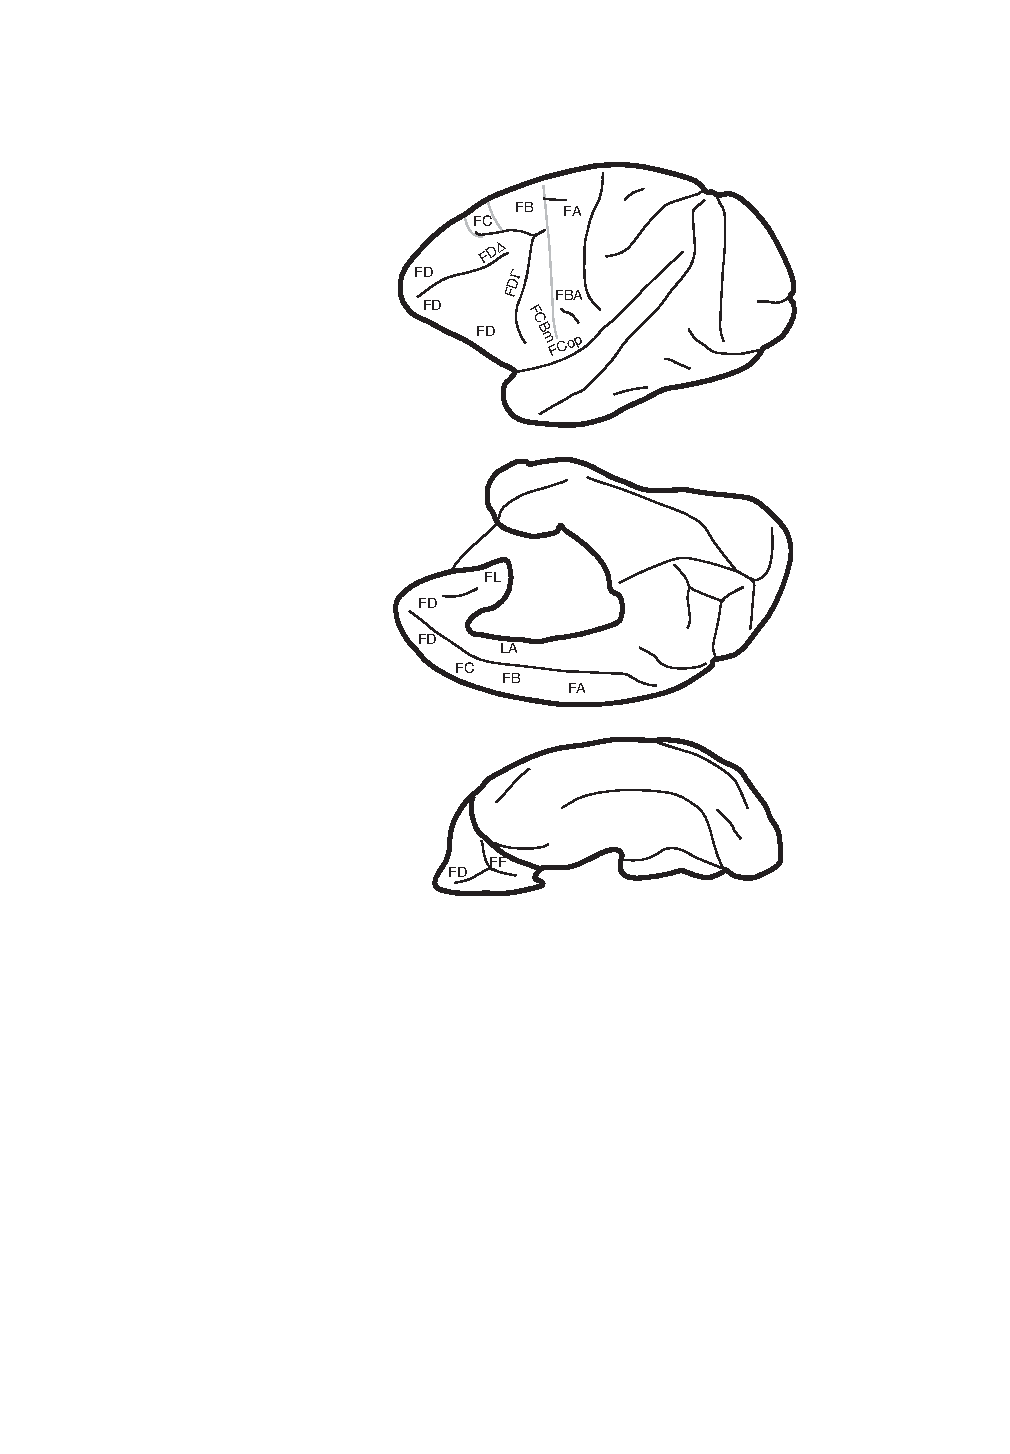
\includegraphics[width=0.5\linewidth]{chap1/1_1}
	\caption{von Bonin和Bailey绘制的猕猴皮层图(1947)。
		吻侧为左侧,顶部为侧位视图(背侧向上),中间为内侧视图(腹侧向上),底部为腹侧视图(侧侧向上)。
		请注意,von Bonin和Bailey将大部分前皮层指定为FD区,尽管他们识别了两个颗粒状区域:FF和FL\cite{von1947neocortex}。\label{fig:1_1}}
\end{figure}
% 必须去除caption后的*,否则交叉引用时会显示?
% 表格和图的\label必须在caption里,否则显示为?

\par
在冯$\cdot$博宁和贝利的命名法中,一个区域名称的第一个字母代表一个脑叶:F代表额叶,P代表顶叶,T代表颞叶,O代表枕叶,L代表边缘。
最后一个字母表示该瓣内的区域;例如,FA表示额叶区域A,与额叶区域B不同。
\par
布罗德曼简单地按照从大脑顶部到底部的顺序对他的区域进行编号,因为他在一系列水平的大脑区域中遇到了这些区域。
所以4区就是从大脑顶部算起的第四个区域。
有时很容易把冯$\cdot$博宁和贝利的命名法和Brodmann命名法的两种命名联系起来:例如,区域FA与区域4相当接近。
但有时,冯$\cdot$博宁和贝利对大脑的看法与布罗德曼截然不同。
\par
如今,通常将这两种命名系统结合在一起,因为它们似乎对某些目的最有用。
“布罗德曼区域”不再需要与布罗德曼自己描述的任何东西相对应,甚至不需要与他想象的任何东西相对应。
\par
除了前额叶皮层的颗粒区和颗粒区外,Brodmann、von Bonin和Bailey等人还发现了介于中间类型的皮层。
颗粒区缺乏的第4层和颗粒区不缺乏的第四层有明显的不同,其他区域具有非颗粒细胞结构。
这种类型的皮质有一个薄的,有时不连续的内部颗粒层。冯$\cdot$博宁和贝利的区域额叶皮层划分有这个属性。
一些区域,如FCBm(图\ref{fig:1_1}),有更多的中间属性,由字母组合指定。
正如我们前面所说的,颗粒状和非颗粒状前额叶皮层之间的区别代表了一种有用的简化,而不是一种严格的二分法。
使用定量分析法证实:当人们沿着前额皮质的内侧或眶面朝上移动时,第4层变得更厚、更明显\cite{mackey2010quantitative}。
\par
在这本书中,我们使用了一个折中的名字组合。
例如,我们使用字母TE和TEO来表示下颞叶皮层,这是由冯$\cdot$博宁和贝利引入的。
我们用6号区域作为运动前皮层,就像布罗德曼用的一样。我们使用了各种变体的大杂烩,例如,在Walker\cite{walker1940cytoarchitectural}之后,极性前额叶皮层使用了10区。



\subsection{前额叶皮层细分}
关于前部皮层的细分还没有达成共识。
正如刚才提到的,冯$\cdot$博宁和贝利只区分出相对较少的额叶区域,但其他解剖学家已经发现了更多。
例如,通过生成猕猴大脑的结构图(图~\ref{fig:1_2}),识别更多的前额叶皮层细分来修改沃克定义的结构图。


\begin{figure}[!htb]
	\centering
	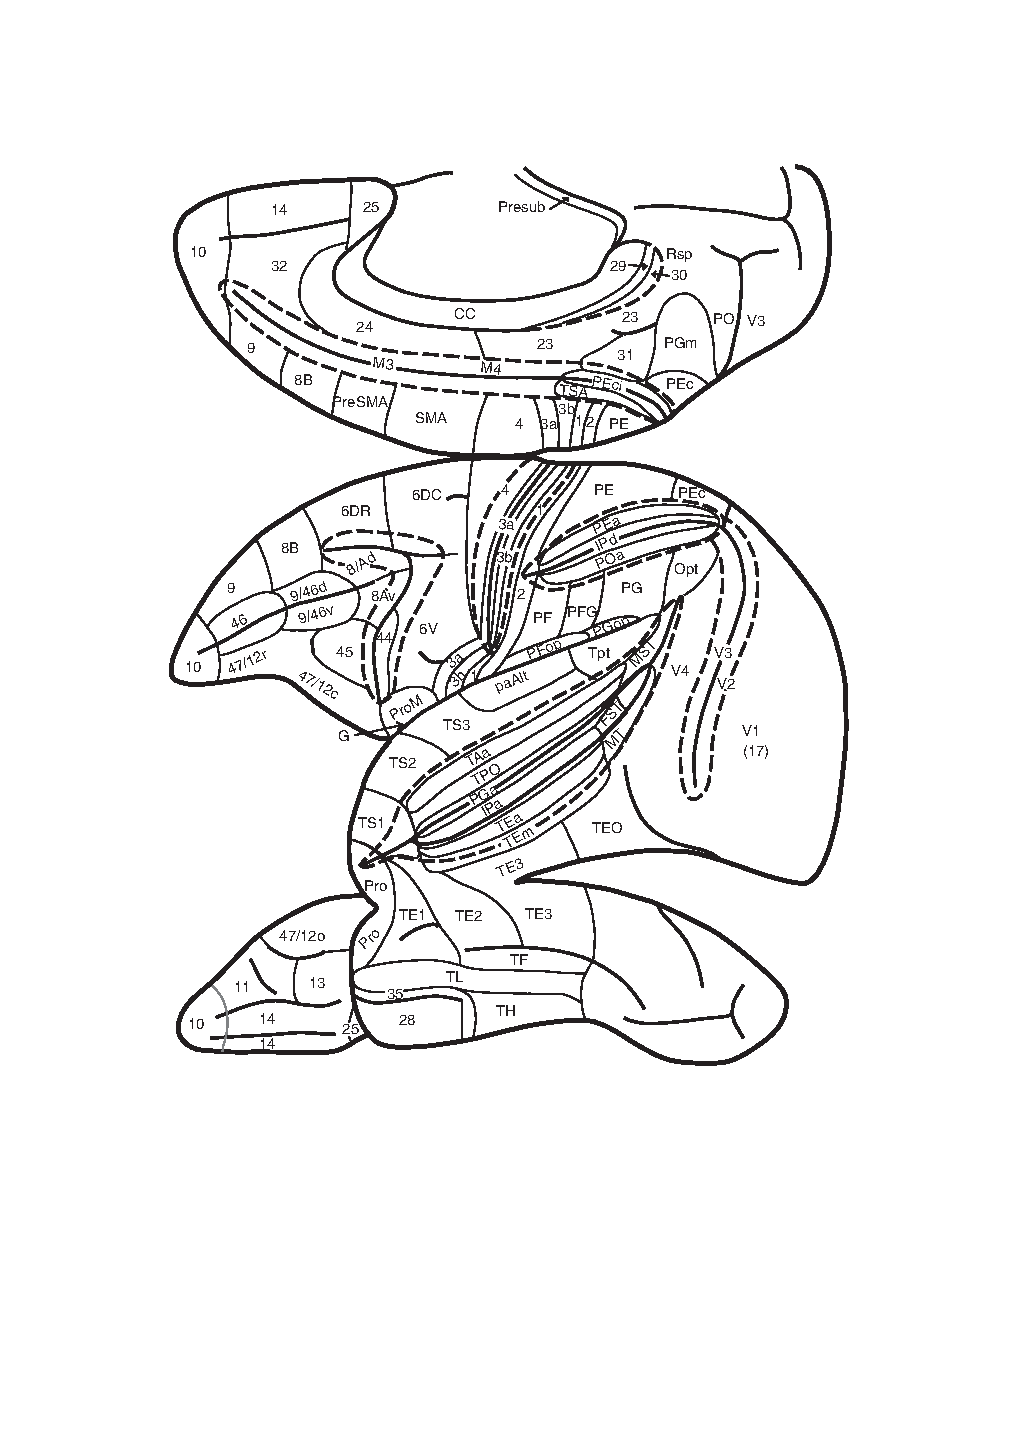
\includegraphics[width=0.65\linewidth]{chap1/1_2}
	\caption{由Petrides和Pandya绘制的猕猴皮层图(2007)。
		吻侧向左,内侧视图在顶部(腹侧向上),外侧视图在中间(背侧向上),底部腹侧视图(外侧向上)。
		缩写:CC,胼胝体;G,味觉皮层;Rsp,脾后皮质;Pro,前皮质,新皮层的变体;PreSMA,预辅助运动区;SMA,辅助运动区。
		区域的细分通常被指定为背(d或d)、吻(r或r)、腹(v或v)、眶(o)、眼(op)、内侧(m)、尾(c)或前(a)\cite{petrides2007efferent}。\label{fig:1_2}}
\end{figure}


\par
通过绘制了人类大脑皮层图(图~\ref{fig:1_3}),与他们的猴子大脑皮层图非常吻合\cite{petrides1995impairments}。
然而,Carmichael和Price(1994)对大脑的看法不同\cite{carmichael1994architectonic}。
他们研究了猴子前脑皮层的眶面和内侧表面,发现了比Petrides和Pandya更多的细分,Öngür等人(2003)对人类大脑也做了同样的研究\cite{ongur2003architectonic}。

\par
神经解剖学家发表了相互矛盾的大脑前额叶皮层图,因为他们在是否以及在哪里检测到边界的问题上存在分歧。
在大脑皮层的其他几个部分,神经生理学通过了地形图来帮助定义一个区域。
在视觉、听觉和体感进行了区域划分,通常会定义一个区域及其边界。
神经生理学对前额叶皮层没有这样的帮助。
同样,不同区域的连接也帮助定义了大脑皮层。
\par
剩下的就是通过加入建筑学知识理解大脑皮层的区域划分,即通过选定的结构特征来识别区域的艺术,称之为皮层建筑学。
当这些区域的特征是依赖于染色的细胞体时,这种做法被称为细胞结构学。
当它们依赖于有髓鞘纤维的模式时,就称为髓结构学。
这两种方法合在一起被统称为皮层建筑学。
退一步说,这是一门不精确的科学。
从本质上讲,皮层建筑学是一种非常高维的模式识别技能,需要多年才能掌握。
因此,几十年来,一种客观、可靠、快速的标记边界的方法一直是皮层建筑学的圣杯。


\begin{figure}[!htb]
	\centering
	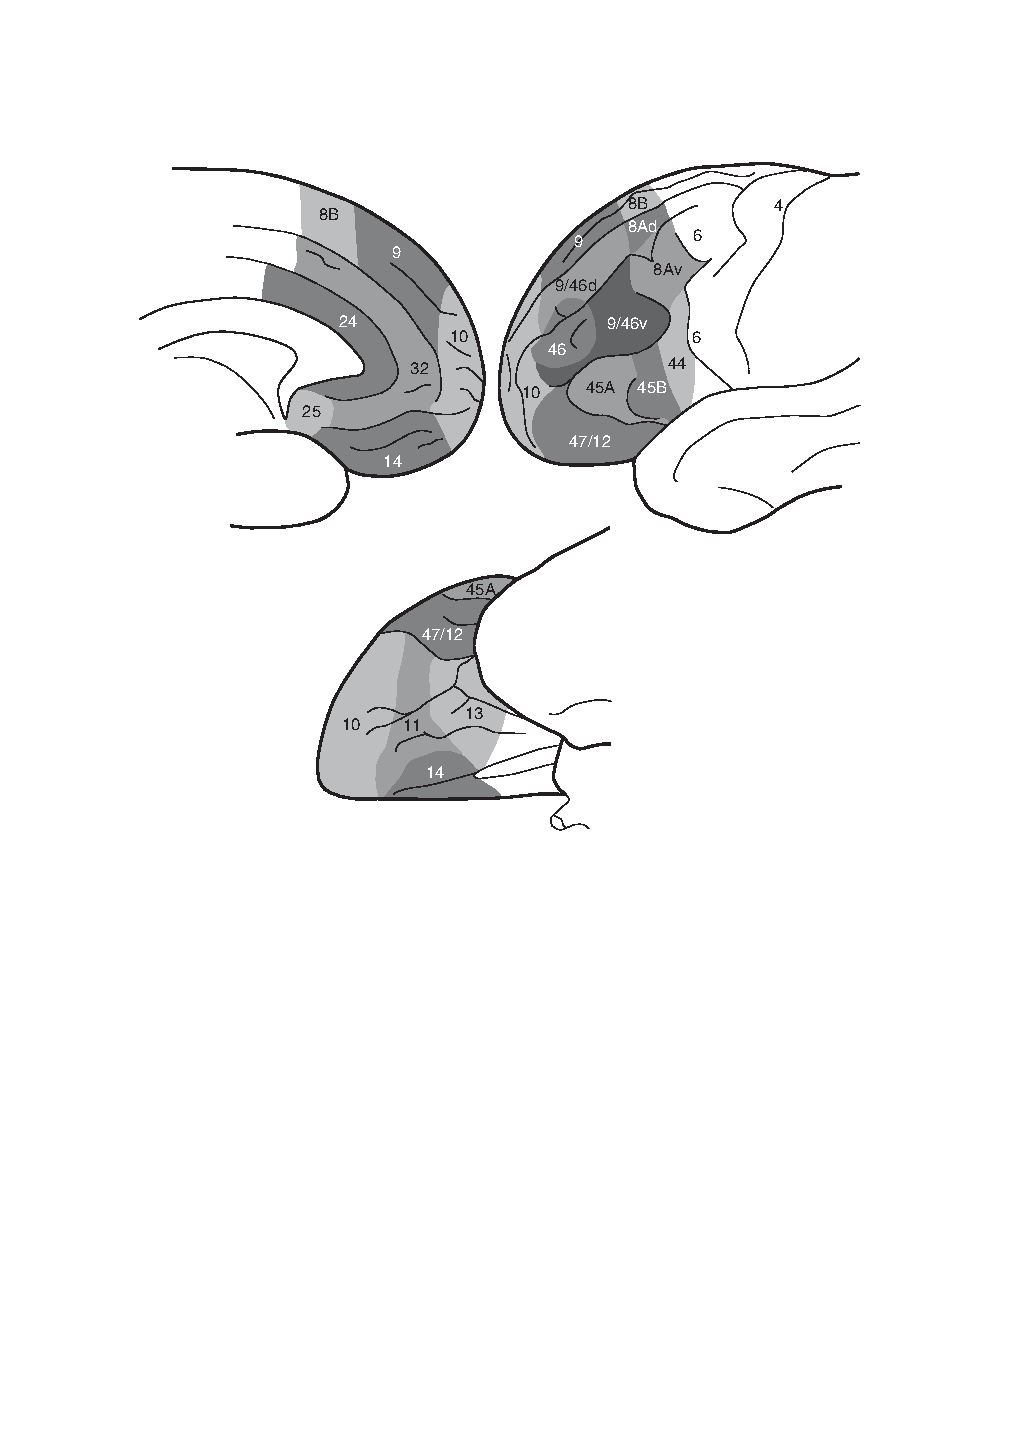
\includegraphics[width=0.5\linewidth]{chap1/1_3}
	\caption{Petrides和Pandya绘制的人类皮层图\cite{petrides1999dorsolateral}。
		在内侧视图(左上),吻侧在右侧;在侧视图(右上),吻侧在左侧;在腹侧视图中(底部),侧面是向上的。
		背外侧前额叶皮层:人类和猕猴大脑的细胞结构分析和皮质连接模式的比较。\label{fig:1_3}}
\end{figure}


\par
Schleicher等人探索了一种他们称之为“观察者独立”的方法\cite{schleicher1999observer}。
他们的意思是,人类观察者不会检测到边界,而是由计算机来检测。
细胞密度从最浅层(第1层)到最深层(第6层)变化。
光密度测量可以反映这种变化,之间的差异反映了不同层中细胞类型和堆积密度的差异。
沿着皮层进行这些测量,加入统计方法可以检测出在不同皮层区域之间划分边界的显著变化。
因此,我们有希望有一天,我们将有一个完整的猕猴皮层地图基于观察者独立的方法,但目前我们还没有找到。

\par
即使可以精确可靠地建立区域边界,它们也可能不对应于功能细分。
例如,在初级运动皮层- Brodmann命名法的4区和von Bonin和Bailey命名法的的FA区-其内侧和外侧的细胞结构不同,内侧的细胞体更大。
但这种特性仅仅是因为内侧运动皮层控制腿部,轴突向脊髓下方延伸,有很大的细胞体。
细胞结构上的差异并不对应于功能上的差异,而是涉及身体不同部位的差异。
如果解剖学家在左脑前部皮层中发现了类似的差异,会将这两个区域标记为单独的区域。
但是,这种区别可能很少或根本没有说明功能。

\par
鉴于在识别前额叶皮层的功能细分方面存在的问题和不一致,我们选择使用一般的描述性术语。
图~\ref{fig:1_4}~显示了猕猴大脑的这些术语;
图~\ref{fig:1_5}~显示了它们与沟和编号区域的关系。


这种方法的优点是不与任何特定的划分图绑定,同时与大多数其他的命名划分图保持一致。


\begin{figure}[!htb]
	\centering
	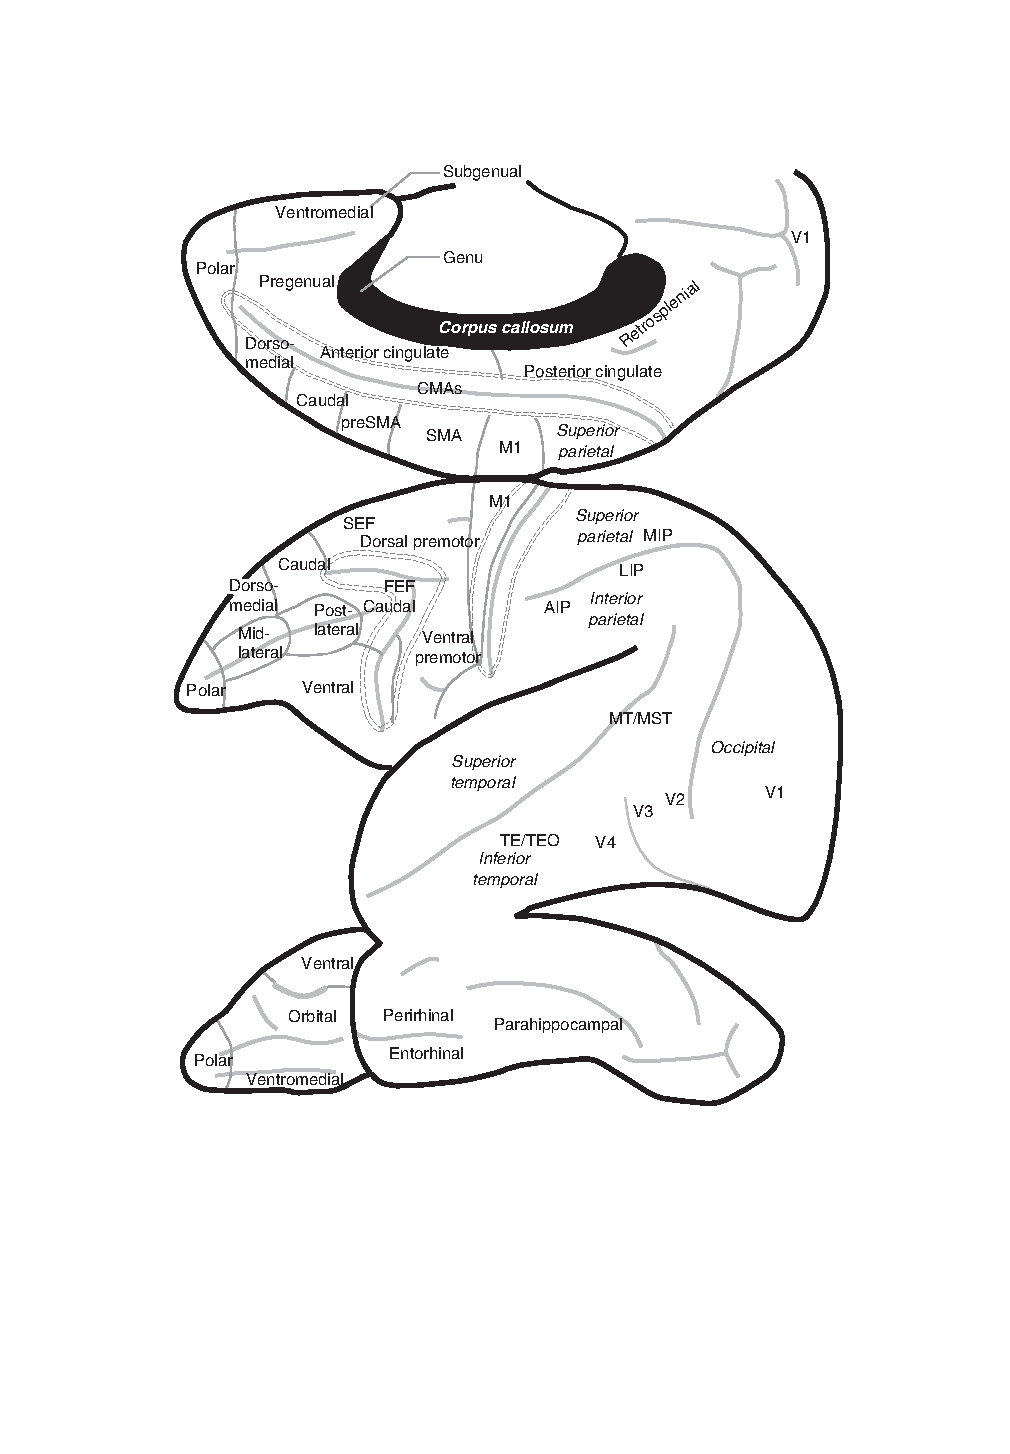
\includegraphics[width=0.6\linewidth]{chap1/1_4}
	\caption{本书中使用的对猕猴大脑的皮层分区的命名分区图。
		格式如图~\ref{fig:1_2}~所示。
		缩略语:参见缩略语列表~\ref{tab:0_1}。\label{fig:1_4}}
\end{figure}




\subsection{约定和缩写}
我们的关于皮层划分的定义主要取决于前额叶皮层的连接解剖学。
因此,当我们回顾成像研究的结果时,我们有时会检查激活的峰值在哪里,以便将它们与我们所知道的猴子的同源区域联系起来。
为了做到这一点,我们使用了\href{http://www.cabiatl.com/mricro/MRIcro/index.html}{MRIcro程序},它采用报告的激活位点坐标,并显示它相对于旋回和沟状地标的位置。
因此,我们对大脑活动定位的描述有时与原作者的不同。
我们希望他们能原谅我们的冒昧。


\subsection{本节小结}
考虑到不同前额叶区域的各种标签,我们请读者参考表~\ref{tab:1_1}~和~\ref{tab:1_2}~进行阅读。
本章中的表格和数字需要注意一下。
在猕猴和人类大脑皮层的某些部分使用相同的名称是很容易的;要确定这些区域就是它们的共同名称所暗含的信息:从共同祖先那里继承的同源物,则完全是另一回事。
第~\ref{chap:chap2}~章主要讨论了这个问题。


\begin{figure}[!htb]
	\centering
	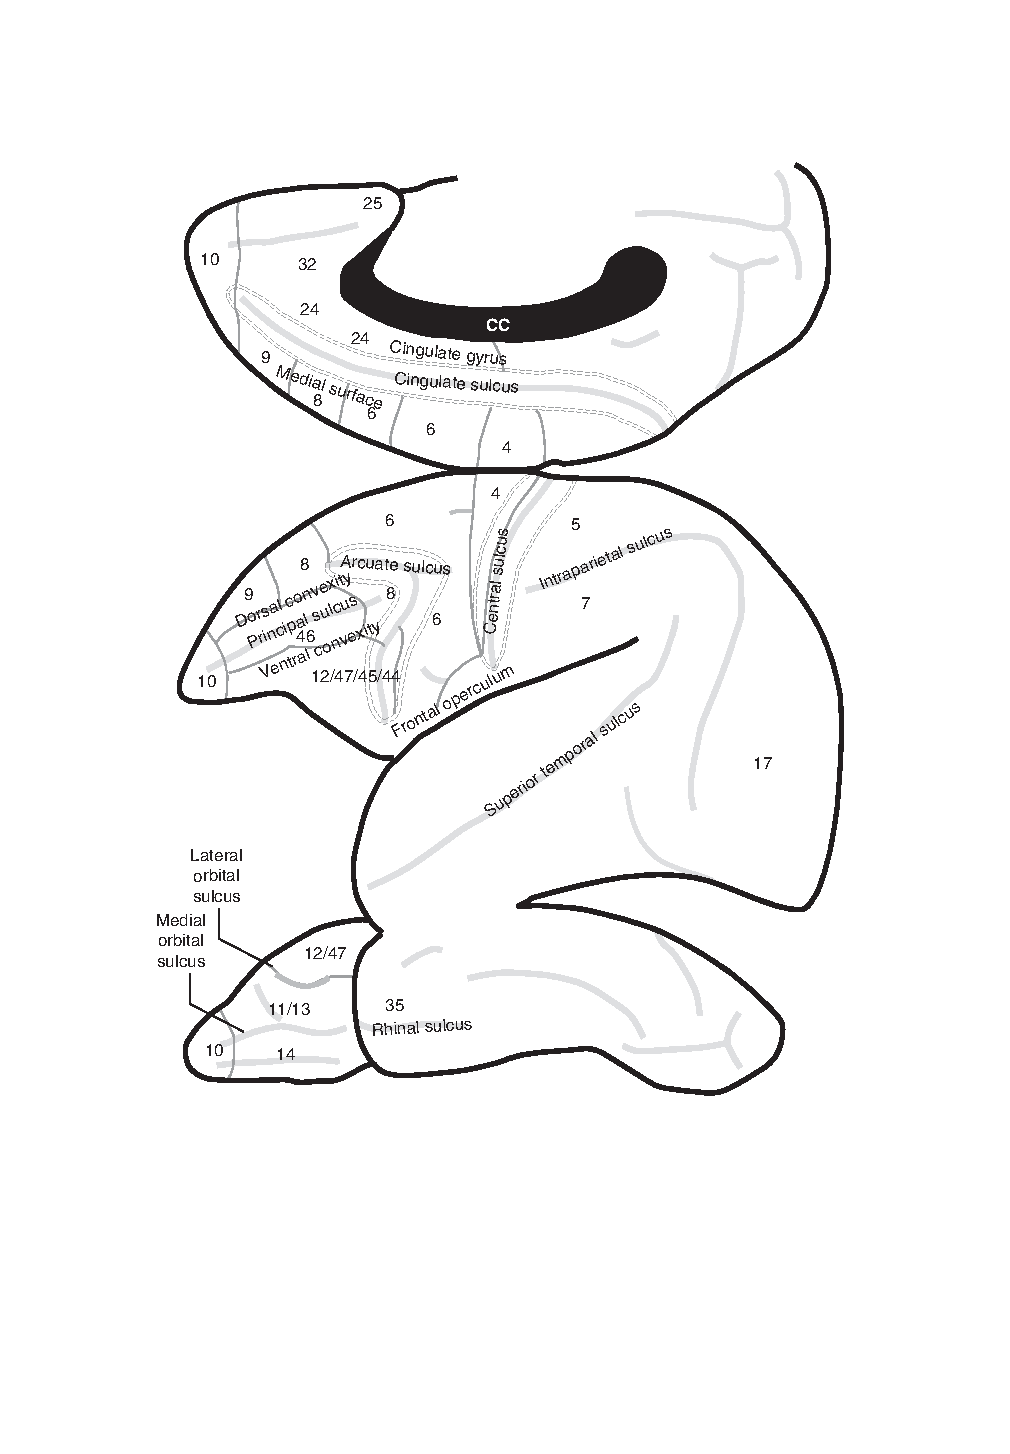
\includegraphics[width=0.5\linewidth]{chap1/1_5}
	\caption{图~\ref{fig:1_4}~中区域命名与皮质区、选定的脑沟和脑回的对应关系图。
		格式如图~\ref{fig:1_2}~所示。
		缩写:cc,胼胝体。\label{fig:1_5}}
\end{figure}



\section{指纹}

现在我们转向一个关键概念,它是我们第二个目标和第三个目标的核心。
一个成功的关于前额叶皮层的理论不仅要解释它的作用,还要解释为什么只有前额叶皮层能做到特定的目标。
为了实现这些目标,我们依靠“指纹”。
用这个比喻来描述一个极坐标图\cite{zilles2001cyto},该极坐标图显示了皮层区域中各种神经递质受体和转运体的密度。
就像在法医科学中一样,神经递质“指纹”具有基于许多特征的识别功能。
将一个区域的整体连接模式称为其连接指纹\cite{2002Dorsal},正如我们在本章节的研究所做的那样。


\subsection{连接指纹图谱}

关于皮质连接的正式研究始于1969年\cite{pandya1969cortico}以及1970年\cite{jones1970anatomical},并一直持续到今天。
当然,随着方法变得更加敏感和可靠,以及其他原因,结果也会发生变化。
\par
例如,在不同的时间,基底神经节的输出被认为只针对辅助运动区(SMA)\cite{schell1984origin};
同时针对初级运动皮层(第4区)和前运动皮层(第6区)\cite{kemp1971connexions};
或瞄准其他区域,包括前辅助运动区(preSMA)、扣带运动区(CMAs)和颗粒状前部皮层\cite{matelli1996thalamic,mcfarland2002thalamic}。
最近的证据表明,基底神经节的输出也延伸到顶叶\cite{clower2005basal}和颞叶\cite{middleton1996temporal}。
毫无疑问,人们所接受的解剖结构总有一天会再次改变,但现在我们只能将按照现有的结果继续研究。
\par
皮层区域的连接指纹具有重要的作用,连接指纹很大程度上限制了相关区域的功能。
例如:如果没有视觉输入,皮层区域就不能执行视觉功能。
利用解剖学数据库中的数据绘制了前额叶皮层不同部分之间的连接图\cite{2002Dorsal}。
该数据库名为\href{http://www.cocomac.org/}{Cocomac},是指猕猴的实际连接。
在最新的版本中,它包含了来自413项研究的39,748个连接条目的数据。
\par
利用这些连接数据研究\cite{2002Dorsal},实验结果表明每个前额叶区域都有一组独特的输入和输出。
对于每个前额叶区域,他们用极坐标绘制出连接的强度。
图~\ref{fig:1_6}~显示了两个相连的指纹,一个位于前部前部皮层的背部(区域9),另一个位于眶前部前部皮层的内侧(区域14)。 
周长表示与特色区域相连的区域,半径表示每个连接的主观强度,范围从1到3。

\par
Passingham等人也使用多维尺度来研究这些联系\cite{2002Dorsal}。
如图~\ref{fig:1_7}A~所示,多维缩放显示没有两个区域具有完全相同的连接模式。
最近也使用Cocomac数据库绘制了各个前额叶区域的远距离皮层-皮层连接图\cite{averbeck2008statistical}。
他们证实,每个前额叶区域都有独特的连接模式。


\par
大脑的任何一个区域都不是单独活动的,所以我们需要把前脑皮层的每个部分作为一个整体来理解。
因此,继续使用分层聚类分析来表明\cite{2002Dorsal},在前额叶皮层内,人们可以识别具有相似连接的区域簇。
使用了一种不同的技术来定义这样的集群,并得出了类似的结论\cite{averbeck2008statistical}。


\par
图~\ref{fig:1_7}B~显示了前额叶皮层内的五个簇\cite{2002Dorsal}。
与Averbeck\cite{averbeck2008statistical}的分析一样,不同簇的功能完全取决于连接。
然而,当人们将这些基于连接的集群与前脑皮层中每个区域的位置信息结合起来时,就会出现一个略有不同的观点。
出于这个原因,我们使用了一个与Price\cite{price2010neurocircuitry}提出的方案非常相似的方案。
他们识别出前额皮层的五个部分:内侧、眶部、尾部、背侧和腹侧。
第~\ref{chap:chap3}-\ref{chap:chap7}~章逐章考虑这五个区域,图~\ref{fig:1_8}~说明了它们。
在很大程度上,这些划分与传统的关于前脑皮层的观点一致。


\par
例如,图~\ref{fig:1_7}~A支持猕猴的极性前部皮层包含在内侧前部皮层中。
每个区域都是一个更大的区域网络的一部分,包括前运动皮层、顶叶皮层、颞叶皮层和海马皮层。


\par
关于广泛的分布式神经网络的发现带来了挑战,这与我们的第二个和第三个目标有关。
在网络中放置前额叶区域是不够的,还需要说明该区域与同一网络中的其他区域在哪些方面不同。
以神经网络为例,它包括中外侧前部皮层(46区)以及后顶叶皮层的几个部分。
这两个神经网络的病变会对行为产生截然不同的影响。


\par
延迟交替任务的经典版本要求猴子学会在一次试验中选择左边的食物井,在下一次试验中选择右边的食物井,以此类推,从而从一次试验到另一次试验交替进行。
中外侧前部皮层(46区)受损的猴子无法重新学习这项任务\cite{butters1969retention},但后顶叶皮层受损则没有影响\cite{ettlinger1966tactile}。
解释必须是,尽管中外侧前部皮层和后顶叶区共享许多连接,尤其是彼此之间,但它们并不是共享所有的连接。
每个区域的连接指纹导致了重要的差异。


\begin{figure}[!htb]
	\centering
	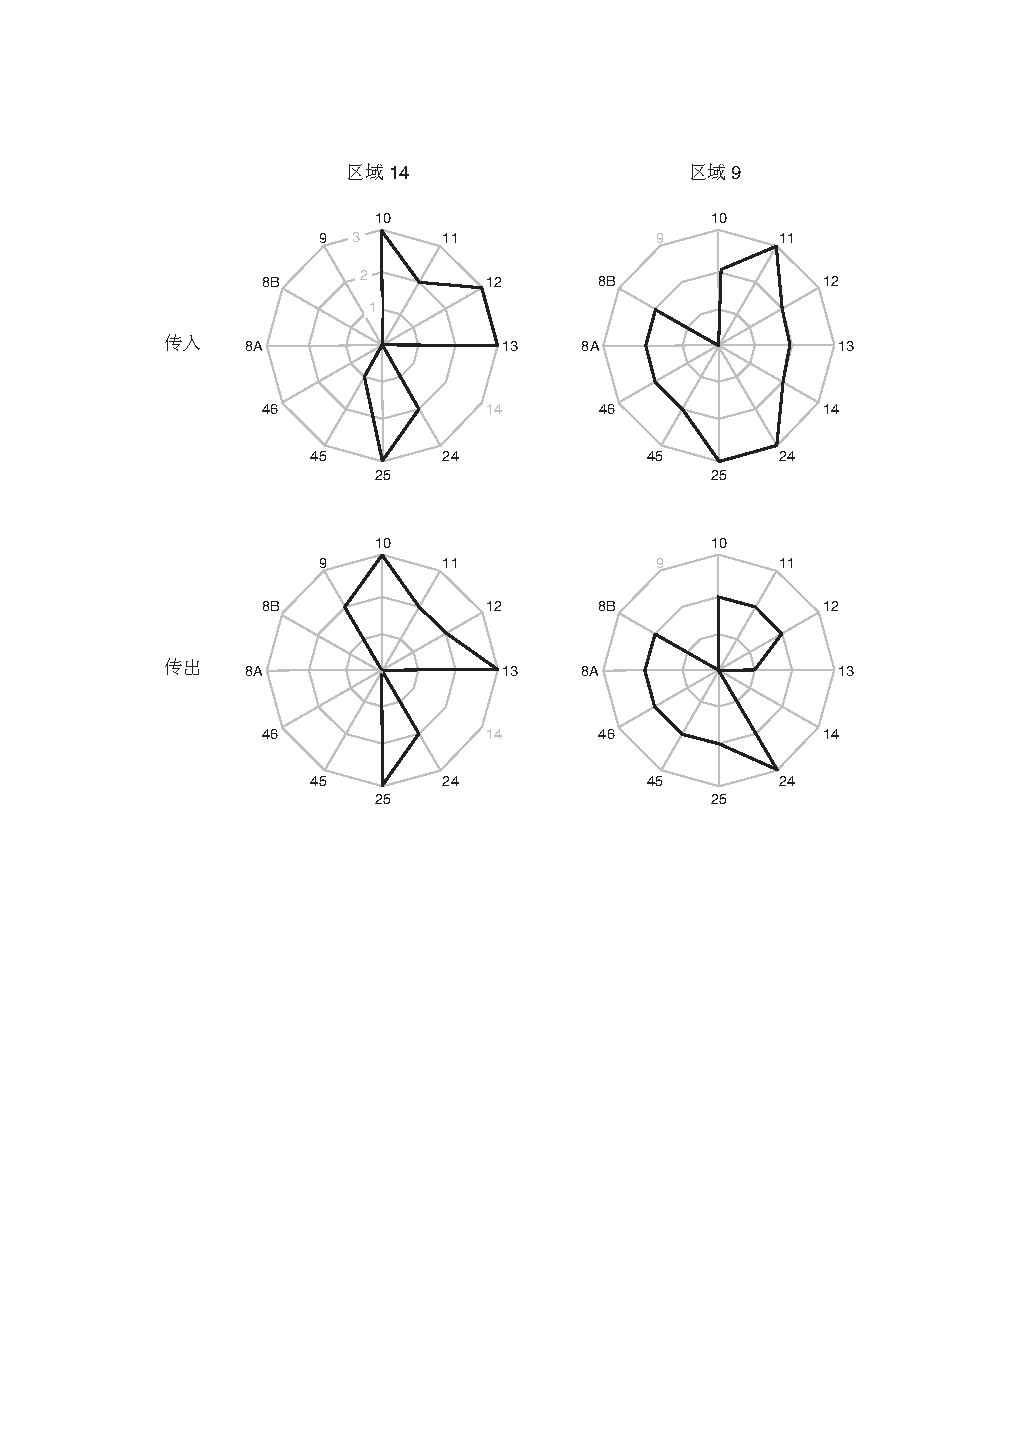
\includegraphics[width=0.65\linewidth]{chap1/1_6}
	\caption{背内侧前部皮层(9区)和部分眶前部皮层(14区)的连接指纹图谱。
		每个极坐标图显示了周边与区域9或14相连的区域,并主观评估了沿半径的投影强度:轻(1)、中等(2)或重(3)。
		例如,左上角的图显示,区域14与区域10有“重”连接。
		区域内的投影不包括在内(圆周上的灰色标签)\cite{2002Dorsal}。 \label{fig:1_6}}
\end{figure}

\begin{figure}[!htb]
	\centering
	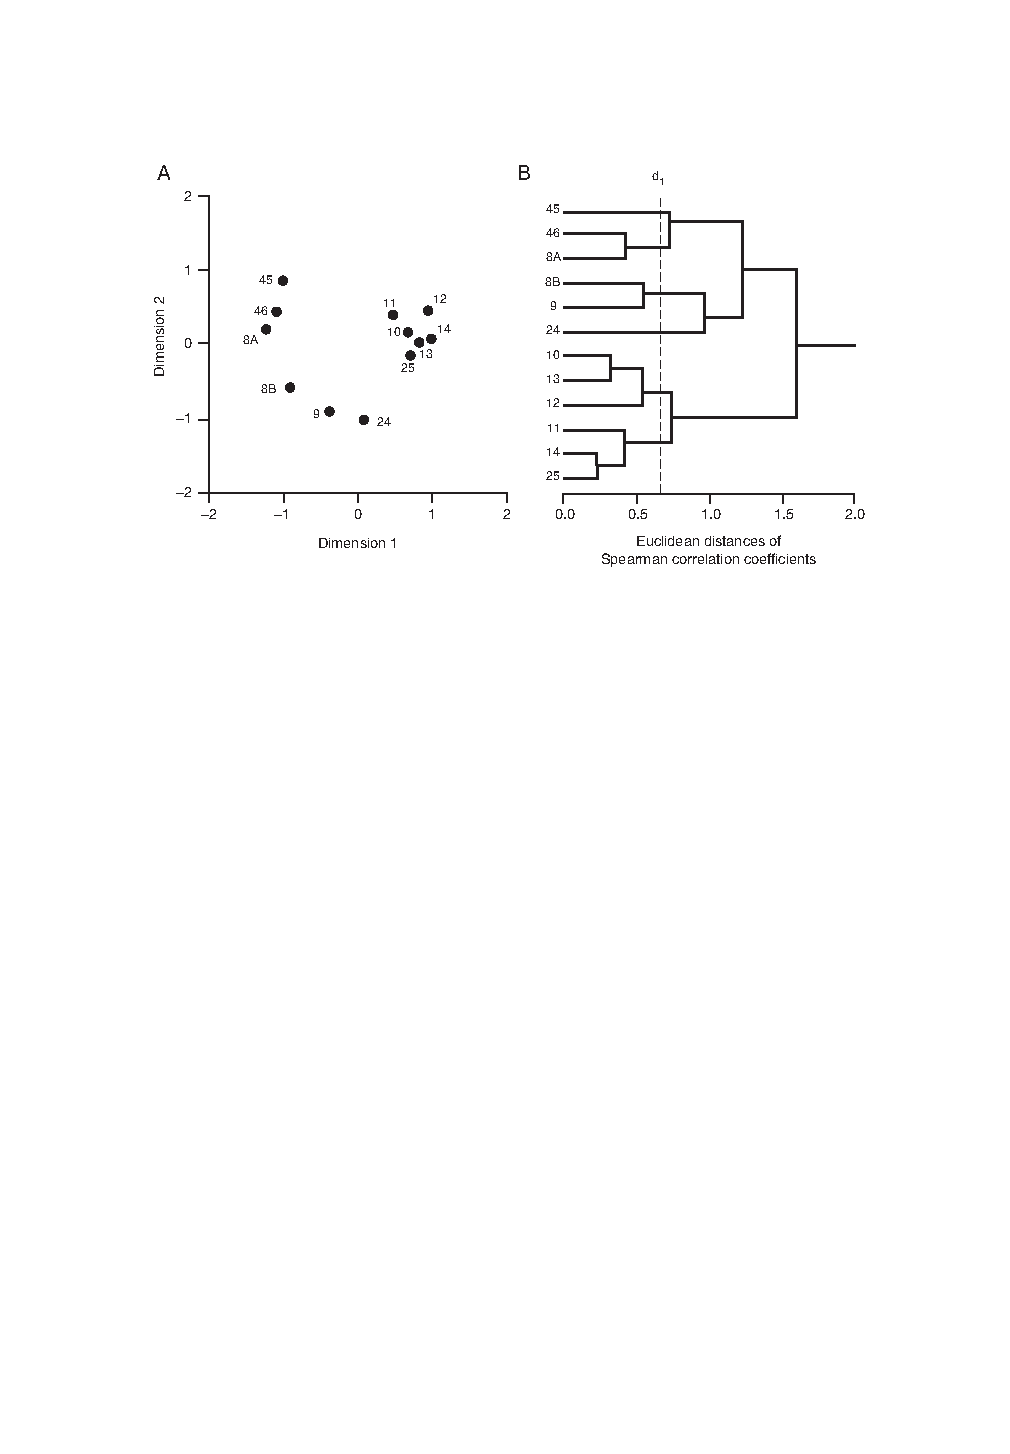
\includegraphics[width=0.8\linewidth]{chap1/1_7}
	\caption{前脑皮层的连接簇图。
		(A)两个连通维度的图,每个点旁边的面积用数字表示。
		(B)沿连接维度的分离分层聚类,记为d1 \cite{2002Dorsal}。\label{fig:1_7}}
\end{figure}


\subsection{生理指纹图谱}

一个区域的连接指纹显示了该区域的约束和功能。
通过类推,引入了功能指纹的概念\cite{2002Dorsal}。
他们用生理数据说明了这些特性,所以我们在这里使用生理指纹这个短语。
对于一组数据,他们绘制了细胞活动的 5 种特性: 
(1)听觉或视觉响应;
(2)本体感觉或皮肤响应;
(3)类似肌肉的活动模式;
(4)活动与运动的时间相关性;
(5)持续的延迟期活动。

\begin{figure}[!htb]
	\centering
	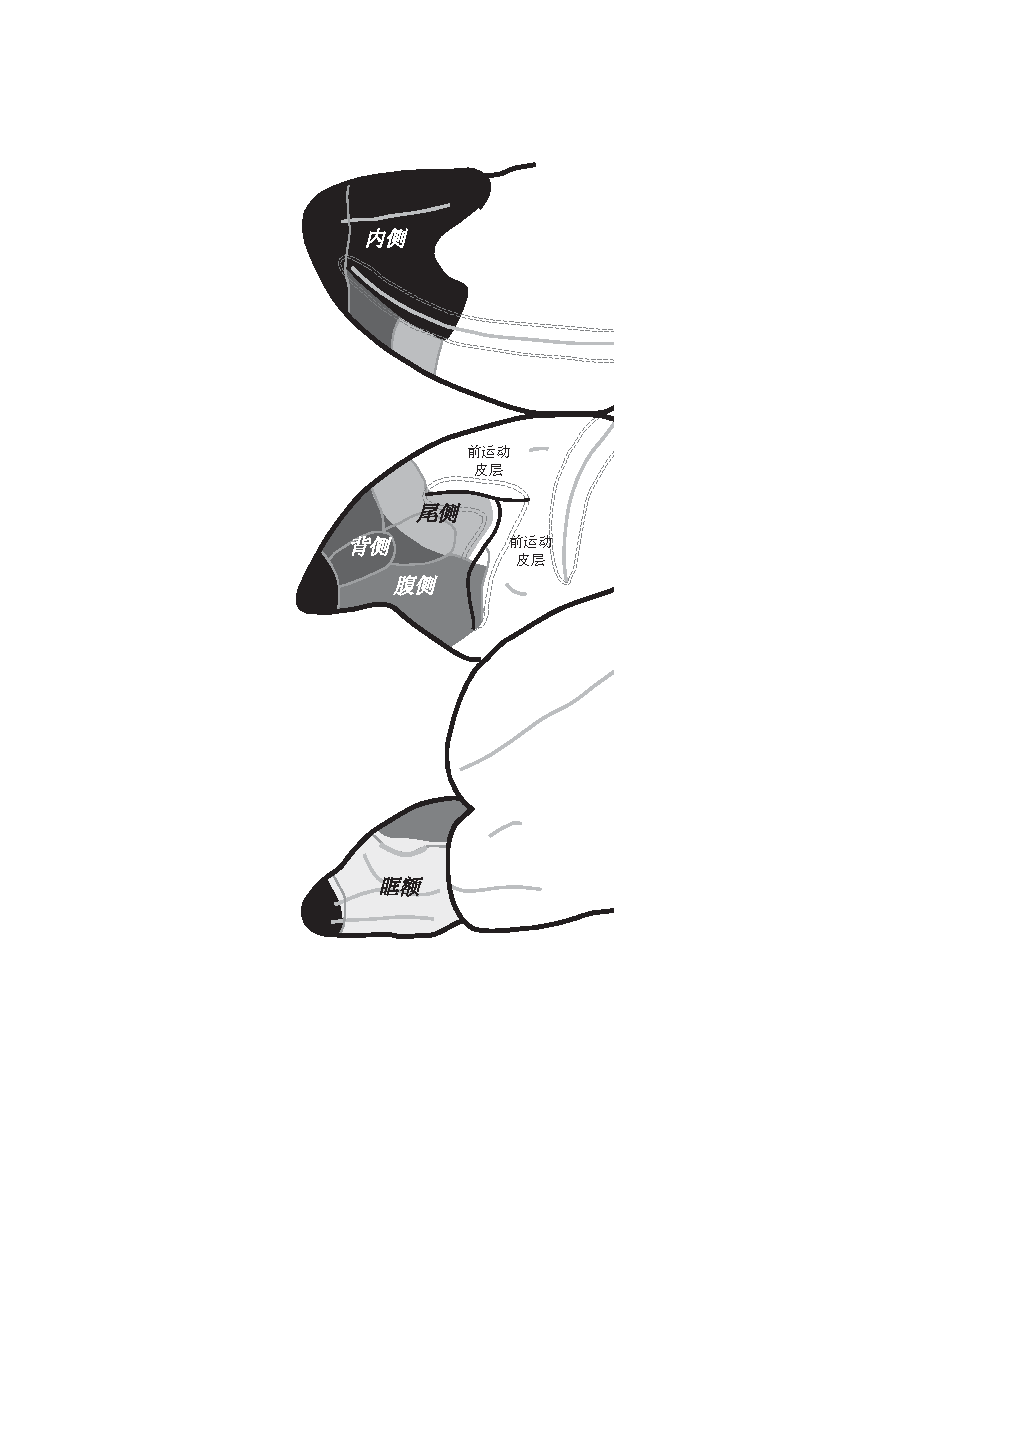
\includegraphics[width=0.35\linewidth]{chap1/1_8}
	\caption{书中用到的前额皮层的 5 个区域图。
		格式如图~\ref{fig:1_2}~所示。
		这 5 个区域中的每一个,内侧前额叶皮层(上)、眶额皮层(下)、尾侧前额叶皮层、背侧前额叶皮层和腹侧前额叶皮层(中)都是后面一章的主题。\label{fig:1_8}}
\end{figure}

\par
如图~\ref{fig:1_9}C~显示,\textit{辅助运动区}和腹侧运动前皮层各细胞类别的相对频率不同。
例如,\textit{辅助运动区}中较高比例的细胞具有体感觉响应。
图中还显示了两个区域连接指纹的不同(图~\ref{fig:1_9}A~和~B)。
\par
对于第二个数据集,Passingham等人(2002)绘制了细胞对根据记忆或基于视觉线索执行的运动序列的偏好\cite{2002Dorsal,mushiake1991neuronal}。
图\ref{fig:1_10}中的直方图显示了\textit{辅助运动区}和运动前皮层的结果,活动分为1到7级。
第一类细胞对视觉任务具有完全的特异性;第七类的细胞对记忆引导的任务有完全的特异性。


\begin{figure}[!htb]
	\centering
	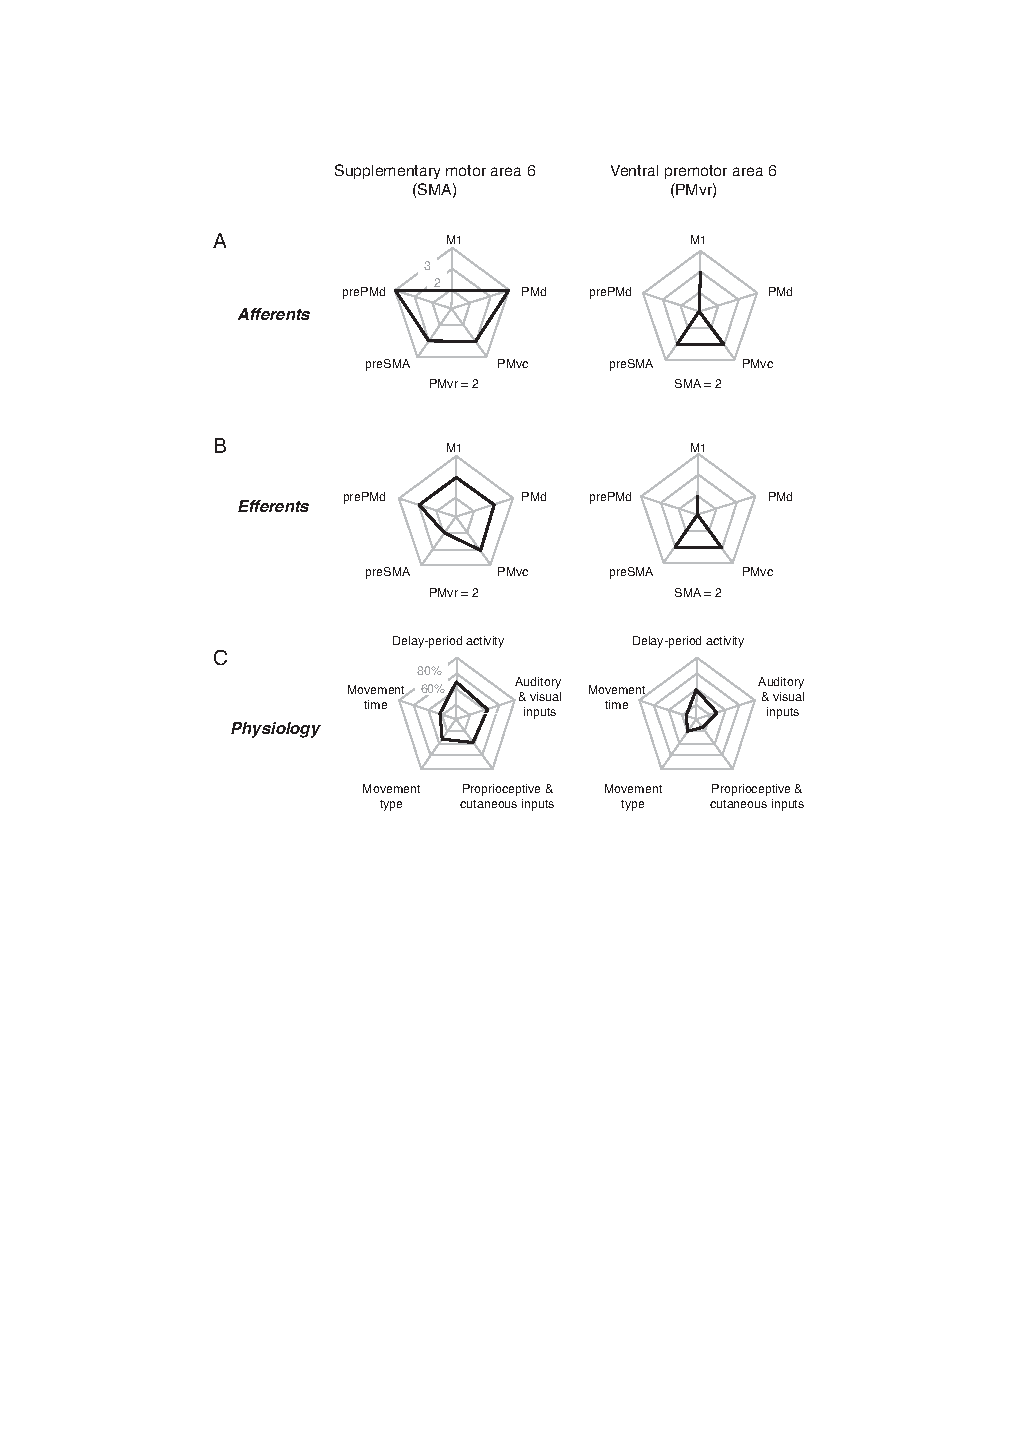
\includegraphics[width=0.8\linewidth]{chap1/1_9}
	\caption{(A,B)辅助运动区(\textit{辅助运动区})和腹侧运动前皮层(PMvr)吻侧的连接指纹图谱。
		缩写:M1,初级运动皮层(第4区);PMd,背侧运动前皮层(6区);PMvc,腹侧运动前皮层尾侧(6区);preSMA,预辅助运动区(6区);prePMd,背侧运动前皮层的吻侧部分(6区)。
		每个极坐标图下面的方程给出了\textit{辅助运动区}和PMvr之间连接的强度。
		(C)同一两个区域的生理指纹图谱\cite{passingham2002anatomical}。	\label{fig:1_9}}
\end{figure}


\par
分类为4表示统计上相等的活动。
\textit{辅助运动区}显示记忆引导任务的活动优势,而外侧运动前皮层显示相反的偏向。
\par
我们还以生理指纹的形式绘制了这些数据。
图~\ref{fig:1_10}~顶部的极坐标图显示的数据与下面的条形图显示的数据相同,单元格类沿圆周绘制,每个类中的比例沿半径绘制。


\begin{figure}[!htb]
	\centering
	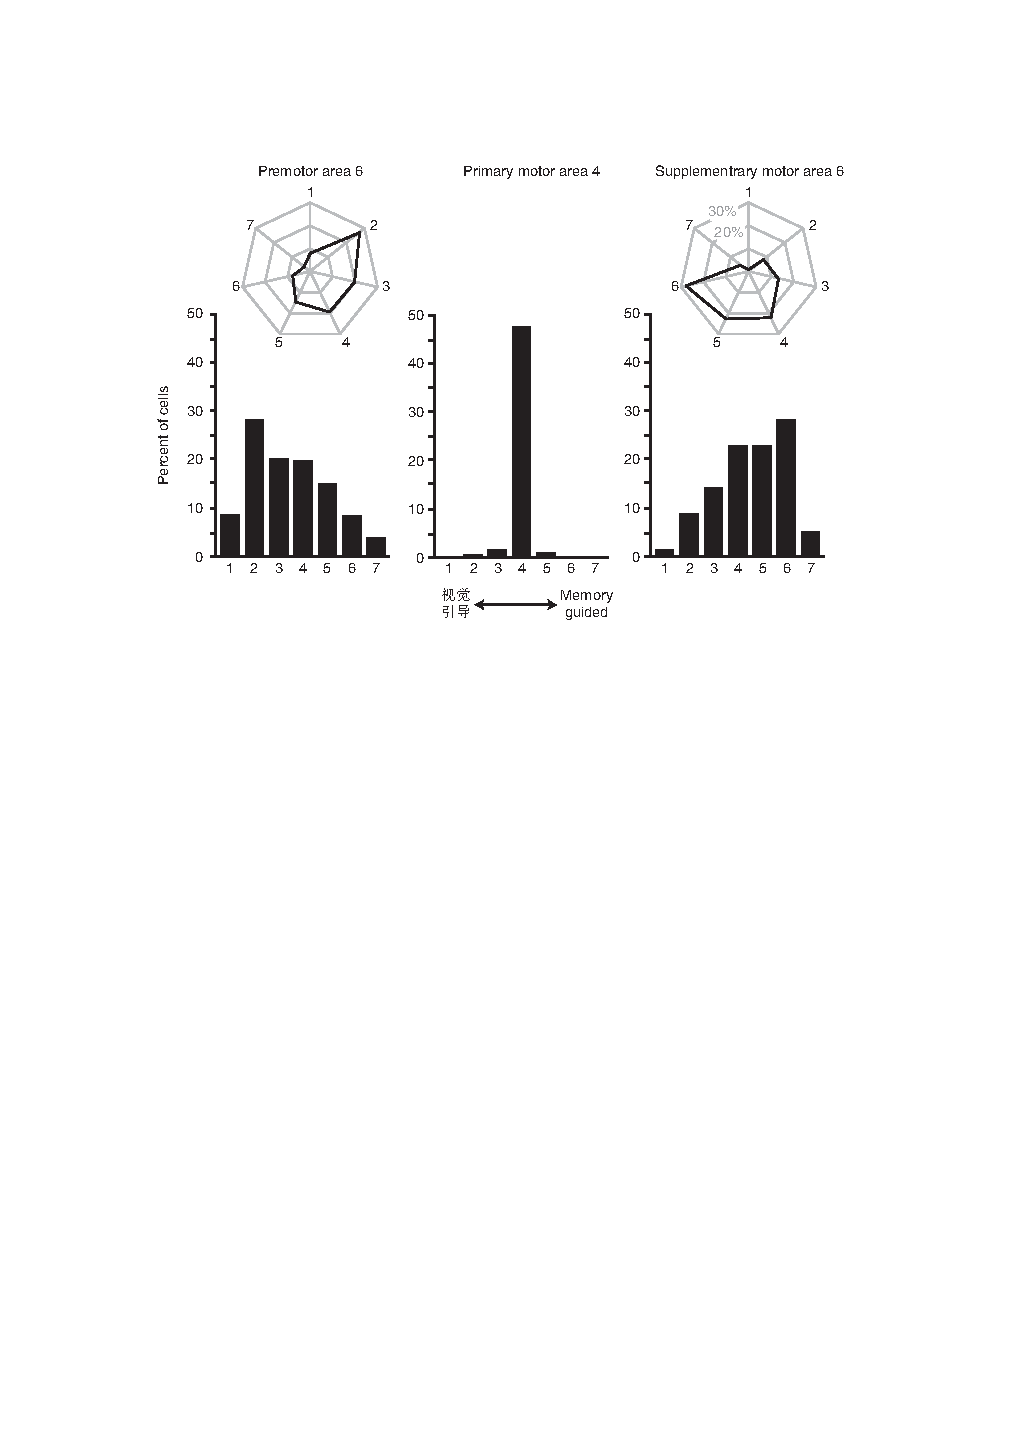
\includegraphics[width=0.8\linewidth]{chap1/1_10}
	\caption{生理指纹显示在运动前皮层(第6区)、初级运动皮层(第4区)和辅助运动区(第6区)对视觉引导和记忆引导的运动序列有选择性对比图。
		第1类细胞对视觉引导序列有完全的特异性。
		第7类细胞对记忆引导序列表现出完全的特异性。
		其他五类细胞表现出中间性质。
		左右柱状图上方的极坐标图显示了与柱状图相同的数据\cite{mushiake1991neuronal}。\label{fig:1_10}}
\end{figure}


\subsection{行为指纹图谱}

到目前为止,我们已经暗示,为了理解前额叶皮层,我们需要比较:通过连接指纹比较区域性质,通过生理指纹比较细胞活动。
从而对行为的理解也会从中加深。
然而,关于前额叶皮层的神经心理学文献往往只强调一些行为任务。
截至2011年,至少有162篇论文发表在对前额叶皮层受损的猴子的延迟响应任务上,其中许多论文只涉及这一任务。


\par
这种专注于一个任务有其优势。
例如,它允许在同一任务上进行行为、生理、成像和药理学实验。
但是,仅仅对一个或几个任务的关注可能会导致对左脑前额叶皮层功能的片面看法。
在第~\ref{chap:chap5}~章和第~\ref{chap:chap6}~章中,我们解释了为什么延迟响应任务和它的近亲延迟交替任务会产生这样的歧义。
从这些研究的结果中得出的结论是:如果功能不是唯一的话,前脑额叶层的功能主要是在工作记忆中。
第~\ref{chap:chap10}~章解释了为什么我们拒绝单一前额叶皮层的理论。
但是,人们不需要知道我们为什么这样做,就能理解仅仅依赖少数任务的问题。
在两个任务的基础上得出前额叶皮层在工作记忆中起作用的结论,就像在参观了两个史密斯奶奶苹果园后得出所有成熟的苹果都是绿的结论一样。
\par
灵长类动物前额额叶皮层的病变会对学习和执行这些任务造成严重而持久的损害,或者有些成熟的苹果是绿色的,我们对此并不怀疑。
灵长类动物的前额叶皮层一定有什么东西使得它对这些任务的执行是必要的。
但需要在任务之间进行比较才能理解它是什么。
因此,除了前面讨论的连接指纹和生理指纹外,我们还需要行为指纹,这涉及到任务之间病变效应的比较。
我们需要了解有前额叶病变的猴子在哪些任务上表现出损伤。


\subsection{本节小结}

一个区域的连接指纹会限制了该区域能做什么。
生理和行为指纹可以让我们深入了解这种功能可能是什么。
许多关于前额叶皮层的理论都是从一个或几个任务的发现中发展出来的。
在第~\ref{chap:chap10}~章中,我们将所谓的通用性测试应用于前额叶皮层的理论,检验它们是否能够解释激发它们的任务之外的数据。
为了确定灵长类动物前额皮层的基本功能,我们需要依靠广泛的研究和发现,如连接、生理和行为指纹的缩影。


\section{病变和激活}

鉴于影像成像技术已经使研究完整的人类大脑成为可能。
有人可能会认为,在试图理解前额叶皮层时,我们不再需要诉诸大脑病变的影响。
毕竟,当应用于人类受试者时,影像成像研究比病变研究有两大优势。
首先,大脑皮层激活部分的峰值位于灰质,而在患者中,大脑皮层病变通常会损害潜在的白质。
其次,峰值可以位于特定区域。相比之下,患者的病变通常包括许多不同的区域。


\par
鉴于这些优点,读者可能会奇怪为什么我们如此强调病变的影响。
我们这样做是因为对某个区域的活动或激活的观察并没有告诉我们,在没有该区域的情况下,受试者是否无法完成任务。
以一项成像研究为例\cite{price1999delineating}。他们的实验对象看到一系列图片,其中一张被指定为目标。
在每次试验中,他们必须从两张图片中选择哪一张与目标有关。
例如,当给他们一把钳子时,他们必须选择扳手而不是锯子。
钳子和扳手在一起是因为它们能抓东西,把它们放在一起需要语义分类。


\par
激活发生在三个地方:左侧颞中皮层、左侧下颞皮层和左侧腹侧前额叶皮层。同时也扫描了一个左腹侧前额皮质完全损伤的病人\cite{price1999delineating}。
病人仍然可以执行任务,即使在任何剩余的前额叶皮层都没有激活。
因此,我们可以得出结论:左腹侧前部皮层对于执行语义分类任务不是必需的,即使它在任务执行过程中显示出激活。
由此我们还可以推断,在腹侧前部皮层没有任何贡献的情况下,中颞叶皮层和下颞叶皮层足以完成任务,我们只有将成像与研究病变的影响结合起来才能得出这个结论。


\par
不幸的是,这种方法很少用于人类大脑研究,因为很难找到只有一个大脑皮层区域病变的患者。
虽然暂时性病变,如重复性经颅磁刺激(rTMS)引起的暂时性病变。
为寻找具有特定病变的患者提供了一种有用的替代方法,但这种方法也有严重的局限性。
人类皮层的大部分深埋在脑沟中,刺激不能选择性地到达它。
此外,刺激效应的精确解剖边界从未为人所知。


\par
由于这个原因,我们的研究在很大程度上依赖于猴子大脑皮层病变影响。
我们可以选择通过使用选择性手术技术,单独切除皮层,而保留底层白质的完整。
人们可以选择性地移除特定区域,特别是在沟槽提供有用指导的地方。
病变的边界可以稍后以合理的准确性评估。作为一种替代方法,人们可以选择性地暂时使某一区域失活。
\par


由于其更高的解剖精度,我们在很大程度上依赖于猴子的实验结果来理解病变效应。
这并不意味着我们完全忽略了对病变患者研究的结果。
这些观察结果可以在几个方面发挥作用。例如,病变对猴子的行为影响可能很难解释,而对人类患者的研究可以帮助解决这些困难。


\par
以两个匹配任务为例。在延迟匹配样本的任务中,猴子首先看到一个物体(样本),在一段时间后,它们必须从两个与样本匹配的物体中选择一个,我们称之为匹配规则。
在延迟的非匹配样本任务中,他们需要选择另一个对象,称之为不匹配规则。


\par
假设前额叶皮层受损的猴子在这些任务中表现有差异。
可能是他们记不住样本,或者无法识别两个物体是相同的还是不同的,也可能是他们不再知道任务规则。
研究前额叶皮层病变患者的一个好处是,我们可以告诉他们规则,然后检查他们是否知道。
如果他们不能正常完成任务,但能告诉实验人员规则,这就证明他们要么忘记了样本,要么在识别两个物体匹配方面存在问题。

\par
这个例子还指出了依赖任务名的危险。匹配和不匹配的任务也被称为“识别记忆任务”。
如果猴子只能以一种方式完成这些任务:记忆和识别物体。
不幸的是,就像在猴子的大脑研究中使用的许多任务一样,这些任务给自己提供了几种替代策略。
猴子可以根据识别、熟悉或最近的情况选择一个物体,这取决于每个实验的细节,有时实验者不知道猴子是如何完成任务的。
具体的比较条件可以区分这些策略,但它们并不总是被使用。
类似地,我们稍后将讨论涉及所谓自定任务的实验。
事实上,是被试还是实验者产生顺序并不重要,所以如果从字面上理解,这个名字可能会产生误导。


\par
然而,只要仔细的解释病变的影像结果,这种方法仍然为一个区域的功能研究提供了一些最重要的证据。
金本位制被称为双重功能解离。
这意味着一个区域的病变会影响一个实验任务的表现,但不会影响另一个实验任务,而其他区域的损伤对两个任务都有相反的影响。
例如,腹侧前部皮层的损伤会破坏猴子执行一种策略任务的能力\cite{baxter2009ventrolateral},而眼眶前部皮层的病变则没有\cite{baxter2007asymmetry,baxter2007orbital}。
相比之下,眼眶前部皮层病变会破坏贬值任务的表现\cite{izquierdo2004bilateral},而腹侧前部皮层病变则不会\cite{baxter2009ventrolateral}。
第 \ref{chap:chap4} 章和第 \ref{chap:chap7} 章详细解释了这些任务及其含义,但即使没有这些细节,我们也可以看到结果建立了某种双重功能分离。


\par
尽管有这些和其他一些例子如 \cite{gaffan2002interaction}指出,这种双重分离在前脑皮层中并不像通常认为的那样常见。
Wilson等人\cite{wilson2010functional}强调,影响整个前额叶皮层的操作通常比主要影响部分的操作产生更大的影响。
这些发现支持了前额叶皮层作为一个整体工作的观点,第 \ref{chap:chap8} 章讨论了这个话题。


\subsection{本节小结}

在一个以成像实验为主导的领域,许多神经科学家似乎认为,在考虑大脑皮层区域的功能时,对损伤效应的理解几乎没有什么帮助。
我们用影像学文献中的一个例子来反驳这一观点:成像激活显示了信息处理的某些方面,但它们并不像病变研究那样显示出在某些任务或功能中所起的必要作用。


\section{病变与细胞活动}

在本章的前一节中,对比了病变和影像成像方法;以及使用切片对比了病变和细胞记录方法。
这两种方法反映了不同的结果。
正因为如此,病变的成像结果并不总是与发生在同一区域的细胞活动相匹配。
我们在前面讨论了一个例子。
在猴子中,中外侧前部皮层(46区)和后顶叶皮层的损伤有不同的影响,尽管这两个区域彼此相连,并且在各种任务中具有相似的细胞活动。
我们之前提到,中外侧前部皮质受损的猴子无法学习延迟交替任务,而后顶叶皮质受损的猴子则能正常完成任务。
然而,中外侧前部皮层\cite{KOJIMA1984229}和后顶叶皮层\cite{chafee1998matching}中的细胞在延迟期(猴子必须记住执行任务所需的信息的时间间隔)中显示出持续的活动。
结果,中外侧前部皮层的细胞活动和损伤效应非常匹配(持续活动和损伤效应),而后顶叶皮层的细胞活动和损伤效应却不匹配(持续活动但无损伤效应)。


\par
另一个例子是运动前额叶区域的内侧和外侧组,它们具有广泛的相互联系\cite{luppino1993corticocortical}。
内侧区域的病变严重破坏了自我产生的运动,被定义为没有视觉提示的运动。
外侧运动前区病变没有这种影响\cite{thaler1995functions};
相反,它们会影响视觉暗示的动作。
考虑到内侧和外侧运动前区都有许多细胞活动,无论运动是视觉提示还是自我引导,这怎么可能呢?
图\ref{fig:1_10}显示,这两个区域的许多细胞都属于第4类,这表明在统计上,这两种引导形式的活动是相同的。
其他细胞表现出偏见,但它们仍然对两项任务都有显著的活动。


\par
要回答这个问题,我们需要认识到,病变研究的结果告诉我们:在没有病变区域的情况下,大脑的其他区域能做什么,不能做什么。
病变不仅消耗了受损区域的计算资源,还消除了其对其他区域的输入以及其他影响。
在完整的大脑中,当动物进行自我引导运动时,外侧运动前皮层的细胞活动显示出增加的活动(图~\ref{fig:1_10}~中的5到7类)\cite{mushiake1991neuronal}。
因此,有人可能会认为,外侧运动前区可以在内侧运动前区缺失的情况下接管自发运动。
但假设这些细胞从内侧运动前区接收输入,这些连接产生了5到7类细胞。
然后,在受损的动物体内,这些细胞将不再具有与正常动物相同的特性。
结果是,在内侧运动前区缺失的情况下,外侧运动前区不能“接管”自主运动。


\par
这种解决思路解释了一个原因,即使某些区域在某些行为中没有发挥必要的作用,它们也会表现出活动。
类似的原理也适用于左脑前额叶皮层。
在一个典型的条件视觉运动任务中,一张图片指示猴子做出一种响应,另一张图片指示猴子做出不同的响应。
细胞在中外侧前额皮层和腹侧前额皮层区域编码这些图像响应映射\cite{asaad1998neural}。
然而,这两个区域的病变的影响是不同的。前部前部皮层腹侧的损伤会对这项任务产生严重的损害\cite{wang2000deficit},而前部前部皮层中外侧的损伤只会产生轻微的影响\cite{petrides2019conditional}。
我们可以用与第一个例子相同的方法来调和这些发现。
腹侧前部皮层的病变切断了颞下皮层向中外侧前部皮层的大部分输入\cite{ungerleider1989projections},因此中外侧前额皮层不能“接管”该功能。


\par
基于病变和细胞记录方法的优缺点,我们需要将细胞活动与脑病变的影像结果进行比较,以便从这两种信息来源中获得最大的好处。
\par
书中不时出现的另一种活动是皮层内微刺激。
这种方法通过与研究单个细胞活动相同的电极引入电流。
因此,它至少在数百个细胞中同步产生活动。
与正常发生的放电进行比较是复杂的,但该方法提供了有用的信息,假设它大致模仿正常活动。


\subsection{本节小结}
大脑皮层的病变的影像结果并不总是像人们所期望的那样与细胞活动相匹配。
在本节中,我们解释了出现这些明显不匹配的一个原因。
病变效应和细胞活动都依赖于一个区域的连接,但方式不同。
细胞活动要么反映通过连接接收信息,要么反映一个区域内的信息处理。
因此,这些结果反映了一种行为的神经相关性,而损伤效应则揭示了一个区域对该行为的必要贡献的行为。


\section{细胞活动和激活}

在后面的章节中,我们将讨论大脑皮层区域激活和细胞活动的发现。
然而,由于两个原因,这种组合需要谨慎:血管伪影和细胞活动与成像激活之间关系的不确定性。

\par
首先,血氧水平依赖信号是一种血管信号,因此它对大动脉的位置很敏感。
BOLD信号也可能受到静脉和静脉流出的位置的污染\cite{turner2002much}。
由于这些原因,BOLD信号的峰值与潜在大脑活动的位置只有非常粗略的空间对应关系\cite{kim2004spatial}。


\par
其次,我们对成像激活和细胞活动之间的关系知之甚少。
对猴子的大脑成像和细胞活动进行直接比较会有所帮助,但要想对前额叶皮层的理解有任何价值,这种比较必须针对稀疏编码的网络进行。
在稀疏编码的网络中,附近的细胞具有不同的性质;
在密集编码的网络中,大多数细胞都做着同样的事情。
由于这种相对同质性,密集编码网络(如感觉或运动区域)的结果可能具有误导性。
我们只有少量关于猴子稀疏编码网络的成像数据,如前皮层或海马体\cite{nakahara2002functional,orban2004comparative}。
所以我们必须运用一般的原则来应付。


\par
成像实验了测量BOLD信号。
BOLD响应可以在没有动作电位的情况下发生\cite{logothetis2002neural},当峰值活动不存在时,BOLD信号可以在不同的实验条件下不同。
例如,Maier等人\cite{maier2008divergence}研究了猴子初级视觉皮层的BOLD激活和单细胞活动。
他们使用了一种称为广义闪光抑制的知觉操纵。
当移动的点突然出现在视觉目标刺激周围时,它们抑制了对目标刺激的感知。
抑制性刺激不影响视觉皮层的单细胞活动,但影响了BOLD信号。
这一发现表明BOLD信号对调节效应很敏感\cite{logothetis2008we},这可能是由抑制性突触输入或低于驱动细胞活动阈值的兴奋性突触输入介导的。


\par
一个研究得特别充分的例子涉及小脑。
虽然突触激活和BOLD信号在小脑皮层密切相关,但其输出神经元浦肯野细胞的活动却不是这样\cite{thomsen2004principal}。
浦肯野细胞的突触输入,而不是浦肯野细胞的活性,驱动BOLD信号\cite{gold2002neuronal}。
浦肯野细胞的两种主要输入:攀爬纤维\cite{offenhauser2005activity}和平行纤维\cite{thomsen2009principal}诱导的局部场电位呈线性增加,而这些电位反映的是突触输入,而不是浦肯野细胞的放电活动。


\par
因此,大多数证据支持这样的结论,即成像研究中测量的信号并不直接反映神经元的活动,而是反映突触的输入。
有时净突触输入(激活)与神经元活动相关,但通常并非如此。
因此,我们在本书中将细胞活动与区域活动区分开来。
我们采用激活来反映突触的影响,而不是单个细胞的放电率\cite{logothetis2002neural}。


\subsection{元分析}

我们前面提到了在解释病变效应时过度依赖一个或几个任务的危险。
同样的谨慎也适用于细胞记录和成像。
在一项经常被引用的研究中\cite{funahashi1989mnemonic},猴子盯着一个中央光点,一个线索出现在八个地方中的一个。
经过一段时间的延迟后,一个“开始”的提示触发了眼球跳动到提示位置。
在延迟期间具有显著活性的细胞中,大多数都编码了线索的位置。
可以理解的是,许多神经科学家认为这一结果与细胞编码记忆位置的观点是一致的。


\par
但是,仅仅根据一项任务得出这样的结论是危险的。细胞活动在某种程度上取决于猴子的训练历史。例如,训练猴子区分猫和狗的图片发现\cite{freedman2006experience},在训练过程中,在不同的方向上呈现的刺激比在不同的方向上呈现的刺激有更强的选择性。
这一发现并不令人惊讶,因为动物(和它们的大脑皮层)从经验中学习。


\par
考虑到这一原则,Funahashi等人\cite{funahashi1989mnemonic}的结果为他们的解释提供的支持比他们想象的要少。
如果只研究简单空间记忆任务中的细胞活动,就会发现似乎许多细胞对记忆的位置进行编码。


\par
但我们只能通过比较其他任务中的细胞活动来验证这种印象。
例如,延迟期的细胞活动可能反映了猴子去的地方以及它们记住的地方。
因此,Lebedev等人\cite{lebedev2004representation}训练猴子既记住一个地点,又去别的地方。
在对某个位置表现出选择性活动的前额叶皮层的细胞中,发现百分之六十一的细胞只编码了参与的位置,而在记忆中的作用被排除在外。
只有百分之十六的细胞单独编码记忆的位置,其余的细胞具有混合属性。
只有任务之间的比较才能表明,从空间记忆的角度对神经元活动的解释在很大程度上是错误的。


\par
在第~\ref{chap:chap8}~章和第~\ref{chap:chap9}~章中,我们通过将许多任务的结果制成表格,认识到这种比较的重要性。
表8.1是对猴子损伤效应的汇总,表8.2是对细胞活性特性的选择。
表9.10对人的成像激活做了类似的处理。
只有考虑到一系列广泛任务的结果,人们才能得出关于左脑前部皮层基本功能的结论。


\par
这种方法类似于影像学文献中常用的方法。
由于结果可以在一个共同的解剖坐标框架中报告,因此可以进行元分析,这涉及到从导致某个区域激活的任务中获得的数据的综合。
元分析是生理指纹的另一个名字。


\subsection{本节小结}

虽然第~\ref{chap:chap3}-\ref{chap:chap7}~章没有使用极坐标图来说明连接、生理或行为指纹,但它们通过更传统的方式传达了相同的原理。
对于神经解剖学数据,他们在猴子的大脑地图上展示了一个特定区域的连接。
他们强调,了解前额叶皮层需要比较不同大脑区域之间的连接(连接指纹),以及比较损伤效应(行为指纹)和各种任务的活动和激活(生理指纹)。
虽然我们在前言中承认了我们挑选的数据,但我们希望读者会同意我们已经尝试挑选了很多数据集。


\par
本节对比了细胞记录和成像结果。像所有方法一样,成像方法也有局限性。
但与细胞活动研究相比,它至少有 3 个主要优势:
\par 1.成像技术允许人们同时观察大脑的大部分区域。
\par 2.血氧水平依赖信号的峰值位置可能反映了特定功能类型信号的峰值密度,而细胞记录将检测到一种类型的活动,无论它发生在哪里。
\par 3.血氧水平依赖信号似乎很好地反映了同步激活。
例如,将脑电图(EEG)和功能成像相结合\cite{parkes2006combining},发现了同步和激活的密切相关性。
BOLD信号与场电位的关系在低频范围内最为密切\cite{kayser2004comparison}。


\par 然而,细胞记录比成像研究有一些优势。
它直接显示了一个区域的信息处理元素所编码的内容。
即使在成像实验中无法检测到不同和混合的神经元群,它也能显示出独特的特性,这对于前额叶皮层这样的稀疏编码神经网络尤其重要。
最后,细胞记录可以区分活动的增加和减少,而成像不能。(成像可以区分活动的增加和减少,但不能区分活动。)对成像文献的讨论很少注意到,例如,激活的增加可能反映了一个区域输出的抑制,这对于稀疏编码的网络尤其如此。


\section{本章小结}

这本书采用对比的方法,以实现对灵长类动物的前额叶皮层的基本功能的定义。它有 5 个明确的目标:
1.描述前额叶皮层赋予的优势;
2.说内部皮层连接如何导致其独特的功能;
3.考虑它如何作为一个整体工作;
4.解释人类进行认知任务期间的大脑激活;
5.解释我们的定义与文献中的其他建议有何不同,以及如何对我们定义的功能进行测试。


\par

为了实现第一个目标,第二章比较了前额叶皮层在不同物种中的发展历程。
为了完成第二个目标,第 \ref{chap:chap3}-\ref{chap:chap7} 章每一章都以对前额叶皮层主要部分的连接的总结开始。
每一章的结尾都简要而具体地介绍了这一部分的功能。
为了实现第三个目标,第~\ref{chap:chap8}~章以第~\ref{chap:chap3}-\ref{chap:chap7}~章的定义为基础,提出了关于前额叶皮层整体基本功能的定义。
为了实现第四个目标,第~\ref{chap:chap9}~章解释了我们如何解释人们执行复杂认知任务时的成像激活。
最后,对于第五个目标,第~\ref{chap:chap10}~章将我们的定义与文献中的其他定义进行比较,提出了一些测试方法,并提出了一些可能与之矛盾的观察结果。









\chapter{灵长类动物前额叶皮层的进化} \label{chap:chap2}









\section{概述}








前额叶皮层的进化经历了不同的阶段。
早期哺乳动物经历了一次进化,产生了所有哺乳动物共有的前额叶皮层颗粒状前额区域。
这些区域的产生能根据预测结果改善行动(第 \ref{chap:chap3} 章)和对象(第 \ref{chap:chap4} 章)之间的觅食选择。
早期灵长类动物经历了另一个进化,形成了第一个颗粒状的前额叶皮层。
原本这些动物的仅在夜间生活于细小的树枝上,它们在那里寻找、选择和获取食物,用一种需要头部和一只手协调运作的方法进食。
他们进化后的前额叶皮层有助于根据当前的生物需求和特定的习惯(第 \ref{chap:chap4} 章)来选择食物,以及在杂乱的环境中保持对食物的注意力(第 \ref{chap:chap5} 章)。
后来,在类人猿灵长类动物的进化过程中,随着这些物种及其大脑体积的增加,出现了额外的颗粒状前额叶皮层。
它们依靠最新进化的灵长类中央凹和改进的色觉在白天觅食。
因此,可以比它们的祖先更好地处理时空事件的顺序(第 \ref{chap:chap6} 章)并对资源的迹象进行检测(第 \ref{chap:chap7} 章)。
因为丰富的资源分散在类人猿的园区范围内,它们面临着严峻的资源波动、捕食和竞争问题。
他们的新前额叶皮层使他们能够通过使用单一事件来选择觅食目标(第 \ref{chap:chap8} 章)来减少风险和非生产性觅食选择的数量。






\section{介绍}

本章探讨了颗粒状前额皮层在早期灵长类动物中首次出现的结果,以及仅灵长类动物拥有这种皮层的事实\cite{preuss2007evolutionary}。

由于其名称,一些神经科学家认为关于颗粒状前额皮层的进化历史仅取决于生物的细胞结构。
考虑到这一主张的重要性,有人可能会争辩说这是一个薄弱的支撑。
幸运的是,许多其他特征支持了“颗粒状前额皮层在灵长类动物中的进化”这一观点。
接下来,我们将列出其中的四个特征:
皮层区域之间的空间布局、颗粒状前额皮层向纹状体的投射模式、感觉输入的分布、以及通过电刺激皮层引起的自主神经反应。






\begin{figure}[!htb]
	\centering
	\includegraphics[width=0.9\linewidth]{image_pfc/Fig_2_1}
	\caption{(A)人类前额皮层的内侧(上)和眶上区(下)\cite{ongur2003architectonic}。 
		(B)猕猴前额皮层的内侧(上)和眶上区(下)\cite{carmichael1994architectonic}。 
		(C)老鼠前额皮层的内侧(上)和侧面(下)
		(Palomero-Gallagher\&Zilles,2004)。
		在所有图中,向左为前端。
		上行:所有图中背面向上。
		下行:(A)和(B)中,侧面向上;
		在(C)中,背面向上。
		不按比例。
		缩写:AC,前扣带皮层;
		AON,前嗅“核”;
		cc,胼胝体;
		Fr2,第二额区;
		la,不含颗粒的岛叶皮层;
		ig,灰脑层;
		IL,下极叶皮层;
		LO,外侧眶上皮层;
		MO,内侧眶上皮层;
		OB,嗅球;
		Pir,锥体(嗅觉)皮层;
		PL,前扣带区;
		tt,盖带;
		VO,腹侧眶上皮层。
		区域细分标记为尾部(c);下(i);侧面(l),内侧(m);眶上(o),后部或极端(p),前端(r),或按任意标记(a,b)。
		(A)改编自Ongur D. Ferry AT,Price JL。《人类眶上和内侧前额皮层的建筑分区》,《比较神经解剖学杂志》460:425-49,2003,经John Wiley和Sons许可使用。 
		(B)改编自Carmichael ST,Price JL.《猕猴颅内和眶上前额皮层的建筑分区》,《比较神经解剖学杂志》346:366-402,1994,经John Wiley和Sons许可使用。 
		(C)改编自Palomero-Gallagher N,Zilles K.《老鼠神经系统》中的异皮层.ed.G Paxinos,pp.729-57.圣迭戈,加利福尼亚州:爱尔斯维尔学术出版社。\label{fig:fig_2_1}}
\end{figure}

图\ref{fig:fig_2_1}展示了我们对人类、猕猴和老鼠这三个物种颗粒状前额皮层的同源性的看法,这主要归功于Preuss\cite{Preuss1991a}的开创性工作。
同源性指的是由于共同祖先的遗传而在相关物种中出现的类似区域。
该图以浅灰色显示了仅在灵长类动物中进化出来的颗粒状前额皮层。
这些颗粒状区域同样出现在人类和猕猴的大脑中,但不出现在老鼠的大脑中。
老鼠只有无颗粒状前额皮层区域,该图为三个物种均以深灰色表示。
我们选择这三个物种,是因为我们对前额皮层的大部分知识都基于对它们的大脑的研究。


非颗粒性前额叶皮层区域包括下边缘皮层、前边缘皮层、无颗粒的岛叶皮层、无颗粒的眶额皮层和前扣带皮层。
在不同物种中,这些区域往往有不同的名称。
例如,啮齿动物的下肢内侧皮层与灵长类动物的25区大致相对应,von Bonin和Bailey将其称为FL区(图\ref{fig:1_1})。


众所周知,许多神经科学家认为老鼠拥有与灵长类动物相同的前额叶皮层。
并且他们坚持认为,老鼠具有模拟灵长类动物前额叶皮层的微型复制品,或者可以将其所有属性混合在他们的小型无颗粒区域中\cite{kolb2007all,seamans2008comparing,schoenbaum2009new}。
虽然我们对此持有不同的观点,但有一个命题应该得到普遍接受:在进化历史的某个时刻,我们的某些祖先缺乏颗粒性前额叶皮层。
然而,现在我们不再缺失它。
鉴于这个历史事实,询问颗粒性前额叶皮层带来了什么优势似乎是合理的。


尽管不是每个人都同意图 \ref{fig:fig_2_1} 所描绘的同源性,但没有人严肃地质疑现代啮齿动物的大脑缺乏颗粒状前额叶皮层这一事实。
对于其他哺乳动物,有一点存在争议:
有人认为狗\cite{rajkowska1988intrinsic}和猫\cite{je1948orbitofrontal}具有颗粒状前额叶皮层区域。
但当我们亲自检查组织学材料中,狗和猫所谓的颗粒状区域时,它们看起来很像猕猴和啮齿动物的无颗粒区域。


\begin{figure}[!htb]
	\centering
	\includegraphics[width=0.8\linewidth]{image_pfc/Fig_2_2}
	\caption{显示了大脑额叶区域从尾向头发展的过程中,第4细胞层的归一化密度在猕猴(黑线)和人类(灰线)中的变化。
		误差条:SEM。
		该图由 Mackey S、Petrides M. 在《欧洲神经科学杂志》2010年32期(1940-1950页)中发表,经John Wiley 和 Sons出版社许可后再版。
		该图表明人类和猕猴大脑的腹内侧和侧壁眶前额皮质中具有可比较的成系统的区域。\label{fig:fig_2_2}}
\end{figure}


正如第 \ref{chap:chap1} 章所述,这种争议可能是由于观察者缺乏成体系的知识方法所致。
当在猕猴和人脑中观察到这个问题时\cite{mackey2010quantitative},发现一些传统上被归类为无颗粒额叶区域的区域实际上在第4层细胞体密度上,与最尾端的区域相比有略微的增加。
也就是说,这些区域具有较弱的非颗粒质细胞结构,而不是完全的无颗粒结构。
在食肉动物和其他非灵长类哺乳动物中发现颗粒状前额叶皮层的报告,反映了这种属性。
神经解剖学家们都认为,细胞从额叶轨道和内侧表面向头部移动时,第4层的厚度会持续增加。
因此,无颗粒皮质是否在第4层完全消失并不重要。
我们可以将第4层密度低于给定阈值的区域视为足够无颗粒这一标准,用于我们之后的研究中(如图 \ref{fig:fig_2_2} 所示)。


尽管老鼠缺乏细颗粒前额皮层,但一些神经科学家仍认为,老鼠前额皮质的中部与灵长类动物的中侧颗粒前额皮层(区域46)同源\cite{kolb2007all},尽管后者的是一个颗粒区域(也称为背外侧或周主前额皮层)。
同样,还有一些人认为,老鼠前额皮质的侧部与灵长类动物的整个眶前颞皮质同源,包括其颗粒部分\cite{kolb2007all,schoenbaum2009new}。
该论点基于解剖学、生理学和神经化学的相似性以及基于声称在老鼠和猕猴中的损伤效应的相似性。


然而,人们不能仅仅依据常被引用的相似性就推断其同源性。正如 Preuss\cite{preuss1995rats}所解释的那样,人们需要对特征进行诊断,即区分一组皮层区域和其他区域的特征。
就像老鼠的非颗粒状前额皮质与猕猴的颗粒状前额皮质区域具有许多相似之处,例如编码估值的细胞。
但是,这三个区域——老鼠的非颗粒状前额皮质以及猕猴的非颗粒状和颗粒状前额皮质——都具有与上述细胞同样的特性,其他皮层区域也是如此。
因此,它们无法帮助我们理解前额皮层皮质的进化或建立其区域之间的同源性。
例如,老鼠的非颗粒状区域的特性与灵长类动物的颗粒状前额皮质相似,但它们也与灵长类动物的非颗粒状前额皮质相似,那么这些特性就与动物的同源性无关。


有人声称,颗粒质前额皮层与丘脑中背核(MD)的联系是其诊断性特征\cite{je1948orbitofrontal,akert1964comparative,uylings2003rats}。
但是,MD核向实际上覆盖了额叶的几乎所有区域,包括颗粒质和非颗粒质区域。
因此,与MD核的连接不能作为诊断性特征,故它们对于同源性的问题几乎没有影响或很少有影响。


曾经有一段时间,人们认为多巴胺能输入是颗粒状前额皮质的特征\cite{divac1978converging,porrino1982brainstem}。
但是这些输入也终止于前额叶皮层的非颗粒状部分和运动前区,以及额叶以外大部分皮质。
事实上,在灵长类动物中,多巴胺输入到运动前皮质和后枕叶皮质的强度比大多数颗粒状前额皮质都要强\cite{gaspar1992topography,williams1998widespread}。
因此,多巴胺输入不能帮助我们跨物种识别前额叶皮层。


最终,损伤结果得到了进一步的研究,例如对于延迟反应任务的研究结果。
老鼠的前额内皮层损伤会导致该任务的障碍\cite{kolb1974double},类似地,猕猴颗粒质前额皮层的损伤也会导致该任务的障碍\cite{goldman1971analysis}。
但是,前扣带回皮层的损伤也会导致猕猴在该任务上出现障碍\cite{meunier1997effects}。
因此,该特征并非是诊断性的。
我们将在第 \ref{chap:chap10} 章中更详细地讨论这个问题,老鼠和猕猴的障碍虽然表面上相似,但在重要的方面存在差异。


值得注意的是,我们并不是说灵长类动物拥有前额皮层而其他哺乳动物没有。
我们认为非灵长类哺乳动物也有一些可以合理称之为前额皮层的区域。
第 \ref{chap:chap3} 章和第 \ref{chap:chap4} 章将这些非颗粒质区域纳入了内侧和眶前颞皮层。
但我们不赞同非灵长类哺乳动物具有类似于灵长类前额皮层的微型复制品或混合体的观点。
非灵长类哺乳动物缺乏灵长类动物的颗粒质前额皮层以及执行其基本功能的任何区域。
因为忽略了这些概念,文献中存在很多将非同源区域的结果混合在一起的实例,例如,引用灵长类动物的中侧前额皮层(46区)的研究结果来支持与啮齿动物的前额内皮层相关的某些结论。但其实这不是最好的方式。


我们对同源性的结论不应该引起太多争议。
以视觉皮层为例,所有灵长类动物都共享10-20个视觉区域,其中有些物种甚至拥有更多的视觉区域\cite{kaas2020evolution}。
举个例子,一个被称为MT或V5的区域在视网膜中央凹有精细的专门分化功能,用于分析视觉运动。
但老鼠的视觉区域少得多\cite{rosa1999evolution,lyon200734},不可能复制灵长类动物10-20个视觉区域的所有功能,并且它们缺乏中央凹。
另外,在缺乏中央凹的物种中进行视网膜中央凹的微观分析是不太可能的。


再以另一个例子为例,考虑到蝙蝠听觉皮层的回声定位功能。
这些动物使用类似声纳的系统来检测它们与猎物的距离和猎物本身的速度。
蝙蝠的听觉皮层有许多专门区域来处理与回声定位相关的声学信号,包括分析调频声音、多普勒频移等\cite{suga1997cortical,fitzpatrick1998distribution}。
但如果老鼠的听觉皮层中的一些细胞也对类似的声音作出反应,这并不意味着它们执行与蝙蝠听觉细胞相同的功能。
事实上,想象它们这样做是很奇怪的,因为老鼠不会用回声定位来追踪它们的食物。
同样,认为老鼠的少数听觉区域具有与回声定位蝙蝠的大量专门区域相同的所有功能和属性是缺乏可信度的。


很少有神经科学家质疑这样一个想法:与老鼠共同祖先相比,声呐定位蝙蝠拥有新的听觉区域,而灵长类动物拥有新的视觉区域,以适应其在视觉敏锐度和色彩视觉方面的需求。
同时,这些新区域支持新的功能,如对凹视动作或回声定位的分析,这一观点已经被广泛接受。
因此,令人惊讶的是,同样的神经科学家们往往对这样一个想法犹豫不决:灵长类动物拥有新的前额区域,并且这些区域具有新的功能。


问题的一部分来自于使用“新”的词来描述区域或功能。
有人提出,新的区域通过复制和随后的分化出现\cite{krubitzer2000arealization}。
如果是这样的话,那么合理的假设是,某些新区域的分化程度比其他区域低;
当它们在许多哺乳动物中出现时,我们可以将更保守的区域识别为同源的。
然而,在这样做时,我们需要认识到大多数进化所产生的变化都涉及到同源结构的修改,因此在物种之间具有绝对等价是不现实的。


相较于这些相对保守的区域,其他的复制产物则更加具有差异化,因此应该被称为新的区域。
随着差异化的产生,它们开始执行新的功能,从而提供了优于其祖先状态的优势。
然而,当这些新区域进化时,它们会与附近的区域共享属性,并且通常会与它们有轴突连接。
因此,虽然前额叶皮层的颗粒层和无颗粒层部分具有许多共同特征。
但是我们不应该基于此得出它们是同源或类似的结论。
颗粒状的前额叶皮层专门在灵长类动物中进化而来,并发展为支持灵长类动物具有特别能力的区域。


\section{原猴亚目前额叶皮层}
灵长类动物前额叶皮层进化的最有力证据来自对原猴亚目的研究。
鉴于这一证据的重要性,我们将详细地回顾它。
然而,读者可以从本节末尾的摘要中了解该论点的要点。

\begin{table}[htbp]
	\newcommand{\tabincell}[2]{\begin{tabular}{@{}#1@{}}#2\end{tabular}} %换行指令
	\centering
	\caption{本章中使用的生物学术语}
	\renewcommand\arraystretch{1.5}	%设置表格内行间距
	\begin{tabular}{ll}
		\toprule
		术语 & 含义 \\
		\midrule
		进化 & 与祖先状态不同,具有差异化的  \\
		埃及古猿 & 一种已灭绝的类人猿,接近早期的狭鼻类动物  \\
		类人猿 & 猕猴、猿类和人类  \\
		食果猴 & 一个已经灭绝的古老哺乳动物类群  \\
		智利猴 & 一个灭绝的类人猿,接近于最早的阔鼻猴  \\
		狭鼻猿& 旧大陆灵长类动物(旧大陆猴、类人猿和人类),从阔鼻猿中分化出来  \\
		类人猿亚目& 眼镜猴与类人猿;从原猴类中分化出来  \\
		同源性& 从共同祖先继承而来的相似性,与由平行或趋同进化引起的相似性形成对比  \\
		旧大陆猴& \tabincell{c}{一组狭鼻猴类灵长目动物,包括猕猴、狒狒、长尾黑颚猴(绿猴)、\\白眉猴、长尾猴、山魈猴和红尾猴}  \\
		%内容换行
		副猿& 已灭绝的类人猿,接近于第一个类人猿,也被称为Simonsius  \\
		阔鼻猴& 新大陆猴,包括鬃狮猴、松鼠猴、枭猴和卷尾猴;从狭鼻猿中分化出来  \\
		更猴形类群& 已经灭绝的哺乳动物,可能是早期灵长类或早期灵长类的近亲,包括食果猴  \\
		原始的& 类似于祖先的情况  \\
		原猴亚目& 原猴类灵长类动物和猴鼠目动物; 不构成一个天然类群  \\
		原猴类& 大多数原猴类灵长类动物,包括狐猴、懒猴和丛林婴猴;从类人猿中分化出来  \\
		\bottomrule
		\label{tab:tab_2_1}
	\end{tabular}%
\end{table}%

讨论中必要地使用了一些可能不是所有神经科学家都熟悉的术语,因此表 \ref{tab:tab_2_1} 列出了这些术语以便参考。
主要的灵长类动物群组包括原猴亚目、原猴类、类人猿亚目和类人猿。
在进化过程中,灵长类动物分裂成原猴类(湿鼻)(lemurs, lorises), 和丛林婴猴,构成了大多数称为原猴亚目的灵长类动物)和类人猿亚目(干鼻)(包括狐猴,人猿和类人猿)。
类人猿亚目包括所有新大陆猴(Platyrrhines),以及旧大陆猴、大猩猩和人类(统称为狭鼻猿)。


接下来,我们假设现代灵长类动物和类人猿共有的特征可能存在于它们最后的共同祖先身上。
由于那个祖先是早期的灵长类动物,因此我们认为这些特征也是早期灵长类动物的特征。
我们还假设类人猿具有但灵长类动物没有的特征可能是在类人猿中进化出来的。
像之前一样,在形成分支后,独立进化也在继续进行,因此灵长类动物可能具有类人猿所缺乏的适应性。


和几个其他颗粒状前额皮层区域一样\cite{Preuss1991a},灵长类动物的皮层缺乏中侧前额叶皮层(区域46)的同源区。
相反,他们确定了尾部 前额叶皮层(区域8)和眶额皮层的颗粒状部分的同源区。
Preuss 用各种论证支持了他们的结论,其中包括比较丛林婴猴和恒河猴的共同之处\cite{preuss1991ipsilateral}。
他们还考虑了其他人在狐猴(另一种原猴类灵长类动物)上所做的工作。
然而,他们大部分证据来自于对丛林婴猴和恒河猴前额皮层结构的研究。
最近一项研究确认了他们所分析的大部分内容\cite{wong2010architectonic}。


\subsection{皮质结构}

\begin{figure}[!htb]
	\centering
	\includegraphics[width=0.8\linewidth]{image_pfc/Fig_2_3}
	\caption{灵长类动物额叶皮层的建构图。
		所有图中,前端朝左。
		从上到下依次为背侧视图:向内为上;
		外侧视图:背侧向上;
		内侧面视图:背侧向上;
		腹侧面视图:侧面向上。
		缩略语如图 \ref{fig:fig_2_1} 所示,包括以下内容:Gr,颗粒区,分为前部(A),背部(D),侧部(L),中部(M),后部(P);PrCO/OFO,前中央卷叶区/眶前额叶卷叶区;6ds,背区域6的沟部分;FPC,额极回扣带区;MF,中央前额叶皮质;VL,腹侧区域。
		摘自Preuss TM,Goldman-Rakic PS。灵长类动物狨和人猿类动物猕猴的颗粒前额叶皮层及其周围区域的髓样和细胞样结构。《比较神经学杂志》310:429-74  1991,John Wiley and Sons,获准使用。\label{fig:fig_2_3}}
\end{figure}

图 \ref{fig:fig_2_3} 显示了Preuss和Goldman-Rakic为丛林婴猴额叶皮层绘制的图。
在本节中,我们将对其进行详细的介绍与分析,以供对解剖学细节感兴趣的读者参考。


首先,Preuss和Goldman-Rakic确定了运动前皮层的不含颗粒的区域(区域6)。
在紧贴区域6的前额叶表面皮层上,包括一个独特的区域,具有“非常厚、密”的第4层和髓鞘化的纤维束,这些纤维束从皮质下白质向第4层延伸,在那里分散到更浅的层中。


Preuss和Goldman-Rakic得出结论,这个被称为后颗粒区(GrP)的区域(图 \ref{fig:fig_2_3})与猕猴和人类的8区同源。
在该区域的进行电刺激会引发灵长类动物\cite{wu2000converging}和猕猴\cite{bruce1985primate}的眼动作,这一发现支持了GrP区域包括额叶视区的结论。


Preuss和Goldman-Rakic指出,区域GrP在内侧被后-中颗粒区(GrPM)包围,在外侧被后-侧颗粒区(GrPL)包围(见图\ref{fig:fig_2_3})。
他们认为GrPM和GrPL分别对应于8Ad区和45区的一部分。
这个结论并不仅仅是基于它们与GrP和6区的拓扑关系。
Preuss和Goldman-Rakic还指出,在灵长类动物和恒河猴的内侧和外侧区域中,锥形细胞比GrP区域小,横向定向的髓鞘束比GrP区域更显著。
根据类似的基础,他们得出结论,更内侧的区域称为背颗粒皮层(GrD)和内侧颗粒皮层(GrM)(见图\ref{fig:fig_2_3}),分别与恒河猴的8B区的背部和内侧部分同源。


Preuss和Goldman-Rakic稍微不那么自信地指出,他们推测了灵长类动物的颗粒质前额叶皮层更向前部位的同源区,例如前背侧颗粒区(GrAD)。
他们还考虑了两种可能性:一种是灵长类动物的GrAD与猕猴和人类的区域8Ad的前部同源。
这个想法基于GrP仅与猕猴的区域8Ad的尾部同源,留下其前部“自由区域”成为GrAD的同源区。
另一种可能性是,GrP可能是猕猴的区域8Ad的前部和尾部的组合同源区。
在这种解释下,区域GrAD可能与猕猴大脑中的后外侧前额叶皮层(区域9/46)同源,或者由于其与后顶叶皮层之间的联系不强,与额极皮层同源\cite{preuss2007evolutionary}。
这个问题还没有解决,但重要的是,Preuss和Goldman-Rakic没有发现GrAD与中侧前额叶皮层(区域46)对应的证据,这个结论受到了区域GrAD与后顶叶皮层之间连接较弱的支持。


至于眶额叶皮质,Preuss和Goldman-Rakic建议,灵长类动物的腹侧颗粒区(GrV)可能对应于猕猴的11区(参见图\ref{fig:fig_1_2})。
并且,总体而言,他们得出结论是灵长类动物具有与猕猴差不多数量的眶部亚区。


Preuss和Goldman-Rakic无法确定类似于GrAL的区域在狨猴脑中的同源区,因此他们认为这个区域是在类狨目和类灵猴目分化后在狨猴中演化出来的。


作为他们最重要的观点之一,Preuss和Goldman-Rakic指出,许多猕猴大部分前额叶皮层的髓鞘比额叶皮层的要少,而且在灵长类动物的额叶皮层中似乎不存在这样的髓鞘较少的区域。
一项最近的结构成像研究将这个论点扩展到黑猩猩和人类中\cite{glasser2011comparative}。
除了一些基于连接性的论证之外,他们得出了这样的结论:除非灵长类动物中的灰瘤质区域与其他动物有所不同,否则包括9、12/47和46区域以及可能的10区域在内的这些髓鞘较少区域在灵长类动物演化中是在单鼻亚目分化后进化出来的,而现代的猕猴、大猩猩和人类通过继承拥有了它们。
刚才提到的所有区域都具有灰质细胞形态学和少量的髓鞘,并且它们构成了现代人猿类,包括人类的大部分前额叶皮层。


\subsection{拓扑结构}
拓扑学术语指的是大脑皮层结构的空间排列方式,具体指皮层区域在二维皮层平面内的相对位置,可以想象将其展开以显示脑沟和脑回。
例如,Preuss和Goldman-Rakic使用GrP与运动前皮质(区域6)之间的拓扑关系来确定它是短尾猴额叶视区的同源物。
拓扑学术语在皮层进化的出版讨论中很少使用,但空间结构之间的证据一直是评估同源性最重要的特征之一。
通常情况下,邻近结构为解释某些原本难以理解的结构提供了重要的指导,这是因为身体的基本模式在进化发育中是比较保守的特征之一。


前额皮层拓扑结构中一个特别重要的方面涉及它与异皮层的关系。
如图 \ref{fig:fig_2_1} 所示,一些前额区域直接相邻于黑色所示的异皮层。
与大多数大脑皮层相比,异皮层仅有三个层次,其层次结构相对简单。典型的例子包括海马体和嗅叶皮层。


前额叶皮层的非颗粒部分靠近分配性皮层。
例如,在啮齿类动物和灵长类动物中,无颗粒岛叶皮质毗邻嗅叶皮质和前嗅核。
尽管前嗅核被称为“核”,但它是一种分配性皮质结构。
其他非颗粒额叶区域,如前扣带皮质、下肢内侧皮质和前肢内侧皮质,毗邻更小、更不为人知的分配性皮层区域。
虽然一些权威机构已经为靠近分配性皮层的皮层区域开发了复杂的名称,例如近分配皮层或前等皮层,但我们主要是基于比较的原因将它们全部视为新皮质的变体。


因此,非颗粒性前额皮质区域不仅可以通过其细胞结构进行识别,还可以通过它们与非皮层相邻来识别。
相比之下,颗粒性前额皮质区域不与非皮层相邻,而是靠近非颗粒性前额皮质区域。
因此,拓扑学和细胞结构都认为颗粒性前额皮质区域与非颗粒性前额皮质区域不同。
需要注意的是,这种分析不包括运动皮层和前运动区,尽管它们也是非颗粒性的。


\subsection{皮质投射}
我们的论点也得到了某些皮质投射的支持。
例如,在啮齿动物中,通常称为眶前额叶皮层或眶额皮层的区域向纹状体发送直接投射。
仔细研究这个投射的细节提供了一些诊断特征,基于这样一个假设,即额叶皮层的同源部分向纹状体的同源部分投射。


在老鼠中,来自下肢内侧区和前扣带区的投射主要终止于伏隔核壳,这是腹侧纹状体的一部分\cite{brog1993patterns,reynolds2005specificity}。
纹状体分为两部分,腹侧纹状体包括伏隔核以及其他一些结构,而背侧纹状体包括尾状核和腹侧核。
猕猴的25区和32区也投射到伏隔核壳\cite{haber1995orbital,haber2006reward},这一特征支持它们与啮齿动物中被称为下肢内侧区和前扣带区的区域的同源性。


在猕猴中,颗粒状前额皮层区域根本不投射到任何地方的伏隔核,更不用说它的壳了,它们也不投射到任何其他的腹侧纹状体区域。
相反,它们投射到背侧纹状体的一部分,具体来说是尾状核\cite{selemon1985longitudinal}。
因此,从详细的皮层-纹状体终止模式得出的结论与从细胞结构和拓扑学得出的结论一致。颗粒状前额皮层没有在老鼠中的同源物。


同样的规律也适用于眶额叶皮层。
在老鼠中,眶前额叶皮层投射到腹侧纹状体或其附近\cite{berendse1992topographical}。
在猕猴中,眶前额叶皮层的无颗粒部分(包括无颗粒岛叶区域)向这些纹状体部位发送大量的投射。
但是,额叶皮层颗粒质部分投射到背侧纹状体。
与半球外侧颗粒质前额叶皮层一样,额叶表面的颗粒质区域主要投射到尾状核\cite{haber1995orbital,haber2006reward,ferry2000prefrontal,ongur2000organization}。


神经解剖学家描述了灵长类动物中新的前额叶皮层区域及其皮层纹理-尾纹突出部向腹侧移位的现象,将其称为“腹侧移位”\cite{schilman2008orbital}。
在老鼠中,非颗粒层的前额叶皮层投射于纹状体的背部和腹部之间。
然而,在灵长类动物中,同源的非颗粒层的前额叶皮层的投射终止于纹状体的腹部三分之一位置。
这种腹侧移位与新的前额叶皮层区域投射到更背部的纹状体区域是一致的。


我们在这里指出的现象,与那些认为啮齿动物的背内侧纹状体与灵长类动物的尾状核是同源的人存在分歧的主要原因是基于拓扑\cite{balleine2010human}。
在啮齿动物中,内囊并没有像在灵长类动物中那样将尾状核与壳核分开。
这使得在背纹状体内进行同源性分配变得困难,这也是为什么Balleine和O'Doherty得出他们的结论的原因。
然而,他们的同源性观点几乎没有任何来自比较神经解剖学的支持。
灵长类动物的尾状核的一个小的腹部可能在啮齿动物中有同源物。
然而,尾状核的头部以及向其投射的纹状前额皮质区域是在灵长类动物中进化形成的。


此外,在灵长类动物中,相比于灰质前额叶皮层-上丘(superior colliculus)弱的皮质-上丘投射,灰质前额叶皮层对皮质-上丘的投射更为强烈\cite{preuss1995rats}。
然而,我们不认为这是一个主要的论点。
虽然它适用于灰质前额叶皮层的背侧、内侧、腹侧、极性和尾侧,但眶额皮层对皮质-上丘的投射并不显著\cite{leichnetz1981prefrontal}。


\subsection{感官输入}
额外的联系支持了我们的论点。
在老鼠和猕猴中,无颗粒前额叶皮层的部分相对直接地接收嗅觉、味觉和内脏输入\cite{ray1993organization},正如 \ref{chap:chap4} 章更详细地讨论的那样。
嗅觉输入来自梨状皮层;味觉和内脏感觉输入通过脑干和丘脑中继抵达无颗粒前额叶皮层。
这些联系支持了灵长类和啮齿动物无颗粒眶额皮层的同源性。
眶额皮层的颗粒状部分缺乏这种特征,仅通过无颗粒额叶区间接地接收这些感觉输入。


\subsection{自主输出}

\begin{figure}[!htb]
	\centering
	\includegraphics[width=0.9\linewidth]{image_pfc/Fig_2_4}
	\caption{展示了对猕猴大脑区域进行电刺激引发自主神经效应的区域(用点状线填充)。
		左图为侧面视图,右图为内侧视图。
		左图中电刺激区域包括:
		A,颗粒和非颗粒岛叶皮层(无效应);
		B,非颗粒岛叶皮层;
		C,尾侧(非颗粒)眶额皮层;
		D,颞下皮质(无效应);
		F,颞极皮层。
		右图中电刺激区域包括:
		A,前扣带皮质(见第 \ref{chap:chap3} 章);
		B,前扣带皮层;
		C,亚扣带、下肢带皮层;
		D,颞极皮层。
		注意,刺激非颗粒区域会产生自主神经效应,而刺激颗粒区域则没有\cite{kaada1949respiratory}。
		图表取自《Journal of  Neurophysiology》杂志,版权归美国生理学会所有,已获得授权使用。\label{fig:fig_2_4}}
\end{figure}


啮齿动物和灵长类的无粒质前额叶皮层与灵长类的颗粒状前额叶皮层还有其他不同之处。
来自无粒质前额叶皮层的输出比颗粒状前额叶皮层更直接地影响自主神经系统。
如图\ref{fig:fig_2_4}所示,电刺激猕猴的最后部分的颞上回皮层,包括无粒质岛层,以及前扣带回皮层和下肢回皮层会引起自主反应\cite{kaada1960cingulate}。
这些反应包括呼吸速率的变化、血压的变化、脉率的变化、瞳孔扩张和毛发竖立。
颗粒状前额叶皮层的刺激,包括颗粒状的部分,没有这样的效果\cite{kaada1949respiratory}。


沃克(1940年)的额叶皮层地图并没有意识到13区和14区具有颗粒和无颗粒部分,但其他人已经注意到眶前额皮层后部具有无颗粒的细胞结构\cite{carmichael1994architectonic}。
图2.1说明了14c区和13a区的这种特性\cite{mackey2010quantitative},最近通过定量细胞结构分析对此进行了确认(图\ref{fig:fig_2_2})。
Carmichael\cite{carmichael1994architectonic}将无颗粒岛叶皮层包括在前额叶皮层的眶组中,这进一步加强了基本观点。


如果其他哺乳动物的无颗粒前额叶皮层与灵长类动物的无颗粒额叶皮层同源,那么对这些区域的电刺激应该产生自主神经效应。
正如预测的那样,这个特性已经在老鼠、兔子、猫、狗、多种猕猴和人类中得到证实。
例如,刺激内侧额叶皮层会在兔子\cite{powell2005single}和老鼠\cite{scopinho2009medial}中引起心动过缓。
此外,兔子\cite{powell1997amygdala}和老鼠\cite{frysztak1994effect}无颗粒额叶皮层的损伤会破坏预测生理应激物的刺激对自主反应的调节。


\subsection{小结}

颗粒状前额叶皮层和无颗粒前额叶皮层的区别不仅由皮层细胞结构和髓鞘结构支持,还由区域之间的拓扑关系、皮质纹状体连接的模式、感觉输入和自主输出的模式支持。
因此,通过比较灵长类动物与其他哺乳动物,我们可以得出以下结论:\par

1.非灵长类哺乳动物缺乏灵长类动物颗粒状前额皮层的同源结构;\par

2.灵长类动物和其他哺乳动物具有几个同源的无粒状前额皮层区域:下肢前区、前扣带回、前扣带皮层、无粒状眶区和无粒状岛叶皮层;\par

3.这些无颗粒前额皮层区域可能是从最早的哺乳动物所演化出来的,因为迄今为止检查过的所有哺乳动物都有这些区域的同源结构,而在非哺乳类脊椎动物中没有发现同源结构。


\begin{figure}[!htb]
	\centering
	\includegraphics[width=0.8\linewidth]{image_pfc/Fig_2_5}
	\caption{所选现代和灭绝灵长类动物之间的进化关系。
		黑色条纹表示某些分支线路的创新,每个条纹旁标有斜体字注明创新特征。
		右侧方括号中的组,黑色表示自然群(类群),灰色表示其他(近源)群。†表示已灭绝的群体。
		1和2表示关于灵长类动物最近共同祖先的不同观点。\label{fig:fig_2_5}}
\end{figure}

\begin{figure}[!htb]
	\centering
	\includegraphics[width=0.8\linewidth]{image_pfc/Fig_2_6}
	\caption{选定的灵长类物种和树鼩之间的进化关系。
		缩写:IT,颞下皮质;PF,前额叶皮质;PM,前运动皮质;PP,后顶叶皮质;SMA,辅助运动区。
		每个末端圆圈的直径与包括颗粒前额叶皮质的皮质比例成比例,所选物种的百分比标在每个圆圈右侧。
		格式与图\ref{fig:fig_2_5}相同,只是时间尺度是线性的。\label{fig:fig_2_6}}
\end{figure}

通过比较一个代表性的猴形目灵长类动物(如猕猴)与一个代表性的原猴亚目动物(如灰背树鼩)的大脑,我们可以得出第二组结论。
图 \ref{fig:fig_2_5} 展示了这些灵长类动物的关系,以及随着某些谱系的出现而出现的特征,这些特征可以在黑色条形上方或下方找到。
图 \ref{fig:fig_2_6} 指出了早期灵长类和猴形目动物中进化出来的一些皮层区域。\par


1.原猴类动物缺乏类人灵长类动物中存在的几个区域的同源,包括中侧前额叶皮质(区域46),背内侧前额叶皮质(区域9)和腹侧前额叶皮质(区域12/47)。我们认为后外侧皮质(区域9/46)和极前额皮质(区域10)也属于这一类别,尽管这些点的证据仍不够全面;\par


2.这些新区域是在原猴类和类人猿亚目分裂之后进化出来的,可能是在人猿类中进化出来的,后文我们会解释;\par


3.原猴类和类人猿共享两组区域。
第一组包括所有哺乳动物都有的无粒界额叶皮层区域;
第二组则对应于早期灵长类动物进化出来的有粒界额叶皮层区域,其中包括额叶视区和颅后无粒界额叶皮层(区域8)的其他部分,以及眶上的有粒界额叶皮层部分。

\begin{table}[htbp]
	\centering
	\caption{在哺乳动物、原猴类和类人猿中具有同源 (+) 或可能具有同源 (?) 的皮层区域}
	\setlength{\tabcolsep}{8mm}	
	\renewcommand\arraystretch{1.5}	
	\begin{tabular}{lllll}
		\toprule
		区域 & 来源 & 哺乳动物 & 原猴类 & 类人猿 \\
		\midrule
		背内侧皮层 & a & & &+  \\
		中侧皮层 & a & & &+  \\
		腹侧皮层 & a & & &+  \\
		尾部主要运动皮层 & b,c & & &+  \\
		后外侧皮层 & a & &? &+  \\
		极前额皮层&  a & &? &+  \\
		尾部前额皮层&  a & &+ &+  \\
		前额眼区& a,c & &+ &+  \\
		颗粒状眶前额皮层& a & &+ &+  \\
		前运动皮层& c & &+ &+   \\
		腹侧前运动皮层& c,d & &+ &+  \\
		背侧前运动皮层& c,d & &+ &+  \\
		辅助运动区& c,e & &+ &+  \\
		扣带回运动区& c,e & &+ &+   \\
		颞下皮质& f & &+ &+   \\
		后顶叶 & f,g & &+ &+  \\
		颞前皮层 &  b,c &+ &+ &+  \\
		前扣带回 &  h &+ &+ &+  \\
		下肢前额叶皮层 & h &+ &+ &+  \\
		前枕皮质 & h &+ &+ &+  \\
		无粒界颞叶前额皮质 & h &+ &+ &+  \\
		无粒界岛叶皮质 & h &+ &+ &+  \\
		周边海马皮质 & i &+ &+ &+  \\
		\bottomrule
		a Preuss\&Goldman-Rakic (  1991a  ) \\
		b Rathelot\&Strick (  2009  )\\
		c Wu 等人 (  2000  )\\
		d Preuss 等人 (  1996  ) \\
		e Preuss (  1995  ) \\
		f Preuss\&Goldman-Rakic (  1991c  ) \\
		g Stepniewska 等人 (  2009  ) \\
		h Wise (  2008  ) \\
		i Burwell 等人 (  1995  )
		\label{tab:tab_2_2}
	\end{tabular}%
\end{table}%

表格\ref{tab:tab_2_2}总结了这些结论,并添加了一些前额叶皮层以外的区域,包括一些超出额叶的区域。
除了新的前额叶皮层外,灵长类动物还在后顶叶、前运动皮层和颞叶皮层进化了新的区域。
这些进化已经在其他地方进行了审查\cite{kaas2020evolution,preuss2007primate}。


一些较大的不确定性值得讨论。
对于11区,也就是眶前额叶皮质最前端的部分,我们使用“可能”这个词。
Preuss\cite{preuss1991myelo}认为他们可以在灵长类动物中识别出11区的同源区,但置信度较其他区域低。
对于后外侧额叶皮质(9/46区)和极端额叶皮质(10区),也存在类似的问题。如果灵长类动物存在后外侧额叶皮质的同源区,那么将其包括在尾部额叶皮质中是有意义的,正如我们在第\ref{chap:chap5}章中所做的那样。
未来对多种灵长类物种的研究应该能够澄清这些问题。


这些证据表明,灵长类大脑皮层在进化过程中发展了新的区域。
声称其他哺乳动物(如老鼠)的额叶基本上是灵长类大脑皮层的缩小复制或融合,不仅与比较证据相矛盾,而且也缺乏可信性。
灵长类大脑皮层发展了十几个新的视觉区域以及许多新的后顶叶和前运动区域,这些有着令人印象深刻的证据支持。
缩小复制理论认为,在新皮层大区域中,仅额叶皮层未在灵长类进化过程中发展新的区域。
融合理论认为,老鼠的少数额叶皮层区域具有灵长类大脑皮层的所有特性和功能。我们可以否定这两种想法。


因此,我们得出结论:无论是在结构还是功能上,颗粒状前额叶皮层都是灵长类动物的一项创新。
这个想法得到了最近一项关于发育中人脑基因表达的分析的进一步支持。
在对灵长类和啮齿类特异基因的比较中,Zhang等人\cite{zhang2011accelerated}发现,在发育过程中,颗粒状前额叶皮层表达了198个人类或类人猿特异基因,作者认为这些新基因起源于灵长类动物,以调节大脑的生长。


这不仅是灵长类动物进化出新的前额叶区域,而是作为一系列灵长类创新的一部分发展而来,其中包括新的运动前区、后顶叶、颞叶区域,以及与它们相连的丘脑和纹状体的主要部分\cite{preuss2007evolutionary,preuss2007primate}。



\section{腹侧前运动皮层}

如果灵长类动物发展了一系列新的皮层区域,那么仅关注前额皮层皮层就是一个错误。
后面我们会提出,他们的颗粒状前额皮层使早期灵长类动物采用了一种新的方式寻找食物并在特定的环境中进行选择。
但是,这种发展需要在全新的视角、新的移动方式和新的触角和摄食方式的背景下加以理解。
灵长类动物视觉和运动的进步非常明显,因此我们在下面的章节中只简要提及它们。
然而,灵长类动物触角和摄食的方式需要更多的解释。
因此,本节重点介绍了支持这种能力的一个关键区域:腹侧运动皮质。


Nudo\cite{nudo1988descending,nudo1990descending}发现,在他们研究的所有灵长类动物中(包括半猴亚目、新大陆猴和旧大陆猴),锥体束的投射都起源于三个皮层区域(表\ref{tab:tab_2_1})。
他们研究了灵长类动物包括灰鼠狐、慢浆猴、松鼠猴、普通狨、绿猴和猕猴。
在每种灵长类动物中,Nudo和Masterton都能够识别一个锥体束细胞群,其起源对应于腹侧运动皮质。


他们在检查了一定数量的哺乳动物物种之后,未能在任何15种非灵长类哺乳动物中找到同源区域。
这项比较研究表明,腹侧运动皮质及其皮质脊髓投射在早期灵长类中进化。


猕猴的腹侧运动皮层含有约5\%的皮质脊髓神经元\cite{dum2004motor},并且它们的脊髓终止的分布与大多数其他运动区域不同。
腹侧运动皮层的脊髓投射主要终止于颈椎脊髓的上部(头端),这些运动神经元控制颈部和肩部肌肉以及呼吸。
大多数其他运动区域投射到脊髓的几乎所有水平并控制整个身体。
腹侧运动皮层还投射到面神经核,这是一个位于脑干的运动核,特别是控制下半脸、嘴唇和下颌肌肉的部分\cite{morecraft2001cortical}。


根据不同前运动区的连接,已经确认了腹侧运动皮层在阔鼻灵、平鼻灵和窄鼻灵灵长类动物中的存在\cite{kaas2004evolution}。
灰毛猴、卷尾猴(Cebus)\cite{dum2004motor}、夜猴(Aotus)\cite{preuss1996movement,gharbawie2010thalamocortical}、松鼠猴(Saimiri)\cite{cowey1968varying}、普通狨猴(Callithrix)\cite{burish2008microstimulation}和猕猴\cite{lu1994interconnections}都有连接原发性运动皮层以及后部顶叶皮层的腹侧运动皮层。
与皮质脊髓束的连接一样,这些皮质间连接表明腹侧运动皮层在早期灵长类动物中进化而来。


这个创新的重要性在于它与早期灵长类动物适应的生态位有关。
早期的灵长类动物沿着小树枝移动,一只手用于抓住树枝,另一只手用于取食。
在后代灵长类动物中,比如猕猴,腹侧前运动皮层继续在抓取和握持中发挥作用。
例如,这个区域的失活会影响动物根据所看到的物体大小校准其抓握的大小的能力\cite{fogassi2001cortical}。



\subsection{小结}
腹侧前运动皮质在早期灵长类动物中进化形成,伴随着颗粒前额叶皮层、颞叶和顶枕叶的新部分的出现。
根据它与脊髓的连接,腹侧前运动皮质似乎在控制口部、头部和伸手运动方面发挥作用,而不是后肢的运动。我们把这种专门化看作是一种线索,表明这些新区域的进化与前肢为基础的觅食有关。
虽然它们没有直接投射到脊髓,但其他的前运动皮质区域也具有前肢的专门表征,而非后肢。
这些区域包括前背外侧皮质和背侧前运动皮质的前部。
在接下来的章节中,我们将重建早期灵长类动物的生态位,并解释它们如何通过视觉、运动和伸手的进步来适应它。



\section{早期灵长类动物}
化石证据表明,灵长类动物的创新包括可对立的拇指或大趾,用于抓握的手和脚,这些手和脚上的大多数指头有指甲而非爪子,以及前向定向的眼睛\cite{fleagle2013primate,rose2006beginning}。
由于我们的前向定向眼睛,灵长类动物大脑的大部分文献都集中在视觉系统的适应性上,包括上优结节,外侧膝状核和几个新的视觉皮层区域。
所有这些适应性已经被详细讨论过\cite{barton2004binocularity,kaas2020evolution,preuss2007evolutionary}。
然而,这些特征本身对于我们了解颗粒前额叶皮层提供的优势并没有太多作用。
为了理解颗粒前额叶皮层对早期灵长类动物产生的影响,我们需要了解它们如何谋生。


我们提出早期灵长类动物及其近亲发展出了一种新的觅食方式,涉及前额叶皮层。
这种新的觅食方式包括一系列适应性,用于寻找、选择、移动、伸手取食和摄食早期灵长类动物在被子植物细小枝条上发现的食物。
事实上,灵长类动物与开花树之间的密切关系导致一些专家认为,灵长类动物进化是为了利用被子植物的适应性辐射。


在细小的树枝上觅食涉及身体和大脑的许多特化,我们认为这些生态因素解释了新的颗粒状前额叶皮层区域及其功能的出现。
我们并不否认社交群体的性质对灵长类大脑的演化有影响\cite{dunbar2009social},但早期灵长类可能在分散的社交系统中相对独居\cite{mueller2000origin}。


早期灵长类动物的觅食方式可以从 Bloch\cite{bloch2002grasping}对生活在约5500万年前的 食果猴化石的研究中推断出一些想法。
图\ref{fig:fig_2_5}显示了这些动物与现代灵长类动物之间的关系,表2.1列出了一些关键术语。
早期灵长类进化的两种观点已经形成。
一种认为以“1”标记的物种的后代是灵长类;
另一种将灵长类(常称为现代形态的真灵长类或灵长类)视为标有“2”的谱系的后代。
我们不需要在这些观点之间进行选择。只要知道食果猴是早期灵长类动物的近亲,即使不是早期灵长类动物本身,就足够了。


Bloch和Boyer得出结论,食果猴具有许多促进肢体抓握的特征,但缺少一些表征现代灵长类的特征。
特别是,食果猴缺乏更朝前的眼睛和明显的跳跃能力。像灵长类的近亲树鼩(Tupaia)一样,食果猴的眼睛朝向侧面。
如前所述,化石和现代灵长类的眼睛都朝向前方。
Bloch和Boyer还得出结论,食果猴的后腿和骨盆不能支持有效的跳跃。
基于此,他们得出结论,一种专门的抓握能力在现代灵长类表现出的面向前方的眼睛和跳跃能力之前进化。
Bloch和Boyer还得出结论,食果猴的抓握专门化使它们能够利用细枝巢位。


细小枝条生态位包括了生长在被子植物树木边缘的资源。
最细、最小、最远端的枝条上有大量含有营养的花朵,其中包含有营养的花蜜。
果实、坚果和种子提供了大量的营养价值,它们就生长在花朵所在的细小枝条上。
细小的枝条也有许多最年轻、最嫩的叶子,动物可以比老叶更有效地消化这些叶子。灵长类动物更喜欢年轻的叶子,因为这些叶子相比成熟的叶子含有更高比例的蛋白质和较少的纤维素。


Cartmill\cite{cartmill1974rethinking}和Martin(1990)也得出结论,早期灵长类动物适应了细小树枝的生态位,但与Bloch和Boyer的研究不同的是,他们强调适应视觉导向运动的适应性(Martin 1990)或视觉介导的对昆虫捕食的适应性\cite{cartmill2017arboreal,bloch2002grasping},而不是对果实、花朵和花蜜的利用\cite{sussman1991primate,bloch2002grasping}。
在这种观点中,抓握专业化、前向眼睛和后肢支配的跳跃结合成为在昏暗的树枝上觅食的适应性,早期灵长类动物通过跳跃和抓握在这些树枝上移动。


正如 Jenkins\cite{jenkins1974tree}指出的那样,许多哺乳动物物种利用细小树枝这个生态位,松鼠在其中占据显著位置。
因此,如果早期灵长类和它们的祖先在被子植物树的细小树枝上争夺资源,它们需要一些优势。
Jenkins 提出这种优势涉及仅在细小树枝上生活,而不是偶尔进入该生态位。


生活在细小树枝上存在许多挑战。无论早期灵长类动物主要寻找什么食物——昆虫、嫩叶、水果、花蜜、种子、坚果或花朵——它们都必须在细小树枝间移动、有效地选择食物并在不摔落的情况下食用。


在接下来的部分中,我们将回顾灵长类为了能够利用细小树枝栖息地而发展出的视觉和运动专业化。
在本节末尾,我们提出,它们新的颗粒状前额皮质区帮助早期灵长类发现和选择细小树枝栖息地中的高价值食物。
为了理解这个建议,我们需要欣赏导致新的观看、移动、伸手和进食方式的整套适应性。
灵长类常被称为“视觉动物”。
我们没有使用这个模糊的短语,但那些使用它的人无疑不是指其他动物不能看见。
相反,他们打算强调视觉在灵长类行为中的主导地位。
即使在没有显然原因的情况下,视觉在灵长类中占主导地位。
在觅食中,视觉占主导地位(本章),在寻找和关注食物时,视觉占主导地位(第\ref{chap:chap5}章),在学习选择食物方面,视觉占主导地位(第\ref{chap:chap4}章)。
只有理解对细小树枝栖息地的整个适应性集合,才能完全欣赏到颗粒状前额皮质带来的优势。



\subsection{灵长类动物的视觉方式}

比较神经科学家们强调了灵长类动物视觉方面的进步,这是有充分理由的。
然而,要理解它们对于新皮层前区的起源的贡献,我们需要认识到早期灵长类动物的视觉与许多现代灵长类动物(包括人类)的视觉有何不同。


我们对视觉的直觉来自于我们的经验,这主要由明亮环境中的视网膜中央凹视力组成。
因此,很自然地认为早期灵长类的视力依赖于聚焦、高分辨率、明亮光线下、凹视力依赖的彩色视力。
但是早期灵长类的视觉没有这些特性。
早期灵长类缺乏视网膜中央凹,而是在夜间、昏暗的光线下觅食。
因为它们缺乏视网膜中央凹,所以前向的眼睛和大的双眼视野的发展与人类和其他现代灵长类所具有的凹视力无关。
相反,早期灵长类的前向眼睛必须进化为在昏暗光线下的视觉,既没有凹视力介导的高分辨率,也没有人类(和其他旧大陆灵长类)具有的那种彩色视力。


更朝前的眼睛产生的大视场可以为立体视觉和深度感知产生更大的视场。
Barton\cite{barton1998visual}表明,现代灵长类的大脑大小和视觉皮层大小与前置眼方向的程度相关,他将这些特征归因于双眼视觉,特别是增加的立体视场的重要性。
在细小的分支环境中跳跃和伸手够食物时,立体视觉显然非常重要\cite{cartmill1974rethinking}(CMartin 1990)。


但是双眼视觉不仅具有立体视觉的优势。它可以通过两只眼睛输入神经元的叠加促进在昏暗光线条件下的敏感性\cite{crescitelli1977topography,allman1999evolving},并且它允许至少一只眼睛看到绕过在精细树枝环境中遇到的障碍物的远距离物体(Changizi 2009)。
面向前方的眼睛还提供了更广阔的视野和深度感知,可以在空间下方和前方的头部进行重要的伸手和操纵物体\cite{barton2004binocularity}。
正如Barton所指出的那样,具有侧向眼睛的动物存在问题。
眼眶颅骨限制了它们对接近物体的凝视能力,而这对于位于头部下方视野范围内的物体尤其如此,这是操纵的场所。
早期灵长类动物的面向前方的眼睛可能有助于克服这个问题。


因此,早期灵长类动物前向眼睛可能在多种方面帮助它们识别和获取食物,包括在昏暗光线下增强感受力,更好地观察障碍物周围的视野,提高头部以下区域的视觉能力以及改善深度感知。



\subsection{灵长类动物的运动方式}

灵长类动物的行动方式与其他哺乳动物也有所不同,这也反映了它们生活在细枝细节的环境中。
为了应对在纷繁的细枝上移动和觅食时所遇到的困难,需要进行多项适应。


生活在和在细小树枝之间导致了步态的变化。为了在细小树枝环境中进行树栖运动和觅食,灵长类动物使用了与其他哺乳动物不同的肌肉收缩模式\cite{larson1998unique}。
关键差异包括后肢和前肢的推力较小以及前肢的硬度较小\cite{schmitt2010primate}。
灵长类动物使用的低力量限制了它们在树枝上移动时产生的摆动,否则可能会吸引捕食者。


早期的灵长类动物与非灵长类动物相比,使用了不同的肌肉协调模式来适应在细小分支环境中的树栖运动和觅食。
尤其是,灵长类动物的运动主要由后肢驱动,这种后肢为主导的运动方式为前肢腾出了更多的功能,如稳定、转向、抓握和操纵等。
这种运动方式也使得手到口的进食成为可能,一只手提供稳定,另一只手伸向食物并将其送入口中。
这种新的觅食方式涉及到早期灵长类动物出现的新前运动区和新的前额叶颗粒层皮层。
首先,我们会讨论腹侧前运动皮质。



\subsection{灵长类动物的接触和进食方式}

为了理解腹侧运动区的重要性以及早期灵长类动物为何需要新的功能区域,我们需要认识到在细小枝条环境中进食并不轻松。
在野餐中,采食者和食物都可以保持静止。在细小枝条环境中进食则面临更为严峻的挑战。
早期灵长类动物必须掌握在脆弱平台上的身体稳定性,同时伸展身体去获取相对于身体运动的食物。
即使在它们抓住了想要吃的食物后,这些动物在保持在薄薄的、柔软的树枝上的平衡的同时将食物送入嘴里仍面临着严重的问题。


腹侧前运动皮层及其对脑干和脊髓的投射可能有助于解决树栖生活中的这些问题。
Nudo\cite{nudo1990descending}寻找该区域的皮质脊髓投射和各种运动行为(包括手部灵巧和手眼协调等方面)之间的相关性。
他们发现这些因素之间几乎没有相关性。
相反,他们发现腹侧前运动区的相对大小与树栖生活显着相关。
这种相关性并没有告诉我们腹侧前运动皮层如何对这种生活做出贡献,但似乎有助于手到口的伸展和进食。


正如我们之前提到的,来自腹侧运动皮层和脑干的皮质脊髓束和脑干投射结束于控制头部、肩膀、下颚和唇部肌肉的运动神经元上,而不是控制躯干和后肢肌肉的运动池上。
这些特征表明,腹侧运动皮层在灵长类动物的前肢、头部和口腔运动中扮演更重要的角色,而不是后肢主导的运动。
前肢、头部和口腔运动组合在手到口的进食中。将手移向口腔进行进食需要手、头部和口腔的协调定向,而腹侧运动皮层可以提供这种控制\cite{preuss1993role}。


电刺激皮质的证据也表明,腹侧前运动皮质在手到口的喂食中起着重要作用。在猕猴中,Graziano等人\cite{graziano2002cortical}对腹侧前运动皮质进行了几秒钟的电刺激。
这种刺激引起了手的握合,同时手移向嘴巴。
它还引起了嘴巴的张开和头部的运动,使其转向手的位置,因为手靠近嘴巴。
因此,皮层刺激人为地引发了喂食行为。
在其他灵长类动物的后部顶叶皮层和前运动区也可以引发类似的效果\cite{stepniewska2009organization,gharbawie2010thalamocortical}。


在解决在不稳定、摆动的支撑物上将食物送入口中的问题的同时,伸手到细小分支领域获取食物还需要保持姿势的稳定。
MacNeilage等人\cite{macneilage1987primate}指出,现代原猴亚目使用单手狩猎昆虫的捕食技巧,其中一只手用于保持姿势支撑,而另一只手则伸向食物并将其送到嘴里。


为了完成这项壮举的一种运动控制策略是保持肩膀在一个固定的位置,无论树枝摇晃如何。
腹侧运动皮层对控制肩胛骨肌肉的投射可能会补偿由基底不稳定性引起的意外身体运动。


另一种策略涉及不断计算手的当前位置与食物之间的差异。
通过这种方式,即使身体摇晃且食物因风或动物对树枝的影响而移动,当手运动接近食物时,运动指令也会自动调整。
Wise\cite{wise2007evolution}总结了这些结论的证据。


综合神经生理学和心理物理学证据表明,灵长类动物已经进化出了独特的伸手方式。Shadmehr\cite{shadmehr2004computational}在一本书中论述了这个结论,但我们在这里介绍他们的一些关键发现:\par

1.灵长类动物的伸手能力发生在视觉参考系中(见图\ref{fig:fig_5_3})。
有些细胞在视网膜坐标系中编码目标的位置,而其他细胞则以相同的坐标系编码手的位置。
乍一看,运动控制系统只需要手和目标之间的空间关系。
仅凭这些信息,就可以确定关节角度变化和力的大小,将手伸向目标。换句话说,伸手似乎只需要身体中心坐标系,也称为以自我为中心或本体参考系(第\ref{chap:chap3}章)。
灵长类大脑不需要将伸手运动编码成视网膜参考系,但证据表明它确实这样做。
例如,腹侧前运动皮层的细胞活动更好地反映外在视网膜坐标系中的运动轨迹,而不是内在的运动坐标系;\par


2.灵长类动物在计算伸手的目标点和当前手的位置时使用视网膜坐标系,这使得他们每次眼睛移动时都需要重新计算运动计划。
没有显而易见的原因需要这样重新计算。当眼睛改变其方向,但伸手目标和手仍然保持不变时,运动指令不需要改变。
然而,灵长类动物的大脑每次眼睛移动并且在眼睛移动之前都要重新计算目标位置、手的位置和运动计划;\par


3.实验表明,人类大脑以视觉参考系计算伸手触及目标,即使是声音目标也是如此。
如果目标位于人的外围视野中,人们会略微超过目标。
对于视觉目标,这是有道理的,因为外围视觉有一些固有的不准确性。
然而,对于声音目标,这种不准确性也会出现在伸手触及时,尽管没有必要考虑到视网膜的属性;\par


4.先天失明的人进行视觉引导的运动时,比视力正常的人更能直接、准确地完成,这种现象是因为视力正常的人会受到微小的视觉扭曲的影响。


这些发现表明,视觉在灵长类伸手取物的过程中占主导地位。
在早期灵长类动物中,它们新进化出的前运动皮层和后顶叶区域以视网膜参考系执行了伸手取物的计算,这些区域的同源物在其后代中也是如此。
随后我们会认为,视觉也主导了寻找和选择食物的过程,并且新进化出的腹侧前额皮层区支持这些功能。


由于腹侧运动皮层会产生达到目标的伸手命令,因此并不奇怪它有一些称为镜像神经元的细胞,这些细胞编码目标实现的方式,无论谁或什么实现该目标 \cite{umilta2001know}。
腹侧运动皮层还在协调头部和手部运动方面发挥作用。
通过执行这些功能,腹侧运动皮层有助于解决早期灵长类动物在精细树枝巢穴觅食时遇到的两个问题:到达食物并将其带到口中。



\subsection{灵长类动物的寻找和选择方式}

适应于细小树枝环境的成功不仅需要改进视觉引导的跳跃、伸手和抓握能力。我们认为,视觉的占主导地位还促进了早期灵长类动物搜索食物和评估在细小树枝环境中发现的食物的价值的方式的进步。
早期我们提到过灰质前额皮层的某些部分在早期灵长类动物中进化。
在这里,我们提出这些新的灰质前额皮层区域在早期灵长类动物中介导了搜索和估值功能,并在现代灵长类动物中继续执行这些功能。


根据本章第一部分总结的灵长类动物的研究证据,我们接受了Preuss的结论,即早期灵长类动物拥有两个颗粒状前额叶皮层的同源物:尾侧前额叶皮层(区域8),其中包括额叶视区,以及颗粒状眶额皮层,包括区域11和13、14的颅部部分。


这两个区域都接收到强烈的视觉输入。
额叶视区与早期(低阶)视觉区域(如V2和V3)有广泛的联系\cite{stanton1995topography},而颗粒状眶额皮层与颞下皮层和带状回皮层有相当大的联系\cite{saleem2008complementary}。


第\ref{chap:chap5}章提出,尾部前额皮层提供了一种搜索食物和食物的视觉信号的机制。
它还在注意到这些物品方面发挥作用,包括潜在的注意力和显性的注意力(眼动)。
第\ref{chap:chap4}章提出,颗粒状的眶前额皮层编码食物的当前价值,并将以前的觅食选择与随之而来的结果(包括特定食物和液体的视觉特征)联系起来。
高价值的物品因此成为达到、抓取、操作和进食动作的目标。



\subsection{小结}

早期灵长类动物进化出适应在被子植物树上进行细枝夜间觅食的生态位。
它们具有前向的眼睛,但没有中央凹或全色(三色视觉),但具有大的双眼视野,使它们能够在昏暗、杂乱的环境中良好地运作,通过深度感知计算距离,并将两只眼睛对准头部下方的区域来操作物体。
随着前肢被新的灵长类动物的行动方式所解放,早期灵长类动物能够在视觉参考系中伸手取食物,并将其送到口中而不摔倒。
为了利用视觉的进步,新的后枕叶和前运动区域进化出来以控制灵长类动物的取食方式。


除了上面提到的进步之外,早期灵长类动物还需要在细小枝叶的生态位中搜索可取的食物,并评估其当前的生物学价值。
他们新进化出的颗粒质前额皮层区域为执行这些功能提供了优势,就像它们的后代动物的同源物一样。



\section{类人猿前额叶皮层}

到目前为止,我们已经关注了早期灵长类动物的进化,它们发展出了第一批颗粒状前额皮质区域。
后来灵长类动物的进化产生了类人猿,其中一些灵长类动物进化出了额外的颗粒状前额叶皮层。


如前所述,Preuss\cite{preuss1991myelo}对比了一个典型的原猴类(灵长目的一种,小灵猫)和一个典型的类人猿(猴属的一种,短尾猴)的前额叶皮层,发现类人猿进化出了几个新的前额叶皮层。
在我们的术语中(参见图1.4),这些新区域包括中侧前额叶皮层(区域46)、背内侧前额叶皮层(区域9)、腹侧前额叶皮层(区域12/47)和可能的额极皮层(区域10)。
本章的下一部分探讨这些新区域何时出现以及可能导致它们发展的选择性压力。


图\ref{fig:fig_2_5}说明了许多现生灵长类动物之间的关系,还包括一些只在化石中发现的已灭绝灵长类动物。
表\ref{tab:tab_2_1}列出了一些关键术语。Kay等人(2004)将类人猿亚目和半猿亚目的分化时间定为不少于5500万年前。
他们估计,类人猿和狐猴目的分化时间约为4500万年前,旧大陆猴和新大陆猴的分化时间约为3400万年前。
为了将这些值放在适当的背景下,灵长类动物首次出现约为6500万年前,类人猿和其他旧大陆灵长类动物的分道扬镳发生在约2300万年前,人类和黑猩猩的分化线路发生在约700万年前。


下一节中所解释的比较证据表明,早期的半猴类从它们的直系祖先所采用的夜间觅食习惯转变为了昼行性生活。
它们还发展出了更前方的眼睛定位和真正的视网膜凹,这导致了视力的提高。
在分化成新大陆和旧大陆人猿之后,旧大陆人猿进化出了人类所具有的三色(三色)视觉\cite{williams2010new}(deValois\&Jacobs 1998)。
这种常规的三色视觉与新大陆猴类中发生的多态性三色视觉不同,这是我们稍后将讨论的主题。


许多关于人猿类皮层进化的研究都着重于视觉区域的增多\cite{kaas2020evolution},而前额叶皮层则受到较少的关注。
然而,像大视皮层、前置眼、和凹点一样,大额叶是现代人猿类的显著特征。
正如我们稍后所述,他们的大额叶主要反映了大的颗粒前额叶皮层。



\subsection{生态因素}

前额叶皮层的变化是因为从夜间活动转变为白天活动对人猿类的影响深远,不仅仅是视觉方面。
这种变化影响了人猿类的大小、移动方式、饮食和生态位。
随着时间的推移,人猿类变得更大,适应了原始灵长类动物的运动方式,成为树栖四足动物,并且开始依赖除了细枝生境以外的被子植物树的产品。
早期人猿类及其后代面临了新的竞争对手和更高的捕食风险,这是白天生活带来的,也面临来自彼此之间的竞争。


或许对于颗粒质前额皮层来说最重要的是,随着类人猿的进化,它们也不得不应对食物需求的明显波动,即使是在类人猿进化和现今生活的繁茂热带环境中,也会有食物短缺的间歇性时期。 (Oates 1987)



\subsection{社会因素}

转为日间觅食增加了捕食的风险,人猿可能通过成群生活来适应捕食。
除了其他的优势外,有很多眼睛可以观察捕食者。
由于这些新的社会结构,人猿不仅需要关注觅食,还需要考虑与其他群体成员的互动。
这些因素也会对大脑的进化产生影响,尤其是对前额皮层的影响。


一些最近的证据指出,新进化的颗粒状前额叶皮层域的某些部分,以及前额叶皮层的其他部分,在社交选择中起到了作用。
最近的研究结果表明,随着猕猴在越来越大的社交团体中互动,中侧前额叶皮层的大小也会增加\cite{sallet2011social}。


颞上沟内的一个区域随着社会群体的扩大而增大。该区域的细胞对灵长类的凝视角度和面部方向做出反应\cite{perrett1985visual},以及对其观察到的动作做出反应\cite{jellema2003cells}。
这一发现与前额叶皮层有关,因为这个颞上区域投射到前扣带回皮层,这是前额叶皮层的一部分(第\ref{chap:chap3}章)。
并且,与这个投射相一致,社会群体越大,颞上区域的激活与前扣带回皮层的激活之间的协方差越大\cite{sallet2011social}。
这一发现有两个有趣的原因。
首先,Yoshida等人\cite{yoshida2011representation}报告了在中央前额叶皮层中区分自我和他人的细胞;这些细胞在社会环境中编码另一个代理的动作。
其次,Rudebeck等人\cite{rudebeck2006role}发现,前扣带回回旋部有损伤的猕猴对其他猕猴的图片不再感兴趣,即使这些图片描绘了一个对着它们以威胁的方式盯着它们的猕猴。
第\ref{chap:chap9}章将继续讨论与人脑相关的这一问题。



\subsection{小结}

类人猿从其半猴亚目的祖先那里继承了白天觅食的习性,并随着时间的推移变得更大。
比较证据表明,随着它们的体型增大,它们进化出了新的前额叶皮层。
在下一节中,我们将回顾证据,说明在类人猿进化过程中,它们开始依赖不稳定的资源。
它们成为了体型较大的动物,没有储存食物的能力,并在更大的社会群体中觅食。
因此,不良的觅食选择会浪费它们的时间和精力,尤其是在食物短缺的时期。
考虑到捕食的风险和有限食物的竞争,类人猿进化出了比它们的祖先更有效地觅食的能力。
我们后来会提出,它们新的颗粒状前额叶皮层有助于减少冒险或无效的觅食选择。



\section{祖先类人猿和高级类人猿}

根据内骨模印象显示的大脑结构,我们可以得知早期人猿的大脑额叶相对较小\cite{radinsky1979fossil}(Radinsky 1975)。
通过研究灭绝灵长类物种的内骨模印象,Radinsky发现在人猿演化的很长一段时间内,这些动物的额叶都很小。
图\ref{fig:fig_2_7}A显示了一种已灭绝的人猿物种埃及古猿的化石内骨模印象,它是一种早期的猫猴类灵长目,生活在约3300万年前\cite{kay2004anthropoid}。
埃及古猿有一个显眼的中央沟,但它的前额皮层却很少,这与现代人猿的情况不同。
基于这些证据,Radinsky得出结论,额叶的扩张发生在人猿的视觉区域扩张之后。
根据他的分析,视觉皮层的扩张始于大约5500万年前的早期灵长类演化阶段。
到了埃及古猿时期,视觉皮层的扩张已经达到了现代人猿的范围,但额叶仍然相对较小。


\begin{figure}[!htb]
	\centering
	\includegraphics[width=0.8\linewidth]{image_pfc/Fig_2_7}
	\caption{(A-C)是已灭绝的人猿类动物埃及长颈猿的化石内脑凸与现代的原猴(B)和恒河猴(C)进行比较。
		正前方朝右,背部向上。缩写:ar,弓形沟; ce,中央沟; lu,月状沟; pr,主沟。图(B)和(C)中的虚线指示自尾到头的大致位置:主要视觉、主要听觉、主要体感和主要运动区域。 
		(D)所选已灭绝和现代灵长类动物的脑大小与体大小之比。缩写:A,埃及长颈猿; C,智利狨; P,帕拉猴; T,狐猴。 
		(E)额叶小叶颗粒前额皮层占前额皮层(表面积)比例随皮层大小变化的百分比。 (A-C)转载自Radinsky L. 1975. Primate brain evolution. American Scientist 63:656–63。 (D)修改自Bush EC、Simons EL、Allman JM.高分辨率计算机断层扫描研究化石人猿帕拉猴头骨:对灵长类动物感觉系统演化历史的新见解。解剖学记录:综合解剖学和进化生物学的进展281a: 1083-7,2004,John Wiley and Sons,获得许可。 (E)修改自Elston GN、Benavides-Piccione R、Elston A、Zietsch B、Defelipe J、Manger P、Casagrande V、Kaas JH。灵长类动物颗粒前额皮层的特化:对认知加工的影响。解剖学记录:综合解剖学和进化生物学的进展288a:26-35,2006,John Wiley and Sons,获得许可。\label{fig:fig_2_7}}
\end{figure}


化石还表明埃及古猿的整个大脑大小。
现代类人猿的大脑大小超过了其体型大小预期的狐猴类靈長目动物。 Allman\cite{allman1999evolving}和 Streidter\cite{striedter2005principles}等人强调了这种类人猿特征,通常称为大脑大小的“向上分级转移”。
图\ref{fig:fig_2_7}说明了现代灵长类动物的这种向上转移。
它还显示了埃及古猿的大脑与体重的关系(图\ref{fig:fig_2_7} D中的点A)。
相对较早的狒狒亚科类人猿的大脑相对于其体型较小,在现代狐猴类靈長目动物的范围内。


图\ref{fig:fig_2_7}D还绘制了另一种灭绝的类人猿副猿\cite{bush2004high},这种类人猿接近最早的类人猿\cite{simons2004cranium}。
与埃及古猿一样,副猿(图\ref{fig:fig_2_7}D中的点P)的大脑处于灵长类身体大小的范围内,早期新大陆猴智利猴(图\ref{fig:fig_2_7}D中的点C)\cite{sears2008estimating}和Homunculus\cite{kay2006brain}也是如此。


根据\ref{fig:fig_2_7}D中的点T,著名的灵长目动物夜猴的大脑也属于半猴类的范畴,这进一步证明了较小的“原猴”级别和较大的“类人猿”级别之间的区别。
早期旧大陆猴和新大陆猴的大脑大小在化石证据中显示出独立演化的趋势,考虑到它们相对较小的大脑,早期猫猴和早期扁鼻猴表明大脑的扩展独立进行。
因此,类人猿的大脑可能一直保持在半猴类的水平,直到大约在3400万年前扁鼻猴和猫猴分裂之后。


在本书的其余部分,我们将仅仅为了区分较大的后代物种与早期的、大脑较小的类人猿,将已经达到这种大脑上升档次的物种称为先进类人猿。
需要注意的是,在生物学中,先进一词仅仅意味着相对于祖先状态的某些分化,而原始一词仅仅意味着与祖先状态的密切相似。这些术语并不涉及相对能力或复杂性。
此外,由于我们对类人猿前额叶皮层的大部分了解来自于猕猴和人类这些猴类动物的研究,因此我们归因于先进类人猿的某些特征可能代表猕猴的专门化。


根据Radinsky(1975)的研究,视觉皮层的扩展已经达到了现代类人猿的范围,而埃及古猿的大脑处于鼻猴大小范围内。
因此,相对较近的额叶扩张似乎是现代类人猿大脑增长的最大因素。
而且,像大脑总体扩张一样,这种额叶扩张似乎在旧大陆和新大陆猴类中独立发生\cite{williams2010new}。
因此,比例过大的额叶扩张可能产生了类人猿灵长类动物特征的大脑。


化石内窥镜无法区分颗粒和无颗粒前额皮层,但现代灵长类动物的细胞构造分析可以。
Brodmann\cite{brodmann1912neue}测量了现代灵长类动物颗粒前额皮层的大小,表明灵长类动物的大脑越大,新皮质中颗粒前额皮层所占的比例越大。
图2.7E显示了几种现存灵长类动物额叶皮质相对于新皮质的大小比例。
在代表性的类人猿中,颗粒前额皮层占新皮质的9-11\%,占额叶皮质的43-50\%(Elston等人,2006)。
代表性的原猴则对应的数值为7-8\%和41-43\%。
与颗粒前额叶皮层不同,颞皮层在大脑变大时并没有成比例地变大\cite{rilling2002quantitative}。
因此,在灵长类动物演化中,颗粒前额皮层似乎比其他大脑皮层部分成比例地扩展。
正如前面所解释的,比较解剖学的证据表明这种增加涉及前额叶皮层内新区域的发展。
当然,我们也不能排除类人猿额叶皮层其他部分的扩张。


这个结论表明,前期的人猿类甚至最早的猴形类动物的大脑皮层额叶皮层前区还没有发生扩张。
这一结论有一个重要的含义,即导致人猿类起源的选择性压力可能与导致后来人猿类产生新的颗粒状前额皮层区域的压力不同。
为了理解这些后来的选择性因素,我们需要更详细地考虑关键的人猿类创新。



\subsection{白天的生活和中央凹}

早期的半猴类动物转向了白天活动并进化出灵长类的中央凹,早期的类人猿遗传了这两个特征。
眼睛在早期类人猿中也采用了更前面的定位,并且在眼睛后方发展出一个眶骨作为下颌肌肉和眼睛之间的隔墙。


早期人猿类动物向日行性生活的转变以及灵长目中的“中央凹”的进化,为人猿类动物的日间行为提供了支持。
相对于大眼睛而言,小眼睛需要的光线更少,而所有早期人猿类动物的头骨都有相对较小的眶窝,这是白天生活的一个强烈指示(费格尔1999)。
比较证据表明,几乎所有现代人猿类动物都有白天活动的模式,但很少有其他灵长类动物有这种模式(Heesy\&Ross 2004)。
早期人猿类动物继承了日行性生活,并且大多数仍然保留了这一特征。


凸眼动物视网膜窝的起源证据完全依赖于比较证据。
夜眼猴和类人猿的视网膜窝都具有许多共同特征。视网膜窝直径约为0.7毫米,每平方毫米约有25万个锥形光感受器。
它位于更大的视网膜特化区域——黄斑区内。
在所有凸眼动物中,视网膜窝缺乏血管、杆状光感受器和视网膜神经节细胞。
即使在视网膜窝内,光感受器的密度也存在陡峭的梯度,最高的锥形密度位于其中心位置。
相比之下,夜眼猴的中央视网膜由微小的杆状光感受器主导。


许多脊椎动物独立地进化出了具有凹点的视网膜,如在鱼类中可能有三次,爬行动物中也可能有三次,在早期鸟类中也有单独的进化事件,而在灵长类进化史上则有一次(Ross,2004)。
与其他哺乳动物相比,灵长类的凹点是独特的,这意味着其他的(半猴类)灵长类也缺乏凹点。
一些哺乳动物(如食肉动物,包括猫和狗)进化出了类似于半猴类凹点的视网膜特化结构。
例如,猫具有视网膜中心附近的一条视线,由许多广泛、水平排列的光感受器组成。
这条视线缺乏高密度的圆锥感受器和大部分其他的半猴类凹点的定义特征\cite{crescitelli1977topography}。
这条视线几乎肯定是独立进化的。


类人猿眼睛更前置的定位突出了早期灵长类进化的一个特征。
随着视点中央的锐度和立体视觉的进化,增强了视觉领域的重要性。
正如前面提到的,眼睛的前置定位程度与大脑大小和视觉皮层大小相关\cite{barton1998visual},而视觉皮层的大小与视觉区域数量的增加有关\cite{kaas2020evolution}。
它还与处理高锐度视觉的视觉处理通道的大小相关\cite{barton2004binocularity}。
与灵长类一般一样,这些类人猿的进步使得物体的视觉引导和操作得到了改善。


在人猿进化的后期,旧大陆猴类进化出了人类继承的常规三色视觉。
正如先前提到的,这种颜色视觉被称为常规三色性,以区别于许多新大陆猴类中出现的不同的多态性三色视觉,尽管新大陆猴类中的一组豚猴(Alouatta)独立地进化出了常规三色视觉。


色觉感知取决于来自调谐于特定光波长的圆锥形光感受器发出的信号之间的对比。
这种对比机制被称为颜色对立。
大多数哺乳动物,包括长鼻类灵长类动物,只有两种圆锥体感受器:
一种最适应短波长光,另一种最适应长波长光。
在猴形类灵长类动物中,长波长类型圆锥体感受器的基因发生了重复和多样化,形成了两种圆锥体,其峰值敏感度略有不同。
因此,与祖先的二色性状态相比,猴形类灵长类动物的色觉有了一个额外的维度。
在新大陆猕猴中,只有雌性有三种圆锥体,这是通过不同而独立进化的过程实现的。
它们使用基因多态性来实现三色性,而不是使用两个不同的基因。


改善的视力、更好的深度感知和改善的色彩视觉为日间觅食提供了明显的优势。
事实上,即使没有中央凹,白天在明亮的光线下觅食也会带来觅食和交流的改善。
即使没有三色视觉,中央凹也为类人猿提供了一个复杂的、有深度的物体视图。


一种类人猿的日常生活说明了中央凹的重要性。
Struhsaker\cite{struhsaker1980comparison}对一种猕猴红尾猴进行了野外研究。
他发现它们每天有21\%的时间扫视他们的视觉世界,可能是为了寻找水果、昆虫和捕食者。
它们另外花费了17\%的时间从一个地方走到另一个地方获取资源,基于它们看到的。
一旦到达有丰富食物的地方,它们花费34\%的时间进食。
总的来说,这些猕猴花费超过70\%的活跃时间在观察周围环境和采取相应行动。
剩下的时间,这些猕猴花费10\%的时间休息,5\%的时间进行社交互动,如梳理。
比例会因物种而异,但红尾猴似乎足够代表性,可以说明一个观点:随着获得更好的远距离信息的新机制,类人猿会经常环顾四周。


然而,仅仅拥有一个中央凹、改进的深度感知和日间生活,很可能不足以促进在进化先进的类人猿中出现新的前额叶皮层颗粒区。
大部分视觉发展都发生在这些动物的额叶扩展之前。
正如之前所解释的,前额叶扩张发生在猴形目和新大陆猴之间的分裂之后,但中央凹和更向前定位的眼睛出现在类人形目的早期。
改进的视力和日间觅食并没有直接推动额叶的扩张,而是推动了视觉皮层的明显变化,包括其扩张和许多新的视觉区域的出现\cite{kaas2020evolution}。
后来,对于狭鼻猿来说,例行的三色视觉的发展强化了这些发展。


在人猿的视觉专门化中,只有三色视觉是最近出现的,可以解释人猿大脑和前额叶皮层的扩张。
正如我们刚才提到的,常规的三色视觉最早出现在早期类人猿中。
我们不能排除三色视觉作为驱动前额叶皮层扩张的推动力,但我们怀疑它。
前额叶皮层的扩张需要放在整个皮层扩张的背景下,新的前额叶皮层与其他新的或扩大的区域一起发挥其作用。


例如,Rathelot\cite{rathelot2009subdivisions}发现,初级运动皮层(区域4)的尾部部分具有直接单突触投射到脊髓运动神经元的大部分神经元,Kaas(2004)得出结论,初级运动皮层的出现可能发生在人猿类动物中。
尾部区域在人猿类动物中似乎是一个新的区域,就像前面解释的那样。
因为它接收皮肤输入\cite{strick1978sorting,tanji2008role},我们认为它可能在物体操作中发挥作用。
重要的是,这种能力在水果选择中可能特别重要。
一种特殊的皮肤感受器称为梅氏小体,集中在指尖和其他无毛表面的表皮脊线中。
这些高度敏感的感受器通过快速适应的响应对皮肤变形做出反应,这意味着它们信号皮肤表面施加的小力和这些力的变化。
对九种人猿类动物物种的比较表明,梅氏小体的密度与其水果消费量的程度相关。
这种关系可能反映了使用硬度和软度评估水果成熟度的能力的变异,这是通过触诊和操作探测的\cite{hoffmann2004meissner}。
初级运动皮层的皮肤输入与三色视觉关系不大,但在某些方面可以理解为发挥类似的作用。
人猿类动物手部集中的触觉感受器因此被称为触觉“黄斑区”。


因此,前额叶皮层的扩张和新的前额叶皮层的增加应该被视为更普遍的大脑扩张的一部分,其中许多脑区都出现了新的或扩张的区域。三色视觉、高分辨率的中央凹视觉和增强的深度知觉使人猿能够利用日间生活的好处进行觅食和交流;但它们本身似乎不足以解释在前额叶皮层内出现大量新区域的原因。在高级人猿中,某些不只是视觉的东西驱动了额叶的扩张。

高分辨率、三色视觉一旦进化,就需要专家才能区分所有可能的细微差别,而这种专业技能来自感知学习。
猕猴在试图进行这种区分时,随着经验的增加,对非常相似颜色之间的微小差别变得非常娴熟\cite{gaffan1996associative}。
因此,额叶颞下皮层的扩展在一定程度上反映了对颜色、视觉纹理等方面进行细微差别判别的需求。
对于猕猴来说,颞下皮层的损伤会导致严重的色调差异检测障碍,尤其是对于非常相似的色调\cite{huxlin2000perceptual}。
同样地,额叶颞下皮层的扩展也反映了对高分辨率中心视觉的需求。颞下皮层的损伤会导致高度局部化的中心视觉障碍,而不是针对更大视野的判别\cite{horel1994local}。
正如第\ref{chap:chap7}章所解释的那样,这些颞下皮层区域是颗粒前额叶皮层的重要输入来源。


为了帮助我们理解导致人猿前额叶皮层内出现新区域的选择压力,我们需要关注白天生活的成本,而不是它的好处。
正如前面所解释的那样,白天觅食可以提高使用远距离视觉线索来检测和评估资源、识别潜在捕食者和进行社交交流的能力。
然而,这些好处也伴随着几个成本:增加的被捕食的风险、更激烈的竞争和热应激。


在白天觅食使得动物更容易受到捕食的威胁,因此类人猿需要在觅食期间和间歇期间寻找捕食者。
视网膜上的凹点的发展有助于检测捕食者,但是相较于它们的夜行祖先,风险仍然更大。


白天活动还会增加与其他白天活动的动物的食物竞争,其中一些最初可能更适应于白天生活。
人猿类动物与果蝠、松鼠、食果鸟以及一些有袋类动物竞争,这也包括了一些地方的情况(Oates 1987)。
毕竟,鸟类可以直接飞到它们的食物上,而灵长类动物却不能。
同一社交群体的成员也会带来额外的竞争,所有形式的竞争在短缺期间变得更加重要。
正如前面提到的,这种竞争是因为白天活动的物种通常比夜间活动的物种有更大的社交群体,这可能是为了防止被捕食者袭击。


白天觅食也增加了对热应激的敏感性,这是夜间觅食者所避免的问题。
在大多数灵长类动物生活的热带地区,下午气温通常会升至30-35°C或更高,而随着热负荷的增加,调节内部温度的能力开始恶化。
在相当长的时间内,热带的高温使觅食变得危险,大多数人类类动物在早晨醒来后和夜间休息前觅食(Oates 1987)。
因此,即使在热带的长而规律的白天,热应激也限制了觅食的时间。


时间限制必定加剧了食物资源的竞争,而被掠食的风险也让所有觅食选择变得更加复杂。
我们认为,这些问题选择了改善觅食选择并迅速学习如何做到这一点的能力。
在第\ref{chap:chap8}章中,我们认为,进化更古老的试错学习机制产生了太多的不良选择,而皮层颗粒质前额叶的新部分实现了一种改善觅食选择的学习机制。
因此,高级的类人猿可以比它们的祖先更有效地竞争稀缺资源。


理解新的颗粒前额叶皮层如何提供这种优势,我们需要知道先进的类人猿如何觅食,为什么关键资源有时会变得稀缺,以及为什么糟糕的觅食选择会付出如此高昂的代价。



\subsection{体型、饮食和类人猿的移动方式}

与其他动物一样,类人猿需要寻找和消耗能量丰富的食物,包括蛋白质及其氨基酸、各种矿物质、维生素、液体和其他营养素,如特定的脂肪酸。
作为一个群体,现代类人猿通过吃水果、叶子、昆虫、花朵、根、树皮、种子和坚果以及树胶等多种食物来满足这些需求。
大多数类人猿可以被归类为杂食动物。尽管存在这种饮食多样性,它们可以被分类为食虫动物(主要是昆虫食),果食动物(吃水果的动物)、叶食动物或者这些类别的某种组合。


体型对饮食选择有很大的制约作用,而人猿的体型在其进化过程中发生了巨大的变化。
最早出现的人猿,出现在相对早期的灵长目历史上(约 5500 万年前),体重不到 100 克。
他们的体型和牙齿结构的化石证据支持了这样一个观点,即早期的人猿主要以水果和昆虫为食\cite{fleagle2013primate,rose2006beginning},也许在这方面与栖息在细枝上的其他生物并没有太大的不同。


后来的类人猿体型变得更大,现代大部分类人猿重量超过1公斤。
直到约3400万年前的大平鼻亚目-狭鼻亚目分裂后,化石类人猿体型没有发生明显的增加\cite{williams2010new}。
例如,在本章早些时候提到的化石类人猿埃及古猿和副猿比最早的类人猿大得多,体重为2-4千克。
一旦出现更大的类人猿物种,它们就会适应牙齿形态的变化,这表明它们的饮食主要由水果\cite{williams2010new}和嫩叶\cite{kirk2001diets,dominy2004fruits}组成。


随着体型的增大和饮食方式的变化,大脑额叶的扩展和脑大小的上升逐渐发生,这些变化在本章前面已经讨论过。
随着这些动物体型的增大,它们需要更多的能量。
因此,随着人猿的体型变大,它们不得不以与祖先不同的方式利用资源。


因此,它们放弃了早期灵长类使用的跳跃和抓握式的运动方式,成为树栖四足动物:
它们使用四肢在更大的树枝间移动。
这个结论来自现代人类猿类中这种运动方式的普遍性\cite{schmitt2010primate}以及化石证据\cite{fleagle2013primate}。
树上路径对能量有很高的需求\cite{janson1988food},特别是在移动时高度变化较大的情况下。
因此,它们更大的体型和运动方式都需要高能量的摄入。


高级类人猿采用的新的运动方式扩展了它们的觅食范围。即使考虑代谢率等因素,现代高级类人猿的家域范围仍然很大\cite{martin1981relative}。
许多高级类人猿仍然是树栖的四足动物,通过耗费大量能量的杂技式运动方式在更大的树枝上移动。
几种高级类人猿(包括猕猴)后来发展出了陆地四足动物的运动方式,而一些新大陆猴和大猩猩则进化出了悬挂运动的方式,当然,人类祖先则进化出了直立二足的运动方式。
悬挂运动允许更大的动物重新进入细枝分支生态位。
与树栖四足动物相比,陆地四足动物节省了一些能量成本\cite{janson1988food},但仍然很昂贵。
直立二足步态有许多后果,其中包括失去了最早的灵长类动物进化出的许多后肢抓握专业化特征,如食果猴。


总之,迄今为止我们的讨论可以总结为:
随着类人猿在大约3400万年后变得更大,它们的觅食范围扩大,并且从成熟的水果和嫩叶中获得了大部分的营养。
这些食物在获取所需能量方面成本高,并且涉及相对较高的被捕食风险。
请回想一下,表征先进类人猿的大脑扩张也发生在大约3400万年前,也就是新大陆和旧大陆类人猿分化的时间。


理解这些动物所面临的风险和成本的性质和强度,以及这些因素如何可能导致新的颗粒状前额皮质区域,我们需要探讨人猿猴面临的觅食问题。



\subsection{类人猿的觅食方式}

大多数现代人猿强烈依赖于利用被被被子植物树木产生的资源,主要是水果和叶子。对于许多灵长类动物来说,昆虫也是重要的蛋白质和氨基酸来源,但它们的生物量和密度很少与被子植物树木和其他植物提供的资源相匹配。


随着先进类人猿开始依赖产自被子植物树木的高能量产品,它们面临了一个问题。
这些资源的分布呈现出一片片点状,分散在它们的栖息地范围内。
因此,它们的饮食需要更多的觅食和休息更少的时间。
正如我们所见,热应激和被捕食的威胁使得热带白天觅食者在获取食物方面时间有限。
考虑到竞争的激烈程度和其运动方式的成本高昂,这些相对较大的类人猿必须做出良好的觅食选择。


人猿的觅食策略在很大程度上是决定要访问哪些树木。
任何一种树木品种的树木都分散在一个给定的人猿物种的活动范围内。
每种树木都有其特定的结果模式,通常涉及结果时间间隔的不一致性和一年中的戏剧性变化\cite{chapman1999fruit,janmaat2006primates}。
同样的概念也适用于树叶。
在给定的栖息地中,非毒性的可食用叶子植物种类很少,而树木会以高度季节性的方式产生这些叶子\cite{dominy2004fruits}。
只有幼嫩的叶子提供高蛋白质相对于纤维素的营养价值。
鉴于大多数人猿无法在热带地区食用或消化大量植物物质,这些变化会导致频繁和不可预测的食物短缺。
我们提出,这种资源的波动性提供了促进人猿前额皮层中新区域进化的推动力之一。


据Zuberbühler\cite{zuberbuhler2010foraging}指出,大型猕猴的活动范围包括约100,000棵树,其中不超过4\%的树在任何一个时间都有成熟的果实。
Janmaat等人\cite{janmaat2006primates}估计,对于灰颊芒巴(Cercocebus)来说,一些群体的活动范围可能只有50棵树结果,而它们通过它们的领土。
尽管它们的热带环境中有数千棵树,但人猿猴通常只在任何给定时间内的少数树种上觅食,重点关注具有高密度树和每棵树上有高密度果实的树种\cite{janson1988food,eckardt2004cooperation}。
这种觅食策略使它们容易受到这些树种产量不足的影响,而相同的概念也适用于营养丰富的树叶的产量。


进一步复杂化问题的是,不同树种成熟果实或嫩叶的比例在树种之间,甚至在同一树种不同年份和不同地区也存在显著差异。
在一项野外研究中,一种特定的树种在12年中只结果了四次,有时在 5\% 的树上结果,在其他时候在 50\% 的树上结果。
在某个领域内的一个站点中,一个给定树种的60\%树上有果实,但在其他站点相同种类的树上则完全没有果实(Chapman等人,2004年)。


这些统计数据提供了人科动物所面临的巨大问题的一瞥。
加上在高温下有限的觅食时间、被捕食风险以及来自其他动物的竞争,受欢迎的树木生产的不一致必须会导致周期性的营养危机。
增强克服这些匮乏时期的能力,同时减少被捕食的风险,将有助于促进适应度的提高。


我们强调这种增强能力是在人猿类的进化历史上的某个特定时间和地点发展起来的。
我们不知道这些变化确切发生的时间和地点,但它们可能发生在大约 3400 万年前的热带地区。
例如,气候冷却大约在 3500 万年前发生,导致可用资源普遍不足。
因此,人猿类需要多样化其饮食习惯以利用后备资源。
根据多米尼(2004)的观点,这时食叶变得更加频繁\cite{kirk2001diets},而三色视觉可能已经进化出来以区分年轻、有营养的叶子和老叶。
正如我们所看到的,人猿类的大脑扩展始于大约同一时间,其中许多扩展涉及颗粒状前额皮质。


许多体型较大的动物需要解决资源波动的问题,但我们认为,人形类动物以不同的方式解决了这个问题,这种解决方式依赖于它们的颞叶后枕皮层。
在本章早些时候,我们回顾了证据表明随着人形类动物的身体、大脑和额叶变得更大,新的颞叶后枕皮层区域出现了。
我们提出这些新区域让人形类动物能够克服断断续续的食物短缺、激烈的竞争和捕食风险所带来的问题。
这个提议并不意味着其他动物群体缺乏克服类似问题的能力。
在它们分化之后,每个谱系都会面对自己的问题和机遇,因此平行进化是普遍存在的。


野外观察已经确定了一些寻食策略的特征,它们构成了解决资源波动问题的人猿方式:\par

1.树木的估价。猕猴根据对个体树木的估价做出采食选择,其中包括对于除最有经验的类人猿外看起来相同的物种\cite{zuberbuhler2010foraging}。
类人猿根据先前接触过该树木果实和叶子的经验来评估单个树木,这得到了猕猴之前在该树上吃过高质量水果的证据支持\cite{janmaat2006primates};\par

2.适应性在食物短缺期间。在食物短缺期间,以水果和昆虫为食的人类猿倾向于增加觅食时间,减少休息时间,并增加彼此之间的竞争\cite{kavanagh1978diet}。
相比之下,食叶者则倾向于节约能量并减少觅食。
在这种情况下,以水果为食的人类猿也表现出显著的灵活性,不太受欢迎的食物成为回退食品的目标。
例如,Kavanagh\cite{kavanagh1978diet}研究了干季果实减少的两个地点的绿猴,其中一个地点的绿猴群体通过增加觅食时间并减少饮食多样性,集中于吃昆虫而不是水果来应对干季果实减少的挑战。
另一个绿猴群体通过减少觅食时间并增加饮食多样性来应对相同的挑战,从以水果为主导的饮食转变为将花和昆虫组合在一起的回退饮食。
这两个群体之间的差异表明,适应性——采用替代觅食策略的能力——使人类猿能够克服优选食物不规则短缺的问题;\par

3.使用提示和标志。人猿的觅食选择可以依赖与食物相关的声音和视觉提示。这些标志包括其他灵长类动物和争夺同一资源的鸟类竞争者发出的声音。
Janmaat等人\cite{janmaat2006primates}研究了野生猴的行为,当它们遇到新出现或成熟的水果时,这些猕猴会注意到周围有已经被嘈杂的黑猩猩或犀鸟占据的树,这两种都是热衷于水果的强有力的果食动物,尽管存在被黑猩猩捕食的风险,但猕猴还是更快地接近这些树;\par


4.基于同步性预测食物生产。
猕猴还利用在一棵树上发现食物的信息,预测其他相同种类的树上也有可用的食物。
Menzel\cite{menzel1991cognitive}研究了野生的日本猕猴,发现在它们的家园范围内放置成熟的柿子会诱使它们访问柿子树,即使野生树木没有任何成熟的果实。
猕猴必须知道柿子树的位置,并且已经学会根据类似树上的果实来预测果实的成熟;\par


5.猕猴似乎会监测并记住树木以前的食物产量历史来预测未来的食物可用性\cite{milton1988foraging}。
即使没有感官线索指导,它们向有果树移动的速度也比向无果树移动的速度快得多。它们甚至更快地向果实数量更多的树移动\cite{zuberbuhler2010foraging};\par


6.热量可以促进植物新陈代谢以及食物的生产,也会加速水果的成熟。
猕猴利用最近的天气条件来做出觅食选择,当天气更热时,它们会更快地返回到之前产生过丰富食物的树上\cite{janmaat2006primates}。



\subsection{小结}
现场研究表明,人猿类灵长动物面临严重的资源波动、被捕食的危险,以及时间限制和资源竞争。
在这些条件下,适应食物短缺期间的策略转换、使用远程食物可用的迹象以及使用树木生产历史的记忆来预测食物出现的位置等方法都是有益的。


我们认为,新的细颗粒前额区使人猿能够以他们特有的方式适应零星的食物短缺问题。\par

$\bullet$第\ref{chap:chap3}章的论述表明,极端前额叶皮层使人类类群能够学习在特定情境下做出哪种觅食选择,即使过去只做过一次这个选择。\par

$\bullet$第\ref{chap:chap6}章认为,背侧顶叶皮层有助于根据视觉事件的顺序或时间经过来做出采食选择,并规划目标序列以提高采食效率。\par

$\bullet$第\ref{chap:chap7}章认为,腹侧前额皮质是视觉和听觉信号指导采食选择的基础,包括通过中央凹、三色视觉检测到的近距离和远距离的食物可用信号。\par

$\bullet$第\ref{chap:chap8}章的论述表明,新的颗粒状区域共同发挥作用,使得人猿能够通过快速学习和使用抽象规则和策略来适应新情况,从而利用单个事件来选择觅食目标。


所有这些能力有助于进行更好的觅食选择,我们提出新的颗粒状前额皮质区在进化过程中为灵长类动物提供了这些优势,使其胜过祖先。


\section{总结}
\begin{figure}[!htb]
	\centering
	\includegraphics[width=0.8\linewidth]{image_pfc/Fig_2_8}
	\caption{上图:爬行动物、哺乳动物和鸟类的选定群体之间的进化关系。 下图:选定有胎盘的哺乳动物之间的进化关系。格式与图2.5相同。符号(\#)表示深度分支谱系,这些谱系可以作为比较行为研究的可靠基础,以及它们的共同祖先。图中内容摘自Murray EA、Wise SP、Rhodes SE所著《The Neurobiology of Sensation and Reward》(2011),由Taylor and Francis出版社授权使用。\label{fig:fig_2_8}}
\end{figure}


前额叶皮层的进化是分阶段进行的,图\ref{fig:fig_2_8}有助于对它们进行梳理。
一个阶段发生在早期哺乳动物身上,产生了前额叶皮层的非颗粒部分。
早期哺乳动物利用夜间觅食的生态位,新皮层在这些动物中进化出来。
非颗粒前额叶皮层与新的视觉、听觉和体感区域一起,支持了这个新生态位中的觅食选择。
第\ref{chap:chap3}章和第\ref{chap:chap4}章讨论了非颗粒前额叶皮层,表\ref{tab:tab_4_1}提出了一些关于它们在觅食选择中具体贡献的想法。


在前额叶皮层的后期演化中,颗粒前额叶皮层出现在早期灵长类动物身上,当它们适应了生活在树的细小树枝上的生活时,它们可以利用嫩叶、水果、花朵、花蜜和昆虫。
第一个颗粒前额叶皮层包括尾部前额叶皮层和眶上皮质的颗粒部分的同源物。
这些新的颗粒前额叶皮层当时和现在都在搜索食物和食物迹象方面发挥作用,并根据当前的生物需求评估它们的价值。
第\ref{chap:chap4}章和第\ref{chap:chap5}章涉及这些主题。


在前额叶皮层的演化的最后一个阶段发生在人猿的进化过程中。
早期的人猿从其狭鼻亚目的祖先那里继承了白天觅食和中央凹,而后来的人猿发展出了三色视觉。
随着人猿变得更大,它们在更大的家域内觅食,并依赖于特定树木的食品。
因此,它们变得容易受到这些食物的短缺的影响。
比较的证据表明,此时出现了几个新的前额叶皮层领域:
背侧前额叶皮层,腹侧前额叶皮层,以及可能还包括极端前额叶皮层。
我们提出,这些新的前额叶皮层领域在食物短缺和激烈竞争时提供了适应性优势。
在第\ref{chap:chap3}-\ref{chap:chap8}章中,我们认为这些皮层区域通过减少增加捕食风险、浪费精力或产生比其他选择更少好处的选择的频率,提高了觅食的效率。


在实验室中,浪费努力或产生较少效益的选择被称为错误。
错误的明确定义以及实验室行为和自然觅食之间的巨大差异几乎不需要提及。例如,在野外,觅食选择经常涉及哪棵树或哪个位置接近以获取食物,而在实验室中,对刺激的反应通常涉及到伸手或眼部运动以获得奖励。
觅食通常涉及物体(包括食物)的操作,但只有少数实验室测试探索了像物体操作这样复杂的动作。实验室测试有试验,但是觅食选择很少适合这样简单的时间划分。
觅食还经常涉及社交互动,实验室研究只有在最近才开始认真研究这个领域。


虽然如此,实验室实验为猕猴提供了在地点和物体之间做出选择的机会,并且这些选择会产生它们需要和消耗的食物或液体。
因此,实验室研究可以探索有助于成功觅食的认知能力。


Hayden等人\cite{hayden2011surprise}的一项开创性研究试图模拟人猿在从开发减少的资源转而探索更遥远的资源时所做的种类狩猎选择。
第\ref{chap:chap3}章阐述了这个实验的结果,但我们在这里提到它是因为这个任务是一个使用简单的彩色形状、变量延迟期和注视性眼动来研究人猿所做选择的例子,这些选择包括对视觉信号的反应,估计到达远程资源所需的时间以及使用四足步态行走。


因此,尽管野外觅食和控制实验室实验之间存在明显的差异,但许多有益于野外觅食的认知能力可以在实验室中进行研究。


1. 采食类灵长类动物需要将其行为与所获得的资源结果联系起来,某些实验任务可评估猕猴如何学习这种联系。
第\ref{chap:chap3}章回顾了一些研究,例如探讨了猕猴如何学习采取哪些行动以最小的努力获得最多的资源;\par


2.寻找食物的灵长类动物还需要将寻找目标(如物品)与食物结果联系起来。
它们不仅需要学习食物或液体的一般价值,还需要根据当前的需求来评估这些资源。
第\ref{chap:chap4}章回顾了一些任务,其中猕猴需要在一些与一定数量或概率的食物或液体相关联的物品之间进行选择。
其他实验可以改变反映当前生物需求的动机因素,例如允许猕猴食用某种食物以达到饱食的状态;\par


3.在自然觅食中,动物同时看到许多刺激,并将其中许多记忆。
他们需要在所有这些杂乱中找到觅食目标,并将注意力集中在它们上面,同时规划达成目标最有效的方式。
第\ref{chap:chap5}章讨论了评估注意力和搜索能力的实验任务,例如在一片绿色的正方形中挑出一个红色正方形;\par


4.灵长类动物受益于以有序和高效的方式觅食,第\ref{chap:chap6}章讨论了许多用于研究行为在时间和空间上的顺序的任务,例如学习通过视觉迷宫导航的光标或在25个不透明门中选择以获取每个门后面的单个花生。觅食还涉及将目标保留在记忆中,这个概念被称为前瞻编码。
可以使用成对联想学习任务来研究此功能,其中一个刺激表示另一个刺激应该作为目标;\par


5.当猕猴们环顾四周时,会看到一些资源的标志。
第\ref{chap:chap7}章讨论了条件视觉运动任务,这些任务研究标志到动作的映射。
同样的任务也可以用来研究猕猴如何使用抽象的策略。
在野外,这种能力使得类人猿能够将他们对于一般采食的学习迁移到新颖或罕见的采食问题中;\par


6.在资源不稳定的情况下,从单次经历中学习并因此限制无效或有风险的选择是很有益的。
在实验室中,这种能力导致快速学习和其他减少错误的机制。
第\ref{chap:chap3}和第\ref{chap:chap8}章回顾了探索这些功能的任务,例如选择嵌入在背景场景中的物体。


第\ref{chap:chap1}章阐述了将前额叶皮层作为一个整体进行解释的目的。
但正如本章所示,整体随着时间的推移而改变。
早期灵长类动物发展出的前额叶皮层缺乏现代人类类动物具有的许多颗粒前额叶皮层;
早期哺乳动物进化出的前额叶皮层则缺乏灵长类动物所有颗粒区域。
因此,要完全理解前额叶皮层,我们需要理解部分和整体。
为此,我们需要拆开前额叶皮层。
第\ref{chap:chap3}章从内侧前额叶皮层开始。


\chapter{内侧前额叶皮层:基于输出结果选择动作} \label{chap:chap3}

这本书提出了关于灵长类动物前额叶皮层基本功能的方案。



\section{概述}
内侧前额叶皮层有助于根据此类行为之前的行为结果来评估和选择行为,其连接指纹解释了它是如何做到这一点的。
海马连接提供有关导航和其他涉及行动事件的信息,杏仁核提供基于当前生物需求的预测结果的最新评估,并且与内侧前运动区域的连接提供了行动的路线。
这些涉及行为和动机的“内部”信号与外部信号(如感官输入)形成鲜明的对比。
内侧前额叶皮层根据此类内部因素来偏向行动选择,包括努力成本、更新估值、预测结果对觅食选择的影响,以及使用内在与外在坐标系来指导行动。
在灵长类动物中,内侧前额叶皮层的颗粒部分通过在反馈时间评估自我产生的选择、平衡竞争性任务规则以及根据单个先前事件做出选择来阐述这些“内部”影响。\par



\section{介绍}

第~\ref{chap:chap1}~章解释了连接限制了前额叶皮层的功能。
由于其连接因区域而异,本章开始对前额叶皮层进行区域探索。
我们从内侧前额叶皮层开始,部分原因是它包括前额叶皮层的一些较老的部分(第~\ref{chap:chap2}~章)。\par

第~\ref{chap:chap2}~章区分了内侧前额叶皮层的颗粒状部分和无颗粒状部分,后者是所有哺乳动物共有的。
因此,我们想比较老鼠和猴子的无颗粒状前额叶皮层。
不幸的是,人们对猴子的这些区域知之甚少。
因此,我们被迫依赖啮齿动物(主要是老鼠)的数据。
我们认识到这种方法的危险 -- 啮齿动物和灵长类动物的最后共同的祖先生活在大约 7 千万年-9千万年,从那以后这两个谱系就分开进化了。
这一事实意味着,随着两组动物的进化,两组动物的无颗粒状前额叶区域的连接和功能都将发生变化。
未来的研究将表明这种差异的程度,但现在我们必须利用我们先有的资源来研究。\par


在灵长类动物中,内侧前额叶皮层位于内侧前运动区域的嘴侧,包括前SMA,SMA和CMA(见缩写列表)。
Passingham等\cite{passingham2010medial}认为,所有这些中间领域都显示出指导和分析基于“内部”信号执行动作的专业性。
“内部”一词,在这里使用的意义上,是指传达内部状态和记忆的信号,与视觉、听觉、嗅觉、味觉和触觉等外部信号形成鲜明对比。



\section{区域}

图~\ref{fig:3_1}~显示了猴子和人类中被指定为内侧前额叶皮层的区域,图~\ref{fig:fig_2_1}~显示了其在猴子、人类和大鼠中的细分视图。
在灵长类动物中,内侧前额叶皮层的颗粒部分由前扣带皮层(区域24),边缘前皮层(主要是区域32)和边缘下皮层(区域25)组成。
正如第~\ref{chap:chap2}~章所解释的,所有哺乳动物(包括啮齿动物和灵长类动物)都有这 3 个区域的同源基因。\par
内侧前额叶皮层的颗粒部分包括区域9的内侧部分和区域10的全部,只有灵长类动物有这些区域。
第~\ref{chap:chap1}~章证明将前额叶皮层纳入内侧区域组的合理性(区域10),部分基于连接。
注意我们将猴子的内侧前额叶皮层皮层中的所有\textit{额极皮层}(区域 10)包括在内,但仅将人类的内侧部分包括在内。

\begin{figure}[!htb]
	\centering
	\includegraphics{image_pfc/Fig_3_1}
	\caption{猕猴(左)和人类(右)的内侧前额叶皮层,用阴影表示。格式如图~\ref{fig:1_2}~所示。}
	\label{fig:3_1}
\end{figure}


前扣带皮层这个术语在文献中有很多含义。
在本书中,我们将前边缘皮层和边缘下皮层排除在我们称为前扣带皮层的区域之外(图~\ref{fig:fig_2_1})。
我们还排除了扣带运动区域,这些区域我们认为是前运动皮层的一部分。
因此,读者应该意识到当我们使用短语前扣带皮层,我们仅指区域 24 的一部分,而不是到运动前区域或内侧前额叶皮层的其他颗粒状部分。\par


在我们从前扣带皮层中排除的区域中,前边缘皮层和下边缘皮层占据了前边缘皮层和膝下皮层的大部分。
术语膝下皮层是指胼胝体膝腹侧的皮层,术语膝前皮层是指位于膝侧的无核区域。
前生殖皮层不包括位于嘴侧的颗粒区域,例如额极皮层的内侧部分(区域10)。
最后,我们称之为腹内侧前额叶皮层的14区的状态仍不确定。
一些专家将其纳入内侧前额叶皮层,另一些专家则将其视为眶额皮层的最内侧部分。
我们不需要在这些分类之间做出决策,但在大多数情况下,我们保留了第~\ref{chap:chap4}~章关于眶额皮层的区域14的考虑。\par



\section{连接}

图~\ref{fig:3_2}~显示了猕猴内侧前额叶皮层的主要连接。
这个情节和第~\ref{chap:chap4}-\ref{chap:chap7}~章中的类似情节旨在传达神经解剖学文献中出现的最重要概念点。
我们不打算提供一个全面的总结,也不关心指出哪些神经解剖学家首先描述了一个特定的途径。
这些图充当连接指纹,第~\ref{chap:chap1}~章对此进行了解释。
连接指纹强调将前额叶皮层区域相互区分以及与其他皮层区域区分开来的特征,就像人类指纹区分人与人一样。\par


1.海马体和下托与内侧前额叶皮层的边缘下区域和边缘前区域有密集的相互连接\cite{insausti2001cortical}。
海马体和内侧前额叶皮层之间的间接连接包括前扣带皮层(区域24)和内侧颗粒区域9和区域10,其中一些通过脾后皮层运行\cite{kobayashi2003macaque}。
内嗅皮层和海马旁皮层也与内侧前额叶皮层有联系\cite{kondo2003differential,munoz2005cortical}。
海马体和内侧前额叶皮层之间的皮层下通路包括通过乳头体和丘脑的中继。
我们认为与海马体的连接对内侧前额叶皮层的功能特别重要。
其他前额叶皮层区域(如外侧眶额皮层)要么缺乏与海马体的连接,要么连接弱\cite{carmichael1995limbic}。
随后,我们解释了我们的观点,即海马体为前额叶皮层提供了有关导航和其他涉及动作的过去事件的信息。


2.内侧前额叶皮层与杏仁核有着紧密的联系,图\ref{fig:3_3}显示,这些投射中密度最大的涉及前额叶皮层的无颗粒部分\par


\begin{figure}[!htb]
	\centering
	\includegraphics{image_pfc/Fig_3_2}
	\caption{猕猴内侧前额叶皮层的选定连接。
		图\ref{fig:1_4}和\ref{fig:1_5}给出了脑沟和区域的名称。
		线连接着一些有直接轴突连接的区域,除非另有说明,否则假设是相互的。}
	\label{fig:3_2}
\end{figure}


\cite{prather2001increased,morecraft2007amygdala}颗粒区域,如13m区域,也接受图\ref{fig:3_3}没有说明的杏仁核输入。\cite{saleem2008complementary}\par
杏仁核通常被视为在情绪、动机和奖励中发挥作用,包括恐惧调节和对社会刺激(如人脸)的情绪反应。
但它在奖励中的作用不一般。
双侧杏仁核损伤后,条件性视运动学习完全正常进行,尽管这取决于学习与奖励的关系\cite{murray1996role}。
因此,奖赏处理本身不能作为杏仁核功能的一般或完整描述。
相反,最有力的证据表明,杏仁核和皮层之间的相互作用会根据当前的需求更新结果评估\cite{baxter2002amygdala}。
在整本书中,我们使用结果一词来指代以下反馈\par


\begin{figure}[!htb]
	\centering
	\includegraphics{image_pfc/Fig_3_3}
	\caption{猴子杏仁核与大脑皮层的连接。
		阴影表示投射的主观密度,重点是从杏仁核到皮层的投射。
		皮层通常也会发送一个返回投射。
		缩写:EC,内嗅皮层;Iai、Iapm和Iam,分别为无颗粒岛状区、下分区、后内侧分区和内侧分区;Ig,颗粒状岛叶皮层;Id,粒状岛叶皮层;中央前顶盖皮质;颞上回;TEa、TEp、TEO、颞下区、前部、后部和枕部;TG,颞极皮层;V1,初级视觉(纹状体)皮层(17区)。
		经麦克米伦出版有限公司(Macmillan Publishers Ltd.)普莱斯·JL(Price JL)、德雷维茨·WC(Drevets WC)许可转载。《情绪障碍的神经回路》,《神经精神药理学》35:192–216,©2009,自然出版集团}
	\label{fig:3_3}
\end{figure}


一种行动,无论是从发生的事情还是在任何特定时间的价值来看。
当然,目前的需求不仅涉及营养和液体,还涉及避免伤害和其他生物成本和收益。
因此,我们可以说杏仁核有助于评估积极和消极的结果。\par


3.内侧前额叶皮层直接或间接投射到运动前区域。
颗粒状内侧前额叶皮层(9区)与内侧前额叶皮层的其他部分有联系,特别是与前扣带皮层有联系\cite{vogt1987cingulate}。
该区域反过来与前扣带运动区(CMAr)相连,CMAr是内侧前运动皮层的一部分\cite{morecraft1998convergence}。
CMAr位于扣带沟\cite{dum2002motor},位于与之相连的术前运动区(preSMA)的腹侧\cite{luppino1993corticocortical}。
SMA本身也与尾扣带运动区相互连接\cite{luppino1993corticocortical}。
扣带运动区或前SMA和SMA的损伤损害了猴子在没有外部(感觉)提示的情况下做出的运动的产生\cite{thaler1995functions}。
因此,我们可以将这些行动称为“内部”指导\par


4.与腹侧前额叶皮层和眶侧前额叶皮层不同,内侧前额叶皮层不接收来自颞下皮层的视觉输入\cite{carmichael1995sensory,kondo2005differential}。
然而,前扣带皮层与嗅周皮层有一些联系,它也接收来自颞上沟TPO区域的输入\cite{kondo2005differential},该区域处理视觉和听觉信息。尽管有这些输入,内侧前额叶皮层和视觉区域之间的联系并不是特别突出。\par


5.内侧前额叶皮层,尤其是额极皮层(区域10),接收来自颞上皮层的投射,其中大部分来自其吻部,包括颞极\cite{barbas1999medial,kondo2003differential}\par
这些投射中一些更尾部的投影涉及生理学研究所显示的听觉区域\cite{hackett1998subdivisions},但其他投射的功能,如靠近颞极的投射,仍然未知\par


6.与前额叶皮层的许多其他部分不同,内侧前额叶皮层也投射到下丘脑\cite{rempel1998topographic},以及在内脏运动功能中发挥作用的脑干网状核,这些网状核在内脏功能中发挥作用\cite{ongur1998prefrontal}\par


其中一些投射可能会影响自主神经系统,以及大脑控制身体的其他方式。
例如,下丘脑外侧调节自主神经的唤醒,下丘脑的室旁核控制神经内分泌和神经分泌的输出。\par



\subsection{总结}

内侧前额叶皮层的连接指纹表明以下要点:
(1)与前额叶皮层的其他部分相比,内侧前额叶皮层接收的感觉输入较少;
(2) 它与运动前区域相连,该运动前区域在动物蓄能器网络缺乏来自任何外部线索的动作提示时控制动作;
(3)它与海马体和杏仁核有着密切的联系,这表明它既可以获得过去事件的记忆,也可以获得关于当前生物需求的结果的信息。\par


尽管这里列出的连接并不总是涉及内侧前额叶皮层的相同部分,但不同部分相互连接\cite{barbas2000connections},这意味着一个部分的输入可以影响其他部分。
第\ref{chap:chap8}章将这一观点扩展到整个前额叶皮层。\par



\section{决策、选择和目标}

尽管“决策”一词可以应用于动物所做的大多数事情,但我们在使用这个词时却有更严格的限制。
我们将决策与这些决策之后可能做出的选择和采取的行动区分开来\cite{schall2001neural}。
决策涉及基于感官输入的感知。
从这个意义上说,一个决策并不直接涉及动物所做的任何事情。
因此,动物会做出感性的决策,而不是感性的选择。
它们做出觅食的选择,而不是觅食的决策\par


作为其决策的结果,动物可能会选择一个目标,并基于这个目标的选择,它可能会选择行动。
或者,动物可以直接在动作中进行选择。在整本书中,我们使用目标一词来指代动物选择作为其行动目标的物体或位置。
然后,这一行动产生了一个结果,包括动物所获得的利益或因其行为而产生的成本。
因此,我们将目标与结果区分开来,从不将目标一词用作结果的同义词。\par


我们知道,在文献中,动物在行为实验中获得的奖励通常被称为目标。
事实上,在这些实验中,奖励是动物的最终目标。
但为了获得奖励,动物通常必须选择一个物体或地点作为其行动的目标。
因此,我们为这些对象和地点保留目标,并始终使用结果来奖励和其他形式的行动或事件反馈。
这个术语有助于本书中许多地方的讨论,读者需要记住我们使用这些术语的方式,以及它与文献中其他使用的不同之处\par


我们还区分了基于外部或“内部”线索的选择\cite{Passingham et al.2010}。
例如,猴子可以使用远处的视觉标志来选择觅食目标,比如远处树上的水果或树叶。
因此,它们根据外部的感官信号产生一个目标——水果或树叶。
但猴子也可以根据它们的记忆或内部状态的变化(如饥饿)来设定目标。
为了找一个更好的词,我们说在这种情况下,动物是根据“内部”信号行事的。
稍后,我们将讨论内侧前额叶皮层在外部和“内部”信号竞争时的作用\par



\section{累加器网络}

累加器-赛道模型为这种神经竞争提供了一种机制,因此我们在这里给出了一个非常简短的描述。
尽管累加器网络已经了解这些模型将使读者更容易理解对内侧前额叶皮层的输入如何导致动作,以及来自内侧前额叶皮层的输出如何会使其他类似网络产生偏见。
在本章的后面,我们将看到这些想法在内侧前额叶皮层的功能中的具体应用,这些功能可以做出与觅食类似的选择\par


猴子的神经生理学实验说明了累加器网络是如何工作的。
当神经网络达到产生输出的阈值时,就会做出决策、选择和行动。
这些网络就像漏积分器,积累有利于其输出的“证据”:网络所代表的决策、选择或行动。
一旦它们达到阈值,网络的输出就会引起一系列影响,这些影响可能最终导致电机命令的执行,要么通过驱动电机模式发生器的活动,要么将其从紧张抑制中释放出来。
各种类型的累加器网络并行运行,因此可以说是相互竞争\par


图\ref{fig:3_4}显示了弹出实验的结果。
在这类实验中,猴子的视野中会出现许多刺激物。
它们大多数都有相同的特征,如颜色和形状,但有一个不同。
在得出图\ref{fig:3_4}的实验中,猴子看到了七个红色方块和一个绿色方块,这八个刺激物在以注视点为中心的圆的圆周上等距出现。
为了在每次试验中获得奖励,猴子必须做一个扫视的眼球运动来固定绿色的正方形。
与所有任务一样,从出现八种刺激到猴子开始运动的时间(称为反应时间)因试验而异,但通常在175-225毫秒之间。
在第\ref{chap:chap5}章中,这个实验涉及眼球运动这一事实变得尤为重要,但就目前而言,运动的种类无关紧要。\par


\begin{figure}[!htb]
	\centering
	\includegraphics{image_pfc/Fig_3_4}
	\caption{额视野中的神经元活动。
		放电速率是刺激开始后时间的函数。
		随着活动的增加,它达到了扫视眼球运动的阈值(阴影水平条)。
		根据响应延迟将试验分为三部分。
		左上角的插图显示了猴子观察到的显示,其中一个刺激因其不同的颜色(黑色方块)而从八个刺激中“弹出”。
		转载自Schall JD,Thompson KG。视觉引导眼球运动的神经选择和控制。神经科学年度评论22:241–59©1999年年度评论,以经许可}
	\label{fig:3_4}
\end{figure}


累加器模型假设一些累积的证据为绿色刺激。
可以说,这些累加器体现了一个“假设”,即刺激是绿色的,其输入作为支持和反对这一假设的证据。
在单细胞水平上,信息的积累表现为上升的活动,直到达到阈值,有时称为攀缘激活。
图\ref{fig:3_4}显示了这种攀缘激活,分为三组试验,根据猴子的反应时间进行排序。
在最短的反应时间内,细胞上升到由水平灰色条指定的给定水平,然后扫视很快开始。
没有直接的证据表明,整个神经元网络在那一刻达到了阈值,但我们认为是这样。
如图所示,活性增加的速率越慢,反应时间越长\par


竞争的出现是因为这些神经网络的架构及其相互作用。
首先达到阈值的网络“赢得”比赛,它控制着它所代表的决策、选择或行动。
总的来说,这些回路以赢者通吃的方式工作,这反映了一个事实,即动物不能同时向两个相反的方向移动,同样,在大多数情况下,也不会同时做出相互矛盾的决策和选择。\par


猴子必须辨别相干运动方向的实验说明了累加器网络的竞争方式。
在这项任务中,许多光点以相同的速度向同一方向移动,而其他光点则随机移动。
随着观看时间的延长和更多的光点向同一方向移动,决策的准确性随着观看时间的延长以及当更多的点在同一方向上移动时而提高。\cite{schall2001neural}
Gold和Shadlen(2007)已经审查了这些神经元机制的证据,根据他们的分析,几个区域的细胞增加了它们的活动,直到它们达到阈值:MT和MST区域的网络代表决策,LIP区域的网络表示选择,而FEF区域的网络则代表行动\cite{kim1999neural}。\par


图\ref{fig:3_5}显示了自上而下的有偏见的竞争是如何运作的。
在这种情况下,实验者在MT区域使用皮质内微刺激来模拟自上而下的信号。
以一个整合了向上运动证据的网络为例。
通过刺激网络中的神经元,它比没有微刺激的情况下更快地达到阈值。
这种人为的输入使“向上”的累加器更有可能赢得“比赛”,并做出圆点向上移动的决策。\par


活动上升到网络阈值的速度,从而产生决策、选择或行动的速度取决于证据的强度和整合证据的可用时间。
它还取决于竞争累加器的活动,这些累加器为替代决策、选择和行动收集证据。\par


\begin{figure}[!htb]
	\centering
	\includegraphics{image_pfc/Fig_3_5}
	\caption*{自上而下注意力的神经机制。
		(A) 猴子观察斑点,并在左右扫视目标之间进行选择,以报告斑点运动的方向。
		虚线在固定点处汇合。
		(B) 一些累加器网络整合了点向上移动的证据,另一些则整合了点向下移动的证据。
		当点向上移动时,由于皮层内微刺激,网络中的活动更大会导致其更快地达到“向上”决策的阈值,而“向下”决策的速度较慢(虚线)。
		缩写:MT UP,位于颞中区的细胞编码向上的斑点运动;MT DOWN,编码向下运动的细胞。+,兴奋性突触输入,抑制性输入。虚线显示皮质内微刺激期间的活动率;实线显示了在这种刺激之前和之后的活动。
		(A) 转载自Roitman JD,Shadlen MN。在组合视觉辨别反应时间任务中,顶内外侧区域神经元的反应。《神经科学杂志》22:9475–89©神经科学学会,2002年,经许可。
		(B) 转载自Ditterich J,Mazurek ME,Shadlen MN。视觉皮层的微刺激会影响感知决策的速度。《自然神经科学》6:891-8©2003。}
	\label{fig:3_5}
\end{figure}


作为“竞赛”的一个重要方面,积累矛盾证据的细胞可以相互抑制,如图\ref{fig:3_5}所示。
其他因素也会影响每个“竞赛”,包括每个网络的阈值、其兴奋性水平,以及取消或否决决策、选择或行动的信号。
总之,这些网络中的许多网络之间的相互作用允许层次更高的网络对低阶网络产生的结果产生偏见。
对于内侧前额叶皮层,这涉及到与海马体、杏仁核、运动前皮层、下丘脑、中脑导水管周围灰质和其他结构的相互作用\par


在后面的章节中,我们将讨论前额叶皮层的其他区域也会对低阶区域发生的竞争产生偏见。
例如,第\ref{chap:chap5}章提供的证据表明,尾侧前额叶皮层可以对视觉区域施加自上而下的偏见,以增强对运动或形状的处理,这取决于它们与手头任务的相关性。
同样地,第\ref{chap:chap8}章认为,当任务需要注意控制行为时,前额叶皮层作为一个整体会产生自上而下的影响。\par



\subsection{总结}

像单电池一样,累加器网络集成输入,当它们达到阈值时,就会产生输出。
这些模型在证据和表征方面为决策、选择和行动提供了一种看似合理的神经元机制,而不仅仅是“祖母细胞”概念所体现的输入和激发。\par


总结本章到此的内容,内侧前额叶皮层有一组独特的连接,其特征是缺乏感觉输入,与海马体、杏仁核和内侧前运动皮层的相互作用密切。
其中一些连接驱动内侧前额叶皮层中的网络,一些连接将内侧前额叶皮层的输出传递到大脑的其他部分,在那里它们提供自上而下的偏置。
在下一节中,我们将提出一些证据,证明内侧前额叶皮层的无颗粒部分偏向于竞争控制行为的低阶系统之间的竞争。\par



\section{啮齿动物的颗粒状皮层}

Murray等人\cite{murray2011can}提出,通过偏向控制行为的大脑系统之间的竞争,内侧前额叶皮层可以在不直接产生运动命令的情况下影响动物的动作。
这个想法解释了哺乳动物的祖先在没有内侧前额叶皮层的情况下是如何相处得如此融洽的。
 如果没有这些区域,竞争系统中最强的关联就会占上风。 这种力量平衡可以改变,但改变速度很慢。
当它在早期哺乳动物中进化时,无颗粒前额叶皮层提供了一种自上而下的偏见,促进了更快的变化,而不是一种全新的变化能力。
后来,特别是在第 \ref{chap:chap8} 章和第 \ref{chap:chap9} 章中,我们提出这种进步——更快的变化,更少的错误——在前额叶皮层的进化过程中反复发生,第 \ref{chap:chap5} 章对自上而下的偏见竞争进行了更普遍的处理。\par


脊椎动物的许多行为都依赖于系统发育上古老的强化学习机制。
其中包括经典(巴甫洛夫)和工具(操作)条件反射\cite{Dickinson 1980}。
在传统的动物学习理论中,奖励会加强存在时活跃的关联,这一过程被称为强化。
通过这种强化学习机制,刺激、反应和结果的表征之间会产生关联。每个表示可以链接到其他表示,并且它们可以分别缩写为S、R和O。
在经典条件反射中,刺激S与结果O相关联,可以称之为S–O映射。
在仪器条件作用中,反应R与结果O相关联,称为R–O映射。
在后一种情况下,这种关联可能发生在特定的刺激情境S中,从而产生S–R–O映射。
“反应”和“行动”这两个术语的含义差别不大。
前者通常意味着存在一种启动刺激,而后者则不需要。
我们不时使用S–R、R–O等的紧凑表示法,而不区分动作和响应。\par


在动物获得了特定的S–R–O和R–O关联的丰富经验后,它们的行为会失去了对结果的依赖,并成为一种习惯。
程序性记忆一词有时用来指习惯,与陈述性记忆形成对比。我们避免使用这些术语,因为陈述性记忆的概念通常意味着意识,而我们不能谈论非人类动物的类人意识。\par


\cite{balleine2003effect}使用了一个简单的程序来区分结果导向动作和习惯动作。
实验人员可以操作性地调节动物执行特定的动作,从而产生一种奖励结果。
他们还可以让同一只动物进行第二次动作,从而产生第二种奖励结果。
一般来说,受试者发现这两种奖励都是可取的,尽管他们通常有偏好。
接下来,受试者有机会消费两种奖励中的一种,通常是饱腹感。消费这种奖励会使其相对于其他选择贬值。
在之后的测试中,被称为测试阶段,受试者可以在这两个操作之间做出选择。
除非他们养成了某种习惯,否则受试者将把大部分时间花在工作上,以获得最有价值的回报,这是根据他们当前的需求来评估的。
这意味着他们会避免产生最近消耗的奖励的行为。
因此,对其中一个奖励的满足会影响他们的行动选择。\par


大多数心理学家将这种性质的行为称为目标导向行为。
但正如我们已经提到的,我们保留目标一词来代指行动的目标。
因此,我们将这些行为称为结果导向行为。\par


这些实验的一个重要特征是,动物在测试阶段接受任何奖励结果之前选择自己的行动。
也就是说,他们不需要在目前的饱腹状态下体验贬值的食物。
相反,受试者预测他们的行为将产生的奖励价值,相应地做出选择。\par


当动物在此类任务上获得了如此多的经验并形成了一种习惯后,对其中一种奖励的满足感就不再影响它的行动。
动物继续选择在最近的一段时间内导致特定结果的行为,通常是首选食物,尽管这种结果已经贬值。
习惯也被称为S–R关联,因为动物选择行动时不考虑预测结果。养成一个习惯所需的训练量被称为过度训练。\par


请注意,一些专家以不太严格的方式使用“习惯”一词来指代动物经常做的事情,或者人们不需要思考就能做的事情。
所以读者需要知道,我们并不是用这种宽泛的方式来使用习惯。\par


前面,我们解释了累加器-跑道模型的基本原理。
现在我们可以把这些原则应用到过度训练的动物习惯的养成上。根据累加器-跑道模型,一旦S-R关联足够强,它们的累加器网络总是在其他竞争网络到达阈值之前达到阈值,习惯就会占上风。
例如,假设S-R网络与S-R-O网络竞争。
我们认为,随着S-R网络连接的加强,它们将更快地达到阈值。
当这个过程达到没有其他网络可能“赢得”竞争的地步时,一个习惯就已经形成了。
在啮齿类动物77关联中,当一种粒状皮质支配其他粒状皮质时,可称为“优势”,而“优势行为”、“优势反应”、“优势行动”等短语都指的是这种概念。
这些术语既适用于先天行为,也适用于通过丰富的经验灌输的行为。优势行为在相对稳定的环境中提供了优势。\par


然而,对优势行为的依赖有代价也有好处。
它们的缺点是动物只能相对缓慢地适应新条件。
在一个经典的例子中,绿蜥蜴(Lacerta)天生倾向于接近绿色,因为这能引导它们接近提供伪装和捕捉猎物机会的树叶。
Wagner\cite{wagner1932farbensinn}试图教这些蜥蜴在与理想食物相关的红色刺激和与掺假食物相关的绿色刺激之间做出选择。
为了训练蜥蜴选择红色刺激,科学家进行了数百次试验,尽管有些蜥蜴能轻易地区分红色和绿色,但它们还是做不到。
蜥蜴的优势行为在它们通常的生态位中表现良好,但结果是它们无法灵活地适应不稳定的环境。\par


然而哺乳动物可以相对较快地学会这项任务。\cite{murray2011can}提供了非哺乳动物脊椎动物行为不灵活的其他例子,与哺乳动物的灵活性形成对比。
例如,老鼠可以学习位置匹配任务。
在这项任务中,老鼠必须学会回到它们刚刚得到食物的地方\cite{marighetto1998effects}。
为了成功地完成这项任务,老鼠必须克服一种天生的倾向,即探索它们最近没有利用过的觅食地点,并避开那些它们已经利用过的地点。
完好无缺的老鼠可以在15-20次训练中学习这项任务,但在内侧前额叶皮层的边缘前和边缘下区域受损后,老鼠的学习速度要慢得多\cite{dias2000effects}。
因此,与缺乏这些区域的动物相比,内侧前额叶皮层似乎具有更快地从优势行为转变的能力,并且错误更少。\par


另一项观察结果强化了这种观点,即病变老鼠无法轻易克服其天生的倾向:同样的病变老鼠可以以大约正常的速度学习不匹配位置的任务\cite{dias2000effects}。
在这项任务中,动物必须避开刚收到食物的地方,选择迷宫的另一个分支。
因此,老鼠不必克服它们避开最近被开发的觅食地点的优势倾向。
这些想法解释了为什么患有边缘前和边缘下皮层病变的老鼠可以以正常的速度学习非匹配定位任务,但以异常缓慢的速度学习高度相似的匹配位置任务。\par


在野外,不同觅食地点的趋势在许多情况下都提供了优势。
耗尽的食物来源几乎没有什么好处。
然而,在某些情况下,例如当资源补充异常迅速时,动物就具有优势,因为动物可以了解这种更新可能发生的背景,并可以抑制到其他地方寻找食物的优势倾向。
通过这种方式,皮层下大脑系统的上下偏置可以增强觅食选择的灵活性,而内侧前额叶皮层似乎在哺乳动物中提供了这种能力。
表3.1列出了动物在选择动作时面临的一些问题,以及内侧前额叶皮层可能带来的一些优势。\par


\begin{table}[htbp]
	\newcommand{\tabincell}[2]{\begin{tabular}{@{}#1@{}}#2\end{tabular}} %换行指令
	\centering
	\caption{选择行动的基本问题}
	\renewcommand\arraystretch{1.5}	%设置表格内行间距
	\begin{tabular}{c c }	 % 双竖线
		\hline	% 表格横线
		问题 & 解决方案 \\	
		\hline  % 横线
		不同的行动在回报和努力方面产生不同的结果 & 基于习得动作-结果关联的偏向觅食选择 \\
		\hline
		动作可以基于外在坐标也可以基于内在坐标 & 偏向于那些基于外在或内在规则的觅食选择 \\
		\hline
		动作可以发生在稳定或不稳定的环境中 & 分别偏向那些基于习惯或基于预测结果的觅食选择 \\
		\hline
	\end{tabular}%
\end{table}%



\subsection{边缘前皮层和结果导向行为}

在老鼠中,内侧前额叶皮层包括三个区域,即前扣带皮层、边缘前皮层和边缘下皮层(见图\ref{fig:fig_2_1})。
正如我们已经提到的,位置匹配和不匹配任务的结果有助于阐明边缘前皮层和边缘下皮层的作用,但不能区分它们。
然而,一些研究已经尝试这样做。\par


当结果值发生变化时,边缘前皮层的损伤会损害老鼠改变其行为的能力。
上一节描述的贬值测试揭示了动物根据当前需求调整选择的能力。
边缘前皮层损伤的老鼠继续做出反应,而这些反应会产生高度贬值的奖励。
因此,边缘前皮层的损伤导致习惯性行为占主导地位,而非外向性行为\cite{balleine1998goal,corbit2003role}。
因此,我们可以得出结论,在正常老鼠中,边缘前皮层会根据结果导向的行为而不是习惯产生对觅食选择的偏见。\par


学习后发生的边缘前皮层损伤没有这种影响\cite{ostlund2005lesions},这也与该区域产生对结果导向行为的偏见的观点一致。
S–R联想(习惯)与S–R–O联想同时发展。经过丰富的经验后,习惯可以控制行为,因此边缘前皮层的影响变得不那么重要了。\par


边缘下皮层似乎提供了相反的偏见。
Killcross\cite{killcross2003coordination}发现,边缘前皮层和边缘下皮层的作用之间存在双重分离。
他们证实了刚刚提到的这一发现,即边缘前皮层的损伤使大鼠对实验操作的当前奖励值不敏感。
边缘下皮层的损伤没有这种影响。在这些损伤之后,即使经过了通常会产生习惯性行为的漫长过度训练期,老鼠的选择仍然会受到当前奖励值的影响。
因此,我们可以得出结论,在正常老鼠中,边缘下皮层提供了对习惯的偏见。
如果没有这种偏见,即使在预期习惯的情况下,行为仍然是以结果为导向的。\par


这些发现表明了这些区域在正常老鼠中所起的作用:边缘前皮层基于S–R–O关联(结果导向的行为)使行为偏向于觅食选择,而边缘下皮层则对同时发生的行为产生偏见学会了S–R联想(习惯)。
更广泛地说,这些领域似乎影响了S–R–O和S–R协会之间对行动选择控制权的竞争。\par


如果是这样,为什么内侧前额叶皮层需要两个区域来产生这种影响?
一个领域就足够了,因为习惯性行动越多,结果导向的行动就越少,反之亦然。
如果两个相互竞争的领域都能学习到强调自己喜欢的行为的背景,那么这两个领域的存在就有意义了。
一项实验结果支持了这一观点。过度训练后,即使已经形成习惯,边缘下皮层的暂时失活也会恢复结果依赖性行为\cite{coutureau2003inactivation}。
尽管对这一结果的其他解释是可能的,但就好像老鼠没有意识到养成习惯的背景一样。\par


从生态学的角度来看,这两个地区之间的竞争提供了在不同资源波动条件下学习觅食环境并在它们之间快速切换的能力。
在波动性较低的情况下,习惯应该占上风,因为在日常情况下快速做出反应是值得的。
当波动性增加到足以使日常行为失败的程度,而不是偶尔失败,但又不会导致结果变得完全不可预测时,转向根据预测结果做出觅食选择是值得的。\par



\subsection{边缘前皮层与规则之间的竞争}

结果导向和习惯性表现之间的区别也有助于解释规则转换实验的结果。
在这些研究中,边缘前皮层和边缘下皮层失活的老鼠根据两种不同的规则在觅食选择之间切换。\par


一个经典的范例是在四臂迷宫(称为十字迷宫)上训练老鼠(图\ref{fig:3_6})。
在每次试验中,老鼠从一只手臂的末端开始,当它到达所有四只手臂的交界处时,它必须在左臂和右臂之间做出选择。老鼠可以用两条规则来做出这个选择。
第一条规则使用内在坐标:向特定方向转弯,例如向右转弯(图\ref{fig:3_6},右上角)。
第二条规则使用外在坐标:例如,转向东方(图\ref{fig:3_6},左上角)。
第二条规则取决于迷宫外部的线索,通常被称为迷宫外线索。
实验人员已经将许多名称应用于这两项任务,第 \ref{chap:chap5} 章对任务名称提出了警告。
术语响应规则一词被应用于内在指导任务,位置规则被用于描述外在指导任务。
因为位置规则也需要响应,所以我们更喜欢其他名称。
因此,就目前的目的而言,我们使用了“内在规则”和“外在规则”这两个术语,而不是“响应规则”和“位置规则”。\par


一些神经科学家将内在坐标的使用等同于习惯,但这是一种误解(表3.1)。
我们之前指出,动物可以选择物体或地点作为它们的目标,也可以直接选择行动。
当使用外部坐标时,动物会选择一个地方作为目标;当使用内在坐标时,它直接选择一个动作。
两者都可以是习惯性的,也可以是结果导向的。
当然,一旦动物非常熟悉一种行为情况,例如某个迷宫,内在坐标就会占主导地位,但这并不意味着使用内在坐标就等同于习惯。\par


\begin{figure}[!htb]
	\centering
	\includegraphics{image_pfc/Fig_3_6}
	\caption{基于外在规则与内在规则的选择累加器网络模型。顶部:老鼠在加号迷宫的A点或B点开始每次试验。
		对于外在规则,他们需要选择一个与视觉线索相对的目标,在这个例子中是东方。
		对于内在规则,老鼠需要在选择点右转。底部:累加器网络如何导致两个规则(灰色背景)的右转(黑色背景)的概念描述。
		例如,当编码外在规则(左下角)的累加器网络达到阈值时,它们的输出抑制编码内在规则(左上角)的网络,并促进编码提示向左的感觉证据的网络,假设老鼠在A点开始试验。
		这些网络反过来为在这种情况下编码右转的网络提供证据。
		相反,对于内在规则,不同的网络(右上角)首先达到阈值,并促进右转,同时抑制左转。
		关键字:带圆圈的字母表示可能的起点。}
	\label{fig:3_6}
\end{figure}


Ragozzino等人\cite{ragozzino1999involvement}的一项实验使用了带有气味线索的十字迷宫。
在训练老鼠使用一条规则后,Ragozzino等人训练它们使用另一条规则。
这种新的学习涉及抑制或超越已经成为习惯的规则。
边缘前皮层和边缘下皮层的失活并没有损害老鼠学习初始规则的能力,无论它们首先学习的是哪一个。但病变确实削弱了转换到第二条规则的能力。
确认所涉及的关键因素在两种规则之间切换,而不是一般的切换反应,Ragozzino\cite{ragozzino2007contribution}测试了老鼠在两种气味的选择之间的切换,结果老鼠表现正常\par


Rich\cite{rich2007prelimbic}使用视觉迷宫线索扩展了这些结果。
边缘前皮层和边缘下皮层的失活导致内在规则和外在规则之间的切换受损,但不影响老鼠在任一规则内进行选择逆转的能力。
重要的是,在规则切换当天,失活并没有影响性能。
相反,在第二天进行的测试中,这种损伤导致了旧规则的错误使用增加。\par


Rich\cite{rich2009rat}还记录了规则转换过程中边缘前皮层和边缘下皮层的神经元活动。
他们发现,边缘前皮层的活动变化发生得比边缘下皮层早。
当觅食选择在规则改变后有所改善时,边缘下皮层的活动就会发生变化。
这一发现可能反映了边缘前皮层提供的对结果导向行为的偏见,而边缘下皮层提供的是对习惯行为的偏见。
一般来说,这些区域中的细胞编码内在规则和外在规则之间的切换,但不编码规则内的切换。\par


这些结果表明,边缘前皮层和边缘下皮层根据竞争坐标系引导觅食规则的变化。
当老鼠试图学习第二条规则时,它们必须使用结果导向的行为来做到这一点,并且它们需要它们的边缘前皮层来产生适当的偏见。
如果没有这种偏见,第一条规则中的习惯会干扰第二条规则的学习。
如果这第二条觅食规则在很长一段时间内保持有效,老鼠最终会将这条规则作为一种新的习惯。
图\ref{fig:3_6}显示了累加器网络如何实现这些规则,第 \ref{chap:chap6}- \ref{chap:chap8} 章更详细地介绍了前额叶皮层在学习和应用规则中的作用。\par


到目前为止,讨论的重点是内侧前额叶皮层的前边缘和下边缘部分。
下一节研究其剩余的无颗粒成分,即前扣带皮层的作用。\par



\subsection{利益与成本之间的竞争}

当动物面临两种行动之间的选择时,不仅要考虑到它们的相对利益,还必须考虑它们的相对成本。
在实验室里,实验者可以让动物在付出高成本的大回报和付出小成本的小回报之间做出选择。
作为成本的一个例子,实验者可以要求老鼠爬过障碍物以获得奖励\cite{salamone1997behavioral},或者在获得奖励之前等待\cite{cardinal2001impulsive}。
第一种操作会产生能源成本;第二种情况会产生延迟成本。\par


Walton等人\cite{walton2003functional}使用这些操作中的第一种对具有内侧前额叶皮层损伤的老鼠进行了测试。
在T型迷宫中,老鼠必须在两只手臂之间做出选择。
在一只手臂的末端,老鼠可以获得巨大的奖励,但它们只有爬过一道困难的屏障才能达到;
在另一只手臂的末端,他们可以获得少量奖励,而无需付出克服障碍所需的努力。
正常老鼠选择了两种奖励中较大的一种,尽管它们必须爬上相当大的障碍才能到达在这些条件下,前扣带皮层损伤的选择了较小的奖励(图\ref{fig:3_7})。
需要大幅增加较大奖励的数量才能诱导老鼠爬上障碍\cite{walton2002role}。\par


\begin{figure}[!htb]
	\centering
	\includegraphics{image_pfc/Fig_3_7}
	\caption{努力成本对老鼠目标选择的影响。
		三组老鼠在迷宫的两臂之间进行选择。
		一只手臂有少量奖励,没有障碍物;另一只获得了巨大的奖励,并且有一个30厘米高的障碍,老鼠需要克服这个障碍。
		纵坐标显示了老鼠在10次试验中选择高强度手臂的平均次数。术后,前扣带皮层损伤(未填充三角形)的大鼠选择高强度杆的频率明显低于其他两组:假损伤(填充圆形)的大白鼠和边缘前皮层加边缘下皮层损伤(填充三角形)。
		误差条:SEM。横坐标上的1、2和3显示了3天的测试数据,每个测试10次。转载自Walton ME、Bannerman DM、Alterescu K、Rushworth MF。前扣带内侧额叶皮层内评估努力相关决策的功能专门化,《神经科学杂志》23:6475-9©神经科学学会,2003年,经许可。}
	\label{fig:3_7}
\end{figure}


Rudebeck等人\cite{rudebeck2006separate}比较了操纵成本在努力或延迟方面的影响。
老鼠前扣带皮层的损伤扰乱了基于努力的选择,而\textit{眶额皮层}的损伤则导致了基于延迟获得奖励的选择受损。
因为这项研究涉及老鼠,我们知道损伤涉及颗粒缺失区域。
在下一章中,我们将研究眶额皮层这些部分的结果,但目前我们可以得出结论,无颗粒前额叶皮层的内侧部分和眼眶部分都考虑了有关成本和收益的证据,并对所涉及的成本类型进行了一些专门化。
我们不知道同样的结论是否适用于猴子,但我们认为它们适用。\par


当行为不涉及觅食选择时,前扣带损伤不会损害依赖于努力成本的行为。
需要Schweimer\cite{schweimer2005involvement}老鼠越来越频繁地按下压条来获取食物,而前扣带回损伤并没有影响这种行为。
如果损伤只是让老鼠变得懒惰或冷漠,那么当它们需要进行多次压条来生产食物时,它们就会停止压条。
Walton等人\cite{walton2002role}和Schweimer\cite{schweimer2005involvement}的实验不同之处在于,在前一种情况下,老鼠必须在两种动作之间做出选择,但在后一种情况中,它们没有。
沃尔顿等人的实验结果表明,当受损老鼠不得不根据预测结果做出觅食选择时,它们高估了努力成本或低估了回报收益。\par



\subsection{总结}

综上所述,我们利用啮齿类动物的证据证明,内侧前额叶皮层的无颗粒部分的功能如下:\par


1.它们偏向于系统发育上较老的行为控制系统之间的竞争,以加快觅食选择的适应性。\par


2.它们将觅食选择偏向于适合稳定资源环境的习惯,或偏向于适合中等资源波动条件的结果导向行为。\par


3.它们在外在规则和内在规则之间进行导航选择,以指导觅食选择。\par


4.当动物必须根据预测结果的价值(包括努力成本)在行动之间做出选择时,它们在成本效益分析中发挥着至关重要的作用。\par


在这篇选择性综述中,我们强调了结果在奖励方面的当前生物学价值。
当然,对结果的评估更广泛地涵盖了其他类型的成本,如捕食或其他形式的伤害的威胁,以及其他类型的利益,如社会利益。\par


内侧前额叶皮层的连接决定了它如何执行这些功能。
投射到海马体、杏仁核、基底神经节和下丘脑和中脑导水管周围灰质的自主神经控制核可能传达了其自上而下的偏向。
来自海马体的输入提供了关于外在坐标系中导航的信息,而来自杏仁核的输入则提供了关于预测结果的当前值的信息。\par



\section{灵长类动物的无核皮层}

在上一节中,证据完全来自作为代表性啮齿类动物的老鼠,也许更有争议的是,作为代表性哺乳动物的老鼠。
正如第 \ref{chap:chap1} 章和第 \ref{chap:chap2} 章所解释的,老鼠的所有内侧前额叶皮层都具有颗粒缺失的细胞结构,就像其他哺乳动物一样。
在猕猴中,前扣带回皮层(24区)和边缘下皮层(25区)是无颗粒的,而边缘前皮层(32区)的范围从无颗粒到无颗粒\cite{Vogt&Derbyshire,2009;Mackey&Petrides,2010}。
猴子25区的亚属位置、细胞结构及其连接\cite{freedman2000subcortical}支持其被指定为老鼠边缘下皮层的同源物,以及类似的证据支持这样一个结论,即啮齿类动物和灵长类动物的前扣带皮层、边缘下皮层和边缘前皮层是同源的(第 \ref{chap:chap2} 章)。\par



\subsection{动作反转}

一项重要的实验评估了患有内侧前额叶皮层病变的猴子在动作之间切换的能力\cite{kennerley2006optimal}。
在动作反转任务中,猴子要在动作中做出选择。首先,他们学会执行一个动作,例如,在整个试验过程中持续地举起手柄。
之后,他们必须学会执行另一个动作,例如,在整个试验过程中持续地转动手柄。
接下来是一系列进一步的反转。
对于每一次反转,猴子都需要改变自己的动作选择,以产生奖励。
偶然性一词通常用来指一项行动与其结果之间的关系。
在动作反转任务中,猴子对同一个对象(手柄)执行两个不同的动作。
因此,没有任何外部线索促使做出适当的选择。
尽管如此,我们注意到猴子在一个物体上执行动作。\par
Kennerley等人在前扣带皮层(24区)造成损伤,包括头侧扣带运动区(CMAr)。
他们发现,扣带沟皮层受损的猴子在这两种动作之间的切换速度比正常猴子慢(图\ref{fig:3_8})。\par


\begin{figure}[!htb]
	\centering
 	\includegraphics{image_pfc/Fig_3_8}
	\caption{行动选择的反转损伤。
		猴子的术前(实心条)和术后(阴影条)数据。
		对于正常(对照)猴子(白色)和受损猴子(灰色),正确选择后(左侧四条)和错误选择后(右侧四条)的正确百分比。
		各个猴子个体的结果用符号表示,并用线条连接。
		内侧前额叶皮层损伤涉及前扣带沟的皮层,从沟的嘴测到中央前沟的嘴测水平。
		请注意,受损伤的猴子在正确试验后做出的选择上有更大、更一致的损伤。
		经麦克米伦出版社有限公司Kennerley SW、Walton ME、Behrens TEJ、Buckley MJ、Matthew F、Rushworth S.的许可转载。最佳决策和前扣带皮层。《自然神经科学》9:940–7,©2006自然出版集团。}
	\label{fig:3_8}
\end{figure}


重要的是,这种损伤并不是由于坚持之前的行动造成的。
Kennerley 等人在方法论上取得了重大进展。
他们逐次分析猴子的行为,而不是像心理学家传统上所做的那样对多次试验进行平均。
这一过程使他们能够观察到,动物在通过奖励提供的正反馈和缺乏奖励提供的负反馈来指导他们的行动方面表现出低效。
对赤字的持续解释预测,使用负反馈的问题应该比使用正反馈的问题发挥更大的作用。
结果并没有证实这一预测。
事实上,这种损伤可以被描述为严重缺乏持久性:
与持久性相反。
与对照动物相比,那些有前扣带损伤的动物在正确的选择下坚持的时间更少,即使在五次以上的奖励后也是如此。
因此,猴子的前扣带皮层似乎促进了基于正反馈的有益选择的持续性,尤其是在行动发生变化后——结果偶然性促使猴子改变行动选择。\par


Behrens等人\cite{behrens2007learning}认为,这类任务的最佳策略取决于逆转的频率,这与自然觅食中资源可用性的“波动性”有关。
我们之前说过,老鼠的前边缘皮层会以在适度波动的情况下有利的方式偏向行为
例如,如果给定的条件在多次试验中占上风,则奖励的概率很高,但由于一次失败而立即切换到新策略是不值得的。\par


Behrens等人当人类受试者在蓝色或绿色方块的选择之间切换时,对他们进行扫描,这两者都与特定的概率和奖励幅度有关。
因此,这个实验涉及到在刺激之间的选择,而不是在动作之间的选择。
尽管如此,它还是导致了内侧前额叶皮层的激活,这是我们稍后重新讨论的问题。
Behrens等人寻找一种与受试者评估资源波动性的计算模型相结合的激活。
该模型是贝叶斯模型,这意味着它使用关于概率的先验知识来评估关于世界的假设。
当给定某个事件时,如果假设为真,则该事件很可能发生,但如果假设为假,则不太可能发生,贝叶斯推理支持该假设。
在Behrens等人的实验中,由于奖励的波动性,受试者的假设变得错误。
Behrens等人在前扣带皮层发现了与选择相关的激活。
峰值激活发生在扣带沟和上覆的前SMA。
然而,与监测结果波动性相关的激活发生在内侧前额叶皮层,特别是在前膝边缘前皮层(32区)。\par


Behrens等人研究对象之间的选择,而Kennerley等人研究行为之间的选择。
Rudebeck等人\cite{rudebeck2008frontal}特别比较了前额叶皮层损伤对学习对象-结果和行动-结果关联的影响。
他们在\textit{眶额皮层}和内侧前额叶皮层(更具体地说,扣带回两侧的前扣带回皮层)都有损伤。
第~\ref{chap:chap4}~章介绍了眶额皮层,我们比较了\textit{眶额皮层}和\textit{内侧前额叶皮层}。
现在我们关注的是内侧前额叶皮层。
Rudebeck等人发现,前扣带皮层的损伤导致了基于行动的学习的缺陷,而不是基于对象的学习的缺陷。
因此,他们的数据支持这样一个结论,即猴子的内侧前额叶皮层在基于行动-结果关联选择行动方面发挥着重要作用。\par
Glascher等人\cite{glascher2009determining}使用成像技术来支持人类受试者的相同结论。
受试者被要求以两种方式之一移动电脑鼠标。
当受试者在两个动作之间切换时,前扣带皮层发生激活。\par
本章是关于内侧前额叶皮层的,但我们知道它在真空中是不起作用的。在灵长类动物中,它似乎与位于其尾部的内侧前运动区密切合作,如前SMA和SMA。
与前扣带皮层的损伤一样\cite{kennerley2006optimal},前SMA和SMA的病变会导致动作逆转任务的缺陷\cite{chen1995functions}。
在一项涉及行动和结果之间关联的不同任务中,Thaler等人\cite{thaler1995functions}表明,患有前扣带皮层或前SMA和SMA损伤的猴子(一起)在向上伸展以破坏不可见的红外光束方面表现出损伤。
在这个简单的任务中,结果的内部表示(一颗花生)作为动作的提示,猴子在完全黑暗的情况下进行了动作。
因此,前扣带和前运动皮层的损伤都会导致“内部”引导动作受损。
这种相似性表明,内侧前额叶皮层的颗粒缺失部分通过与内侧前运动区的连接影响动作的选择。\par



\subsection{价值的体现}
猴子的神经生理学研究表明,内侧前额叶皮层中的细胞编码各种结果变量。 Kennerley 等人\cite{kennerley2009evaluating}记录了内侧和眶额皮层细胞的活动。
在他们的任务中,猴子学习了类似物体的视觉刺激与奖励概率、奖励幅度或获得奖励所需的按键次数之间的映射。
然后猴子在两种刺激之间做出选择,它们几乎总是选择与更高收益或更低成本相关的刺激。
作者对内侧前额叶皮层和眶额皮层以及其他区域的细胞活动进行了采样,以寻找活动率与三个估值变量中的一个或多个的相关性。\par
根据前面提到的损伤结果,Kennerley等人预计眶额皮层将最显著地编码刺激-结果关联,而内侧前额叶皮层由于其与动作-结果关联的关系,对努力参数的编码更为稳健。
正如预期的那样,眶额皮层中的细胞编码刺激-结果估值(第\ref{chap:chap4}章)。
但内侧前额叶皮层的细胞也表现出这种活动,包括与所有三个决策变量相关的活动:奖励的大小、奖励的概率和获得奖励所需的按键次数。
对前扣带皮层(24区)的其他研究也发现了类似的结果相关信号\cite{seo2007temporal,hayden2010neurons}。
回想一下,在Behrens等人\cite{behrens2007learning}的成像实验中,内侧前额叶皮层的激活反映了刺激之间的选择。\par
我们可以从几个方面来解释这些发现。从一个角度来看,他们同意与内侧前额叶皮层的行动-结果关联的归因。正如预期的那样,与分析努力成本相关的活动发生在内侧前额叶皮层。正如前面所述,人们也可以从决策、选择和行动的角度来解释这些结果。回想一下,从这个意义上说,决策反映了感官世界,而不是原始87种选择或行动中的AGRANULAL CORTEX\cite{schall1991neuronal}。
使用这个术语,我们可以建议内侧前额叶皮层将决策直接映射到行动,而眶额皮层通过物体之间的选择将决策间接映射到行动。
我们在第\ref{chap:chap4}章中再次讨论这个问题。\par
为了更全面地理解神经生理学的发现,我们想知道这些数据是来自内侧前额叶皮层的颗粒部分还是无颗粒部分。
Kennerley等人\cite{kennerley2006optimal}的研究中,损伤从扣带沟的吻端延伸到几乎尾侧的4/6区边界(见图\ref{fig:1_2})。
因此,我们不知道该损伤的哪一部分导致了行动-结果学习的损伤。
如果没有这些知识,我们就无法从细胞结构的角度确定关键区域。
神经生理学数据可能会有所帮助,但不幸的是,无论是Kennerley等人\cite{kennerley2009evaluating}还是其他报告了类似结果的研究人员\cite{seo2007temporal,hayden2011neuronal}都没有描述他们的记录位点的细胞结构。\par


然而,Kennerley等人确实显示,在他们记录区的尾部,即胼胝体膝尾的扣带沟背岸,数值编码突然下降。
这种价值编码的下降对应于行动编码的增加。
Hayden等人还发现了对胼胝体膝部的吻侧编码的值。
人们很容易认为,它们记录区的前半部分对应于9区(颗粒皮层),尤其是扣带沟的背侧。
但Carmichael和Price的地图(图\ref{fig:fig_2_1}B)将该区域指定为猴子24区的一部分,因此我们在这里将其视为无颗粒皮层。
在人类受试者中,扣带皮层的价值激活似乎从头端延伸到不同的区域,即32ac区\cite{Öngür et al. 2003}、32´区(Vogt 2009)或3簇\cite{Beckmann et al 2009}的区域。\par


除了编码结果的价值外,前扣带皮层的细胞还编码预期结果和实际发生的结果之间的差异。
在第\ref{chap:chap8}章中,我们讨论了奖励预测误差信号,它可能导致行为的强化和消失,这取决于差异的符号。
相比之下,前扣带皮层的误差信号在低估和高估结果方面没有差异\cite{Hayden et al,2011a}。
这个无符号错误信号只表明结果没有如预期的那样发生,并且需要对行为进行一些调整。
这几乎没有表明这种调整应该是什么。
然而,这种神经信号反映了在监测结果中的作用,它可能有助于在坚持给定的行动方案和转向某种替代方案之间做出选择。\par


Hayden等人\cite{hayden2011neuronal}的一项细胞记录研究为这一想法提供了支持。
我们已经提到了这项开创性的研究。
它包含了本章的两个核心因素:灵长类动物在野外面临的觅食决策和前面解释的累加器网络。
海登等人发现了编码从递减资源转换到新资源的价值的细胞。
每当猴子不得不在利用当前正在减少的资源和转向新的资源之间做出选择时,前扣带皮层的细胞就会增加它们的活动。
猴子还收到了一个视觉信号,告诉它们开始开发新资源需要多长时间。
例如,比作从一块食物到另一块食物所需的时间,正如累加器-跑道模型预测的那样,每个延迟间隔,活动都向一个固定的阈值攀升,该阈值与切换到新资源的选择相关。
较长的延迟增加了这一阈值,从而实现了在许多动物中观察到的延迟折扣功能。\par


正如Kennerley等人和其他人的研究一样\cite{matsumoto2003neuronal,seo2007temporal},Hayden等人在前扣带皮层中观察到许多编码奖励价值的细胞\cite{hayden2009fictive,hayden2010neurons}。
这一结果似乎与实施轮班选择的角色不一致。
为了调和这两个发现,Hayden等人\cite{hayden2011neuronal}提出,在所有这些研究中,扣带皮层细胞编码了猴子利用有关资源的新信息做出选择的可能性。
在所有情况下,这种选择都涉及从持续开发资源到探索新资源的转变。\par


同样,Quilodran等人\cite{quilodran2008behavioral}表明,前扣带皮层的细胞编码在探索和开发阶段之间切换所需的反馈。
这种活动标志着探索期结束时的第一次奖励,而这些细胞在开发期停止编码奖励。在新的探索期开始时,活动又恢复了。\par


一项针对人类受试者的成像研究支持这样一种观点,即前扣带皮层监测结果,以选择有利的动作。
Walton等人\cite{walton2004interactions}表明,当受试者做出自己的动作选择时,背侧前扣带皮层的激活会增加,但当实验者选择动作时,同一区域的激活会减少。
因此,前扣带皮层似乎在监测自我产生的行为中发挥着作用,这一想法我们稍后在讨论\textit{额极皮层}时会回到这个想法。
同样的研究人员还表明,当结果提供反馈信息时,无论结果是阳性还是阴性,前扣带回皮层都会发生激活。
在之前的研究中,虽然提出了错误监控的作用,但只有错误才能提供反馈\cite{yeung2004neural}。
Walton等人的研究结果表明,内侧前额叶皮层的功能比错误检测或冲突解决更通用。\par



\subsection{啮齿类动物和灵长类动物的比较}

第\ref{chap:chap2}章解释了老鼠缺乏颗粒状前额叶皮层的同源物。
因此,我们看到灵长类动物的内侧前额叶皮层的无颗粒部分与啮齿类动物的整个内侧前额叶皮层相对应。
因此,我们在前两个主要部分中讨论了啮齿类和灵长类动物的无颗粒前额叶皮层。
然而,其他人对此事的看法不同。当他们的观点与内侧前额叶皮层直接相关时,我们在这里简要地提到他们。
稍后,第\ref{chap:chap10}章更全面地讨论了物种比较的问题。\par


Uylings等人\cite{uylings2003rats}以及Seamans\cite{seamans2008comparing}提出,老鼠的内侧前额叶皮层与中外侧前额叶皮层(区域46)同源,尽管前者具有无颗粒细胞结构,而后者具有颗粒结构。
为了支持他们的结论,他们认为老鼠的内侧前额叶皮层与猴子的颗粒状前额叶皮层有许多相同的特性,其中包括空间记忆任务和细胞活动的某些特性受损后的损伤。\par


但这些特性并没有说明同源性,因为它们广泛应用于额叶皮层,包括颗粒和无颗粒区域。
第\ref{chap:chap2}章解释了诊断特征将一个区域与其他区域区分开来,这些特征越多,结论就越有力。
所有相关领域的共同特征没有提供关于同源性的指导。
因此,无论是损伤效应还是其他特性都不支持啮齿类动物内侧前额叶皮层与灵长类动物颗粒状前额叶皮层的任何部分的同源性。\par


我们知道,内侧前额叶皮层的损伤会对老鼠的延迟反应任务造成损害\cite{kolb1974double}。
但猴子的前扣带皮层和边缘前皮层的损伤也是如此\cite{meunier1997effects},类似的损伤会导致延迟交替任务的损伤\cite{rushworth2003effect}。
鉴于这些发现,老鼠的损伤没有提供诊断证据表明老鼠的内侧前额叶皮层与猴子的中外侧前额叶皮层同源。\par


老鼠和猴子的损伤可能对类比有一些影响,而不是同源性\cite{brown2002rodent}。
然而,空间信息处理包含了广泛的功能,包括导航、到达、地点识别、距离识别等。
人们不得不说,一项任务是对其中一种功能的纯粹测试,以便为老鼠的内侧前额叶皮层和猴子的中外侧前额叶皮层之间的类比提供令人信服的理由。
目前还没有人提出有效的论据。\par



\subsection{总结}

在老鼠和猴子中,无颗粒的内侧前额叶皮层似乎在基于预测结果的行动选择中发挥着作用。
基于行动和结果之间的联系,动物可以选择特定的行动。
他们还可以选择继续做他们一直在做的事情,或者换做其他事情。
内侧前额叶皮层对这两种选择都有贡献。
因此,它不仅仅是将行动与结果联系起来,以影响采取特定行动的频率、付出多少努力,或者根据对奖励幅度或概率的预期采取何种行动。
它执行这些功能,但除此之外,它还有助于选择抽象操作(利用或探索)或特定操作。
它在内部或外部坐标中这样做。
后者发生在动物选择一个地方作为行动目标时; 前者发生在他们直接选择一个动作时。
当结果可靠地满足预期时,内侧前额叶皮层的某些部分会使行为偏向于不考虑预测结果(习惯)的行为;
当结果不太符合预期时,内侧前额叶皮层的其他部分会将行为偏向基于预测结果的行为。\par



\section{颗粒皮质}

如果我们接受这些结论,我们仍然需要说明猴子内侧前额叶皮层的颗粒部分与其无颗粒部分有何不同。
区域10对应于额极皮层并且区域9的内侧部分对应于背内侧前额叶皮层。
两者都有颗粒状的细胞结构,第\ref{chap:chap2}章回顾了它们在类人猿灵长类动物中进化的证据。
请注意,我们将前扣带皮层一词保留为无颗粒区域,因此到目前为止,我们所说的前扣带皮质都不是指这两个颗粒区域中的任何一个。\par


首先,我们承认数据匮乏。
除了在人类受试者中的成像发现外,很少有实验涉及灵长类动物9区或10区内侧部分的功能。
查阅老鼠文献并没有提供任何指导,因为正如第\ref{chap:chap2}章所解释的,老鼠缺乏这些颗粒状前额叶皮层的任何同源物。
因此,本章的其余部分所依赖的数据比我们希望的要少。\par


和往常一样,我们从连接解剖学中寻找线索。
在此基础上,我们认为内侧颗粒区阐述了内侧前额叶皮层颗粒缺失部分的功能。
正如前面关于连接的部分所解释的,所有内侧区域主要接受“内部”输入,而外部输入很少。
我们认为,当可用的外部线索没有表明要采取什么行动时,它们都会产生并偏向行动的选择或有关行动的规则。
在这种情况下,行动的选择取决于在没有外部提示的情况下预测结果的值。
我们认为内侧前额叶皮层的颗粒部分扩展了这些功能。\par



\subsection{任务规则}

Desmet等人\cite{desmet2011errors}的一项研究有助于阐明内侧前额叶皮层的嘴测和尾侧部分之间的区别。
当奖励反馈告知人类受试者应该做出什么动作时,前扣带皮层的内侧前额叶皮层的尾侧就会发生激活。
当奖励反馈告知受试者要执行哪项任务,而不是要采取什么具体行动时,内侧前额叶皮层的更靠近嘴侧的部分就会被激活。
Venkatraman等人\cite{venkatraman2009resolving}获得了类似的结果。
这些发现表明,内侧前额叶皮层的嘴侧部分有助于在两项任务之间做出选择,并且它们通过内侧前额叶皮层更多的尾侧部分影响特定的动作。\par


在猴子身上,当猴子需要解决两种规则之间的冲突时,额极皮层(10区)的损伤会导致任务表现的改善(M.J.Buckley,个人交流)。
此外,受损的猴子,而不是正常的猴子,在参与第二项任务或在试验之间提供意外奖励后,成功地回到了正在进行的主要任务。
就像刚才提到的成像结果一样,这些发现指出了最前测前额叶皮层在影响两种任务规则之间的偏差方面的作用。
第\ref{chap:chap9}章针对人类受试者展开讨论。\par



\subsection{自我生成的目标}

猴子内侧 9 的唯一神经生理学发现来自Tsujimoto等人\cite{tsujimoto2006direct}的一项研究。
这些研究人员测量了中间区域9和32的$\theta$振荡。
$ \theta $波是频率为4–7赫兹的电势。
Tsujimoto等人报告了三个发现:
(1)猴子做出自发运动之前发生的$ \theta $振荡的强度增加;
(2) 在 $\theta$的功率也有类似的增长奖励时间;
以及(3)两个区域之间的振荡相干性。
$ \theta $振荡可以组织皮层中表示的信息,以及来自额极皮层(区域 10)的关于奖励预示的自我生成目标的发现,这些结果预示着接下来的解释。\par


\begin{figure}[!htb]
	\centering
	\includegraphics{image_pfc/Fig_3_9}
	\caption{额极皮层(区域10)中反馈时间的细胞活动编码选择。
		A) 奖励时编码向右目标选择的单元格中的活动(右)。
		左侧选择的活动在右侧图中以灰色重复。
		(B) 每个细胞的首选(黑色)和备选(反首选)(灰色)的群体活动。缩写:acq,目标的获取。着色:扫描电镜。(C)选择信号表示为(B)中曲线之间的差异。
		数据来自Tsujimoto S,Genovesio A,Wise SP。
		评估猴子额极皮层中自我生成的决策,《自然神经科学》13:120–126©2010。}
	\label{fig:3_9}
\end{figure}


另一位名叫 Tsujimoto 的神经科学家研究了猴子执行视觉提示策略任务时额极皮层(区域 10)的神经元活动,而猴子则进行视觉提示策略任务\cite{tsujimoto2010evaluating}。
在每次试验中,一个提示指示猴子向与前一次试验相同的方向扫视(“跳跃”提示)或向相反的方向扫视。
如图\ref{fig:3_9}所示,Tsujimoto等人发现,额极皮层的神经元编码了猴子在每次正确执行的试验中选择的目标,并且它们只在反馈(结果)时这样做。\par


注意,提示并没有直接指定扫视的方向或目标。
提示只是告诉动物坚持最近的成功目标,或者转向另一个目标。
猴子必须用它对上一个目标的记忆来选择下一个目标。
换句话说,尽管停留和转移的线索是外部的,但猴子必须在内部信号的基础上产生目标。\par


在同一个实验中,Tsujimoto等人包括了一种条件,在这种条件下,空间线索指示动物在每次试验中选择哪个目标:动眼器延迟响应任务。
他们将正常时间发生反馈时的活动与晚于正常时间发生反馈的活动进行了比较。
在后一种情况下,神经元信号直到反馈到达才持续。
相比之下,在提示策略任务中,在所有情况下,在反馈之后,细胞在反馈后数百毫秒内继续编码所选的空间目标。
Tsujimoto等人将这一发现解释为,与动眼神经延迟反应任务中纯粹由外部指示的目标相比,额极皮层在评估自我产生的目标方面发挥着重要作用。
所有目标编码都发生在结果出来的时候,这一发现表明,在正在进行的试验中,额极皮层在未来目标的选择中发挥作用,而不是在目标的选择上。\par


Tsujimoto等人还比较了错误试验和正确试验期间的活动。
他们假设,在正确的试验中,猴子根据提示策略(“停留”或“转移”)产生了一个目标,而在错误试验中,猴子则在其他基础上产生了目标。
与正确试验中的稳健目标编码相反,相同的神经元在错误试验中几乎没有编码目标,如果他们真的这样做的话。
这一发现表明,额极皮层编码基于提示策略产生的目标,这需要外部提示和对最近先前目标的记忆的结合。
当猴子在其他基础上选择目标时,额极皮层即使有编码,也会对目标进行弱编码。\par


在下一章中,我们建议颗粒状前额叶皮层允许猴子将单个事件与结果联系起来,并将这种学习与许多试验中对关联的缓慢调整进行对比。
所选目标在结果发生时的表现可能有助于学习这些联系。\par



\subsection{单个事件}

其他证据也表明了单一反馈事件的重要性。
Gaffan\cite{gaffan1992amnesia}设计的一项任务,称为物体原位场景任务,允许对基于事件的学习进行研究。猴子看到一系列彩色、复杂的背景场景,每个场景都包含两个彩色形状(字母),它们总是出现在特定场景的同一位置。
猴子需要学会选择哪种颜色的形状才能获得奖励。\par


猴子学习这项任务的速度非常快,即使它们在任何场景重复之前都会看到一系列20个场景。
这种快速学习可能取决于猴子将触摸特定颜色形状的记忆嵌入到特定环境中的能力,该环境由特定的背景场景组成。
目标(彩色形状)、动作(触摸它)、背景(背景场景)和结果(奖励)的结合构成了一个事件。\par


Piekema等人(2009年)将这项任务交给了患有\textit{额极皮层}皮层损伤(10区)的猴子。
这些损伤在每个场景的第二次呈现时都会造成严重的损伤,但此后猴子恢复了相当正常的学习速度(图\ref{fig:3_10})。
当然,对照猴子在第二次演示后的改进空间比受损猴子小。
因此,我们只能说,在第二次演示后,学习率似乎大致相当。
关键是第二次演示对每个场景的记忆评估了猴子记忆单个事件的能力,这些事件包括它们对20个场景中的每个场景的初始选择,并从长期记忆中回忆它们。
第\ref{chap:chap8}章认为这一发现对解释前额叶皮层有很大帮助。\par


\begin{figure}[!htb]
	\centering
	\includegraphics{image_pfc/Fig_3_10}
	\caption{额极皮层(区域10)损伤后,第二次试验的物体原位场景任务损伤。每个条形图显示了正常(对照)猴子(白色)和病变猴子(黑色)连续试验块的正确选择百分比的差异。
		每个选项在20个选项的“块”中出现一次。
		缩写:v,相对于。数据来自Piekema等人(2009年),由Mark J.Buckley博士提供。}
	\label{fig:3_10}
\end{figure}



\subsection{事件存储器}

在认知心理学中,情景记忆是指对单个事件的回忆。
对于猴子的研究,我们避免使用这个术语,因为它意味着对事件的认识。
然而,在人类身上,评估意识往往很容易。
实验人员可以简单地要求受试者回忆他们生活中的事件,称为自传体记忆。
因此,例如,Hassabis等人\cite{hassabis2007using}要求受试者记住他们做过的事情,比如在电影院买票。
这些事件包括在特定时间和地点的行动、目标、背景和结果的结合。
Hassabis等人然后将受试者对这类行为的记忆与对物体的记忆进行了对比。
在内侧前额叶皮层(9区)、脾后皮层和海马体中,两种记忆(事件记忆和对象记忆)发生了不同的激活。
类似地,Summerfield等人\cite{summerfield2009decision}扫描受试者,同时从情景记忆中检索不同类型的事件。
他们在额极皮层的内侧部分(10区)、脾后皮层和海马体中发现了激活。\par



\subsection{总结}

额极皮层损伤(区域10)的猴子在物体原位场景任务的第二次试验中有损伤;
额极皮层中的细胞在反馈时编码自我生成的目标;
并且当人类受试者检索单个自传体事件的记忆时以及当他们在任务规则中进行选择时,在额极皮层(中间区域10)和中间区域9中具有激活。
对象就地场景任务可能反映出未能从长期内存中检索相关事件,或者未能使用该内存来影响当前的目标选择。
背景场景提供了当前的背景,第二次实验的正确选择取决于从单个自传事件中进行的一次试验学习。\par


早些时候,我们认为内侧前额叶皮层的无核部分会在动作或基于动作的规则之间产生偏差。
这些偏见取决于“内部”信号,这些信号涉及动机状态和对先前事件的记忆,包括行动和结果。
在本节中,我们提出内侧前额叶皮层的颗粒部分阐述了颗粒缺失部分的功能。两者都主要使用“内部”信号来指导选择。
有时,这些选择涉及对对象执行的动作,有时也涉及动作本身。
细粒度区域通过“内部”生成目标或规则,并通过实施一次尝试学习的机制,即基于单个事件的学习,来阐述非细粒度区域的功能。
其机制的一部分涉及在反馈时对所选目标的表示,以及随后从长期记忆中检索该事件。\par



\section{结论}

\subsection{内侧前额叶皮层如何发挥作用}

内侧前额叶皮层与海马体、杏仁核和内侧前运动区的连接解释了其对整个前额叶皮层的贡献:\par

1.内侧前额叶皮层通过脾后皮层、内嗅皮层和丘脑与海马系统有着强烈的相互联系,既有直接联系,也有间接联系。
由于海马体在外部(非中心)坐标系中引导导航的作用,当海马体控制行为时,应该出现对外部指导规则的偏见。
有证据表明,当基于内在指导的规则占主导地位时,基底神经节的一部分会控制行为\cite{packard1996inactivation}。
内侧前额叶皮层,特别是其前边缘和下边缘区域,提供了一种自上而下的偏向。
更普遍地说,这种自上而下的偏见提供了一种机制,通过这种机制,内侧前额叶皮层可以发挥注意力控制,在第\ref{chap:chap8}章中,我们认为前额叶皮层作为一个整体发挥这种控制。\par


与海马系统的连接也向内侧前额叶皮层提供了有关导航和其他动作相关事件的信息,在第\ref{chap:chap9}章中,关于人类前额叶皮层,我们提出导航和事件信息有助于将自己的动作嵌入事件的表现中。\par


2.内侧前额叶区域与杏仁核的联系解释了这些区域如何将行动与结果的当前值联系起来。
当动物消耗液体或营养物质时,它们的需求会发生变化,杏仁核和前额叶皮层之间的相互作用会更新对涉及这些资源的行为结果的评估。
类似的更新可能发生在负面结果上,如努力成本、行动的有害结果和引发恐惧的刺激。这些评估会影响与这些结果相关的行动选择。\par


当期望值未能实现时,动物需要改变它们的行动,而内侧前额叶皮层促进有效利用奖励反馈来执行这种行动逆转,包括在利用日益减少的资源和让它去探索新的资源之间进行切换。\par


3.与内侧运动前区的连接允许内侧前额叶皮层影响运动命令。\par

尽管这三组连接往往集中在内侧前额叶皮层的尾部无颗粒部分,但无颗粒区和颗粒区之间的牢固连接使内侧前额叶皮层作为一个整体能够使用它们。
第\ref{chap:chap9}章讨论了人类内侧前额叶皮层的层次结构(见图9.7)。\par



\subsection{目的}

在第\ref{chap:chap8}章中,我们提出了一个关于前额叶皮层整体基本功能的建议。
每个区域都有助于实现这一功能,因此我们以一份关于内侧前额叶皮层的声明开始制定我们的提案,首先是最简短的形式,然后是扩展版本。\par


简而言之:\par
内侧前额叶皮层有助于根据当前需求与结果的关联来评估和选择行动。\par
扩展:\par
内侧前额叶皮层通过偏向动作和基于动作的规则之间的选择,对整个前额叶皮层的功能做出贡献。
它通过根据当前需求评估预期结果来做到这一点。
当结果不能满足当前需求时,内侧前额叶皮层会促进这种反馈的有效利用,在利用日益减少的资源和探索新的资源之间切换,在替代行动之间切换、在竞争行动规则之间切换,以及在竞争行为控制系统之间切换。
在灵长类动物中,它可以基于单个事件来做到这一点。\par



\subsection{为什么其他区域不能像内侧前额叶皮层那样}

其他区域不能做内侧前额叶皮层所做的事情,因为它们缺乏一个或多个关键连接。
前额叶皮层的许多其他部分缺乏海马连接。
后顶叶皮层与皮层的运动前区域有直接联系,如内侧前额叶皮层,但至少在任何明显的程度上缺乏杏仁核的联系(图\ref{fig:3_3})。
同样的限制也适用于大脑皮层的许多其他部分。
上颞叶皮层和下颞叶皮层与杏仁核有联系——视觉区域更是如此——但与内侧前额叶皮层的运动前区域缺乏直接联系。\par



\subsection{对觅食选择的贡献}

内侧前额叶皮层帮助动物在竞争动作中做出选择。
在许多情况下,在选择时没有外部提示提示动物。
动物可以看到(或其他感觉)许多刺激,但它们都没有提供选择一种行动而不是另一种行动的基础。
在这种情况下,有将行动与其结果联系起来,动物才能在行动中进行选择。
在觅食过程中,动物通常需要在没有任何外部提示的情况下在潜在动作中进行选择。
当然,自然环境中有很多线索,但它们往往无法为该做什么提供指导。
在这种情况下,行动-结果投射提供了必要的指导。\par


内侧前额叶皮层的细胞根据数量、发生概率和努力成本对结果进行编码,所有这些因素都会进入觅食选择。
因此,无颗粒内侧前额叶皮层会使竞争动作、竞争坐标系和不同类型的联想之间的竞争产生偏差,所有这些都可能在某些情况下导致成功。
例如,当由于资源波动性增加,习惯性觅食选择变得不那么有效时,内侧前额叶皮层的一部分会对结果导向行为产生偏见。
另一部分产生了相反的偏见,在稳定的觅食环境中促进快速、自动的行为。\par


内侧前额叶皮层的颗粒部分对类人猿的觅食选择做出了额外的贡献。
关于它们的功能,我们只有几条线索:
当人们回忆自传事件或产生任务规则时,激活发生在9区的中部或额极皮层(10区);
猴子额极皮层中的细胞在反馈时间编码自我生成的目标;
额极皮层的损伤损害了猴子利用单个事件选择未来目标的能力。
这些发现指出了为目标分配结果的作用,以改善未来的选择\cite{tsujimoto2011frontal}。\par
事件的概念对这些结论很重要。我们所说的事件是指特定时间和地点的背景、目标选择、行动和结果的结合。
正如类人灵长类动物所面临的那样,根据先前的单一事件做出觅食选择可以为寻找高度波动的资源提供优势(第\ref{chap:chap2}章)。
第\ref{chap:chap4}章至第\ref{chap:chap7}章认为,单个事件在颗粒状前额叶皮层的功能中发挥着重要作用,第\ref{chap:chap8}章认为,利用单个事件选择目标的能力是前额叶皮层基本功能的核心。\par
本章回顾了内侧前额叶皮层根据其与价值结果的关联对选择行动做出贡献的证据。
动物可以通过在物体之间进行选择来直接或间接地选择动作。
我们认为,内侧前额叶皮层的连接使其能够在动作选择中发挥作用,尤其是当这些选择发生在没有告诉动物该做什么的外部感觉信号的情况下时。
下一章将讨论眶额皮层,它在物体选择中的作用,以及为什么内侧前额叶皮层和眶额皮层必须相互作用。\par




\chapter{眶额皮层:基于输出结果选择目的}\label{chap:chap4}

这本书提出了关于灵长类动物前额叶皮层基本功能的方案。



\section{概述}

眶额皮层有助于评估和选择对象未来行动的目标,其连接解释了其独特的功能。 
它与嗅觉、内脏、味觉、体感和皮层的视觉区域有联系,这些信号的结合产生了特定结果的丰富、高维的表示,其中以视觉为主。
眶额皮层与杏仁核更新的相互作用根据当前的生物学需求评估这些成果。
由于这些联系,看到营养食品或与之相关的视觉标志就会唤起它们的味道和当前的激励价值。
虽然眶额皮层的很大一部分将物体链接到特定的结果,但另一部分则以“共同货币”的形式将一般结果联系起来。
通过将行为结果分配给特定的觅食事件,而不是此类事件的平均值,灵长类动物的眶额皮层提供了关键的选择优势。



\section{介绍}

第 \ref{chap:chap3} 章论证了内侧前额叶皮层的连接允许它在各种行动间做出选择,特别是当这些选择发生在缺乏告诉动物该做什么的外部感官提示的情况下。
本章介绍眶额皮层。
它认为,眶额皮层的连接使其能够做出外部提示的选择,就像内侧前额叶皮层做出“内部”提示的选择一样。


与内侧前额叶皮层一样,眶额皮层既有颗粒状部分,也有无颗粒状部分。
第~\ref{chap:chap2}~章论证了早期哺乳动物进化出的无颗粒状部分,而颗粒状部分在早期灵长类动物中进化。
与第~\ref{chap:chap3}~章一样,我们我们需要利用老鼠的证据深入了解无颗粒状眶额皮层。
原因是一样的:我们对灵长类动物的无颗粒皮层知之甚少。
也像第 \ref{chap:chap3} 章一样,我们需要说明眶额皮层的颗粒部分可以做什么,而其非颗粒部分则不能做什么。
我们采用这样的观点:灵长类动物的眶额皮层使用单个事件将特定结果与导致这些结果的选择联系起来:一种刺激-结果关联的形式。\par


显然,大多数动物都可以学习刺激-结果关联。
巴甫洛夫条件反射取决于它,就像工具条件反射取决于学习行动—结果关联一样。
除了无柄形式,我们假设所有动物通过工具和经典条件调节。
所以我们面临一个挑战:我们需要弄清楚哺乳动物眶额皮层的无颗粒部分添加了什么,以及灵长类动物眼额前额叶皮层的颗粒部分添加了什么。


在本章中,我们区分了刺激-结果关联的两个方面。
首先涉及刺激和结果之间的预测关系:在刺激下发生结果的可能性。
第二个涉及评估结果在当前生物学需求方面的价值。
这两个方面,我们分别称为关联映射和动机评估,都会影响觅食选择,并且两者需要随着情况的变化而更新。\par



\section{区域}

图~\ref{fig:fig_4_1}~说明了人类和猴子的眶额皮层,图~\ref{fig:fig_2_1}~说明了其细分的一个视图。
在猴子中,第 11 区位于它的嘴侧,区域 13 和 14 位于尾侧\cite{walker1940cytoarchitectural}。
在灵长类动物中,大部分皮层具有颗粒状细胞结构,但区域 13 和 14 的尾侧是无颗粒状的,邻近的前岛叶皮层也是如此。
继 Carmichael\cite{carmichael1994architectonic}之后,我们将所有这些无颗粒区域包括在\textit{眶额皮层}中。
我们尤其在讨论时这样做眶额皮层的分支机构。\par


我们将区域 12/47 的部分从此处解释的眶额皮层延伸到半球的轨道表面,以及极地皮层(区域 10)。


\begin{figure}[!htb]
	\centering
	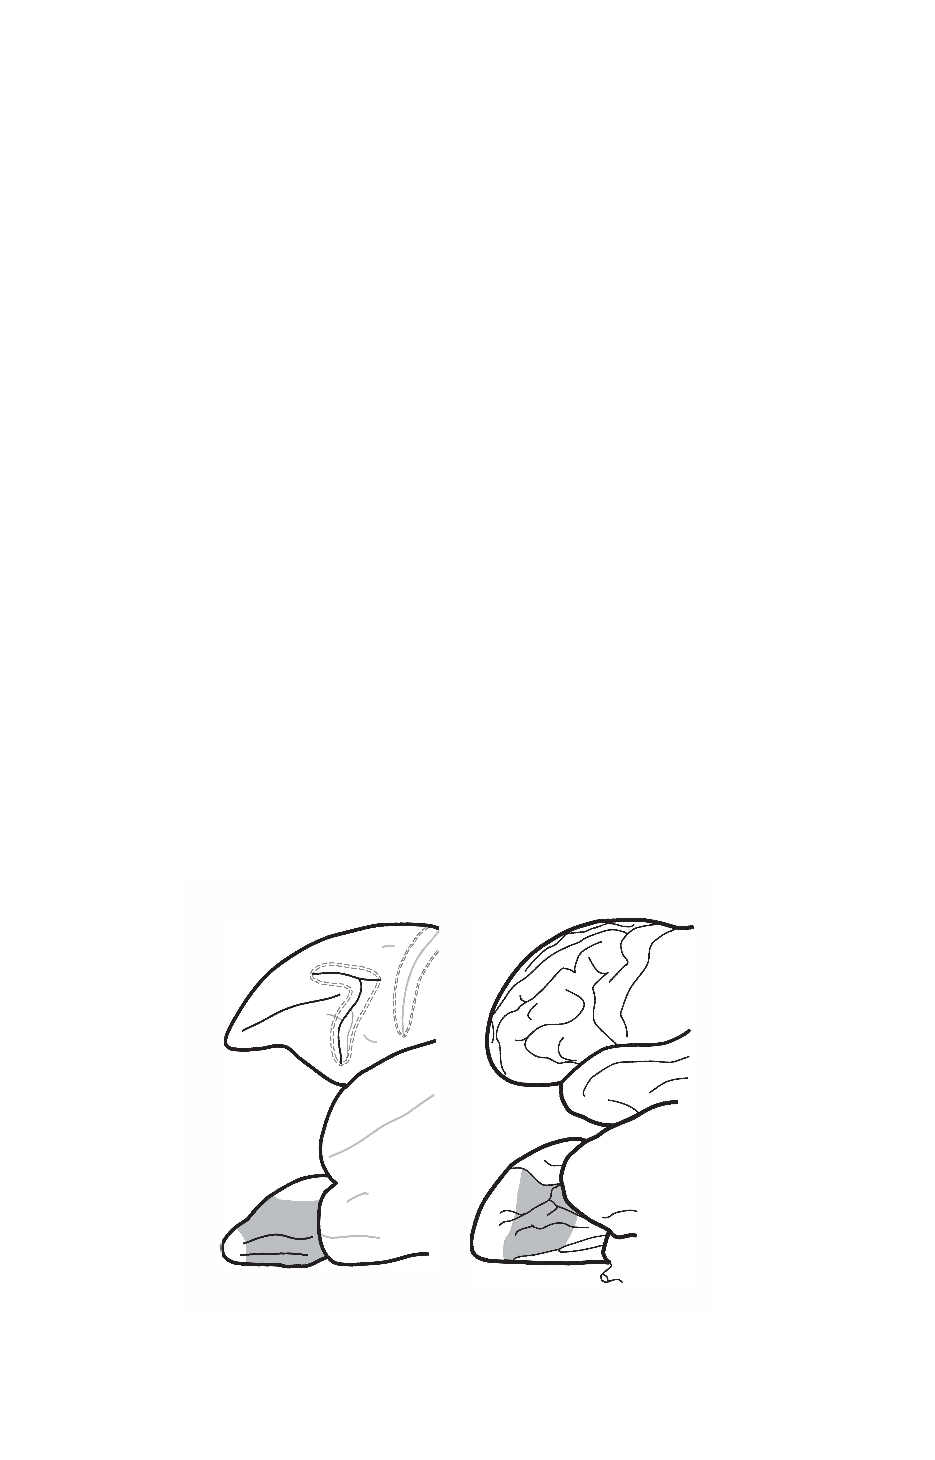
\includegraphics{chap4/fig_4_1}
	\caption{猴子(左)和人类(右)的眶额皮层。
		格式如图\ref{fig:1_2}所示。}\label{fig:fig_4_1}
\end{figure}



\section{连接}

图~\ref{fig:fig_4_2}~说明了眶额皮层的选定连接,这表明以下结论:\par


1. 与杏仁核最密集的连接涉及眶额皮层的颗粒部分,优先与杏仁核的基底外侧颗粒连接。
然而,13 区的颗粒状部分也与杏仁核有关,其他粒度细分(见图\ref{fig:3_3}
\cite{carmichael1995limbic}。\par


\begin{figure}[!htb]
	\centering
	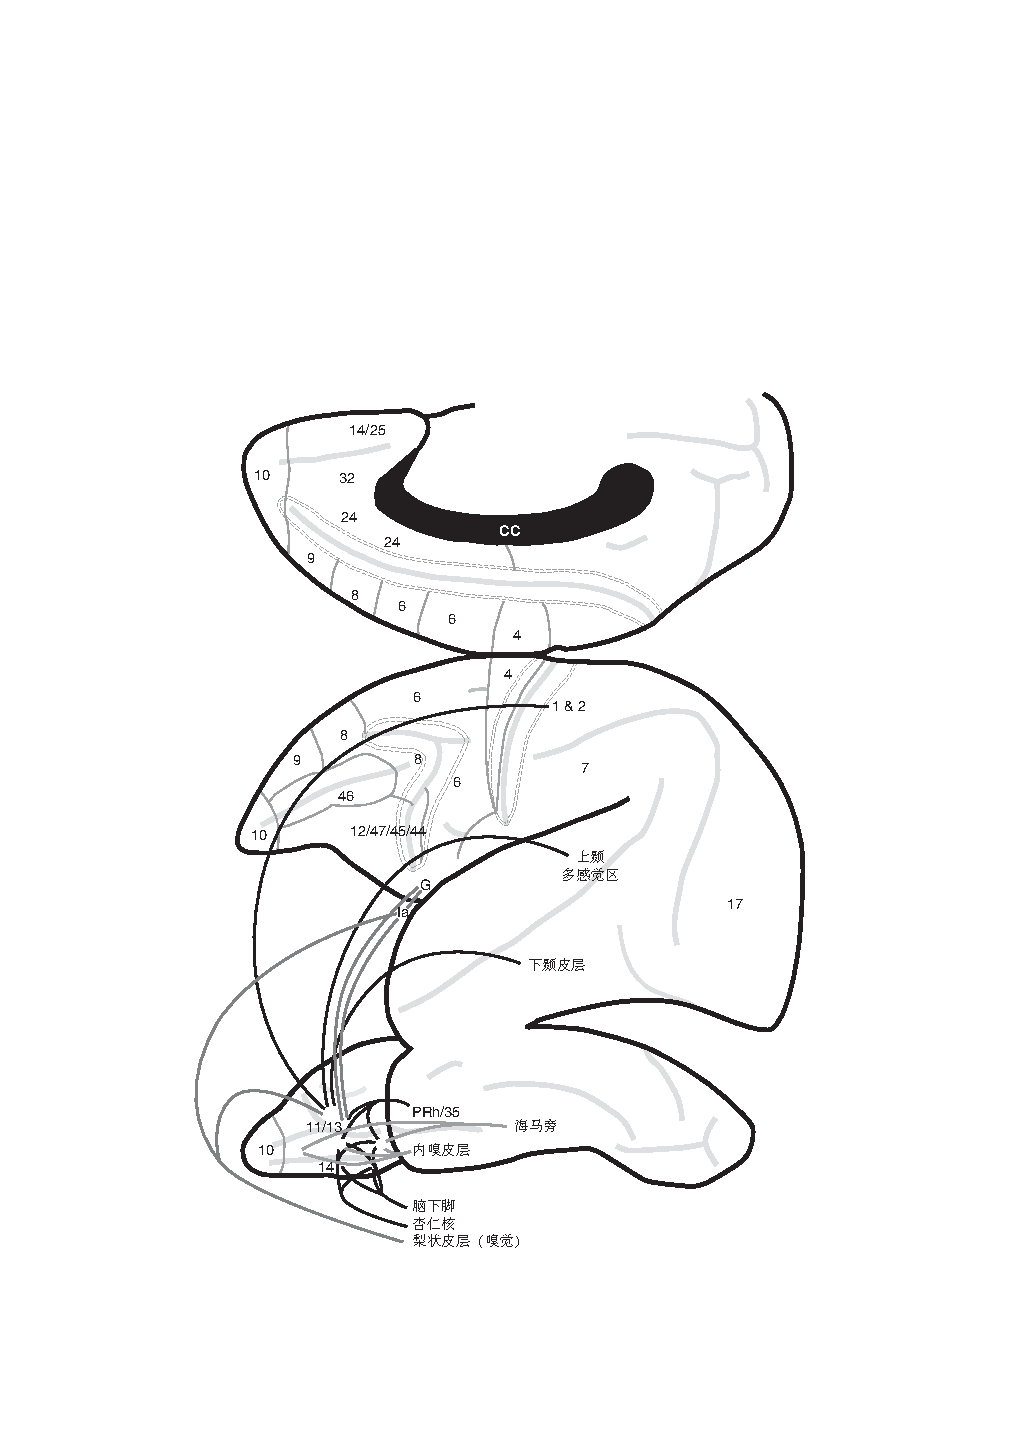
\includegraphics{chap4/fig_4_2}
	\caption{眶额皮层的选定连接。
		图~\ref{fig:1_4}~和~\ref{fig:1_5}~给出了脑沟和区域的名称。
		线连接一些与轨道有直接轴突连接的区域,除非另有说明,否则假设是相连的。}\label{fig:fig_4_2}
\end{figure}


2. 无颗粒岛叶皮层接收来自味觉和梨状(嗅觉)皮层\cite{carmichael1995sensory}。
它还接收来自脑干和丘脑的内脏信号\cite{ray1992organization}。
后者包括传达反映动物新陈代谢状态的信号的感觉,例如,缺氧或低血糖,以及来自肺、心脏、压力感受器和消化道\cite{craig2002you}。
这些发现导致了这样一种观点,即颗粒状岛叶皮层在内感受中发挥作用。\par


3. 嗅觉、味觉和内脏信息从其无颗粒部分到达颗粒状眶额皮层部分\cite{carmichael1994architectonic}。
该信息可以在颗粒皮层中与来自颞下皮层的视觉输入相结合,目标区域 13 和 11,以及从投射到区域 13 的鼻周皮层\cite{saleem2008complementary}。
后一种投射提供了关于物体的多模态信息\cite{murray2007orbitofrontal}。\par


4. S1区和S2区的体感信息也会传到13区,尤其是那些代表嘴侧\cite{pritchard1986projections}、唇和舌的侧面部分\cite{carmichael1994architectonic}。
这些联系包括不明确的体感诸如顶叶盖和岛叶颗粒异常部分的区域皮层\cite{saleem2008complementary},以及定义明确的体感区域,例如区域3b 和 S2 本身。
与 S2 的某些联系可能涉及手和口面部表征 分~\cite{carmichael1994architectonic}。\par


5. 与内侧前额叶皮层和腹侧前额叶皮层(第\ref{chap:chap3}章和第\ref{chap:chap7} 章)不同,眶额皮层只有有限的听觉输入~\cite{saleem2008complementary}。
14 区和 13 区的部分区域与颞叶中可能提供听觉输入的区域有联系\cite{petrides1996specialized}。
但是Saleem等人~\cite{saleem2008complementary}重新诠释这些连接是根据他们识别的两个连接网络来表示的:眶额网络和内侧网络。
他们认为与听觉相关的区域要么是内侧网络的一部分,要么是两个网络的一部分。
根据这种观点,眶额皮层的“纯眼眶”部分缺乏听觉输入。
原因大概是轨道网络处理有关物体(例如食物)的信息,这些物体几乎没有听觉特征。\par


这些点构成了眶额皮层的连接指纹,这表明它是视觉信息与味觉、嗅觉和内脏输入融合的最早部位。
我们认为大多数视觉输入到达很重要。在灵长类动物特有的颗粒状区域。
因此它不是眶额前额叶皮层,一般来说,但特别是区域 13 和 11 的颗粒状部分似乎是视觉、嗅觉、味觉和内脏输入之间会聚的最听觉位置。\par


由于这种融合,看到某种特定的食物,例如处于特定成熟阶段的水果,可以唤起它的味道和气味,这些味道和气味构成了它的味道,以及摄入后的内脏感觉。
此外,眶额皮层接收来自初级体感皮层的口、唇和舌表征的输入(S1):是与食物和液体摄入最相关的身体部位\cite{carmichael1995sensory}。\par


它的连接解剖结构使眶额皮层处于一个独特而有趣的位置。
触觉输入提供有关外部环境附近部分的信号;
视觉和嗅觉输入传递来自外部世界遥远部分的信号;
内脏输入告诉动物有关其内部环境的信息;
味觉和口腔体感输入告诉它有关从外部进入内部世界的事物。\par


图 \ref{fig:fig_4_3} 显示了这些不同的模态和子模态如何组合起来形成联合表征。
其中一些连接发生在无颗粒区域,它们似乎非常适合早期哺乳动物的谷物和昆虫饮食。
这些是专门从事夜间觅食以避免捕食等因素的小动物。
因此,在眶额前额叶皮层的颗粒部分中表示的连词主要涉及味觉、嗅觉和内脏感觉。
灵长类动物灵长类动物保留了这种基本的特征连接机制,并增加了更大的来自视觉区域的输入。\par


\begin{figure}[!htb]
	\centering
	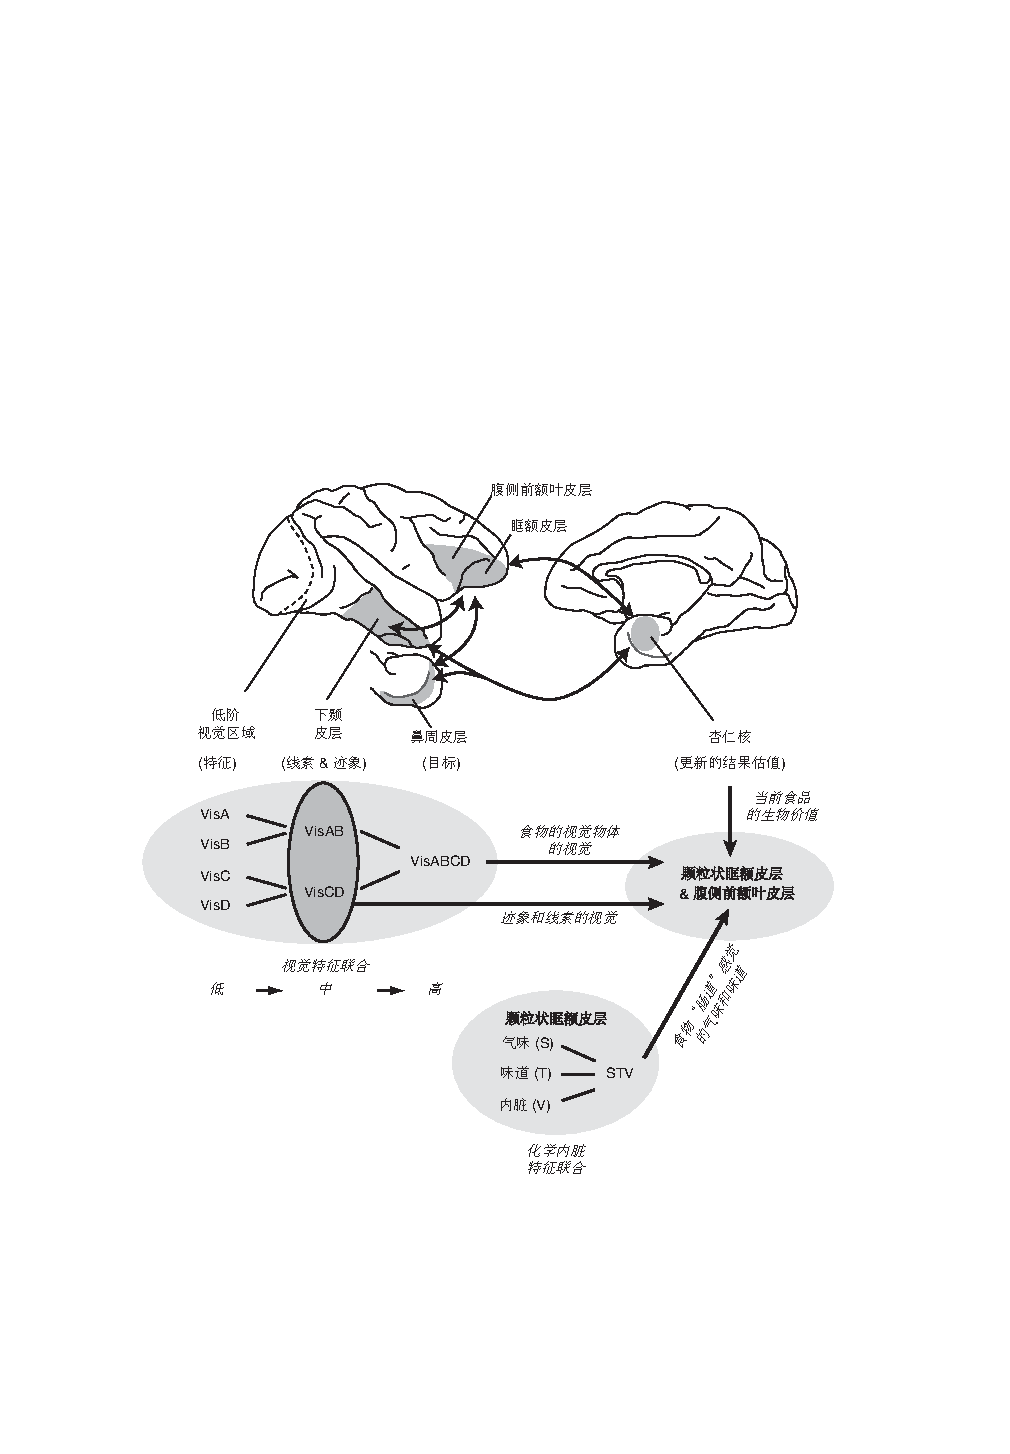
\includegraphics{chap4/fig_4_3}
	\caption{颞叶皮层和额叶皮层的特征连接。
		VisA …VisD 指定视觉
		对象的特征,可以组合成各种连接表示,例如 VisAB,
		这表示 VisA 和 VisB 的表示。 
		“STV”表示物体的气味 (S)、味道 (T) 和内脏 (V) 特性的结合\cite{murray2011can}。}\label{fig:fig_4_3}
\end{figure}



\subsection{概括}

第 \ref{chap:chap3} 章认为——通过与海马体、杏仁核和内侧运动前区的联系——内侧前额叶皮层会偏向于在动作之间或在动作之间的选择有关行动的规则。
在那里,我们审查了证据表明它是基于预测结果的当前值这样做的,尤其是当这些选择取决于“内部”信号而不是感官信号时。
本章认为眶额前额叶皮层执行在外部信号之间进行选择的类似功能,尤其是那些来自物体的信号。
它之所以能够这样做,是因为来自体感、味觉、嗅觉、内脏和视觉皮层以及杏仁核的信息会聚和整合。



\section{啮齿动物的无颗粒皮层}

无颗粒状前额叶皮层在啮齿动物研究中引起了相当大的关注,其中大部分表明在以结果为导向的行为中起着重要作用。
回想一下,在整本书中我们区分了目标和结果,因此在其他人可能会说目标导向的地方使用术语“结果导向”。
\textit{眶额皮层}细胞的活动反映了结果预测,尤其是关于奖励的特定感官方面的预测\cite{schoenbaum1998orbitofrontal},这些区域的损伤会损害基于结果预期的选择,如下一节所述。



\subsection{刺激-结果关联}

正如第 \ref{chap:chap3} 章提到的,当前的生物需求会影响结果的评估。
例如,当前对食物或液体的需求越大,对应该结果的刺激的价值就越大。
食用食物至饱足感会使该食物贬值,并且还有其他方法可以改变结果的价值。\par


在使用这些替代方法之一降低食物奖励价值的实验中,Gallagher等人\cite{gallagher1999orbitofrontal}把颗粒状前额叶皮层损伤的老鼠的行为与正常老鼠相比。
首先,他们教老鼠光表示食物供应。
当灯亮时,老鼠会靠近灯。
然后加拉格尔等人。
用过的锂氯化物诱发胃肠道疾病,这一过程称为条件性味觉厌恶。
稍后进行测试时,在所有疾病痕迹消失后,正常老鼠接近光的次数比患病前要少,或者完全停止接近光线。
受伤的老鼠表现不同。
它们比正常老鼠更频繁地接近光线。
正如第 \ref{chap:chap3} 章所解释的,正常老鼠的结果称为贬值效应。
因为受损的老鼠接近了与奖励贬值相关的刺激,所以可以说它们在利用刺激-结果关联来指导行动方面存在障碍。\par


Pickens等人\cite{pickens2005orbitofrontal,pickens2003different}使用相同的任务和贬值程序,但对杏仁核和无颗粒状眶额皮层造成损伤。
两个损伤都废除了老鼠的贬值效应。
这些老鼠的行为就好像它们没有从疾病上学到任何东西一样。\par


这些贬值程序的结果类似于第 \ref{chap:chap3} 章描述的结果对于内侧前额叶皮层的损伤。
内侧前额叶皮层损伤会导致使用结果预测来选择竞争行为的障碍。
在许多这样的实验中,没有任何外部提示可以帮助动物做出选择。
无颗粒状眶额皮层损伤不会破坏这种行动-结果关联\cite{ostlund2007orbitofrontal}。
相反,它们破坏了使用关于结果的预测来在对象中进行选择。
在这些实验中,外部提示会提示选择,从而揭示学习刺激与结果关联的缺陷。
这些研究表明,无颗粒状眶额皮层将刺激与结果联系起来,尤其是食物的感官方面,例如它的气味或味道。\par


伯克等人的一项实验( 2008 ) 支持这一结论。
老鼠首先学会了将一种刺激与一种特定的食物联系起来。 后来他们看到了这种刺激与额外刺激的结合。
当老鼠看到这种复合刺激时,它们得知它与另一种食物有关。
这两种食物的适口性和吸引力大致相同,但它们的味道不同。\par


伯克等人发现老鼠将第二种食物的发生归因于复合刺激的较新部分。
作为这一结论的证据,他们表明他们的老鼠会按下一根杆来产生额外的刺激。
至关重要的是,Burke等人表明如果老鼠对第二种食物感到满意,那么它们就不太可能这样做。
因此,老鼠不仅将额外的刺激与第二种食物联系起来,而且使用该关联来评估刺激的当前值。
具有无颗粒状眶额皮层损伤的老鼠未能显示出这些效果。
关系在复合刺激的较新部分和特定感觉特性之间第二种食物不再影响他们的行为。
这些结果表明无颗粒状眶额皮层介导刺激和结果之间的映射,尤其是结果的特定感官方面。\par


稍后,我们强调了颗粒状眶额皮层的重要性和灵长类动物视觉上的进步。
然而,正如刚才回顾的实验所表明的那样,老鼠也使用视觉评估结果的刺激,他们的眶额皮层从视觉皮层区域接收到这些刺激。\par



\subsection{费用}

第~\ref{chap:chap3}~章解释了动物不仅根据预测的食物或液体做出决定,而且还有获得它们的成本。
例如,与正常大鼠相比,前扣带回晚期皮层受损的大鼠选择越过障碍的次数较少,因此似乎高估努力成本。\par


无颗粒眶额皮层的损伤也改变了大鼠估计成本的方式。
当在立即的小奖赏和延迟的大奖赏之间做出选择时,正常老鼠在做出选择时会考虑延迟的时间长短。
Rudebeck等人\cite{rudebeck2006separate}报道有眶额皮层的大鼠更多地选择小的即时奖励经常比正常老鼠。
“冲动”一词已被应用于选择小额奖励很快,并且“耐心”一词已被用于放弃立即奖励以获得一个更大的以后。
所以在 Rudebeck 等人的实验中,眶额皮层眼眶病变可以据说会诱发冲动。\par


然而,只要稍微改变实验设计,就会得到不同的结果。
鲁德贝克等使用了 T 型迷宫,但 Winstanley 等人\cite{winstanley2004contrasting}让老鼠在两个杠杆之间进行选择,一个导致单个颗粒,另一个在延迟后导致四个颗粒。
眶额皮层病变的大鼠比正常大鼠更频繁地选择延迟奖励的杠杆。
有人可能会说他们表现出比正常人更多的“耐心”。
和Mariano等人\cite{mariano2009impulsive}让老鼠在 T 迷宫上的黑色或白色目标框之间做出选择,一个框内有小奖励,另一个框内有大量奖励,只有在延迟后才能获得。
同样,患有眶额皮层病变的大鼠比 Rudebeck 等人研究中的大鼠表现出更多的“耐心”。\par


泽布等人\cite{zeeb2010contributions}表明,眶额皮层病变是否会导致“冲动”或“患者”选择取决于两个因素:
一个明确的信号,表明个体大鼠之间的延迟和差异。
他们使眶额皮层失活并比较了提示的效果和无意识的延误。
他们的结果表明,对于明显有提示的延迟,失活会增加立即奖励的选择(冲动),而对于无提示的延迟,失活会减少立即奖励的选择(耐心),但仅限于有强烈冲动倾向的老鼠个体。
所以我们不能简单地说大鼠眶额皮层偏向于冲动或耐心觅食的选择。
但是,它显然以某种方式在评估延迟成本方面发挥了作用以及偏向延迟或立即行动的行为。
正如第 \ref{chap:chap3} 章所解释的那样,累加器-跑道模型提供了一种实现这种偏差的简单机制,既可以通过改变产生输出的阈值,也可以通过调制速率支持进行特定运动的“证据”不断积累. \par


冲动觅食和耐心觅食之间的竞争通常是根据延迟或远距离获得的食物和液体的贬值或折扣来讨论的。
然而,正如斯蒂芬斯等人\cite{stephens2004impulsiveness}指出,这个术语意味着动物错误地评估了时间和空间上遥远的食物和液体的价值。
或者,动物可能会准确评估价值,但会考虑寻找遥远可用资源的固有风险。 \par


Hayden\cite{hayden2007temporal}建立了一个模型,其中“风险”期权的估值取决于较大收益的预期时间和收益减少的风险。
他们表明,该模型的预测解释了猴子在赌博任务中做出的选择。
由于等待更长时间或走得更远所固有的风险,选择开发立即可用的资源并不一定意味着对延迟或更远资源的错误评估。
即使眼前的补丁比别处的“更绿的牧场”价值低,回报更确定。



\subsection{颗粒状岛叶皮层}

基于连接、细胞结构和拓扑结构,眶额皮层包括无颗粒岛叶皮层\cite{carmichael1994architectonic}。
如果无颗粒眶额皮层将刺激与结果的特定感觉方面相关联,我们可能期望找到邻近的无颗粒岛叶皮层的相关功能。
Balleine\cite{balleine2000effect}表明,具有包括无颗粒岛叶皮层在内的损伤的大鼠在需要记住特定味道时表现出损伤。
他们在两种情况下对老鼠进行了测试。
在其中一项中,老鼠在两个杠杆之间做出选择,并接受了那种与任一选择相关的食物。
受损的老鼠倾向于避免按下刚刚导致奖励贬值的杠杆。
在第二种情况下,压榨机不再生产任何食物;
也就是说,老鼠在灭绝中进行了测试。
在这种情况下,受伤的老鼠同样地按下了两个杠杆。\par


因为其他实验表明有这些损伤的老鼠可以学习这种消退任务,Balleine 和 Dickenson 得出结论,有损伤的老鼠无法回忆起它们期望通过按下每个杠杆获得的食物的特定感官特性,因此,尽管其中一种食品贬值,但他们同样选择了它们。
尽管他们的病变侵入了位于岛叶皮层尾侧的味觉皮层,但这种影响可能是由岛叶皮层病变引起的。\par


Kesner\cite{kesner2007role}还测试了老鼠预期奖赏的能力。
老鼠先喝低蔗糖液体,然后喝高蔗糖液体,几天后,它们喝的低蔗糖液体减少了,以便以后消耗更多的高蔗糖液体。
无颗粒岛叶皮层的损伤消除了这种效应。
然而对照试验表明,受损的大鼠仍然可以分辨出两种液体之间的差异。
本实验表明,岛叶皮层受损的大鼠倾向于选择即时奖励,而不是等待更高价值但延迟的奖励。
这结果可能反映出未能预测延迟奖励的属性或冲动的选择。\par



\subsection{概括}

按照本章第 \ref{chap:chap3} 章所述,颗粒状内侧前额叶皮层似乎使用行动-结果映射和动机评估来偏向行动或有关行动的规则之间的选择。
映射和估值都涉及“内部”信号,两者都可以影响代表特定选择的累加器网络中的活动(第~\ref{chap:chap3}~章)。
因此,例如,按下杠杆预测有益结果(例如葡萄干)的“内部”信号以及评估该结果的信号就当前需求而言,两者都为代表压杆行为的累加器网络提供了“证据”。
有了更多这样的“证据”——例如,更强的关联或获得葡萄干的更高动机——网络将更快地达到阈值并“赢得”控制行为的“竞赛”。
相比之下,眶额皮层的颗粒部分似乎使用刺激-结果映射以及动机评估来偏向刺激之间的选择。
与行动-结果映射不同,刺激-结果映射依赖于外部的、感官的信号以及内部信号(关于动机),它们也可以影响累加器网络中的活动。
因为这些区域通过它们密集的互连一起工作\cite{barbas1988anatomic,price2010neurocircuitry},它们允许哺乳动物选择预测最佳结果的行动或刺激,根据当前的动机价值更新。
我们认为,这种能力比缺乏这些皮层区域的祖先物种更具优势(第~\ref{chap:chap2}~章)。
由于它们的无颗粒眶额皮层,哺乳动物可以在面对不断变化的环境时迅速改变觅食选择。
上一章表明,他们可以学习习惯应该盛行或以结果为导向的行为应该盛行的环境,他们可以学习何时应该通过内在或外在规则来引导导航,并且他们可以通过努力来权衡奖励收益费用。
本章表明他们可以了解“冲动”或“耐心”觅食的背景。
从这个意义上讲,哺乳动物可以获得相互矛盾的行为知识,当环境发生变化时,它们可以用来偏向其他行为控制系统。
第~\ref{chap:chap3}~章解释了这如何在神经网络层面发挥作用。
表~\ref{tab:tab_4_1}~总结了这些与觅食选择相关的想法。
它并不意味着详尽无遗。
例如,我们忽略了巴甫洛夫到工具的转移、差异结果效应和条件强化等现象。
啮齿动物的颗粒状眶额皮层损伤会导致这些任务以及本章和表~\ref{tab:tab_4_1}~强调的任务受损。



\begin{table}[htbp]
	\newcommand{\tabincell}[2]{\begin{tabular}{@{}#1@{}}#2\end{tabular}} %换行指令
	\centering
	\caption{颗粒状眶额皮层对觅食选择的贡献}
	\renewcommand\arraystretch{1.5}	%设置表格内行间距
	\begin{tabular}{llll}
		\toprule 
		区域   &  贡献  \\
		\midrule
		\tabincell{c}{内侧颗粒状眶额皮层\\}&根据预测的成本/收益,在多种行动选择中偏向觅食\\&在中等波动环境中偏向于以结果为导向的选择\\&偏向低波动环境的习惯觅食\\&偏向于外在或内在的导航规则\\
		\midrule
		\tabincell{c}{颗粒状眶额皮层}&基于结果的预测感官方面的多种刺激之间的偏差觅食\\&偏向于“冲动”觅食以利用可用资源\\&偏向“耐心”觅食以探索遥远的资源 \\ 
		\bottomrule
	\end{tabular}%
\label{tab:tab_4_1}
\end{table}%



\section{灵长类动物的颗粒区域}

第 \ref{chap:chap2} 章和第 \ref{chap:chap3} 章讨论了啮齿动物的内侧额叶皮层与灵长类动物的中外侧前额叶皮层(46 区)同源或类似的说法。
没有令人信服的证据支持这一建议,很多人反对。
在这里我们简要地处理一个关于眶额皮层的相关争论。\par



\subsection{比较啮齿动物和灵长类动物的颗粒区域}

与灵长类动物的眶额皮层不同,大鼠的眶额皮层完全没有颗粒。
此外,它具有非常类似于颗粒状但不是颗粒状的连接,部分灵长类眶额皮层。
与粒状前额叶皮层不同,它位于异质皮层附近,并且与粒状前额叶皮层不同,它对自主输出有相对直接的影响。\par


然而,尽管有所有这些证据,一些神经科学家认为大鼠的颗粒状眶额皮层对应于猴子的整个眶额皮层,包括其颗粒区域\cite{uylings2003rats,seamans2008comparing,schoenbaum2009new}。
第 \ref{chap:chap2} 章解释了这个想法采用两种形式之一。
一是老鼠有猴子眶额皮层的微型复制品;
另一个是他们融合了所有领域发生在猴子身上。
这两种观点都基于大鼠和猴子眶额皮层之间的某些相似性,例如细胞活动、神经化学特性、连接和损伤效应。
但是所引用的相似性并不对应于诊断特征,而诊断特征正是建立同源性所需要的。
正如第 \ref{chap:chap2} 章和第 \ref{chap:chap3} 章所讨论的,诊断特征将不同的区域区分开来。
以条件反射的消失为例。
尽管有眶额皮层,损伤的大鼠表现出比正常消退慢\cite{kolb1974double},但猴子中仅限于颗粒状眶额皮层的损伤具有相同的效果\cite{izquierdo2005comparison}(图~\ref{fig:fig_4_4}),包括颗粒状眶额皮层损伤也是如此 猴子\cite{butter1969perseveration}。
因此,有问题的相似性——称为眶额皮层的区域的病变导致灭绝学习减慢——无助于我们建立同源性。\par


\begin{figure}[!htb]
	\centering
	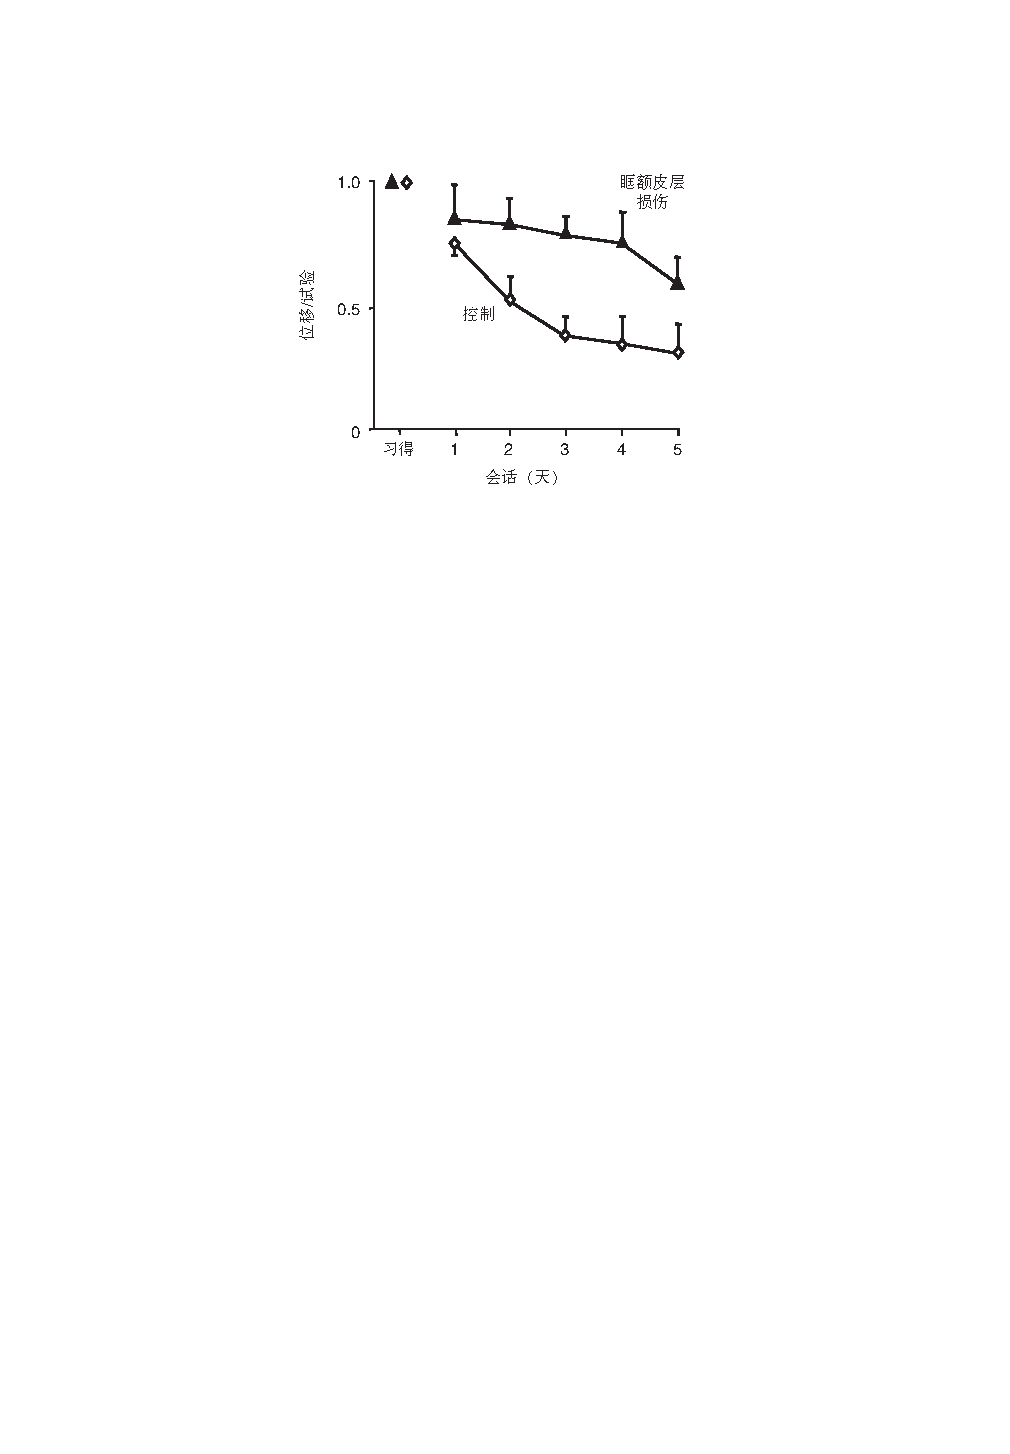
\includegraphics{chap4/fig_4_4}
	\caption{猴子颗粒状\textit{眶额皮层}损伤导致的消退学习减慢。
		猴子优先学习移动物体以获得食物奖励。
		在这个习得阶段,猴子在每次试验中有 30 秒的时间来移动物体,而且它们在每次试验中都会这样做。
		在随后的测试阶段,称为消弱试验,取代该物体永远不会产生食物。
		正常(对照)猴子将他们的位移减少到试验的一半以下5天的测试。
		具有颗粒状\textit{眶额皮层}损伤的猴子以高于正常的猴子,尽管经过 5 天的测试后它们有了显着改善\cite{izquierdo2005opposing}。}\label{fig:fig_4_4}
\end{figure}



\subsection{细胞活性}

不幸的是,除了我们之前回顾的解剖学知识外,我们对灵长类动物眶额皮层的颗粒部分知之甚少。\par


罗尔斯等人\cite{rolls1994emotion}]记录了眶额皮层中对咸味、苦味、酸味和涩味做出反应的细胞。
从我们对它们记录位置的检查来看,它们似乎主要记录了 13 区和 14 区的颗粒部分,在 13 区的颗粒部分和岛叶皮层的颗粒部分也有额外的细胞群。
所有这些区域的细胞都会对口味做出反应。\par


除了味觉输入,视觉和嗅觉输入有助于确定食物和液体的特性。
在 Rolls 和 Baylis 的研究中,眶额皮层中的细胞对视觉和味觉的结合以及嗅觉和味觉的结合都有反应。
大多数显示味觉-视觉或嗅觉-视觉连接的细胞发生在眶额皮层的尾侧。
一些位于岛叶皮层的颗粒状区域,而另一些位于 13 区的颗粒状部分或至少附近。
相同的特性发生得更多也位于眶额皮层。\par


Rolls 和他的同事还发现,猴子会按下一个杠杆,通过电极刺激第 13 区的颗粒状部分,这表明它们发现这种刺激是有益的\cite{mora1980electrophysiological}。
刺激 11 区没有这种效果。
所以细胞位于眶额皮层更靠后的部分,包括那些对味觉或视觉或气味与味觉的结合有反应的部分,似乎与大脑其他部位的奖赏系统的相互作用比眶额皮层的更靠侧部分更直接。\par



\subsection{概括}

啮齿类动物和灵长类动物都有一个无颗粒的眶额皮层(见图 \ref{fig:fig_2_1}),我们假设它的某些功能是从它们的共同祖先那里继承而来的。
不幸的是,我们几乎没有关于猴子眼眶无颗粒区域的直接损伤或细胞记录证据,因此我们承认这只不过是一种假设。
然而,我们确实知道颗粒区域具有密集的互连与颗粒区域,并且颗粒区域中的细胞具有我们在此基础上期望的感觉反应,例如用于识别特定食物和液体的视觉,气味和味道的结合。
当然,在实验室中,这些食物和液体可作为指导行为的结果。\par



\section{颗粒状皮层}

与灵长类动物中颗粒状眶额皮层的信息匮乏相比,其颗粒部分已得到广泛研究。
我们根据损伤对刺激和结果之间的关联映射的影响、神经编码这些映射根据特定结果和“通用货币”、基于结果的规则选择、对这些结果的动机估值的更新以及将结果准确分配给选择。



\subsection{刺激-结果映射}

与其他动物一样,猴子使用刺激来预测结果并在此基础上做出觅食选择。
两种实验证明了这些预测:概率结果实验(图~\ref{fig:fig_4_5}B)和确定性结果实验(图~\ref{fig:fig_4_5}A)。
在前者中,猴子选择两种或多种产生奖励概率不同的刺激中的一种;
在后者中,猴子学会在两种刺激之间做出选择,以始终获得奖励,并在奖励偶然性切换到替代选择时改变选择。\par


\begin{figure}[!htb]
	\centering
	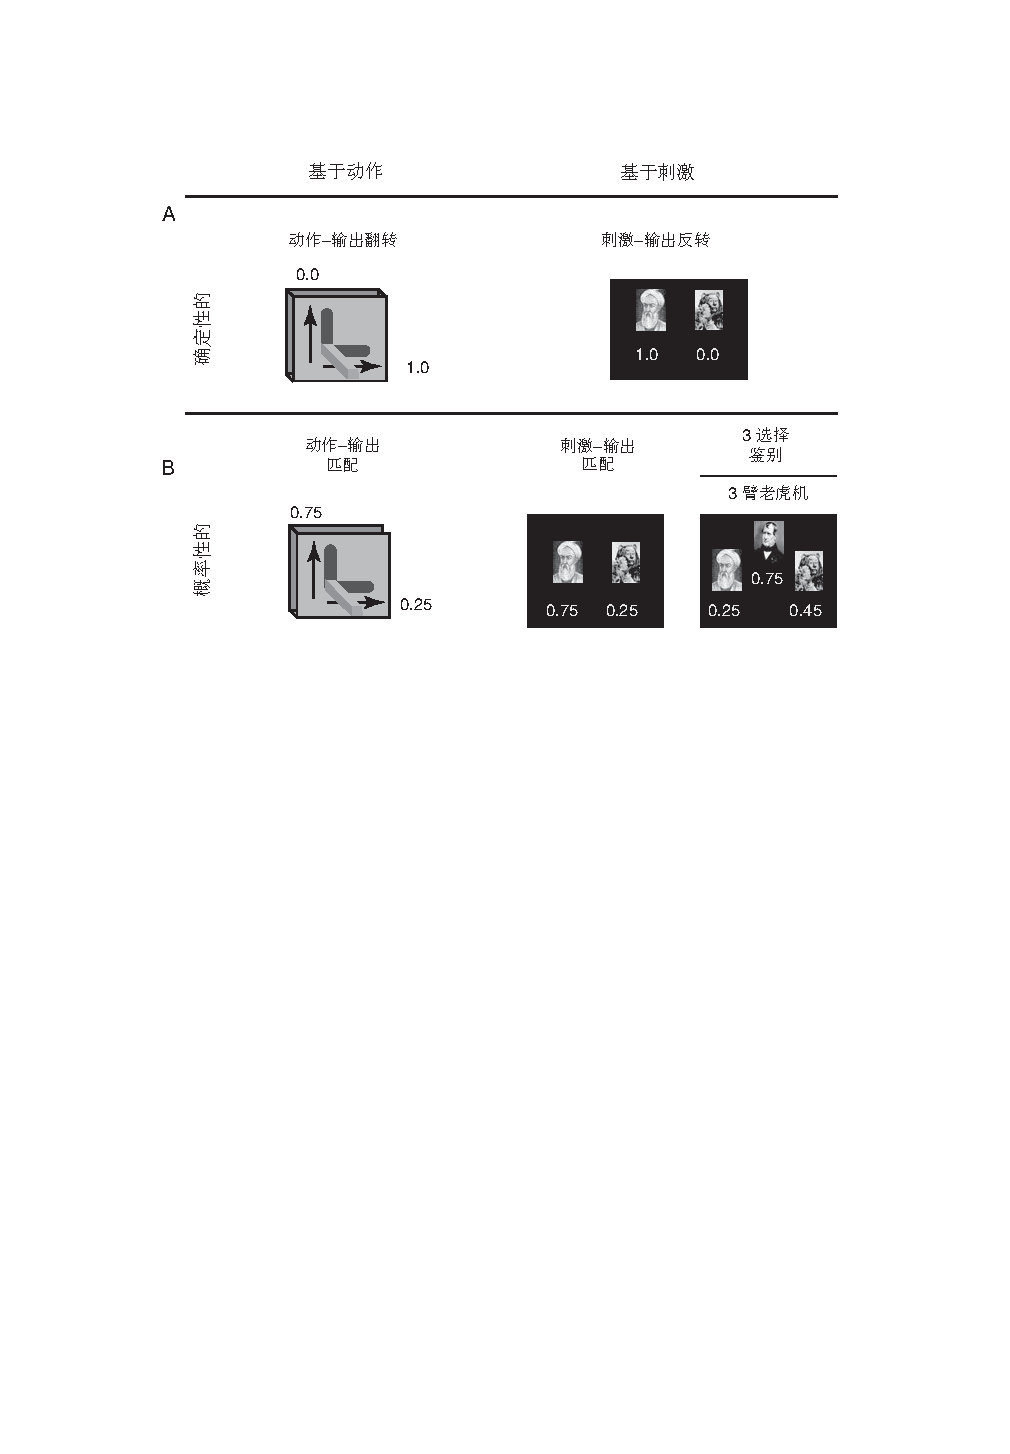
\includegraphics{chap4/fig_4_5}
	\caption{区分基于动作(左)和基于刺激(右)选择的实验。
		(一) 在
		基于确定性动作的选择(左),将手柄向右移动被描述为导致
		每次奖励,比例为1.0,而向上移动手柄永远不会产生奖励(0.0)。
		这些结果后来在确定性动作逆转任务中切换。
		对于基于刺激的选择(右),猴子必须接触触摸屏上显示的两张图片之一。
		每个选择的奖励概率是确定性的(0.0 或 1.0)。 
		(B) 在概率任务中,对于两个动作之间的选择,奖励的可能性在 0 和 1之间变化(左)或两个物体(中间)。
		这些数字给出了每个选择获得奖励的试验比例。
		这些任务根据“匹配法则”称为匹配任务,而不是匹配样本任务。
		在三选择辨别任务(右)中,也称为三臂强盗任务,三种选择中的每一种都以不同的概率得到回报,这种概率随时间而变化\cite{rudebeck2008frontal}。}
	\label{fig:fig_4_5}
\end{figure}


鲁德贝克等人\cite{rudebeck2008frontal}使用概率方法。
在任务的一个版本中,称为刺激-结果匹配(图~\ref{fig:fig_4_5}B),他们分配了四个概率级别,两个独立的概率算法确定两个刺激中每个刺激的级别。
一次该算法为刺激分配了一个概率,该概率在试验中保持不变,直到猴子选择了该刺激。
然后概率发生了变化,因此动物不得不根据它们的概率在刺激选择之间反复切换付清。
在另一个概率任务中,称为三臂强盗任务或三选择辨别任务,猴子学会在三种刺激中进行选择,每种刺激的奖励概率随试验次数而变化(图~\ref{fig:fig_4_5}B)。\par


鲁德贝克等在受过训练以执行三臂强盗任务的猴子的颗粒状眶额皮层中造成损伤。
这些猴子调整他们的选择以改变奖励概率比正常猴子慢得多,这表明存在缺陷学习刺激和结果之间的关联映射(图~\ref{fig:fig_4_6})。
或者,我们可以根据学习(或更新)选择和结果之间的关联映射来描述损伤。
在本章的其余部分,我们交替使用刺激-结果、对象-结果和选择-结果。\par


然而,当这些猴子通过选择两种行为中的一种而不是通过选择两种刺激中的一种来获得奖励时,它们表现正常。
该任务要求猴子选择抬起或转动杠杆以获得奖励,这是确定性动作逆转任务的概率版本第~\ref{chap:chap3}~章介绍。\par


除了患有颗粒状眶额皮层损伤的猴子,Rudebeck 等人在刺激-结果匹配任务中测试了前扣带回皮层损伤的 mon 键。
他们发现在这些内侧眶额皮层损伤后刺激之间的转换没有受损,尽管 Kennerley 等人\cite{kennerley2006optimal}表明,相同的病变会损害动作之间的切换。\par



鲁德贝克等得出的结论是,内侧前额叶皮层支持动作和结果之间的关联映射,而眶额皮层介导刺激和结果之间的关联映射。
但是 Rudebeck 等人和肯纳利等人报告了局限于前扣带回沟的皮层病变的 ed 结果。
对于较大的病变,尤其是那些同时包括前扣带回和前扣带回的病变,会出现更加复杂的情况。
E. A. Murray 等人(个人通讯)据报道,在这些较大的病变后,猴子在标准物体逆转任务中有损伤。
然而,Meunier 等人\cite{meunier1997effects}直接比较了有扣带回和眶额皮层病变的猴子的表现,有眶额皮层病变的猴子在物体反转任务上犯了两倍的错误。  \par


因此,物体反转任务继续对理解眶额皮层产生重大影响。
图~\ref{fig:fig_4_5}A~说明了这个确定性任务。
当发生反转时,奖励偶然性在两种刺激之间切换,通常除了奖励或非奖励反馈外没有任何其他提示。\par


在一项早期且有影响力的研究中,Butter\cite{butters1969retention}对猴子进行了三项任务测试:对象反转学习、空间反转学习和消退。
在一些猴子身上,他去除了眶额皮层,连同位于眼眶表面的 12/47 区部分半球的。
这些猴子在对象反转学习和消退学习上有障碍,但在空间反转学习上没有。
在其他猴子身上,他移除了腹侧前额叶皮层,包括整个 12/47 区。
这些猴子在灭绝任务。\par


许多随后的实验已经证实了眶额皮层和腹侧前额叶皮层之间的功能区别,以及在眶额皮层损伤后对象反转和消退学习的缺陷\cite{dias1997dissociable,izquierdo2004bilateral}。
例如,腹侧前额叶皮层的损伤会在对象反向学习的初始阶段损害表现,但前额叶皮层损伤会导致更严重和更持久的损伤\cite{rygula2010differential}。\par


Butter 得出结论,眶额皮层的损伤会导致持续的行为障碍。
而且,从那时起,许多关于眶额皮层的研究都被解释为坚持、反应抑制和行为抑制\cite{roberts2000inhibitory}。
根据这个想法,有缺陷的猴子在抑制先前获得奖励的选择方面存在缺陷,这会产生毅力。\par


Rudebeck\cite{rudebeck2008frontal}重新审视了这个话题,他们从几个方面进行了分析。
首先,在图~\ref{fig:fig_4_7}~所示的数据分析中,来自 Izquierdo 等人\cite{izquierdo2004bilateral},他们计算了错误的总数,直到猴子完成了从选择先前奖励刺激到选择当前奖励刺激的转换。
正如预期的那样,Rudebeck 和 Murray 发现,双侧病变的猴子与正常猴子相比,眶额皮层在两个物体之间的选择更慢。
此外,与正常猴子不同,如果对一系列逆转进行测试,则受损猴子无法通过这一系列对象逆转测试进行改进(图~\ref{fig:fig_4_7})。\par


接下来,Rudebeck 和 Murray 逐个试验地分析了他们的结果,而不是像神经心理学家传统上所做的那样对试验块进行平均。
肯纳利等人\cite{kennerley2006optimal}他们对内侧前额叶皮层的动作逆转实验使用了相同类型的分析(第~\ref{chap:chap3}~章)。
Rudebeck 和 Murray 以两种方式测量了错误的数量,这两种方式都发生在刺激-结果映射发生逆转之后。\par


首先,如图~\ref{fig:fig_4_8}A~所示,Rudebeck 和 Murray 计算了第一个正确选择之前的错误数量,并将这些数据与第一个正确选择之后的错误数量进行了比较。
正常猴子和受损猴子之间的最大差异发生在第一次正确选择之后。\par


其次,如图~\ref{fig:fig_4_8}B~所示,作者研究了动物坚持正确反应的可能性有多大,作为最近奖励的函数,这是一种积极的反馈。
为此,Rudebeck 和 Murray 比较了一次试验后的性能错误,在错误纠正序列之后进行一次试验,在错误纠正序列之后进行一次试验,等等。
图~\ref{fig:fig_4_8}B~显示眶额皮层的损伤导致使用正反馈的效率低下。
即使两个、三个或四个正确(并获得奖励)在错误之后做出反应,患有眶额皮层损伤的猴子比正常猴子犯了更多的错误。
然而,他们的表现几乎正常,以回应来自无回报选择的负面反馈\cite{rudebeck2008frontal}克拉克等人。
( 2008 ) 在狨猴中发现了类似的结果。\par


结合 Kennerley 等人的类似分析\cite{kennerley2006optimal}。
对于行动-结果学习,Rudebeck 和 Murray 的结果为解离提供了进一步的支持内侧前额叶皮层和眶额皮层之间的功能。
在图~\ref{fig:fig_4_5}~所示的任务系列中,眶额皮层的损伤导致学习改变的刺激-结果关联的障碍,但不影响改变的动作-结果协会。
相比之下,内侧前额叶皮层的损伤——更具体地说是前扣带回皮层的损伤——会导致学习改变的动作-输出映射的损伤,对学习刺激-结果的影响较小且不太可靠映射。\par


最近一项针对人类的病变研究得出了类似的结论。
卡米尔等人\cite{camille2011double}研究了背侧前扣带皮层或前额叶皮层病变的患者。
对于后者,在颗粒状眶额皮层中发现了最大的重叠区域,靠近它与颗粒状眶额皮层的边界。
但在大多数患者中,病变涉及两个区域。
卡米尔等人。 使用与猴子实验相同的分析并发现相似的结果。
在刺激-结果任务中,受试者在一副彩色扑克牌中做出选择,这些扑克牌要么产生收益,要么损失 50 美元的游戏币。
一种颜色的一副牌在 86\% 的试验中获得收益,而另一种颜色在 14\% 的试验中获得收益。
在行动-结果任务中,受试者在前臂的旋前和旋后运动之间进行选择,结果相同。
科目后学会了正确的选择,意外事件就发生了逆转,就像在猴子实验中进行的行动逆转和对象逆转一样。\par


卡米尔等人测量了受试者在积极反馈后错误地改变了他们的选择的试验比例。
这种转变是错误的,因为反馈表明他们应该坚持之前的选择。
眶额皮层病变导致刺激-结果逆转受损,但这些患者在动作-结果任务中表现得像对照受试者(图~\ref{fig:fig_4_9})。
相比之下,与对照组相比,前扣带皮层损伤导致了行动-结果逆转的损害。
患有这些病变的患者在刺激-结果任务中也比对照组犯了更多的错误,但这种差异没有达到统计学意义(图~\ref{fig:fig_4_9})。\par


\begin{figure}[!htb]
	\centering
	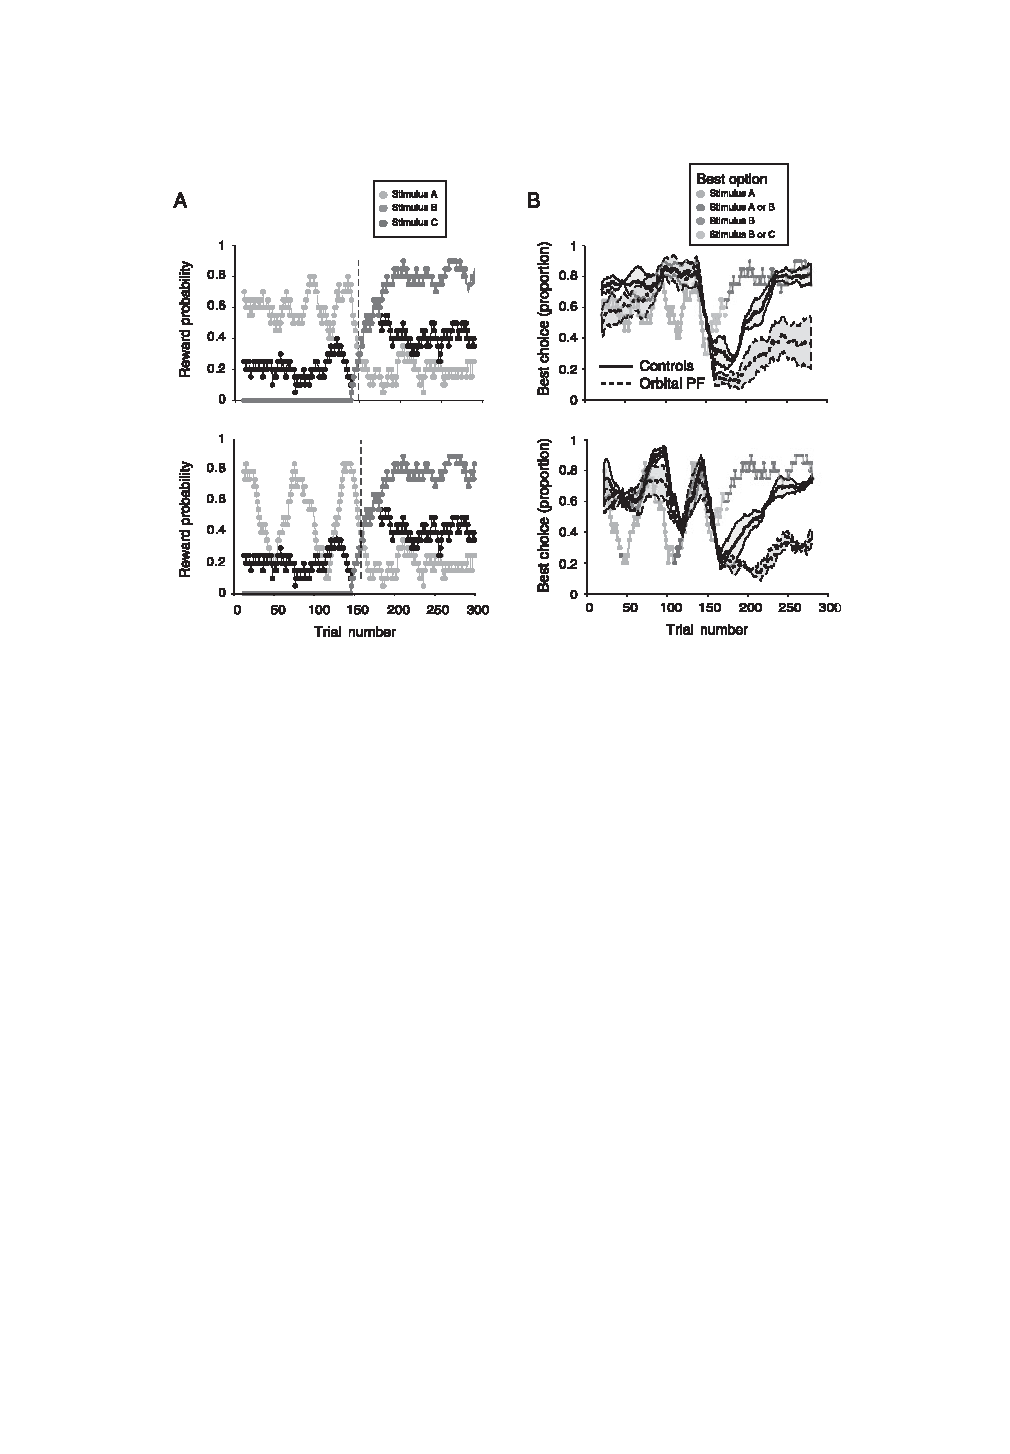
\includegraphics{chap4/fig_4_6}
	\caption{猴子颗粒状眶额皮层损伤后选择结果学习受损。
		(A) 对于图中说明的任务,选择三个类对象刺激中的每一个的回报概率图 4.5 右下角,三臂老虎机任务。
		回报率随试验的变化而变化数量,但不取决于猴子的选择。
		(B) 猴子的试验比例根据收益概率评估做出最佳选择。 纵坐标表示正常(对照)猴子(实线)选择最高价值对象(最佳选择)的比例和有颗粒状眶额皮层损伤的猴子(虚线)。
		阴影:SEM。
		任何试验中最佳刺激的回报概率以灰色绘制。
		顶行:低波动性条件。
		底部行:高波动情况\cite{walton2010separable}。}
	\label{fig:fig_4_6}
\end{figure}


\begin{figure}[!htb]
	\centering
	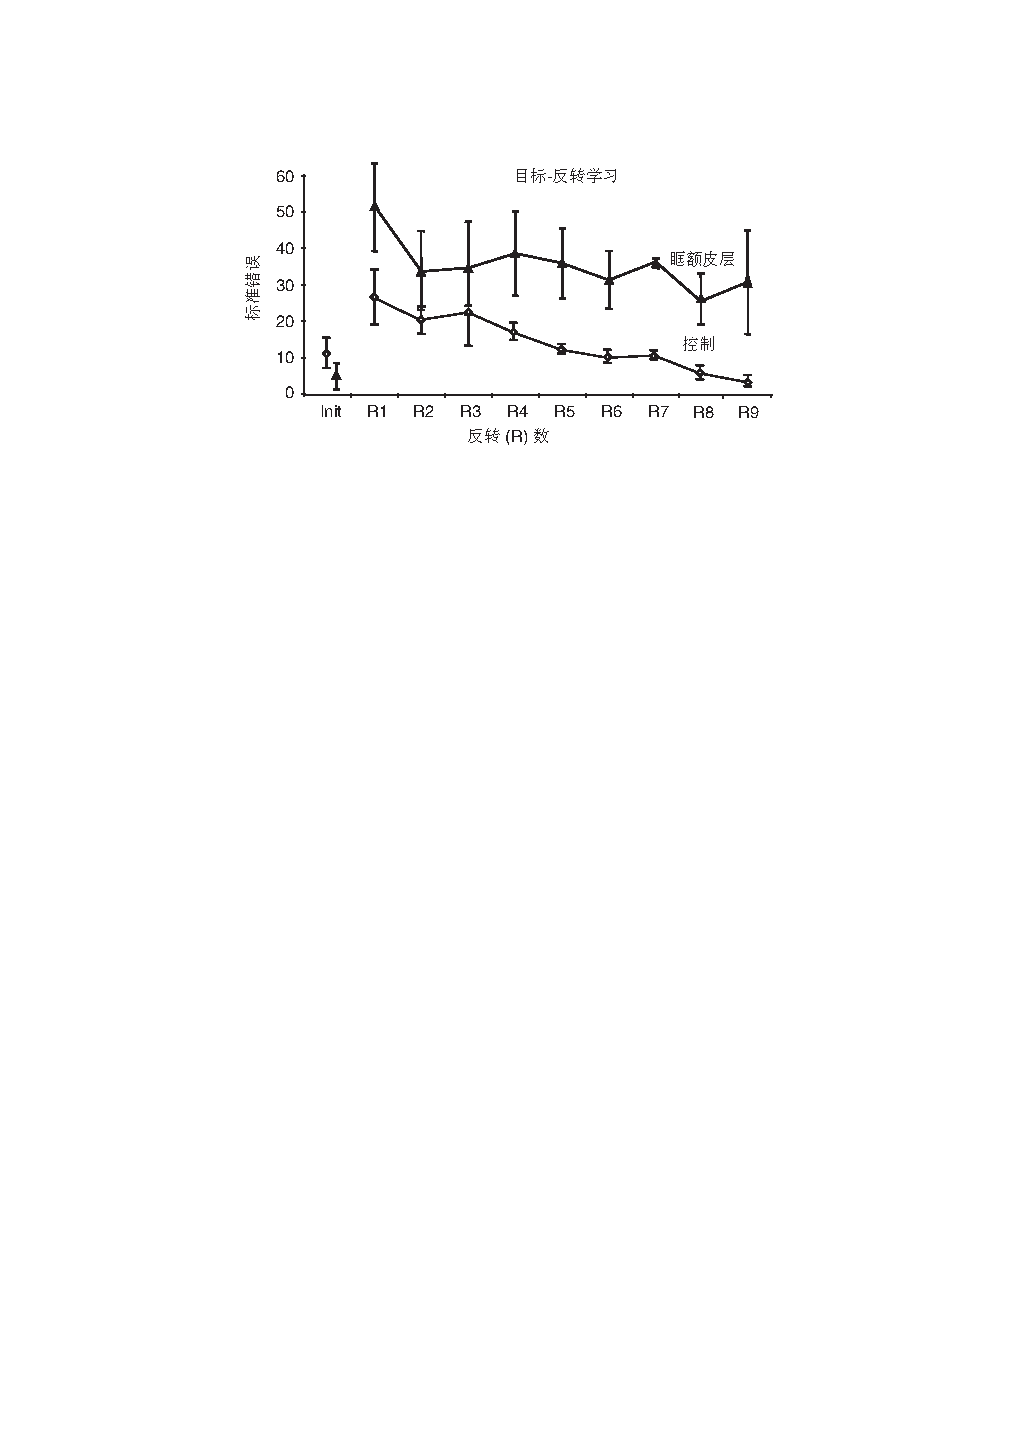
\includegraphics{chap4/fig_4_7}
	\caption{颗粒状眶额皮层损伤后猴子的物体逆转功能受损。
		数字错误标准性能的两个选择,确定性对象辨别任务。
		在初始训练(Init),没有逆转,猴子学会区分两个物体错误相对较少。
		眶额皮层在这种学习中不起作用,因为猴子只需要学习哪些对象是正值的,哪些是中性的。
		一旦简单将物体分类为阳性或中性不再解决问题,因此眶额皮层变得必要。
		R1. . R9 表示九个连续反转,其中随着时间的推移两个对象在交替的试验块中变得积极和中立。
		有颗粒状病变的猴子眶额皮层学习这些逆转的速度比正常(对照)猴子慢,而且它们无法改善连续九次逆转。
		误差线:SEM\cite{izquierdo2004bilateral}。}
	\label{fig:fig_4_7}
\end{figure}


\begin{figure}[!htb]
	\centering
	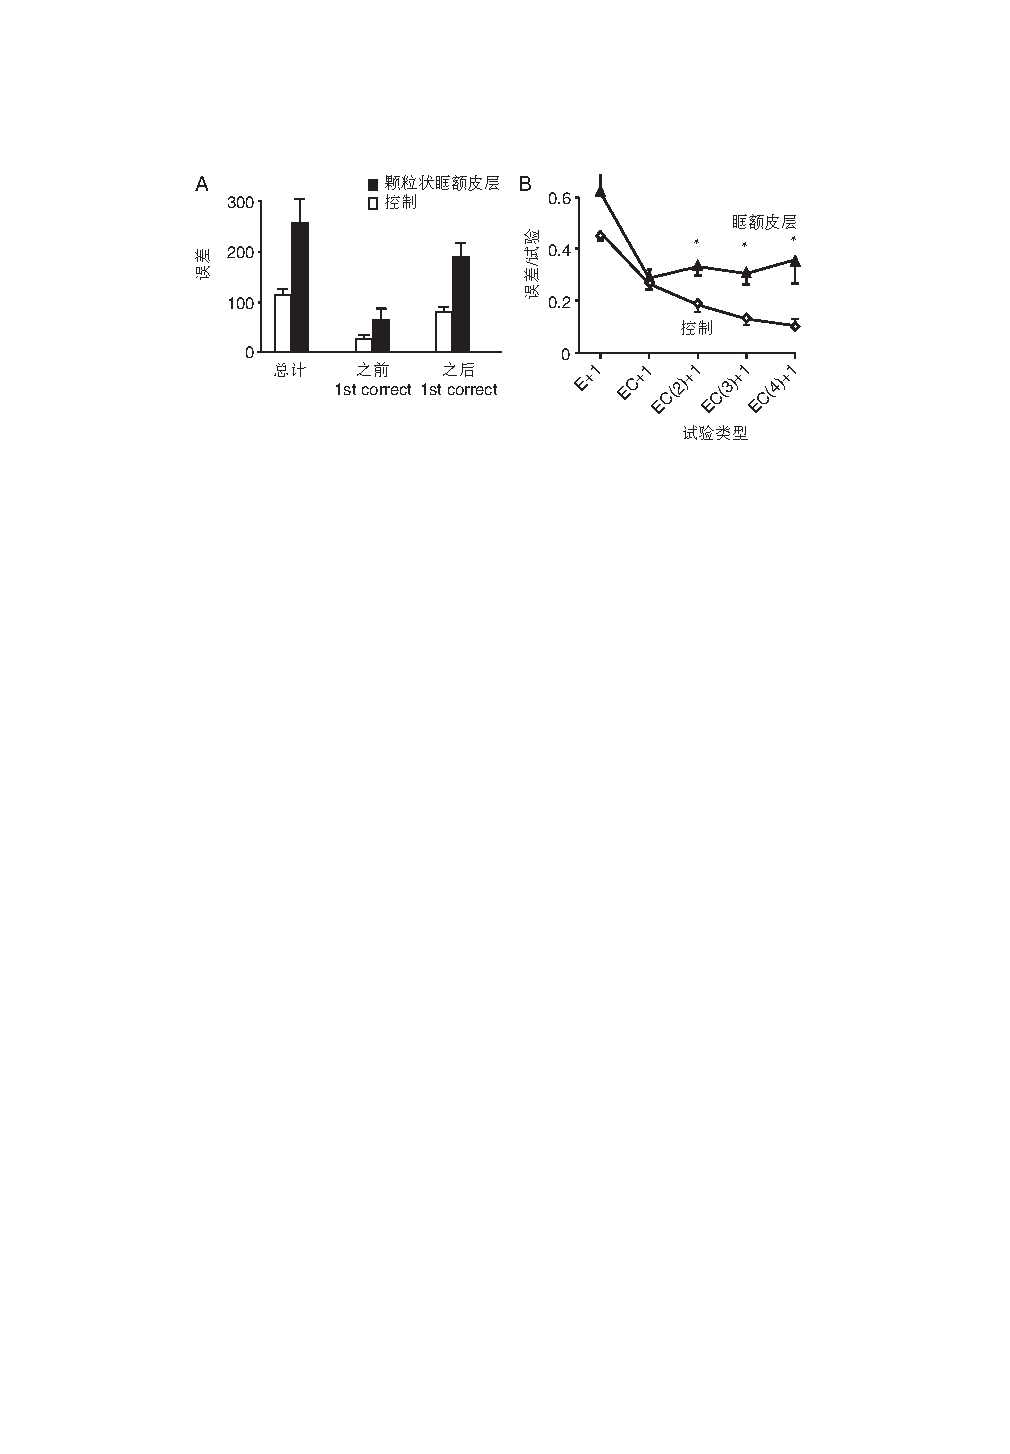
\includegraphics{chap4/fig_4_8}
	\caption{(A) 在第一次正确选择之前和之后,在对象反转任务上犯的错误。
		为了有颗粒状眶额皮层损伤的猴子(黑条)和正常(对照)猴子(白色条酒吧)。
		大多数错误出现在第一个正确选择之后。
		(B) 错误后的逐个试验性能(E + 1),在一系列错误之后是一个正确的选择 (EC + 1),在一个错误之后是两个连续的正确选择 [EC(2) + 1],等。
		粒状眶额皮层(实心三角形)无法像正常(对照)猴子(白色菱形)那样有效地受益来自奖励的积极反馈。
		星号:统计显着差异。
		误差线:SEM\cite{rudebeck2008amygdala}。}
	\label{fig:fig_4_8}
\end{figure}


\begin{figure}[!htb]
	\centering
	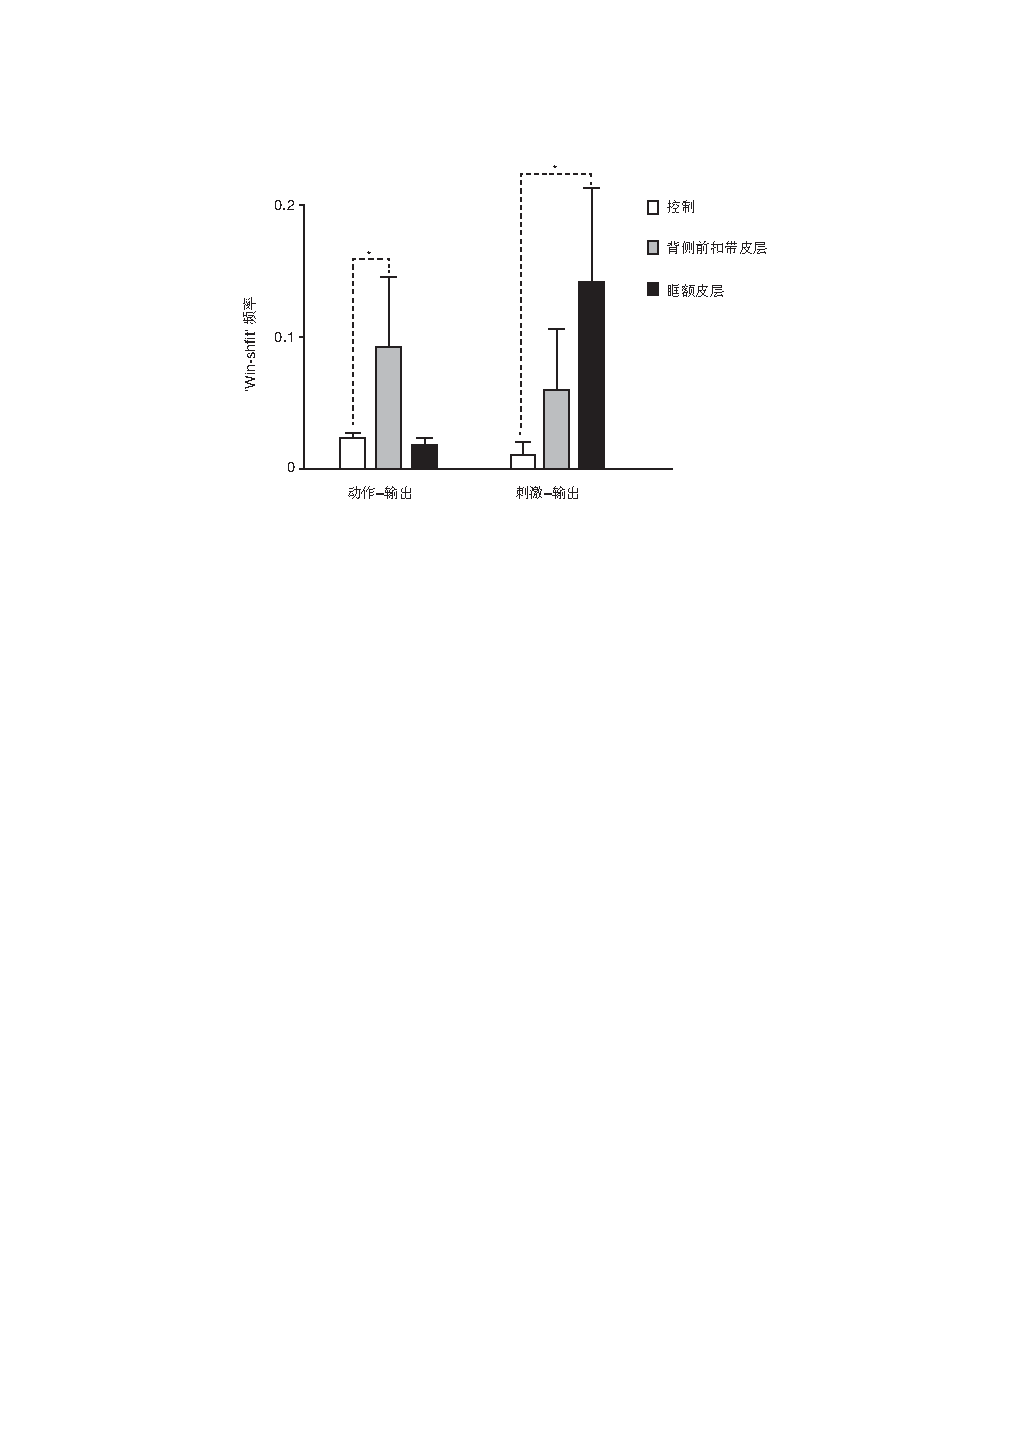
\includegraphics{chap4/fig_4_9}
	\caption{眶额皮层(黑条)和病变患者的逆转损伤与对照组(白色条)相比,前扣带皮层(灰色条)。
		为了对象反转任务,受试者在不同颜色的牌组之间进行选择;
		为了行动逆转任务,他们在旋前或旋后运动之间进行选择。
		在“胜利”之后换档,“win-shift”频率,与图~\ref{fig:fig_4_8}~中猴子所说明的错误类型相同。
		错误酒吧:SEM。
		星号:统计上显着的对比。
		转载自 Camille N, Tsuchida A,研究员LK。
		人类刺激价值和行动价值学习的双重分离眶额或前扣带皮层损伤\cite{camille2011double}。}
	\label{fig:fig_4_9}
\end{figure}


除了证明眶额皮层和内侧前额叶皮层之间的功能分离外,Rudebeck 和 Murray 在猴子身上的发现以及 Camille 等人的发现。
在人类中证明,患有眶额皮层皮层损伤的受试者使用正反馈的效率低下,但几乎可以正常使用负反馈。
这些发现直接与眶额皮层损伤的受试者由于无法抑制习得反应而坚持不懈的观点相矛盾。
事实上,这些实验中的受试者改变了他们之前的选择几乎正常,基于负面(错误)反馈。
与坚持不懈不同,这种损害可以被描述为坚持不力:与坚持不懈相反。
第~\ref{chap:chap10}~章更详细地讨论了行为抑制和坚持以及整个前额叶皮层。
在对象反转实验中,猴子会收到两种反馈,表明刺激-结果映射已发生变化:预期奖励未发生或意外奖励发生。\par
这两种情况都会导致“奖励预测错误”\cite{schultz2000neuronal}。
对中脑多巴胺能神经元的研究表明,当意外奖励到来时,活动会增加,而当预期奖励未能实现时,活动会减少\cite{schultz1998predictive}。
在第~\ref{chap:chap3}~章中,我们将此属性称为有符号误差信号,以便将其与内侧前额叶皮层中出现的无符号误差信号进行对比。
多巴胺能细胞将它们的轴突发送到纹状体和皮层,以及其他大脑结构,这些结构使用这些带符号的错误信号来调整行为。\par


奥多尔蒂等人\cite{o2003temporal}使用了一种时间差分学习模型,该模型取决于奖励预测误差。
他们在执行一项使用复杂的颜色和形状模式作为刺激的任务时扫描人类受试者。
其中一个刺激信号发出一滴甜味液体的信号,第二个刺激信号表示没有液体,第三个刺激信号发出中性味道的液体信号。
然而,在一些试验中,预测的事件没有发生。
奥多尔蒂等人寻找与签名奖励预测错误信号预期模式相匹配的激活:
当甜味未能按预期发生时激活减少,而当甜味意外发生时激活增加。
眶额皮层和纹状体腹侧部分的激活与这种模式相匹配。
当然,这些信号也可以在前额叶皮层的其他部分找到。
如第~\ref{chap:chap3}~章提到,猴子内侧前额叶皮层中的神经元也编码各种奖励预测错误\cite{matsumoto2007medial,seo2007temporal,hayden2011surprise}。
然而,对于内侧前额叶皮层,错误信号似乎主要涉及动作之间的选择,而在 O'Doherty 等人\cite{o2003temporal}的影像学研究中他们涉及刺激之间的选择。\par



\subsection{编码刺激-结果映射}

第~\ref{chap:chap3}~章解释了内侧前额叶皮层中的细胞具有反映视觉刺激价值的活动,包括成本和收益。
正如我们在那里提到的,类似的活动发生在眶额皮层中。 
肯纳利等人\cite{kennerley2009evaluating}例如,研究了奖励金额、奖励概率和多次按键的努力成本等变量。
当猴子必须在不同价值的刺激之间做出选择时\cite{seo2008cortical}以及当它们只是观察刺激和价值之间的关联时,眶额皮层中的细胞编码这些变量,就像在巴甫洛夫条件反射中发生的那样\cite{morrison2009convergence}。\par


简而言之,文献表明,眶额皮层的神经元活动不仅编码物体和奖励的价值\cite{padoa2006neurons}和获得奖励的概率\cite{kennerley2009evaluating},而且还编码影响觅食选择的许多其他因素。
这些因素包括有益和有害的结果\cite{morrison2009convergence},包括努力成本\cite{kennerley2009evaluating}、时间\cite{roesch2005neuronal}和风险\cite{o2010coding},以及 结果会出现拒绝选择\cite{abe2011distributed}和对选择成功的信心\cite{kepecs2008neural}。\par


相关的神经生理学研究强调了相对价值,这反映在对不同种类食物和液体的偏好上。
Tremblay\cite{tremblay1999relative}研究了颗粒状眶额皮层中的神经元活动。
例如,当猴子在苹果和谷物之间做出选择时,细胞可能对苹果有更大的反应,但当猴子在香蕉和苹果之间做出选择时,细胞对苹果的反应可能更小。
这些细胞编码食物的相对价值。
除了相对估值外,颗粒状眶额皮层中的一些神经元编码独立于可用选择的值\cite{padoa2009range}。
这些属性来自连接,但内侧前额叶皮层中的细胞也编码刺激预测结果的值似乎令人费解\cite{kennerley2009evaluating}。
激活也发生在内侧前额叶皮层以选择对象\cite{behrens2007learning,glascher2009determining},并且那里的损伤可能会对对象选择产生一些影响\cite{camille2011double}。
乍一看,行动-结果和刺激-结果编码之间的严格二分法似乎排除了这些结果。
如前所述,眶额皮层的损伤导致物体之间逆转的损伤\cite{rudebeck2006separate},而内侧前额叶皮层的损伤导致动作之间逆转的损伤\cite{kennerley2006optimal}。\par


基于这些结果,人们可能会假设内侧前额叶皮层应该缺乏反映刺激-结果结合的活动。
然而,第~\ref{chap:chap1}~章解释了为什么病变研究会产生与记录或成像结果似乎不一致的结果,至少在表面上。
部分原因在于眶额皮层和内侧前额叶皮层协同工作。
通过密集的互连,他们可以将刺激-结果连词与行动-结果连词结合起来。
可供性的概念有助于解释这些高阶表示。
术语可供性指的是与一个对象或一类对象相关联的动作。通过结合对象-结果和动作-结果关联,内侧前额叶皮层可能编码与以某种方式作用于对象相关的结果,在对象操作期间发生。
因此,这些表示包括对象的特征和与对象相关联的动作。
这个想法可以解释为什么对象值连接在内侧前额叶皮层中如此突出;
对象可以参与许多不同类型的动作。
这些细胞也可能编码比具体的行动-结果关联更抽象的东西,例如预测对某个对象进行任何操作或对它进行某类操作的结果。\par


如果内侧前额叶皮层的某些部分代表动作、物体和结果的结合,这可能解释了成像和细胞记录结果,以及内侧前额叶皮层损伤对物体选择的不一致影响。
例如,我们前面提到了一些未发表的证据,表明大的前扣带回损伤会损害物体反转学习\cite{murray2006prospective},尽管在类似的任务中猴子在较小的损伤后正常执行\cite{rudebeck2006separate}。\par


内侧前额叶皮层和眶额皮层功能之间的严格二分法似乎也与另一个结果不一致。
正如内侧前额叶皮层中的细胞反映刺激-结果关联\cite{kennerley2009evaluating},眶额皮层皮层中的细胞反映动作-结果关联。
Tsujimoto 等人\cite{tsujimoto2009monkey}表明,颗粒状眶额皮层中的细胞编码猴子的动作选择,但仅在反馈(奖励或无奖励)发生的时间左右。
这些发现与病变的发现并不矛盾。
Tsujimoto 等人实验中的猴子。
在每次试验期间在视频监视器上保持可见的两个可见对象(白色方块)之间进行选择。
因此,有人可能会争辩说,细胞在反馈时编码了对象之间的选择,我们稍后会再次讨论这一发现。\par


我们的核心原则之一是,眶额皮层皮层的连接解释了为什么只有它才能执行其功能。
眶额皮层而非内侧前额叶皮层接收来自颞下皮层的输入,后者代表物体的颜色、形状和视觉纹理。
眶额皮层而非内侧前额叶皮层接收来自皮层味觉、内脏和嗅觉区域的直接输入,所有这些都与特定结果相关。
因此很容易理解为什么眶额皮层代表刺激-结果的结合,以及为什么它在根据结果选择对象方面起着必要的作用。\par



\subsection{以共同货币计价}

动物必须能够比较不同资源的价值,因为觅食选择通常涉及权衡取舍。
例如,动物可能既渴又饿。
有多少特定的液体在动机上等同于一定量的食物? 一
可能是动物以“通用货币”代表一切事物的价值,以便做出这样的选择。
这个想法是,选择的不同潜在结果,例如性、温暖和食物,在一个维度中表示,以指导选择\cite{montague2002neural}。
奖励预测误差信号具有此属性。
如果神经表征中存在“通用货币”,那么无论奖励的性质如何,我们都应该看到对不同类型的同样偏好的奖励做出类似程度的反应。
Padoa-Schioppa\cite{padoa2006neurons}在编码果汁价值的猴子眶额皮层,与果汁的种类无关。
从这个意义上说,一些眶额皮层细胞编码奖励的抽象价值:以通用货币奖励。\par


对于人类主体来说,金钱作为一种奖励,它的抽象性在于它可以换取多种商品。
奥多尔蒂等人\cite{o2001abstract}教人类受试者一项针对金钱奖励的视觉辨别任务,收益与损失的激活在于头侧腹内侧 前额叶皮层,14 区。
Kim 等人\cite{kim2011overlapping}在受试者看到视觉刺激时对其进行扫描,其中一些与不同数量的金钱相关,另一些与不同数量的果汁相关。
里面有激活腹内侧前额叶皮层(14 区)与钱的数量和果汁的数量有关。\par


同样,Sescousse 等人\cite{sescousse2010architecture}将金钱的激活与色情刺激的激活进行了比较,认为后者对应于主要奖励。
他们发现了一个尾部组织,其主要奖励导致尾部和更抽象的激活,“共同货币”奖励导致吻侧激活。
其他人也提出了类似的建议\cite{kringelbach2004functional}。\par


显然,以通用货币计算估值的能力具有优势。动物经常需要平衡各种成本和收益。
并且,在某个水平,一个完全处理单一维度的觅食结果的系统可以有效地发挥作用。
用关于特定结果的高维信息增强这个系统也提供了优势,特别是对于了解对比结果之间。
稍后我们讨论证据表明眶额皮层的外侧部分以高维方式编码输出,而内侧部分以单一方式编码结果“共同货币”维度。\par


除了正面估值外,颗粒状的眶额皮层也在负面估值中发挥作用。
例如,在对蛇恐惧的研究中,猕猴伸手越过中性物体或橡皮蛇取回食物。
正常的猴子只能越过蛇经过长时间的拖延,有时甚至根本拒绝这样做。
颗粒状眶额皮层损伤后,然而,猴子很快就伸手去拿食物,拿中性物体也一样和蛇\cite{izquierdo2005comparison}。
对这一结果的一种解释是,猴子没有对蛇的负估值进行编码。
\par



\subsection{基于结果的视觉规则}

在目前给出的示例中,相关结果涉及对象的表示,无论是食物、果汁还是金钱。
但人们也可以将结果与更抽象的事物联系起来表示,例如规则的表示。
用于辨别这些映射的测试是类似的,也。
正如实验可以评估猴子之间切换的能力一样对象之间的选择,因此可以评估在规则之间切换的能力。\par


巴克利等人\cite{buckley2009dissociable}研究了学习了样本匹配任务的猴子涉及两种不同的匹配规则。
样本刺激出现后经过一段延迟后,猴子面临三种选择刺激。
潜在选择之一匹配样品的形状,另一个匹配它的颜色,第三个匹配既不是形状也不是颜色。
猴子必须使用两个匹配规则之一:匹配形状或颜色匹配。
首先,他们学习了一条规则以达到高水平的表现,然后实验者改变了这条规则。
在随后的一系列试验中猴子不得不使用新建立的规则,除了奖励或非奖励之外没有其他提示来指导它们。
这些实验类似于对象反转和动作反转前面描述的任务。\par


为了研究眶额皮层损伤的影响,Buckley 等人。
采用了与 Rudebeck\cite{rudebeck2008frontal}使用的相同的逐个试验分析,本章前面部分对此进行了解释。
该分析衡量动物坚持正确规则的可能性有多大作为最近奖励的函数。
规则更改后,Buckley 等人。
比较性能错误后进行一次试验,错误纠正序列后进行一次试验,依此类推。
前在病变处,猴子在错误纠正序列后的正确率为 77\%。
那也就是说,他们使用正确试验的积极反馈来提高他们的表现,下次他们必须在两种视觉规则之间做出选择。
眶额皮层损伤后,在错误纠正序列之后,猴子的表现只有 50\% 是正确的。
这一发现表明眶额皮层在将结果与选择相关联方面起着重要作用,规则之间以及对象之间的选择。\par



\subsection{更新激励估值}

特定食物奖励的当前价值也反映了当前的生物需求或动物的状态。
第~\ref{chap:chap3}~章解释了贬值任务操纵食物的价值,有时是通过选择性的饱食程序:猴子消耗一种食物测试前的饱腹感。\par


伊兹奎尔多等人\cite{izquierdo2004bilateral}教猴子选择一组对象产生一种食物,而对另一组对象的选择产生了另一种食物。在所有训练课程中,与两种食物之一相关的物体(正对象)与一个对象配对,如果选择该对象,则不会导致奖励(中性对象)。
这猴子很好地学习了这些对象-结果映射。
然后猴子吃掉其中一种食物直到饱足,这个过程会降低食物的价值。
然后,在随后的测试阶段,当猴子吃饱的时候,他们面临两个选择:正物,每一种食物一个。
没有任何选择的经验,这两个积极的对象,正常的猴子仍然倾向于避免选择对象与贬值的食物有关。
相反,他们选择了与最适合他们当前动机状态的结果:价值更高的食物。
他们每对物体只看到一次,因此不能根据测试期间的经验做出选择。
因此猴子们一定做出了他们的选择基于对结果的预测,并更新该结果的值,他们当前的动机状态。\par


相比之下,具有颗粒状眶额皮层损伤的猴子并没有避免贬值的选择几乎和正常猴子一样有效(图~\ref{fig:fig_4_10})。
相反,他们倾向于根据他们最初的食物偏好选择对象。
因此,如果一只受伤的猴子最初偏爱一种食物,它们就会倾向于选择与该食物相关的物品食物,即使他们刚刚吃饱了。\par


\begin{figure}[!htb]
	\centering
	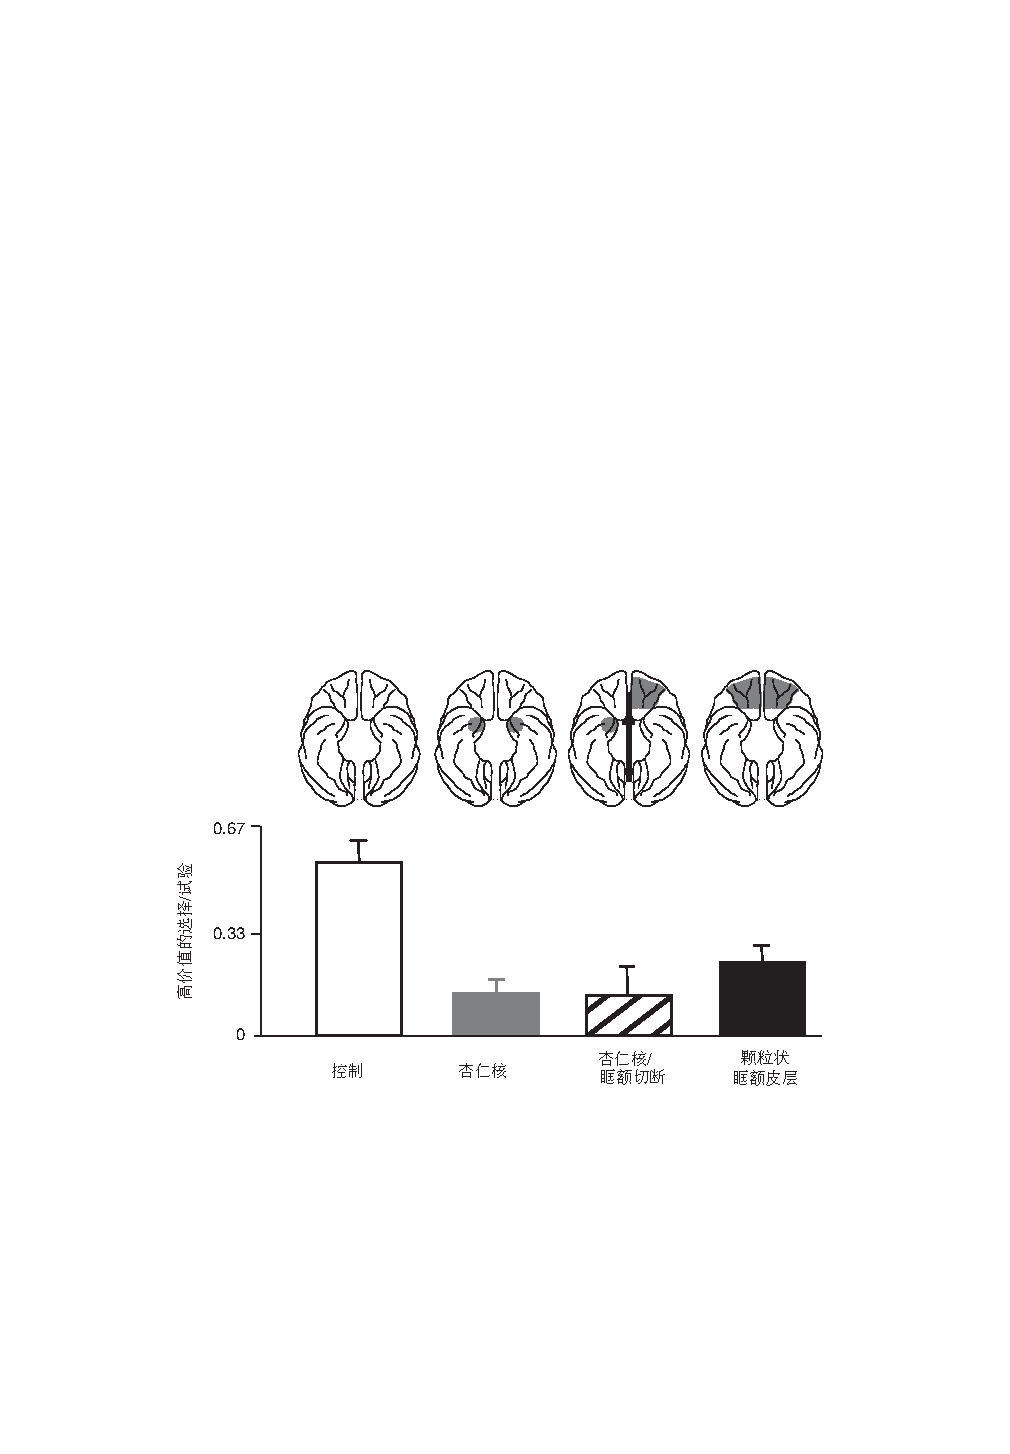
\includegraphics{chap4/fig_4_10}
	\caption{不同病变对选择贬值任务表现的影响。
		上图描绘了猕猴大脑腹侧视图中的三个损伤。
		阴影表示选择性杏仁核病变的大致位置(在大脑表面下方)或颗粒状\textit{眶额皮层}。
		大脑半球之间的粗黑线表示胼胝体和前连合的横断。
		顺序:每次试验中高价值选择的比例,也就是说,选择的对象没有因先前的选择性饱腹而贬值。
		误差条:SEM\cite{murray2007orbitofrontal}。}
	\label{fig:fig_4_10}
\end{figure}


如图~\ref{fig:fig_4_10}~所示,杏仁核的双侧损伤会产生类似的效果,并且它还伴随着杏仁核的单侧损伤和颗粒状损伤大脑另一侧的眶额皮层\cite{baxter2000control}。
腹侧病变前额叶皮层或中外侧前额叶皮层没有这种效果\cite{baxter2009ventrolateral}。\par


其他证据表明,当猴子吃饱时,动机评估的更新会自动发生。
期间杏仁核失活进食会导致损伤,但后来的失活不会(Wellman 等人,2005 年)。
这发现表明杏仁核和眶额皮层之间的相互作用必须发生在进食期间,因为食物的价值因饱食而改变。\par


眶额皮层的连接解释了为什么它在此功能中起着至关重要的作用。
为了做出最佳的觅食选择,猴子必须根据当前的情况做出选择动机评价,这需要它与杏仁核的联系。
猴子颗粒状眶额皮层或杏仁核的损伤仍然饥饿,因此有动力觅食,但他们不再根据当前的需要做出选择。\par


对猴子进行的损伤实验表明,颗粒状眶额皮层会影响估值更新。
人们的成像结果指向相同的结论。
戈特弗里德等人\cite{gottfried2003encoding}教人类受试者将一种视觉刺激与某种气味联系起来,并将不同的视觉刺激与另一种气味联系起来。
然后受试者吃饱了具有一种或另一种气味的食物,后来在偏好中表现出贬值效应测试,很像猴子。
杏仁核和眶额皮层激活的变化皮层平行于偏好的变化。
峰值激活坐标出现在颗粒状眶额皮层。
当然,这一发现并不排除颗粒状眶额皮层在
其他类型的估值更新。\par


同样,Critchley\cite{critchley1996hunger}从颗粒状眶额皮层中的细胞记录,同时猴子闻到气味或看到与特定果汁相关的视觉刺激,比如黑莓汁。
在猴子饮用一种果汁达到饱足感后,细胞降低了他们对与之相关的嗅觉或视觉刺激的反应,一种果汁。\par


将我们在这里所说的内容与第~\ref{chap:chap3}~章放在一起,我们可以看到内侧前额叶皮层和眶额皮层都发生了动机评估的更新,对于这两个动作——结果和刺激-结果连词,对于“内部”引导和外部引导的选择,以及颗粒状和颗粒状前额叶皮层。
一些组合还有待测试,例如颗粒状眶额皮层的特定贡献在猴子中。
但是我们假设价值更新是通过杏仁核及其所有皮层区域。
我们并不是要暗示这一种更新涵盖了杏仁核的所有功能,但它似乎是一种重要的一个。\par



\subsection{信用分配}

在前面描述的对象反转实验中,结果取决于猴子在两个对象之间的选择。
觅食的一个重要方面涉及学习什么选择会导致行为结果,而这种知识很少是确定的。
沃尔顿等人\cite{walton2010separable}因此设计了一个实验来探索眶额皮层如何分配特定结果对刺激物中特定选择的因果责任。\par


在三臂强盗任务(图~\ref{fig:fig_4_5}B)的每次试验中,猴子看到三种刺激,其中包含多种形状和颜色。
如果选择,每种刺激产生奖励的概率都不同。
这些概率随时间而变化,无论是在高波动率和低波动率模式。
图~\ref{fig:fig_4_6}~显示了奖励概率,三个刺激作为时间的函数。
面对这个问题,猴子通常会选择产生最大收益的刺激。
在图示的实验中在图~\ref{fig:fig_4_6}~中,经过大约 145 次试验后,之前完全没有效果的刺激开始这样做了。
经过多次试验,它还清的可能性超过了其他两种可能的选择。
正常的猴子需要一些时间才能发现这个事实,但之后
大约 150 次试验,他们始终选择这种新的最佳刺激。
值得强调的是,与一些类似的实验不同,在这个实验中,猴子之前的选择并没有影响支付概率:结果根据预先确定的时间表变化。\par


具有颗粒状眶额皮层损伤的猴子需要更长的时间才能发现新的在其收益概率超过竞争刺激后的最高价值刺激。
图~\ref{fig:fig_4_6}~表明,经过大约 10 次试验后,正常猴子和眶额皮层皮层损伤的猴子出现分歧,此后受损的猴子做出了明显次优的选择,这种选择持续了 150 多次试验,只有一点改进。\par


原则上,减值可能反映了行为灵活性的丧失,但高波动性条件排除了这种解释。
如图~\ref{fig:fig_4_6}~所示,当其中两个概率显着波动正常和受损的猴子灵活变化,他们的选择,尽管程度不尽相同。
如果猴子缺乏灵活性或都在坚持,他们本该坚持同样的选择。\par


沃尔顿等人然后取得了关键性的突破。
在以前的低价值刺激超过其他刺激后,他们仔细分析了试验结果。
在那一刻,它成为了“最近最好的”刺激,与“以前最好的”刺激形成对比。
如果,在它大涨之后在价值上,猴子选择了这个“最新最佳”刺激并获得了奖励,它应该更有可能在下一次试验中再次选择相同的刺激。
正常的猴子会正是这样,但具有颗粒状眶额皮层病变的猴子却没有。\par


图~\ref{fig:fig_4_11}~显示了猴子做了什么以及为什么。
y 轴上的正值表示猴子增加他们对“以前最好的”刺激的选择的程度。
负值表示他们将选择转向“最新最佳”刺激的程度。
该图说明了关键发现。
对于正常的猴子,获得选择奖励“最新最佳”刺激措施导致他们的选择转向该刺激措施。
对于有损伤的猴子,情况正好相反。而且选择“以前”的历史越长最好的”而不是“最近最好的”刺激,他们选择错误刺激的次数越多。\par


\begin{figure}[!htb]
	\centering
	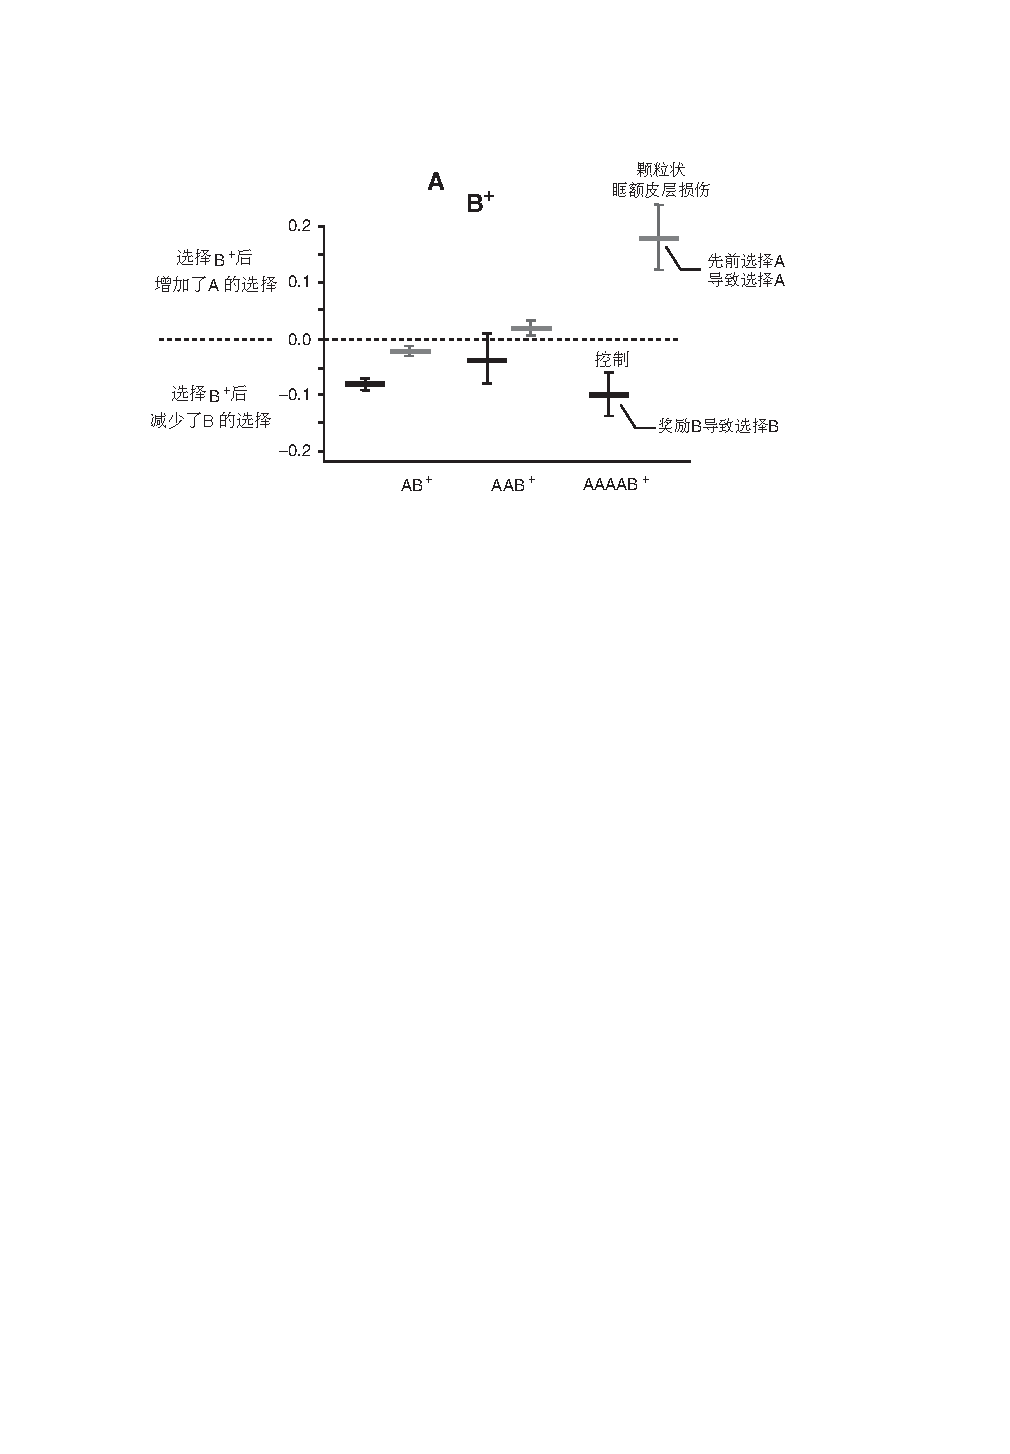
\includegraphics{chap4/fig_4_11}
	\caption{基于单个事件的信用分配。该图显示了正常(对照)猴子(黑色)和有颗粒状眶额皮层病变的猴子(灰色)的平均值(水平线)和SEM。
		横坐标根据在选择刺激B导致奖励(+)的试验之前有多少次刺激A的试验来划分试验。
		顺序:正值表示在因选择刺激B而获得奖励后选择刺激A的可能性增加;
		负值表示在该情况下选择刺激B的可能性增加\cite{walton2010separable}。}
	\label{fig:fig_4_11}
\end{figure}


这些结果表明,正常的猴子认识到它们之间的因果关系。
选择“最近最好的”刺激和结果,但受损的猴子这样做了更不准确。
相反,受损的猴子根据选择“以前最好的”刺激的历史更长。
他们似乎错误地将他们因选择“最新最佳”刺激而获得的奖励分配给他们先前选择“先前最佳”刺激的某个平均值,并赋予更多权重最近的选择。\par


图~\ref{fig:fig_4_12}~以矩阵形式以图形方式解释了该结论的基础。
图显示结果和试验中选择的对象之间映射的强度。
“适当的”分配会将 $ n $ 次试验中发生的结果从当前试验映射回猴子在该试验中做出的选择。
也就是说,他们应该归因于上次试验的结果与他们在那次试验中的选择(一回)有关,他们应该
将前三次试验的结果归因于他们在前三次试验中做出的选择(三回)。
正常的猴子为“正确的”建立强关联映射任务,在这个意义上。
只有弱映射(如果有的话)才会从结果到“不正确”的选择。
该图显示了一些示例,例如结果之间的弱映射三试回与选择作出一试回。
有颗粒状病变的猴子眶额皮层无法像正常猴子那样有效地建立强大的、“适当的”映射。\par


\begin{figure}[!htb]
	\centering
	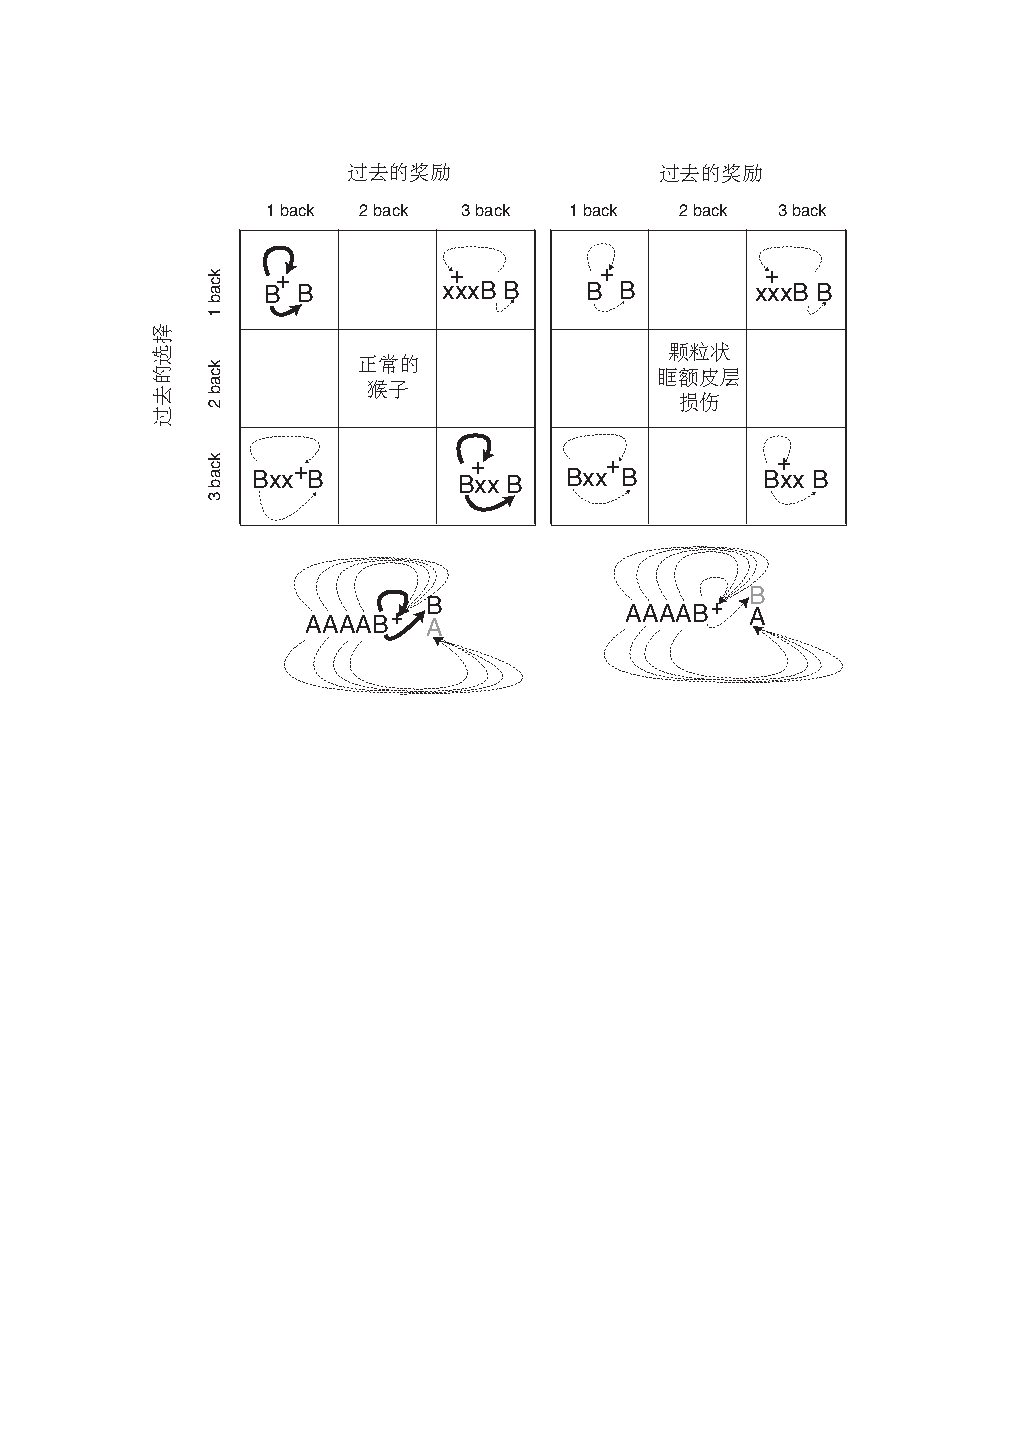
\includegraphics{chap4/fig_4_12}
	\caption{每个矩阵显示选择和奖励之间的选定映射。
		猴子在A、B和C三种刺激中进行选择。B是奖励选择,如加号(+)所示。
		x表示可供选择的选项(A或C)。
		左图:正常(对照)猴子的信用分配,基于单个事件。
		例如,在矩阵的左上角和右下角细胞中,刺激B的选择被分配给适当试验的结果(+),这促进了未来B的选择。
		或者,可以说结果被分配给了选择。
		实线表示强烈的影响;虚线表示弱的。
		右图:在患有颗粒\textit{眶额皮层}病变的猴子中,对结果进行单一选择的障碍。
		只剩下微弱的影响。在每个矩阵下面是对这种机制的概括描述。
		黑色表示所选择的刺激;灰色,未选择的刺激。
		强影响反映了单一选择-结果事件(实线),弱影响反映了许多结果事件的时间加权平均值,如不同深浅的灰色(虚线)所示。
		由于失去了单一反馈事件的强大影响,受损猴子更经常选择刺激a(右),而在正确的信用分配的基础上,正常猴子更经常地选择刺激B(左),如图~\ref{fig:fig_4_11}~所示。}
	\label{fig:fig_4_12}
\end{figure}


沃尔顿等人的发现。
因此可以理解为表明颗粒状眶额皮层改善“信用分配”,定义为将结果分配给选择似乎是造成它的原因。
人们可以将此重述为将选择分配给结果似乎导致:选择-结果映射。
因此,粒状眶额皮层的功能似乎涉及使用单一结果事件进行分配的重大改进单项选择事件的因果责任。\par


至关重要的是,患有颗粒状眶额皮层病变的猴子表现得像老鼠。
像老鼠一样,这些猴子有一个颗粒状的眶额皮层,像老鼠一样,它们的选择基于通过将选择和结果的整体历史与有时称为改善的新近度偏差联系起来的选择-结果映射的近似值\cite{herrnstein1991melioration}。
改善是指增加反应的过程,最近有效,随时间平均,不参考具体事件。
所以像老鼠一样,由于不同的原因缺乏颗粒状眶额皮层,颗粒状损伤的猴子眶额皮层不再根据选择事件的“适当”分配做出觅食选择结果事件,而不是使它们基于更广泛的平均数,偏向于最近成功的选择。\par


Tsujimoto 等人\cite{tsujimoto2009monkey}展示了信用分配如何在单细胞中起作用,前面提到的神经生理学实验中的水平。
他们研究了线索策略任务中的神经元活动。
视觉提示指示猴子留在原地或移动来自他们之前在两个空间目标之间的选择。
他们发现神经元在当结果发生时,颗粒状眶额皮层编码了猴子对空间目标的选择。
围绕结果时间的选择表示可以促进准确学分分配。\par


Tsujimoto 等人还比较了这些选择在正确和不正确执行的试验中的编码,正如第~\ref{chap:chap3}~章提到的额极皮层一样。
他们假设在正确的试验中,猴子的选择基于特定的认知过程:一个提示停留转移策略。
猴子们很好地完成了任务,所以“幸运”的猜测可以对结果贡献不大。
猴子确实犯了一些错误,这可能是在他们忘记了一些对他们来说很重要的事情之后,他们随机选择了一个目标
任务。
不同于前额叶皮层其他部分的细胞,例如额极皮层和中侧 前额叶皮层,眶额皮层眼眶中的细胞在正确和错误试验中具有相同的活动(图~\ref{fig:fig_4_13})。
这一发现表明,无论产生它们的认知过程,至少在具有固定奖励概率的任务上并且不需要学习\cite{tsujimoto2011frontal}。
在这种情况下,如果眶额皮层将信用分配给特定的选择,无论如何,它似乎都会这样做,猴子做出了那个选择。\par


\begin{figure}[!htb]
	\centering
	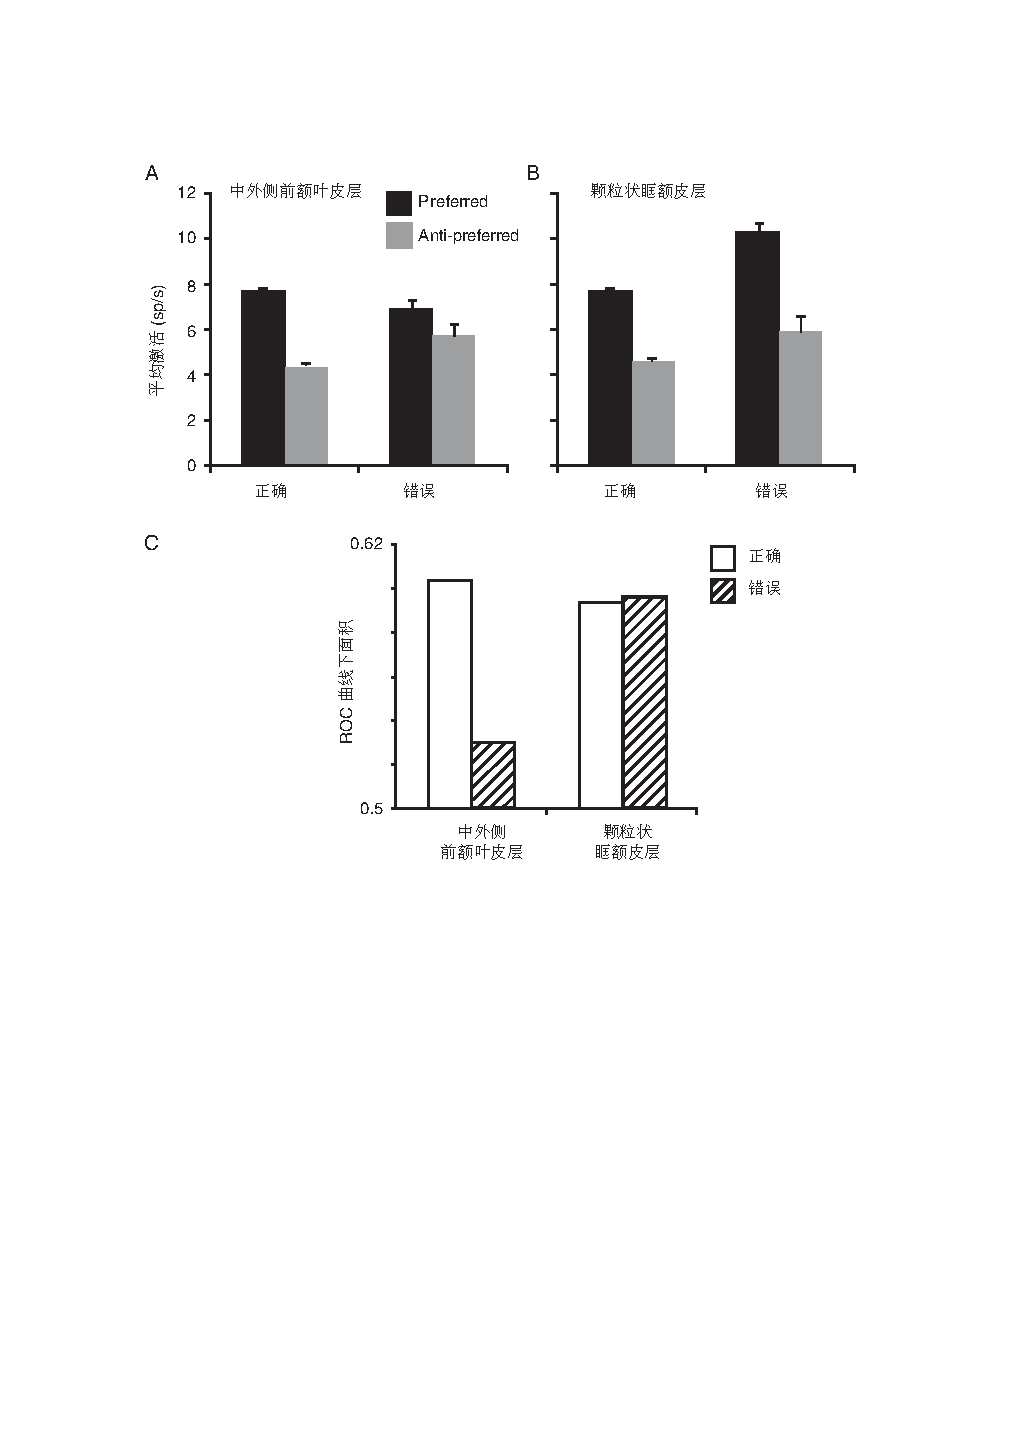
\includegraphics{chap4/fig_4_13}
	\caption{猴子在反馈期的细胞活动编码选择。
		(A) 对于中外侧前额叶皮层,在正确执行的试验中,首选(黑色)选择的平均群体活动显著超过反首选(灰色)选择的群体活动,但在错误执行的试验(错误)中没有。
		(B) 相比之下,颗粒状\textit{眶额皮层}中的细胞在正确和错误试验中都对选择进行了显著编码。
		(C) 同样的结论来自于对细胞活性的接收操作特征(ROC)的分析,该分析测量了理想观察者根据细胞活性水平在每次试验中检测选择的能力。
		请注意,在中外侧前额叶皮层的错误试验中,ROC值降至0.53,这对应于机会水平。
		缩写:sp/s,每秒峰值\cite{tsujimoto2011comparison}。}
	\label{fig:fig_4_13}
\end{figure}



\subsection{颗粒状眶额皮层的细分}

到本节的这一点为止,我们已经从整体上讨论了粒度 眶额皮层。
然而在在本章的开头,我们引用了不同的解剖学权威来划分这个区域分为至少三个皮层区域:区域 11、13 和 14。
基于连接,Carmichael 和 Price 将区域 14 放置在一组他们称为中间网络的区域中,他们将其归因于内脏运动功能。
相比之下,11 区和 13 区的大部分地区属于眼眶网络,与皮层的感觉区域有很强的联系,比如下颞皮层。\par


最近的实验探索了大脑内侧部分的功能特化颗粒状眶额皮层,与横向部分相反。
其中一组研究的重点是关联映射,另一个关于动机估值。
为了方便,我们使用术语外侧和内侧眶额皮层,但读者应该记住我们指的是在所有情况下到细粒度的眶额皮层。\par


努南等人\cite{noonan2010separate}特别比较了内侧和外侧眶额皮层部分的作用,使用前面解释的三臂老虎机任务(图~\ref{fig:fig_4_5}B~)。
涉及 14 区颗粒状部分的内侧损伤并未损害猴子的能力将功劳分配给选择。
外侧眶额皮层的损伤导致了这种损伤。
14 区的损伤造成了不同的损伤。
有这些损伤的猴子当“最近最好的”和“以前最好的”刺激的价值相差很小的概率时,就会出现次优选择。
与“最新最佳”相关的第三种刺激的价值刺激也影响了他们的选择。努南等人得出结论,内侧眶额皮层有助于比较不同结果的价值,在它们被分配后到特定的选择刺激。
他们建议,它是根据“共同货币”来实现的,即如前所述,价值的一维表示。\par


神经影像学研究支持这些想法。
O'Doherty\cite{o2001abstract} 之前审查的研究等和Kim 等人\cite{kim2011overlapping}指出与多种结果相关的区域 14的激活,正如预期的“共同货币”价值表示一样。\par


在另一项影像学研究中,Noonan 等人\cite{noonan2011distinct}让人们在对象之间进行选择。
结果包括受试者可以使用的视觉呈现的礼券之后。
一种证书可以用来购买音乐和视频,另一种证书,咖啡馆的第三种食物,等等。
在一种情况下,给定的选择总是导致一种特殊的礼券; 在另一种情况下,给定的选择产生随机结果。
因此,受试者学习了他们的选择和选择之间的关联映射。
前一种情况下的特定类型结果,而后一种情况下则不然。\par


努南等人当人们将功劳归功于特定选择的结果,而他们在内侧眶额皮层中发现激活人们使用结果值来指导选择。
具体来说,他们发现更大当给定的之间存在一致的关系时,外侧眶额皮层的激活选择和一种结果。
在这种情况下,横向眶额皮层增加了耦合具有代表物体的区域,例如鼻周皮层,以及有助于更新动机评估的大脑结构,例如杏仁核。\par


相比之下,Noonan 等人在内侧眶额皮层中发现了不同的激活模式。
那里的激活并没有反映出结果是否让人们了解了特定的选择-结果映射。
相反,它与预测结果的价值成正比。
这一发现与 Noonan 等人的发现一致\cite{noonan2010separate}。
在猴子中获得内侧眶额皮层病变。\par


这些发现与神经生理学研究的结果大致相符。
在横向眶额皮层,细胞编码指示结果价值的视觉刺激,而不是口渴程度本身\cite{bouret2010ventromedial}。
虽然有些细胞位于外侧眶额皮层随着猴子对奖励感到满意,活动减少,与根据\cite{critchley1996hunger}的结果,这种性质在眶额皮层内侧部分的细胞\cite{bouret2010ventromedial}。
这一发现与区域 14 在比较“通用货币”的结果值中的作用一致基于当前的动机状态。\par


布罗德森等人\cite{brodersenorbitofrontal}在影像学研究中区分相同区域哪些受试者执行了三臂强盗任务(图~\ref{fig:fig_4_5}B)。
主题选择刺激,产生概率结果。
这些结果提供了反馈关于三种情况下的每个选择:在同一次试验中,延迟一次试验,或延迟,通过随机数的试验。
在前两种情况中的任何一种情况下,受试者都可以将结果分配给以前的选择,但在第三个选择中他们不能。\par


布罗德森等人在前两个条件中的任何一个中发现在横向 眶额皮层中的激活比在第三个随机条件中更多。
他们得出的结论是,激活反映了他们的受试者是否可以在结果和特定选择之间分配因果责任。
他们的结果也排除了他们的激活反应的可能性结果以任何简单的方式或它反映了奖励预测错误。\par


这些更精细的细分在贬值和灭绝实验中有相似之处前面讨论过。
回想一下,颗粒状眶额皮层的损伤会导致贬值任务。
有缺陷的猴子不会根据当前的需要做出选择。
具有相同病变的猴子也表现出比正常人更慢的“灭绝”学习。
Rudebeck\cite{rudebeck2011dissociable}对外侧眶额皮层进行了选择性损伤(对应于11 区和 13 区的部分区域),发现它们对贬值任务。
一项独立研究获得了类似的结果\cite{machado2007effects}。\par


内侧眶额皮层的病变,包括 14 区,不影响对贬值的选择任务。
相反,它们对消退任务造成了轻微的损害,这些损害外侧 眶额皮层不受影响。
同样的损害也影响了基于价值的传递性测试的选择。
在这个测试中,猴子在与之相关联的对象之间进行选择不同的熟悉的食物,其中他们有排名的偏好。
猴子与正常猴子相比,内侧眶额皮层病变(区域 14)做出更多违反其整体食物偏好的选择,但具有外侧眶额皮层病变(区域 11 和 13)的猴子没有表现出这种效果\cite{rudebeck2011dissociable}。\par


有两种方法可以查看与货币贬值相关的贬值任务的结果选择-结果协会的学习。
一种观点认为,横向眶额皮层执行两个相关功能。
它学习选择-结果映射,并更新基于当前生物学需求的结果的动机评估。\par


或者,损害可能完全是由于难以学习关联映射。
按照这种观点,无法将不同的结果分配给对象正确的选择可能会导致贬值任务的赤字,尤其是当猴子需要学习选择和结果之间的许多关联。
也许有外侧眶额皮层损伤的猴子可以了解到一个物体与奖赏有关一般意义上的,但是因为他们学习对象和对象之间的关联的速度很慢特定奖励的感官特性,他们不知道哪种奖励可能。\par


与后一种解释相反的事实是,在贬值任务中,猴子不会需要学习物体和食物之间的新关联:他们似乎已经学会了这些关键测试会话之前的映射。
然而,它们仍然显示出贬值效应。
虽然这一发现并不能完全决定问题,我们赞成病变影响的观点关于贬值任务和信用分配任务反映了两个方面的选择——结果关系。
一方面涉及学习是什么选择导致了给定的结果,另一个涉及在选择时知道该结果的价值。\par



\subsection{概括}

为了总结我们对颗粒状眶额皮层的看法,我们回顾了它发挥作用的证据在对象和其他刺激之间的偏向选择中的特殊作用。
它通过使用过去的经验来预测可能遵循给定选择的结果,如更新就目前的生物学需求而言。
它还根据对象评估规则,例如按颜色或形状匹配。
所有这一切都部分取决于外部感官信号,以及他们与反映当前需求的“内部”激励信号的相互作用。\par


眶额皮层的功能补充了内侧前额叶皮层的功能,后者对行动和行动规则的选择产生偏见(第 \ref{chap:chap3} 章)。
这些选择取决于主要基于“内部”信号,例如那些代表行动、对先前事件的记忆和当前需求的信号。
然而,这并不意味着内侧前额叶没有对象估值的表示。
确实如此。 我们审查成像证据和细胞记录,表明内侧前额叶皮层在相关动作中的作用对象。\par


一组关键的调查结果表明,颗粒状眶额皮层在改善信用方面发挥着关键作用任务。
在执行此功能时,它学习、表示和更新因果关系特定对象的选择与由特定对象引起的特定结果之间的关系该选择,它可以在单个事件的基础上这样做。\par


最后,颗粒状眶额皮层的不同部分具有可分离的功能。
内侧部分根据称为价值的抽象的一维表示来评估结果一种“共同货币”。
相比之下,横向部分代表了他们许多方面的结果基于广泛特征连接的维度(图~\ref{fig:fig_4_3})。\par



\section{结论}

\subsection{眶额皮层如何发挥作用}

眶额皮层的连接解释了它如何执行其功能。
首先,它从几种感觉方式接收感觉信息。
结果,眶额皮层可以表示特征的连词,例如食物的外观和味道(图~\ref{fig:fig_4_3})。
其次,眶额皮层与杏仁核有联系,杏仁核根据当前的生物学需求更新选择的动机评估。
通过与感觉皮层和杏仁核的相互作用,眶额皮层了解对象之间的选择以及这些选择所带来的结果。
我们可以将这些和一些额外的要点总结如下:\par


1. 颗粒状眶额皮层与嗅觉、味觉和内脏皮层有关,例如,这使他们能够代表特定的感官结果——特定的气味和味道。\par


2. 眶额皮层与内侧前额叶皮层有广泛的相互联系。
这内侧前额叶皮层会在动作和动作规则之间做出选择(第~\ref{chap:chap3}~章),眶额皮层改进了关于刺激和规则的选择刺激,例如匹配颜色或形状。
因此,我们将内侧区域与“内部”引导的行为和直接的行动选择联系起来,而不是选择要采取行动的对象。
同样,我们将轨道区域与外部引导的行为和对象之间的选择联系起来。
觅食选择涉及两者,这个事实解释了为什么内侧前额叶皮层和眶额皮层必须相互作用。\par


3. 眶额皮层与基底外侧杏仁核有广泛的相互联系,这是根据当前生物学需求更新结果评估的基础。
来自猴子的证据表明,颗粒状眶额皮层的外侧部分有助于这种更新功能。
因此,特定食物或液体的价值取决于动物最近消耗了多少。
颗粒状眶额皮层也与杏仁核有关,所以我们假设类似的更新功能适用于啮齿动物和灵长类动物,也适用于颗粒状和非颗粒状眶额皮层。
然而,这个话题还需要更多的研究。\par


4. 颗粒状眶额皮层与下颞皮层和鼻周有很强的联系皮层,它提供有关物体的信息,包括它们的颜色、视觉纹理、光泽度、半透明度和形状。
他们还接收体感输入,特别是从嘴巴和舌头的表现。
结合第 1 点,这些联系允许灵长类动物构建特定食物和比它们的流体具有更高的维度和更高的特异性祖先。
这些进步反映了灵长类动物的视觉特化(第~\ref{chap:chap2} 章)。\par


总而言之,这些联系解释了灵长类眶额皮层并解释其在改善信用分配中的关键作用的能力使用单个事件为结果分配选择在很大程度上取决于灵长类动物视觉系统提供的丰富的高维表征。



\subsection{提议}

在关于内侧前额叶皮层的第~\ref{chap:chap3}~章中,我们开始制定一个最终以第~\ref{chap:chap8}~章。
在这里,我们对眶额皮层进行了简要和扩展形式的分析。\par


简单来说:
眶额皮层有助于评估和选择感官刺激基于与结果的关联,与当前需求相关。\par


展开:\par
眶额皮层通过偏向感觉刺激和基于刺激的规则之间的选择,作为一个整体促进前额叶皮层的功能。
它通过一个根据当前需求评估具体的预期结果。
在灵长类动物,它可以学习刺激中的哪种选择导致了基于特定结果的在一个事件上。
它既可以比较以共同货币计算的结果,也可以对比彼此的特定结果。\par



\subsection{为什么其他区域不能做眶额皮层所做的事情}

我们还需要解释为什么只有眶额皮层可以做它所做的事情。 
其他皮层区域也有一定程度的两种感觉方式的汇聚,有时更多,因此被称为多峰或多峰。
上颞区如\textit{上颞多感觉区}(也称为区域TPO)属于此类\cite{seltzer1994parietal},以及位于主要视觉、听觉和体感区域之间边界的其他区域,例如后部的 VIP 区域顶叶皮层\cite{schlack2005multisensory}。\par


但这些区域都没有眶额皮层具有的特征结合和模态收敛程度,尤其是在灵长类动物中。
这意味着他们不能构建图~\ref{fig:fig_4_3}~所示的连词。
同时,诸如此类的领域由于后顶叶皮层缺乏与眶额皮层所具有的杏仁核的联系,因此他们不能很容易地将他们处理的视觉信息与基于当前生物学需求的价值。\par



\subsection{对觅食选择的贡献}

眶额皮层中感觉方式的大规模汇聚允许哺乳动物链接对刺激的特定结果表示,以提高它们的觅食效率。
因此,哺乳动物可以根据食物之间更复杂的区别做出选择
或液体比他们的非哺乳动物祖先和灵长类动物可以这样做与他们的非灵长类动物祖先和大多数人相比,有更复杂的区别其他现代哺乳动物。\par


尽管在结果之间做出更精细的感官区分的能力很重要,我们认为信用分配的概念最能解释前额叶皮层功能。
动物根据预测结果做出觅食选择的事实使得将过去的结果准确地分配给产生这些结果的选择是有利的。
当然,所有觅食动物都面临这个问题,但第~\ref{chap:chap2}~章解释说,早期的灵长类动物适应了细枝生境,它们在昏暗的光线下和杂乱的树丛中觅食。
潜在的食品和非食品。
颗粒状眶额皮层在这些动物中进化,因为它们适应了这个利基市场。
本章回顾了这些领域提供当前每个对象根据动物当前需求的价值。\par


我们提出,与它们的祖先状况相比,这些早期灵长类动物可能根据单个事件改进信用分配,并且新进化的,精细 眶额皮层实现了这一进步。
具有颗粒状眶额皮层损伤的现代猴子就像老鼠和其他哺乳动物一样,它们仍然可以通过整合过去许多试验的信息来学习,但它们不能将结果归因于单一事件。
我们将这一发现用于对理解前额叶皮层的功能至关重要,我们将返回第~\ref{chap:chap8}~章中,我们将从单个事件中学习的能力与较慢的、累积的能力进行对比学习最终优化觅食选择,但需要更长的时间才能做到这一点。
没有颗粒状眶额皮层提供的因果分析的改进,猴子恢复到其他哺乳动物所具有的能力的近似值。
第~\ref{chap:chap8}~章发展这个想法在前额叶皮层功能的上下文中,作为一个整体考虑。\par


本章还回顾了证据,证明颗粒状眶额皮层的不同细分对灵长类动物在物体中做出的选择有不同的贡献。
的侧面部分颗粒状眶额皮层帮助灵长类动物回答两个关键问题:
特定食物或液体有什么作用给定的选择产生?
以及根据当前需求评估的结果是什么值得?
颗粒状眶额皮层的中间部分帮助他们回答了第三个问题:
当转化为价值的一维表示时,一种“通用货币”,如何这个选择与其他选择相比?\par


我们可以用两种方式中的任何一种来总结这种解剖学上的区别。 
一、侧面眶额皮层了解物体和其他刺激的价值,而内侧 眶额皮层通过比较这些值来调节选择\cite{noonan2010separate}; 
二、横向眶额皮层学习选择-结果映射取决于不同结果之间的对比,而内侧眶额皮层学习依赖于比较的选择-结果映射不同的结果\cite{rudebeck2011dissociable}。\par


在物体中做出选择后,灵长类动物仍然必须找到那个物体并保持在杂乱的环境中注意它。
下一章解释如何连接尾部前额叶皮层支持其在这些搜索和注意力功能中的作用。\par




\chapter{尾侧前额叶皮层:搜索目标} \label{chap:chap5}

尾侧前额叶皮层有助于通过显性注意力(眼球运动)和隐性注意力对食物和食物迹象等物体进行视觉搜索,它的连接解释了它如何执行这些功能。
尾侧前额叶皮层,包括额叶视区,与视觉皮层的背侧流和腹侧流以及脑干动眼神经核都有联系。
明显的注意依赖于它与脑干动眼核的连接,直接或间接地通过上丘和基底神经节。
隐蔽注意力依赖于增强的感觉反应,这种反应是通过与视觉皮层以及其他感觉区域的相互作用来调节的。
在早期灵长类动物中,随着眶额皮层的颗粒状部分,尾侧前额叶皮层也在进化(第~\ref{chap:chap2}~章)。
这两个新区域一起导致了在精细分支生态位的杂乱环境中发现、关注和评估物体的改进。



\section{介绍}

在前一章中,我们认为眶额皮层根据当前的生物需求对物体赋值。
本章提出,尾侧前额叶皮层搜索这些物体,它是通过隐蔽地注意周围目标和将眼睛朝向这些目标来实现的。


本章的大部分内容都是关于视觉和眼球运动的,它们在脊椎动物历史的早期就已经进化出来了。
眼睛和眼外肌肉的证据出现在最古老的脊椎动物和前脊椎动物化石中,有些可以追溯到500多万年前\cite{shu2003head}。
但是灵长类动物在视觉和眼球运动方面有一些重要的创新,比如发展出了中央凹和三色视觉(第~\ref{chap:chap2}~章)。
如果我们的结论——尾侧前额叶皮层首先出现在早期灵长类动物身上——正确,那么它比中央凹和全彩视觉都要早:这是关于其功能的重要线索。


为了理解尾侧前额叶皮层,我们首先需要看看它的连接是如何允许灵长类的前额叶皮层使用眼球运动和隐蔽注意力来搜索食物等物体的。



\section{区域}

在猕猴中,尾侧前额叶皮层指的是位于弓状沟膝侧的皮层。
图~\ref{fig:fig_5_1}~描绘了它的位置。


\begin{figure}
	\centering
	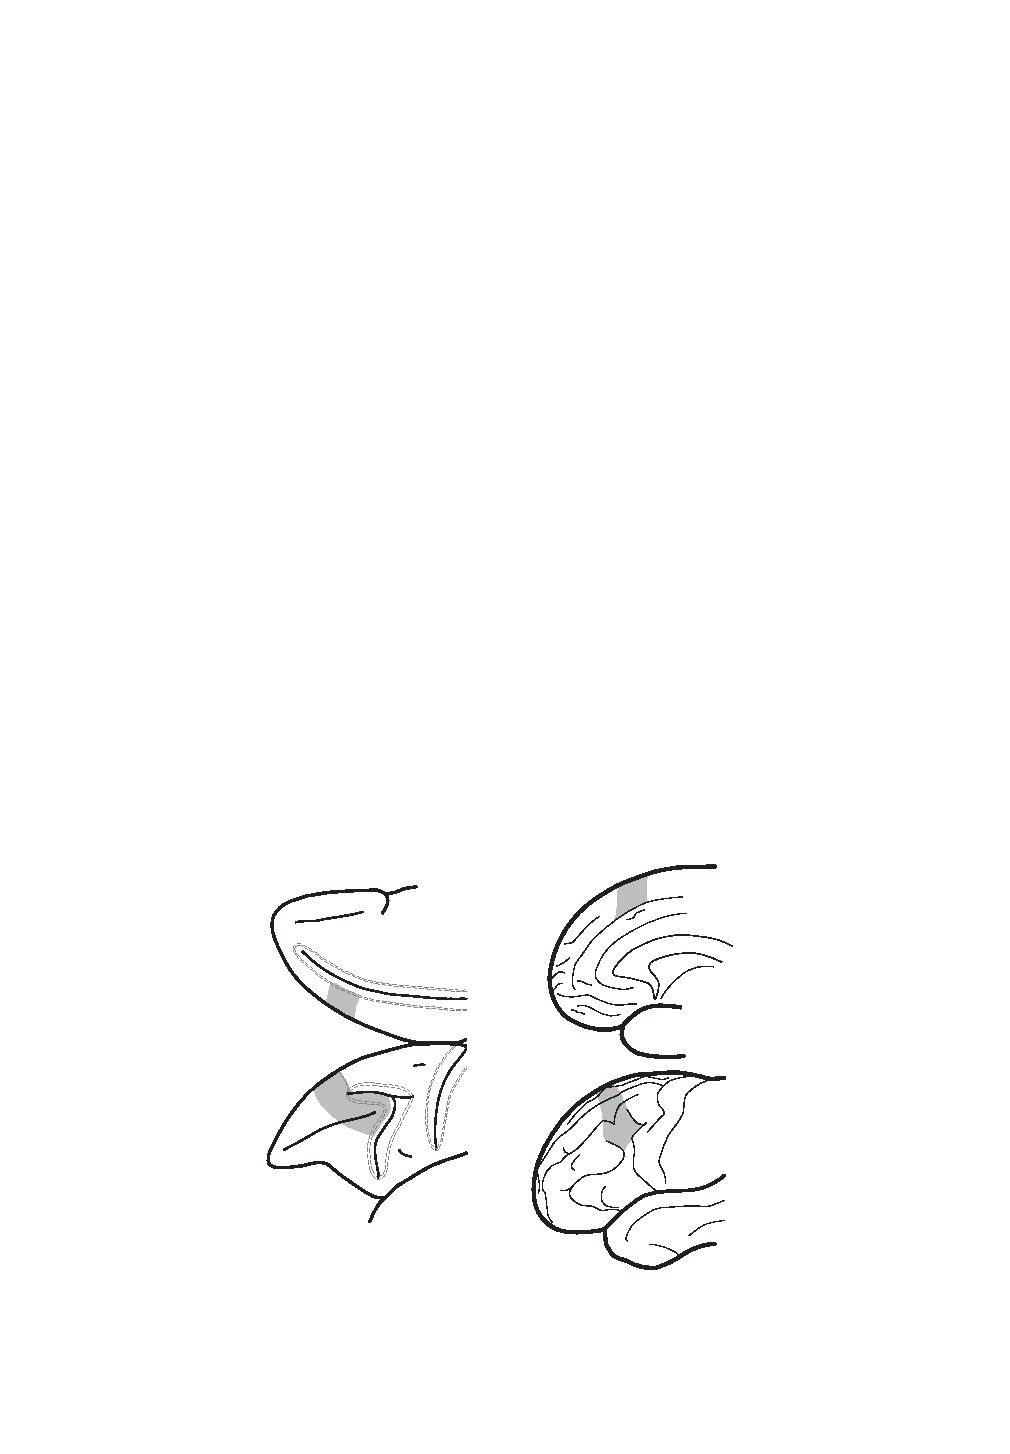
\includegraphics[width=0.7\linewidth]{chap5/Fig_5_1}
	\caption{猕猴(左)和人类(右)的尾侧前额叶皮层。
		格式如图~\ref{fig:1_2}~所示。}
	\label{fig:fig_5_1}
\end{figure}


正如我们所定义的那样,尾侧前额叶皮层总是包括第8区,为了本章的目的,它还包括猕猴主沟的尾侧部分。
我们通过注意到,正如在第8区域\cite{chafee1998matching},主沟尾部的大多数细胞调节其活动与眼球运动相关\cite{tanila1993regional}来证明这一分组是正确的。
Petrides\cite{petrides1999dorsolateral}发现了一个位于主沟尾端附近的区域,他们称之为9/46,他们将该区域与相邻的吻侧中外侧前额叶皮层(46区)和背内侧9区区分开来。
顾名思义,Petrides和Pandya认为9/46区具有与9区和46区相似的细胞结构特性,并且这三个区域都具有颗粒状的细胞结构。
我们称主沟尾侧皮层为后外侧前额叶皮层(图~\ref{fig:1_4}),目前将其包括在前额叶尾侧皮层中。
然而,我们承认,在不违反任何解剖学原理的情况下,可以将其包括在前额叶皮层背侧(第~\ref{chap:chap6}~章)。
表~\ref{tab:1_2}~使用一个查询标记(“?”)来表示这两个选项。
因此,关于后外侧前额叶皮层的许多观点都适用于本章和下一章。


在猕猴中,通过微刺激弓状沟靠近主沟尾端的吻侧岸,可以诱发眼跳运动\cite{bruce1985primate},这一特性定义了额叶视区。
更高的电流可以通过电流传播,从更大的区域唤起跳视\cite{robinson1969eye},但人们普遍认为低阈值区域对应于额叶视区。
因此,区域8包括额叶视区,它从典型的颗粒状细胞结构向非颗粒状细胞结构变化\cite{stanton1989cytoarchitectural}。


Amiez\cite{amiez2009anatomical}回顾了通过电刺激在人脑中定位额叶视区的研究。
来自中央前上沟吻侧的低阈值刺激,以及来自中央前上沟上方的低阈值刺激,可以诱发眼跳。
Amiez等人\cite{amiez2006local}使用成像方法来定位与个体受试者皮层解剖相关的激活峰值。
按照这样的定义,额叶视区始终位于中央前上沟的腹侧分支,这个位置与电刺激所定义的位置大致一致。
Amiez\cite{amiez2009anatomical}提供了猕猴和人类的地图,并表明在这两种情况下,额叶视区都可以与运动前皮层区分开来,电刺激也可以唤起眼球运动。


微刺激还在猕猴的额叶中发现了第二个眼场:\textit{辅助视区}\cite{schlag1987evidence}与额叶视区一样,\textit{辅助视区}中的细胞在扫视前增加活动\cite{hanes1995relationship}。
在猕猴中,\textit{辅助视区}位于背内侧额叶皮层的第6区\cite{schlag1987evidence},它在人脑中有类似的位置\cite{amiez2009anatomical}。



\section{连接}

图~\ref{fig:fig_5_2}~显示了猕猴的尾侧前额叶皮层的皮质连接,包括额叶视区。
这些数据主要来自Petrides\cite{petrides1999dorsolateral},他们将示踪剂注入区域8的细分(区域8B、8Ad或8Av),并描述了它们之间的联系。
这项研究比早期的研究更有优势\cite{petrides1984projections,barbas1988anatomic,barbas1989architecture,cavada1989posterior}进行了小规模和相对选择性的注射。


\begin{figure}
	\centering
	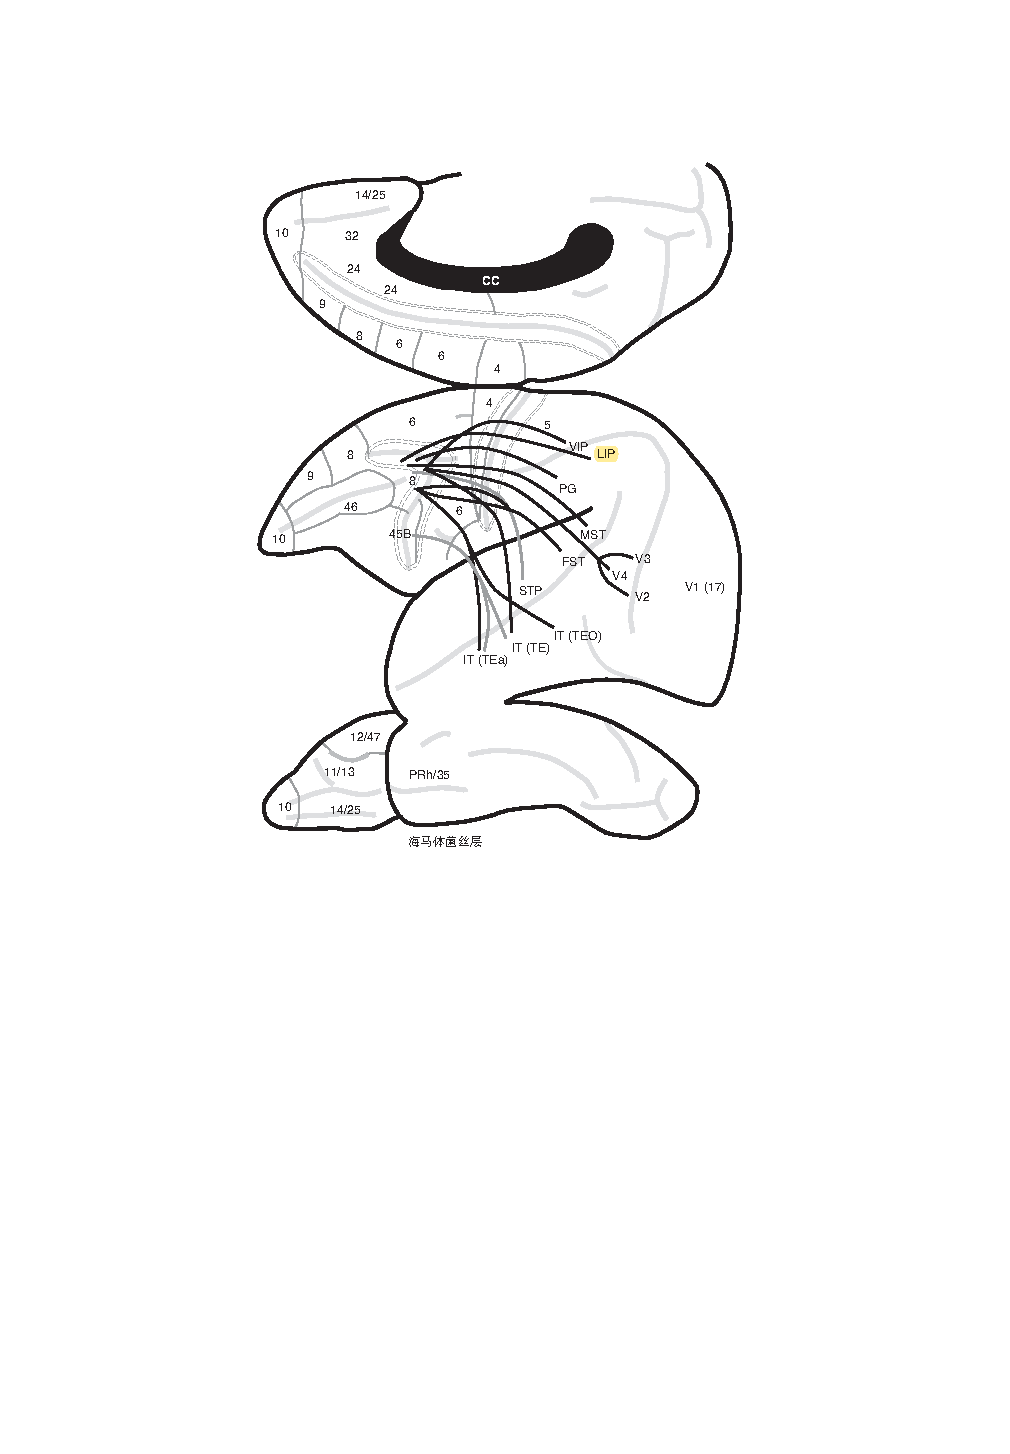
\includegraphics[width=0.7\linewidth]{chap5/Fig_5_2}
	\caption{末梢前额叶皮层的选定连接。
		图~\ref{fig:1_4}和图~\ref{fig:1_5}~给出了沟和区域的名称。
		这些线连接了一些与尾侧前额叶皮质有轴突直接连接的区域,除非另有说明,假设是相互的。}
	\label{fig:fig_5_2}
\end{figure}


根据连接得到以下结论:

\begin{enumerate}
	\item 8Ad区、8B区和后外侧前额叶皮层与执行眼肌运动和视觉空间功能的区域相连。例如,它们与位于顶骨内沟的LIP区有联系\cite{cavada1989posterior,andersen1990corticocortical}, LIP中的细胞编码眼球运动\cite{snyder1997coding}。
	同样的前额叶区域与下顶叶皮层的PG区域有连接\cite{cavada1989posterior},该区域的许多细胞编码眼睛方向\cite{sakata1980spatial}。
	最后,8Ad区与颞区MST区有联系,在MST区,细胞对视觉刺激的运动做出反应\cite{celebrini1995microstimulation}。
	\item 这些视觉区域构成了背侧视觉流的一部分\cite{milner2006visual}(Ungerleider和Mishkin 1982),以区别于腹侧视觉流。
	一般来说,背侧流包括后顶叶区域,处理有关动作空间目标的信息,腹侧流包括颞下区域,处理有关视觉刺激的颜色、形状和纹理的信息。
	\item 额叶视区接收早期(低阶)视觉区域的信息,如枕部视觉区V2和V3\cite{stanton1995topography},但8Ad区和后外侧前额叶皮层不接收信息。
	因此,额叶视区接收到的高度处理视觉信息比前额叶皮层尾端的其他部分和前额叶皮层的其他部分要少。
	\item 8Av区不同于8Ad区、8B区和后外侧前额叶区,分别与腹侧流和背侧流有联系。8Av区与TEO区有联系\cite{webster1994connections},也与颞下皮层的其他部分有联系,如颞上沟下岸的皮层\cite{petrides1999dorsolateral}。
	\item 尾侧前额叶皮层各组成区域之间相互连接紧密。
	8Ad区和8Av区彼此相互投射,并与后外侧前额叶皮层(9/46区)相互投射。
	这些相互联系支持我们将后外侧皮层纳入本章。
	如图~\ref{fig:1_8}~所示,我们所定义的尾侧前额叶皮层与Price\cite{price2010neurocircuitry}所定义的尾侧网络非常相似。
\end{enumerate}



图~\ref{fig:fig_5_2}~和前面的列表涉及皮质连接,但尾侧前额叶皮层的皮层连接也解释了其功能的一些重要内容:


\begin{enumerate}
	\item 额叶视区\cite{kunzle1976projection,huerta1986frontal}、8区其余部分\cite{fries1984cortical}和后外侧前额叶皮层\cite{selemon1988common}都向上丘发送直接投影。
	在所有脊椎动物中,上丘及其同源体都有定位头部感受器的功能。
	因此,这些皮质连接指向了尾侧前额叶皮层在控制眼球运动方面的作用,但大脑皮层的许多其他部分也投射到上丘\cite{leichnetz1981prefrontal,fries1984cortical},所以这种解剖特征并不能将前额叶皮层与其他区域区分开来。
	\item 额叶视区还可以通过向基底神经节的投射影响上丘的活动。
	额叶视区投射到尾状核的内侧\cite{stanton1988frontal},后者又投射到黑质网状部\cite{hedreen1991organization}。
	该核投射到上丘,在那里发挥抑制作用\cite{hikosaka1985modification}。
	\item 最后,额叶视区直接投射到脑干动眼肌核\cite{segraves1992activity,yan2001overlap}。
\end{enumerate}



\subsection{总结}

尾侧前额叶皮层的连接指纹表明,它接受直接的、较低的视觉输入,它具有与背侧视觉流和腹侧视觉流平行的背侧-腹侧差异,并且它通过基底神经节到上丘的投射直接或间接地输出到动眼神经核。



\section{额叶视区是前额叶区域}

尽管有输出表明额叶视区在控制眼球运动中起作用,但我们并不认为额叶视区主要在眼球运动控制中起作用。
我们知道,当药物抑制额叶视区时,视觉引导的扫视在被引导到对侧空间时变得不准确\cite{sommer1997reversible}。
在这个意义上,额叶视区类似于前运动皮层。
例如,腹侧前运动皮层的失活会导致肢体运动不准确\cite{kurata1994differential}。


我们也知道额叶视区的永久性损伤不会消除眼跳运动,就像前运动皮层病变不会消除肢体运动一样。
然而,一个原因是除了其他区域外,\textit{辅助视区}\cite{huerta1990supplementary}和顶叶区域LIP\cite{holloway2002brief}也向上丘发送投射。
因此,为了消除眼跳,需要同时去除上丘和额叶视区\cite{schiller1979effects,schiller1987effect}。
只剩下最小的扫视。


然而,尽管有这些运动功能的证据,我们认为额叶视区是前额叶区域,而不是运动前区域。
我们这样做是因为我们区分了产生、发现和关注目标的机制和实现目标的机制。
记住,我们所说的目标指的是对象或地点,而不是奖励或结果。
实现目标的行动会产生结果。
除了在实验室,视觉注视和注意力永远不会产生这种意义上的结果。
在野外,看着或吃着一种食物并不会产生任何营养或补水的好处。
实现这一预期结果需要其他机制。
我们认为前者是前额叶皮层的功能,后者是前运动皮层的范围。


Shadmehr\cite{shadmehr2004computational}在他们对前运动皮层的治疗中提出,它处理的是视运动转换,将伸手运动的视觉目标转换为关节角度和力的变化,从而驱动手到达这些目标。
第~\ref{chap:chap2}~章提到了这种机制。
详细信息可以在Shadmehr和Wise中找到,但这里有一个简短的总结。


假设有人伸手拿咖啡杯。
基本上,运动系统需要建立两个位置:目标位置和手的初始位置。
Shadmehr和Wise提出后顶叶和前运动皮层的细胞在一个坐标框架中编码这些位置,在其原点,视觉注视点。
然而,在理论上,任何视网膜坐标都可以作为原点。
图~\ref{fig:5_3}~显示了这种机制是如何工作的。
图中显示了两个向量:一个是尾部在注视点,尖端在运动目标处;
另一种是尾部在固定点,尖端在手的当前位置。
两个向量的简单相减就得到了一个向量,它的尾部在手上,顶端在目标上。
这个计算的结果相当于一个“运动计划”,将视觉参考系转换为以手为中心的坐标系。
前运动区和初级运动区,连同皮层下结构,将这个矢量转换成关节角度的变化和使这个运动的力量。


\begin{figure}
	\centering
	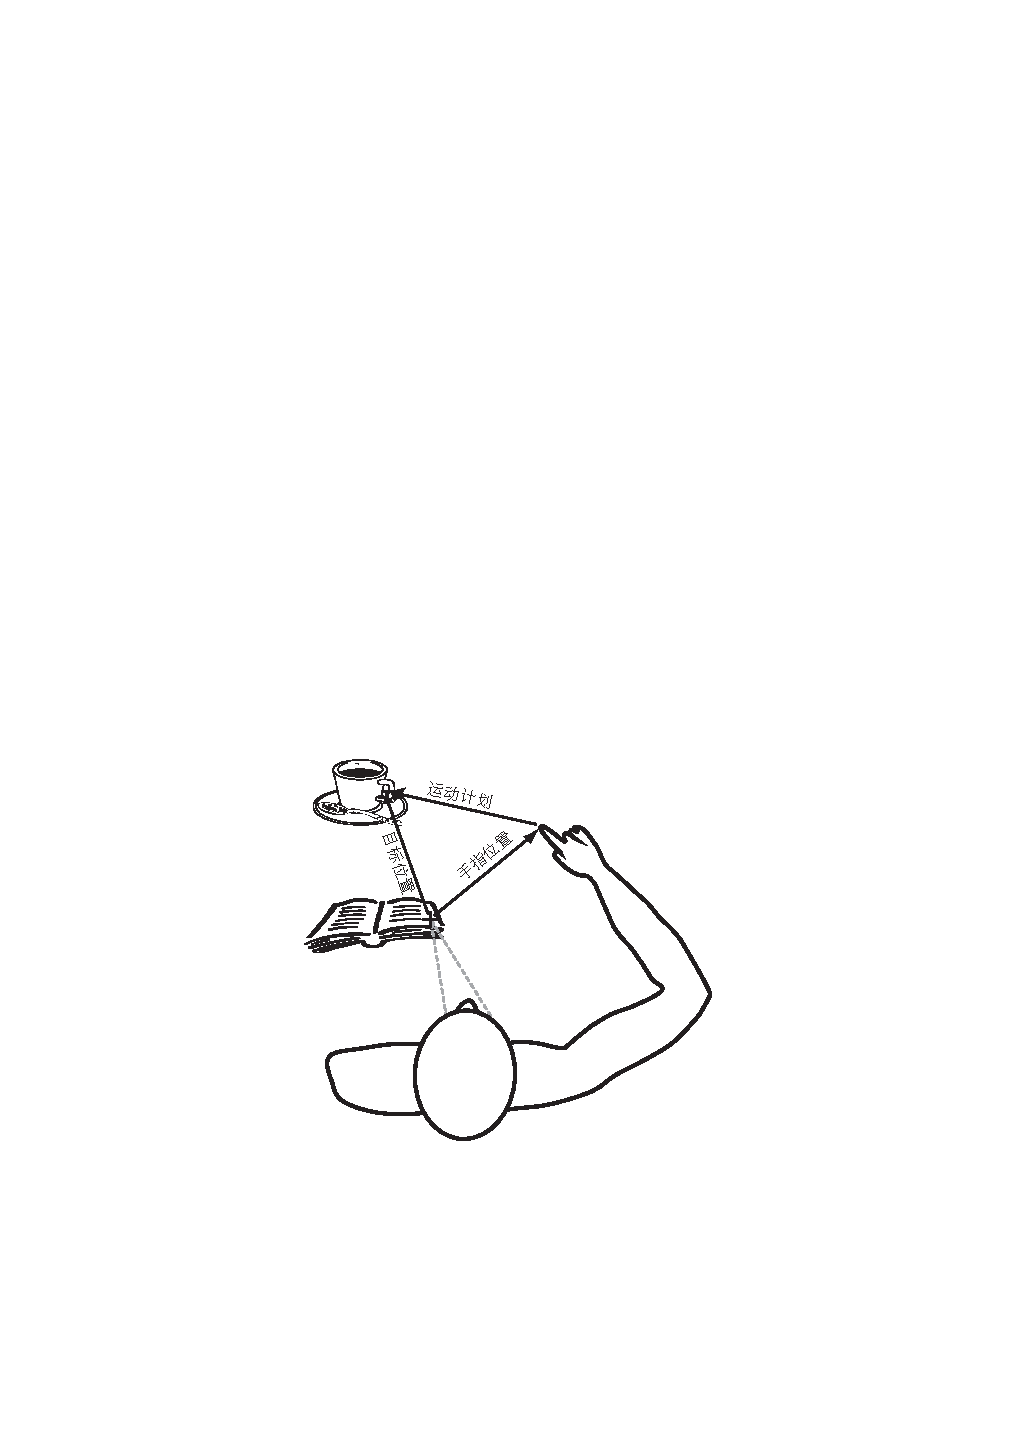
\includegraphics[width=0.55\linewidth]{chap5/Fig_5_3}
	\caption{运动平面的矢量表示。
		这个人的目标是把他的指尖穿过咖啡杯的把手。
		他或她制定了一个读书计划。
		“+”标志着他当时的注视点。
		来自注视点的两个向量编码目标的位置和手指在非中心的外部坐标框架中的当前位置:注视中心坐标。
		两个矢量之间的差表示以手为中心坐标的电机平面\cite{shadmehr2004computational}。}
	\label{fig:5_3}
\end{figure}


通过这种机制或类似的机制,前运动区和后顶叶区以一种眼球运动或其他形式的注意力都无法实现的方式实现目标。
在我们的例子中,这个人想要咖啡,所以把他或她的注意力转移到杯子上。
注意力可以是显性的(即中央凹朝向杯子),也可以是隐性的(即只关注杯子而不看它)。
杯子里的东西与人当前的需求有关,因此他或她产生了一个目标(咖啡杯),然后搜索并将注意力转移到杯子上。
我们认为,尾侧前额叶皮层执行搜索和注意功能。
虽然视觉固定和注意力不能达到预期的结果,但伸手到杯子里,把它送到嘴里,从里面喝水就可以了。
我们将后一种功能视为前运动区和初级运动区,以及运动系统的其他部分。


那么,有什么证据表明额叶视区参与了对目标的寻找和关注,而不是实现目标的手段?
我们已经看到,与运动前区域不同,额叶视区接收来自低阶视觉区域的直接输入,特别是枕叶和颞叶皮层称为V2、V3、V4和MST的区域\cite{stanton1995topography}。
这些联系解释了为什么额叶视区中的一些细胞在感觉刺激出现后表现出活动增加,而在运动之前却没有\cite{schall1991neuronal}。
它们似乎明确了视觉目标,而不是注视这些目标所需的眼球运动。
此外,在顶叶区LIP投射到额叶视区的细胞中,78\%有视觉反应,但没有扫视相关活动\cite{ferraina2002comparison}。
这种投影可以提供另一种关于视觉目标的信息来源,而且是独立于运动指令的信息来源。


当然,额叶视区中的许多细胞具有视觉运动活动:它们在视觉目标出现时和眼球运动之前调节自己的活动\cite{schall1991neuronal}。
其中很多都是在刺激出现后不久,即刺激引起注意时,指定刺激的位置。
Sato\cite{sato2003effects}教猴子在一系列干扰物中发现一个视觉弹出刺激,然后对该位置进行扫视(prosaccade试验)或对相反方向的扫视目标进行扫视(反扫视试验)。
如果活动反映了刺激的位置,那么两种试验类型的活动应该是相同的。


Sato和Schall比较了两项任务中额叶视区细胞的活动,当弹出的刺激落入细胞的接受野时。
对于反眼跳任务,注意当弹出刺激这样做时,眼跳目标是在相反的方向。
然而,57\%的任务相关细胞的活动最初反映了刺激的位置,尽管随后86\%的这些细胞后来编码为扫视目标。


这些结果表明,额叶视区中的细胞活动可以反映刺激的位置,独立于运动,并且这种活动反映了隐蔽注意的方向。
与这一观点一致,Armstrong\cite{armstrong2007rapid}表明,额叶视区的皮层内微刺激增强了视觉区V4(腹侧视觉流的中层区域)的细胞响应。
它是专门为视觉空间的一个特定部分做的。
刺激额叶视区的效果可能模仿了猴子在该位置秘密关注物体时所发生的情况。


如果额叶视区真的在隐性注意和显性注意中起作用,该区域的暂时失活应该会导致对中央凹外刺激的注意受损。
因此,Wardak等\cite{wardak2004deficit}教猴子在干扰物中发现目标,而动物则保持对中心光点的固定。
在额叶视区失活后,猴子发现周围目标的速度很慢。
Iba\cite{iba2003involvement}表明,失活也会导致猴子对目标进行扫视的速度变慢。
这些发现表明,额叶视区在对刺激的公开注意和隐蔽注意中都有作用,特别是当这些刺激作为后续行动的目标时。


这一观点与第~\ref{chap:chap2}~章中关于前额叶进化的描述非常吻合。
Strepsirrhine灵长类动物没有中央凹,早期灵长类动物可能也没有。
因为包括额叶视区在内的尾侧前额叶皮层在早期灵长类动物中进化而来,它一开始不可能与中央凹或中央凹有任何关系。
所以,从这个意义上说,这些动物的所有视觉都对应于中央凹外视觉,所有的注意力都是隐蔽的。
顺畅的眼球运动可以让类人猿灵长类动物锁定中央凹,将注意力集中在移动的物体上,并保持高分辨率图像。
但这种能力也可能在缺乏中央凹的灵长类动物中进化而来\cite{shepherd2009neuroethology}。
因此,从中央凹视觉或明显的注意力来解释灵长类动物的前额叶皮层的起源是错误的,尤其是尾侧前额叶皮层的起源。


然而,中央凹最终在后来的灵长类动物中进化出来,现代眼镜猴、猴子、猿和人类(单足纲)通过遗传拥有它。
尽管有很多优点,但集中注意力的能力是有代价的。
那视觉世界的其余部分呢?
这个混乱的世界还包含许多其他突出的项目。
在某种意义上,没有中央凹的视网膜提供了一个更平衡的世界观。
即使在中央凹进化之后,保持隐蔽注意力的好处是,它可以增强对有限数量的中央凹外物体的处理,即使最密集的处理是用于中心凹的物体和地方。
隐蔽注意力和搜索的重要性在于,所有被关注的对象,而不仅仅是被聚焦的对象,都可能成为未来行动的目标。
根据这一观点,包括额叶视区在内的尾侧前额叶皮层进化为隐蔽的搜索和注意力,但后来一旦中央凹出现,就适应了公开的注意力。



\subsection{总结}

许多神经科学家将额叶视区视为眼球运动区域,并将其视为眼球运动的前运动区域。
我们提出一个不同的想法。
我们将额叶视区和尾侧前额叶皮层的其他部分视为前额叶区域,而不是前运动区域,并提出它们在寻找和关注灵长类动物重要目标方面发挥作用。
在许多灵长类动物中,包括猴子和人类,对目标的关注通常意味着眼球运动,使中央凹朝向目标(扫视)或在目标移动时保持视觉固定(平稳跟踪)。
但是隐蔽的注意力也扮演着重要的角色,在缺乏中央凹的早期灵长类动物中,它肯定是这样的。
由于注视是注意力的一种形式,我们将眼球运动视为一种注意力功能,而不是一种运动功能。
我们提出,包括额叶视区在内的尾侧前额叶皮层的功能是将公开或隐蔽的注意力引向一个目标,而不是作为实现目标的机制的一部分。



\section{动眼肌延迟响应任务}

我们将额叶视区与尾侧前额叶皮层的其余部分分开处理,因为额叶视区皮层内微刺激会引起眼球运动。
但是,正如在连接部分所解释的那样,额叶视区与尾侧前额叶皮层的其他部分有紧密的连接。
因此,8区\cite{chafee1998matching}和后外侧前额叶皮层\cite{funahashi1989mnemonic}的许多细胞具有与眼球运动相关的活动。


正如我们前面所说的,后外侧前额叶皮层的连接使我们在本章中将其与包括额叶视区在内的后外侧前额叶皮层一起考虑。
我们在第~\ref{chap:chap2}~章中对皮层进化的讨论为这种方法提供了一些可信度,后外侧前额叶皮层中存在编码眼球运动的细胞。
由于后外侧前额叶皮层(9/46区)处于中间状态,在本节中,我们将讨论在第~\ref{chap:chap6}~章中再次出现的主题,最显著的是被称为“空间记忆任务”的任务中的延迟期活动问题。
我们这样做主要是为了方便,并认为没有什么关键取决于我们是否将后外侧前额叶皮层与尾侧前额叶皮层组或背侧前额叶皮层组进行分类。


动眼力延迟响应任务在包括后外侧前额叶皮层在内的尾侧前额叶皮层的研究中发挥了突出作用。
它不同于经典的延迟响应任务,因为猴子通过扫视而不是到达一个空间目标来选择潜在的目标。


\begin{figure}
	\centering
	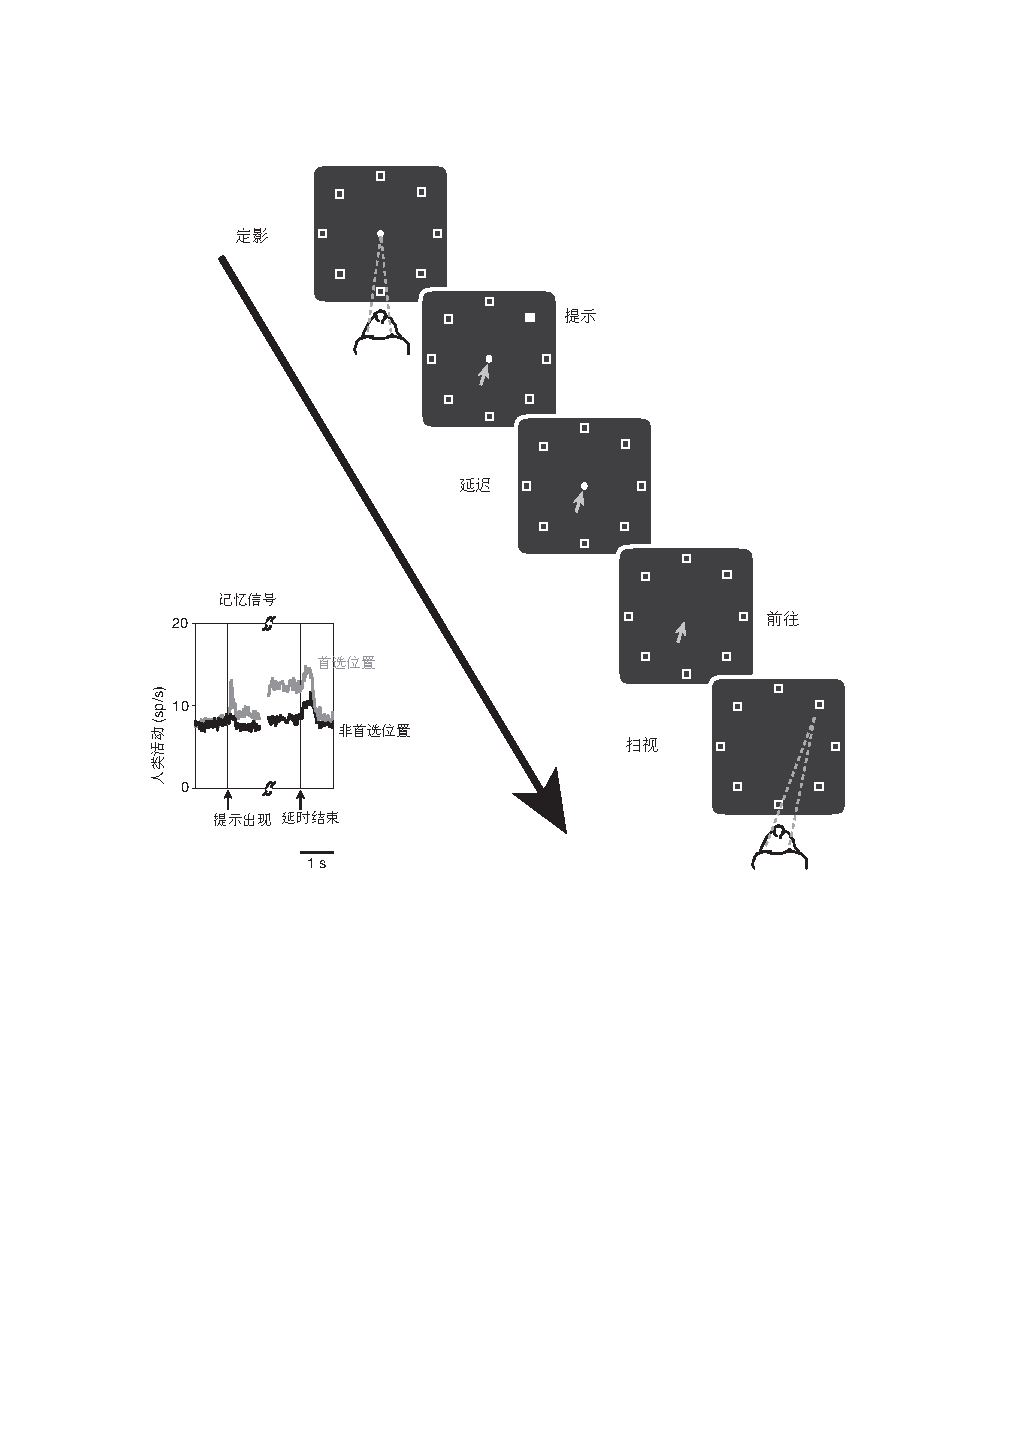
\includegraphics[width=0.75\linewidth]{chap5/Fig_5_4}
	\caption{普通版本的动眼器延迟响应任务。
		在试验过程中,每个面板在不同的时间显示屏幕,在其他试验中,未填充的白色方块是潜在的空间目标。
		填满的白色方块表示一个例子试验的线索,填满的白色圆圈表示注视点。
		灰色虚线和灰色箭头表示猴子的注视点。左下方的插入图显示了空间记忆信号,由Lebedev等人\cite{lebedev2004representation}从前额叶皮层细胞群中记录,灰色为首选记忆位置的平均活动,黑色为反首选位置的平均活动。
		因为Lebedev等人控制了注意力,这些数据代表了前额叶皮层空间记忆信号的最有力证据,尽管它们只出现在延迟期间编码位置的少数细胞中。}
	\label{fig:fig_5_4}
\end{figure}


动眼肌延迟反应任务有三个阶段:提示、延迟和选择(图~\ref{fig:fig_5_4})。
在第一阶段,一个视觉空间线索会短暂地出现在受试者视野的某个地方。
这个刺激指示了猴子必须扫视的位置,但直到延迟期结束,猴子必须继续盯着一个中心光点。
在一段从几百毫秒到几秒不等的延迟时间后,一个“开始”信号告诉受试者将扫视移动到最近提示的位置。
如果被试的扫视准确,就会得到奖励。


尽管实验人员可以使用任何提示位置的配置,但常见的版本包括以注视点为中心等距排列的八个显著位置,如图~\ref{fig:fig_5_4}所示。
该图将位置显示为空方格,并表示球杆为填充方格。
然而,重要的是要注意,正如通常所呈现的那样,外围位置没有以任何方式标记,这意味着当猴子响应“go”信号时,它会扫视到屏幕上未标记的位置。


在这项任务中,尾侧和后外侧前额叶的许多细胞表现出延迟期活动\cite{chafee1998matching}。
图~\ref{fig:fig_5_4}~显示了Lebedev等人\cite{lebedev2004representation}在种群水平上从尾侧前额叶皮层记录的记忆信号。


Funahashi和他的同事\cite{funahashi1989mnemonic,takeda2002prefrontal}展示了他们的电极穿透皮层的位置映射,我们假设这些细胞延伸到整个采样区域。
Lebedev等人的研究表明,具有记忆特异性信号的细胞位于主沟尾端9毫米处,主要位于主沟背侧及其附近。
Chafee\cite{chafee1998matching}报告说,延迟期活动主要来自8A区,但他们的图表显示,一些细胞也来自后外侧前额叶皮层。


成像实验在类似领域也得到了结果。
Inoue等\cite{inoue2004functional}比较了眼肌运动延迟反应任务中的眼跳激活与猴子对屏幕上标记的位置进行眼跳的任务中的激活。
差异激活位于后外侧前额叶皮层和8区,包括额叶视区。


鉴于以下事实,这是一个重要的观察,下一章将解释,在经典的、达到版本的延迟响应任务上的表现取决于中外侧前额叶皮层,而不是尾侧前额叶皮层。
因此,动眼肌延迟响应任务不同于经典的延迟响应任务,基于动眼肌版本任务的结论不一定适用于经典的延迟响应或延迟交替任务。
后外侧前额叶损伤对这些任务的经典版本缺乏影响\cite{butters1969retention},这强化了这样一种观点,即该区域在目标的寻找和关注中发挥作用,而不是在目标的实现(前运动皮层功能)或目标的产生(背侧前额叶皮层功能,如第~\ref{chap:chap6}~章所述)。


\begin{figure}
	\centering
	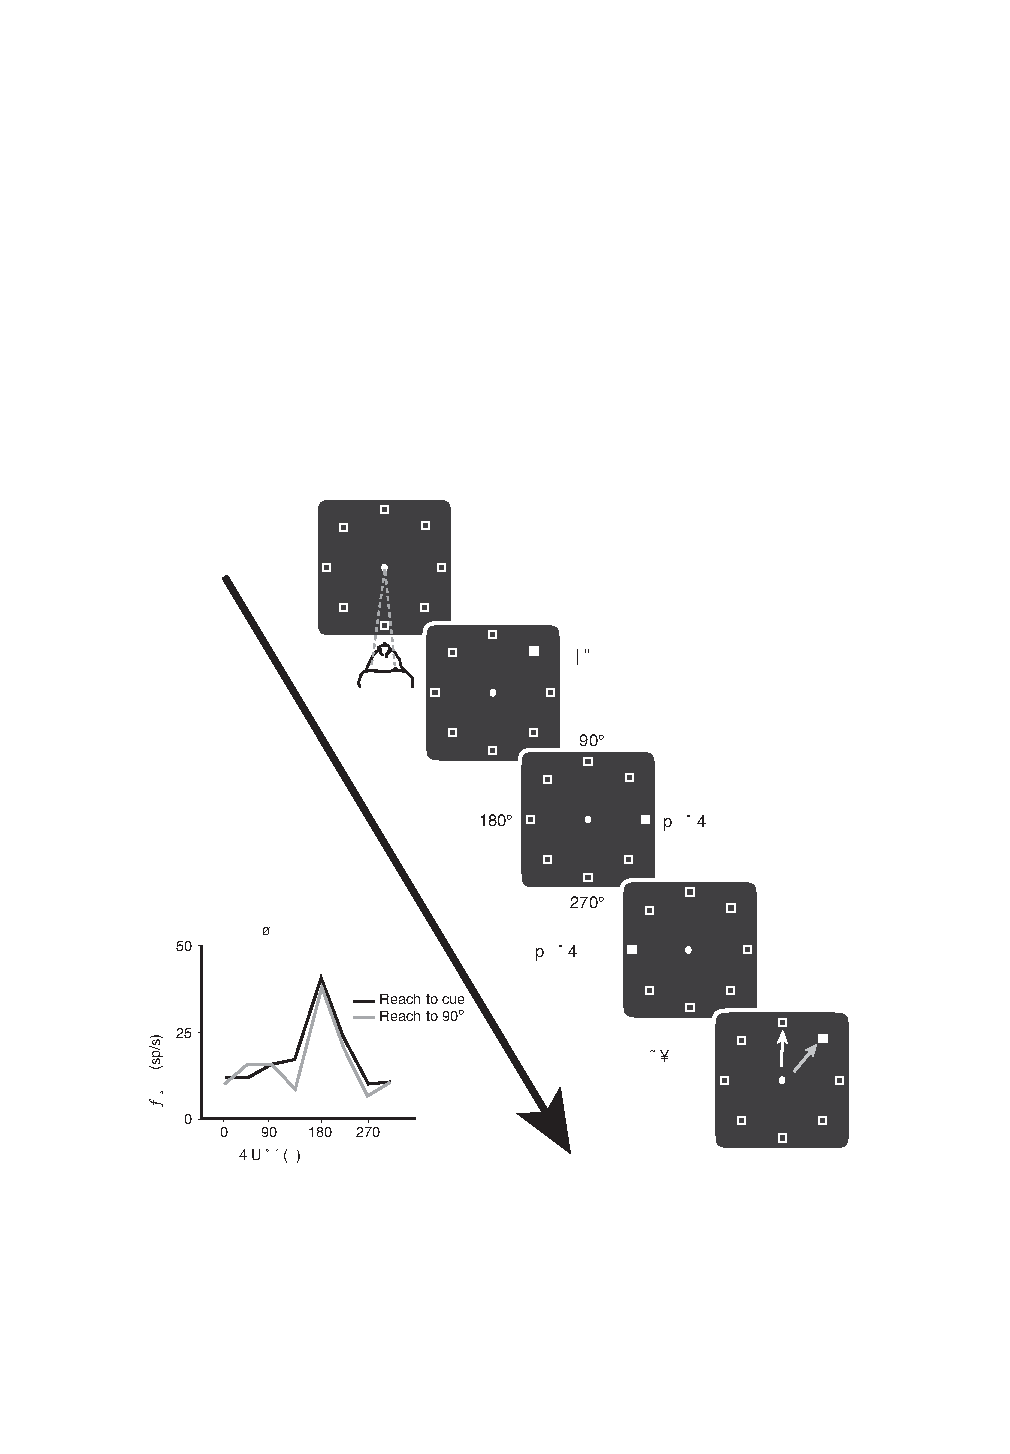
\includegraphics[width=0.75\linewidth]{chap5/Fig_5_5}
	\caption{di Pellegrino\cite{di1993visuospatial}使用的空间匹配样本任务。
		格式如图~\ref{fig:fig_5_4}~所示。
		在底部面板上,箭头表示在两种情况下达到运动的目标。
		在一种情况下,提示的位置是伸手动作的目标;
		在另一种情况下,无论球杆的位置如何,90°的位置(图中向上)始终是到达目标。
		左下方的插图显示了前额叶皮层中一个细胞的活动,该细胞在延迟期间编码最左边的线索(180°),在两种情况下都是一样的。}
	\label{fig:fig_5_5}
\end{figure}


\subsection{解释延迟期活动}

传统的解释是,眼肌运动延迟响应任务中的延迟期活动,就像延迟响应任务的标准版本一样,反映了回溯性空间工作记忆。
根据这种观点,这种活动反映了在短期记忆中线索位置的维持。
这种解释部分来自于将该任务称为“空间记忆任务”,并因此假设在延迟期间发生的主要认知过程是感官信息的维持。
事实上,这种观点的支持者经常把延迟期称为“记忆期”。
但是,第~\ref{chap:chap1}~章警告不要接受任务的名称。
事实上,在延迟期间还会发生其他过程,包括对提示位置的隐蔽注意和运动的准备。


有几种方法可以区分这些可能性,我们将它们进行了编号:


\begin{enumerate}
	\item 我们可以比较动眼肌延迟响应任务的两个版本。因此,Funahashi等人\cite{funahashi1993prefrontal}比较了一个版本,其中猴子必须对目标进行扫视(prosaccade),
	另一个版本中猴子必须对距离线索180°的位置进行扫视(反扫视)。
	在后来的一项研究中,Takeda\cite{takeda2002prefrontal}比较了标准的动眼肌延迟反应任务和猴子必须以90°的角度扫视该位置的条件。
	这些实验有如下逻辑:如果延迟期活动编码了线索在记忆中的位置,那么无论运动的目标是什么,它都应该是相同的。
	在这两项研究中,大多数与任务相关的细胞反映了线索的位置,尽管有相当一部分反映了目标的位置。
	Funahashi等人报告说,51个与任务相关的细胞中有31个(61\%)编码了线索的位置,而这51个细胞中有13个编码了目标的位置。
	尽管细胞样本很小,但这些发现使作者得出结论,延迟期活动反映了对提示位置的记忆。
	\item 第二种方法试图排除这种可能性,即通过使用单一的、重复的手部运动来报告线索的位置,而不是移动到该位置,从而对非感官因素进行编码。
	Sawaguchi\cite{sawaguchi1999properties}使用了这种方法。他们在延迟期后呈现一个空间视觉线索,并要求猴子只有在与线索位置匹配的情况下才释放杠杆。
	读者会认为这是匹配样本任务的空间版本。
	在与任务相关的神经元中,48\%显示出延迟期活动,这些细胞中90\%编码了提示位置。
	这些结果也被用来支持延迟期活动在空间记忆方面的解释。
	\item 正如di Pellegrino\cite{di1993visuospatial}所做的实验那样,上述两种方法可以结合起来。
	实验设计如图~\ref{fig:fig_5_5}~所示。
	在Sawaguchi\cite{sawaguchi1999properties}的实验中,猴子需要报告延迟期结束时的线索是否与延迟前出现的线索的位置相匹配。
	然而,猴子以不同的方式报告匹配的刺激,如图~\ref{fig:fig_5_5}~底部的两个箭头所示。
	这种报告要求从一个试验块到下一个试验块交替进行。
	在一个街区,猴子向提示的位置移动。
	在下一个街区,不管线索和匹配的刺激出现在哪里,猴子都到达一个固定的位置。
	有时,提示方向和报告方向之间的夹角等于180°,如Funahashi等人\cite{funahashi1993prefrontal}的反眼跳任务,有时等于90°,如Takeda\cite{takeda2002prefrontal}的实验。
	
	Di Pellegrino和Wise记录了尾侧和后外侧前额叶皮层,并发现,与Funahashi等人一样,无论运动的目标如何,61\%的细胞具有相同的延迟期活动(图~\ref{fig:fig_5_5})。
	这一结果也可以表明,细胞的活动编码了对提示位置的记忆。
	\item 所有这些研究都基于这样一个假设:只有两个重要因素是线索的位置和移动目标的位置。将延迟期称为“记忆期”,人们很容易忽略另一种可能性,即与记忆一样,延迟期也涉及注意力:有时是显性的,有时是隐性的。
	为了测试这种可能性,Lebedev等人\cite{lebedev2004representation}引入了一种新的实验设计,如图~\ref{fig:fig_5_6}A~所示。
	正如第~\ref{chap:chap1}~章所提到的,他们教猴子记住一个空间位置,并秘密地注意到另一个位置,同时这样做。
	
	Lebedev等人记录了尾侧和后外侧前额叶皮层的细胞活动。
	在对空间位置进行编码的任务相关细胞中,大多数(61\%)选择性地对参与的位置进行编码,而不是对记忆中的位置进行编码。
	少数(16\%)细胞选择性地编码记忆位置,其他细胞具有中间属性(图~\ref{fig:fig_5_6} B)。
	注意信号在每个测量中都超过了记忆信号(图~\ref{fig:fig_5_6} C)。
	\item 如果大多数细胞反映隐蔽注意力,那么当受试者需要参加某个地方,但不需要记住这个位置时,就应该有可能证明激活。
	成像可以用来检验这一预测。
	Astafiev等\cite{astafiev2003functional}提示受试者在保持中心注视的同时注意左边或右边。他们报告了额叶视区的激活,以及在顶骨内沟附近的后顶骨区域。
	
	Curtis\cite{curtis2006selection}进行了类似的成像研究,但有两次延迟。
	他们的实验对象看到了即将到来的扫视的几个潜在目标,随后是第一个延迟期,在此期间,实验对象需要记住这些地方。
	在第一次延迟期间,额叶视区和后顶叶皮层都发生了持续的激活。
	然后出现了一个箭头,指示在该试验中哪个目标应该是眼球运动的目标。
	第二次延迟后,受试者按指示进行扫视。
	在第二次延迟期间,持续的激活只发生在额叶视区,而不是在后顶叶皮层。这一发现与中央凹是一种注意力功能的观点一致。
	包括额叶视区在内的尾侧前额叶皮层,在将注意力导向潜在目标方面发挥作用,这在两次延迟期间都发生过混乱,不仅仅是在记忆位置上,发生在第一次延迟的时候。
\end{enumerate}


\begin{figure}
	\centering
	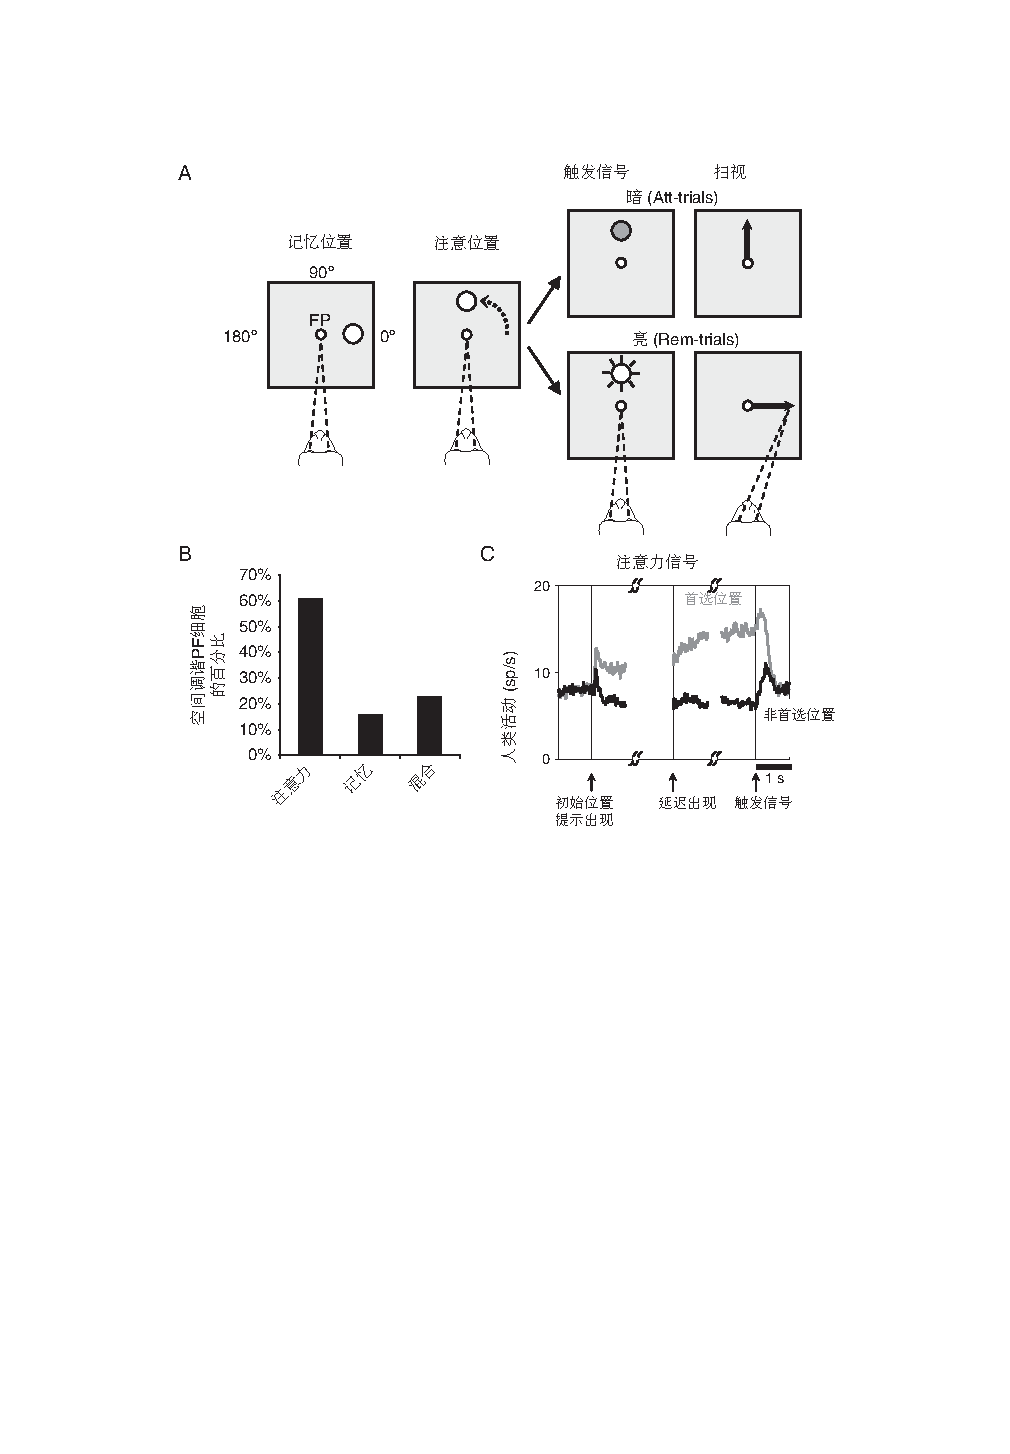
\includegraphics[width=0.7\linewidth]{chap5/Fig_5_6}
	\caption{前额叶皮层的注意力和记忆编码。
		(A)任务设计。视频监视器上出现一个圆(灰色矩形),随后开始围绕中心注视点(FP)旋转。
		它从四个位置中的一个开始,然后停在相同的四个位置中的一个:从中心向上、向下、向左和向右。
		如果圆圈变暗(上叉),猴子需要在这次试验中扫视圆圈的最终位置;如果它变亮了(底部的叉子),猴子必须在这次试验中向圆圈的初始位置扫视。箭头表示在两种情况下正确的扫视。
		缩写:Rem,记忆位置;丙氨酸,attended-location。
		(B)空间调谐的前额叶皮层神经元编码参与或记忆的位置或两者(混合)的百分比。
		(C)注意信号格式为记忆信号,如图~\ref{fig:fig_5_4}~所示\cite{lebedev2004representation}。}
	\label{fig:fig_5_6}
\end{figure}


我们得出结论,在这些实验中,延迟期活动或激活有几种可能的解释。
它可以反映对提示位置的记忆,对该位置的隐蔽注意力,或将公开注意力引导到该位置的准备。
此外,它还可以反映任务规则的编码,这是我们将在下一章讨论的主题。


因此,动眼肌延迟反应任务延迟期间的活动并没有显示任何关于回顾性空间工作记忆的内容。
首先,这种活动反映的是隐蔽注意力,而不是感官记忆。
第二,工作记忆的概念没有区分位置的回顾编码和前瞻性编码。
正如我们在下一章所解释的那样,前瞻性编码一词指的是对选定目标的短期记忆。
尽管一些实验,如Funahashi等人的反眼跳任务,试图排除目标位置的预期编码,但在每种情况下,都有相当数量的少数细胞编码目标。
将空间注意力与空间记忆进行对比的实验表明,前额叶皮层的大部分活动编码的是隐蔽参与的位置,而不是被记住的位置。
我们将在第~\ref{chap:chap6}~章和第~\ref{chap:chap7}~章回到前瞻性编码的主题。



\subsection{中断延迟期活动}

不管对延迟期活动的正确解释如何,中断它都会造成某种程度的损害。
然而,简单地表明,在尾叶前额叶皮层有损伤的猴子在一项任务中表现得很差,并不能证明它们这样做是因为它们不再记得提示的位置。
这也可能表明他们很难注意到提示的位置或在记忆中保持它的预期代码。


受试者在动眼肌延迟反应任务中可能会犯两种类型的错误。
Frank误差涉及错误的空间目标的选择\cite{keller2008effect},而精度误差涉及更接近正确目标而不是任何其他可能目标的移动,但错过了其确切位置。


不准确的扫视可能反映了低水平的运动障碍,因此需要将缺乏延迟期的控制条件与标准任务进行比较。
在这里,受试者只是对一个可见的目标进行扫视。


猴子的额叶视区失活会引起低视眼跳。
也就是说,对可见位置的扫视往往达不到空间目标\cite{dias1999muscimol}。
低眼跳也发生在额叶视区单侧病变的患者中\cite{gaymard1999frontal,ploner1999errors}。


冷却导致8A区失活也会导致眼球运动延迟反应任务的不准确扫视。他们往往达不到正确的目标位置,或在目标位置的一侧\cite{chafee2000inactivation}。
用肌西酚\cite{sawaguchi2001prefrontal}或多巴胺拮抗剂\cite{sawaguchi1991d1}灭活后外侧前额叶皮层具有同样的效果。
后外侧前额叶皮层的单侧消融也是如此\cite{funahashi1993dorsolateral}(图~\ref{fig:fig_5_7})。


尽管额叶视区、尾侧前额叶皮层的其他部分或后外侧前额叶皮层的失活会导致不准确的扫视,但这些扫视通常朝着正确的方向前进,并在更接近提示位置的地方结束,而不是任何其他目标。
然而,Funahashi等人\cite{funahashi1993dorsolateral}得出结论,这些眼跳的不准确反映了回溯性空间工作记忆的失败。


他们从未解释过,如果猴子不记得目标位置,它们的扫视最终会更接近提示的位置,而不是任何其他潜在的目标位置。


\begin{figure}
	\centering
	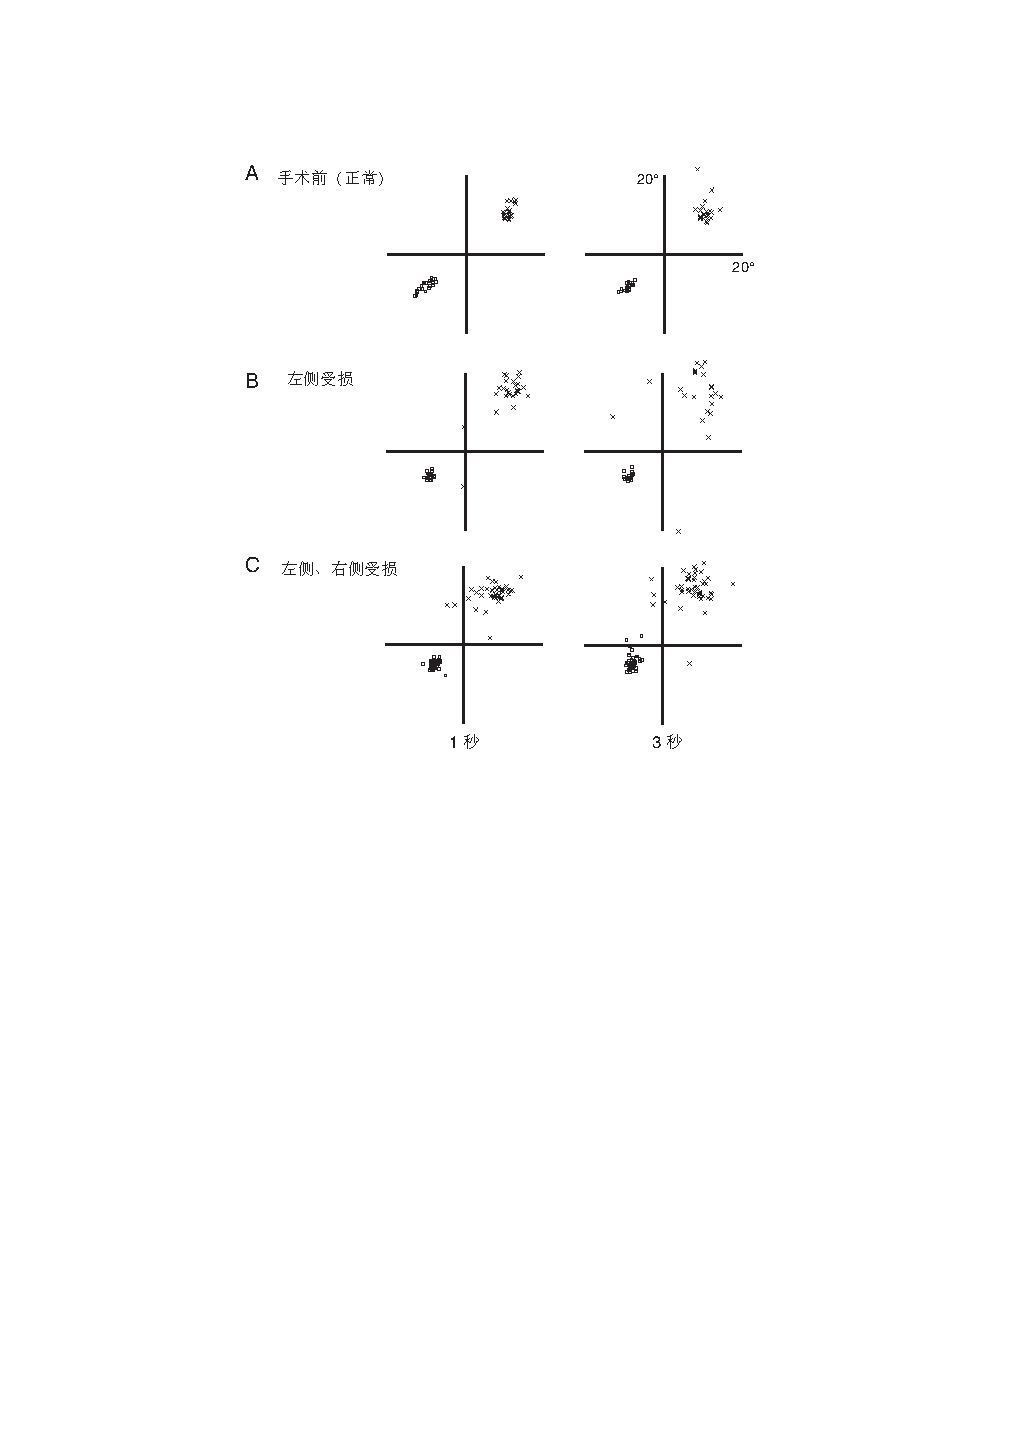
\includegraphics[width=0.67\linewidth]{chap5/Fig_5_7}
	\caption{一只猴子在动眼力延迟反应任务上的表现。
		(A)术前(正常)表现正方形表示225°(向下和向左)目标的扫视终点;十字表示45°(向上和向右)的目标。
		(B)左半球后外侧前额叶皮层单侧损伤后的表现。
		(C)右半球同一区域额外病变后的表现,以完成双侧病变。
		底部的延迟持续时间\cite{funahashi1993dorsolateral}。}
	\label{fig:fig_5_7}
\end{figure}


工作记忆解释的支持者可能会争辩说,猴子之所以不会犯明显的错误,是因为这些损伤,无论是永久性的还是暂时性的,都是单方面的。
毕竟,我们知道在标准延迟反应任务中,中外侧前额叶皮层的单侧损伤只会引起轻度损伤\cite{rosen1975effects},而双侧损伤后的损伤是严重的\cite{goldman1971analysis}。
因此,Funahashi等人\cite{funahashi1993dorsolateral}在两只猴子身上进行了双侧损伤,并分两个阶段进行。
图~\ref{fig:fig_5_7}~显示了其中一种动物的数据。
这只猴子在第二次损伤后有更大的损伤,但大多数扫视仍然在目标位置附近结束(图~\ref{fig:fig_5_7})。
病变很少引起明显的错误。
在6秒的较长延迟(未显示)下,眼跳端点比较短延迟时分布得更广,但猴子犯准确错误的频率仍然比坦率错误高得多。


话虽如此,我们并不否认,前额叶皮层受损或失活的猴子有时确实会犯明显的错误。
但是,对猴子在犯下明显错误后的行为的研究表明,这种损伤与回溯性工作记忆几乎没有关系。
Tsujimoto\cite{tsujimoto2012prefrontal}报道了前额叶皮层中外侧皮层(46区)失活的影响,所以我们在下一章中再次讨论。
这些失活在动眼肌延迟反应任务上造成了明显的错误。
在猴子犯了这样的错误后,它们的第一次扫视和下一次扫视都瞄准了适当的目标(图~\ref{fig:fig_5_8})。
这一发现表明,猴子并没有忘记线索的位置或适当目标的位置。


\begin{figure}
	\centering
	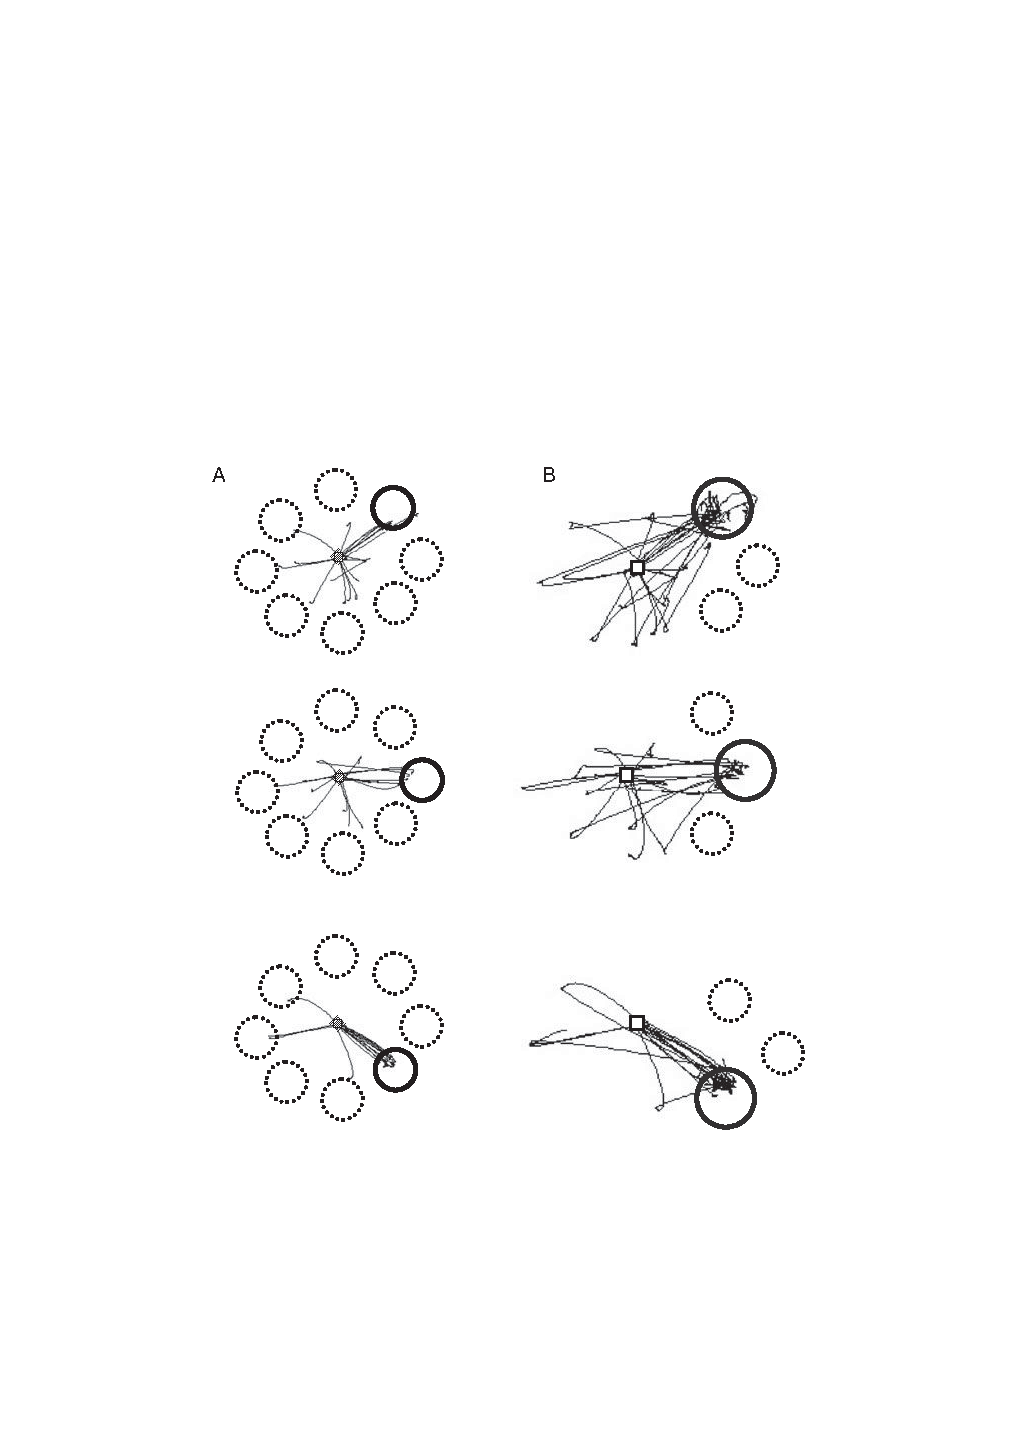
\includegraphics[width=0.7\linewidth]{chap5/Fig_5_8}
	\caption{在一个明显的错误后的纠正性扫视。
		(A)在中外侧前额叶皮层失活后,猴子对错误的目标进行了一些扫视。
		对于图的顶部部分,正确的目标是右上方的位置,对于中间部分,正确的位置,对于底部部分,正确的位置是右下方的位置。
		(B)对一次不正确扫视的直接后果的检查表明,猴子在那次试验中对适当的目标进行了矫正扫视\cite{tsujimoto2012prefrontal}。}
	\label{fig:fig_5_8}
\end{figure}


辻本和波斯特尔还分析了坦率错误的模式,发现猴子经常选择在前一次试验中合适的目标并获得奖励。
因此,很明显,猴子在回溯性空间工作记忆方面并没有简单的损伤。
相反,正如我们在下一章中提出的那样,有前额叶皮层损伤的猴子在区分之前的目标和当前的目标方面有缺陷。


因此,干扰延迟期活动的证据并不支持损伤导致回溯性感觉记忆丧失的观点。
相反,它表明病变干扰了对未标记位置的扫视的准确性,以及区分以前目标和当前目标的能力。
尾侧前额叶受损的猴子似乎保留了正确目标的知识,但很难将这种知识转化为准确的扫视。



\subsection{消除延迟期}

延迟期线索的缺乏导致了延迟期活动反映线索记忆的假设:回顾性空间记忆。
如果是这样,并且如果回溯性空间记忆是尾侧前额叶皮层的关键功能,那么我们可能会认为在没有延迟期的任务中活动减弱。
更重要的是,尾侧前额叶皮层的损伤不应该导致对缺乏记忆要求的任务的损害。
实验结果与这两种观点都不相符。


戈尔德\cite{gold2007neural}向猴子展示了一个由移动的圆点组成的线索。
这些点的净运动,向左或向右,指示扫视一个红色或绿色的目标,而不管目标出现在哪里。
没有延迟期;猴子一旦确定了线索移动的净方向,就会做出选择。


正如我们在第~\ref{chap:chap3}~章中介绍的累加器-跑道模型所解释的那样,戈尔德发现额叶视区中的活动在提示开始和扫视时间之间逐渐增加。
他们表明,这种活动编码了目标刺激的颜色,红色或绿色。
因此,额叶视区在缺乏延迟期或空间记忆需求的任务中具有与任务相关的活动,并且它似乎与包含延迟期的任务一样健壮。


然而,有人可能会说,“记忆”细胞只是在这些任务中变得不活跃,而其他类型的细胞变得更加突出。
因此,一个更有力的预测是,只有在任务包含延迟期时,病变才会造成损伤。
但Keller等人\cite{keller2008effect}提出的证据表明,这一预测并不成立。
他们教猴子一项有条件的视觉运动任务,在这项任务中,动物必须根据中心注视点的颜色,将扫视指向不同的位置。
Keller等人随后单方面或双边地使额叶视区失效。
失活导致错误增加,这些错误不仅包括不准确的扫视,还包括明显的错误。
双侧病变造成的影响大约是单侧病变的两倍。
在这里,这项任务不涉及对回顾性空间记忆的要求,但病变产生了损害。
然而,这些任务确实需要对目标进行前瞻性编码和关注。


到目前为止所描述的任务包括扫视。
但是,关于伸展运动的实验也得出了同样的结论。
劳勒\cite{lawler1987role}教猴子在看到黑色线索后向左伸手,在看到白色线索后向右伸手。
然后,他们在前额叶末梢皮层做了双侧损伤,这造成了严重的损伤。
Petrides\cite{petrides1985deficits}使用视觉提示告诉猴子是打开一个亮着的盒子还是不亮的盒子。
同样,在尾部前额叶皮层有病变的猴子表现出损伤。
这两个实验都没有涉及需要内存的延迟期。


在所有这些任务中,提示都指定了试验的目标,该目标可以是一个地点\cite{keller2008effect}或一个物体\cite{petrides1985deficits}。
目标可以是扫视\cite{keller2008effect}或伸手运动\cite{lawler1987role}的目标。


劳勒和考威\cite{lawler1987role}认为,在尾侧前额叶皮层损伤后,动物“忽视”了部分视觉空间,这意味着它们无法将注意力导向这些地方。
但类似的病变只是增加了寻找外周靶点所需的时间,而不是导致搜索失败\cite{wardak2004deficit}。
因此,我们认为,患有尾侧前额叶皮层病变的猴子可以检测到外周目标,只是比正常情况稍慢一些。
他们的核心缺陷是难以将注意力引导到作为目标的地点和物体上。



\subsection{总结}

本节回顾了来自细胞记录和损伤研究的证据,这些证据已被用于支持前额叶皮层的空间工作记忆理论\cite{goldman1996prefrontal}。
在此,我们对尾侧前额叶皮层(第8区)和后外侧前额叶皮层(第9/46区)否决了这一结论,理由如下:


\begin{enumerate}
	\item 大多数延迟期活动反映了对潜在目标的隐性关注,而不是在记忆中维持感官线索。
	\item 尾侧或后外侧前额叶皮层的损伤很少会造成明显的错误,即猴子会扫视到错误的位置,而不是提示的位置。相反,这些病变主要导致不准确的扫视,比任何其他潜在目标更接近正确的位置。当明显的错误确实发生时,受损的猴子会立即纠正错误,从而表明它们记住了提示的位置。
	\item 这些区域为缺少延迟期的任务编码目标。
	\item 受损的猴子在缺乏延迟期的任务上有缺陷,因此这些区域的功能不依赖于弥合时间差距。
\end{enumerate}
因此,有证据表明,尾侧和后外侧前额叶皮层的功能是寻找和关注目标,而不是工作记忆。
我们在第~\ref{chap:chap6}~章讨论了背侧前额叶皮层,讨论了拒绝工作记忆理论的其他理由。
在第~\ref{chap:chap10}~章中,我们将讨论前额叶皮层作为一个整体的工作记忆理论。



\section{基于学习的注意力}

在前一节讨论的实验中,猴子必须通过使用奖励反馈来影响其在目标中的未来选择,从而学习应该关注哪个目标。
任务的这一特点并不总是得到应有的考虑。
尾侧前额叶皮层功能的一个重要方面涉及目标导向和刺激驱动注意之间的区别。


\subsection{目标导向和刺激驱动的注意力}

目标导向注意和刺激驱动注意之间的区别与学习有关。
在本书中,我们所说的目标是指作为行动目标的物体和地点。
刺激驱动的注意力取决于目标的显著性,例如,它的亮度或突然发生,这吸引了注意力。
这种自下而上的注意力依赖于先天机制,而不是学习。
在以目标为导向的注意中,实验对象必须知道要注意哪些刺激,无论是在猴子身上通过奖励反馈,还是在人类身上通过指令或反馈。


值得注意的是,刺激驱动注意和目标导向注意之间的区别并不对应于弹出式搜索和连接式搜索之间的区别。
在这两种情况下,猴子通过反馈学习目标,或者人通过指令或反馈学习目标。
这两种搜索的不同之处在于,在弹出式搜索中,目标从一组相同的干扰物中脱颖而出,而在联合搜索中,目标与干扰物具有相同的特征,但不同之处在于这些特征的特定组合。
干扰物不需要彼此完全相同。
这两种类型的搜索都需要学习,因此额叶视区的失活会损害这两种搜索的性能\cite{wardak2004deficit}。
此外,当Wardak等人\cite{wardak2010searching}在猴子执行弹出式搜索任务时进行了成像实验,主要的激活发生在尾侧前额叶皮层,包括额叶视区,只有少量的激活在后顶叶皮层。


目标导向的注意力涉及到前额叶皮层,因为它比其他区域更直接地接收有关结果的某些信息。
具体来说,眶额皮层可以提供特定条件和“共同货币”条件下潜在目标的估值。
这些信息可以从眶额皮层传递到与尾侧前额叶皮层相连的其他前额叶区域。
眶额皮层和尾侧前额叶皮层之间的相互作用导致对有价值物体的搜索和关注。



\subsection{增强效果}

当尾侧前额叶皮层将注意力导向一个目标时,一个结果被称为增强效应;
与无人看管的地方相比,在有人看管的地方,细胞对刺激的反应更大。
显性注意和隐性注意都会引起这种效应。


Goldberg\cite{goldberg1972activity}发现了对上丘神经元的增强作用。
这些神经元中有许多对扫视目标表现出增强的活动。
在Goldberg\cite{goldberg1981behavioral}的后续研究中,后顶叶皮层的细胞不仅在扫视(显性注意)之前表现出增强,而且在隐性注意期间也表现出增强。
同样,成像显示参与刺激的激活增强\cite{corbetta2000voluntary},激活增强发生在与参与位置相对应的视网膜位置图区域\cite{brefczynski1999physiological}。


在对额叶视区细胞活动的早期研究中,Goldberg\cite{goldberg1985cerebral}发现对扫视目标(显性注意)有增强效应,但对隐性注意没有。
然而,在后来的一项研究中,Kodaka等人\cite{kodaka1997neuronal}报告说,在一项注意力任务中,当外周刺激变暗时,要求猴子释放一个杠杆,许多细胞显示出视觉反应的增强。
因此,就像在后顶叶皮层一样,额叶视区中的细胞对公开和秘密参与的位置都表现出增强的感觉反应。


Hasegawa等人\cite{hasegawa2000search}记录了8Ad区域,并在一系列干扰物中展示了一个类似物体的目标。
在目标出现的135毫秒内,如果目标出现在细胞的接受野中,这些尾部前额叶皮层细胞的反应就会增强。
如果目标出现在细胞的感受野之外,或者目标以外的刺激出现在感受野,则不会发生增强。
这一发现与尾侧前额叶皮层有助于或反映对学习目标的搜索这一观点一致。



\subsection{自上而下的影响}

鉴于增强效应既发生在前额叶皮层,也发生在更尾部的区域,如后顶叶皮层,我们需要知道是什么驱动了增强。
单从增强效果来看,我们无法区分因果关系。
我们不能简单地假设细胞的反应更多是因为自上而下的注意力的影响。
尽管如此,累加器-跑道网络的特性表明了这种机制是如何工作的(第~\ref{chap:chap3}~章)。
如果前额叶皮层网络代表了未来行动的目标,那么它可能会导致皮层其他地方对该目标的感觉表征更快地达到阈值。
结果是基于学习目标的自上而下的有偏见的竞争\cite{desimone1995neural}。
结果就是“寻找”或保持对目标的注意力。


自上而下的偏差可以解释增强如何发生在低阶区域。
我们已经提到,Armstrong\cite{armstrong2007rapid}将皮质内微刺激应用于额叶视区,并表明它增强了视觉区V4细胞的反应。
它是为视觉空间的一个特定部分做的。
这一发现表明,当猴子注意到空间的这一部分时,额叶视区对V4施加了自上而下的偏向,有利于该位置的表示。


第~\ref{chap:chap3}~章阐述了前额叶皮层可以使低阶行为控制系统之间的竞争产生偏见的想法,Desimone\cite{desimone1995neural}提出了一个对低阶视觉区域自上而下影响的偏见竞争模型。


Desimone和Duncan并没有提供证据证明自上而下的效应起源于前额叶皮层,而不是其他区域。
然而,我们知道,尾侧前额叶皮层的细胞根据当前任务的性质表现出不同的活动。
当线索的位置与行动选择的相关性很小时,只有少数细胞对该位置进行编码\cite{chen2001neuronal}。
当线索的颜色和形状具有高度相关性时,大量的尾端前额叶细胞开始编码这些特征\cite{bichot1996visual}。


相应的变化发生在感觉区域。
当任务要求猴子注意运动时,MT和MST区域的神经元对刺激的特征表现出增强的反应\cite{treue1996attentional}。
当任务要求猴子注意方向时,V4区域的细胞对该特征的反应增强\cite{mcadams1999effects}。


然而,增强效果取决于这样一个事实:
猴子已经学会了哪个维度、动作或形状与任务相关。
动物只有在关注相关维度时才会得到有益的反馈。


尾侧前额叶皮层与吻侧前额叶皮层有广泛的联系,前额叶皮层许多部分的细胞活动反映了当前相关的刺激维度。
例如,Lauwereyns等\cite{lauwereyns2001responses}教猴子一个不去不去的任务,其中相关刺激维度在颜色和运动之间交替。
他们发现,44\%的细胞更喜欢与颜色相关的条件,24\%的细胞更喜欢与运动相关的条件。
前者多位于腹侧前额叶皮层,后者多位于背侧前额叶皮层。
这两个区域的吻侧细胞往往比尾侧前额叶皮层的细胞更常反映相关维度,后者的细胞通常编码适当的反应:去或不去。


Lauwereyns等人将这些位于尾侧的神经元称为“整合细胞”,并认为它们将前额叶皮层的部分输出提供给其他皮层区域。
因此,颗粒状前额叶皮层的吻侧部分会影响尾侧前额叶皮层,从而影响皮层其他部分的感觉信息处理。
他们也可以直接这么做。


如果这种增强是自上而下作用的结果,那么就有可能表明这种增强在前额叶皮层比尾侧感觉区发生得更早。
因此,Zhou\cite{zhou2011feature}在猴子执行视觉搜索任务时,同时从额叶视区和V4区域记录。
当猴子注意到刺激的特定特征时,两个区域都出现了增强的感觉反应,但这些影响的潜伏期表明,额叶视区对V4提供了自上而下的偏向。
由此可见,尾侧前额叶皮层可以调节感觉皮层对刺激特征的加工。


自上而下的注意机制可能涉及两个区域慢波振荡的同步发展。就像通过成像实验测量的信号一样(第~\ref{chap:chap1}~章),电位的缓慢变化可能反映的是突触活动,而不是神经元放电率。
在周和德西蒙的实验中,格雷戈里欧等人\cite{gregoriou2009high}记录了额叶视区和V4,当猴子在细胞的接受野中接受刺激时,他们这样做。
他们观察到这两个区域振荡之间耦合的发展,而额叶视区似乎启动了这种耦合。
同步最显著地发生在伽马带,这被认为是皮层区域之间相互作用的一般机制\cite{womelsdorf2007modulation}。


前额叶皮层的增强比视觉区域更早,这一发现并不能证明前额叶皮层会导致这些区域的增强。
因此,Rossi等人\cite{rossi2009prefrontal}研究了前额叶病变的影响。
他们教猴子辨别铁栅栏上铁条的方向。
中央线索的颜色告诉猴子在有相同颜色的光栅中判断方向。
猴子看到了三个栅格,只有一个有相关的颜色,它可以在不同的试验中改变,也可以在一系列试验中保持不变。
背侧前额叶皮层和腹侧前额叶皮层的单侧病变,加上胼胝体的横断,使得Rossi等人能够比较受损半球和完整半球处理刺激时的表现。
对于受损的半球,猴子表现出严重升高的辨别方向的阈值,相关颜色的频繁变化加剧了这种缺陷。


Rossi等人并没有证明前额叶损伤消除了视觉区域的增强效果,但一些皮层刺激实验提供了证据,证明它可能会。
Morishima等人\cite{morishima2009task}在人类受试者的额叶视区上使用单脉冲经颅磁刺激(TMS)。
他们的实验对象看到了由移动的点组成的脸,并必须对点的运动或脸的性别做出判断。
因此,他们要么注意动作,要么注意面孔。
Morishima等人在刺激额叶视区时,用脑电图记录了MT区域和颞皮质梭状面区域的激活。
当被试准备对运动进行判断时,刺激影响MT区激活,而当被试准备对性别进行判断时,刺激影响梭状回面部区的激活。
因此,刺激部分颗粒状前额叶皮层后视区产生了自上而下的对相关刺激维度的偏向。



\section{总结}

\subsection{尾侧前额叶皮层是如何发挥作用的}

本章展示了尾侧前额叶皮层的连接如何解释它对整个前额叶皮层的贡献。
其中三个联系似乎是最重要的:

\begin{enumerate}
	\item 通过12区和46区,与眶额眶皮层的连接间接地为尾侧前额叶皮层提供了所观看项目的学习和更新价值\cite{barbas1989architecture}。
	\item 通过与背侧和腹侧视觉流的连接,尾侧前额叶皮层搜索并引导注意力到有价值的地方和物体上。
	通过与背侧和腹侧视觉流的连接,尾侧前额叶皮层搜索并引导注意力到有价值的地方和物体。
	这些联系包括对顶叶和颞叶区域的投射,这被认为是导致对地点和物体的感觉反应增强的原因,从而在相互竞争的感觉表征中提供了一种自上而下的偏见。
	\item 通过上丘和基底神经节直接或间接地投射到动眼核,使额叶视区通过眼球运动来引导显性注意力。
\end{enumerate}

这些连接使末梢前额叶皮层能够在混乱的环境中寻找有价值的目标,并将注意力引向这些目标。
它专门针对学习目标——目标导向的注意力——而不是反身性或刺激驱动的注意力。



\subsection{提议}

现在,我们可以用简单而详细的形式提出尾侧前额叶皮层的特定功能:

\begin{enumerate}
	\item 简而言之:尾侧前额叶皮层主要基于视觉,寻找并引导注意力朝向有价值的目标。
	\item 扩展:尾侧前额叶皮层,以及后外侧前额叶皮层,主要基于视觉,根据当前生物需求进行评估,搜索并将注意力导向学习价值的目标。
	它通过隐蔽的注意力或公开的注意力(眼球运动)来做到这一点。
\end{enumerate}



\subsection{为什么其他区域不能做尾侧前额叶皮层所做的事情}

由于它的连接,只有尾侧前额叶皮层可以执行这些功能。
如第~\ref{chap:chap4}~章所示,眶额皮层皮层首先接收到关于食物的视觉、嗅觉、味觉和“口感”的详细信息。
通过与眶额皮层的间接连接,尾侧前额叶皮层可以根据当前的生物学需求接收关于特定目标的可取性的信息。


另一方面,后顶叶皮层无法接收到太多关于特定食物或液体的信息。
它几乎没有(如果有的话)传递特定结果的输入,无论是来自眶额皮层还是来自任何其他皮层区域。
此外,它与杏仁核的联系很少,如果有的话。
颞叶皮层确实接受杏仁核的输入,但它不能像前额叶皮层那样轻易地将这些信号与结果的嗅觉、味觉和内脏特征结合起来。
尾侧前额叶皮层和后顶叶皮层都在注意力中起作用。
但正如我们所强调的,尾侧前额叶皮层负责关注猴子已经学会的有价值的目标,这可能是因为它而不是后顶叶皮层接收有关特定结果的前额叶中介信息。



\subsection{对觅食选择的贡献}

在实验室里,灵长类动物经常以彩色形状或光点的形式去触摸或观察目标。
在它们的自然环境中,它们的目标包括食物、食物的标志和有学习价值的地方。
正如第~\ref{chap:chap2}~章所解释的那样,在早期灵长类动物中进化出的前额叶皮层有两个新的颗粒区域:尾侧前额叶皮层和眶额皮层的颗粒部分。


我们认为,这两个颗粒区域在早期灵长类动物中共同起作用,就像在现代灵长类动物中继续起作用一样。
但要了解它们是如何影响早期灵长类动物的觅食选择的,我们需要了解这些已经灭绝的“视觉动物”是如何看待世界的。


通过我们自己的眼睛去看其他动物的视觉,这是我们人类的一种自负。
但是早期的灵长类动物没有像我们这样的眼睛,很大程度上是因为它们缺少一个后来进化出来的中央凹(第~\ref{chap:chap2}~章)。
根据定义,显性注意力依赖于中央凹,所以当早期的灵长类动物关注和搜索物体时,它们使用隐性注意力来做到这一点。
我们提出,早期灵长类动物的眶额皮层根据当前需求提供了可见物体的学习价值(第~\ref{chap:chap4}~章)。
当与尾侧前额叶皮层提供的搜索和注意力功能相结合时,早期灵长类动物可以在物体和地点中进行选择,在杂乱的环境中找到它们,并(秘密地)关注它们。


在灵长类动物进化的后期,出现了中央凹和三色视觉,并出现了新的前额叶区域(第~\ref{chap:chap2}~章)。
接下来的两章,分别在背侧前额叶皮层和腹侧前额叶皮层,探索这些区域给类人猿灵长类动物带来了什么优势。



\chapter{背侧前额叶皮层:基于最近事件生成目标} \label{chap:chap6}

背侧前额叶皮层有助于根据顺序、时间和空间环境生成目标,它的连接解释了为什么只有它才能做到这一点。
背侧前额叶皮层,包括中外侧前额叶皮层(46区),通过与后顶叶皮层、前运动皮层和前额叶皮层的其他部分连接来发挥作用。
顶叶连接提供了许多用于生成目标的空间和时间背景。
与运动前区域的联系导致这些目标的实现,通常是通过手的运动。
与\textit{眶额前额叶皮层}的连接使背侧前额叶皮层能够根据\textit{单个事件}预测\textit{目标选择的具体结果}。
背侧前额叶皮层位于背侧视觉流的末端,因此它可以规划目标序列,它可以具体或抽象地指定这些目标。
在产生目标后,背侧前额叶皮层可以前瞻性地编码它们,直到行动的时候到来。
鉴于背侧前额叶皮层在类人猿灵长类动物中进化(第~\ref{chap:chap2} 章),我们认为它在使用最近视觉事件的顺序、时间和位置来指导觅食选择和生成效率优化的目标序列方面具有优势。



\section{介绍}

第~\ref{chap:chap2}~章解释了灵长类动物的前额叶皮层在类人猿中随着新区域的出现而扩展。
第~\ref{chap:chap3}~章涉及了其中的一些,例如额极皮层(10区),但在本章和下一章,它们是主要主题。
由于类人猿依赖于白天漫长的觅食旅行,它们需要消耗大量的能量,并面临着很高的捕食风险。
这种生活方式非常重视正确的觅食选择。
在影响这种选择的因素中,视觉事件的位置、时间和顺序是突出的,因为类人猿利用了它们在中央凹和色彩视觉方面的进步。
正如第~\ref{chap:chap2}~章所解释的,这些进步包括中央凹提供的精致的视觉敏锐度和三色视觉提供的增强的辨别能力。


这一章解释了觅食的选择部分取决于当前的环境,
这是由选择时可用的刺激以及最近视觉事件的记忆所指定的。
为了理解我们的意思,考虑一个简单的实验室任务:延迟匹配样本。
猴子把一个刺激看作一个样本,然后看到一个或多个刺激需要选择。
这种选择不仅取决于选择时的刺激,还取决于基于样本刺激的记忆。
这两个因素共同构成了当前选择目标的背景。


由于记忆对当前情境起作用,这类实验的被试面临一个问题:最近发生了几件事,并选择了几个目标。
本章的大部分内容探讨了背侧前额叶皮层如何帮助类人猿灵长类动物解决这个问题。
许多文献都依赖于一个任务和一个区域:延迟反应任务,它依赖于中外侧前额叶皮层(46区)。
因此,我们将讨论的重点放在第~\ref{chap:chap1}~章和第~\ref{chap:chap5}~章也提到的这个任务上。
我们认为,因为受试者在这个任务中经历了一系列的视觉事件,并实现了一系列的目标,他们需要挑选出决定当前目标的事件。
然后,我们回顾一系列其他任务,这些任务也要求主体在当前环境的基础上生成目标。



\section{区域}

在猕猴中,中外侧前额叶皮层位于主枕沟的嘴侧三分之二(图~\ref{fig:6_1})。
然而,它也延伸到这个沟的背侧和腹侧的凸面皮层。
中外侧前额叶皮层(46区)有很多名字,有些很明确,有些则不太明确。


\begin{figure}
	\centering
	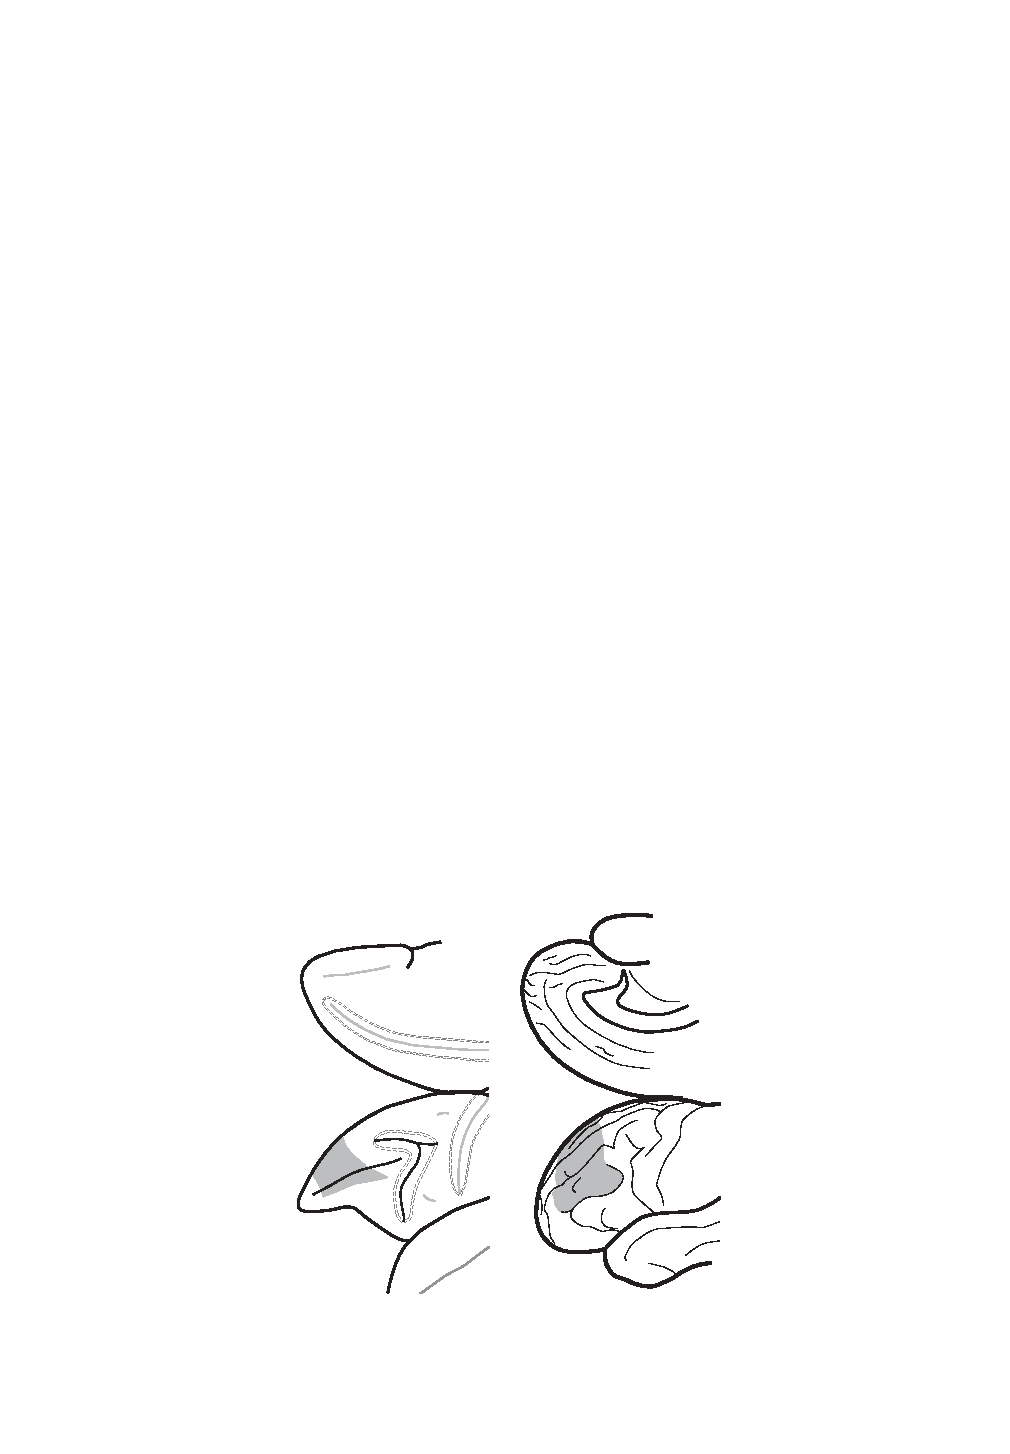
\includegraphics[width=0.7\linewidth]{chap6/6_1}
	\caption{猕猴(左)和人类(右)的背侧前额叶皮层。
		格式如图~\ref{fig:1_2}~所示。}
	\label{fig:6_1}
\end{figure}


\textit{沃克}将沿主沟整个长度的皮层称为46区\cite{walker1940cytoarchitectural},但最近\textit{佩特里迪斯}将9/46区区分为该沟的尾端周围(见图~\ref{fig:1_2})\cite{petrides1999dorsolateral}。
为了避免对46这个术语的不同用法的混淆,我们称沃克46区嘴侧三分之二为中外侧前额叶皮层,尾侧三分之一为后外侧前额叶皮层。
在人类中,这些分区位于额上回和额下沟之间。


尽管出现了这些新术语,但混淆的空间仍然很大。
术语背侧前额叶皮层最初是指猴子的整个侧前额叶皮层\cite{pribram1952effects},但后来仅指主沟内和背侧的皮层\cite{mishkin1969re}。
在影像学文献中,指背外侧前额叶皮层已变得很常见,但该术语的使用通常非常松散,很少注意解剖标志。
因此,我们在本书中避免使用这个术语。
表~\ref{tab:1_2}~给出了我们所采用的术语。
我们将背侧前额叶皮层包括主沟两岸的皮层和其背侧的凸面皮层(区域9),但不包括区域9的内侧部分。
当然,这些划分并不是最终的结果,但它们在一定程度上反映了联系。



\section{连接}

图~\ref{fig:6_2}~展示了\textit{背侧前额叶皮层}的一些皮层连接。
正如第~\ref{chap:chap1}~章所解释的,这些连接构成了解剖指纹。
\par


1.中外侧前额叶皮层(46区)与后顶叶皮层,特别是尾顶叶区有很强的联系\cite{petrides1984projections}。
正如前一章所提到的,后顶叶皮层的许多神经元编码视觉空间信息。
然而,顶叶细胞也编码时间间隔\cite{leon2003representation},当人类受试者对近期事件做出判断时,左侧顶叶内沟会出现激活\cite{dudukovic2007goal}。
\par


2.中外侧前额叶皮层连同外侧9区,与位于上颞沟上排的多感觉\textit{颞顶枕区}(也称为\textit{上颞多感觉区})相连\cite{seltzer1996overlapping}。
该区域的细胞对体感、听觉和视觉刺激有反应\cite{bruce1981visual}。
\par


3.中外侧前额叶皮层也接受来自周围皮层的输入\cite{petrides1999dorsolateral},其功能是识别物体\cite{murray2007orbitofrontal}。
这种联系表明,中外侧前额叶皮层接收到有关物体的直接输入,而不仅仅是腹侧前额叶皮层的间接输入(第~\ref{chap:chap5}~章和第~\ref{chap:chap8}~章)。
\par


4.中外侧前额叶皮层接收来自\textit{次级躯体感觉皮层}\cite{petrides2002comparative}和下顶叶嘴侧PFG区\cite{rozzi2006cortical}的输入。
这些区域的细胞对体感刺激有反应\cite{hyva1981regional},中外侧前额叶皮层的细胞也是如此\cite{tanila1993regional}。
这一特征将中外侧前额叶皮层与尾侧和后外侧前额叶皮层区分开来,后者的细胞主要具有视觉和注意力特性(第~\ref{chap:chap5}~章)。
\par


5.中外侧前额叶皮层连接背侧和腹侧前运动皮层\cite{wang2002spatial},以及\textit{前辅助运动区}\cite{wang2005prefrontal}和位于\textit{扣带沟}的嘴侧\textit{扣带运动区}\cite{dum1993cingulate}。
这些投影主要涉及代表手和手臂的运动前区域,而不是脚和腿。
前肢表征的专门化表现在背侧前前皮层的嘴侧部分\cite{tachibana2004input}、腹侧前运动皮层\cite{he1993topographic}、\textit{前辅助运动区}\cite{luppino1991multiple}和\textit{扣带运动区}\cite{he1995topographic}。
因此,相对于运动的移动,中外侧前额叶皮层在伸手、操作和进食运动中具有优先的作用(第~\ref{chap:chap2}~章)。
\par


6.中外侧前额叶皮层与前扣带皮层有很强的联系\cite{petrides1999dorsolateral}。
第~\ref{chap:chap3}~章解释了前扣带皮层在动作评估和基于这些评估动作之间的切换中发挥作用\cite{walton2007adaptive}。
\par


7.中外侧前额叶皮层与\textit{压后皮层}相连\cite{morris1999fiber}。
反过来,从\textit{压后皮层}投射到海马旁回和下丘前\cite{kobayashi2007macaque}。
我们认为,这些联系可能在有关事件的记忆检索中发挥作用,而这种检索依赖于时间或空间上下文\cite{vann2009does}。
\par


8.区域9的横向部分连接受到的关注相对较少,部分原因是很少有功能数据引起人们的兴趣。
这部分背侧前额叶皮层与\textit{背侧前运动皮层}的嘴侧部分\cite{petrides1999dorsolateral}和\textit{扣带运动区}\cite{morecraft1993frontal}有联系。
就像第9区域的内侧部分一样,它也与上颞皮层有联系,这可能传达听觉信息\cite{petrides1984projections,saleem2008complementary}。
最后,第9区外侧部分与后顶叶皮层下部(PG区)\cite{cavada1989posterior}和\textit{压后皮层}\cite{kobayashi2003macaque}相连。


\begin{figure}
	\centering
	\includegraphics[width=0.7\linewidth]{chap6/6_2}
	\caption{背侧前额叶皮层的选定连接。
		图~\ref{fig:1_4}~和~\ref{fig:1_5}~给出了沟和区域的名称。
		除非另有说明,一些轴突与背侧前额叶皮层有直接连接的区域被认为是相互的。}
	\label{fig:6_2}
\end{figure}



\subsection{总结}

中外侧前额叶皮层与后顶叶皮层、前运动皮层有很强的联系,并间接与海马系统有联系。
它也与前额叶皮层的其他部分相互连接,如眶额皮层。
其他皮层区域没有这种连接模式。
因此,它很好地整合了由\textit{眶额皮层}、\textit{背侧视觉流}和\textit{海马体}处理的信息,并向\textit{前运动皮层}提供信息。



\section{延迟响应任务}

中外侧前额叶皮层在接收后顶叶皮层的视觉空间信息方面与尾侧前额叶皮层相似。
因此,任何一个区域的损伤都会导致猴子在动眼延迟反应任务和经典版本的延迟反应任务上的表现中断,这并不奇怪。
在这两项任务中,空间线索指导目标选择,猴子必须在可能的空间目标中进行选择。
当然,根据定义,动眼肌延迟反应任务需要对目标进行扫视,而经典的延迟反应任务需要达到目标的运动。
第~\ref{chap:chap5}~章解释了尾侧前额叶皮层和后外侧前额叶皮层的损伤会导致动眼力延迟反应任务的准确性误差,根据它们与背侧视觉流的连接,这是有意义的。
这些损伤不会引起很多明显的错误,当它们发生时,猴子会迅速纠正这些错误\cite{tsujimoto2012prefrontal}。


相反,中外侧前额叶皮层(46区)的永久性损伤对经典的延迟反应任务造成毁灭性的损害。
当猴子在手术前学习延迟反应任务时,它们在中外侧前额叶皮层损伤后执行任务的效果并不比偶然水平好\cite{goldman1978prenatal}。
也就是说,受损的猴子犯的错误和正确的选择一样多。
当他们在中外侧前额叶皮层持续受损后第一次尝试学习任务时,即使有短暂的(1秒)延迟期,他们也无法完成任务\cite{battig1960comparison}。
而且它们永远无法恢复,至少在任何人测试过的时间范围内都无法恢复。


一个重要的方法差异可以解释这种差异的部分原因。
在经典的延迟反应任务中,猴子伸手去拿盖在食物井上的盖子。
这意味着在这个版本的任务中,不像动眼肌延迟反应任务,受试者只能犯明显的错误。
如果发生,精度错误将不会被记录。


另一个区别可能也很重要。
猴子可以通过在延迟期间偷偷地关注目标位置来解决动眼肌延迟反应任务。
但是实验者执行经典延迟反应任务的方式使得隐蔽注意力很难集中到目标上。
传统的测试方法包括\textit{威斯康辛通用测验仪}。
在该仪器中,一个不透明的屏幕在延迟期间下降,使猴子在延迟期间无法看到相关位置(图~\ref{fig:6_3})。
在神眼运动版本的任务中,猴子可以在周边视觉中看到目标位置,尽管在扫视时它不再被标记出来。


原则上,执行经典延迟反应任务的猴子仍然可以准确地注意到\textit{威斯康辛通用测验仪}的目标一侧,或者以某种方式将姿势定向到那一侧。
然而,降低屏幕往往会导致猴子在测试室内移动。
Passingham\cite{passingham1971behavioural}在延迟期间监测了正常猴子的位置,发现即使它们已经解决了问题,在40\%的试验中,它们也会从房间的一边穿过到另一边。
因此,猕猴不需要通过身体定位来解决延迟反应任务所带来的问题,似乎测试方法很可能排除了使用隐蔽注意力来解决这个问题。
因此,动眼肌延迟反应相对缺乏坦率的错误可能反映了隐蔽地关注目标位置的持续能力,而延迟反应任务的经典版本的严重损害可能是由于破坏了这一策略。


当然,延迟响应任务可以在没有不透明屏幕的情况下呈现。
在延迟期间,食物井可能在受试者够不到的地方。
在这种情况下,猴子似乎更有可能采取某种姿势或注意力的方法来弥合延迟期,或者使用其他策略来做到这一点。
Wilson\cite{wilson1963effect}发现。正常的猴子在延迟期开始时坐在测试室的正确一侧,在延迟期结束时仍保持在该一侧。
然后,当他们有机会这样做时,他们就会到达离目标最近的距离。
在延迟开始时,有前额叶皮层损伤的猴子也坐在正确的一侧,但在延迟结束时,它们到达相反(错误的)目标的次数与到达正确目标的距离较短的次数一样多。
这一发现表明,对于有前额叶损伤的猴子来说,姿势或注意力的延迟期桥接不足以正确地形成延迟反应任务。


目前还不清楚为什么猴子在整个延迟期间不采取保持在\textit{威斯康辛通用测验仪}正确一侧的策略。
这个策略可以解决问题。
也许他们没有意识到,他们在延迟期开始时看到的东西表明了他们在延迟期结束时应该达到的目标。
换句话说,受损的猴子可能无法识别延迟间隔之前的视觉事件与它们即将做出的选择有任何关联。
正常的猴子确实认识到这种关系,并且不需要采取姿势定向策略或注意力策略来执行任务。


在后面的部分中,我们提出了这样的想法,即为了解决延迟响应任务所带来的问题,猴子需要知道延迟期之前的视觉事件为它们之后选择目标提供了关键。
我们认为,中外侧前额叶皮层受损的猴子要么无法学习这一规则,要么无法记住和应用它。


\begin{figure}
	\centering
	\includegraphics[width=0.32\linewidth]{chap6/6_3}
	\caption{在\textit{威斯康辛通用测验仪}中延迟响应任务的测试程序。
		(A)实验员在两个食物井(+)中的一个上饵,一只猴子从它的测试笼中观察。这个动作作为视觉提示事件。
		(B)实验者在延迟期间放下一个不透明的屏幕。
		相同的物体可以很好地覆盖食物。
		(C)实验者举起屏幕后,猴子在两个食物井中进行选择,将其中一个物体移开,如果正确(+)则获得奖励,如果错误(-)则得不到奖励\cite{murray1991contributions}。}
	\label{fig:6_3}
\end{figure}



\subsection{延迟期的重要性}

第~\ref{chap:chap5}~章提到,尽管尾侧前额叶皮层病变的猴子在动眼力延迟反应任务上只有轻微的损伤,但它们在没有延迟期的条状视动任务上也有损伤。
相比之下,在中外侧前额叶皮层有损伤的猴子只在包括延迟期的任务中有损伤。


Passingham\cite{passingham1985memory}设计了一个没有延迟的条件视觉运动任务。
显示器中央的两个面板,一个在另一个上面,提供线索。
猴子们知道,如果光出现在顶部的面板上,那么它应该选择一侧的目标;
如果一个光出现在底部面板,那么它应该选择另一边的目标。
所以这个任务包括空间线索和空间目标就像延迟反应任务一样,但不像延迟反应任务它不包括延迟期。
中外侧和后外侧前额叶皮层病变的猴子可以正常学习这项任务。


Stamm\cite{stamm1969electrical}的结果也表明,延迟是产生损伤的关键因素。
在一个试验中,他在不同的时间点灭活了中外侧或后外侧前额叶皮层。
在延迟期的早期,中外侧前额叶皮层(46区)的破坏估计导致延迟反应任务的表现下降到机会水平。
刺激后外侧皮层效果较小。
这一发现与Butters\cite{butters1969retention}的一项研究结果一致,他们在该研究中表明,主沟中央三分之一的病变导致延迟交替任务的严重损害,而后三分之一的病变的影响要小得多。


综合来看,这些结果支持两个结论。
首先,延迟响应任务的损害确实是由于延迟期的强加造成的。
其次,中外侧前额叶皮层在这一任务中起着必要的作用。
在密切相关的延迟交替任务中也是如此。



\subsection{延迟周期活动}

关于延迟反应障碍,最常被引用的说法是猴子无法记住线索的位置,因此这种缺陷可以被描述为回溯性空间工作记忆的缺陷之一。
人们可以记录下延迟期间的活动,而且乍一看,这种活动似乎是对线索位置的记忆编码,这一事实被解释为支持这一结论的证据。
然而,这种活动发生在前额叶皮层的许多部分,以及其他区域。
第~\ref{chap:chap5}~章解释了延迟期活动并不总是编码空间记忆。
当研究人员在充分的比较条件下研究细胞活动时,他们可以看到大部分所谓的记忆活动实际上编码了参与的位置。
然而,一些延迟期活动确实编码了记忆的位置,因此,中外侧前额叶皮层的延迟期活动仍然有可能介导回溯性工作记忆。


Kojima和Goldman-Rakic(1984)从中外侧前额叶皮层(46区)进行记录,试图验证空间工作记忆理论。
他们使用了两种条件。
在一种情况下,线索在延迟期间消失,而在另一种情况下,线索在整个试验过程中仍然可见。
在延迟期间编码位置的62个细胞中,当刺激仍然可见时,44个细胞表现出相同或更大的延迟期活动。
当刺激消失时,只有12个细胞更活跃。
Tsujimoto\cite{tsujimoto2004properties}在类似条件下使用了动眼肌延迟反应任务,并证实了这一结果模式。


对这一发现最有可能的解释有四种:
\par


1.即使线索仍然可见,也没有什么能阻止猴子“记住”它的位置。
因此,在这两种情况下,它们可能会“记住”提示的位置。
\par


2.在这两种情况下,猴子可能会视觉注意住目标。
Kojima和Goldman-Rakic(1984)没有记录眼睛的位置,所以我们不能排除他们的结果是由于明显的注意力。
\par


3.在这两种情况下,猴子可能会偷偷地关注目标。
\par


4.在这两种情况下,猴子脑内可能会对空间目标的位置进行编码。
这种表述可能包括一个计划好的行动,也可能独立于实现目标所需的行动而指定目标。


在这四种解释中,只有第一种与Kojima和Goldman-Rakic(1984)的解释是一致的。
他们得出的结论是,延迟期的活动反映了线索在回顾记忆中的位置,这与空间工作记忆理论一致。
然而,猴子似乎不太可能“记住”它们能看到的刺激。
第二种说法,就公开关注而言,可以解释island和gleman-lajiki的结果,但不能解benziko的结果。
在后一项研究中,猴子必须在整个延迟期间固定在一个中心位置。
第三种解释,即隐性注意,也可以解释两项研究的结果,但它与回溯性工作记忆方面的解释不相容。


这就剩下了第四种解释,它将延迟期活动解释为反映了空间目标的位置,这是Fuster\cite{fuster1973unit}首次提出的。
换句话说,这表明延迟期反映的是前瞻性记忆,而不是回顾性记忆。
猴子每天进行多次试验,这意味着先前试验的线索和目标位置在记忆中相互干扰。
在任何特定的试验中,只要看到线索,猴子就能通过编码目标位置来克服这种干扰。


第~\ref{chap:chap5}~章回顾了一些似乎反对目标的前瞻性编码的证据。
大多数细胞编码反眼跳任务中的线索位置,只有少数编码目标位置。
在另一项研究中,细胞对提示位置进行编码,即使这些位置不是未来的目标。
然而,这些研究都没有明确地关注中外侧前额叶皮层的细胞,而不是后外侧或尾侧前额叶皮层。


在本章稍后将详细介绍的一项研究中,Genovesio等人\cite{genovesio2006representation}确实研究了中外侧前额叶皮层中的细胞,以及其他神经元种群,他们的实验设计允许他们区分位置的回顾性编码和前瞻性编码。
他们发现,中外侧前额叶皮层的细胞尽可能快地编码当前的目标位置,并且回溯编码在这个时候消失。
我们还在后面的一节中提供数据,表明这种预期的活跃度可以防止内存干扰\cite{sakai2002active}。



\subsection{总结}

中外侧前额叶皮层损伤的猴子在机会水平上执行延迟反应任务,并且它们没有恢复。
在延迟期间的破坏性电刺激会导致损伤,在没有延迟期的任务中,猴子表现正常。延迟期活动发生在中外侧前额叶皮层,它编码一个位置。
这种活动已经被解释为回顾性空间记忆,但证据表明,这种活动也编码了当前目标的位置(预期编码)和参与的位置。



\section{干扰的作用}

在延迟反应和延迟交替任务上,每天都有一系列的试验展开,这对记忆造成了严重的干扰。
在延迟反应任务中,随着试验次数的增加,猴子会从两个或多个位置获得线索;
在延迟反应和延迟交替任务中,猴子在一系列试验中选择了相同的地点。



\subsection{干扰效应的证据}

Diamond\cite{diamond1989comparison}的一项实验表明,干扰可能是导致延迟反应障碍的重要因素。
他们在修改后的延迟反应任务中测试了背侧前额叶损伤的猴子,并分析了猴子在两次正确选择同一侧后所犯的错误。
当这次测试的正确位置碰巧与前两次测试的正确位置相匹配时,猴子的正确率为85\%。
当当前试验中的正确位置与前两次试验不匹配时,猴子的表现符合概率水平(50\%正确)。


有人可能会试图解释这一发现,认为猴子坚持不懈。
但是,坚持不懈会导致低于机会的表现,相反,猴子表现在机会水平(50\%正确)。
事实上,受损的猴子在机会水平上的表现表明,它们意识到线索与前两次试验不同。
然而,他们不知道该选择哪个位置,所以他们的选择基于这样一个事实:
两种可能的选择产生的奖励频率与最近几次试验的平均值大致相同。


正常的猴子可以学会根据单一事件做出选择。
在经典的延迟反应任务中,这个事件包括看到一颗花生被放在其中一个食物井里。
在其他版本的延迟响应任务中,相关事件由空间某处闪烁的视觉提示组成。


在第~\ref{chap:chap4}~章中,我们指出,患有眶前额叶损伤的猴子不会坚持,而是根据过去的事件历史(经过多次试验的平均值)来选择对象。
相比之下,完整的猴子可以将结果分配给似乎导致结果的单一、具体的选择。
我们认为中外侧前额叶皮层也有类似的情况。
在延迟响应任务中,在延迟期间之前的可视事件导致基于该单个事件生成适当的目标。
如果没有这种影响,我们的选择将取决于许多先前事件的平均值。


Diamond和Goldman-Rakic使用的延迟反应任务是对Piaget\cite{piaget1955construction}设计的任务的修改,该任务用于评估人类婴儿理解物体持久性的能力。
它被称为“A-not-B”任务。实验者在a位置藏了一个玩具,婴儿拿了出来。
然后他们把玩具藏在位置b。即使婴儿看到这个视觉事件,他们倾向于回到位置A\cite{harris1989object}。


A-not-B任务通常要求婴儿伸手去找他们看不到的目标。
值得注意的是,他们有时甚至可以在透明覆盖物下看到位于B位置的物体时到达A\cite{butterworth1977object}。
因此,婴儿似乎记得他们在最近的过去选择了A位置来获得玩具,所以他们再次这样做,而不是根据最近的视觉事件来选择玩具。
换句话说,他们似乎重复一个最近强化的选择,而不是根据玩具隐藏在B位置的视觉事件做出选择。
当儿童更成熟时,他们很容易学会使用最近的事件,即玩具隐藏在B位置,来选择那个位置作为他们的目标。


以同样的方式来看,延迟响应任务的损害可以说是解决试验间干扰的困难,而不是追溯记忆的失败。
从这个角度来看,试验对试验的干扰是由先前在A-非B任务中选择位置A或先前在延迟响应任务中选择替代位置引起的。


为了支持这一想法,有影像学证据表明,当记忆受到干扰时,中外侧前额叶皮层的作用。
Owen等人\cite{owen1999redefining}给人类受试者两个空间任务。
在其中一个位置中,他们介绍了五个位置,并随后立即测试了这些物品的内存。
另一个任务是n-back任务。
在两背任务中,实验者在一系列位置呈现刺激事件,受试者必须指向两个事件之前出现刺激的位置。
因此,n-back任务类似于延迟响应任务,因为出现了一系列项目,并且主题必须将相关项目与无关项目区分开。
空间刺激的顺序决定了相关的位置。
在第一个任务中,尾部前额叶皮层 (区域8)发生了激活,其顺序无关紧要,但中外侧前额叶皮层未发生激活。
但是,在与顺序相关的n-back任务中,激活也发生在外侧前额叶皮层中。


Gray等人\cite{gray2003neural}直接表明n-back任务涉及干扰。
他们对faces使用了三背任务,并比较了高干扰和低干扰条件。
高干扰条件在所有刺激演示中都使用了相同的面孔。
低干扰条件使用了新颖的面孔两次或四次试验作为干扰因素。
与分散注意力的面孔是新颖的相比,当分散注意力的面孔与目标面孔来自同一组时,受试者的表现要差得多。
在同一项研究中,Gray等人发现,在高干扰条件下表现更好的受试者中,前额叶皮层中部和其他区域的激活更多。



\subsection{间隔试验}

与Gray等人\cite{gray2003neural}的成像研究一样,人们可以通过直接操纵干扰来研究干扰。
例如,每天只能在一次试验中测试一下猴子。
Wilson等人\cite{wilson1963effect}做了该实验,发现即使没有试验到试验的干扰,具有较大前额叶皮层损伤的猴子仍然在偶然水平上执行延迟响应任务。


这个结果有两种可能的解释。
首先,猴子可能没有学会这样一个规则,即他们在延迟期之前观察到的结果决定了他们在延迟后应该选择什么目标。
其次,Wilson等人的病变。
包括腹侧前额叶皮层和眶额皮层。
随后的实验表明具有腹侧和眶前额叶皮层合并病变的猴子\cite{passingham1971behavioural},或单独的眶额皮层病变\cite{meunier1997effects},对延迟反应任务有损伤。
如果,正如第~\ref{chap:chap4}~章所讨论的,眶额皮层学习选择和结果之间的关联,这些关联的丧失可以解释威尔逊等人看到的部分损害。
在这个观点上,仍然可能需要中外侧前额叶皮层来解决从试验到试验的干扰,因为Wilson等人报告的损害可能是由其他因素引起的。
根据这一说法,面对先前试验的干扰,中外侧前额叶皮层对于执行延迟响应任务是必要的。
当没有这种干扰时,如在Wilson等人的实验中,根据预测的结果执行任务时,眶额皮层是必需的。



\subsection{对象的使用}

除了简单地减少干扰,还可以通过在每次试验中使用不同的项目来消除干扰。
类似延迟响应的任务只能涉及有限数量的位置,但是类似的任务可以使用无限数量的对象或图片。
Levy\cite{levy1999association}在每次试验中提出了三个新颖的对象,并给了猴子一个选择一个对象的机会。
随后出现了延迟,延迟之后,猴子不得不选择其他物体之一。


\textit{佩特里迪斯}\cite{petrides1995impairments}将此称为 “自我排序” 任务,因为猴子可以选择选择对象的顺序。
因为我们知道对象是命令对象还是实验者命令对象并不重要,所以我们更喜欢将其称为有序对象任务。
Levy和Goldman-Rakic向猴子传授了这项任务,然后形成了病变,包括中外侧和后外侧前额叶皮层,一起或前额叶皮层的背凸度。
两组中的猴子都正常执行有序的对象任务。


然而\textit{佩特里迪斯}\cite{petrides1995impairments}发现,具有背侧前额叶皮层损伤的猴子在有序的对象任务上显示出严重的损伤 (图~\ref{fig:6_4})。
与其的实验一样,由于相同的原因,无法用坚持不懈的方式来解释此结果。


在后来的研究中,\textit{佩特里迪斯}\cite{petrides2000dissociable}显示,当图片用作刺激材料时,具有中外侧前额叶皮层(区域46)或背凸度(区域9)损伤的猴子也显示出此任务的损伤。
在一组更大的物体(从三到五个不等)的情况下,猴子表现出更大的损伤。


对Levy和Goldman-Rakic的研究与\textit{佩特里迪斯}的研究在关键方面有所不同。
\textit{佩特里迪斯}在试验中重复使用了相同的物品,因此猴子必须根据最近接触过的物体或图片来选择。
在此任务中,\textit{佩特里迪斯}产生了高度的审判间干扰。
相比之下,Levy和Goldman使用了新颖的物体,因此避免了干扰效应。
因此,病变在高干扰条件下引起损伤,但在低干扰条件下不会引起损伤。
这些发现支持两个相关的想法: 从试验到试验的干扰会导致中外侧前额叶皮层病变后的缺陷,而该区域会减轻正常猴子的干扰。


\begin{figure}
	\centering
	\includegraphics[width=0.45\linewidth]{chap6/6_4}
	\caption{来自有序对象任务的结果,也称为自有序任务。
		正常(对照)猴子(白条)和有病的猴子(阴影线条)的正确率。
		填充的圆圈表示每个主题的表现,用垂直线表示范围\cite{petrides1995impairments}。}
	\label{fig:6_4}
\end{figure}



\subsection{总结}

在涉及对象的任务中,每个试验使用不同的项目时,具有中外侧前额叶皮层病变的猴子表现正常; 
但是,当实验者从试验到试验使用相同的刺激集时,病变的猴子的表现接近偶然水平。
当然,在延迟响应和延迟交替任务中,实验者使用从试验到试验的同一组地点,而受损的猴子也具有接近偶然的水平。
因此,未能解决思考间的干扰可能会导致延迟响应和延迟交替任务的损害。


然而,结果没有区分对干扰易感性的三种可能解释:
\par


1.猴子在判断事件的时间顺序时可能会出错。
\par

2.他们可能不知道指导任务执行的规则。
\par

3.他们可能无法通过对目标进行前瞻性编码来补偿干扰。

我们将在接下来的三个部分中依次讨论这些可能性。



\section{时间顺序}

第一种解释表明,具有中外侧前额叶病变的猴子在区分两种刺激事件中的哪一种方面存在障碍,例如最近出现的左提示与右提示。
随着一系列试验的展开,它们按时间顺序发生,只有一个是最近的。
可以通过要求猴子根据发生的顺序在两个项目之间进行选择来测试一下第一个解释。
在每次试验中使用不同的物品消除了干扰影响。


\textit{佩特里迪斯}\cite{petrides1991functional}做了这个实验,要求猴子选择更早而不是更晚出现的物体。
他以给定的顺序提出了四个对象,后来又同时提出了两个对象作为选择。
他在每次审判中都使用了新颖的物品。
受害的猴子可以在序列中的第一项与任何替代项之间正确选择,或者在最后一项与任何替代项之间正确选择。
但是这些选择并没有告诉我们什么,因为选择第一个刺激总是会带来回报,就像避免系列中的最后一个刺激一样。


在关键测试一下中,猴子必须在系列中间发生的项目之间进行选择。
在四项系列中,第二项和第三项占据了这个中间地带。
\textit{佩特里迪斯}发现,中外侧前额叶皮层的背侧部分(区域46)的损伤在基于顺序区分项目方面造成了损害,特别是对于第二和第三项目(图~\ref{fig:6_5})。
他在五项系列中获得了类似的结果。


\begin{figure}
	\centering
	\includegraphics[width=0.7\linewidth]{chap6/6_5}
	\caption{串行时序任务的结果。
		在图~\ref{fig:6_4}~的格式中,除了纵坐标绘制了掌握问题的天数。
		根据它们在一系列项目中的排名,每对条将正常(对照)猴子(白条)和损伤猴子(阴影条)进行比较,以在两个项目之间进行选择 [1... 4]。
		垂直线虚线将涉及端点项(项目1或4)的选项与不包括端点的选项分开。
		对于后者,具有中外侧前额叶皮层病变的猴子在测试天数(失败) 的限制内未掌握问题。
		重新绘制自\textit{佩特里迪斯}背外侧额叶皮层内的功能专门化,用于序列顺序记忆\cite{petrides1991functional}。}
	\label{fig:6_5}
\end{figure}


猴子可以学习这项任务,但只有困难。
人类受试者发现使用一系列新颖的图片很容易学习任务。
Milner等人\cite{milner1985frontal}报道,额叶切除术的患者在选择最近发生的图片方面表现不佳。
他们不太可能失败,因为他们不知道规则,因为在每次试验中,实验者都要求他们选择最近的照片。


当然,这种损害可能是由这些大病变的任何部分引起的。
因此,Amiez\cite{amiez2007selective}对人们进行了成像实验,因为他们判断两个刺激中的哪一个在序列中较早出现。
激活发生在前额叶中外侧皮层。


中外侧前额叶皮层中单细胞编码顺序的发现支持了病变和激活研究。
Ninokura等人\cite{ninokura2003representation}依次呈现了三种彩色图案,猴子学会了按此顺序触摸它们。
在中外侧前额叶皮层中,43\% 具有延迟周期活性的细胞编码了出现图片的序列。
Funahashi等人\cite{funahashi1997delay}发现了空间刺激的相似结果。
他们的猴子必须按照它们出现的顺序选择两个目标,以及表现出延迟期活性的中外侧前额叶皮层细胞,62\% 编码的刺激顺序。


Warden\cite{warden2007representation}的一项研究提出了一种可能的顺序编码机制。
他们记录在中外侧前额叶皮层,而猴子执行一项任务,他们必须判断最近发生的两张照片中的哪一张。
第二张图片的活动超过了第一张图片的活动,该属性可以提供判断顺序的机制。



\subsection{总结}

由于无法判断事件的顺序,可能会导致延迟响应任务的损害。
在一系列试验中,视觉事件指导着每个可能目标的选择,只有最后一个与当前试验相关。
本节回顾了具有中外侧前额叶病变的猴子在区分事件顺序方面存在障碍的证据。
同样,中外侧前额叶皮层中的细胞编码事件顺序。
回想一下,Tsujimoto\cite{tsujimoto2012prefrontal}表明,当猴子在延迟响应任务的动眼运动版本中犯了坦率的错误时,他们通常会选择先前试验中合适的目标(第~\ref{chap:chap5}~章)。



\section{规则}

我们对损害的第二种解释表明,受损的猴子无法学习或应用任务规则。
要执行延迟响应任务,猴子必须以某种形式应用以下规则: 最近的视觉事件的位置来确定当前目标。


猴子可以学习许多这样的规则,我们知道,当猴子学习一个规则时,中外侧前额叶皮层中的细胞会像在前额叶皮层的其他部分一样编码这些规则。
第~\ref{chap:chap7}~章针对腹侧前额叶皮层详细介绍了此问题。
例如,前额叶皮层中的细胞对条件视觉运动规则和空间规则\cite{wise1999role}具有不同的活性。
单元格的编码匹配或不匹配规则\cite{wallis2001single}以及匹配规则是否涉及颜色或形状\cite{mansouri2006prefrontal}。
此外,前额叶神经元前瞻性地编码这些规则,即在其实现之前\cite{wallis2001single}。


Buckley等人\cite{buckley2009dissociable}的一项研究支持了中外侧前额叶皮层在执行任务规则中的作用。
他们测试了已经学习了两个版本的匹配样本任务的猴子。
在一个版本中,猴子根据形状进行匹配; 
在另一个版本中,它们根据颜色进行匹配。
在每次试验中,他们选择了三种刺激: 
一种是按颜色匹配样本,
另一种是按形状匹配样本,
另一种是不匹配特征。
一旦动物达到一条规则的标准,实验者就会通过仅包含奖励或非奖励的反馈来提示切换到另一条规则。


猴子在手术前学习了这些规则,并且具有中外侧和后外侧前额叶皮层病变的猴子可以重新学习并在它们之间切换。
但是,如果在他们重新学习了其中一条规则之后,他们遇到了比通常更长的审判间隔,则他们的表现50\% 正确\cite{buckley2009dissociable}(图~\ref{fig:6_6})。
此性能水平与机会水平相对应,前提是人们忽略了不遵循任何规则的选择。
这一发现向Buckley等人暗示,中外侧前额叶皮层在维持内存中的当前任务规则中起作用。


\begin{figure}
	\centering
	\includegraphics[width=0.7\linewidth]{chap6/6_7}
	\caption{猴子在规则任务上的表现类似于威斯康星卡片排序任务。
		猴子执行与样本匹配的任务,按颜色或形状进行匹配,在试验块中交替进行。
		延迟期后,正常(对照)猴子(白条)和中外侧前额叶皮层(阴影条)病变的猴子的正确性能百分比从6s增加到11s。
		虚线显示了整个任务(正确33\%)和遵循两个规则之一的选择(正确50\%)的性能的机会水平。
		误差条: SEM\cite{buckley2009dissociable}。}
	\label{fig:6_6}
\end{figure}


其他证据表明,背侧前额叶皮层(包括外侧区域9,中外侧和后外侧前额叶)在学习规则中起作用。
关于延迟交替任务的规则之一是,如果猴子犯了错误,则奖励将在下一次审判中位于同一侧。
此规则之所以适用,是因为标准的延迟交替任务使用了纠正程序,这有助于动物掌握任务。
这意味着猴子可以采取一种称为 “迷失” 的策略,以帮助他们解决问题。
根据此规则,当一个目标的选择未能得到回报时,该目标应在下一次判断中被拒绝。


Passingham\cite{passingham1975delayed}分析了背侧前额叶皮层病变的猴子在延迟交替任务上的错误。
在测试的三只动物中,一只进行了420试验来学习 “迷失”策略,一只进行了900试验,一只在1000试验中没有学习。
相比之下,两只正常的猴子花了240和60来学习相同的策略,而一只猴子不需要训练就可以应用该规则。
因此,具有背侧前额叶皮层病变的猴子在获得 “迷失转移” 策略方面存在严重障碍。


一旦猴子学会了纠正试验的 “失速策略”,他们就需要学习延迟交替任务的常规试验规则。
此规则定义了任务: 每次试验的目标应该是在先前试验中没有奖励的地方。
换句话说,他们必须学习 “双赢” 规则。
与诸如 “双赢” 或 “亏损” 之类的规则相比,“双赢” 规则具有任意性质。
强化使动物更有可能选择一个有回报的目标,而 “双赢” 规则支持这一原则。
同样相反的是 “迷失转移”。
然而,“双赢” 规则反对最近的加固历史。
在Passingham\cite{passingham1975delayed}的研究中,具有背侧前额叶皮层病变的猴子在1000试验中未能学习 “双赢” 规则。


\subsection{总结}

延迟响应和延迟交替任务的损害可能反映出未能应用适当的任务规则。
延迟响应任务使用以下规则: 最近的视觉事件确定猴子应选择的目标: 
其选择应与该事件的位置匹配。
延迟交替任务使用的规则是,应该拒绝最近的目标选择,而选择替代方案。


这种可能性与第~\ref{chap:chap4}~章讨论的关于选择-结果关联的信用分配的想法有间接的关系。
具有眶额皮层病变的猴子在单个事件的基础上在学习选择结果关联方面存在障碍。
可能是,具有中外侧前额叶皮层病变的猴子有一个相关的问题: 
也许他们无法实现使用单个事件(最近提示的位置)来生成当前目标的规则。



\section{前瞻性编码}

早些时候,我们提出了第三种解释损伤对延迟反应任务的影响。
也许具有中外侧前额叶皮层损伤的猴子可以学习这一规则,但不能通过前瞻性地编码记忆中的目标来补偿记忆中的干扰。
根据这种观点,对当前目标的短期记忆可以避免一审接一审的干扰。


\begin{figure}
	\centering
	\includegraphics[width=0.7\linewidth]{chap6/6_7}
	\caption{独立的编码之前和现在的目标。
		(A)大多数前额叶神经元编码当前目标或者上一个,只有几个编码(混合)。
		这些数据表明,前额叶皮层细胞编码回顾性和前瞻性记忆。
		(B)的位置细胞编码以前或现在的目标。
		空圆圈显示网站没有这样的编码;光明与黑暗的灰色圆圈显示网站小于15\%或大于15\%的神经元显示这些属性,分别。
		虚线显示第二个猴子的沟,叠加在那些从第一(固体沟的行)。
		(C)目标信号之前和现在的目标人口水平。
		虚线显示平均为回顾性编码信号;黑色的线显示了潜在的意思是信号编码\cite{genovesio2006representation}。
		表示未来和以前的空间目标的单独的前额叶皮层的神经种群。}
	\label{fig:6_7}
\end{figure}


在一项研究中已经提到,Genovesio\cite{genovesio2006representation}记录的神经元活动的两个部分背前额叶皮层(面积46和9)(图~\ref{fig:6_7}B)。
在每个试验中,这只猴子已经选择在三个空间目标:左,右,注视点。
也在这一实验中,这只猴子已经使用回顾性记忆最近的目标选择的当前目标的选择(前瞻记忆)(图~\ref{fig:6_7}C)。


Genovesio 等人在背侧前额叶皮层发现了两个独立的细胞群。
一个编码目标在前一个试验中的位置,另一个编码目标在当前试验中的位置(图~\ref{fig:6_7}A)。
只有少数细胞编码位置更一般(杂交细胞)。
病变的影响可能因此使动物无法区分过去和现在的目标,因为在前瞻性编码失败。
如果无法单独区分以前目标和现在目标的位置,就会造成延迟响应任务的不足。
动作中外侧前额叶背内侧前额叶 B 先前目标未来目标 PS 目标信号(sp/s)目标选择细胞先前目标未来目标杂交。


\begin{figure}
	\centering
	\includegraphics[width=0.55\linewidth]{chap6/6_8}
	\caption{在成像实验中使用的匹配和回忆任务。
		在展示了一系列的位置(左图,弯曲的箭头)和一个延迟时间(中间)之后,受试者需要执行两个任务中的一项(右图)。
		在顶部的分叉中,受试者看到一系列的空间线索,并必须报告它是否与最初呈现的线索相匹配,称为匹配条件。
		在底部的分叉中,受试者必须复制最初观察到的序列,称为回忆条件。
		只有在回忆条件下,受试者才会在延迟期间计划出一系列目标的动作。
		背外侧前额叶皮层在即将到来的行动准备中的作用:功能磁共振成像研究\cite{pochon2001role}。}
	\label{fig:6_8}
\end{figure}


对人类研究对象的研究也为中外侧前额叶皮层的前瞻性编码提供了证据。
Pochon等人\cite{pochon2001role}研究了受试者执行两项任务来测试记忆序列时的激活。
视觉刺激出现在多达5个位置的序列中,在延迟6秒后,实验者通过两种方式之一来评估记忆(图~\ref{fig:6_8})。
首先,他们在延迟后呈现另一个序列,被试必须按下一个按钮来报告它是否与原始序列相匹配。
第二,在延迟期之后,受试者必须按照他们出现的顺序指向每个位置。
他们称为第一个条件匹配和第二个条件回忆。


在匹配条件下,受试者在延迟期间不知道是否会按下按钮。
因此,这种情况要求他们记住感觉线索(回顾性记忆) ,但排除了未来行动的计划(前瞻性编码)。
相比之下,在回忆条件下,受试者可以在延迟期间准备他们的行动(前瞻性编码)。


Pochon等人发现,在匹配条件下,尽管需要记住一系列线索位置,但在中外侧前额叶皮层中没有显著的延迟期激活。
相反,在回忆条件下,他们发现该区域的延迟期激活非常显著(图~\ref{fig:6_9})。
匹配和回忆条件都需要回顾性空间记忆。
条件的不同之处在于,回忆条件要求计划未来的一系列目标或行动:前瞻性编码。


\begin{figure}
	\centering
	\includegraphics[width=0.6\linewidth]{chap6/6_9}
	\caption{在图~\ref{fig:6_8}~中所示的任务中的成像激活。
		填充方块:召回条件;未填充方块:召回条件控制;
		填充圆:匹配条件,未填充圆:匹配条件控制。
		误差条: S.E.M.最大的延迟期激活,在11秒达到峰值,当受试者计划一系列空间目标(回忆任务)\cite{pochon2001role}。}
	\label{fig:6_9}
\end{figure}


Pochon等人还发现,在尾侧前额叶皮层和后顶叶皮层中存在延迟期激活。
然而,在这些区域,激活发生在匹配任务和回忆任务,任务之间没有差异。
因此,中外侧前额叶皮层与尾侧前额叶和后顶叶皮层在回顾性编码(匹配过程中)缺乏明显的显著激活,这表明前额叶皮层激活的特殊之处涉及前瞻性编码。


同样的研究人员追踪他们的实验设计任务有两个延迟时间\cite{volle2005specific}。
受试者再次看到一系列位置,他们必须记住。
只有第二延迟周期允许未来的目标的潜在编码。
显著的延迟周期mid-lateral 前额叶皮层的激活发生在第二次延迟周期而不是第一个。
在一个控制任务中,一个新的序列连续第二次延迟周期期间出现在屏幕上,和受试者准备执行序列代替原来的。
如果延迟周期激活反映了计划为未来的目标序列,而不是前一顺序的记忆线索,然后每个人都应该看到相同的激活控制任务的主要任务,而这正是Volle等人发现的。


大家可以反对,明显缺乏延迟期激活在第一延迟期是由于不敏感的 BOLD 信号。
而事实上,戈德曼-拉基奇\cite{goldman2002functional}提出了这个反对当罗\cite{rowe2000prefrontal}报道缺乏delayperiod激活空间记忆任务。
在任务被罗等人受试者可以记住刺激延迟期间,但他们不能前瞻性编码的目标。


有可能测试是否缺乏延迟周期激活是否是由于方法的不敏感性。
Sridal\cite{srimal2008persistent}使用特殊的线圈来提高敏感性,他们可以在空间匹配任务中检测到背侧前额叶皮层(额上沟)的嘴侧的延迟期激活。
这一发现与猴子的细胞记录的结果一致。
如前所述,Genovesio等人\cite{genovesio2006representation}在该区域发现了一个编码回顾性记忆的细胞亚群。
因此,不能用成像结果来证明这种活动的缺失。
相反,他们认为在中外侧前额叶皮层(第46区)的前瞻性激活优于回顾性激活,这可能是基于更大程度的突触活动(第~\ref{chap:chap1}~章)。



鉴于在中外侧前额叶皮层中回顾性编码位置的细胞,我们的观点的批评者仍然可以声称这种活动支持回顾性工作记忆。
在Pochon等人后来使用的任务上测试了背侧额叶皮层损伤的患者。
他们发现患者在匹配条件下没有损伤,不涉及目标前瞻性编码的情况。
原因可能是后顶叶皮层的细胞可以支持位置记忆。
然而,正如成像结果所预期的那样,相同的患者在回忆条件下有障碍,涉及对目标进行前瞻性编码的条件\cite{ferreira1998spatio}。等人(2006)也报道了背额叶损伤的患者在回忆来自一系列位置的序列时具有损伤。
因此,本节中的所有研究都指出了前瞻性编码在中外侧前额叶皮层功能中的重要性。



\subsection{预期的编码和干扰}

我们建议未来编码补偿干扰在内存中。
累加器网络的概念,如第~\ref{chap:chap3}~章介绍,说明了这是如何工作的。
第~\ref{chap:chap5}~章用这个概念来解释自顶向下竞争之间的偏见表示关注。
根据这种观点,前额叶的影响皮层类似一个“规模拇指”为一种感官的代表提供一个优势与另一个集成“证据”对一个阈值。
延迟反应任务,最近有关视觉事件作为至关重要的“证据”代表目标适合一个累加器网络事件。
如果最近的线索或食物出现,例如,这个事件提供了足够的“证据”的生成一个目标。
自顶向下的注意第~\ref{chap:chap5}~章的区别和自顶向下的注意延迟反应任务是,前者涉及感官处理,后者涉及目标的一代。
成功的表现,最近的事件的记忆,右边的提示在这个例子中,必须在竞赛中获胜的内存更少的最近的事件,如早期的线索。


在一项针对人类研究对象的研究中,Sakai等人\cite{sakai2002active}通过故意在任务中引入干扰物来测试这一建议。
受试者看到了五个空间位置的序列,在一半的试验中,在一个可变的延迟期之后,又出现了5个干扰物的位置(图~\ref{fig:6_10}A)。
在呈现干扰物后,实验者测试被试的记忆:首先是干扰物项目的顺序,然后是原始项目的顺序。


\begin{figure}
	\centering
	\includegraphics[width=0.7\linewidth]{chap6/6_10}
	\caption{空间记忆任务在成像实验中的应用。
		填充的黑色方块表示空间线索的原始序列; 填充的灰色圆圈表示一系列干扰物。
		有些试验缺乏干扰因素。
		灰色的星星代表一个探测器的干扰项目。
		受试者必须说出这个位置是否是干扰器系列中的一个。
		在这个例子中,它是(从顶部开始的第三个)。
		右下方面板中的箭头显示了从一个位置到另一个位置的可能转换。
		受试者必须说明这种转变是否发生在原始序列中。
		在示例中,它做到了,正如左栏第三和第四面板中的箭头所指出的那样(受试者没有看到)。
		(B)性能准确性作为中外侧前额叶皮层激活(BOLD 信号)在延迟期间的功能。填充圆圈: 有干扰物的试验; 未填充圆圈: 没有干扰物的试验。
		受试者事先不知道是否会出现干扰物\cite{sakai2002active}。}
	\label{fig:6_10}
\end{figure}


尽管匹配过程测试内存,使用长延迟迫使科目演练项目。
Tremblay\cite{tremblay2006rehearsal}表明,当允许这样做的时候,主题往往通过他们的眼睛从一个位置移动到另一个地方。
当然,人们可以记住位置没有采用这个策略,但是排练地点以这种方式帮助他们保留信息,如图所示,如果对象移动他们的眼睛在延迟无关紧要的位置,他们也不记得项目\cite{guerard2009processing}。


Sakai\cite{sakai2002active}使用长延迟和发现显著延迟周期激活mid-lateral 前额叶皮层,即使使用了一个匹配的过程。
这支持他们所担负的序列。
Leung\cite{leung2002sustained}也使用一个匹配的过程长延迟(18或24秒),和他们也发现延迟时间越长,分心的可能性就越大,因此熟练的动机就越大。


在Sakai等人\cite{sakai2002active}的研究中,延迟在8-16秒之间变化,直到5秒后才进行了对该位置的记忆测试。
此外,受试者不知道在任何给定的试验中是否会出现干扰物。
图~\ref{fig:6_10}~显示,在使用干扰物的试验中,延迟期激活的程度与受试者反应的准确性密切相关(图~\ref{fig:6_10}B)。
这些结果表明,延迟期激活可以保护记忆不受干扰。


这项研究刚刚描述了所使用的位置作为刺激物。
Sakai\cite{sakai2004prefrontal}随后使用字母作为刺激物,以操纵干扰的程度。
他们通过使用与记忆项目相同或不同的干扰物来做到这一点。
和之前的研究一样,实验者展示了五个要记住的字母的序列,然后是一个延迟。
然后,他们以另外五个字母或五个数字作为干扰物,然后测试原始字母。
显然,带有干扰物的字母比数字产生了更多的干扰。


在早期的研究中,Sakai等人\cite{sakai2002parahippocampal}发现中侧前额叶皮层的延迟期激活。
在记忆测试期间,在检索原始字母序列时也发生了激活。
重要的是,高干扰条件(字母干扰器)比低干扰条件(数字干扰器)产生显著更大的激活。
这一发现支持这样的观点,即前瞻性激活中外侧前额叶皮层可以帮助保护记忆免受干扰。



\subsection{总结}

我们对受干扰敏感性的第三个可能的解释援引了勘探的概念。
本节提出的证据表明,预期编码,以细胞活动和区域激活的形式,发生在中外侧前额叶皮层。
我们不否认这一区域的一部分细胞反映了延迟期间的回顾性编码,但至少在成像数据中,前瞻性编码似乎占主导地位。


我们提出,中外侧前额叶皮层的前瞻性编码可以补偿记忆中的干扰。
随着延迟期激活的增加,面对干扰的记忆变得更加准确。
而随着干扰的增加这些发现支持了这样一种观点,即中外侧前额叶皮层受损的猴子在回忆时会出现激活增加。
外侧前额叶皮层屈服于干扰,因为它们不能前瞻性地编码当前目标。


综合最后三个主要部分,我们得出结论: 中外侧前额叶皮层损伤导致延迟反应和延迟交替任务的损害,其原因有三个相关原因中的一个或多个。
首先,他们可能已经失去了区分最近相关事件和早期事件的能力。
其次,他们可能无法学习或实现任务规则,这些规则要求使用最近的事件来选择当前目标。
第三,他们可能无法通过对当前目标进行前瞻性编码来弥补近期试验的干扰。
我们将这三种可能性分别称为顺序编码、规则编码和预期编码帐户。



\section{目标产生}

我们不知道顺序编码、规则编码或前瞻性编码这三种可能性中的哪一种是导致中外侧前部皮层(46区)损伤后延迟反应损伤的原因,也许它们都是导致延迟反应损伤的原因。
不管怎样,所有这些任务的一个关键因素是猴子必须在不同的试验中改变他们的目标选择,人体实验也有相同的要求。


我们早就知道,如果受试者产生一系列动作,尽可能随机地改变它们,中外侧前部皮层就会被激活。
在Deiber等人的研究中\cite{deiber1991cortical},受试者在四个方向中的一个移动操纵杆,在Frith等人的研究中\cite{frith1991willed}他们移动了两个手指中的一个。
在这两项研究中,受试者决定在每种情况下做什么动作。
这导致人们认为这些任务涉及“自由选择”\cite{playford1992impaired}或“意志行动”\cite{frith1991willed}。


自这些研究以来,出现了更多的研究,并且都发现了相同的结果\cite{frith2000role}(Spence \& Frith 1999)。
此外,正如Rowe等人\cite{rowe2005prefrontal}所表明的那样,当受试者产生手指运动时,不仅中外侧前额叶皮层被激活,而且当箭头方向指示运动时,这种激活不会发生。


考虑到受试者在不同的试验中动作不同,他们需要注意最后几个动作。
因此,在延迟反应和延迟交替任务中,每次试验的选择取决于先前的选择。


Barraclough等人\cite{barraclough2004prefrontal}的一项神经生理学研究同样要求猴子在左目标和右目标之间做出一系列选择。
一个计算机程序决定一个选择是否会得到奖励,它会随着时间的推移而改变,以鼓励猴子切换目标,很像第四章回顾的对象逆转任务。
作者记录了中外侧前部皮层,发现了相当大比例的细胞在之前的试验中编码了选择,以及其他信息。
例如,只有当前一个目标在左边时,一个单元格才可能编码一个在右边的目标。
许多细胞也会对之前的选择是否产生了奖励进行编码。
这些细胞整合了关于先前选择及其结果的信息。
Barraclough等人得出结论,他们更新了一个决定当前选择的价值函数,就像第~\ref{chap:chap4}~章讨论的眶额皮层中的细胞一样。


Tsujimoto\cite{tsujimoto2004neuronal,tsujimoto2005neuronal}发现有证据表明,中外侧前额叶的细胞编码目标和结果的组合,Tsujimoto等人\cite{tsujimoto2011comparison}也得到了类似的结果。
后一项研究的任务包括一个视觉线索,提供一个从之前的空间目标转移或停留的指令。
如图~\ref{fig:6_11}~所示,最上面的单元格编码了之前的目标,下一个单元格编码了未来的目标,下一个单元格编码了策略和目标的结合,最下面的单元格在得到提示后立即编码了策略,然后又改变编码了当前的目标。


因此,细胞记录结果与成像结果一样,支持了中外侧前部皮层在产生目标中起作用的建议。
这些结果也指向一系列事件的重要性,包括在连续试验中出现的目标和线索。
通常,一次试验的目标取决于之前试验的结果。


\begin{figure}
	\centering
	\includegraphics[width=0.5\linewidth]{chap6/6_11}
	\caption{提示策略任务中中外侧前额皮层活动模式。
		四个单元格中的每一个都显示不同的编码属性。
		细线显示的是停留提示下的平均细胞活动;
		粗线表示移位提示的活动。
		灰线表示导致选择当前目标的试验活动;
		黑线在右边表示当前目标的活动。
		线索类型和先前目标的组合决定了每次试验的当前目标。
		例如,对于顶部的单元格,细灰线显示了带有停留提示的试验活动,左边是先前的目标,因此左边是当前的目标。
		顶部的单元格也更喜欢带有移动提示的试验,将之前的目标移到左边,因此将当前目标移到右边(移动)。
		细胞活动的共同特征是,它会对左边的前一个目标进行编码。
		下一个单元格倾向于左侧的当前目标(灰线);
		下一个更倾向于将停留策略和当前目标结合在一起(细黑线);
		底部的单元格在提示期间编码移动策略(粗线),但在试验后期编码向右当前目标的选择(黑线)\cite{tsujimoto2011comparison}。}
	\label{fig:6_11}
\end{figure}


如果每次试验的顺序不同是至关重要的,那么一个简单的预测就出现了:
在这些任务的第一次试验中,活动和激活应该是缺失的。
首先,第一次试验与前一次试验没有任何不同。
第二,第一次试验的选择不依赖于前一次试验中的任何事件。
在第一次审判中,没有最近发生的事件提供做出选择的背景。


因此,Rowe等人\cite{rowe2010action}在一系列手指运动的第一次试验中检查了激活。
正如预期的那样,在这项任务中,激活发生在中外侧前部皮层,这在许多试验中是平均的。
但至关重要的是,在第一次试验中,该区域没有出现明显的激活。
这一结果并不反映该方法缺乏统计能力或灵敏度;
当作者在这个系列的中间选择一个单一的试验时,他们可以检测到中外侧前部皮层的显著激活。


如果这种激活在不同系列的产生中起关键作用,那么前额叶皮层大损伤的患者在“自由选择”任务中应该受损。
Johns\cite{johns1996effects}收集了20个这样的病人,让他们用一个可以向四个方向移动的操纵杆做一系列的动作。
与对照组相比,患者产生了更多的刻板印象和更少的随机动作序列。


Johns等人的研究涉及较大的病变,但成像和重复经颅磁刺激(rTMS)可以更准确地定位关键区域。
Jahanshahi等人\cite{jahanshahi2000role}观察到,当受试者随机生成一系列数字时,中外侧前部皮层被激活,随机序列越多,激活程度越高。
在随后的一项研究中\cite{jahanshahi1998left},同样的研究人员将rTMS应用于该区域以破坏其活动,这种损伤导致该系列变得更加刻板化。
因此,中外侧前部皮层似乎在不同试验中做出不同的选择时发挥了必要的作用。



\subsection{总结}

本节与前三节一样,回顾了中外侧前部皮层根据事件顺序产生目标并对目标进行前瞻性编码的证据。
首先,当人们产生一系列目标时,中外侧前额叶皮层会被激活。
第二,激活反应了产生一系列不同目标的需要。
第三,它似乎在一个系列的第一次审判中缺席。



\section{计划一个序列}

在前一节描述的任务中,受试者在试验中产生一系列目标。
然而,我们并不总是知道他们是否只是在每次试验中产生下一个目标,还是他们事先计划了一系列目标。


为了找到答案,Averbeck等人\cite{averbeck2006activity}教猴子三次眼球运动的序列,它们通过反复试验来学习。
猴子可以在几次试验中学会这么短的序列。
作者记录了前额叶皮层的后外侧,额叶视区的嘴侧,并发现了编码特定序列的神经元的猴子在做出动作之前就计划好了。
通过一种简单的解码算法,他们可以预测猴子什么时候会犯错误,以及错误是什么。
这些结果表明猴子提前计划了一系列的动作。


在一项相关研究中,Shima\cite{shima2007categorization}教授猴子一系列动作。
在他们的实验中,猴子做的是伸手的动作,而不是眼球的动作,他们操纵一个可以转动、推或拉的把手。
每个序列由四个动作组成。
每天,猴子通过视觉线索学习一个序列,然后根据记忆重复它。
当猴子准备产生各种序列时,Shima等人从后侧前额皮层进行了记录。
通常,在执行序列之前会有一段延迟期。


在与任务相关的细胞中,超过40\%的细胞表现出延迟期活动。
Shima等人\cite{shima2007categorization}总共训练了11个序列,它们可以比较具有相似模式的序列。
在这个意义上,模式指的是序列中的转换。
例如,一个模式由双重复组成,AABB,其中a和B代表序列中的不同元素。
另一种模式由交替组成:ABAB。
这两个序列都由相同的元素组成,比例相同,但它们在过渡次数上有所不同。
当然,A和B在不同的序列中是不同的,除此之外还有第三个刺激。


在不同序列表现出不同活性的细胞中,超过一半的细胞在相似模式的序列中表现出相似的活性。
例如,作者举例说明了一个神经元,它编码了双重重复序列“转,转,推,推”和“拉,拉,转,转”,但没有编码重复序列:“转,转,转,转”或“拉,拉,拉,拉”。
该细胞更倾向于AABB模式而不是AAAA模式。
Shima等人将这一结果解释为序列类别的编码,如双重复(AABB)、交替(ABAB)或重复(AAAA)。
在具有延迟期活动的细胞中,大约一半的细胞表现出特定类别的活动(图~\ref{fig:6_12})。
Shima等人发现这些细胞在主沟背侧比在主沟腹侧多。


在目前所考虑的序列中,实验者指定了序列中元素的顺序。
但是我们可以修改任务,让猴子从一个目标开始,并且必须找出实现这个目标所需的一系列元素。
例如,Mushiake等人\cite{mushiake2001visually}向猴子展示了一个视觉迷宫(图~\ref{fig:6_13}),任务要求它们使用手柄将光标移动到迷宫的最终目标。


一旦猴子学会了一系列成功的动作,实验人员就会引入一个新的视觉障碍,这样猴子就必须规划一条新的路线。
Mushiake等人记录了中外侧前部皮层的活动,包括主沟的背侧和腹侧,他们的分析集中在运动前的延迟期。
在延迟期间,细胞对当前目标进行编码。如果实现最终目标需要三个从属目标的序列,则不同的细胞亚群为每个目标编码\cite{mushiake2006activity}。
通过操纵手柄和光标运动之间的空间变换,Mushiake等人可以测试一个特定的细胞是编码一个从属目标还是一个特定的肢体运动。
例如,手柄向左移动可以根据当前生效的空间变换,使光标向左或向右移动。
而且,正如预期的那样,大多数细胞都为目标而不是运动编码。


\begin{figure}
	\centering
	\includegraphics[width=0.5\linewidth]{chap6/6_12}
	\caption{背侧前部皮层细胞序列编码。
		实线表示这个神经元的偏好序列,所有这些序列都遵循一个交替的模式:ABAB,不同的运动组成了这个序列。
		虚线表示不遵循这种交替模式的序列\cite{shima2007categorization}。}
	\label{fig:6_12}
\end{figure}


\begin{figure}
	\centering
	\includegraphics[width=0.4\linewidth]{chap6/6_13}
	\caption{视觉迷宫任务。
		猴子需要通过手部动作将光标从当前位置(灰色方块)移动到最终目标(黑色方块)。
		实验者可以改变手的运动来产生给定的光标运动\cite{gaffan1996associative}。}
	\label{fig:6_13}
\end{figure}


为了解决迷宫任务所带来的问题,猴子必须计算从属目标和最终目标。
中外侧前额叶皮层的细胞负责其中一种、另一种或两者的编码\cite{saito2005representation}。
这使得Sakamoto等人\cite{sakamoto2008discharge}能够分离成对的细胞,其中一个编码从属目标,另一个编码最终目标。
当一个神经元编码从属目标和另一个神经元编码最终目标之间发生转换时,放电的同步性达到峰值。
同样,在要求使用先前目标选择当前目标的任务中,Tsujimoto等人\cite{tsujimoto2008transient}发现编码当前目标的细胞与编码先前目标的细胞之间存在活动相关性。
当猴子从之前的目标转移到之前的目标时,这些相关性会增强。


如果中外侧前额叶皮层在计划一系列目标中起着必要的作用,那么该区域受损的猴子应该在这些任务中表现出损伤。
Passingham\cite{passingham1985memory}在Collin等人\cite{collin1982role}设计的空间搜索任务上测试了猴子。
猴子坐在25扇门前,每扇门后面都放着一颗花生。
猴子只需要伸手去打开一扇又一扇的门,取出花生。
我们称之为25扇门搜索任务。


因为门是不透明的,所以这项任务要求猴子去够它看不见的目标。
每扇门打开一次,而且只打开一次,因为实验者只有在经过很长一段时间后才会更换花生。
正常的猴子很快就学会了这项任务。
相比之下,前额皮层中外侧和后外侧受损的猴子更经常回到它们已经打开的门。
他们的搜索模式显示出严重的混乱。


但这种混乱并不一定反映出计划的缺陷。
这可能是由于没有记住他们已经打开了哪些门。
Owen等人在两项损伤效应研究中排除了这一解释。
他们用电脑版的空间搜索任务测试病人。
额叶切除术患者受损;和猴子一样,他们倾向于回到已经试过的盒子。
但是Owen等人也测量了他们搜索模式的一致性。
他们推断,有规律地、有序地触摸这些盒子可以减少记忆负荷。
前额叶受损的患者在选择开始搜索的盒子中表现出较少的规律性。
由于这是第一个选择,这种不规则性不能归因于忘记了一系列的前一个选择,因此可以排除对结果的记忆解释。


定期搜索的一个好处是它减少了对工作记忆的需要。
Taffe\cite{taffe2011rhesus}为猕猴执行空间搜索任务开发了一个“策略得分”。
猴子掌握了最小化动作之间距离的策略,如果没有使用这一策略,它们就会犯错。
实验还没有完成,但根据25门搜索任务的结果,我们预计有中外侧前部皮层损伤的猴子的策略得分会很低。


我们在第~\ref{chap:chap2}~章和第~\ref{chap:chap5}~章中谈到了这种伸展运动的一个关键特征。
我们解释说,在中央凹进化之后,灵长类动物发展了一种新的伸手方式,一种在注视中心坐标系中计算当前伸手目标和手的当前位置的方法(见图~\ref{fig:5_3})。
我们提出,在类人猿进化出一种以注视为中心的坐标到达目标的机制后,这个系统成为以有序顺序到达目标的必要条件,特别是对于看不见的目标。
为了达到可见的目标,运动前和顶叶机制就足够了,所以前部皮层的损伤不会影响这种行为。
当我们稍后考虑为什么中外侧前部皮层在类人猿而不是其他哺乳动物的延迟反应任务中起必要作用时,这些观点变得重要起来(第~\ref{chap:chap10}~章)。



\subsection{总结}

前面的章节表明:(1)中外侧前部皮层根据事件的顺序、时间和位置提供的上下文产生目标,
(2)它可以通过顺序编码、规则编码或预期编码来实现目标。
本节将这个想法扩展到一系列目标。除了具体的目标,比如地点,中外侧前部皮层的活动反映了一个序列的抽象结构。
因此,中外侧前部皮层既代表具体的目标,也代表抽象的目标,它既代表单个目标,因为它们在不同的试验中有所不同,也代表一系列目标,因为它们在结构化的序列中发展。
中外侧前部皮层受损的人和猴子在组织序列方面表现出效率低下,这不能归因于记忆损伤。


随后,在第~\ref{chap:chap8}~章中,我们提出前额皮层可以编码抽象表征,因为它位于目标层次的顶端。
在该层次结构的连续阶段,高阶细胞可以将来自低阶细胞的信息组合在一起。
通过这种方式,前额叶皮层可以对目标的抽象表征进行编码。
下一节认为,前额叶皮层也编码当前情境的表征。



\section{连词和当前语境}

在前面的章节中,我们已经讨论了当前上下文可以通过一系列事件的顺序和它们的空间位置来指定。
但其他信息有助于当前的环境,背侧前额叶皮层也编码这些方面的视觉事件。


\subsection{时间间隔}

时间间隔的持续时间,就像事件在时间上的顺序一样,在建立行为环境中起着重要作用。
后顶叶区LIP的细胞编码时间间隔的长度\cite{leon2003representation},该区域投射到背侧前额叶皮层。


因此,人们会期望在前皮层中发现反映时间间隔的活动。
在最近的一项研究中,Yumoto\cite{yumoto2011neural}从外侧区9的皮层记录。
一盏灯在指定的时间内出现,猴子被训练在相同的时间间隔过后按下按钮来报告这个时间间隔。
他们发现了两组神经元。
在指定的时间过去后,一群细胞变得活跃。
Genovesio等人\cite{genovesio2006neuronal}在猴子没有进食时发现了类似的结果报告时间间隔。
Yumoto等人还发现,当猴子在没有外部提示的情况下复制时间间隔时,细胞变得活跃。


因此,我们可以预期,在繁殖的间隔时间内,有外侧9区损伤的猴子会受到损害。
Passingham\cite{passingham1978information}训练猴子报告它们按了一个键1次还是5次,Manning\cite{manning1978dorsolateral}训练猴子报告它们按了杠杆32次还是64次。
背侧前部皮层的损伤导致了这两项任务的损伤。
这些缺陷可能反映了计数方面的困难,但似乎更有可能是计时方面的缺陷。


在Passingham\cite{passingham1978information}的研究中,只有前额叶皮层中外侧和后外侧受损的猴子表现正常。
这一发现表明,背凸皮层(侧区9)的切除导致了损伤。
而且,Yumoto等人\cite{yumoto2011neural}发现,侧区失活9会导致猴子在报告时间间隔时出现错误。


Yumoto等人在研究中报告的细胞活动仅反映了时间间隔。
但我们也可以找到一些活动,它们反映了物体的身份和它们被呈现的时间之间的联系。
Genovesio等人\cite{genovesio2009feature}训练猴子区分相对持续时间,并从中外侧前部皮层的细胞中进行记录。
一个蓝色的圆圈和一个红色的正方形出现在猴子的注视点,它们持续的时间不同。
延迟一段时间后,两个刺激同时出现,一个在左边,一个在右边。
为了获得奖励,猴子需要选择持续时间较长的那个。
Genovesio等人发现,前部皮层背侧的细胞编码刺激特征和相对持续时间之间的连接。
例如,许多细胞认为蓝色刺激持续的时间更长。


\subsection{距离}

我们提到后顶叶皮层的细胞编码时间间隔\cite{leon2003representation}。
那里的一些细胞编码条的长度\cite{tudusciuc2007neuronal}。
因此,Genovesio等人\cite{genovesio2011prefrontal}记录了猴子在执行距离识别任务时中外侧前额皮层的活动。
他们使用了和刚才提到的持续时间辨别任务相同的刺激物:一个蓝色的圆圈和一个红色的正方形。
一种刺激出现在参考点上方的一段距离,另一种刺激出现在参考点下方的不同距离。
猴子需要报告哪个刺激出现得离参照点更远。
一些细胞编码绝对距离,但更多的细胞编码相对距离。
而且,在持续时间辨别任务中,许多细胞编码的刺激特征与相对距离的连接。


如果背侧前部皮层在辨别距离方面起着关键作用,那么该区域受损的猴子在必须报告距离的任务中应该受到损害。
Mishkin等人\cite{mishkin1977kinesthetic}教猴子将杠杆移动两个不同的距离,然后通过在两个刺激中选择来报告距离。
背侧前额皮层受损的猴子在这项任务中表现不佳。
这个结果可能反映了对移动距离的错误判断,但也可能是由于判断移动持续时间的缺陷,或者两者兼而有之。



\subsection{连接}

我们已经说过,前部皮层背侧的细胞代表持续时间和距离,在前一节中,我们提到了一项研究,据报道,许多前部皮层细胞编码顺序\cite{ninokura2003representation,genovesio2009feature}。
考虑到背侧前部皮层接收来自后顶叶皮层的投影,并且那里的细胞编码相同的特征,这些结果不应该令人惊讶\cite{tudusciuc2007neuronal,bueti2009parietal}。


然而,前部皮层的细胞与后顶叶皮层的细胞在一个重要的方面有所不同。
正如刚才提到的,前部皮层背侧的许多细胞编码特征连接。
例如,后顶叶皮层的细胞编码持续时间,但中外侧前部皮层的细胞还编码刺激颜色和持续时间的结合。
在Genovesio\cite{genovesio2009feature}的研究中,猴子需要报告颜色和持续时间的关联,但它们不需要报告刺激顺序,比如第一个还是第二个刺激持续的时间更长。
然而,中外侧前部皮层的许多神经元编码了相对持续时间和刺激顺序的关联。


同样,在同一作者\cite{genovesio2011prefrontal}的后续研究中,猴子必须报告刺激颜色和相对距离的关联,但不需要报告顺序信息。
然而,许多细胞同时编码这两种连接。
较少数量的细胞编码刺激是高于还是低于参考点更远。
这些发现表明,时间顺序在中外侧前额叶皮层的细胞活动中起着特别重要的作用。


图~\ref{fig:6_14}~显示了两个任务中基于顺序的连接词相对于目标的信号编码情况。
时序表明基于顺序的连词在目标的生成中起中介作用。
之后,许多细胞编码到达运动:达到目标的动作。


顺序-持续时间、顺序-距离和位置-距离连词并不是在中外侧前额皮层中观察到的唯一类型的整合。
表6.1列出了在其他任务中发生在其神经元中的一些连接表征。
例如,Hoshi\cite{hoshi2004area}在一个序列中向猴子展示了两个线索,一个告诉他们到达左边或右边的目标,另一个告诉他们使用左臂或右臂。
在中外侧前部皮层腹侧记录的细胞活动倾向于反映提示的空间方面,而在背侧记录的细胞倾向于反映手臂-目标连接。


因此,背侧前部皮层似乎是导致目标产生的多种信号的集合点。
它发挥这种功能是因为它的连接:来自后顶叶皮层的输入传递空间、时间和顺序上下文,来自眶前部皮层的输入提供结果信息,前部皮层的内在连接提供其他类型的信号。


\begin{figure}
	\centering
	\includegraphics[width=0.65\linewidth]{chap6/6_14}
	\caption{背侧前额皮层编码连词的活动。
		(A)编码顺序和相对持续时间结合的细胞的种群活动(灰线)。
		这些细胞编码了在给定的试验中,两种刺激中的第一种还是第二种持续时间更长。
		材质:SEM。纵坐标表示接收者工作特征(ROC)在单个细胞上的平均值,它表示每个细胞编码给定顺序-持续时间连接的平均能力。
		箭头表示机会水平的ROC值。
		(B)相同皮层区域的顺序距离连接(灰线)。
		如图(A)所示。
		两幅图中的黑线显示了编码目标的活动,红色或蓝色刺激\cite{genovesio2011prefrontal}。}
	\label{fig:6_14}
\end{figure}



\begin{table}[htbp]
	\newcommand{\tabincell}[2]{\begin{tabular}{@{}#1@{}}#2\end{tabular}} %换行指令
	\centering
	\caption{背侧前额皮层的连词编码}
	\renewcommand\arraystretch{1.5}	%设置表格内行间距
	\begin{tabular}{llll}
		\toprule 
		连接   &  来源  \\
		\midrule
		\tabincell{c}{刺激的特征和作用\\}&Kim and Shadlen (1999)\\
		\midrule
		\tabincell{c}{刺激同一性和定位\\}&Rao et al. (1997)\\
		\midrule
		\tabincell{c}{刺激特征的连词\\}&Roy et al (2010)\\
		\midrule
		\tabincell{c}{规则和行动\\}&Wallis and Miller (2003a)\\
		\midrule
		\tabincell{c}{行动和结果(未来奖励量)\\}&Wallis and Miller (2003b)\\
		\midrule
		\tabincell{c}{行动和结果(奖励或无奖励)\\}&Tsujimoto et al (2009)\\
		\midrule
		\tabincell{c}{刺激的特征、策略和目标\\}&Genovesio et al (2005)\\
		\midrule
		\tabincell{c}{结果(奖励或不奖励)和时间\\}&Tsujimoto and Sawaguchi (2005)\\
		\midrule
		\tabincell{c}{行动和指导(记忆或视觉)\\}&Tsujimoto and Sawaguchi (2004a)\\
		\midrule
		\tabincell{c}{相对持续时间和顺序\\}&Genovesio et al (2009)\\
		\midrule
		\tabincell{c}{相对距离和顺序\\}&Genovesio et al (2011)\\
		\midrule
		\tabincell{c}{相对距离和位置}&Genovesio et al (2011)\\
		\bottomrule
	\end{tabular}%
	\label{tab:tab_6_1}
\end{table}%


\begin{figure}
	\centering
	\includegraphics[width=0.6\linewidth]{chap6/6_15}
	\caption{中外侧和眶额皮层策略信号的时序。
		(A)来自眶额皮层和中外侧前额叶皮层细胞群的策略编码信号,以及来自中外侧前额皮层细胞群的目标信号。
		(B)中外侧前额叶皮层正确与错误试验的活动。
		实线:正确试验的平均活动;虚线:错误试验的平均活动。
		黑线:首选策略;灰线,替代(反首选)策略。用虚线描述的活动在首选策略和反首选策略之间没有显著差异。
		(C)眶额皮层正确与错误试验的活动,见(B)。
		眶额皮层在正确和错误试验中有相同的策略信号。
		基于Tsujimoto S, genvesio A, Wise SP.背外侧和眶侧前额皮层策略信号的比较\cite{tsujimoto2011comparison}。}
	\label{fig:6_15}
\end{figure}


图~\ref{fig:6_15}~提供了这类交互的一个示例。
Tsujimoto等\cite{tsujimoto2011comparison}研究了编码抽象策略的神经信号与编码抽象策略的神经信号之间的关系对基于这些策略选择的目标进行编码。
第~\ref{chap:chap3}~章解释了这个任务,我们在本章的前面也提到过:一个有方向的条或一个彩色的方块提示猴子要么保持之前的目标,要么离开它。
注视点左右的白色方块作为潜在目标。


Tsujimoto等人发现,眶额皮层的细胞比中外侧前额叶皮层的细胞更早地编码该策略(图~\ref{fig:6_15}A),这与眶额皮层与下颞叶皮层的连接一致。
当策略信号在中外侧前额皮层发育时,目标信号也出现在那里,这是眶额皮层没有的特性。


中外侧和眶额皮层在另一个方面也有所不同。
在错误试验中,中外侧前部皮层的策略编码细胞显示出微弱的信号,如果有的话(图~\ref{fig:6_15}B)。
但是眶额皮层中的细胞在错误试验中确实编码了正确的策略(图~\ref{fig:6_15}C)。
综上所述,这些结果表明,眶额皮层向背侧前额叶皮层提供策略信号,在正确的实验中,后者根据该策略和记忆产生当前目标之前的目标。
之后,不管选择是否正确,眶额皮层的其他细胞都会在反馈时对选择的目标进行编码。


除了表6.1中来自前部皮层背侧的连词编码的例子外,表8.2中还出现了其他连词编码的例子,我们将前部皮层视为一个整体。



\subsection{总结}

由于其与后顶叶皮层的连接,文献倾向于强调中外侧前部皮层在处理空间位置信息中的作用。
然而,后顶叶细胞也编码时间间隔、时间和空间顺序、数量、大小、速度、长度和距离等信息。
因此,它与后顶叶皮层的连接使中外侧前部皮层除了对事件的位置进行编码外,还能对事件的许多特征进行编码。
中外侧前部皮层通过其顶叶和其他连接,对一系列先前选择的连词及其结果、顺序连词和相对持续时间、顺序连词和相对距离进行编码。



\section{结论}

\subsection{背侧前额叶皮层是如何工作的}

本章解释了背侧前额叶皮层的功能,一般来说,特别是中外侧前部皮层的功能,是如何依赖于它们的连接的:
\par

1.中外侧前额叶皮层与后顶叶皮层的连接不仅提供了视觉事件的位置信息,还提供了它们的持续时间和顺序,以及其他指标,如数量和相对距离。


这些联系解释了为什么延迟反应任务,以及其他类似的任务,主要依赖于中外侧前部皮层。
给定一系列的试验,合适的目标取决于最近的视觉事件的位置,这决定了合适的当前目标。
这种解释也解释了n-back任务的结果。
例如,在“三回”任务中,正确的选择取决于三个事件之前出现在一系列事件中的项目。
因此,我们认为后顶叶皮层向中外侧前部皮层提供的顺序信息在延迟反应任务等任务中起着关键作用。


由于其后顶叶连接,中外侧前部皮层位于背侧视觉流的末端,这一系统在行为的选择和控制中起着关键作用。
持续的活动发生在整个系统的延迟期,例如在运动前皮层\cite{wise1985primate}, \textit{前辅助运动区}和SMA\cite{shima2000neuronal},以及后顶叶皮层\cite{kalaska1995deciding}。
延迟期活动和激活也发生在中外侧前部皮层。
虽然我们知道中外侧前部皮层的许多细胞编码回溯性空间记忆\cite{genovesio2006neuronal},并且它们在反扫视实验中编码提示位置\cite{funahashi1993prefrontal},但成像结果显示,该区域的前瞻性编码激活比回溯性编码激活更占优势。
\par


2.中外侧前额叶皮层与眶额皮层有紧密的连接\cite{barbas1989architecture},因此能够获取与当前需求相关的结果信息。
\par


3.通过与运动前区的连接,背侧前额叶皮层可以促进目标的实现。
这些连接进入了专门控制手和手臂运动的前运动区域,而不是脚和腿的运动。
这种专门化表明,背侧前额叶皮层产生的目标主要是为了达到运动和操纵。
\par


4.我们还提出,背侧前额叶皮层产生一系列有序的目标,这是计划一个序列所必需的,并且它与运动前区域的连接使顺序目标的实现成为可能。
为了支持这一观点,\textit{前辅助运动区}中的一些细胞在一个序列中编码动作的等级顺序\cite{shima2000neuronal},而其他细胞在猴子等待启动第一个动作时编码第二个动作\cite{nakajima2009covert}。
\par


5.中外侧前部皮层(46区)和背内侧前部皮层(9区)的许多细胞编码顺序、持续时间、颜色、形状和结果等特征之间的连接,并且来自后顶叶皮层、眶和腹侧前部皮层、\textit{前辅助运动区}、周围皮层和其他区域的输入提供了大部分这些信息。
我们在第~\ref{chap:chap8}~章中认为,这种高水平的整合源于前额叶皮层位于三个处理层次的顶端,一个处理背景,另一个处理目标,另一个处理结果。


由于延迟反应任务在文献中的重要性,本章强调延迟反应任务。
早在75年前,Jacobsen就发现,有前脑皮层损伤的猴子(Jacobsen 1936)和黑猩猩(Jacobsen 1935)在这类任务中受到严重损害。
20世纪80年代,Goldman-Rakic(1987)提出了前额叶皮层的工作记忆理论,这在很大程度上是基于延迟反应任务和相关任务的结果。
她认为中外侧前额叶皮层(46区)在回溯性空间工作记忆中起着必要和特殊的作用(Goldman-Rakic 1998)。
第 \ref{chap:chap10} 章对这一理论进行了一般性的讨论,在这里我们集中讨论它的联系方面。


与当时流行的关于背流和腹流功能的观点一致(Ungerleider \& Mishkin 1982), Goldman-Rakic强调了后顶叶皮层向前皮层提供的空间输入\cite{wilson1993dissociation}。
我们也强调这些连接的重要性,但对于它们为前皮层提供了什么,我们的解释不同。
我们认为后顶叶皮层在视觉引导行为的选择和控制中起作用\cite{shadmehr2004computational,milner2006visual}。
这一观点改变了我们对后顶叶皮层向中外侧前部皮层提供什么的理解\cite{rushworth2000anatomical}。
例如,当人们记住字母或形状时,那里就会发生成像激活\cite{rushworth1998functional}。
人们可能会试图将它们纳入工作记忆理论,将中外侧前部皮层的作用扩展到非空间和空间工作记忆中。
但更重要的因素是,这些激活发生在n-back任务中,这需要受试者记住项目出现的顺序\cite{nystrom2000working}。
所以这些观察确实表明,中外侧前部皮层的功能超越了空间分析,但它们可能反映了编码顺序的需要,而不是与工作记忆本身有关。



\subsection{提议}

我们现在可以提出一个关于前部皮层背侧功能的建议,附带条件是它主要集中在前部皮层中外侧(46区)。
它以一种简短而又有些扩展的形式出现:

简而言之:

背侧前额叶皮层生成适合当前情境和期望结果的目标,其中最近发生的事件指定了该情境,并且它对这些目标进行前瞻性编码,直到可以尝试实现它们。


展开的:

背侧前部皮层根据当前环境生成目标,这些环境包括最近发生的事件,尤其是视觉事件的位置、持续时间、距离、数量、大小、速度和顺序。
它利用这些特征,如空间和时间顺序,来产生具体和抽象的目标,以及这些目标的序列。
必要时,它会前瞻性地对这些目标进行编码,直到可以尝试实现它们,并以这种方式击败来自不相关事件的干扰。



\subsection{为什么其他区域不能完成背侧前额叶皮层的功能}

我们认为后顶叶皮层为中外侧前额叶皮层提供了关键的输入。
但如果这就是问题的全部,那么后顶叶皮层的损伤应该和中外侧前部皮层的损伤有同样的效果。
很长一段时间以来,人们都知道它们不会。
正如第~\ref{chap:chap1}~章所提到的,后顶叶皮层的损伤不会导致延迟反应\cite{alexander1973effects}或延迟交替\cite{ettlinger1966tactile}任务的损害。
作为这些发现的一个结果,我们可以得出结论,后顶叶皮层的细胞具有延迟期活动\cite{kalaska1995deciding,snyder2000intention}在这些任务中没有发挥必要的作用。


考虑到细胞活动提供的指导很少,我们转向解剖学来理解为什么中外侧前部皮层在延迟反应任务和相关任务中发挥必要的作用,而后顶叶皮层则没有。
我们认为它们之间联系的差异可以解释这些发现。
例如,后顶叶皮层缺乏中外侧前部皮层从眶前部皮层接收到的特定结果信息。
第~\ref{chap:chap4}~章解释了关于特定结果的信息首先到达颗粒眶额皮层,以颜色,形状和纹理视觉为主导。
通过前皮层的内在联系,它可以很快到达中外侧前额叶皮层,在那里它与有关目标的信息结合在一起。
因此,中外侧前部皮层接收有关事件顺序的证据,以及与潜在目标及其当前价值相关的结果。
后顶叶皮层有但只有中外侧前额叶皮层拥有基于当前情境和预测结果产生目标所需的所有信息。



\subsection{对觅食选择的贡献}

第~\ref{chap:chap2}~章解释了在类人猿灵长类动物的进化过程中出现了背侧前部皮层(参见\cite{preuss2011human})。
如果是这样,那么我们需要了解它带来了什么好处。
关键可能在于基于视觉的觅食策略。
早些时候,我们回顾了25门搜索任务的证据,该任务表明,中外侧和后外侧前部皮层受损的猴子以一种无序的方式搜索看不见的花生\cite{passingham1985memory}。
正常的猴子会按照有序的顺序搜索它们是否能看到目标\cite{desrochers2010optimal,taffe2011rhesus}。
因此,背部前部皮层受损的猴子觅食效率似乎低于正常猴子。
25扇门搜索任务需要“双赢”策略,延迟交替任务也是如此。
一个优化的序列允许正常的猴子有效地实施这一策略。


当然,所有的动物都需要优化觅食,当第一个斑块耗尽时,从一个斑块移动到另一个斑块\cite{plank2008optimal}。
但这项25扇门的搜索任务并不需要通过移动从一个地方移动到另一个地方。
类人猿优化觅食的方式强调达到目标,特别是在视觉事件的基础上这样做。
高效的动作序列的优势可能与个体在群体觅食时面临的竞争有关。
本章涉及中外侧前部皮层在使用视觉事件选择目标和生成有效的目标序列中的作用。
这似乎使类人猿灵长类动物能够知道最近发生的视觉事件,包括它们的顺序、时间和位置,告诉它们下一步该做什么,之后该做什么。
当然,同样的能力使它们能够在新事件发生时改变觅食计划。


第~\ref{chap:chap2}~章还提出了类人猿灵长类动物在面对严重的资源波动问题时进化出背侧前部皮层的观点。
在野外,类人猿根据同一树种的个体之间的同步性、经过的时间和天气事件(如持续的高温)来预测食物的可用性。
这些预测依赖于物体表征(例如树或水果)与事件的顺序和时间的结合。
背侧前部皮层代表这些类型的连词,它在识别先前事件的顺序与当前目标的选择直接相关方面发挥着必要的作用,无论是通过顺序编码还是规则编码。
事件的持续时间和顺序,以及事件之间的间隔、数量、位置和相对距离,也会影响目标序列的规划。


本章提出,类人猿前部皮层的一个新进化部分,即背侧前部皮层,在很大程度上由其与后顶叶皮层的连接提供的当前环境中产生目标。
我们认为它的功能反映了一种对日间觅食的适应:通过使用顺序、时间和距离信息有效地规划当前和未来的目标。
另一部分颗粒状前部皮层也同时出现:腹侧前额叶皮层。
下一章探讨了它用来产生目标的各种环境,以及允许它这样做的联系。


\chapter{腹侧前额叶皮层:基于视听内容生成目标} \label{chap:chap7}


腹侧前额叶皮层根据视觉和听觉线索生成目标,我们称之为标志,它的连接解释了为什么只有它才能做到这一点。
腹侧前额叶皮层与\textit{下颞皮层}的视觉区和\textit{上颞皮层}的听觉区以及其他前额叶皮层都有联系。
它与颞叶皮层的连接提供了视觉和听觉信号,从而建立了当前的行为环境。
眶额皮层提供了选择和结果之间的联系,有时可以在单个事件的基础上学习(第~\ref{chap:chap4}~章)。
在许多任务中,腹侧前额叶皮层根据具体物体和地点生成目标。
然而,在涉及抽象规则和策略的任务中,腹侧前额叶皮层可以生成一组或几类目标以供选择或规避。
鉴于腹侧前额叶皮层在类人猿灵长类动物中进化(第~\ref{chap:chap2}~章),我们认为它在使用视觉标志和声音信息方面具有优势,可以指导近距离和远距离的觅食选择。


\section{介绍}
\par

% As Chapter 2 points out
正如第~\ref{chap:chap2}~章所指出的,人们经常将灵长类动物描述为“视觉动物”。
原因是中央凹在早期的\textit{灵长目亚目}中进化,而三色视觉在类人猿中进化。
这些进步使这些动物及其后代能够辨别位置、颜色、形状、视觉纹理、光泽度和半透明度的微小差异。
本章回顾了类人猿使用这些视觉特征来提供觅食机会线索的证据,我们称之为标志。
正如第~\ref{chap:chap2}~章所解释的那样,我们所说的符号是指用作提示但不一定对应于整个对象的非空间景象和声音。
\par
进化已经设计出许多方法来获得觅食优势。
一些哺乳动物通过精心制作身体部位来开发资源,从而利用了它们的生态位。
大象的长鼻子使它们能够以其他哺乳动物无法做到的方式觅食。
长颈鹿的长脖子同样提供了独特的觅食机会。
我们认为,类人猿反而精心设计了某些大脑结构,包括腹侧前额叶皮层。

\begin{figure} 
	\centering
	\includegraphics[width=0.7\linewidth]{chap7/7_1}
	\caption{猕猴(左)和人类(右)的腹侧前额叶皮层。
		格式如图~\ref{fig:1_2}~所示。\label{fig:7_1}}
\end{figure}
\par

前一章(第~\ref{chap:chap6}~章)解释了背侧前额叶皮层生成适合当前上下文的目标,如最近事件指定的,尤其是视觉事件。
它解释了视觉线索的顺序、位置和时间的重要性,以及其他特征,强调与后顶叶皮层的联系。
腹侧前额叶皮层与下颞叶皮层和上颞叶皮层相连。
因此,可见或可听的标志也指定了当前的上下文,类人猿可以单独使用或结合由顺序、位置和时间确定的上下文使用。



\section{区域}
\par
在猕猴中,腹侧前额叶皮层包括主沟腹侧半球的外侧凸起(图~\ref{fig:7_1})。
在人类中,同源区域位于额下回。
在两者中,腹侧前额叶皮层围绕半球的外侧末端延伸至外侧眶沟。
术语12/47由Petrides和Pandya设计,反映了他们认为人类的47区与猴子的12区同源的观点\cite{petrides2002comparative}。
\par
就细胞结构区域而言,腹侧前额叶皮层包括猕猴的45区和12/47区(见图~\ref{fig:1_2})。
在人类中,腹侧前额叶皮层包括区域45和47。


\section{连接}
\begin{figure}
	\centering
	\includegraphics[width=0.7\linewidth]{chap7/7_2}
	\caption{腹侧前额叶皮层的选定连接。
		图~\ref{fig:1_4}~和图~\ref{fig:1_5}~给出了脑沟和区域的名称。
		线连接一些与腹侧前额叶皮层具有直接轴突连接的区域,除非另有说明,否则假定它们是相互的。\label{fig:7_2}}
\end{figure}


图~\ref{fig:7_2}~显示了腹侧前额叶皮层中皮层和皮层之间的连接。
有几个特点很突出:
\begin{enumerate}
\item 如前所述,腹侧前额叶皮层与颞叶紧密相连。
腹侧前额叶皮层与下颞叶皮层\cite{ungerleider1989projections,webster1994connections}和上颞叶皮层\cite{seltzer1996overlapping,petrides2002comparative}相互联系。
格式如图~\ref{fig:1_2}~所示。
它也与鼻周皮层有联系\cite{suzuki1994perirhinal,saleem2008complementary},尽管没有那么多。
\par


这些联系有两个含义。
首先,腹侧前额叶接收有关指定行为环境的信号或标志的信息。
下颞叶皮层在辨别颜色、形状和视觉纹理方面起着至关重要的作用\cite{huxlin2000perceptual}。
上颞皮层参与声音识别\cite{tian2001functional}和声音序列\cite{micheyl2005perceptual},包括其他动物的叫声\cite{rauschecker1995processing}。 
\par


其次,到达腹侧前额叶皮层的信息来自高级和中级视觉区域,而不是来自低级视觉区域。
通过高阶视觉,我们指的是一个物体特征的广泛结合,这是鼻周皮层所代表的\cite{murray2007visual}。
相比之下,下颞区,如TE区,构建了介于整个对象的表示及其基本特征之间的中级连词\cite{murray2007visual}。
最尾侧的视觉区域构建低阶连词,一些代表基本特征,但这些区域不投射到腹侧前额叶皮层\cite{webster1994connections}。
在这方面,腹侧前额叶皮层的连接与尾侧前额叶皮层的连接不同(第\ref{chap:chap5}章)。

\item 腹侧前额叶皮层还与次级体感皮层附近的一组复杂区域相互连接\cite{petrides2002comparative}。
因此,腹侧前额叶皮层接收来自视觉、听觉和躯体感觉皮层的多模式输入。
次级体感皮层内部和周围的皮层有助于物体的触觉辨别\cite{mishkin1979analogous},而鼻周皮层对于通过视觉或触觉识别物体至关重要\cite{goulet2001neural,murray2007visual}。

\item 腹侧前额叶皮层接收来自下顶叶区PG的输入\cite{petrides2002comparative}。
此连接可能会提供有关对象位置的信息。
腹侧前额叶皮层还接收来自后顶叶区域\textit{前顶叶}的输入,这似乎在猴子拾起物体时使用视觉来校准抓握方面发挥作用\cite{fogassi2001cortical}。

\item 腹侧前额叶皮层(区域 12/47)与腹侧前运动皮层的延髓部分有很强的联系。 
最近的一份报告称这部分运动前皮层区域为 F5a\cite{gerbella2011cortical},第~\ref{chap:chap2}~章提到该区域似乎控制手和嘴的运动。 

\item 腹侧前额叶皮层也与杏仁核有关。
一些神经解剖学家将这些描述为广泛的\cite{amaral1984amygdalo,stefanacci2002some},但其他人则认为它们是稀疏的\cite{carmichael1995limbic,price2010neurocircuitry}。
无论如何,与杏仁核的连接可能会提供更新的估值,如第~\ref{chap:chap3}~章和第~\ref{chap:chap4}~章所解释的那样,直接连接到腹侧前额叶皮层或通过眶额皮层间接连接。
包括下颞叶皮层\cite{horel1975partial}或杏仁核\cite{horel1975partial}在内的损伤会影响物体看起来有吸引力还是令人厌恶,并且两者都与腹侧前额叶皮层有关。
\end{enumerate}



\subsection{总结}
腹侧前额叶皮层从下颞叶皮层和上颞叶皮层接收有关视觉和听觉信号的信息,并且它可以将当前行为背景的这些方面与来自杏仁核或眶额皮层的结果信息整合\cite{barbas1989architecture},或两者皆有。


\section{视觉和听觉条件任务}
\par
鉴于其与颞叶的联系,腹侧前额叶皮层可以使用有关视觉和听觉环境的信息来生成目标。 
实验室实验可以通过使用条件任务来测试这种能力。 
这些任务涉及视觉和听觉条件任务 199 上下文和适当目标之间的任意映射。
因此,例如,猴子可能会在提示 A 出现后学习它们应该选择对象 1,但在提示 B 出现后它们应该选择对象 2。
\par


当视觉上下文映射到视觉目标时,该任务称为条件视觉-视觉学习或配对联想学习。 
当视觉上下文映射到空间上下文或直接映射到动作时,它通常称为条件视觉空间学习、条件视觉运动学习或条件运动学习。
我们在整本书中使用条件视觉运动学习。
\par


腹侧前额叶皮层至少通过钩突束接收一些关于视觉世界的信息。 
该纤维通路连接下颞叶皮层和腹侧前额叶皮层中的细胞\cite{ungerleider1989projections}。 
切断这条通路会导致猴子比正常情况下更慢地学习条件视觉-视觉关联\cite{eacott1992inferotemporal,gutnikov1997temporo}。
还可以教猴子一项有条件的听觉-视觉任务。 
Gaffan\cite{gaffan1991auditory}教猴子在 6 种不同的视觉刺激中进行选择,每种视觉刺激由 6 种音调中的一种指示。 
然后他们将前额叶皮层与上颞皮层断开,通过在一个半球制造前额叶皮层损伤和在另一个半球制造上颞叶皮层损伤。 
他们切断了两个大脑半球之间的联系,以完成断开连接。 
之后,猴子的表现无法超过偶然水平。
\par


一旦猴子学会了这类任务,就可以在颞叶中发现反映所学关联的细胞活动。 
例如,Miyashita和他的同事向猴子展示了一系列复杂的颜色和形状刺激,并教它们在成对的这些刺激之间进行任意关联\cite{sakai1991neural,naya1996activity}。
在动物学会配对后,\textit{下颞皮层}的细胞编码这些关联,Miyashita 和他的同事称这些配对编码细胞。 
成对编码细胞显着出现在鼻周皮层和头端颞下
皮层和较少发生在更尾部的下颞区\cite{naya2001backward}。
\par


为了表明这些特性来自学习,Messinger 等人\cite{messinger2001neuronal}研究了猴子学习条件视觉-视觉关联时鼻周皮层和颞下皮层细胞活动的变化。 
他们发现在学习的初始阶段形成了配对编码属性关系。 
不幸的是,他们的猴子在 Messinger 等人的有限时间内只了解了一点有关联合区的信息。 
可以研究每个细胞的活动。
\par


Miyashita等人\cite{miyashita2004cognitive}提供的证据表明这些关联的检索取决于前额叶皮层。
实验者切除了胼胝体的尾部,同时保留了左右前额叶皮层之间的连合连接\cite{tomita1999top}。
然而,向右颞叶呈现提示会为其在左颞叶的目标刺激生成配对编码活动。 
这些结果表明,有关线索刺激的信息从右颞叶到右前额叶皮层,然后到左前额叶皮层,最后回到左颞叶\cite{hasegawa1998callosal,tomita1999top}。
\par


如果是这样,那么前额叶皮层中的细胞活动应该编码 2 张图片之间的关联。 
Rainer等人(1999) 教猴子 2 项使用相同图片作为刺激的任务:一项涉及视觉-视觉映射,另一项涉及匹配样本规则。 
延迟期早期的活动通常编码提示,但延迟期后期的活动通常编码目标。 
这些结果证实了前瞻性编码在前额叶皮层中的存在,并且至少将该功能的一部分定位于腹侧前额叶皮层。
\par


我们说这些结果证实了前瞻性编码,因为 Gaffan\cite{gaffan1977response} 已经在行为上表明,在有条件的视觉运动任务中,猴子会在延迟期间对目标进行编码。 
他操纵了指令提示颜色和目标位置的相似性,并推断如果猴子在延迟期间回顾性地编码指令提示,它们应该混淆相似的提示,并且它们会通过错误的选择反映这种混淆。 
相比之下,如果猴子对当前目标进行前瞻性编码,它们会将附近的目标位置相互混淆。
研究结果支持前瞻性编码。 
因此,在延迟期间,猴子主要在记忆中持有目标,而不是线索,以及 Rainer 等人的结果。 
显示腹侧前额叶皮层中的神经元前瞻性地编码目标。
\par


腹侧前额叶皮层有助于学习线索和目标之间的关联,包括听觉或视觉线索何时指导选择。
在提示和目标实现之间的延迟期间,猴子前瞻性地编码目标,腹侧前额叶皮层中的细胞有助于这种前瞻性编码。



\section{视觉空间和视觉运动联合区}
\par

除了对象和图片之外,动作或位置也可以作为条件任务中的目标。 
因此,任意视觉线索可以与手部运动\cite{bussey2001role}或眼球运动\cite{asaad1998neural}相关联。 
这些映射可以被视为条件视觉空间关联或条件视觉运动关联。 
具有腹侧前额叶皮层和眶额皮层病变联合病变的猴子在这种学习关联方面有严重的损害\cite{bussey2001role}。 
仅腹侧前额叶皮层的失活会产生类似的效果\cite{wang2000deficit}。
\par


Boussaoud\cite{boussaoud1993primate}从腹侧前额叶皮层的尾部记录了猴子执行各种版本的条件视觉运动任务。 
在不同的试验中,相同的刺激可以提示不同的手部动作,不同的刺激可以提示相同的动作。
只有 16\%-\%18 的前额叶皮层细胞编码运动而不是提示的特征。
相比之下,在背侧前运动皮层中,51\%-64\% 的细胞对运动进行编码。 
这种差异表明视觉标志在腹侧前额叶皮层功能中的重要性。
\par


如果腹侧前额叶皮层根据学习到的提示上下文生成目标,那么人们可能会期望学习过程中的激活发生变化。 
所以Toni等人\cite{toni2001learning}教人类受试者移动不同的手指以响应不同的视觉信号。 
在他们的实验中,受试者必须在扫描过程中通过反复试验来学习任意映射,其中在每次试验结束时给出反馈。
在控制条件下,箭头指向适当的手指,受试者只需按照指示执行,无需学习任何任意映射。
该分析寻找随着时间的推移激活的增加与控制条件相比学习。
这种增加发生在下颞叶皮层和腹侧前额叶皮层和背侧前额叶皮层。
\par


然而,这个实验有 2 个因素区分了实验和控制条件:学习和使用任意线索。 
所以 Boettiger\cite{boettiger2005frontal}比较了受试者通过以下方式学习提示动作关联的情况在控制条件下进行试验和错误,其中受试者已经学会了关联扫描前。 
因此,在他们的实验中,这两个条件的不同之处仅在于学习发生在实验条件下,而不是控制条件下。 
正如 Toni 等人的实验一样\cite{toni2001learning},学习相关的激活变化发生在腹侧前额叶皮层和背侧前额叶皮层。
\par


与学习相关的激活增加可能反映了将 ping 线索映射到行动的具体情况,但它们可能只是反映了对结果的关注增加。
这个问题可以通过从猴子的细胞中记录来解决。
阿萨德等人\cite{asaad1998neural}任教猴子必须将任意提示与向左或向右的扫视联系起来。 
在背侧前额叶皮层和腹侧前额叶皮层的任务相关细胞中,44\%的编码了特定提示和相关的扫视。
此外,随着学习的进展,活动响应编码在延迟期间逐渐提早发生。
这活动的变化似乎不太可能反映出对结果的关注。
调查人员可以比较与相同相关联的其他提示和眼跳组合结果,从而排除注意力和结果编码效应,至少对于这些细胞而言。
\par


在这些实验中,随着调查人员反复改变 2 个刺激和 2 个目标之间的映射,猴子学会了新的提示-动作关联。 
然而,Cromer等\cite{cromer2011rapid}使用新颖的刺激。
猴子学得很快,与学习相关的活动发生在前额叶与皮层并联表现的变化。 
它发生在审判的早期,就像 Asaad 等人早期的实验一样\cite{asaad1998neural}。



\subsection{总结}

腹侧前额叶皮层在学习视觉线索之间的新关联方面起着关键作用和空间目标或行动。
证据表明前额叶之间存在密切的对应关系皮层活动和学习根据线索上下文和损伤产生目标包括腹侧前额叶皮层严重扰乱了新提示-目标映射的学习。
第~\ref{chap:chap8}~章重新讨论了这个主题。



\section{样本匹配任务}
\par

条件任务涉及线索和目标之间的任意关联。 
在这方面,这些任务不同于匹配样本任务,后者的目标必须与样本匹配。
匹配任务为线索和目标之间的关系强加了一个身份规则,如反对猴子必须在有条件的任务中学习的武断规则。 
然而,猴子仍然需要学习选择与样本匹配的对象或图片,并且在那感觉他们需要使用当前提示作为选择目标的背景。
\par


根据这个想法,证据表明腹侧前额叶皮层起着关键作用在学习匹配样本任务中拉什沃思等\cite{rushworth1997ventral}测试了患有腹侧前额叶皮层病变的猴子同时匹配颜色。 
此任务使用与延迟匹配样本任务。 
在任务的同步版本中,样本当猴子做出选择时仍然可见;在无延迟版本(也称为零秒延迟版本)中,样本在选择刺激出现的同时消失。
\par


在 Rushworth 等人的实验中,去除腹侧前额叶皮层会导致重新学习同时匹配样本任务的显着障碍(图~\ref{fig:7_3})。
同样的结果发生在腹侧前额叶皮层和眶额皮层联合损伤后\cite{bussey2001role}。
并且,对于无延迟匹配,腹侧和眼眶的断开来自下颞皮层的前额叶皮层造成损伤\cite{bussey2002interaction}。
\par


我们可以为这些结果设计 3 个解释:
\begin{enumerate}
\item 猴子可能有知觉障碍。 
然而,Bussey 等人\cite{bussey2001role}对他们的猴子进行了视觉辨别测试,他们正常地学习了。


\begin{figure}
	\centering
	\includegraphics[width=0.45\linewidth]{chap7/7_3}
	\caption{腹侧前额叶皮层损伤对同步样本匹配任务的影响匹配。
		在同时匹配中,样本在选择时保持可见。
		一组猴子的\textit{术前}和\textit{术后}表现,在中断(白色条)和损伤后重新学习任务所需的错误数(阴影线)绘制在纵坐标上。
		实心圆圈表示个人的表现猴子\cite{rushworth1997ventral}。\label{fig:7_3}}
\end{figure}


\begin{figure}
	\centering
	\includegraphics[width=0.64\linewidth]{chap7/7_4}
	\caption{腹侧前额叶皮层损伤对延迟匹配样本任务的影响,作为函数的延迟间隔。 
		两个术前测试的格式如图~\ref{fig:7_3}~所示(白色和灰色条)和损伤后的一项测试(阴影线)。
		腹侧前额叶皮层对工作记忆不是必需的\cite{rushworth1997ventral}。\label{fig:7_4}}
\end{figure}


\item 猴子可能会尝试记住样本,即使它们不需要,因此,结果可能反映了工作记忆的损害。
然而,这种解释无法解释 Rushworth 等人的研究结果。 
他们的猴子重新学习了同步匹配任务,因此 Rushworth 等人。
可以在样本和样本之间以不同的延迟时间重新测试受损的猴子选择刺激。 
与手术前相比,他们在延迟匹配方面没有犯更多错误(\ref{fig:7_4})。 
科瓦尔斯卡等\cite{kowalska1991role}同样发现,一旦有腹侧前额叶皮层的猴子病变重新学习了任务规则,它们在延迟的非匹配采样任务上正常执行,延迟时间长。
\par


我们知道延迟期活动发生在腹侧前额叶皮层和眶额皮层\cite{rosenkilde1981single,hoshi2000neuronal} 并且延迟期激活发生当人类受试者执行延迟匹配样本任务时\cite{rama2005functional,schon2008delayed}。
我们知道电刺激延迟期间的眶额皮层会导致猴子中这些任务的损伤\cite{sobotka2005can}。
所以我们不否认一些活动的存在用回顾性工作记忆来解释。 
而且我们不否认破坏这些区域的神经活动会导致这些任务的缺陷。 
然而,Rushworth 等人的结果。 
证明同时发生减值样本匹配任务不能归因于工作记忆问题:他们受伤的猴子在相当长的延迟后表现正常重新学习了任务规则。
\item 拒绝前两个说法留下了第三种可能的解释。 
损伤后,猴子不再知道任务规则,因此它们必须重新学习。 
在里面匹配样本任务,猴子必须使用身份规则:选择匹配样本的对象匹配样本。 
在本章的后面,我们引用了前额叶皮层中细胞活动的证据反映当前任务规则的皮层\cite{wallis2001single}。
造成的损害通过电刺激\cite{sobotka2005can}可能是由于未能保留规则。
\end{enumerate}



\subsection{总结}
\par 

本章至此,腹侧前额叶皮层在视觉或听觉线索到目标或行动的任意映射中起着关键作用。 
但是它的功能扩展了超越这样的协会。 
在匹配样本任务中,提示和目标不是任意的。 
当猴子在损伤前学习匹配规则时腹侧前额叶皮层,它们显示出在损伤后应用该规则的障碍。
然而,腹侧前额叶皮层损伤的猴子可以重新学习该规则,此后它们表现出正常的工作记忆能力。 
因此,它们对样本匹配任务的损害发生了,因为受损的猴子在受损后不再立即知道规则。



\section{分类}
\par

如果腹侧前额叶皮层有助于通过颜色或形状进行匹配,并且还有助于学习关联不同的图片,那么人们可能会期望它也会在学习刺激类别方面发挥作用。 
弗里德曼等人\cite{freedman2001categorical,freedman2002visual}使用延迟匹配样本任务教猴子区分猫和狗的图画。 
他们制作了一系列经过分级的变形图画,猴子学会了“猫”类别和“狗”类别之间的界限(图~\ref{fig:7_5})。
可以在延迟期间编码一个或另一个类别的腹侧前额叶皮层中找到细胞(图~\ref{fig:7_6})。


\begin{figure}
	\centering
	\includegraphics[width=0.6\linewidth]{chap7/7_5}
	\caption{分类任务中使用的刺激。
		实验者构建了由不同比例的箭头连接的 2 种刺激组成的图像。 
		3 只猫特辑 [C1 . . . C3] 和 3 只狗 [D1 . . . D3] 和它们的变形组合可以归类为狗与猫,由黑色水平线分隔。
		或者,可以根据 2 条灰色垂直线划定的 3 个类别,对相同的变形刺激进行任意分类\cite{freedman2002visual}。 \label{fig:7_5}}
\end{figure}
\par


研究人员继续教猴子新的类别。 
这涉及建立新的类别边界,如图~\ref{fig:7_4}~中的灰色垂直线所示。 
然后腹侧前额叶皮层中的细胞编码一个或另一个新类别(图~\ref{fig:7_7})。 
这一发现的重要性在于腹侧前额叶皮层可以学习的类别的任意性;
它们并不完全取决于共享功能的数量。
\par


扩展这些研究,Cromer 等人\cite{cromer2010representation}教会了猴子两个独立的类别:猫与狗以及跑车与轿车。
在这种情况下,他们发现了编码这两个类别的多任务细胞。 
但是当罗伊等人\cite{roy2010prefrontal}教猴子在猫狗分类的竞争方式之间切换,主要是独立的子种群对这些相互排斥的类别进行编码。 
这一结果类似于第~\ref{chap:chap6}~章提到的结果,其中背侧前额叶皮层中大部分独立的细胞亚群编码当前与先前的空间目标,这也是相互排斥的类别\cite{genovesio2006representation}。
\par


当然,这些发现并未表明腹侧前额叶皮层细胞对学习至关重要。 
下颞皮层可以学习类别,而前额叶皮层可以从那里检索信息。 
所以弗里德曼等人\cite{freedman2003comparison}研究了这 2 个领域的细胞。 
下颞叶皮层中的细胞确实编码了一些关于类别的信息,但是,与前额叶皮层中的细胞相比,它们的活动更多地反映了刺激的视觉特征(另见 Meyers\cite{meyers2008dynamic})。 
这一发现表明,下颞皮层比类别更能代表视觉特征和特征连词,并且分类学习发生在腹侧前额叶皮层。
\par

下颞皮层中代表特征结合的细胞(表示为 AB)自动编码具有这两种特征的对象类别,如图~\ref{fig:7_3}~所示。
因此,例如,仅具有 AB 特征的原型对象将被归类为具有附加特征的对象,例如 ABC、ABCD 等。
同样的原则适用于前额叶皮层内的分类。
\par


因此,类别编码和联合特征编码有着密切的关系,前额叶皮层和下颞皮层的区别不可能像类别和特征编码的区别那么简单。 
它们的不同之处在于,前额叶皮层从高阶和中阶连词中学习抽象,而下颞皮层仅学习中阶连词并且不太灵活。
例如,腹侧前额叶皮层似乎在学习具有特征 ABCD 和ABCE 可以属于类别 AB。 
但是它的细胞也可以了解到相同的 2 个对象属于类别 AC。 
下颞皮层学习中级连接 AB 和 AC 的灵活性似乎较低,主要基于特征而不是分类的附加因素。
\par


鉴于前额叶皮层和下颞皮层中的细胞活动都对类别进行编码,我们可能期望在人类受试者对图片进行分类时发现这 2 个区域的激活。 
DeGutis\cite{degutis2009network}教人们根据眼睛的高度和鼻子的长度将面孔分为 2 类。 
在学习这些类别的过程中,中外侧前额叶皮层和腹侧前额叶皮层的激活超过了练习类别,并且颞下回的激活仅在主题练习了一个类别。


\begin{figure}
	\centering
	\includegraphics[width=0.62\linewidth]{chap7/7_6}
	\caption{编码“狗”类别的腹侧前额叶皮层细胞。
		实线显示细胞在试验中的活动,样本刺激完全(100\%)或主要(60\% 或 80\%)狗画。
		虚线表示完全或主要由猫画组成的试验活动。
		在延迟期和选择期(测试)期间,与“猫”类别相比,细胞对“狗”类别中的样本具有更高的活性\cite{freedman2002visual}。\label{fig:7_6}}
\end{figure}
\par


这些结果可以解释为什么当受试者将图片命名或归类为动物或工具时,激活通常不会发生在前额叶皮层中\cite{martin2007representation}。
相反,对于多种视觉类别,激活发生在颞叶,对于工具,激活发生在前运动皮层,大概是因为工具可以被处理。
前额叶皮层无法显示可检测的激活,因为受试者在早期教育中已经了解了动物和工具的类别。
对于成年人来说,将特定图片分配给一个或另一个类别是自动发生的。


\begin{figure}
	\centering
	\includegraphics[width=0.62\linewidth]{chap7/7_7}
	\caption{编码任意类别的腹侧前额叶皮层细胞,由图~\ref{fig:7_5}~中的垂直灰线划分。
		该细胞偏好落在最右侧灰色垂直边界右侧的变形刺激,C 类\cite{freedman2002visual}。\label{fig:7_7}}
\end{figure}
\par


当然,我们并不是说成年人缺乏学习新概念和新范畴的能力。 
一个人可以教一只老狗新把戏。 
我们将在第~\ref{chap:chap8}~章讨论注意力与自动行为的相关主题。
就目前的目的而言,可以说对于训练良好的类别,相关的认知操作相对自动地发生,尤其是在成人中。
\par


当图片不属于一个简单的类别时,受试者必须设计新的类别。 
在这种情况下,前额叶皮层开始参与。 
因此,Degutis\cite{degutis2007distinct}发现,当他们将容易分类的面孔激活与更难分类的面孔激活进行比较时,激活仅针对困难的分类任务发生在中外侧前额叶皮层和腹侧前额叶皮层中。


\begin{figure}
	\centering
	\includegraphics[width=0.6\linewidth]{chap7/7_8}
	\caption{规则编码细胞的位置。
		每个圆圈的直径显示在每个位点记录的编码两个规则之一的细胞的比例。
		一条规则要求使用颜色和形状刺激来选择目标; 另一个需要使用提示的位置来选择目标\cite{white1999rule}。 \label{fig:7_8}}
\end{figure}
\par


我们认为前额叶皮层通过从中阶和高阶联合表示中抽象来学习这些类别。 
我们还认为腹侧前额叶皮层可以做到这一点,而下颞叶皮层不能灵活地做到这一点。
和克罗默等人\cite{cromer2011comparison}表明前运动皮层中的细胞缺乏关于类别的信息,尽管那里的一些细胞活动反映了目标选择。 
因此,在不否认其他区域对分类和抽象的贡献的情况下,腹侧前额叶皮层似乎在这些功能中起着关键作用。
\par


然而,Mimaminoto 等\cite{monti2010willful}试图证明前额叶皮层甚至对于学习新类别也不是必需的。
他们训练猴子执行一项任务,其中刺激 A 预测一个级别的奖励,而刺激 B 预测另一个级别。 
用一点经验,猴子学会归纳;
也就是说,他们将具有刺激 A 某些特征的刺激视为刺激 A。
背侧前额叶皮层和腹侧前额叶皮层的联合损伤并没有阻止这种泛化。
\par


但是 Mimaminoto 等人使用的任务。
不需要猴子比较项目并在刺激之间构建任意划分,就像弗里德曼等人的实验那样。
Mimaminoto 等人的实验不是学习划分类别的任意细分,而是一种表征真正分类的属性。 
仅涉及刺激泛化,也称为特征泛化\cite{buckley2010top}。 
在刺激泛化中,如果动物已经知道刺激可以预测某事,那么当它看到一个共享其某些特征的刺激时,它也会预测同样的事情:
共享的特征越多,预测越强。
这种原始的知觉现象发生在所有脊椎动物身上,与分类无关。
\par


相比之下,弗里德曼等人使用的实验范式\cite{freedman2002visual}确实涉及分类。 
他们的猴子学会了根据任意划分将变形分为几类,而不是简单地根据一些共享特征。
例如,当他们看到狗的变体时,他们已经学会属于“狗”类别,他们稍后可以学习将相同的变体分类为“猫”。
关键区别涉及对象的学习和任意细分,如 Freedman 等人的实验,而不是 Mimaminoto 等人的实验中的自动刺激泛化。
因此,我们接受基于细胞记录的结论,这表明腹侧前额叶 皮层介导了基于学习的视觉对象的灵活分类。
\par


当猴子学会根据它们所属的类别选择对象时,前额叶皮层中的细胞活动会对该类别进行编码。
当猴子学习将刺激分类和重新分类到实验者选择施加的任何子集时,细胞会对这些类别进行编码。
尽管有包括腹侧前额叶皮层在内的病变的猴子仍然可以将刺激识别为相似,但它们是通过刺激泛化来识别的,这是一种系统发育上所有脊椎动物共有的古老机制,与真正的分类不同。
当猴子必须通过将任务规则应用于刺激类别(例如身份或匹配规则)来选择目标时,腹侧前额叶皮层发挥最大作用。



\subsection{总结}
\par
当猴子学会根据它们所属的类别选择对象时,前额叶皮层中的细胞活动会对该类别进行编码。
当猴子学习将刺激分类和重新分类到实验者选择施加的任何子集时,细胞会对这些类别进行编码。
尽管有包括腹侧前额叶皮层在内的病变的猴子仍然可以将刺激识别为相似,但它们是通过刺激泛化来识别的,这是一种系统发育上所有脊椎动物共有的古老机制,与真正的分类不同。
当猴子必须通过将任务规则应用于刺激类别(例如身份或匹配规则)来选择目标时,腹侧前额叶皮层发挥最大作用。



\section{抽象规则}
\par
弗里德曼等人的研究\cite{freedman2002visual}利用样本匹配规则来研究分类。 
这条规则是抽象的,因为它几乎可以应用于任何刺激。
\par


其他抽象规则具有相同的属性。
White\cite{white1999rule}发现尾侧、腹侧、后外侧和背侧前额叶皮层的活动编码了指导行为的规则。 
(图~\ref{fig:7_8})显示了记录站点。 
White 和 Wise 教猴子一个有条件的视觉运动规则和一个视觉空间规则,中央注视点的颜色指定了一组试验的规则。


\begin{figure}
	\centering
	\includegraphics[width=0.7\linewidth]{chap7/7_9}
	\caption{匹配样本和非匹配样本任务中的规则编码单元。
		四种不同样本刺激的腹侧前额叶皮层细胞的活动 [对象 1。 . . 对象 4]。
		右上角的插图解释了指示猴子遵循以下两个规则之一的四个提示:匹配或不匹配。
		两个提示,低音调和果汁奖励的交付,指示匹配规则;
		两个不同的提示,高音调和在预期时间没有果汁输送,指示了不匹配规则。 
		暗线:匹配规则的单元格活动; 浅色线条:不匹配规则的活动\cite{wallis2001single}。 \label{fig:7_9}}
\end{figure}
\par


对于条件视觉运动规则,提示的形状和颜色告诉猴子选择哪个目标(在四个或八个可能的目标中),而对于空间规则,提示的位置就是如此。 
为了获得奖励,猴子需要对指示的目标进行扫视,然后在该位置的光点变暗时按下一个条。
\par


Hoshi等\cite{hoshi1998task}进行了类似的研究,但进行了伸手动作。 
他们从腹侧前额叶皮层的细胞中记录,而猴子则根据刺激形状(圆形和三角形)或位置选择到达目标。
许多细胞 (36\%) 根据两种形状对到达进行编码,偏好到达圆形或到达三角形(特征-目标连词)。
这些和其他细胞中的许多细胞(总共 34\%)根据规则对到达进行编码,优先选择基于刺激位置到达或基于形状到达。 
这些细胞编码规则与目标的结合,而不是运动本身。
\par


正如我们之前提到的,Wallis 等人\cite{wallis2001single}教猴子两条抽象规则:延迟匹配样本和延迟非匹配样本。 
然后他们在每次录音开始时呈现新奇的刺激。 抽象规则的应用不依赖于在任何给定试验中使用的项目的反复试验经验。 
当然,反复试验的经验在学习规则的过程中起着关键作用,但在这个实验中,猴子在记录细胞活动之前就已经很好地学习了规则。 
在 Wallis 等人的实验中,每次试验都会出现一张样本图片和一个提示,告诉猴子当前应用的规则是匹配还是不匹配。
\par


为了确保提示呈现后记录的任何细胞活动都反映了规则而不是提示的感官特性,Wallis 等人。
使用了两种截然不同的提示。
低音调或汁液输送指示猴子应用匹配规则,而高音调或没有汁液输送指示不匹配规则。
在每次试验中,这些说明之一与样本图片同时出现,在延迟期之前。 
通常,果汁被视为一种奖励,从技术上讲,人们可以在这些实验中这样看待它。
然而,在 Wallis 等人设计的任务中,果汁的输送(或不输送)为当前的试验提供了提示,就像指示相同规则的听觉信号一样。
\par


在样本和选择刺激之间的延迟期间,中外侧前额叶皮层和腹侧前额叶 皮层中的一些细胞编码了匹配规则(图~\ref{fig:7_9}),而其他细胞编码了非匹配规则。 
这个结果既不依赖于刺激项目,也不依赖于指示规则的提示的性质\cite{wallis2001single}。
\par


在随后的研究中,穆罕默德等人\cite{muhammad2006comparison}当猴子执行同样的任务时,从下颞叶皮层记录下来。 
他们发现只有少数细胞编码规则。
这个结果可能反映了这样一个事实,即腹侧前额叶皮层(而不是下颞叶皮层)可以整合提示上下文、猴子选择的规则以及选择该规则的结果。
与腹侧前额叶皮层相比,下颞叶皮层对结果的直接和具体信息要少得多,腹侧前额叶皮层与眶额皮层有广泛的相互联系(第~\ref{chap:chap4}~章)。



\subsection{总结}
\par
前额叶皮层中的活动反映了当前的任务规则,例如,猴子是否应该选择与样本匹配的目标或不匹配的目标。
此活动发生在延迟期间,在规则指令呈现之后。
这些规则适用于任何刺激,无论是新奇的还是熟悉的,因此代表。



\section{改变规则}
\par
抽象规则可以建立认知操作,例如匹配或不匹配,或者它可以指定与执行任务相关的刺激特征。 
Milner\cite{milner1963effects}为人类受试者改编了一项任务,以专门测试根据刺激特征改变规则的能力:威斯康星卡片分类任务。 
受试者根据每张卡片上的颜色形状将一系列卡片分成四堆。
\par


在任何一次试验中,受试者都可以根据卡片上设计的颜色、形状或数量对卡片进行分类。 
在标准版本的任务中,受试者在每次试验后都会收到反馈,但仅限于他们的选择是否正确。 
首先,受试者必须学会根据给定的特征(例如颜色)对卡片进行分类。 
实验者随后更改相关特征,例如,形状。 
主体仅从反馈中了解规则的变化,并通过一系列规则变化依次类推。
\par


大额叶切除术的患者犯了 MilnerMilner\cite{milner1963effects}所说的持续性错误,这种解释对文献产生了深远的影响——但我们认为是误导性的。 
这意味着患者在从先前成功的规则如何转换方面仍然存在一些特殊地问题。 
然而,这些患者不仅在改变现行规则方面存在障碍,而且在学习新规则和遵守规则方面也存在障碍。 
例如,Barcelo\cite{barcelo2002both}发现额叶大损伤患者会犯他们所谓的随机错误,以及顽固性错误。
\par


随机错误涉及在正确选择后犯错误:未能坚持最近成功的规则。 
第~\ref{chap:chap4}~章解释了在物体反转任务中,眶额皮层损伤的猴子也会在这个意义上犯随机错误\cite{rudebeck2008frontal}。
\par


这些错误反映了未能坚持基于积极反馈的正确选择。
第~\ref{chap:chap3}~章显示了内侧前额叶皮层的相同类型的结果。 
正如我们稍后解释的那样,当猴子学习条件性视觉运动任务时,腹侧前额叶皮层和眶额皮层病变会导致
“转移”和“留下”策略的相同损害\cite{bussey2001role}。
\par


因此,虽然我们承认额叶损伤会导致威斯康星卡片分类任务受损,但我们拒绝认为这种缺陷反映了行为抑制的失败或它是由坚持不懈造成的。 
第~\ref{chap:chap4}~章讨论了得出这个结论的一些原因,第~\ref{chap:chap10}~章再次更详细地讨论了这个主题。 
曼苏里等人\cite{mansouri2006prefrontal}为猴子设计了威斯康星卡片分类任务的简化版本。 
这些动物学会了根据颜色或形状来匹配刺激,只有奖励或非奖励作为反馈。 
第~\ref{chap:chap3}~章、第~\ref{chap:chap4}~章和第~\ref{chap:chap6}~章提到了这项任务的结果,分别针对内侧前额叶皮层、眶额皮层和中外侧前额叶皮层的病变\cite{buckley2009dissociable}。
研究人员还损伤了腹侧前额叶皮层,但猴子在手术后未能重新学习任何匹配规则。
他们设法达到了大约 60\% 的正确率,但没有更好。
这一发现增加了腹侧前额叶皮层对抽象规则的学习和实施至关重要的证据。
\par


进一步的证据来自 Nakahara 等人的研究\cite{nakahara2002functional},他们在猴子和人身上使用成像方法,因为它们通过颜色或形状匹配,并且在这些规则之间转换。 
当受试者在规则之间转换时,激活位于猴子和人类腹侧前额叶皮层的尾部。 
人类的激活峰值接近 Monchi 等人报告的峰值\cite{monchi2001wisconsin}作为受试者收到威斯康星卡片分类任务的负面反馈。
Monchi等人专门分析了开关试验的数据,发现腹侧前额叶皮层(12/47 区)的峰值激活。
\par


Wisconsin 卡片分类任务有很多变量,因此 Hampshire\cite{hampshire2006fractionating}使用了不同的设计来更纯粹地衡量改变规则的能力。 
他们的实验比较了超维转移和维内转移。 
受试者首先学会区分两种复杂的刺激,如图~\ref{fig:7_10}~所示。
例如,受试者学会根据形状做出选择,同时忽略前景线条。
\par


然后受试者学习维度内转变,这要求他们区分 2 种新的复合刺激,相关刺激维度保持不变:在我们的例子中,形状而不是前景线。 
后来,受试者学习了一种超维度转变,这要求他们区分 2 种不同的新复合刺激,但另一个维度是相关的:在我们的例子中,前景线 Baxter\cite{baxter2007orbital}表明形状是内维度转变的显着特征,这意味着受试者不需要改变规则,而在超维度转变中他们确实需要从一个规则切换到另一个规则。


  \begin{figure}
  	\centering
  	\includegraphics[width=0.6\linewidth]{chap7/7_10}
  	\caption{超维和内维转换任务的示例刺激。 
  		每对水平排列的复合刺激物代表一个选择。 
  		正确的、有奖励的选择在底部用 + 标记,不正确的选择用 — 标记\cite{dias1996primate}。\label{fig:7_10}}
  \end{figure}
\par


Hampshire\cite{hampshire2006fractionating}对比了维度外和维度内转移的激活,发现腹侧前额叶皮层的尾部对于涉及规则转移的任务(即维度外转移任务)有更大的激活。 
如前所述,峰值发生在 Monchi 等人附近\cite{monchi2001wisconsin}报告威斯康星卡片分类任务。
\par


正如人们所预料的那样,额叶切除术的患者比正常受试者在维度外移动上犯了更多错误,但在维度内移动上没有损伤\cite{owen1993contrasting}。
\par


迄今为止,还没有人通过这些任务对猕猴进行选择性损伤,但 Dias 等人。
\cite{dias1997dissociable}在普通的狨猴 (Callithrix) 中这样做了。 
他们比较了腹侧前额叶皮层凸面和眶额皮层损伤的影响。 
皮质皮质连接的模式表明前一个区域与猕猴的腹侧前额叶皮层(区域 12/47 和 45)同源\cite{roberts2007forebrain}。
\par


腹侧前额叶皮层凸面受损的狨猴可以学习超维位移,但与正常狨猴相比速度较慢\cite{dias1997dissociable}。
然而,他们在维度内转移时表现正常。 
这一发现进一步支持了腹侧前额叶皮层在指导行为的抽象规则中的作用。



\subsection{总结}
\par

腹侧前额叶皮层病变的猴子无法重新学习抽象规则,例如,通过颜色或形状进行匹配。
他们在改变规则方面也表现不佳,例如,在超维度轮班任务和威斯康星卡片分类任务中。



\section{抽象策略}
\par 
前面的部分提到了抽象规则。
我们所说的规则是指指定问题解决方案的输入-输出算法。
我们将这些与猴子在尝试解决问题时可以使用的策略区分开来(定义见词汇表)。
规则说明一个人必须做什么,而策略说明一个人可以做什么来解决问题。
\par 


为了说明我们所说的策略的含义,请考虑前面描述的条件视觉运动任务。 
如前所述,Bussey 等人\cite{bussey2001role}训练猴子解决一系列有条件的视觉运动问题。
每个彩色形状映射到三个或四个空间目标中的一个,并且只有一个。
实验者对新试验开始时做出的第一个选择进行评分,但也会在出现错误后使用更正程序,直到猴子做对为止。


 \begin{figure}
	\centering
	\includegraphics[width=0.6\linewidth]{chap7/7_11}
	\caption{抽象策略的群体编码。
		 (A) 编码两只猴子(左和右)变化转移策略的细胞的平均种群活动。
		 黑线:变化试验中的活动,在这些试验中,先前试验的提示发生变化表明猴子应该选择不同的目标。
		 灰线:重复试验的活动,这些试验具有与之前试验相同的提示。
		 阴影:SEM。
		 (B) 编码重复停留策略的细胞的群体活动。
		 格式如 (A) 所示\cite{genovesio2007neurophysiology}。\label{fig:7_11}}
\end{figure}
\par


在手术之前,但在解决此类问题的丰富经验之后,猴子很快就能学会新的提示-目标映射。
但他们也学到了其他东西。 他们学习了三种抽象策略:“重复-停留”、“变化-转移”和“失去-转移”。
根据第一种策略,如果提示从上一次试验中重复出现,猴子应该“停留”在同一个目标上。
根据第二种策略,如果线索与之前的试验不同,猴子应该“转移”到另一个目标。
根据第三种策略,如果猴子犯了错误,它应该“转移”到不同的目标。
\par


患有腹侧前额叶皮层和眶额皮层病变的猴子在手术后失去了应用所有这些策略的能力\cite{bussey2001role}。
我们在第~\ref{chap:chap8}~章(\ref{fig:8_6})中提供了关于这一点的更多证据。
在这里,我们再次诉诸第~\ref{chap:chap3}~章介绍的累加器-跑道模型来考虑策略实施的机制。 
累加器网络可以实施“变化-转移”策略,例如,通过整合该策略的“证据”。
当它达到阈值时,该网络可能会偏向目标网络的活动,从而使先前的目标无法“赢得”“比赛”。
这样一来,一个三选题就变成了一个二选题,错误率会因此下降约 17\%。
\par


吉诺维西奥等\cite{genovesio2005prefrontal}记录在猴子的前额叶皮层中,这些猴子被训练遵循“重复-停留”和“变化-转移”策略。
他们发现背侧前额叶皮层中的许多细胞,包括中外侧前额叶皮层,编码“重复停留”或“变化转移”策略(图~\ref{fig:7_11})。
策略编码并不简单地反映提示的变化或重复,因为一些细胞专门编码根据刺激选择的空间目标。
而且,在错误试验期间,策略编码在背侧前额叶皮层中变得非常弱或完全不存在\cite{genovesio2008encoding}。
Tsujimoto 等人\cite{tsujimoto2011comparison}发现眶额皮层中的细胞也对这些策略进行编码,并且他们表明眶额皮层中的细胞在中外侧前额叶皮层中的细胞之前这样做(第~\ref{chap:chap4}~章)。
\par 


加凡等人 ( 2002 ) 设计了一项任务来专门评估猴子学习抽象策略的能力,该策略涉及保持目标和从目标转移。
在他们的策略任务中,猴子学会了连续四次在屏幕上选择一个类似物体的刺激,然后只选择一次另一个刺激。
因此,为了以最佳方式执行每个问题,猴子必须将一组刺激分类为持续性刺激,将另一组刺激分类为零星刺激,并为每一类目标选择适当的次数。 
巴克斯特等人\cite{baxter2009ventrolateral}表明腹侧前额叶皮层的损伤会导致重新学习此类策略任务的显着缺陷。 
眶额皮层\cite{baxter2007orbital}和中外侧前额叶皮层\cite{baxter2008dorsolateral}的损伤没有这种影响。



\subsection{总结}
\par 
包括腹侧前额叶皮层在内的损伤会阻止猴子使用它们在损伤前自发学习的策略,而且它们似乎不会在损伤后重新学习这些策略。
抽象策略帮助猴子在面对新问题时使用他们在解决类似问题方面学到的知识来减少错误,即使这些策略不能完全消除错误。



\section{结论}

\subsection{腹侧前额叶皮层如何发挥作用}
\par

本章解释了腹侧前额叶皮层的连接如何支持其独特的功能。


\begin{enumerate}
\item 腹侧前额叶皮层根据可见标志生成目标。 
连同感觉事件的顺序、时间和位置~\ref{chap:chap6},这些标志构成了当前行为环境的重要组成部分。
腹侧前额叶皮层可以执行其功能,因为它与下颞叶皮层和鼻周皮层相连,它们代表物体和其他视觉特征的结合。
\item 基于听觉信号的目标生成取决于它与上颞叶皮层的联系。
它可能对基于与顶叶区域连接的体感刺激具有类似的功能。
\item 腹侧前额叶皮层还通过其与眶额皮层的连接接收有关结果的信息,以及直接来自与杏仁核的连接以及通过眶额皮层间接接收的当前需求信息。
因此,根据当前的生物学需求评估,它可以为当前环境和期望的结果生成适当的目标。
\item 它与运动前区的联系可能解释了它在条件视觉运动映射中的作用,尽管精确的路径仍然不确定;
与下颞叶皮层的连接介导条件性视觉-视觉关联。
\item 腹侧前额叶皮层分别通过与颞叶皮层、前额叶和运动前区以及眶额皮层的连接接收有关背景、目标和输出的会聚输入。
在下一章中,我们提出了这样一种观点,即前额叶皮层位于处理上下文、目标和结果的层次结构的顶端。
由于其在这些层次结构中的地位,腹侧前额叶皮层不仅可以生成具体目标,还可以生成抽象目标,例如目标集、类或类别; 应避免的地方和物体; 以及具体和抽象目标的各种组合。
例如,“换班”策略通过避免地点或行动产生一组潜在目标。
\item 腹侧前额叶皮层不仅可以产生抽象目标,还可以产生基于抽象规则和策略的目标。 
指示规则和策略的信号可能取决于与用于音调的\textit{上颞皮层}\cite{wallis2001single}、用于颜色的\textit{下颞皮层}\cite{tsujimoto2010evaluating}以及眶额皮层皮层、杏仁核的连接 , 或多巴胺能神经元的结果。
抽象的规则和策略允许猴子将他们在类似情况下学到的知识应用到新的刺激中。
\item 腹侧前额叶皮层介导的认知操作也可以增强其他皮层区域的表征。
第~\ref{chap:chap5}~章解释了腹侧前额叶皮层通过自上而下的注意影响皮层感觉区域的信息处理。
腹侧前额叶皮层与下颞和鼻周皮层的连接使其既能调节视觉规则和策略,又能使感觉处理偏向相关刺激。
它与尾侧前额叶皮层的连接也有助于发挥这一作用。
因此,如果任务规则涉及形状或颜色,则腹侧前额叶皮层与下颞皮层的连接(直接和间接通过尾侧前额叶皮层)使其能够影响相关区域的表征。
\end{enumerate}




\subsection{提议}
\par

这些想法引导我们提出以下建议,首先是简要形式,然后进行了一些扩展。
\begin{enumerate}
\item 简单来说:
根据当前需求评估,腹侧前额叶皮层生成适合当前环境和期望结果的目标。 
目标可以是对象、位置或动作,可以是具体的也可以是抽象的。
\item  展开来说:
腹侧前额叶皮层根据构成当前环境的视觉和听觉信号生成目标。
目标的产生还取决于根据当前需求评估的预期结果。 
除了物体和地点等具体目标外,腹侧前额叶皮层还会生成抽象目标,例如要选择或避免的一组、类别或类别的目标。 
它还根据抽象规则和策略生成目标。 通过与尾侧前额叶皮层和感觉区域的互连,它将接收到的信息偏向与当前任务相关的特征。
\end{enumerate}



\subsection{为什么其他皮层区域不能做腹侧前额叶皮层做的事情}
\par

我们提出腹侧前额叶皮层可以执行这些功能,而其他大脑区域不能,我们这样做的原因很简单:它的连接。
例如,在有条件的视觉运动任务中,猴子必须学会将提示和动作与结果联系起来。
我们之前解释了腹侧前额叶皮层如何获得建立这些连接所需的信息:分别来自时间、运动前和眼眶皮层的提示、动作和结果。
大脑皮层的其他部分无法直接获得所有这些信息。
一些区域,例如后顶叶皮层,与杏仁核或眶额皮层缺乏牢固的联系。
一些,例如上颞皮层和下颞皮层,缺乏进入腹侧前额叶皮层所具有的运动前区的那种途径。
而其他的,例如运动前皮层,不接收来自颞叶皮层的输入,而腹侧前额叶皮层则接收到这些输入。
\par


批评者可能反对其中一些结论。
例如,后顶叶皮层具有到运动前区的视觉输入和输出。
事实上,细胞可以记录在后顶叶区域 LIP 中,该区域对提示的颜色或其空间位置是否指定适当动作的方向进行编码\cite{toth2002dynamic}。
也有报道称后顶叶皮层中存在编码形状的细胞\cite{janssen2008coding}; 所以背侧和腹侧视觉流之间的分离并不像有时描述的那样绝对。
此外,我们说后顶叶皮层没有从眶额皮层接收到太多输入,但这并不意味着它缺乏任何关于结果的信息。
例如,我们知道后顶叶皮层中的细胞编码奖赏的大小或概率\cite{platt1999neural},并且它们接收来自中脑多巴胺能神经元的输入。
对我们结论的批评者可能会对运动前皮层提出类似的论点。
\par


尽管有这些反对意见,我们坚持认为后顶叶皮层不会像腹侧 前额叶皮层和前运动皮层那样接收关于食物视觉和味道的详细信息。 
这两个区域都与代表特定结果的眶额皮层没有直接联系(第~\ref{chap:chap4}~章),并且前运动皮层和杏仁核之间只有稀疏的联系\cite{avendan1983evidence}。
正是由于这个原因,上顶叶皮层或下顶叶皮层的损伤对条件视觉运动任务的再学习没有影响\cite{rushworth1997parietal}。
\par 


至于前运动皮层,它当然会导致条件视觉运动任务受损\cite{halsband1985premotor,petrides2019conditional}。
但是,尽管腹侧前额叶皮层中的细胞编码视觉信号,但运动前皮层中的细胞主要编码即将到来的运动\cite{pllegrino1991neurophysiological}。
因此,腹侧前额叶皮层,而不是后顶叶或运动前皮层,能够根据视觉信号产生目标。



\subsection{对觅食选择的贡献}
\par

腹侧前额叶皮层在类人灵长类动物中随着大脑和身体的扩张而进化,这是在灵长类动物中央凹的进化以及三色视觉的发展之后发生的。
类人猿的单栖动物祖先采用了一种昼夜觅食策略,这种策略促进了在做出觅食选择时使用远距离线索。
在野外,视觉和听觉标志表明资源的可用性。
类人灵长类动物精致的全彩色视觉使它们能够辨别远处食物或其他资源的迹象,以及当地觅食地块中食物和液体的质量。
它们的腹侧前额叶皮层还允许类人猿将这种视觉信息与来自竞争对手和同类的声音相结合,这些声音也可以作为资源的标志。
例如,(第~\ref{chap:chap2}~章)解释说,类人猴的觅食选择似乎通常取决于它们在树上看到或听到的东西,而它们对附近地区的物品的选择在很大程度上取决于同一类型的区分食物视觉特性的细微变化。
\par


(第~\ref{chap:chap3}~章)到(第~\ref{chap:chap7}~章)逐个区域探讨前额叶皮层,因为它的连接因区域而异。
探索到此结束。
本书的其余部分将作为一个整体处理前额叶皮层。 
在下一章中,我们建议它具有简单的基本功能。


\chapter{作为一个整体的前额叶皮层:从当前环境和事件中产生目标} \label{chap:chap8}

% 晓来不戴催征鼓,红日方升已奋楫
\section{概述}

颗粒状前额叶皮层位于三个信息处理层次的顶部:
一个用于当前上下文,
另一个用于目标,
第三个用于行为结果。
作为上下文层次的顶点,前额叶皮层整合了空间和非空间视觉、触觉和内脏感觉、听觉、味觉和嗅觉的皮层输入,以及来自海马体的输入。
作为目标层次的顶点,前额叶皮层代表行动的目标,包括具体和抽象目标的序列、集合和类别,它可以通过与运动前皮层的联系来影响他们的活跃度。
作为结果层次的顶点,它代表了特定食物和液体的所有感官维度,并通过与杏仁核的联系,根据当前的生物需求更新了它们的动机评估。
通过整合这三个层次,类人猿前额叶皮层可以产生适合当前环境和当前需求的目标。
作为对类人猿进化过程中面临的觅食问题的一种特殊适应,它们可以学会在单一事件的基础上产生目标,从而减少危险或无效的觅食选择。
类人猿灵长类动物比它们的祖先更快地解决新的觅食问题,因为它们新进化的前额叶皮层实现了一个快速、通用的学习系统,这增强了动物历史早期进化的祖先强化学习机制。



\section{介绍}
\par

前面的五章把前额叶皮层拆开了,现在是时候把它重新组装起来了。
第~\ref{chap:chap3}~章和第~\ref{chap:chap4}~章分别讨论了内侧前额叶皮层和眶额皮层。
例如,我们认为,关于当前生物需求的信息通过与杏仁核的连接到达眶额皮层,并且海马体向内皮层提供关于导航和其他涉及动作的事件的信息。
第~\ref{chap:chap5}~章从搜索和注意力的角度解释了尾侧前额叶皮层的功能,通过与背侧和腹侧视觉流的连接来实现。
第~\ref{chap:chap6}~章提出,关于空间、时间和序列的信息从后顶叶皮层到达背侧前额叶皮层,并有助于基于这些内容的上下文进行选择。
第~\ref{chap:chap7}~章说,关于视觉和听觉信号的信息从颞叶皮层到达腹侧前额叶皮层,并在其他情境的基础上做出选择。
\par


这种讨论前额叶皮层的方式可能会造成这样一种印象,即它是作为五个独立的区域运作的。
但前额叶皮层是一个整体,它能这样做是因为它的内在联系允许它整合通过不同通路到达的信息。
因此,灵长类动物的前额叶皮层可以根据对结果和整体环境的总体预测来生成目标。
前额叶皮层的贡献超出了这种深远的整合,但以这种方式将信息聚集在一起的能力是其基本功能的基础之一。
\par


由于前额叶皮层作为一个整体发挥作用,我们需要一个全面的理论,而第~\ref{chap:chap1}~章提出了这样一个理论的两个要求:
展示前额叶皮层能做大脑其他部分不能做的事情,并解释为什么它的连接使它能够以这种方式发挥作用。
像以前一样,我们从联系开始。



\section{联系}
\par
第~\ref{chap:chap3}-\ref{chap:chap7}~章每个章节都有一个部分强调了前额叶皮层的一个部分的连接。
我们在这里总结总体模式。



\subsection{皮层和杏仁核}

\begin{enumerate}
\item 颗粒状前额叶皮层接收来自视觉、听觉、体感、嗅觉、味觉、嗅觉和内脏皮层的信息。
因此,灵长类动物的前额叶皮层有相对直接的来自距离感受器的输入,如视觉和听觉感受器,以及传递特定行为结果的输入,如食物和液体的味觉、嗅觉、视觉和感觉。
因此,灵长类动物的前额叶皮层对特定的行为结果有一个强大的、高维的表征,特别是包括它们的视觉属性。
它还具有复杂的视觉和听觉表征,可以指导觅食或社会选择。
视觉标志反映了灵长类动物的一些进化进步,如中央凹和三色视觉。
其他哺乳动物的前额叶皮层和灵长类动物新皮层的其他部分至少缺乏这些特性中的一些。

\item 前额叶皮层还接收来自海马体和海马复合体其他部分的直接和间接输入。
海马体、下托和内嗅皮层都与内侧前额叶皮层有直接联系。
海马体在导航和事件记忆中发挥作用,尤其是对于嵌入其空间和时间背景中的事件和对象。
与前额叶皮层一样,海马复合体接收来自所有感觉模式的输入,并与杏仁核紧密相连,传达行为的某些方面结果。
但是,尽管前额叶皮层通过运动前区域有直接输出,但海马体对这些区域的直接访问较少,缺乏前额叶皮层所具有的那种内在联系,也没有前额叶皮层所拥有的那种直接、特定的结果信息(详情见第~\ref{chap:chap4}~章)。


\item 杏仁核与前额叶皮层的许多部分有着紧密的联系(见图~\ref{fig:3_3})。后顶叶皮层等区域几乎没有这种联系。
一些运动前区与杏仁核有联系,但它们很稀疏\cite{avendan1983evidence}。
前额叶皮层和杏仁核的连接在根据动物的当前状态更新行为结果的动机评估中发挥作用。
因此,前额叶皮层能够以后顶叶和运动前皮层所没有的方式代表更新的评估值。

\item 前额叶皮层直接或间接投射到内侧和外侧前运动区域,从而可以为这些区域提供运动目标。
前运动皮层的嘴侧部分与前额叶皮层有着广泛的联系,但尾侧部分也从前额叶皮层获得信息,尽管不那么直接。
这些连接在很大程度上排除了腿部和脚部的运动表示。
与后肢表现相反,前肢的特化表现在背侧前运动皮层的喙部\cite{tachibana2004input}、腹侧前运动皮层\cite{he1993topographic}、前扣带回皮层\cite{luppino1991multiple}和头侧扣带运动区\cite{he1995topographic}。
正如第~\ref{chap:chap2}~章所解释的,这种前肢偏向反映了灵长类动物以后肢为主的运动形式,这使手可以自由发挥其他功能。
通过与运动前区域的连接,前额叶皮层在伸手、抓握和操纵方面发挥着优先作用,而不是运动能力。
这些联系促进了目标的实现,例如抓住物体或到达某个地方。


\item 前额叶皮层也有控制注意力和搜索功能的连接,包括对应于显性注意力的眼球运动(详情第~\ref{chap:chap5}~章)。
例如,尾侧前额叶皮层既有到脑干动眼神经核的直接投射,也有通过上丘和基底神经节的间接投射。
第~\ref{chap:chap2}~章指出,灵长类动物的大多数颗粒状前额叶皮层具有强烈的皮层顶盖投射\cite{leichnetz1981prefrontal}。
前额叶皮层还向顶叶和颞叶发送投射,介导对背侧和腹侧视觉流以及其他感觉模式的自上而下的注意力。


\item 灵长类动物前额叶皮层的各个部分之间有着广泛的联系。这些预测已在其他地方详细记录\cite{barbas1988anatomic,carmichael1995sensory,barbas1999medial,petrides1999dorsolateral,petrides2002association,price1999delineating}。
来自前额叶皮层外部的任何输入都可以在两个突触内到达前额叶皮层的任何部分\cite{averbeck2008statistical}。
前额叶皮层不仅接收大量输入,而且无论信息最初到达哪里,它都可以快速组合这些输入。
\end{enumerate}
\par


除了与皮层的其他部分和杏仁核的连接外,灵长类动物的前额叶皮层还与屏状核、基底神经节、丘脑、中脑中的多巴胺能神经元和小脑有连接。
接下来的五节依次介绍这些内容。



\subsection{屏状核}
\par

屏状核与前额叶皮层有相互联系\cite{tanne2002projections},也通过丘脑的\textit{背内侧核}投射到它\cite{erickson2004subcortical}。
它与皮层的其余部分也有类似的联系。
来自几个皮层区域的投影汇聚在一个特定的屏状核区,每个屏状核区都连接到额叶的几个部分,包括前额叶皮层\cite{tanne2002projections}。
这种连接模式表明屏状核可能达到了一定程度的整合。
然而,它似乎缺乏前额叶皮层特有的广泛的内在联系。



\subsection{基底神经节}
\par

与大多数大脑皮层一样,前额叶皮层向基底神经节发送一个沉重的投射,靶向其输入结构纹状体。
尽管大部分(如果不是全部的话)大脑皮层都有大量的输入,但基底神经节的输出似乎集中在额叶,尽管一些输出也流向了后顶叶\cite{clower2005basal}和颞叶皮层\cite{middleton1996temporal}。
这种组织表明,前额叶皮层和基底神经节之间的联系也可能有助于其在整合信息方面的作用。
\par


然而,它对这种整合的贡献方式仍然存在争议。
基底神经节缺乏能够整合其各个部分信息的远距离内在联系。主流观点强调皮层-基底神经节环的平行组装,重叠最小\cite{alexander1991basal,nakano2000neural}。
图~\ref{fig:8_1}~描述了其中一些环,包括一个前运动区(辅助运动区)和几个前额叶区。
Middleton\cite{middleton2000basal}得出结论,总的来说,涉及前额叶皮层的环在解剖学上与涉及运动前区域的环不同。
如果这是真的,基底神经节组织的这一特征表明大多数整合发生在皮层水平,尽管纹状体和黑质纹状体投射的某些方面可以提供一些整合能力。
他们这样做可能是因为一种叫做向上螺旋的组织特性\cite{haber2000striatonigrostriatal}。
黑质纹状体突起不仅回到为黑质的特定部分提供纹状体的环,而且还回到相邻的环。



\subsection{丘脑}
\par

前额叶皮层和所有其他皮层区域一样,与丘脑有相互联系。
它的主要丘脑连接是与\textit{背内侧核}。
例如,\textit{背内侧核}的多形部分接收来自上丘的输入\cite{russchen1987afferent,erickson2004subcortical},并投射到尾侧前额叶皮层,而后者又投射到上丘脑\cite{fries1984cortical}。
这些联系有助于引起明显和隐蔽的注意(第~\ref{chap:chap5}~章)。
\par


同样,内侧大细胞\textit{背内侧核}投射到眶额皮层\cite{ray1993organization},并接收来自杏仁核的输入\cite{russchen1987afferent}。
所以研究人员一点过也不惊讶于\textit{背内侧}大细胞分裂的病变具有与眶额皮层或杏仁核病变相似的影响\cite{mitchell2007neurotoxic}(见第~\ref{chap:chap4}~章)。
Izquierdo\cite{izquierdo2010functional}已经证明了在强化剂退化任务中,大细胞\textit{背内侧核}和眶额皮层的功能相互作用。


\begin{figure} 
	\centering
	\includegraphics[width=0.72\linewidth]{chap8/fig_8_1}
	\caption{(A)选定的皮层-基底神经节环\cite{alexander1986parallel}。
	皮层区和皮层下核的缩写:AC,前扣带皮层; Caud,尾状核; 耳鼻喉科,内嗅皮层; FEF,额叶视区; GPi,苍白球内段; 海马,海马; IT,下颞叶皮层; M1,初级运动皮层; MD,丘脑内侧核; 中背侧 PF,中外侧 PF 皮层; 中壳核,不包括喙壳核和尾壳核的壳核; PM,前运动皮层; PP,后顶叶皮层; S1,初级体感皮层;SNr,黑质网状核; ST,颞上皮层; VA,丘脑腹前核; VL,丘脑腹外侧核; VP,腹侧苍白球; VS,腹侧纹状体。 细分缩写:a,前; cdm,尾内侧; cl,尾外侧; dl,背外侧; 纬度,横向; ldm,后内侧; m,内侧; mc,大细胞; mdm,中背内侧; 个人计算机,细细胞; pl,平行板层; pm,后内侧; rd,吻背侧; rl,头外侧; rm,吻内侧; vl,腹外侧。
	(B)皮层-基底神经节环路的总体连接方案。 
	(C)皮层-小脑环路的总体连接方案\cite{shadmehr2004computational}。\label{fig:8_1}}
\end{figure}





\subsection{多巴胺能中脑}
\par

前额叶皮层的一些输入来自中脑的多巴胺能神经元。
正如第~\ref{chap:chap3}~章所提到的,这些细胞提供了奖励预测误差信号\cite{schultz1998predictive}。
关于这种信号的大多数理论工作都集中在它作为纹状体教学信号的作用上,但其中一些细胞也直接投射到前额叶皮层和其他区域\cite{gaspar1992topography},它们可以在皮层和纹状体水平上促进学习\cite{miller2007rules}。



\subsection{小脑}
\par

就像皮层和基底神经节之间存在的回路一样,皮层和小脑在解剖学回路中相互连接。
这些环涉及脑桥基底核和丘脑\cite{houk1995distributed}。
在前额叶区域中,尾侧前额叶皮层和背侧前额叶皮层向桥基底核发送最大的投射,只有少量的桥皮层投射来自腹侧或眶额皮层\cite{schmahmann1997anatomic,glickstein2008cerebellum}。
Middleton\cite{middleton1998cerebellar,middleton2001cerebellar}已经表明,皮层和小脑之间的环路包括中外侧前额叶皮层(区域46)和背内侧前额叶皮层(区域9)。



\subsection{摘要}
\par

前额叶皮层连接的简要草图从第~\ref{chap:chap3}-\ref{chap:chap7}~章中提取了一些关键点,这些关键点涉及每个区域的连接。
我们强调前额叶皮层中信息的汇聚和整合,就像我们之前的许多其他结构一样。
但第~\ref{chap:chap3}~章至第~\ref{chap:chap7}~章也具体说明了灵长类动物前额叶皮层如何做大脑其他部分无法做的事情。
这些其他结构中的一些缺乏足够的内在连接,另一些缺乏关于特定结果更新估值的输入,而其他的则无法直接进入运动前皮层。
\par


前额叶皮层接收各种各样的输入,其内在联系可以快速整合,并对动作产生直接影响。
第~\ref{chap:chap3}~章至第~\ref{chap:chap7}~章提供了证据,证明其细胞负责编码多种信息之间的连词。
下一节将这些特性放在信息处理层次结构的上下文中。



\section{层次结构}
\par

Fuster\cite{fuster2000executive}长期以来一直认为,我们应该从层次结构的角度来看待颗粒前额叶皮层。
在他看来,颗粒前额叶皮层形成了从感知到行动的最高联系:用他的术语来说,就是感知-行动循环。
然而,要理解颗粒前额叶皮层,我们需要的不仅仅是层次概念以及感觉输入和运动输出之间的联系。
我们需要知道当这些联系涉及颗粒前额叶皮层时,它们之间的区别。
Fuster指出,它们在层次等级上有所不同。
我们同意这种观点,但要将这一想法转化为前额叶皮层的成功理论则需要更加精确。
\par


为了达到这一精度,我们需要解释我们所说的层次制度是什么意思。
从某种意义上说,与较低的成分相比,较高的成分位于离感觉输入或运动输出更远的层次中。
从另一个意义上说,更高的级别更抽象地表示信息。
从第三种意义上来说,层次结构的更高层次表示具有更高维度的信息,即具有更高程度的特征连接。
\par


我们认识到,第二种意义和第三种意义在某些方面存在冲突。
正如这个词所暗示的那样,抽象涉及提取不同表征的共同特征,而更高维度则需要通过添加特征来区分表征。
尽管如此,我们认为抽象和高维表示在这里讨论的层次结构中都很高。
例如,“猫”的抽象概念包括豹猫、美洲虎和老虎,但并不具备任何特定猫种的所有特征,当然也不具备邻居的虎斑猫。
从这个意义上说,抽象在层次上是很高的,尽管它们需要更少的特性。
但同样真实的是,将许多特征合成为一个逐渐更具体的表示,反映了沿着等级制度的上升,正如通常所解释的那样。
基于皮层细胞及其末端的层流分布的前馈和反馈连接模式有时反映了这种层次结构\cite{rockland2000feedback}。



\subsection{上下文层次结构}
\par
前额叶皮层比其他区域离初级感觉区域更远,它接收来自所有初级感觉区域的汇总输入。
Jones首次认识到皮层组织的这一特征,他们的结论是基于连接解剖学的研究\cite{jones1970anatomical}。
例如,他们指出了腹侧视觉流,它处理有关颜色、形状和视觉纹理的信息。
它在颞叶的喙部达到顶峰,包括TE区和嗅周皮层区域。
由于TE区\cite{webster1994connections}和嗅周皮层\cite{petrides2002association}都向颗粒状前额叶皮层发送投影,所以前额叶皮层可以被视为位于视觉处理层次的顶点\cite{young1992objective}。
\par


类似的结论适用于听觉输入\cite{romanski2009primate}和触觉输入\cite{jones1970anatomical}。
味觉和内脏输入通常平行于体感通路,并遵循类似的组织原则。
嗅觉系统是一种特殊情况,但这些输入也从初级嗅觉区域梨状皮层通过无颗粒前额叶皮层传递到颗粒前额叶皮层(第~\ref{chap:chap4}~章)。
因此,颗粒前额叶皮层位于信息处理层次结构的顶部,该层次结构集成了所有感觉模式来表示当前的行为背景。
前额叶皮层还可以整合来自海马体和杏仁核的信息,以及上一节提到的其他结构,如基底神经节和小脑。
\par


上下文层次结构可以从其连接中识别出来,但其他方法也揭示了同样的东西。在猕猴中,基底树突树的大小和树突棘的数量从V1到V2、V4、TEO和TE等区域一直在增加,并且这种趋势持续到前额叶皮层\cite{elston2007specialization}。
这种层次结构在额极皮层达到顶峰。
树突发育的增加可能支持神经整合能力的增强。
\par


正如第~\ref{chap:chap4}~章所指出的,前额叶皮层中的上下文层次扩展了腹侧视觉流开始的特征连接\cite{murray2007visual}。
在视觉层次结构的越来越高的层次上,更多的特征进入这些连接。
在颗粒前额叶皮层中,来自无颗粒前额叶皮层的输入与来自颞叶和顶叶皮层的输入汇合,以建立更高阶的多模式连接,包括视觉、听觉、触觉、味觉、嗅觉和内脏特征(见图~\ref{fig:fig_4_3})。
\par


第~\ref{chap:chap2}~章指出,颞下区TE与颗粒状前额叶皮层一样,是在灵长类动物中进化而来的。
这个想法有一个重要的含义。
灵长类动物的进化既不是嗅周皮层的高级特征连接,也不是纹状体皮层(V1)和其他枕叶区域的低级元素表示。
V1和嗅周皮层出现在所有哺乳动物中,因此很可能在早期哺乳动物中进化。
灵长类动物的颞下皮层(TE和TEO区域)进化较晚,这些区域提供中等水平的视觉处理。
它的细胞既不代表整个物体,也不代表低级的基本特征。
颞下皮层和嗅周皮层都向除了尾侧前额叶皮层以外的颗粒前额叶皮层发送输入,但枕叶区域不发送输入(第~\ref{chap:chap5}~章)。
因此,大多数颗粒状前额叶皮层接收来自视觉层次的中间和更高层次的输入,而不是来自较低层次的输入。
\par


第~\ref{chap:chap2}~章和第~\ref{chap:chap7}~章指出了资源视觉标志的重要性。
这些线索也介于物体和简单的视觉特征之间。
此外,颞下皮层处理有关面部的信息\cite{baylis1987functional,tanaka1991coding},这些信息也提供“迹象”或“线索”。
声学呼叫也起到信号的作用,颞上皮层的细胞编码特定的呼叫,比如打招呼\cite{rauschecker1995processing}。
通过与视觉对象的类比,颞叶皮层的声学表征有时被解释为“对象”,但通过与中级视觉信号的类比,将其视为信号可能更有用。
因此,灵长类动物的大脑已经进化为将听觉和视觉线索都视为信号,而且似乎是通过在颞叶中创建一个介于物体和基本特征之间的中间水平的特征连接来做到这一点的。
\par


第~\ref{chap:chap7}~章解释了颗粒状前额叶皮层利用手势作为目标生成的背景,前一段提到了颞下皮层的面部响应细胞。
考虑到颞下皮层与腹侧前额叶皮层和眶额皮层之间的联系,在这些额叶区域出现类似的响应并不奇怪。
ÖScalaidhe等人\cite{o1999face}研究了腹侧前额叶皮层(12/47区)、背侧前额叶皮层(9区和46区)和尾侧前额叶皮层(8区)的细胞活性。
他们发现,在接受颞下皮层输入的区域,即腹侧前额叶皮层,会有选择性地对人脸做出响应,但在其他区域没有。
面部细胞与对物体和彩色图案有响应的细胞混合在一起。
重要的是,这些特性都不依赖于实验室任务的事先训练。
\par


类似的响应发生在眶额皮层。
Rolls等人\cite{rolls2006face}描述了那里对人脸有选择性响应的细胞。
其中一些细胞对人脸识别有响应,另一些细胞对面部表情有响应,还有一些细胞对移动的头部有响应,但对静止的头部没有响应。
其中一些细胞对不同的视角表现出选择性,但另一些细胞的响应是不变的。
\par


所有这些细胞都可以在社交互动中发挥重要作用,它们都有助于上下文层次。
面部表情和面部特征为社会选择提供了重要标志,就像其他视觉标志为觅食选择提供的一样。
声学信号在社交和觅食选择中也起着至关重要的作用。
与觅食选择一样,社会选择涉及基于当前环境和当前生物需求产生目标。
当然,动机往往各不相同。
\par


一些发现指出了整合视觉和听觉信号的重要性,颗粒状前额叶皮层处于执行这一功能的良好位置。
颞上沟下岸的细胞对面部做出响应,并且在面部和叫声的同时出现的情况下表现出增强的活跃度\cite{barraclough2005integration}。
这些区域与颗粒状前额叶皮层有联系,因此腹侧前额叶皮层中的细胞表现出类似的作用也就不足为奇了\cite{sugihara2006integration}。
\par


视觉和听觉整合的另一个例子涉及条件学习,如配对联想学习任务(第~ \ref{chap:chap7}~章)。
Fuster等人\cite{fuster2000executive}训练猴子在一个音调下选择红色刺激,在另一个音调上选择绿色刺激。
他们从尾侧前额叶皮层(8B区)进行了记录,发现了对其中一种音调以及与该特定音调相关的颜色有选择性响应的细胞。
这个属性对应于第~\ref{chap:chap7}~章提到的视觉-视觉关联的配对编码。
模态内和跨模态的结果都反映了延迟区间的积分,这是我们稍后讨论的主题。
\par


额叶整合的最后一个例子涉及不同类型的视觉信息,如形状和位置,分别是腹侧和背侧视觉流的区域。
前额叶皮层连接到两个流(第~\ref{chap:chap5} - \ref{chap:chap7} ~章),但Wilson等人\cite{wilson1993dissociation}认为,它们的信号可能在颗粒状前额叶皮层中保持分离。
然而,Rao等人\cite{rao1997integration}在中外侧前额叶皮层和腹侧前额叶皮层中发现了编码记忆形状和记忆位置的单细胞。
因此,前额叶皮层的内在连接将首先到达其不同部分的信号汇集在一起,就像来自背侧和腹侧流的输入一样(第~\ref{chap:chap5}~章和第~\ref{chap:chap7}~章)。
\par

这些上下文整合的例子涉及感官信息,但要完全指定当前的上下文,类人灵长类动物还必须考虑特定时间和地点的目标、行动和结果。
前额叶皮层与海马体的连接可能提供了上下文层次结构的一些方面(第~\ref{chap:chap3}~章)。
除了感官环境外,导航历史和事件信息都在觅食选择中发挥着至关重要的作用。
除了位置和对象标识外,顺序和时间在事件处理中也起着重要作用。
例如,第~\ref{chap:chap6}~章解释了中外侧前额叶皮层的细胞编码顺序-画面连接\cite{warden2007representation}。
同样,中外侧前额叶皮层和尾侧前额叶皮层中的细胞编码顺序-持续时间\cite{tsujimoto2009monkey}和顺序-距离连接(Genovecio等人,2011年)。
其他前额叶皮层细胞本身也编码刺激顺序\cite{ninokura2003representation,ninokura2004integration}。
据推测,这些细胞为编码连词的细胞提供了输入。
\par


总之,颗粒状前额叶皮层整合了来自所有感觉模式的感觉输入。
它在模态内部和模态之间都是这样做的,它对当前刺激和最近发生的刺激都是这样,对整个物体和位于基本特征和整个物体之间的特征连词都是如此,我们称之为符号。
它将这些多模式输入与有关事件的信息集成在一起,包括事件的顺序、地点和时间,以作为上下文层次结构的最高级别。其他皮层区具有某些财产,但没有其他皮层区具备所有这些属性,以及直接进入运动前区。



\subsection{目标层级}
\par
正如前额叶皮层离初级感觉区相对较远一样,它也比初级体感皮层、运动前皮层(6区)和顶叶后皮层的嘴侧部分(5区)等区域离初级运动皮层更远。
这些额叶和顶叶区域都向初级运动皮层发出直接投射,但颗粒状前额叶皮层没有\cite{jones1970anatomical,lu1994interconnections}。
它们中的每一个也直接投射到脊髓,而颗粒状前额叶皮层缺乏这种投射\cite{murray1991contributions}。
直接进入初级运动皮层和脊髓的程度定义了一个层次。
因此,我们可以将颗粒状前额叶皮层描述为位于运动层次的顶部。
或者,由于运动系统产生动作,我们可以称之为Fuster\cite{fuster1988prefrontal}所说的动作层次。
相反,我们选择将前额叶皮层组织的这一方面称为目标层次。
我们这样做是因为我们认为颗粒状前额叶皮层是产生目标的,而不是像前几章所解释的那样认为是行动或运动。
然而,如果读者将目标层次结构视为目标-行动层次结构,我们也不会反对。
与后顶叶皮层一起,颗粒状前额叶皮层投射到运动前皮层,这一途径为前额叶皮层提供了对动作控制的最直接影响。
后顶叶皮层最大量地投射到背侧前运动皮层的尾部和\textit{辅助运动区},而颗粒状前额叶皮层最大量的投射到前运动皮层\cite{rizzolatti2001cortical,luppino2003prefrontal}。
运动前皮层的喙前部分反过来又与其尾部相连。
例如,前\textit{辅助运动区}投射到\textit{辅助运动区},\textit{辅助运动区}又将轴突直接发送到初级运动皮层\cite{luppino1993corticocortical}和脊髓\cite{murray1981organization}。
\textit{辅助运动区}前区和喙前运动区投射到前运动皮层的尾部,但不投射到脊髓\cite{he1995topographic}。
因此,额叶的目标层次在其较低水平上可以直接进入初级运动皮层和脊髓,而这种层次在较高水平上继续进入颗粒状前额叶皮层。
为了解释这种层次结构,我们从初级运动皮层开始。
图~\ref{fig:1_10}~显示,初级运动皮层(4区)的细胞在记忆引导的运动和可见线索引导的运动中具有相同的活动。
背侧前运动皮层和\textit{辅助运动区}的细胞通常分别表现出外部和“内部”引导的特异性。
Shima和Tanji(2000)在前\textit{辅助运动区}和\textit{辅助运动区}中进行了记录,并在这两个区域发现了编码特定作用序列的细胞。
然而,编码特定转变的细胞在\textit{辅助运动区}中比在前\textit{辅助运动区}中更常见。
相反,发出运动是序列中的第一个、第二个还是第三个信号的细胞在前\textit{辅助运动区}中比在\textit{辅助运动区}中更常见。
Shima和Tanji利用这些发现构建了一个产生运动序列的层次模型。
Cisek和Kalaska(2002)同样记录了背侧前运动皮层的头侧和尾侧部分。
当出现两个潜在靶点时,嘴侧部分的一些细胞编码两个靶点,但尾侧部分具有这种特性的细胞较少。
当猴子知道要瞄准哪个目标时,这两个部位的活动就指定了那个位置。
因此,从神经生理学和神经解剖学的角度来看,嘴侧前运动皮层和前\textit{辅助运动区}在运动层次上似乎比尾侧前运动皮层和\textit{辅助运动区}更高。
反过来,后一个区域似乎比初级运动皮层更高。
因此,这些区域形成了一个运动层次。
我们提出,颗粒状前额叶皮层将这种运动层次细化为目标层次。
例如,前\textit{辅助运动区}和\textit{辅助运动区}中的细胞编码给定的运动序列(Shima\&Tanji,2000),但颗粒状前额叶皮层中的细胞对序列的抽象结构进行编码(Shima等人,2007)。
正如第~\ref{chap:chap6}~章所解释的(见图~\ref{fig:6_12}),在序列之前具有活性的细胞中,超过一半的细胞编码了抽象结构,例如交替:拉、转、拉、转和推、拉、推、拉。
这种抽象并不是指特定的动作,而是指更高阶的表示。
有证据表明,运动前皮层将这些抽象概念转化为具体的运动计划(Hoshi,2008)。
除了抽象序列外,颗粒状前额叶皮层中的细胞还可以编码抽象的行为规则和策略,如匹配和不匹配规则(见图~\ref{fig:7_9})或“重复停留”和“改变-转移”策略(见图~\ref{fig:7_11})。
正如第~\ref{chap:chap7}~章所解释的,这些规则适用于任何刺激,它们产生了可供选择或避免的目标集或类别。
一组可能目标的抽象表示不同于特定目标的具体表示,例如单个对象或地点。
通过这种方式,颗粒状前额叶皮层中编码的表征有助于目标层次。
当与前额叶皮层中编码独立于实现目标的方法的细胞的发现一起考虑时,这一概念变得尤为重要(第~\ref{chap:chap6}~章和第~\ref{chap:chap7}~章)。
基于对这一点的讨论,读者可以理解目标和上下文层次结构有许多共同的财产。
对于这两种情况,颗粒状前额叶皮层位于解剖层次的顶端,该解剖层次包括其较低水平的其他大脑区域。
目标层次结构提供了几种方法,可以将当前上下文与具体动作的规范(根据电机命令)联系起来。
它通过指定用作动作目标的对象或位置,通过指定动作的一系列的抽象结构,或者通过指定生成要选择或避免的对象或地点的规则或策略来做到这一点。
在一系列层次上产生目标的能力,独立于实现目标的手段,代表了颗粒状前额叶皮层所赋予的一个重要优势。



结果层次结构

目标导致行动,行动导致结果。
与上下文一样,结果是由各种感觉模式产生的输入指定的。
然而,动物并没有进化出专门的奖励或结果受体。
然而,颗粒状前额叶皮层的连接使其能够以一种独特的方式分析结果(第~\ref{chap:chap4}~章)。
除了海马体之外,没有任何其他皮层区域具有如此多样化的输入阵列,也没有任何其他皮层区域能够有效地整合它们,同时相对直接地进入运动前皮层。
颗粒状前额叶皮层的结果层次结构既包括随着层次的上升而更大的特征收敛(见图~\ref{fig:fig_4_3}),也包括更大的抽象。
第~\ref{chap:chap4}~章回顾了特征收敛的证据。
眶额皮层中的细胞对视觉-味觉、视觉-嗅觉和味觉-嗅觉的结合做出响应(Rolls等人,1994年)。
这些组合对觅食选择具有明显的重要性:它们对构成结果的特定食物或液体进行编码。
除了编码食物和液体的物理财产外,前额叶皮层中的细胞还根据当前需求对其生物价值进行编码,正如贬值效应所揭示的那样(Izquierdo等人2004年)。
第 \ref{chap:chap4} 章还解释说,除了根据特定的食物和液体对结果进行编码外,作为结合许多特征的高维表征,眶额皮层的颗粒部分还根据抽象的“共同货币”对结果进行了编码,该货币代表一维的价值。
这两个层次在颗粒状前额叶皮层的功能中都起着重要作用。
当猴子在众多选择中选择追求哪个目标时,它们可以用抽象的估值来比较自己的选择;
当他们需要了解哪种选择导致了特定的结果时,他们可以将结果编码为许多刺激维度。
因此,结果层次结构的两个方面——增强的特异性和抽象性——都有助于颗粒状前额叶皮层的功能。
第 \ref{chap:chap4} 章提供的证据表明,颗粒状前额叶皮层的不同细分服从于结果层次的这两个方面:
横向眶额皮层编码特定的食物和液体,用于相互对比各种结果;
中间眶额皮层以“通用货币”对价值进行编码以进行比较。
当与杏仁核在更新结果估值中的作用相结合时(第 \ref{chap:chap4} 章),灵长类动物的前额叶皮层作为一个整体,提供了一种强大的机制,可以将特定结果的复杂表征与觅食选择相结合,包括那些基于“共同货币”抽象估值的表征。



总结

颗粒状前额叶皮层位于三个信息处理层次的顶端,其中包括处于较低水平的其他大脑结构。
上下文层次结构建立在感觉区的功能;目标层次阐述了运动区域的功能,以及内侧前额叶皮层的无颗粒部分;
并且结果层次建立在眶额皮层的无核部分上。
请注意,我们还没有讨论颗粒状前额叶皮层内的层次结构,下一章将对此进行讨论。
通过整合这三个层次,颗粒状前额叶皮层可以将上下文映射到目标和预测结果。
第 \ref{chap:chap3} 章展示了前额叶皮层是如何对目标层次做出贡献的;
第 \ref{chap:chap4} 章讨论了前额叶皮层对结果层次的贡献。
第 \ref{chap:chap5} 章通过整合对象和地点的目标和结果层次,指出前额叶皮层在寻找和关注目标方面的作用。
关于上下文层次,第 \ref{chap:chap6} 章讨论了从位置、顺序和时间上下文生成目标;
第 \ref{chap:chap7} 章涉及从视觉和听觉信号中产生目标。
所有这些章节都解释了这些功能的解剖学基础,并列出了颗粒状前额叶皮层在其中发挥必要作用的许多任务。
它们还提供了活动和激活通常一致的证据。
因此,接下来的三节探讨了这些层次结构之间的交互,这些交互基于上下文和事件生成目标,并且在上下文变化时运行,因此必须在不同的时间生成不同的目标。



\section{基于上下文生成目标}

我们现在转向从上下文生成目标,这需要整合所有三个层次结构。
条件视觉运动任务为这种集成提供了一个有指导意义的例子。
上下文映射到目标和结果,猴子必须使用这些连词来做出选择。
他们需要这三个层次,因为从长远来看,所有的背景和目标都具有相同的价值。
也就是说,猴子不能根据上下文-结果连词或目标-结果连语来选择目标;
他们需要使用上下文-目标-结果连词。
第 \ref{chap:chap7} 章解释说,颗粒状前额叶皮层受损的猴子在学习条件运动任务中视觉上下文和目标之间的映射方面有严重障碍(Bussey等人,2001年)。
正如本章稍后详细解释的那样,即使在数十次尝试学习新的条件性视运动关联后,患有眶侧和腹侧前额叶皮层病变的猴子也不会有超过偶然水平的改善。
普通猴子只需一次经验就能提高几率。
神经元活动支持颗粒状前额叶皮层在条件视运动学习中的作用。
Asaad等人(1998)使用彩色图片来建立扫视眼球运动的背景。在他们记录的与任务相关的单元格中,许多单元格编码了上下文和目标的特定连接。
回想一下,我们所说的结果不仅仅是指回报。
大脑的许多部分具有奖励、奖励预测和奖励预测误差信号,这得益于中脑多巴胺能神经元的投射以及其他来源。正如前一节所说,作为结果层次的顶点,颗粒状前额叶皮层可用的结果信息包括比多巴胺能神经元传递的更具体的信息。
颗粒状前额叶皮层中的结合物代表特定的视觉、味觉和味觉,在实验室中作为奖励的食物和液体的气味、质地和其他特征。
在野外,这些特征定义了动物觅食的食物和液体。
颗粒状前额叶皮层学习许多这种连词。
表6.1列出了其中一些用于背侧前额叶皮层,颗粒状前额叶皮层作为一个整体也编码其他皮层。
这些连词包括刺激特征和行动(Kim\&Shadlen,1999)、刺激特征和策略(Genovesio等人,2005)、刺激特点和空间目标(Genovecio等人,05)、规则和响应选择(Wallis\&Miller,2003a)、行动和结果(Barraclough等人,2004;Tsujimoto和Sawaguchi,2004a;Hayden\&Platt,2010),行动和未来奖励数量(Wallis\&Miller 2003b)以及行动和奖励价值(Kennerley\&Wallis 2009;Kennerley等人2009)。
有的评论可能会争辩说,其他领域也编码了这样的连词。例如,顶叶后区LIP编码是颜色线索还是空间线索指定扫视的方向(Toth\&Assad 2002)。
MIP区域的神经元活动编码由空间目标指定的扫视方向(Snyder等人,1997)。
但是,与前额叶皮层不同的是,后顶叶皮层不接收有关结果物理财产的直接信息。
它也没有从杏仁核获得实质性的输入(Amaral\&Price 1984),这意味着,与前额叶皮层(第 \ref{chap:chap4} 章)不同,后顶叶皮层不能根据当前的生物需求来评估具体的结果。
因此,正如我们早些时候仅基于连接得出的结论,尽管后顶叶皮层在灵长类动物大脑中很重要,但它不能做颗粒状前额叶皮层能做的事情(Stoet\&Snyder,2009)。
评论也可能会指出,运动前皮层是一个有连接词的地方,就像前额叶皮层中的连接词一样。
与后顶叶皮层不同,运动前皮层确实与杏仁核有联系,尽管联系较弱,但并不包括所有的运动前皮层(Avendaño等人,1983年)。
我们早就知道,背侧前运动皮层的损伤会损害条件视运动任务的学习(Petrides 1987)和保留(Passingham 1985b),这需要整合上下文、目标和结果层次。
然而,运动前皮层缺乏腹侧和眶额皮层所具有的视觉和听觉输入,也缺乏许多前额叶皮层通过与眶额皮层的连接而获得的结果的结膜表示。


总结

灵长类动物的前额叶皮层可以整合有关上下文、目标和结果的信息,并且达到了其他区域无法实现的整合水平。许多任务需要这三个层次,也需要前额叶皮层。
例如,延迟响应任务需要顺序-地点-结果连接,这取决于背侧前额叶皮层(第 \ref{chap:chap6} 章)。
条件视运动任务需要符号-动作-结果的连接,它取决于腹侧前额叶皮层(第 \ref{chap:chap7} 章)。
第 \ref{chap:chap2} 章提出了这两个区域,即背侧前额叶皮层和腹侧前额叶皮层,在类人猿灵长类动物中进化而来的观点。
我们提出,这些区域提高了这些动物利用感官环境产生目标的能力。
视觉方面的进步提高了在远处检测资源迹象的能力,颗粒状前额叶皮层使这些类人猿能够在时间和空间上安排这些感官事件。
然后,所有这些信息都可以与目标和结果层次结构的产物相结合,以指导觅食选项之间的选择。
视觉上的进步也改善了对当前觅食地点的利用,包括伸手和抓握。
检测不同浆果之间的细微视觉差异,例如在光泽方面,会对觅食效率产生重大影响,生成优化目标序列的能力也会产生重大影响。
在这一点上,我们强调了融合和整合的重要性,这可能会给人留下这样的印象,即灵长类动物的前额叶皮层的功能与其他哺乳动物的前额叶皮层非常相似,但只是在某些方面更好。
前额叶皮层的许多理论认为,它有助于基于整合、连词、联想、映射或其他术语中的相同概念来产生目标。
因此,人们很容易想象,灵长类动物的前额叶皮层只是利用灵长类动物深刻的视觉进步,如中央凹和三色视觉,来做前额叶皮层在所有哺乳动物中所做的事情。
但我们的建议不仅仅是对感官环境进行更复杂的表达。
下一节建议类人猿通过新的前额叶区域获得质的进步。



\section{基于事件生成目标}

\subsection{基于事件的学习与强化学习}

第~\ref{chap:chap7}~章解释说,有解决一系列条件视觉运动问题经验的猴子可以在几次试验中学习新的上下文到目标的映射。
腹侧前额叶和眶额皮层合并病变的猴子只有经过数百次试验才能做到这一点(Bussey等人,2001年)。
但他们最终可以学习新的映射。这些发现有两个含义。
首先,颗粒状前额叶皮层的损伤阻碍了上下文、目标和结果之间连接词的快速学习。
其次,大脑的其他部分也有助于学习相同的信息,尽管速度较慢,错误也更多。
本节介绍了颗粒状前额叶皮层的整合功能赋予了基于单个事件生成目标的能力。
我们所说的事件是指在特定时间和地点发生的背景、目标、行动和结果。
这些独特的连词既可以存在于短期记忆中,也可以存在于长期记忆中。
我们建议的关键是,使用单一事件是快速学习的基础,快速学习是减少错误的一种方法。
类人猿灵长类动物也可以学习和应用抽象的规则和策略来减少错误,正如我们稍后解释的那样,这也需要使用单个事件。
例如,第 \ref{chap:chap7} 章解释说,在条件视觉运动任务中,猴子可以通过使用先前事件来通过“改变-转移”策略消除一个可能的选择,从而降低错误率。
因此,我们区分了通过祖先强化学习系统的学习和通过依赖颗粒状前额叶皮层的新机制的学习。
祖先强化学习机制使用反馈事件,通常以基于奖励的生成目标的形式,来加强或削弱刺激、响应和结果之间的关联。
基于反馈事件的加权平均值,它的进化速度相对较慢,而且是累积的,而且它在动物历史的早期就进化了。
在新皮层进化的支持下,早期哺乳动物取得了许多进步。
但这些发展并不等于一个新的学习系统。
正如接下来的章节所解释的,我们提出灵长类动物增强了祖先的强化学习系统。
因此,他们可以根据单个事件选择目标,并可以在一次或几次试验中解决广泛的问题。
由于较新的机制依赖于颗粒状前额叶皮层,并且这些区域是在灵长类动物中进化而来的,非灵长类哺乳动物必须完全依赖于较旧的系统,就像灵长类动物的祖先所做的那样,也就像患有前额叶皮层损伤的灵长类动物所必须的那样。
我们认为,由于灵长类动物的新学习机制,它们避免了旧学习系统中固有的许多错误。


\subsection{辨别学习}

我们首先通过考虑歧视学习来说明我们的观点。
在这项任务中,受试者在每次试验中都要在刺激之间做出选择。
版本很多,但一个典型的例子涉及在两个对象之间进行选择。
如果他们选择正确,受试者将获得奖励。所有哺乳动物和其他动物都可以解决这类问题。
但随着不同物种解决一系列歧视问题,它们之间的差异也会出现(图8.2)。
在每一个新问题的第一次试验中,没有一个受试者的得分能超过机会水平,因此这些试验的选择没有纳入图8.2所示的分析中。
然而,在经历了一次选择刺激后,动物可以在第二次试验中做出更好的选择。
恒河猴非常有效地做到了这一点,当它们做到这一点时,据说它们已经形成了一个强大的辨别学习集,通常被缩短为学习集。
图8.2B显示,恒河猴的表现在各种问题中迅速改善,在解决了几百个问题后,它们在第二次试验中的表现接近90$\%$(Harlow和Warren,1952年)。
然而,即使它们接受了大致相同数量的视觉辨别学习问题的训练,并对每个问题进行了相同数量的试验,与恒河猴相比,大鼠和猫的学习能力相对较弱。
图8.2A显示了一个分支图,其中试验次数达到60$\%$的正确性能绘制为右侧的圆圈。
这种方法避免了可以对物种进行排名的建议。
恒河猴被认为是具有代表性的卡他性猴子,在第二次试验中,它很快就达到了60$\%$的正确选择,因为圆圈很小。
其他哺乳动物在第二次试验中表现不佳,正如按比例较大的圆圈所表明的那样。
多年来,这一结论一直受到质疑,第10章也提出了这些挑战。
我们在那里认为,据说与数字相矛盾的结果要么涉及有缺陷的实验设计,要么没有关注三者的性能。
据我们所知,文献中没有关于猕猴在两个视觉对象之间进行选择时的第二级试验表现的报告,就像猕猴在学习场景测试中所做的那样。
开发一套有区别的学习方法并不是一件简单的事情。
在所涉及的因素中,有一个涉及到对任务结构的学习:某一个刺激具有高价值,而另一个没有价值,受试者必须在两者之间做出选择。
动物在学习这种结构时会更有效地处理新问题。
短语“学会学习”指的是这个因素。
另一个因素涉及使用抽象规则或策略。
在歧视任务的情况下,一种有用的策略被称为“赢-留,输-移”。
通过使用这种策略,受试者的第二选择取决于他们的第一选择及其结果:如果得到奖励(“获胜”),猴子会“坚持”这个选择;如果得不到回报(“损失”),他们就会“转向”另一种选择。
从这个角度来看,学习集的发展有两个方面:学习两个新对象总是有不同的价值(任务的结构)和学习“赢-留-输”策略。
图8.2显示,多种哺乳动物可以做其中一种、另一种或两者兼而有之。
那么,为什么猕猴的进步比其他哺乳动物快得多呢?
Murray和Gaffan(2006)的一项观察提供了关键线索。如果猴子同时面临歧视问题,那么在第二次试验中,它们的正确表现将不再接近90$\%$。
在并行学习实验中,猴子在每次测试中都会看到许多对刺激,有时称为问题。
但他们在每次训练中只看到一对,每个问题都要进行一次试验。
在任务的串行版本中,同样的问题一次又一次地出现。
当刺激对同时出现时,猴子会恢复到在没有学习集的情况下发生的较慢的辨别学习速度。
然而,任务的结构和同样的策略也适用。
因此,为了开发一个强大的学习集,猴子必须在连续的试验中反复看到相同的问题,而不需要涉及其他问题的试验的干预。
Murray和Gaffan(2006)建议,在这一系列版本的任务中,猴子学会根据前一次试验中发生的事件来选择下一个目标,然后在试验间隔期间将这个目标保存在短期记忆中。
换句话说,他们前瞻性地编写下一个目标的代码(见第 \ref{chap:chap6} 章和第 \ref{chap:chap7} 章)。
在传统的学习集任务中,前瞻性编码意味着记住第二次试验中应该选择(或避免)的对象。
猴子需要注意第一次试验中发生的事情,包括背景、选择的目标和发生的结果,并在此基础上选择下一个目标,大概是基于“赢-留,输-移”策略。
我们称这种选择事件为基础,因为它取决于一个单一的事件:第一次试验中发生了什么。
随着猴子在串行格式中获得一些辨别问题的经验,它们会学习策略和任务结构。
从某种意义上说,他们的策略有一部分涉及“胜利-停留,失败-转移”的应用,还有一部分涉及在未来记忆中保持所选目标。
这种策略产生了一个要实现或避免的目标,这个目标需要保存在记忆中,直到猴子做出下一个选择。
然后,当猕猴面临新的问题时,根据第一次试验的事件,它们在第二次试验中的表现可以达到近90$\%$的正确率。
试验二性能的快速提高(图8.2)在很大程度上取决于猴子学习任务结构和适当策略的速度和效果。
对于我们的论点至关重要的是,学习集的发展取决于颗粒状前额叶皮层。
Browning等人(2007)教猴子一系列歧视问题,直到它们能够迅速解决这些问题。
图8.3显示了它们的猴子在学习集任务中的表现(灰色线,未填充的圆圈)。
研究人员没有将猴子训练到其他猴子所拥有的高水平学习,因此第二次试验的表现保持在约70$\%$的正确率,而不是猴子最终能够达到的几乎没有错误的表现。
然后,Browning等人移除了一个半球的颞下皮层和另一个半球上的额叶皮层,这在功能上断开了颗粒状前额叶皮层与相关视觉输入的连接。
结果,猴子失去了他们的学习集所赋予的优势(图8.3,黑线,实心圆圈)。
他们恢复了最初学习解决视觉辨别问题的缓慢速度(未图示),并且当刺激对同时出现时,它们解决问题的速度相同(图8.3,三角形)。
Browning等人的研究结果表明,如果没有对颗粒状前额叶皮层的正常视觉输入,猴子就无法实现正常猴子所能达到的那种强大的学习能力。
同样,Harlow等人(1970)对患有双侧额叶病变的猴子进行了600个辨别问题的训练。
尽管这些猴子确实在问题上有所改善,但在第二次试验中,它们的正确率仅为77$\%$,而正常猴子的正确率接近90$\%$。
要么哈洛的猴子无法在一次试验的基础上做出正确的选择,要么它们无法在记忆中保持目标。
无论是什么解释,如果没有前额叶皮层与颞下皮层的相互作用,猴子就会恢复到缺乏颗粒状前额叶皮层的哺乳动物的缓慢学习速度(图~\ref{fig:8_2})。

\begin{figure} 
	\centering
	\includegraphics[width=0.7\linewidth]{chap8/fig_8_2}
	\caption{开发针对精选哺乳动物物种的视觉辨别问题的学习集。
	(A) 选定哺乳动物在线性时间尺度上的分支图。
	右侧圆圈的直径显示了在试验二中达到 60\% 正确率所需的问题数量,根据 (B) 中提供的数据进行插值。
	(B) 在新的视觉辨别问题的试验二中正确选择的百分比,作为先前解决的此类问题的数量的函数。
	该图基于仅针对六次试验提出每个问题的研究。
	水平虚线显示 (A) 中所示直径图的参考。
	(B) 改编自 Passingham The Human Primate © 1982 W. H Freeman and Co., Ltd. \label{fig:8_2}}
\end{figure}



\subsection{逆向学习}


就像猴子在一系列视觉辨别问题上有所改善一样,它们在一系列的视觉辨别逆转问题上也有所改善。
正如第~\ref{chap:chap4}~章所解释的,在歧视逆转学习中,被奖励的选择从一个选择刺激突然改变为一对中的另一个成员。
在多次这样的逆转之后,猴子可以在犯下两三个错误后成功地改变他们的选择(Wilson和Gaffan,2008年)。
因此,猴子获得了一个类似于学习集的反转集(图4.7)。
与歧视学习集一样,如果猴子必须同时解决问题,它们就不会表现出逆转集(Wilson和Gaffan,2008年)。
例如,在两个刺激之间:A和B。让我们假设奖励偶然性刚刚从刺激A变为刺激B。
在同时进行的测试条件下,猴子在试验间隔期间无法在短期记忆中保持刺激B的表现,即适当的目标,因为下一次试验将涉及不同的一对刺激。
刺激措施A和B将不会在几次试验中再次出现。
因此,就像同时进行辨别学习一样,猴子会恢复到较慢的学习速度,这不取决于基于事件的目标选择。
正如辨别学习集的情况所证明的那样,反转学习集取决于前额叶皮层和颞下皮层之间的相互作用。
Wilson和Gaffan(2008)对猴子进行了许多逆转问题的训练,然后通过前面描述的手术将前额叶皮层与颞下皮层断开。
随着猴子获得更多的逆转经验,它们仍然有所改善,但它们的速度很慢,而且从未达到手术前的快速学习水平。
同样,Izquierdo等人(2005年)表明,患有眶额皮层损伤的猴子在学习反转集方面有障碍(图4.7)。
正如Wilson和Gaffan(2008年)的研究一样,猴子恢复了较慢的反转学习,这是他们第一次完成任务时的典型经历。
总之,我们认为来自辨别和反向学习的证据表明,颗粒状前额叶皮层以减少错误的方式增强了祖先的强化学习系统。
我们建议它通过使用单个事件来生成目标来实现这一点,在这些实验中,目标由一个要选择或避免的对象组成。


\subsection{延迟响应和延迟交替}


由于实验者使用诱饵食物井作为线索(见图6.3),经典版本的延迟响应任务需要猴子学习“双赢-停留”策略,而延迟交替任务需要“双赢-转移”策略。
这些任务通常只有两个可能的目标选择,如左和右,这会在一系列试验中对记忆造成干扰。
为了成功地完成任何一项任务,受试者必须根据记忆中相互干扰的一系列事件中的最新事件来进行当前选择。
第 \ref{chap:chap6} 章表明,猴子可以在一定程度上通过前瞻性编码来对抗这种干扰。
在延迟响应任务的经典版本中,这意味着一旦受试者很好地看到左侧或右侧食物的诱饵,他们就可以在试验延迟期内保持对该位置的代表性作为目标。
因此,他们使用单个事件来生成目标,就像他们在学习集实验中所做的那样。
在延迟交替任务中,这意味着猴子一旦完成了之前的试验,就可以在试验之间的延迟期内建立并保持其目标的代表性。
同样,他们也可以通过使用单个事件生成当前目标来实现这一点。
正如第 \ref{chap:chap6} 章所解释的,关于中外侧前额叶皮层损伤引起的损伤,最引人注目的事实是其严重性和持久性。
在1000次试验中,这些动物未能提高偶然性表现,此时测试通常会停止(Butters\&Pandya,1969)目前尚不清楚他们失败是因为他们无法在损伤后重新学习规则,还是因为他们无法通过使用前瞻性编码机制来对抗干扰。
但无论哪种情况,他们都无法使用单个事件来生成适当的目标,从而减少错误。具有背侧前额叶损伤的猴子可以以正常速率(Passingham 1975)或以比正常速率稍慢的速率(Goldman et al.1971)。
在这项任务中,受试者学会在一系列连续的试验中选择正确的空间目标。
因此,累积强化学习系统可以通过慢慢加强一个地方与有益结果的关联来指导行为,而不需要使用任何单一事件。


\subsection{在位对象场景任务}


第3章介绍了物体到位场景任务(Gaffan 1992)。
正如上面所解释的,猴子看到一系列的背景场景,每一个场景都包含两个彩色的形状,它们出现在前景的固定位置。
在一般的辨别任务中,为了获得奖励,猴子必须选择正确的颜色形状。
第3章解释说,与正常猴子不同,额极皮层病变的猴子在试验二中对给定场景和选择的机会水平上进行(Piekema et al. 2009年)。
试验结束后,猴子以相当正常的速度恢复学习(见图~\ref{fig:3_10})。
同样的猴子发展了一个正常的辨别学习集。
第~\ref{chap:chap7}~章还介绍了一些结果,从对象在现场的场景任务。
具有任一腹侧的猴(巴克斯特et al. 2007)或眶额皮层病变(Wilson et al. 2007)在这项任务中表现出轻微的损伤。
相比之下,如图~\ref{fig:8_4}~所示,双侧前额叶皮层皮层病变导致非常严重的功能缺损(布朗宁et al. 2005年)。
额叶与颞叶下皮层交叉分离也会导致较大的损伤,但不如双侧前额叶皮层损伤后那么大。
在双侧前额叶皮层损伤或这些交叉损伤之后,学习速率减慢到正常猴子在没有背景场景的情况下可以达到的水平(图~\ref{fig:8_4})。
图~\ref{fig:8_4}B还比较了这些额叶损伤的结果与额极皮层损伤(第~\ref{chap:chap3}~章)和穹窿横断(Gaffan 1992)后试验2中损伤效应的大小。
这些结果表明,颗粒状前额叶皮层使用背景场景提供的上下文,这导致更快的学习,更少的错误比猴子可以管理没有背景场景或没有他们的颗粒状前额叶皮层。
额极皮层似乎是特别重要的一次试验学习。
在现场的场景中的对象任务类似于并发的歧视任务之前描述的,
许多试验之间的再现一个给定的场景和它的选择刺激干预。
因此,我们可以得出结论,场景背景和颗粒状前额叶皮层所带来的好处并不依赖于短期记忆或前瞻性编码。
相反,猴子必须依赖于对过去事件的长期记忆,因为并行设计阻止它们在短期记忆中保持所有20个上下文选择结果连接,直到同样的选择再次出现。
因此,与区分学习集一样,关键优势来自于使用单个事件来生成下一个目标。
在物体就位场景任务中,背景场景促进了这种认知操作。
不同之处在于,对于就地对象场景任务,这些事件在长期记忆中存储,而在辨别学习集中,它们存储在短期记忆中。


\begin{figure} 
	\centering
	\includegraphics[width=0.7\linewidth]{chap8/fig_8_4}
	\caption{各种病变对物体就位场景任务表现的影响。
		(A)双侧\textit{前额叶皮层}病变(圆圈)和颞下皮质与额叶 (FL × IT) 交叉断开(三角形)的影响。
		每条曲线比较术前(术前,未填充符号)和术后(术后,填充符号)的表现\cite{browning2005role}。
		(B)几种病变组的损伤指数。该指数将病变造成的损伤绘制为最大可能表现缺陷的比例。
		这种标准化方法消除了术前表现变量的影响。虚线显示选择用于比较的选择性病变的影响。
		误差线:SEM\cite{wilson2010functional}。\label{fig:8_4}}
\end{figure}



\subsection{条件性视觉运动学习}

我们将在本章前面和第 \ref{chap:chap7} 章讨论条件性视觉运动任务。
Murray和Wise(1996)表明,猴子可以在几次试验中学习条件性视觉运动映射,其他人已经证实并将该结果推广到几种刺激和运动(Brasted et al. 2005 ; Cromer等人2010年)的报告。
在一次试验后,猴子会有显著的学习(图~\ref{fig:8_5}),此后猴子通常不会犯错。
图~\ref{fig:8_5}~显示了两组正常猴子的显著一次性学习。
两组都解决了三个选择的条件性视觉运动问题,一组通过移动操纵杆,另一组通过点击或保持与触摸屏接触不同的时间间隔(点击-保持)。
关键的试验是第三个。
在第一次试验中,猴子没有特定的刺激经验可以借鉴,因此表现在机会水平上。
可能使用的“重复停留”策略使试验二复杂化。
在试验三中,我们可以消除这种复杂性,并比较两种类型刺激的表现:一个从未见过的,一个在第一次试验中经历过的。校正过程确保了猴子将正确地选择一次,只有一次的第一次审判。
用操纵杆测试的猴子发展了“换档”策略,但那些执行轻拍保持版本任务的猴子没有。
我们不知道这种差异的原因,但它会影响图~\ref{fig:8_5}~所示的分数。
当猴子碰巧在试验三中看到一个新的提示时,使用“改变-转移”策略的猴子的正确率约为50$\%$(左),而没有该策略的猴子的正确率约为33$\%$(右)。
先把这个小差异放在一边,关键是当第一次实验的提示出现在第三次实验中时,两组猴子的表现都明显更好(图~\ref{fig:8_5}~中的白色条)。
也就是说,他们从一个先前的事件中学到了很多东西-背景,目标选择和结果的结合-在不同的试验类型中进行干预。
像辨别学习集和反转学习集一样,它需要一系列问题的经验来开发条件性视觉运动问题的学习集。
除了更快的学习,抽象策略的应用也减少了错误。
第 \ref{chap:chap7} 章阐述了策略。
它还解释了颗粒状前额叶皮层中的细胞编码快速学习和策略(Genovesio et al. 2005年)。
一些细胞编码“重复-停留”策略,而其他细胞编码“改变-移位”策略。
此外,前额叶细胞在错误试验中显示出较少的策略编码活性(如果有的话)(Genovesio et al. 2008),这支持了颗粒状前额叶皮层基于这些策略产生目标的想法。
与辨别和反转任务不同,条件性视觉运动任务允许区分由于学习而导致的错误减少和由于应用策略而导致的错误减少,也称为转移。
这种对比是可能的,因为任务的三选择版本有两种试验:重复试验和改变试验。
在改变试验中,“改变-转移”策略将三选择题简化为二选择题,但并不能完全解决问题(图~\ref{fig:8_5},左)。
通过这种方式,抽象学习允许从以前的问题转移到当前的问题。
因此,猴子可以使用该策略以50$\%$的正确率执行,但仍然必须学习视觉运动映射以进一步减少错误。
如果没有这样的策略,他们的正确率只有33$\%$,如前所述。像物体到位场景任务一样,条件性视觉运动任务需要长期记忆的映射,以及实现转移的策略。
像辨别和逆转集一样,快速和抽象学习都需要根据前一次试验中发生的事件生成目标。
有四点值得强调:
1.快速学习取决于事件。
Brasted等人(2005)发现,如果他们的猴子在第一次出现提示时做出了正确的选择,如果在下一次试验中出现同样的提示,它们的正确率超过80$\%$。
如果干预试验有不同的提示,猴子的表现就不那么好了。
这一发现表明,猴子在前一次试验的基础上产生了一个目标,并在试验间隔期间保持它。
如果猴子犯了先前的错误,它们的表现也会较差,我们的解释是,错误选择的记忆会干扰记忆。
2.快速学习依赖于颗粒状前额叶皮层。
布塞等人(2001)研究了改变试验,以消除“重复停留”策略的影响。
他们发现颗粒状前额叶皮层损伤不仅阻止了一次试验的学习,而且在大约50次或更多的试验过程中完全阻止了学习(图8.6)。
3.策略依赖于单个事件。
“重复-停留”和“改变-转移”策略的应用需要猴子记住之前试验中的两个事件:
上一个目标和上一个提示。
4.这些策略依赖于颗粒状前额叶皮层。
颗粒状前额叶皮层病变的猴子未能应用“重复-停留”、“改变-转移”或“失去-转移”策略,即使它们在病变前几乎完美地学习和使用了这些策略(图8.6和8.7)。
比较病变的海马或其途径之一,穹窿,提供了一些了解他们的合作功能。
回想一下,海马体与前额叶皮层有着广泛的联系(第 \ref{chap:chap3} 章)。
图8.7 B显示,穹窿或海马损伤导致猴子在解决条件性视觉运动问题之前丧失一次试验学习能力,错误率增加2 - 3倍,所以损伤是轻微的。
并且相同的病变对策略没有影响(图B)(Wise\&Murray 1999 ; Brasted等人,2003)。
总之,这些结果表明,在没有海马体的情况下,颗粒状前额叶皮层仍然能够在约50-100次试验中有助于条件性视觉运动学习,并通过各种策略减少错误(图8.6B和8.7B)。
相比之下,如果没有前额叶皮层,海马既不能在约50次试验中减少错误,也不能应用相关策略(图8.6A,B)。
因此,颗粒状前额叶皮层受损后仍然存在的能力类似于缺乏颗粒状前额叶皮层的哺乳动物的缓慢刺激响应学习(第~\ref{chap:chap2}~章)。
无论是受损的猴子还是其他物种,都需要很多天的训练才能学习刺激与响应、动作、目标、运动或目标之间的任意映射(取决于一个人的偏好)。
然而,对海马系统或颗粒状前额叶皮层结构的损伤引起损伤。
因此,它们必须以某种方式协同工作,使猴子能够使用单个事件来应用抽象策略,并在一次或几次试验中学习任意的刺激-目标映射。
因此,猴子犯的错误更少。
事实上,如果运气好的话,他们有时可以完全避免错误。


\begin{figure} 
	\centering
	\includegraphics[width=0.7\linewidth]{chap8/fig_8_5}
	\caption{条件性视觉运动任务中一次试验学习显著。显示了两组数据:
		一组是三项选择任务,其中猴子必须向不同方向移动操纵杆;
		另一组是三项选择任务,其中猴子必须点击触摸屏或将手放在屏幕上一段时间。
		每组三条柱状图显示集合 [A、B、C] 中新刺激的数据。
		在第一次试验中,猴子的表现符合预期,处于随机水平。
		然后,纠正程序迫使它们在“试验”结束前选择正确的响应。
		在第二次试验中,另一种刺激介入,在本例中为刺激 B,表现有时会受到策略效应的影响。
		第三次试验提供了一次试验学习的测试,与策略效应无关。
		黑柱状图显示刺激的第一次呈现,白柱状图显示第二次呈现。与刺激 C 第一次出现相比,猴子在刺激 A 第二次出现时表现出明显更好的表现(星号)。
		对于自发采用换班策略的猴子(左图),正确率有 50\%;对于没有采用换班策略的猴子(右图),正确率有 33\% \cite{murray2002arbitrary,brasted2005conditional}。 \label{fig:8_5}}
\end{figure}



\subsection{学分分配}

使用事件记忆选择当前目标的另一个例子涉及学分分配的概念,如第~\ref{chap:chap4}~章所述。
Walton等人(2010)研究了猴子学习物体选择和结果之间联系的能力。
正常的猴子可以根据记忆做出适当的选择,而记忆中的选择似乎会导致特定的结果。
但是,颗粒状眶额皮层损伤的猴子在试验中学习相对较慢,并且是累积性的。
他们依赖于几个过去事件的时间加权平均值,就像非灵长类哺乳动物一样,而正常的猴子可以根据单个事件学习选择和特定结果之间的映射。



\subsection{时间扩展事件}

布朗宁和\cite{browning2008prefrontal}研究了他们所谓的时间扩展事件。
他们增加了选择和结果出现的时间之间的分离。
在一个条件下,延迟是未被填满的,但在另一个条件下,它被一个提示所填满,提供了一个信号,表明结果即将到来(图8.8 A)。
正常猴子在后一种情况下的学习速度要快得多,因为在这种情况下,暂时延长的事件会被干预性的线索联系在一起。
但是,前额叶皮层和下颞叶皮层分离的猴子并没有从这种方式中获益(图8.8 B)。
这个结果类似于到目前为止讨论的其他任务。
功能完整的颗粒状前额叶皮层在减少错误方面提供了优势,并且干扰其功能消除了该优势。
前额叶皮层可以产生目标的基础上的时间延长的事件,因为它的位置在三个处理层次。
这些事件的表示包括特定时间和地点的背景、目标和结果的结合。
目标的产生需要随着时间的推移而整合,或者用Fuster的术语来说就是“跨时间的偶然事件”(Fuster 2008)。
目标生成还需要跨空间的整合,因为结果来自于与行动的背景或目标不同的地方。
更多的证据支持前额叶皮层以这种方式整合空间和时间上的事件的观点。
Rushworth等人(2005)教导具有腹侧和眶额皮层病变的猴子条件性视觉运动任务,并系统地改变线索位置和空间目标之间的分离。
病变的猴子学习更慢,更大的分离,但正常的猴子没有表现出这种效果。


\begin{figure} 
	\centering
	\includegraphics[width=0.7\linewidth]{chap8/fig_8_8}
	\caption{研究时间延长事件的任务中的事件。
		(A)上图表示猴子看到的屏幕。
		在猴子通过触摸其中一张图片做出选择后,如果猴子选择正确,则在获得奖励之前会有一个延迟期。
		在填充延迟条件下,延迟期间会出现刺激,该刺激与所选刺激特别相关。
		对于未填充延迟条件,延迟期间不会出现任何图片。
		(B)与正常(对照)猴子(白色条)相比,将前额叶皮层与下颞皮层 (PF × IT) 断开的效果(灰色条)。
		条形图显示组平均值,实心圆圈表示单个猴子的表现\cite{wilson2010functional}。 \label{fig:8_8}}
\end{figure}



\subsection{事件记忆与情景记忆}

在本章中,我们有意使用事件这个术语,而不是情景记忆。
首先,在我们提出的账户中,选择目标并不总是需要记忆。
有时候,猴子使用事件来立即选择未来的目标,就像在辨别学习任务中一样。
第二,情景记忆这个术语通常指的是比事件更具体的东西。
最初,情景记忆适用于与时间和空间背景相关的事件的外显回忆(Tulving 1983)。
我们承认,没有任何实验表明,猴子回忆事件的意义上重新体验的事件和他们的参与,因为人类做的(Suddendorf \& Busby 2003)。
然而,我们不需要提出这种主张。
可以说,一个事件是由特定时间和地点发生的背景、目标、行动和结果的结合构成的。
回想一下,在我们的术语中,术语目标指的是一个对象或一个地点,术语结果指的是成本和收益方面的反馈。
因此,一个事件,正如我们所使用的术语,考虑到选择的背景基础,选择作为行动目标的对象或地点,选择和做出的行动,以及该行动的结果。
前额叶皮层似乎通过与海马系统的连接(第~\ref{chap:chap3}~章)获得事件记忆,通过与感觉皮层的连接获得当前事件。
当前和记忆中的事件一起构成了我们所说的当前背景。



\subsection{总结}

我们建议,颗粒状前额叶皮层允许类人猿灵长类动物使用一个单一的事件,以改善选择。
通过依赖于这种能力的快速和抽象的学习,类人猿做出的风险或浪费的选择比其他情况下要少。
当病变或实验操作消除了这些优势时,类人猿灵长类的表现与其他哺乳动物更接近--可能也与它们的祖先相似。



\section{基于注意力控制生成目标}

在前面的两节中,我们已经将基于事件和当前上下文的目标生成与基于强化学习的行为进行了对比。
强化学习系统积累了许多过去经验的平均值,以调整指导行为的关联,例如行动-结果关联。
相比之下,灵长类动物选择目标的方式涉及使用单个事件选择物体和地点作为目标的能力,这种新的学习机制在快速变化的环境中提供了优势。
除了在资源异常波动的情况下,更古老、更慢的学习机制工作得很好,这解释了为什么几乎所有的动物王国都可以在没有颗粒状前额叶皮层的情况下茁壮成长。
但是,在早期灵长类历史的特定时间和地点,以及类人猿历史的特定时期(第 \ref{chap:chap2} 章),颗粒状前额叶皮层新区域的发育改善了它们的选择质量,从而提供了选择优势。
在本节中,我们将把灵长类动物选择目标的方式与注意力的概念联系起来,并将注意力控制行为与自动控制行为进行对比。
在我们的术语中,注意力提供了一种目标生成机制,与自动的目标的选择。
自动行为使动物能够将注意力集中在其他事情上,并且在行为的速度和可靠性方面提供了优势。
我们提出,旧的强化学习系统产生自动行为,而依赖于颗粒状前额叶皮层的新系统产生注意行为:
基于单一事件的行为和第 \ref{chap:chap6} 章和第 \ref{chap:chap7} 章描述的高级当前环境。
自动行为和注意行为之间的区别类似于自动行为和“控制”行为之间的区别,因为这些术语用于过程解离程序。
然而,我们要强调的是,当我们把注意力控制这个短语用在猴子身上时,我们并不意味着暗示任何关于意识的事情。
在实验室中,双重任务范式提供了自动性测试。
该程序测试次要任务的执行干扰主要任务的执行的程度。
例如,Baddeley\cite{shallice1996domain}表明,当人类受试者产生一系列随机数字时,如果同时他们必须执行记忆任务,则该系列变得更加刻板。
当然,不同的任务对注意处理的要求不同,但原则是一样的。
因此,一个主要任务的竞争任务的脆弱性提供了一个操作定义的专心控制的行为。
不知何故,主要任务“失去”控制行为的“比赛”,或者至少在某种程度上处于不利地位。
累加器网络提供了一种思考这种竞争的方法。
在第~\ref{chap:chap3}~章中,我们认为习惯可以战胜结果导向行为,因为与后者相比,前者依赖于更少和更强的关联。
因此,习惯网络可以更快地达到阈值,并“赢得”控制行为的竞争。
相反,注意控制的行为可能比自动行为依赖更多和更弱的关联。
因此,注意力行为网络达到阈值的速度比那些替代品和“失去”的竞争。
通过抑制依赖于较强联想的优势行为或通过增强注意力,较弱的联想可以占上风。
因此,注意力控制的行为与本书讨论的其他注意力形式类似。
第~\ref{chap:chap3}~章表明,前额叶皮层的部分产生的系统发育的老系统之间的偏见,竞争控制行为。
第~\ref{chap:chap5}~章回顾了一些证据,这些证据表明,前额叶皮层的某些部分会在皮层其他部分的相互竞争的感觉表征中产生偏见。
同样,我们认为前额叶皮层的部分区域会产生对目标生成网络的偏好,这些网络依赖于许多弱关联。
影像学研究支持注意控制和自动控制之间的区别。
例如,Toni等人\cite{toni1998time}教导了人类受试者运动序列,并绘制了受试者改善其表现时前额叶皮层激活的程度。
大约45分钟后,激活水平降低到接近基线水平。
Floyer-Lea\cite{floyer2004changing}在类似的任务中使用了双重任务范式,以表明该序列随着练习而自动化。
他们还发现,在这种情况下,前额叶皮层的激活明显减少。
这些发现表明,随着任务变得更加自动化,前额叶皮层变得不那么活跃。
我们并不是说,当一项任务变成自动化的时候,前额叶皮层就没有活动了。
例如,Rainer\cite{rainer2002timecourse}在猴子执行延迟匹配样本任务时,在前额叶皮层中记录。
在延迟的早期,他们发现对熟悉的物体几乎没有响应,但在延迟结束时,这种响应又出现了。
因此,在刚刚引用的成像研究中缺乏显著的激活可能反映了BOLD信号的不敏感性。
尽管如此,成像结果显示了前额叶皮层神经处理的一些重要内容。
随着任务自动化,有些东西会减少。
而且,随着任务变得自动化,同时在几个区域的激活增加。
在运动任务中,这些结构包括壳核和小脑\cite{floyer2004changing,toni1998time}的报告。
在文献中,将自动行为等同于习惯并假设基底神经节有助于习惯已经变得普遍\cite{fernandez2001visual,broadbent2007rats}的报告。
直接证据表明,这种想法在两个方面都是错误的。
第一,自动行为比习惯更重要,这一点在第~\ref{chap:chap10}~章会讲到。
第二,只有一部分基底神经节维持习惯。
请注意,前面引用的成像结果是指壳核,而不是整个纹状体或基底神经节。
只有部分壳核被激活。
对大鼠的研究表明,纹状体中的不同区域在自动行为的不同方面起作用\cite{yin2008reward}。
纹状体的某些部分调节习惯,但其他部分调节结果导向行为,如第~\ref{chap:chap3}~章所定义的。
有些人声称,所有灵长类动物的行为,包括人类的行为,可以归类为习惯或结果导向的行为,他们将这两种行为分配给这两个纹状体区域\cite{balleine2010human}。
但比较证据表明,灵长类动物的纹状体中已经进化出了额外的区域,比如那些从颗粒状前额叶皮层接收输入的区域(第~\ref{chap:chap2}~章)。
下一节提出,基底神经节的这些新部分与颗粒状前额叶皮层一起发挥作用,以单个事件为基础产生目标。



前额叶-基底神经节环

神经生理学数据支持这一建议。
例如,Pasupathy\cite{pasupathy2005different}记录了当猴子解决新的条件性视觉运动问题时颗粒状前额叶皮层和尾状核头部的活动。
回想一下,尾状核的头部是颗粒状前额叶皮层的主要纹状体区域,而纹状体的更腹侧部分则从无颗粒前额叶皮层接收主要输入。
在Pasupathy等人的研究中,颗粒状前额叶皮层和尾状核头部的细胞在试验中随着学习的进展而逐渐提前编码目标。
活动的变化发生在纹状体比在皮层更快,虽然在整个试验的行为改善更接近观察到的前额叶皮层的变化较慢。
这些研究结果表明,颗粒状前额叶皮层和纹状体的领土成为从事在专注学习的视觉运动协会。
在条件性视觉运动学习期间,前运动皮层(区域6)投射到的纹状体区域中的细胞具有与运动前皮层中的细胞平行的与学习相关的活动变化\cite{brasted2004comparison}。
然而,在这些更尾部的地区,学习相关的活动的变化如下性能的改善,而不是之前,发生在颗粒状前额叶皮层的纹状体领土。
此外,活动的变化继续作为科目练习的运动,它的进展自动化。
这一证据表明,颗粒状前额叶皮层和纹状体领土调解注意的行为,而更多的尾侧皮层基底神经节回路调解自动行为。
最近的证据支持这一结论。
Antzoulatos\cite{antzoulatos2011differences}记录了颗粒状前额叶皮层及其纹状体区域中的神经元活动。
他们的猴子学会了将视觉类别映射到左或右目标的扫视眼球运动。
Antzoulatos和米勒首先证实了刚才提到的条件性视觉运动学习的发现。
当猴子能够学会将样本刺激映射到目标时,纹状体活动比皮层活动更早地编码目标。
然而,当猴子学会对每个类别中的许多样本进行分类时,编码类别到目标映射的皮层活动比纹状体活动更早发展。
因此,总的来说,颗粒状前额叶皮层和纹状体的领土功能,以支持注意,而不是自动的行为。
Miyachi等人\cite{miyachi1997differential}提供了进一步的证据来区分用于注意行为的吻侧纹状体系统和用于自动行为的更尾部纹状体系统。
他们教猴子一系列的动作,并对它们进行过度训练,直到这些动作成为自动动作。
然后,他们灭活了头侧纹状体或更多的尾侧部分。
喙失活包括头的尾状核和最喙的部分壳核,从颗粒状前额叶皮层接收输入。
更多的尾部失活包括壳核的部分,从初级运动皮层和运动前皮层接收输入。
Miyachi等人研究表明,失活的吻侧纹状体损害新的学习,而失活更多的尾部受损的自动性能。
此外,随着执行变得自动化,头侧纹状体中的活动减少,而中纹状体中的活动增加\cite{miyachi2002differential,brasted2004comparison}的研究结果一致。
因此,作为一个任务成为自动的转移发生从颗粒状前额叶皮层及其纹状体领土的自动控制由运动前皮层及其纹状体领土的注意控制。
为了测试运动前皮层和纹状体之间的连接是否在运动任务成为自动时必不可少,Nixon等人\cite{nixon2004cortico}教授猴子条件视觉运动任务,并对它们进行了3个月的过度训练。
这种行为就自然而然地发生了。
然后,作者通过在两个半球各做一个损伤,将纹状体与运动前皮层分离(图~\ref{fig:8_9}B)。
在一侧,他们损伤了苍白球,它通过丘脑将纹状体输出传递到运动前皮层。
另一边他们损伤了前运动皮层。这种结合损伤消除了对任务的所有记忆。
动物重新学习的时间和它们第一次学习的时间一样长(图~\ref{fig:8_9}A)。
因此,相对自动的行为控制依赖于运动前皮层和纹状体区域之间的相互作用。


\begin{figure} 
	\centering
	\includegraphics[width=0.7\linewidth]{chap8/fig_8_9}
	\caption{断开运动前皮层与基底神经节的连接对条件性视运动任务表现的影响。
		(A)白色条表示初始学习的错误次数,以及在测试中断后进行术前“重新学习”测试的错误次数。灰色条表示损伤后重新学习任务所需的试验次数(术后测试)。
		(B)损伤和相关连接的图示。
		灰色:每个半球的损伤结构和受影响的连接。
		黑色:每个半球的完整结构和连接。转载自 Nixon PD、McDonald KR、Gough PM、Alexander IH、Passingham RE。
		皮层-基底神经节通路对于回忆已建立的视运动关联至关重要\cite{nixon2004cortico}。 \label{fig:8_9}}
\end{figure}



前额叶-cerebellar循环

就像涉及纹状体和颗粒状前部皮层的回路一样,也有涉及小脑和颗粒状前部皮层的回路,特别是中外侧前部皮层\cite{kelly2003cerebellar}。
其他回路涉及小脑、前运动皮层和初级运动皮层\cite{strick2009cerebellum}。
我们已经提到,当运动序列任务变为自动时,小脑的激活会增加\cite{floyer2004changing}。
其中一些激活发生在齿状核,它通过丘脑投射回皮层。
为了观察小脑损伤是否会导致对前额叶皮层损伤敏感的任务受损,Nixon\cite{nixon1999cerebellum}在齿状核和间质核中进行了损伤。
猴子可以重新学习延迟的交替任务,而颗粒状前部皮层的损伤严重损害了交替任务。
在随后的一项研究中,有相同损伤的猴子可以学习新的动作序列。
然而,在响应时间的测量上,它们从未达到与正常动物相同的自动性水平\cite{nixon2000cerebellum}。
Lu等人\cite{lu1998role}也教猴子一些不同的动作序列,他们在其中的一个子集上对动物进行了过度训练。
在齿状核失活期间,猴子可以正常学习新的序列,但对于过度训练的自动序列,它们的眼手协调能力受损。
综上所述,这些发现支持小脑对自动行为计时的贡献。
为了支持这一观点,Ramnani\cite{ramnani2001changes}报告说,当受试者学习运动序列的时间直到它们成为自动的时候,小脑皮层的激活会增加。
这些变化发生在连接前部皮层的小脑小叶。
Nixon\cite{nixon2001predicting}发现,当目标发生在可预测的时间,而不是不可预测的时间时,齿状核和间质核受损的猴子在响应时间上没有表现出改善。
因此,小脑对自动行为控制的具体贡献可能涉及行动的时机,而不是行动的选择。



接合注意力控制

在资源稳定的环境中,依赖于先前事件的平均值,快速而自动地行动是值得的。
当这种行为不能产生一致的结果时,转向注意力控制是有意义的。
向注意控制模式的转换可能由奖励预测错误信号或第~\ref{chap:chap3}~章提到的其他有符号和无符号错误信号触发,这些信号可能来自几个来源中的任何一个,包括中脑多巴胺能细胞或杏仁核细胞。
Rowe等人\cite{rowe2002attention}利用人体成像技术研究了从自动控制到注意控制的转换。
他们的实验对象用四个手指做简单的动作。
以固定的顺序移动四个手指几乎不需要注意,在这种情况下,颗粒状前额叶皮层没有发生明显的激活\cite{rowe2002attention}。
但当受试者被指示注意他们的行为时,颗粒状前额叶皮层和\textit{前辅助运动区}发生了显著的激活。
Lau等人\cite{lau2004attention}报告说,当他们通过要求受试者报告他们第一次意识到自己要移动的意图的时间来操纵受试者的注意力时,同样的两个区域被激活。
总而言之,当人们注意自己的行为或意图时,激活发生在颗粒状前部皮层和前脑区,从而参与注意力控制。
在第~\ref{chap:chap9}~章中,当我们考虑人类前额叶皮层的额外层次时,我们再次讨论这些发现。



总结

本节强调,当一种行为成为自动行为时,由颗粒状前部皮层及其纹状体区域进行的注意控制将让位给由运动前皮层及其纹状体区域进行的自动控制。
有些人可能会问,颗粒状的前部皮层和纹状体区域在哪里。
从某种意义上说,它们位于涉及颗粒状前额皮层和前运动皮层的回路之间。
第~\ref{chap:chap3}~章回顾了颗粒状前部皮层偏向于调节习惯(S-R关联)和条件结果导向行为(R-O和S-R - o关联)的大脑结构的证据。
我们建议偏向于最适合当前行为背景的那种关联。
这个想法表明,前部皮层的颗粒部分,就像颗粒部分一样,在行为的集中控制中发挥作用。
但颗粒状区域与颗粒状区域的不同之处在于,它们是通过调节自动控制来实现的:这是强化学习系统的产物。
其功能可视为介于颗粒状前额叶 -基底神经节环和运动前基底神经节环之间。



\section{前脑皮层的基本功能}

在本章的这一点上,我们解释了颗粒状前部皮层的连接将其置于一个独特的位置:它位于上下文,目标和结果层次的顶端。
我们回顾了证据,表明它的功能是基于复杂的当前环境和单一事件产生目标。
因此,颗粒状的前部皮层减少了错误,并在专注的过程中加快了学习速度,而不是自动控制行为。
这种能力代表了行为控制的质变,从依赖于缓慢调整的刺激-响应-结果关联的系统发育上的旧机制到基于参与的一次性事件的新机制。
从最广泛的意义上说,颗粒状前部皮层赋予灵长类动物一种新的方式来知道在非常规情况下该做什么\cite{wise2008forward},而这些情况需要集中控制。
考虑到这一切,现在是时候提出颗粒状前部皮层的基本功能了,它比“知道在非常规情况下该做什么”更具特异性和更强的可测试性。
到目前为止,我们所说的取决于对这个问题采取自上而下的办法。
我们想看看我们的想法是否能解释现有的证据。
接下来,我们使用自下而上的方法,看看我们是否可以从观察中建立相同的想法。



行为和生理指纹

表8.1列出了一些有前额叶皮层病变的猴子表现不佳的任务。
正如第~\ref{chap:chap1}~章所解释的那样,它们共同构成了一种行为指纹。
该表还显示了各种任务所需的行为的一些组成部分。
表8.2列出了前额叶皮层神经元的一些特性。
它们共同构成了生理指纹。
为了允许对表进行引用,每个任务(T)和细胞活动类别(C)都有一个字母和数字标识。
例如,T1表示延迟响应任务(表8.1),C1表示回顾性延迟期活动(表8.2)。
我们从这些表格中看到了关于前额叶皮层功能的六个主题:整合、干扰、灵活性、前景、序列和估值。
毫无疑问,其他作者会列出不同的任务和额外的单元格属性。
他们可以强调不同的主题,如分类、抽象、集合、抑制、计划、监控和注意。
其中一些差异代表了真正的分歧,第~\ref{chap:chap10}~章讨论了一些关于前部皮层功能的不同观点。
有些只是代表术语上的差异:注意解决干扰;探矿包括设定和规划;分类是整合的结果。
1.集成。
表8.1中的许多任务依赖于前部皮层的整合功能,我们在前面的连词中讨论过。
条件任务(T6-8)依赖于上下文-目标-结果连词,对象就位场景任务(T19)需要使用背景来进行上下文连接,并且贬值任务(T22)要求将特定食物的外观、味道和当前价值结合起来。
许多种类的细胞活动也反映这样的连词(C5, C6, C28),如第~\ref{chap:chap6}~章所讨论的(见表6.1)。
2.干扰。
表8.1列出了几个任务的干扰,干扰的解决取决于干扰者对相关项目的注意力。
第~\ref{chap:chap6}~章解释了延迟响应(T1)和延迟交替(T2)任务,猴子在记忆中有一系列的位置。
然而,只有最近的位置提供了选择当前目标以获得预期结果的上下文。其他人的作用是分散注意力。
第~\ref{chap:chap6}~章对有序对象任务(通常称为自有序任务(T4))上的对象给出了类似的说明。
与这种需求相一致,前额叶皮层细胞编码顺序(C3)和顺序连词(见表6.1)。
3.灵活性。
表8.1列出了许多任务的灵活性。
条件任务(T6, T7)和策略任务(T9)要求猴子在不同的试验中改变目标。
有时条件变化不那么频繁,在试验块中,如在逆向任务中(T13, T20)。
逆转会引起奖励预测错误信号,而前皮层的细胞活动反映了这种错误(C31)。
细胞在逆转任务(C19)、条件任务(C5、C6)和策略任务(C9、C12)中反映目标的转变。
4. 勘察。
表8.1列出了许多任务的前瞻,前瞻编码,在我们使用这个术语的意义上,涉及作为目标的对象和地点的短期记忆。
如前所述,前瞻编码对辨别学习集和反转学习集有重要贡献。
在这些任务中,猴子使用事件来产生目标,前瞻编码在间隔时间内将这些目标维持在短期记忆中。
在延迟响应任务(T1)中,前瞻编码维持了延迟期间的目标记忆,并保护其不受先前试验选择目标的干扰。
前瞻性编码发生在试验内(C8, C10)和试验间(C10)延迟期。
5. 序列。
许多任务需要产生一系列目标的能力(T17),细胞活动在一系列目标中编码每个目标(C16)。
规划一系列次要目标(T16, T17)的能力涉及到为该系列的不同组成部分(C17)编码的细胞亚群,它们在各种各样的时间框架内发挥作用。
延迟交替任务(T2)也可以看作是涉及序列的任务,因为当前目标依赖于前一个目标。
6. 估值。
猴子通过处理奖励反馈来学习表8.1中的所有任务,因此评估涉及到所有目标选择。
例如,使规则成为当前规则(T15)的事实是,如果遵循它,它会导致有益的结果。
颗粒状前额叶皮层中的许多细胞(C22-30)显示出各种类型的与结果相关的活动,如第~\ref{chap:chap4}~章所述。



建议

我们的自底向上方法产生了主题列表,而我们的自顶向下方法解释了许多任务的结果。
然而,为了弄清灵长类动物前额皮层的基本功能,我们需要综合一切。
为了迎接这一挑战,我们提交了一份提案,首先是简短的形式,然后是稍微详细阐述的版本,然后是对术语和概念的说明。
这一建议代表了第~\ref{chap:chap3}-\ref{chap:chap7}~章所阐述的关于前额叶皮层各主要区域的建议的高潮。
简而言之:颗粒状前额叶皮层生成适合当前上下文和当前需求的目标,并且它可以基于单个事件来实现。
扩展:颗粒状前部皮层的基本功能,作为一个整体,是产生目标-作为行动目标的物体和地点-在当前环境和预期结果中是适当的,根据当前的生物需求进行评估。
与系统发育上较老的学习系统相比,它可以基于单个事件专心地学习。
因此,它提供了一种减少错误的机制,它通过两种方式做到这一点:通过快速学习,以及通过提供一种学习和应用抽象规则和策略的机制。
必要时,前脑皮层在前瞻记忆中保存目标和目标序列,直到可以尝试实现它们。
由于我们使用的许多术语在不同的研究领域具有不同的含义,因此我们添加了以下解释性注释:“当前环境”包括当前感官受体可用的刺激以及与产生当前目标相关的最近事件。
通过“产生目标”,我们排除了习惯性的、条件化的、自动的、显性的或常规的行为。
通过“当前需求”,我们指的是这样一个事实,即在消耗某种特定资源达到一定数量后,对该资源的生物需求、驱动力或动机会减少。
通过“目标”,我们指的是作为行动目标的对象或位置。
在这个意义上,我们把目标和结果区分开来。
通过“事件”,我们指的是在特定时间和地点的背景、目标、行动和结果的结合。
通过“基于单个事件生成目标”,我们将基于单个事件的目标选择与基于多个事件平均强化的缓慢学习区分开来。
通过“抽象规则”,我们指的是以“与样本匹配规则”为例的认知操作。抽象是指一个特定的任务操作适用于任何刺激项目,无论是新的还是熟悉的。
我们所说的“策略”是指对某些行为问题的部分解决方案,或者是对一个问题的两个或多个解决方案中的一个。
从抽象规则的意义上说,策略必然是抽象的。
所谓“前瞻记忆”,我们指的是在短期记忆中对目标的编码和维护。



后果

如果我们的建议是有道理的,那么灵长类动物前额皮层的基本功能一定有很多后果。
表8.3根据前面讨论过的信息层次(上下文、目标和结果)和主题(集成、解决干扰、灵活性、前景、序列和估值)对其中一些进行了总结。
以上下文层次结构和集成主题为例。
这张表表明,灵长类动物可以整合所有感官领域的信息,它们可以整合不同时间的事件,它们可以整合背景、事件、行动,并且输出。跨时间整合导致“跨时间偶然性”;跨事件的整合导致序列和“临时扩展事件”;跨感觉域的整合产生多模态特征连词;跨范例的集成导致了分类和抽象。
该表继续列出剩余的层次结构和功能主题。
当我们把这些综合起来看,灵长类动物前额叶皮层的基本功能似乎有一个重要的结果:那些不能产生最有利结果、浪费精力或增加被捕食风险的觅食选择的数量减少。
在实验室测试中,该功能在各种行为测试中导致更少的错误和更快的学习:
1. 如果有足够的经验,猴子可以在一次试验中学习视觉辨别(图~\ref{fig:8_2})、条件视觉运动映射(图~\ref{fig:8_5})和物体就位连词(图~\ref{fig:3_10}~和~\ref{fig:8_4})。
2. 他们可以利用自己在类似问题上的经验来学习和应用抽象的规则和策略。抽象的规则和策略适用于任何刺激材料,因此心理学家有时称之为能力转移\cite{warren1966reversal}。
这种迁移可以减少在学习样本之前的错误\cite{bussey2001role}。
3.他们可以在当前事件的基础上选择未来目标,并将这些目标保存在前瞻性记忆中,就像他们在学习设定任务时所做的那样\cite{murray2006prospective,wilson2008prefrontal}。
4. 他们可以将结果分配给对象中的单个选择\cite{walton2010separable}。
5. 他们可以把这些减少错误的机制结合起来,因为他们的颗粒状前部皮层是一个整体。



自适应的优点

刚才提到的实验室任务似乎与灵长类动物的日常觅食行为相距甚远。
但正如第~\ref{chap:chap2}~章所解释的那样,灵长类动物往往寿命较长,而类人猿往往依赖于不稳定的食物资源。
因此,类人猿可以通过使用单一或不频繁的事件来指导他们的觅食选择。
减少觅食错误的能力具有至关重要的优势。
生活有时是残酷的,成功的机会很少,而危险却很多。
在一个充满竞争对手和捕食者的多变环境中,即使是一个错误的后果也可能是严重的,甚至是致命的。
在第一章中,我们承诺不仅解释灵长类动物的前皮层做什么以及它是如何执行该功能的,而且还解释了其发展背后的选择因素。
为了实现这一目标,我们在觅食选择方面重新提出了我们的建议:
灵长类动物的颗粒状前部皮层进化为一种适应,以减少系统发育上较老的学习机制产生的非生产性、高风险或昂贵的觅食选择的数量。
这些较旧的机制依赖于基于强化的缓慢、累积的关联强化,在许多反馈事件中平均。灵长类动物进化的新机制带来了单一事件——环境、目标、行动和结果的结合——来影响觅食目标的选择。
关于这种新的前额叶机制的信息在很大程度上取决于灵长类动物进化出来的视觉进步。
请注意,我们并没有声称灵长类动物的颗粒状前部皮层赋予了从单一事件中学习或在此基础上选择目标的独特能力。
说灵长类动物能做某事并不意味着其他动物不能。
老鼠和许多其他动物一样,如果吃完后感到恶心,就再也不会吃新的食物,这种现象被称为味觉厌恶效应\cite{rozin1971specific}。
一些物种表现出印记:从一次观看事件中对个体的长期识别\cite{bateson1969development}。
我们认为,许多其他特殊目的的学习机制也已经发展起来,可以在其特定领域调解一次试验学习。
在第~\ref{chap:chap1}~章中,我们讨论了这样一个事实,即大鼠可以使用单一事件来拒绝放射状迷宫的一只手臂作为当前目标(Olton et al 1982):这是一种优势的“赢-转移”策略。
第~\ref{chap:chap3}~章解释了大鼠自发地执行非匹配位置任务,该任务利用了它们对单个先验事件的响应的优势行为。
我们知道,老鼠可以利用情境,比如迷宫地板的纹理,根据一次经历来记住一个可见物体及其位置(Eacott \& Easton 2010)。
我们接受这一切,甚至更多。
然而,我们所主张的是,灵长类动物减少错误的方式比这种专门的系统更普遍地适用于更广泛的觅食问题。
由此带来的优势可能看起来很微妙,但它可能对类人猿灵长类动物的成功至关重要。
早些时候,我们列出了六个主题,似乎出现在大量的文献关于前部皮层:整合,干扰,灵活性,前景,序列和估值。
我们现在可以提出这些能力是如何影响觅食选择的。
1. 集成。
灵长类动物可以整合所有感官领域的觅食信息来代表当前的环境。
第~\ref{chap:chap2}~章解释了现代类人猿的祖先如何适应白天的生活,并发展出一个最终支持三色视觉的中央凹。
同一章解释了灵长类动物的背侧和腹侧视觉流,包括新的后顶叶区和颞叶区,也在进化。
中央凹视觉使类人猿在很远的地方就能注意到树木的许多细微的方面,当距离足够近时,还能看到哪些动物、树叶和果实可能在那里。
前部皮层在整合来自背侧流和腹侧流的信息以及来自其他感觉模式的信息方面起着关键作用。
这些信息使灵长类动物能够更好地选择探索哪块资源,以及在一块区域内获得(或避免)什么物品,以及以什么顺序。
在遥远的脑区之间的选择最终涉及到导航,因此海马体的功能需要与前皮层的功能相结合(第~\ref{chap:chap3}~章)。
选择在一个小块中获取什么,最终涉及到由前运动皮层控制的手部运动,特别是在灵长类动物进化的视觉主导的参照系中,伸手和抓握。
这些行为通常涉及视觉和体感信息的整合。
操作、触诊和触觉的探索在很大程度上依赖于“触觉中央凹”的输入,这代表了灵长类动物的另一种创新(第~\ref{chap:chap2}~章)。
此外,它们的听觉系统检测灵长类动物或鸟类在特定地点觅食时发出的叫声和其他声音(第~\ref{chap:chap7}~章),并将这些信息与视觉相结合。
2. 干扰。
记忆的干扰对觅食的类人猿来说是一个特别的问题。
它们主要以水果、昆虫和树叶为食,它们以许多相似的东西为食。
这些其他物品中的大多数不能满足它们目前的生物需要。自上而下的注意力会使感官输入的处理和记忆偏向于那些与这些需求相关的信息。
正如第~\ref{chap:chap6}~章所说,背侧前部皮层似乎在减轻不相关事件的干扰方面起着关键作用,部分是基于它们的时间顺序。
第~\ref{chap:chap5}~章解释了尾侧前部皮层在调节自上而下对感觉环境相关特征的注意中的作用。
3.的灵活性。
在第~\ref{chap:chap2}~章中,我们指出了类人猿灵长类动物进化的证据,以利用挥发性资源,如水果和嫩叶。
在这种情况下,灵活一点是值得的。
类人猿灵长类动物可以灵活地行动,部分原因是如果它的第一个选择的行动没有达到它的目标并产生预期的结果,它可以在记忆中保持目标并转向另一个行动。
因此,类人猿前部皮层提供的一个关键进展涉及独立于实现该目标所需的行动的目标表征的产生、维持和长期存储。
在很大程度上,正是由于这个原因,将行动层次结构细化为目标层次结构才显得如此重要。
本章解释了颗粒状前部皮层对目标层次的重要性。
4. 勘察。
如果一个目标可以独立于实现的方式来表示,那么它也可以独立于实现的时间来表示。
前瞻编码可以在记忆中维持暂时的远距离目标,第~\ref{chap:chap6}~章和第~\ref{chap:chap7}~章分别讨论了背侧和腹侧前额叶皮层在这一功能中的作用。
5. 序列。
目标可以按顺序和层次结构组合。
第~\ref{chap:chap6}~章解释了当一个目标需要一系列行动或从属目标时,类人猿灵长类动物可以提前准备序列中的每个元素,并规定它们的顺序和时间。
最终目标可以在前瞻记忆中保持即使次级目标可能会改变。
第~\ref{chap:chap6}~章还提出了背侧前额叶皮层在制定有效的顺序目标策略中的关键作用。
由于大多数类人猿在社会群体中觅食,个体在一个斑块内激烈竞争资源,因此获得一组选定的水果或叶子的有效计划可能提供特别重要的优势。
6. 估值。
如果在进食过程中,动物对某种食物接近饱腹感,这将降低这种食物的主观价值和生产这种食物的树木的种类。
当生物需求或优先级以这种方式改变时,觅食目标也会改变。
第~\ref{chap:chap4}~章解释了颗粒眶额皮层在灵长类动物评估物体方面的进展。



总结

根据我们的建议,类人猿灵长类动物的颗粒状前部皮层为它们提供了一种新的能力:利用单一事件产生目标的能力。
由颗粒状前部皮层实现的学习系统因此增强了祖先的强化学习系统,该系统通过缓慢和累积的联想调整来学习。
当面对类人猿灵长类动物在进化过程中遇到的觅食问题时——其特征是依赖于被子植物树的特定产品而导致的一段时间的匮乏和消耗——祖先系统不可避免地产生了大量错误。
错误是危险的,而且代价高昂。
它们的新学习系统和祖先的学习系统都能减少错误并最大化奖励,但灵长类动物的前皮层做得更快,这提供了一个至关重要的适应优势。
尽管我们在新的和古老的学习系统之间进行了对比,但我们的建议并不意味着前脑皮层完全独立于后者运作。
第~\ref{chap:chap3}~章和第~\ref{chap:chap4}~章提出,前部皮层的颗粒部分在影响习惯和其他条件行为方面发挥关键作用。
我们关于觅食选择的建议也不应该被理解为暗示在社会选择中没有类似的作用。



\section{结论}

早期灵长类动物

我们认为,早期灵长类动物的颗粒状前部皮层提高了它们在细枝生态位中发现和评估物体的能力。
他们可以学习,基于单一的经验,在视觉项目中选择产生给定的结果(第~\ref{chap:chap4}~章),他们可以对他们的目标保持公开和隐蔽的注意力(第~\ref{chap:chap5}~章)。
颗粒状前额叶区域的发展伴随着对细枝生态位的一系列适应。
这种以后肢为主导的运动模式的转变为一种新的进食技术解放了双手。
立体视觉的进步开启了灵长类动物成为通常被称为“视觉动物”的过程。
早期灵长类动物也出现了新的后顶叶和下颞叶区域,以及利用顶叶输入来指导视觉坐标框架内的伸手和抓握运动的前运动区域(第~\ref{chap:chap2}~章)。
在这种情况下,尾侧前部皮层在克服细枝生态位中的杂波和干扰方面具有优势(第~\ref{chap:chap5}~章)。
同样,颗粒状前部皮层通过对比细枝生态位中各种物品的当前生物学价值,主要基于视觉和特定选择与特定结果的联系,提高了在物体之间进行选择的能力(第~\ref{chap:chap4}~章)。


类人猿

后来,在类人猿灵长类动物的进化过程中,随着这些动物体型的增加,觅食范围的扩大,并开始依赖丰富但易挥发的资源,如成熟的果实和未成熟的叶子,更多颗粒状的前额叶区域出现了。
它们白天在竞争激烈的环境中觅食,面临着严重的捕食威胁。
这样的生活安置了一个重视做出正确的觅食选择,避免低效和昂贵的选择,并在有限的经验基础上学会快速做出选择。
新的类人猿颗粒区包括背侧和腹侧前额叶皮层,也可能包括极侧前额叶皮层。
这些区域随着视觉的进步而进化,如中央凹视觉和三色视觉(第~\ref{chap:chap2}~章)。
它们的视觉进步使这些灵长类动物在分析视野内物体的位置、颜色、形状、纹理、光泽度和半透明性方面达到了一个新的复杂水平。
他们新的前额叶区域使他们能够基于单一事件产生一个目标或一系列目标。
为此,他们复杂的感知环境,包括使用的地方,时间,和秩序的视觉事件(第~\ref{chap:chap6}~章),视觉场景(第~\ref{chap:chap3}~章),从视觉和声学信号(第~\ref{chap:chap7}~章)。
这些领域允许类人猿进化学习,根据单一的经验,目标的视觉场景选择(图3.10和~\ref{fig:8_4}),这两个对象的选择作为一个目标(图8.2),和目标选择的任意符号(图~\ref{fig:8_5})。
根据这本书中提出的观点,类人猿灵长类动物的前额叶区域是一种特殊目的的适应,它克服了类人猿历史上特定时间和地点的特定问题。
这些区域减少了这些动物在白天长途觅食时可能犯的错误,目的是为了获得反复无常的资源。
然而,类人猿解决特定觅食问题的方式对后来灵长类动物的认知产生了深远的影响。
他们通过进化出一种新的通用学习系统来解决他们的特殊问题——周期性的资源匮乏和人员流失,这种系统超越了祖先系统的局限性。
祖先的通用学习系统缓慢地调整刺激、响应和结果之间的联系,产生了太多的错误。
类人猿的学习方式有三个关键方面。类人猿的前额叶皮层通过快速学习,通常基于单一经验,非常迅速地解决觅食问题。
灵长类动物的前皮层通过学习和应用抽象规则和策略,通过吸收类似情况的经验来解决新的觅食问题。
通过对行为的细心控制,类人猿灵长类动物在表现不佳时可以克服祖先的学习机制,因为它们在觅食危机中不可避免地会这样做。
我们得出结论,在灵长类历史的两个关键时期,颗粒状的前皮层为我们的祖先提供了一种微妙的适应优势,一种特别适合他们的生态位、问题和机会的优势。
这个边缘的微妙之处解释了为什么没有颗粒状前额叶区域的非灵长类哺乳动物可以很好地生存,就像有损伤的灵长类动物一样。
灵长类动物和其他哺乳动物一样,没有颗粒状的前部皮层,而是依靠祖先的学习机制。
本章主要基于对猴子的研究,提出了灵长类动物前额叶皮层的一个简单功能。
如此基本的功能似乎永远无法解释人们在执行复杂的认知任务时前额叶皮层的激活。
因此,下一章将讨论如何解释这些激活。










\chapter{人类前额叶皮层:从指令和想像中产生目标} \label{chap:chap9}

这本书提出了关于灵长类动物前额叶皮层基本功能的方案。


\section{概述}

本章的目的是:检验我们关于前额叶皮层基本功能的建议是否可以解释当人们执行复杂认知任务时在那里发生的成像激活。
人类前额叶皮层中的许多激活似乎反映了对背景、目标和结果层次结构的阐述,从背景中生成目标,使用事件和抽象规则来选择目标,或目标的前瞻性编码。
其中一些激活发生在可能出现在类人猿或人类进化过程中的区域中,我们试图通过重新表示这一概念来解释这些。
现有前额叶皮层的扩展以及新区域的可能出现,导致人脑的大小和形状发生变化,连接方式也发生变化。
我们提出了一个观点:现代人和猴子的前额叶皮层执行从他们最后的共同祖先继承的共同功能:
它以减少错误的方式产生目标。
在一个关键的进化过程中,人类前额叶皮层进一步减少了错误,因为人们可以从指令或模仿中学习,并且因为人们可以在采取任何行动之前进行心理试错行为。
得出结论:人类可能可以完全避免错误。



\section{介绍}

第\ref{chap:chap8}章提出前额叶皮层具有简单的基本功能。
本章探讨该功能是否可以解释在受试者执行复杂认知任务时在人类前额叶皮层中看到的成像激活。
\par


读者会体会到我们这项工作的艰巨性。
我们在第\ref{chap:chap8}章中提出的建议在很大程度上取决于来自猴子的数据。
这些数据主要涉及地点和物体之间的选择,如通过伸手或眼球移动来实现的。
说这些功能与类比推理或做出道德判断相去甚远,至少可以说是一种轻描淡写的说法。
\par


这个问题类似于奥基夫和纳德尔(1978)首次提出海马体具有导航功能时所面临的问题。
当时,导航机制如何支持情景记忆似乎还是个谜,尽管从那时起,这种组合就变得不那么神秘了(市政厅,2002)。
我们现在可以理解海马体在导航中的祖先作用如何在进化过程中得到详细阐述,以涵盖复杂的认知功能,如情景记忆。
同样,本章试图根据为做出更好的觅食选择而进化的祖先机制的阐述来解释复杂认知任务的激活(第\ref{chap:chap8}章)。
\par


有足够的时间来详细说明。
只需考虑一个事实,即旧大陆猴子和人类的最后一个共同祖先生活在23万年或更久以前((凯等人,2004年;库马尔等人,2005年)。
这个事实意味着这两个世系已经分别进化了数千万年,在那段时间里,人类和猴子的大脑肯定都发生了变化。
在此期间,人类的大脑变得比同样体重的猴子预期的大4.8倍(麦克劳德等人,2003年)。
与此同时,人脑发展出了自己的专业化,这在整本书中都有评论。
\par


本章首先简要总结了人类大脑在进化过程中大小和形状的变化,重点是颗粒状前额叶皮层。
然后它处理连接和组织,包括新区域的可能出现。
本章的其余部分解决了关键问题:第 \ref{chap:chap8} 章为类人前脑皮层提出的简单功能能否解释高级认知期间人类前脑皮层中发生的成像激活?



\section{人类进化中的额叶}

遗传证据表明,类人猿在5-7Ma(库马尔等人,2005年)与人类世系分道扬镳,而最早的化石可能是原始人乍得沙赫人(盖等人,2005年),其年代约为7Ma(乐福等人,2009年)。
这种灵长类动物的颅骨容量约为360–370cm3,与小黑猩猩大致相同(居耶塔尔,2005)。
现代人脑平均约为1350–1550立方厘米(索韦尔塔尔,2007)。
当然,人往往比黑猩猩大,但我们的大脑仍然比相同体型的假想类人猿的大脑大3.5倍(麦克劳德等人,2003年)。
\par



所以原始人的大脑开始时很小,至少以现代人类的标准来看是这样。
这段历史类似于第\ref{chap:chap2}章为类人猿大脑描绘的历史:
在其早期进化历史中,大脑相对于身体尺寸而言相对较小,随后在其后期进化过程中大脑尺寸出现“等级增加”。
不幸的是,我们无法测量化石原始人额叶的大小。
与第\ref{chap:chap2}章描述的化石类人猿大脑不同,人科动物硬脑膜的厚度阻止了在其头骨内表面形成清晰的脑沟印迹。
所以我们只能评论大脑的整体形状。
由此,我们知道在原始人进化过程中,前额叶变得更宽、更圆。
\par


福尔克等人(2000)制作了纤细而健壮的南方古猿的内脑模型,早期原始人的寿命约为1.5–2.5Ma。
在“健壮”的南方古猿旁人属中,额叶具有相对尖的形状,类似于现代黑猩猩和大猩猩。
在细长的南方古猿中,额叶的形状略微更圆。
我们很幸运有一个保存完好的南方古猿的头骨,它来自南非,年代约为2Ma(卡尔索内塔尔,2011)。
眶额皮层和额极皮层的形状表明向更圆的形式过渡似乎在人属的原始人中。
\par


布鲁纳和霍洛威(2010)测量了南方古猿额叶的最大宽度,并将这一结果与直立人和尼安德特人这两种后来进化的原始人的宽度进行了比较。
相对于内脑的最大宽度,更晚近的原始人的额叶宽度超过了南方古猿。
这一发现表明,在原始人类进化过程中,额叶的相对大小有所增加。
\par


现代人类可能是从与海德堡人有亲缘关系的原始人进化而来,有时也被称为古人类。
来自埃塞俄比亚60万年前(Ka)的博多头骨和来自赞比亚300Ka的卡布韦头骨来自这个物种。
布克斯坦等人(1999)测量了这些头骨中大脑内壳前部的斜率,并将其与早期现代人类的两个头骨的斜率进行了比较:
来自埃塞俄比亚的OmoI和OmoII头骨,日期为195Ka(1969年)。
尽管古代人类头骨与早期现代人的头骨不同,眉骨较大,但内额脑壳的倾斜度并无不同。
这一发现表明额叶的形状在古代人类中达到了现代状态,~300-600Ka。
当然,形状本身告诉我们关于前额叶皮层的信息很少,但这些发现表明它的形状在我们最近的进化中相对较早地稳定下来。
\par


研究结果表明,在早期现代人类发生一项关键技术革命之前的某个时间,额叶已经发育良好。
根据刀片技术和骨骼工具的证据,麦克布雷蒂和布鲁克斯(2000)认为这些发展发生在~100Ka,但它们似乎直到很久以后才得到很好的确立。
\par


这些人的亲属在60–80Ka之前从非洲分散开来(梅拉斯,2006),基因证据表明所有的亚洲人和欧洲人都是他们的后裔。
这些祖先取代了尼安德特人,创造了更专业的工具包,并适应了世界上几乎所有的环境。



\subsection{现代灵长类动物的前额叶皮层大小}

人们只能从化石中获得关于额叶进化的线索,因为形状和大小告诉我们关于前额叶皮层的组织或功能的信息太少了。
当然,颗粒状前额叶皮层仅构成额叶的一部分。
第\ref{chap:chap2}章解释了在类人猿进化过程中大脑尺寸的增加伴随着新的颗粒状前额叶皮层的产生,特别是腹侧前额叶皮层、背侧前额叶皮层和额极皮层。
类似的事情也可能在人类进化过程中发生,研究现存灵长类动物的颗粒状前额叶皮层可以对这种可能性产生一些了解。
不幸的是,尽管人们对人类大脑的进化给予了广泛关注,但将人类大脑与其他灵长类动物的大脑进行比较的文献并不支持像我们在第\ref{chap:chap2}章中回顾的类人灵长类动物那样可靠的结论。
尽管如此,它确实支持一些初步的建议。
\par


布罗德曼(1912)估计了颗粒状前额叶皮层的表面积,并将其与整个新皮质的表面积联系起来。
正如布罗德曼所见,颗粒状前额叶皮层占猕猴新皮层的百分之十一,黑猩猩约百分之十七,人类约百分之二十八(见图\ref{fig:fig_2_6})。
\par


这些差异非常大。
如果布罗德曼的数据是正确的,人类的前额叶皮层平均为34,770立方毫米,而黑猩猩为6719立方毫米。
这使得它在人类身上大了约5倍,尽管一个典型的人的体重只比黑猩猩重10-20公斤。
当人们认为初级运动皮层(区域4)在人类和黑猩猩中的大小略有不同时,差异就更加显着了(普鲁士,2011)。
\par


塞门德费里等人(2002)对布德曼关于黑猩猩的估计提出异议。
他们估计位于类人猿中央前沟嘴侧的额叶皮层的百分比为百分之二十六到三十,并发现它与人类相应的年龄百分比(22-33仅略有不同。
但是,正如他们承认的那样,估计位于中央前沟头端的皮质百分比与估计颗粒状前额叶皮层的百分比之间存在差异。
\par


帕辛厄姆(2008)指出贝利等人(1950)认为黑猩猩中央前沟的一些头侧皮质,区域FC,是颗粒状的而不是颗粒状的。
从布罗德曼(1912)的黑猩猩大脑图谱可以清楚地看出,他可能已将这个区域排除在他对颗粒状前额叶皮层的测量之外。
这个因素可能部分地解释了桑米德弗等人给出的估计。
\par


埃尔斯顿等人(2006)使用布罗德曼的数据来估计颗粒状前额叶皮层占据额叶的百分比。
他们发现颗粒状前额叶皮层占人类额叶的百分之八十,黑猩猩额叶的百分之五十五,长臂猿的百分之五十三,卡他林(旧世界)猴子的百分之四十五到五十,链霉灵长类动物的百分之四十一到四十三(见图2.6E)。
这些发现表明,颗粒状前额叶皮层在人类进化过程中显着扩大。
\par


最近对基因表达的分析对人类大脑如何在进化过程中变得如此大以及它们在胎儿发育过程中如何变得如此大产生了一些重要的见解。
张等人(2011)检查了基因的位置和转录程度,在灵长类动物和啮齿动物分化后在灵长类动物中进化而来。
图\ref{fig:fig_2_8}以分支图的形式说明了这种分裂。
他们称这种分裂后进化的基因为新基因,而不是从灵长类动物和啮齿动物的最后共同祖先那里继承的旧基因。
与小鼠大脑相比,张等人发现人类大脑发育过程中新基因的转录增强,其中大部分发生在新皮质中。
年轻的基因编码许多转录因子,控制发育模式和速度。
他们还展示了比旧基因更快地改变他们编码的氨基酸的证据。
张等人得出结论,选择大脑功能某些方面的因素有助于年轻基因的起源。
出于目前的目的,我们发现他们最感兴趣的发现是,在新皮质区域中,许多人类特异性基因的转录特别发生在前额叶皮层中。
\par


到目前为止,我们已经讨论了额叶的整体形状和颗粒状前额叶皮层的大小。
但这些数据无法告诉我们特定区域的情况。
额极皮层可能是最早出现在类人猿中的区域之一(第\ref{chap:chap2}章)。
它在类人猴中很小,但它已成为人类额叶中最大的细胞构造区域。
极有可能是原始人进化过程中额极皮层的扩张导致了前面提到的形状变化。
古人类头侧额骨的圆形和加宽可能意味着额极皮层的扩张达到其现代状态300-600Ka。
\par


塞门德费里等人(2001)估计了现代类人猿和人类额极皮层(区域10)的范围。
相对于整个大脑,与黑猩猩相比,额极皮层大约是人类大脑的两倍(图\ref{fig:fig_9_1})。
\par


\begin{figure}[!htb]
	\centering
	\includegraphics[width=0.5\linewidth]{chap9/9_1}
	\caption{人类额极皮层(区域10)的扩展。选定灵长类动物的分支图,左侧(箭头)的近似发散时间为数百万年(Ma)。
		每个圆圈的直径编码额极皮层的大小参数,由底部的比例给出,按每个分支图下方显示的灰度代码分类。
		插图显示了人类额极皮层的位置。
		左侧,内侧视图,嘴侧向右,背侧向上;顶部,右侧,侧视图,嘴侧向左,背侧向上;右下角,腹面观,嘴向左,侧面向上\cite{tsujimoto2011frontal}。\label{fig:fig_9_1}}
\end{figure}

\par
\begin{figure}[!htb]
	\centering
	\includegraphics[width=0.5\linewidth]{chap9/9_2}
	\caption{在选定的灵长类动物群体中,额极皮层体积的回归作为脑体积的函数。
		实线:来自猿类数据的回归;虚线:外推到人类大脑的大小。
		顶部:线性刻度。底部:对数刻度,单位斜率由虚线表示。
		缩写:G,长臂猿;A,类人猿;哈,人类\cite{semendeferi2001prefrontal}。\label{fig:fig_9_2}}
\end{figure}

\par

同一作者对第13区进行了类似的分析,发现与其他类人猿相比,人类没有这种扩张。
这些发现支持了额极皮层在人类进化过程中显着扩展的结论。
然而,霍洛威(2002)淡化了这些结果。
他指出,人脑额极皮层的大小仅比大脑与人脑一样大的猿类的预测大百分之六。
图\ref{fig:fig_9_2}显示了额极皮层大小与类人猿大脑大小的对数对数回归(桑德弗等人,2001年),它表明人类价值仅位于回归线上方。
\par


但是霍洛威(2002)假设如果人类额极皮层符合对数-对数回归线,或者接近符合,那么它具有相等的容量。
这种信念忽略了一个事实,即对数-对数回归线的斜率为1.6,大大超过了单位斜率(1.0)。
陡坡意味着较大的大脑比较小的大脑具有更大比例的额极皮层。
所以我们不能假设有类似的容量。
神经科学以外的一个例子解释了这一点(古尔德,1973)。
已灭绝的爱尔兰麋鹿有巨大的鹿角,但当将它们的长度与衡量体型(肩高)进行对比时,它们的长度接近回归线。
因为斜率超过了统一,所以它们的鹿角占身体的比例更大。
因此,它们的功能更有效,大概是在吸引配偶方面。
因此,结构符合回归线的事实并不意味着等效的功能能力。
\par



\textbf{总结}
\par

人脑不仅仅是猕猴和人类最后一个共同祖先的大脑的放大版。
大脑的某些部分比其他部分扩展得更多。
当考虑作为一个整体的新皮层的一部分时,颗粒状前额叶皮层在人类中比在猕猴中大~2.5。
\par


然而,大小只能告诉我们一点点,所以我们接下来考虑人类和其他大脑在微观结构和内部连接方面的差异。



\section{微观结构和内部连接}

在他们对额极皮层的研究中,桑德弗等人(2010)发现,与类人猿相比,人类第3层细胞体之间的这一区域存在大量神经纤维网。
换句话说,细胞体的间距更大。
与猿类相比,这种解剖学特征可能反映出人类有更多的树突、树突棘和末端。
这一特征指向颗粒前额叶皮层的综合功能的详细说明,一般而言,特别是额极皮层。
\par


埃尔斯顿(2001)测量了前额叶皮层第3层锥体细胞树突上的棘数。
他发现人类大脑中的这些细胞比猕猴大脑中的细胞多百分之七十。
由于连接终止于脊柱,这一发现意味着与猕猴相比,每个细胞都可以在人类前额叶皮层中整合更多信息。
\par


埃尔斯顿(2007)还绘制了各种灵长类动物(包括人类)的棘数与前额叶皮层大小的关系图。
他发现前额叶皮层越大,树突棘的数量就越多。
鉴于人类前额叶皮层的大尺寸,脊柱的数量与预期非常吻合。这似乎不是细胞大小增加的产物。
\par


内在联系在皮层下白质中运行,有两种类型。
申克等人(2005)区分位于白质核心的长联合纤维和连接前额叶皮层回旋内相邻区域的较短纤维。
他们比较了一些灵长类动物的这些值。
在人类中,包含长关联纤维的白质体积与人类大脑的预测一致。
然而,短纤维比人类预期的更广泛。
\par



\textbf{总结}
\par

在第\ref{chap:chap8}章中,我们回顾了证据表明,当一个人提升了针对上下文、目标和结果的各种处理层次时,刺的比例会增加。
我们认为,这种解剖学特征允许大脑在越来越抽象的层次上形成表征。
人类前额叶皮层可以将这种发展提升到一个新的水平。
此外,人类前额叶皮层似乎有大量短纤维将一个前额叶皮层连接到另一个。
因此,人类前额叶皮层可能特别适合整合信息。
在后面的部分中,我们提供证据表明前额叶皮层中的一些激活反映了整合来自不同认知领域的信息的能力。



\section{外部连接}

上一节考虑了连接数,但没有考虑远程连接的整体模式。
最近的研究利用了水沿着轴突在外部和内部扩散的事实。
这一特性催生了一种研究人脑连接的方法,称为扩散张量成像(DTI)。
施马曼等人(2007)使用这种方法的修改来绘制猴子的连接图,并发现类似于标准轴突纤维追踪方法的结果。
然而,DTI有严重的局限性。
这些方法永远不会像在猴子和其他动物身上使用的方法那样敏感,这些方法可以揭示微观水平上的联系,并且在足够重要的情况下,还可以揭示电子显微镜水平上的联系。
它们不能像猴子身上使用的方法那样揭示投射的确切起源和终止。
尽管如此,DTI数据提供了有关人类前额叶皮层连接的宝贵信息。
\par


克罗克森等人(2005)将前额叶皮层分为七个部分:背侧前额叶皮层、腹侧前额叶皮层、外侧眶额皮层、中央眶额皮层、内侧眶额皮层、前扣带回和扣带回。
他们使用哈伯德等人设计的方法测量了种子区域与另一个区域连接的可能性。
(2005),并发现人类前额叶皮层连接的一般模式与猴子相似。
例如,后顶叶皮层与背侧前额叶皮层相连,而下层颞皮层与腹侧前额叶皮层和眶额皮层相连。
在猴子和人类的大脑中,杏仁核都与眶额皮层和前扣带回皮层相连。
\par


同一组研究人员使用DTI将前扣带皮层分为九个区域(贝克曼内塔尔,2009)。
人脑的结果与猴子轴突纤维追踪研究的结果相似(卡迈克尔和普莱斯,1996)。
例如,在内侧前额叶皮层中,膝前和膝下区域与两个物种的眶额皮层、杏仁核、下丘脑和腹侧纹状体的联系最强。
\par


DTI还表明,丘脑内侧核(MD)和前额叶皮质之间的整体连接模式在人类和猴子中是相似的(克莱内塔尔,2010)。
MD的内侧部分与眶额皮层相连,尾侧MD与内侧前额叶皮层相连,包括前扣带皮层,外侧MD与背侧前额叶皮层相连。
\par


据我们所知,人类和猕猴前额叶皮层连接的整体模式似乎相似。
这种相似性大概反映了我们最后一个共同祖先的血统。
然而,现代猕猴和人类已经分别进化了20到3000万年,这意味着在任何一个谱系中都可能发展出特化。
在接下来的部分中,我们将指出人类大脑的三个可能的专业化:布罗卡区、额极皮层极的外侧部分和背侧扣带回皮层。



\section{布罗卡区}

布罗卡区,布罗德曼区44和45,位于腹侧运动前皮层(区域6)的前面。
从尾端到头端,腹侧前运动皮层是无颗粒的,44区是异常颗粒状的,45区是颗粒状的(石油醚,2005)。
在拓扑可比较的区域中,可以在猴子(图\ref{fig:fig_9_3})中发现相同的进展。
\par


克莱因等人(2007)使用DTI绘制了人脑中44和45区连接的整体模式。
他们得出结论,区域44和45以其连接区分,与细胞结构定义的区域44和45非常吻合(图\ref{fig:fig_9_3})。
DTI数据显示,在人脑中,44区与下顶叶皮层相连,45区与颞叶皮层相连(弗雷耶塔尔,2008)。
和克罗克森等人(2005)在猴子中使用DTI发现了相同的结果模式,彼得里德斯和潘迪亚使用标准示踪剂也是如此。
\par


里林等(2008)以这一发现为起点,比较了人类、黑猩猩和猴子的布罗卡区。
他们发现45区与中颞叶皮层的联系比44区更强。
里林等人比较了黑猩猩和人类,发现人类的中颞叶皮层与布罗卡区的联系比黑猩猩的更广泛。
最后,在人类中,这条通路在左半球比在右半球更大更广泛,而在黑猩猩中它是对称的。
随着儿童的成长,这些连接的强度在左半球增加,但在右半球却没有(帕斯等人,1999)。
\par


\begin{figure}[!htb]
	\centering
	\includegraphics[width=0.5\linewidth]{chap9/9_3}
	\caption{(A)人脑中的布罗卡区。缩写:CS,中央沟;SF,外侧裂;6V,腹侧区域6。
		(B)猴子第4层的密度相对于相同三个额叶区域的平均值\cite{petrides2005orofacial}。\label{fig:fig_9_3}}
\end{figure}

\par

布罗卡区在人类前额叶皮层左侧进化的想法当然不是什么新鲜事,但成像激活支持了这个想法。
人们可以记住发音(康拉德,1972)并且可以推理单词(高尔和多兰,2004)。当他们这样做时,成像激活往往发生在左半球。
但是当他们处理视觉空间信息时,激活往往发生在右半球(斯米泰塔尔,1996)。
尽管这里审查的比较证据还远非定论,但它似乎与在人类大脑中观察到的语言专业化大体一致。



\section{额极皮层}
对布罗卡区的研究表明,与人类和黑猩猩的最后共同祖先相比,人类的连通性发生了变化。
此外,文献包含暗示性证据表明人脑中的两个区域在猴子中缺乏同系物:
额极皮层的外侧部分,10区的一部分,以及背侧扣带回皮层,32区的一部分。
\par


塞门德费里等人(2001)表明额极皮层的外侧部分存在于类人猿和人类中,但不存在于猴子中。
如果被接受,这个想法将意味着它是在类人猿和人类的祖先中进化而来的。
然而,他们的结论完全取决于拓扑学和细胞构造证据。
鉴于后者取决于主观标准,需要更多的证据来接受这个想法,尽管它似乎有道理。
\par


纳尔逊等人(2010)发现了支持证据,其形式为下后顶叶皮层中心的激活与外侧额极皮层的激活之间存在相关性。
火星等(2011)比较了人类和猴子的静息状态相关性。
他们在中外侧前额叶皮层和额极皮层之间的边界上选择了一个感兴趣区域。
在人类中,该区域的静息激活与下顶叶皮层中央部分的激活相关,这与纳尔逊等人的发现一致。
但是火星等人没有在猴子中发现相应的相关性,这一发现与轴突运输研究中两个区域之间缺乏联系一致。
这些发现与外侧额极皮层(区域10)或与其相邻的区域在猴-猿分裂后进化的建议一致。
但是,需要进一步的证据证明这种可能性。
\par


如果额极皮层的外侧部分在人类和类人猿中进化,那么这个区域可以被视为位于处理层次结构的顶部。
萨默菲尔和德科奇林为外侧前额叶皮层提出了一个从尾端到头端的层次结构,它们与指定动作的上下文的复杂性有关。和德科奇林等人(1999)已经建议最延髓的部分,外侧区域10,在处理次要目标时牢有限数量的证据支持这样一种观点,即额极皮层极的外侧部分(区域10)出现在人类和猿脑中,但不存在于猴脑中。
它可能会在颗粒状前额叶皮层侧面的尾端到头端层次结构中创建一个新级别。



\section{背扣带旁皮层}

在有扣带旁沟的人脑中,32区背侧的扣带旁部分位于扣带沟和扣带旁沟之间(福格特,2009)。
在一些黑猩猩的大脑中也可以看到一个扣带旁沟,这个沟和扣带沟之间的皮层可能对应于人类的背侧扣带旁皮层。
我们需要更多的证据来证明。
\par


猴子也有一个称为32区(福格特,2009)的区域,但其细胞结构表明,它与人类的属前内侧前额叶皮层同源,而与背侧扣带旁皮层不同。
贸易部研究还提供了证据,证明背侧扣带旁皮层存在于人类而不存在于猴子。
在人类和猴子中,属前内侧前额叶皮层与杏仁核和下丘脑都有连接,但背侧扣带旁皮层缺乏这种连接(贝克曼,2009)。
然而,背扣带旁皮层确实与前额叶背侧皮层相连,科斯基和帕斯(2000)的元分析得出的结论是,背扣带旁皮层的激活倾向于与前额叶背侧皮层的激活相关。
这些数据提供了暗示性的证据,表明背扣带旁皮层是在猴猿分裂后进化的。



\textbf{总结}
\par

如果背侧扣带旁皮层只存在于人类和类人猿中,那么它可能像额极皮层一样,为前额叶皮层的尾侧至吻侧层级增加了一个额外的层次。对于极缘前额叶皮层,这个层次包括外侧前额叶皮层,但对于背侧扣带旁皮层,它包括内侧前额叶皮层。
其他人也提出了这种层次结构(阿莫迪奥和河口,2006;萨默菲尔德和科奇林,2009),我们稍后提出了支持这一观点的证据(见图\ref{fig:fig_9_7})。
在那里,我们提出,这些层次结构,无论是外侧和内侧前额叶皮层,都涉及到其较低水平处理的较高水平的信息的重新表征。
\par


我们并不是在暗示这里强调的三个领域是在猿类或人类进化过程中唯一出现的领域。
一些基于皮层髓鞘化程度的证据表明,47区(前额叶皮层腹侧的一个组成部分,称为47m区)的一小部分也可能出现在猿-人谱系中(格拉瑟,2011)。
来自同一研究的证据也支持这样一种观点,即颗粒状前额叶皮层,它有稀疏的髓鞘,在类人猿和人类的进化过程中急剧扩张。



\section{人类大脑的激活}
\par
如果我们承认猴子和人类的前额叶皮层是不同的,那么我们应该预料到它的功能也是不同的。
毕竟,现代猴子和人类已经分别进化了2000万到3000万年,他们走的是一条非常不同的道路。
然而,猴子和人类拥有共同的祖先,第\ref{chap:chap2}章解释了关于这些动物的一些事情。
在第\ref{chap:chap8}章中,我们提出了前额叶皮层的基本功能,因为灭绝的类人猿进化了它,而现代猴子继承了它。
因此,在本章的剩余部分,我们将探讨前额叶皮层的一些独特的人类功能是否可以被理解为我们共同祖先进化的基本功能的阐述。
\par


在接下来的章节中,我们将考虑影响认知心理学家关于人脑前额叶皮层功能观点的成像激活。
在许多情况下,我们建议如何根据我们在第\ref{chap:chap8}章中提出的建议来解释激活。
在某些情况下,当我们不能以直接的方式做到这一点时,我们会建议在人类进化过程中提出建议功能的方法。
\par


为了说明清楚,我们在一组表中列出了我们考虑的激活。
在每一节的开始,我们给出了该节中要考虑的激活表。
我们通过将激活与上下文、目标和结果层次结构(表9.1-9.5)联系起来组织了这些表,这些层次结构允许前额叶皮层将上下文映射到目标(表\ref{tab:9_6})。
最后三个表与基于事件(表\ref{tab:9_7})和抽象规则(表\ref{tab:9_8}和表\ref{tab:9_9})的目标生成有关。



\section{感觉处理}

我们提出,颗粒状前额叶皮层根据当前的上下文生成目标,并且它可以这样做,因为它位于上下文层次结构的顶部。
因此,表\ref{tab:9_1}列出了与上下文处理相关的激活。



\subsection{感觉决定}
\par

如果当前目标取决于上下文,则有必要识别该上下文。
在许多情况下,感官输入提供了明确而强烈的信号来传达当前环境,但这些输入通常不太清楚。


在这种情况下,主体必须做出感性决定。
如第\ref{chap:chap3}章所述,我们遵循夏尔(2001)将关于世界的感知决策与目标选择和行动选择区分开来。


希克伦(2006)展示了一组移动的点,被试必须决定这些点是向左移动还是向右移动。
实验者通过改变在同一方向上移动的点的比例来控制任务的难度,也就是连贯地。
为了识别可能与感知决定相关的激活,而不是选择或响应,希克伦等人引入了两个条件。
在一个实验中,受试者通过向左或向右扫视来报告他们的决定,而在另一个实验中,他们通过按左边或右边的按钮来报告他们的决定。
希克伦等人寻找这两种报告条件相同的激活。
\par


\begin{table}[htbp] 
	\newcommand{\tabincell}[2]{\begin{tabular}{@{}#1@{}}#2\end{tabular}} %换行指令
	\centering
	\caption{人类大脑的激活\label{tab:9_1}}
	\renewcommand\arraystretch{1.5}	%设置表格内行间距
	\begin{tabular}{lll}
		\toprule
		详细阐述 & 激活 & 与基本函数的关系\\
		\midrule
		 环境& 感官决策 & 识别环境  \\
		 & 感官意象 & 产生感官情境 \\
		&  感官意识 & 再现感官环境\\
				\bottomrule
	
	\end{tabular}%
\end{table}%


希克伦等人在背侧前额叶皮层、额极皮层以及后顶叶皮层发现了满足这一要求的激活。
在之前的一项研究中(希克伦,2004),同一作者发现,当受试者必须判断退化的图像是房子还是脸时,背侧前额叶皮层会被激活。
\par


希克伦等人(2006)认为他们的结果与猴子的结果有很大不同。
他们声称,人类前额叶皮层的激活反映了决策或感知,而猴子前额叶皮层的活动反映了计划好的行动或视觉运动的关联。
他们假设,当猴子通过扫视来报告移动点的方向时,前额叶细胞的活动会编码相应的扫视(金和沙德伦,1999)。
\par


尽管他们得出了这样的结论,但人类和猴子的实验结果是完全一致的。
鋆和沙德伦(2007)在训练猴子对红色或绿色目标进行扫射后,通过对额叶视区进行微刺激来报告连贯点运动的方向。
猴子事先不知道每个目标会出现在哪一边,因此无法准备扫视。
刺激影响目标的选择,而不是扫视的方向。
因此,尾侧前额叶皮层的活动反映的是目标,而不是猴子为实现目标而采取的行动。
希克伦所报告的激活可以用同样的方式来解释:它们可以反映目标(比如左边),而不管受试者是按下左边的按钮还是向左边扫视。
\par


希克伦等人的结论的另一个问题是把体素当作细胞来处理。
第\ref{chap:chap1}章解释了做出这种假设的危险。
考虑到每个体素包含数千个细胞,并且血液信号反映的是突触而不是细胞活动,体素中的一些细胞更有可能编码感知决策,而其他细胞编码基于该决策产生的目标。
在一项对猴子的研究中,列别捷夫(2001)发现猴子的前额叶皮层中的细胞反映了它们报告的幻觉运动方向,无论猴子用来报告的扫视方向如何,这些细胞都表现出类似的活动。
但表现出这种特性的细胞亚群与直接向可见目标编码扫视的细胞混合在一起。
成像实验无法对这些混杂的细胞群和驱动活动的突触输入进行分类。
\par


列别捷夫等人得出结论,前额叶皮层能够将与当前情境相对应的感知信息与在该情境基础上生成的目标选择结合起来。
我们认为没有理由对人类受试者的成像激活有任何不同的解释。
因此,希克伦等人的研究结果与我们在第\ref{chap:chap8}章中提出的建议一致。
我们认为,前额叶皮层位于上下文层次结构的顶端,这意味着它可以识别当前上下文并生成适当的目标。
人类可以在不产生任何目标的情况下思考这些情境,我们物种的大部分精神生活都致力于这样做。
然而,这种能力并不表明人类和猴子的前额叶皮层有任何根本区别。



\subsection{感官意象}
\par

人们不仅可以对面孔和房子等刺激做出决定,他们还可以想象这些刺激。
当他们这样做时,激活发生在中外侧前额叶皮层(伊沙伊,2000)和腹侧前额叶皮层(伊沙伊,2002)。
然而,当受试者只是看到脸和房子时,很少会出现前额叶激活。
哈萨比斯等人(2007a)特别比较了观察到的物体和想象物体的记忆。
腹侧前额叶皮层在想象熟悉和新物体时表现出增加的激活。
\par


想象面孔和房子也会激活颞叶。
就像受试者看到脸或房子时,激活的位置不同一样,当受试者想象它们时,激活的位置也不同(伊沙伊,2000)。
为了测试这种激活是否依赖于来自前额叶皮层的自上而下的影响,或者依赖于后顶叶皮层,梅凯利等人(2004)使用了一种统计方法,允许他们分析一个区域对另一个区域的影响。他们研究了在对面孔、房屋和椅子进行想象时大脑皮层的相互作用。
颗粒状前额叶皮层与颞叶的不同部分相互作用取决于图像的内容,但后顶叶皮层的激活没有。
这一发现与前额叶皮层产生假想情境的观点一致。
\par


生成图像从两个方面反映了前额叶皮层的基本功能。
\par


首先,图像的表示类似于当前上下文,特别是存储在内存中的上下文。
第二,正如第\ref{chap:chap8}章所解释的那样,粒状前额叶皮层开始参与注意力要求,而不是自动控制行为,而想象需要注意力。
\par


布鲁耶和斯克兰奇(1998)使用的双任务范式阐明了这一点。他们要求受试者想象一个地方有字母,然后问他们同一个地方是否出现了探针(科斯林,1995)。
当受试者必须同时生成随机数,从而迫使注意力控制时,他们在生成图像时犯了许多错误。
然而,一旦他们生成了虚构的字母,受试者就可以在不受随机数任务干扰的情况下将它们保存在记忆中。
因此,生成图像需要注意控制和前额叶皮层的参与。
\par


在后面的小节中,我们将讨论其他需要主体生成表示的任务。
例如,当受试者用名词生成动词时,腹侧前额叶皮层就会被激活。
当出现“蛋糕”时,受试者可能会产生“吃”或“切”。
然而, 当实验者重复呈现相同的名词列表,并且被试对他们做出刻板响应时,没有明显的激活发生(赖歇尔,1994)。
这些结果支持了上下文表征的注意生成依赖于前额叶皮层的说法,从而解释了在此类任务中观察到的激活。



\subsection{感官意识}

鉴于前额叶皮层位于情境层次结构的顶端,有人认为它可能对感知感官刺激至关重要(克里克和科赫,1998)。
许多影像学研究比较了有意识和没有意识的情况(里斯,2002)。
\par


其中一个例子涉及到变化盲目性。
贝克(2001)集中呈现字母,并要求受试者执行字母检测任务。
图片出现在周边,在某些情况下,它们从一个显示到另一个显示。
实验者改变了字母任务的难度,因此在一些试验中,受试者注意到了外围的变化,而在另一些试验中,他们没有注意到。
意识与后外侧前额叶皮层和尾侧前额叶皮层以及后顶叶皮层的激活相关。
\par


反向屏蔽还可以防止感知。
在这个过程中,一个刺激迅速地跟随另一个刺激。
两个刺激之间的间隔很短,30毫秒左右,第二个刺激可以阻断第一个刺激的意识。
刘和帕辛厄姆(2006)使用了这种技术,他们调整了两种刺激的时间,以使受试者在两种情况下察觉到或没有察觉到第一种刺激的试验百分比相等。
\par


受试者必须说出目标刺激是正方形还是菱形,这两种条件是相匹配的,以确定受试者能够做到这一点的准确性。
\par


然而,在试验中受试者说他们“看到”刺激的比例上,不同的条件有所不同。
在一些正确的测试中,受试者觉得他们是在猜,尽管是对的。
当受试者判断他们已经“看到”刺激时,中外侧前额叶皮层的激活程度比他们只是“猜测”他们已经看到刺激时要高。
\par


如果前额叶皮层对感觉意识是必要的,前额叶皮层损伤应该会干扰意识。
因此,在随后的一项研究中,鲁尼斯等人(2010)在受试者执行后向掩蔽任务之前,将重复经颅磁脑刺激(rTMS)应用于双侧前额叶皮层。
他们以θ频率刺激以抑制受影响区域的活动;然后他们对受试者进行测试(黄,2005)。
暂时的失活对受试者判断目标刺激的准确性没有影响。然而,它确实影响了受试者报告他们“看到”刺激的试验比例。
\par


德尔库尔等人(2009)也使用后向掩蔽技术,测试额叶皮层病变患者识别手指的能力。
作者通过在患者的目标刺激后延迟掩蔽刺激的时间比对照组的时间更长来匹配患者和对照组的表现。
正如刚刚提到的研究所预期的那样,前额叶皮层病变的患者表示,他们比健康的受试者更少“看到”手指,特别是当病变包括左额极皮层时。
因此,前额叶皮层的激活似乎与一种反思意识有关,这是指一个人对自己看到某事的信心。
\par


\textbf{总结}
\par

第\ref{chap:chap8}章表明,前额叶皮层位于上下文层次结构的顶端。
它还认为,当一个人在这个层次结构中上升时,较高的层次重新表示较低层次处理的信息,而且他们通常以更抽象的形式这样做。
由于前额叶皮层位于上下文层次结构的顶端,它可以重新表示一个人的感知判断,并根据这些判断做出决定。
向上下文层次结构中添加一个新级别可能是这个函数的基础,稍后我们将回到这个主题。



\section{目标的产生}
\par

第\ref{chap:chap8}章强调具体目标,如物体或位置。
但是人类会产生各种各样的目标。
有时一个单词可以是一个目标,例如当一个人在记忆中搜索一个单词时。
所以表\ref{tab:9_2}扩展了我们到目前为止所使用的目标的概念。



\subsection{动词的一代}
\par
在早期的一篇论文中,彼得森等人(1988)使用正电子发射断层扫描(PET)来记录人们生成与特定名词相对应的动词时的激活情况。
\par

生成哪个动词是由个人决定的。所以,对于“蛋糕”这个名词,他们可能会说“吃”、“切”或“做”。
在对比条件下,被试只是简单地重复这个名词。
\par

当彼得森等人比较这两种情况时,当受试者产生动词时,前额叶皮层发生了更多的激活。
随后的研究表明,激活的峰值出现在腹侧前额叶皮层(巴克纳,1995)。
如前所述,当受试者重复看到相同的名词列表时,他们倾向于对特定的名词做出相同的动词响应(赖歇尔,1994)。
当他们的选择以这种方式成为刻板印象时,前额叶皮层的激活不再超过对照条件。
\par


这些结果表明,前额叶皮层激活反映了目标项目的注意生成,在这种情况下,一个动词适合于一个给定的名词。
然而,彼得森等人的发现还有另一个重要的含义。
在动词生成中,名词提供了当前上下文,因此激活也可以反映出适合该上下文的目标的生成。
\par


\begin{table}[htbp] 
	\newcommand{\tabincell}[2]{\begin{tabular}{@{}#1@{}}#2\end{tabular}} %换行指令
	\centering
	\caption{人类大脑的激活\label{tab:9_2}}
	\renewcommand\arraystretch{1.5}	%设置表格内行间距
	\begin{tabular}{lll}
		\toprule
		详细阐述 & 激活 & 与基本函数的关系\\
		\midrule
		目标 & 动词的一代 & 根据上下文生成目标项  \\
		& 想象动作 & 生成适合上下文的目标 \\
		&  计划 & 生成一系列目标 \\
		\bottomrule
		
	\end{tabular}%
\end{table}%


这些结果表明,前额叶皮层激活反映了目标项目的注意生成,在这种情况下,一个动词适合于一个给定的名词。
然而,彼得森等人的发现还有另一个重要的含义。
在动词生成中,名词提供了当前上下文,因此激活也可以反映出适合该上下文的目标的生成。
见过“他寄这封信时没有附页…”,这让大多数人产生了“邮票 ”。
对比的条件几乎没有限制。
当受试者看到像“警察从未见过如此……的人”这样的句子时,他们可以生成许多单词,如“醉酒”、“邪恶”等。
纳撒尼尔-詹姆斯发现,在无约束条件下,与有约束条件下相比,中外侧前额叶皮层被激活。
\par


这些激活遵循第\ref{chap:chap8}章提出的功能,因为这些任务涉及适当于上下文的目标的注意生成。



\subsection{想象动作}

在前面的部分中,我们回顾了与视觉图像的“内部”生成相关的激活。但人们也可以想象行动。
例如,热拉丁(2000)要求受试者做简单的手指动作或更复杂的手指动作。
\par


在这两种情况下,前额叶皮层都没有发生任何激活。
然而,当受试者必须想象进行相同的动作时,颗粒状前额叶皮层显示出明显的激活埃尔松等人(2003)后来证实了这一结果。
\par


运动想象任务通常也会导致前额叶皮层外的激活。
热拉丁等人和热拉丁等人的任务导致了吻侧前运动皮层和后顶叶皮层的激活。
这样的结果并不令人惊讶,因为运动想象很可能涉及到运动的准备(让纳罗德,2006),并且当受试者准备运动时,运动前皮层和后顶叶皮层都被激活(托尼,2002)。
\par


罗(2002)并没有要求受试者想象动作,而是指导他们在不想象的情况下思考即将到来的动作。
正如前面所解释的,在视觉图像的研究中,关键问题涉及到三个区域之间的层次结构,其中始终包括前额叶皮层和后顶叶皮层。
在视觉图像方面,第三个区域是颞下皮层;在运动意象方面,是运动前皮层。
与视觉图像的结果一样,罗等人的分析表明,对第三区域的关键影响来自前额叶皮层,而不是后顶叶皮层。
\par


这一结果的关键因素涉及注意力。
当运动准备对注意力产生要求时,前额叶皮层就会被激活。
罗等人发现,只有当受试者必须关注下一个目标时,前额叶皮层才会被激活。
当他们在执行一系列动作的同时进行视觉搜索任务,从而转移注意力时,前额叶皮层对运动前皮层的影响下降。
\par


就像感官意象一样,想象一个动作涉及到对表象的注意生成。
在感官意象的情况下,这种表征与上下文有关;在运动意象的例子中,它与动作有关。
我们在第\ref{chap:chap8}章中认为,与后顶叶皮层不同,前额叶皮层可以产生这些表征,因为它位于上下文和目标层次结构的顶部。
\par



\subsection{规划}

人们还可以想象一系列的目标。
在实验室里,心理学家通过需要一系列步骤才能达成解决方案的任务来评估这种计划。
例如, 在“河内塔”任务中,受试者必须重新排列颜色的环,以便在最少的步骤内实现给定的目标排列。
一个简化的版本,叫做伦敦塔任务,使用三根棍子和三个彩色球(沙利斯,1982)。问题可能需要两步、三步、四步或五步。
\par


道格等人(1999)发现,当受试者执行伦敦塔任务时,中外侧前额叶皮层被激活,而当解决方案需要更多步骤时,额极皮层被激活。
无论受试者只是计划步骤,还是两者都计划并执行它们,都会发生类似的激活。
\par


虽然这些区域在规划过程中被激活,但这一发现并没有显示这些激活反映了什么过程。
例如,我们知道更困难的问题涉及反直觉的运动,例如圆盘或球远离其最终目的地的运动(戈尔和格拉夫曼,1995)。
戈尔和格拉夫曼(1995)的研究表明,额叶病变患者在需要这种动作时往往会出错。
\par


然而,还有另一个问题,那就是激活可能与解决问题有关,而不是计划本身。
有些任务,比如河内塔,既需要解决问题又需要规划。
在日常生活中,人们计划一系列不需要解决太多问题的目标,比如购物旅行。
因此,沙利斯和伯吉斯(1991)让三名前额部有大面积病变的患者在一家购物中心做了一系列的差事。
这些差事包括,例如,买一条面包,实验人员指示患者不要去同一家商店两次。
\par


不幸的是,这些患者中只有1例出现病变,且该大病变涉及额极和眶吻侧表面(沙利斯和库珀,2011)。
因此,特内尔等人(2007)在大量患者中重复了这项研究,并根据结构成像描述了他们的病变。
表现不佳的患者有双侧病变,不仅包括额叶腹侧和内侧的大部分,而且还包括额极皮层。
\par


当然,不能在实验对象执行任务时对他们进行成像实验。但如果只是简单地要求受试者描述购买食品杂货所需的一系列步骤,就可以做到这一点。
古德博特和多永(1995)要求受试者生成这样的脚本,他们发现额叶病变患者生成的步骤更少,而序列错误更多。
\par


\textbf{总结}

就像人们可以产生视觉图像一样,他们也可以想象行动。这使他们能够计划,并做到遥远的未来。
当人们在伦敦塔的任务上计划移动时,对于难度越大的问题,激活延伸到额极皮层的横向部分(多永,1999),而难度越大的问题涉及反直觉的移动。
在这些问题上,受试者必须牢记最终目标,同时计划偏离该目标的附属行动。
如前所述,科奇林等人(1999)表明,这种情况特别涉及额极皮层。
这些激活反映了目标层次结构的细化,可能是通过添加一个新的级别。我们稍后再讨论这种可能性。



\section{任务说明}
\par

当人们执行实验室任务或外出办事时,实验者首先告诉他们该做什么。
这意味着当受试者执行任务时,他们需要记住他们应该做什么。
表\ref{tab:9_3}列出了涉及在内存中维护任务的两种情况下的激活。
在第一种情况下,受试者必须在短期记忆中保持任务。
在第二种情况下,受试者执行两项任务,他们需要在执行另一项任务时将其中一项保持在短期或长期记忆中。



\subsection{在内存中维护当前任务规则}
\par

正如第\ref{chap:chap7}章所提到的,沃利斯等人(2001)通过训练猴子将低音调作为应用匹配规则的指令,将高音调作为应用不匹配规则的指令,来教导猴子在任何给定的试验中是否适用匹配规则或不匹配规则。
在一个相关的成像实验中,邦吉等人(2003)教人类受试者一个无意义的声音“pohu”表示匹配,另一个无意义的声音“siba”表示不匹配。
在每次试验中,其中一个指令在延迟期之前出现,选择项在延迟期之后出现。
在延迟期间,前部腹侧皮层被激活。
\par


酒井和帕辛厄姆(2003,2006)在两个实验中使用英语单词指导受试者应该执行什么任务,而不是向受试者呈现无意义的单词。
在第一个实验中,受试者看到一系列的四个位置和字母。
\par


在看到这些刺激之前,受试者已经收到了一个指令,要么记住字母或它们的位置,要么按照它们出现的顺序或相反的顺序去做(酒井和帕辛厄姆,2003)。
在第二个实验中,受试者在看到一个名词后,被要求报告对这个词的语义判断(抽象还是具体)或语音判断(两个音节还是一个或三个音节)。


\begin{table}[htbp] 
	\newcommand{\tabincell}[2]{\begin{tabular}{@{}#1@{}}#2\end{tabular}} %换行指令
	\centering
	\caption{人类大脑的激活\label{tab:9_3}}
	\renewcommand\arraystretch{1.5}	%设置表格内行间距
	\begin{tabular}{lll}
		\toprule
		详细阐述 & 激活 & 与基本函数的关系\\
		\midrule
		目标 & 在内存中维护任务规则 & 任务规则的前瞻记忆  \\
		& 在内存中维护未来的任务 & 未来任务的前瞻记忆 \\
		\bottomrule
		
	\end{tabular}%
\end{table}%
\par


在这两项研究中,作者都发现在延迟期间腹侧前部皮层的吻侧部分被激活。
在最初的论文中,这种活动被描述为发生在额极,但更准确的说法是,这种活动发生在靠近额极前部皮层边界的某个地方。
作者将这种激活解释为任务集的反映。
从这个意义上说,任务集指的是在任何给定时间指导行为的规则。
在第一项研究中,当受试者需要记住顺序相反的位置时,任务集的激活与尾侧前部皮层的激活关系更好;当受试者需要记住顺序相反的字母时,与布洛卡区(在左腹侧前部皮层的另一部分)的激活关系更好。
在第二项研究中,任务集激活与腹侧运动前皮层激活的相关性更好。
当被试需要进行语音判断时,被试需要读出单词,而当被试需要进行语义判断时,左腹侧前部皮层的尾侧部分被激活的效果更好(图\ref{fig:fig_9_4})。


\begin{figure}[!htb]
	\centering
	\includegraphics[width=0.5\linewidth]{chap9/9_4}
	\caption{在两个任务中,一个是语音任务(黑条),一个是语义任务(黑线条),吻侧前部皮层与一个更尾端、任务特定区域的激活关系。
		前额叶/PMv:吻侧前额叶皮层和腹侧运动前皮层延迟期激活的相关性。
		前额叶/ 47区:延迟期激活在吻侧前额叶皮层和47区下部的相关性。
		误差条:SEM\cite{sakai2006prefrontal}。\label{fig:fig_9_4}}
\end{figure}
\par


可以认为,延迟相关的激活反映了对任务指令的记忆,而不是对执行特定任务的准备。
但是海恩斯等人的一项研究(2007)排除了这种解释。
他们的任务不涉及任何口头指示。
相反,在每次试验开始时,受试者决定执行什么操作,具体来说是加还是减数字。
然后在数字出现之前出现可变延迟。
作者使用一种区分不同试验类型激活模式的方法分析了不同前额叶皮层的延迟期激活。
尽管缺乏口头指令,模式分析器可以检测受试者是否会加减,正确率为百分之六十到七十。
\par


如果任务集激活反映了内存中任务的维护,那么对具有这种激活的区域的损害应该导致错误并改变特定于任务的区域的激活。
因此,罗等人(2007)研究了4名患有较大额外侧病变的患者。
患者和对照组受试者看到出现在四个位置中的任何一个位置的一系列字母,他们必须记住位置或字母(图\ref{fig:fig_9_5})。
当指令从一个试验转换到下一个试验(轮班试验)时,前额叶皮层病变患者比健康人犯更多的错误。
另一方面,如果指令一次又一次地重复,他们犯的错误就比对照组少(停留试验)。
罗等人对这一结果的解释是,患者未能将当前任务保留在记忆中,而默认情况下重复了与前一次试验相同的任务。
\par


\begin{figure}[!htb]
	\centering
	\includegraphics[width=0.5\linewidth]{chap9/9_5}
	\caption{罗等对患者(黑条)和对照组(白条)的记忆和注意选择任务的行为结果。纵坐标:记忆位置或字母错误的百分比。
		在停留试验中,任务与前一次试验相同;在切换试验中,任务与前一次试验相反。
		误差条:SEM\cite{rowe2007prefrontal}。\label{fig:fig_9_5}}
\end{figure}

\par


罗等人还分析了尾侧前额叶皮层和后顶叶皮层延迟期激活之间的相关性,以及尾侧额下回(布罗卡区)和颞叶皮层之间的相关性。
他们发现患者的相关性低于对照组(图\ref{fig:fig_9_6})。
停留试验和轮班试验都是如此。
结果表明,这种损伤破坏了尾侧前额叶皮层和与之相连的特定任务区域之间的激活协方差。
\par


\begin{figure}[!htb]
	\centering
	\includegraphics[width=0.5\linewidth]{chap9/9_6}
	\caption{罗等人使用的任务成像结果,患者(黑条)和对照组(白条)。
		尾侧前部皮层延迟期激活与顶叶和颞叶任务相关区域之间的相关性。留庭审判和轮班审判分别进行\cite{rowe2007prefrontal}。\label{fig:fig_9_6}}
\end{figure}

\par

这些发现与前皮层的基本功能有关,因为它们表明前皮层参与维持记忆中当前任务规则。
回想一下,第\ref{chap:chap8}章中的建议是指颗粒状的前额叶皮层提供了一种学习和应用抽象规则的机制。



\subsection{在内存中维护未来的任务}
\par

在刚才提到的研究中,受试者在每次试验中执行一项任务。
但受试者在每次试验中也可以执行两项任务,在这种情况下,他们需要在执行另一项任务的同时保持一项任务的记忆。
“前景”一词已经在这种有限的意义上使用(伯吉斯,2000)。
我们把这种用法放在引号里是因为我们以不同的方式使用同一个术语(参见术语表)。
\par


在我们之前提到的一项研究中,科奇林等人(1999)要求受试者匹配一系列大写字母,按右键表示匹配,按左键表示不匹配。
在分支条件下,受试者需要判断大写字母是否匹配,同时执行次要任务。
第二项任务要求他们在大小写发生变化时记下小写字母“t”。
在比较条件下,受试者在这两项任务之间交替进行。
在分支条件下,额极皮层比交替条件下更活跃,可能是因为它使受试者能够在将注意力转移到更直接的次要任务时暂停主要任务的执行。
\par


如果极区前部皮层(10区)在同时保持两个任务的记忆中起着特殊的作用,那么人们就会认为该区域受损的患者在这方面表现不佳。
在两项研究中,伯吉斯及其同事给了患者一系列简单的任务,并要求他们完成所有任务(伯吉斯,2000,2007)。
与健康人相比,患者尝试的任务更少,在任务之间切换的频率也更低。
作者的结论是,患者在尝试时并没有将所有的任务都保存在前瞻记忆中。
因此,人类的额极皮层似乎支持多任务处理行为。
\par


然而,侧额极皮层不仅仅是在记忆中保存多个任务。
它还可以在内存中保存多个潜在目标。
布尔曼等人(2009)在受试者从两个类似物体的目标中做出选择时对其进行扫描。
他们发现,侧额极皮层的激活与备选选择的相对优势相关,即未选择的潜在目标。
在一项涉及多个备选方案的后续研究中,侧额极皮层的激活反映了这些未选方案中最佳方案的奖励价值(布尔曼,2011)。
随后,我们讨论了侧额极皮层代表潜在选择的可能性,并评估了每种选择的可能结果。
这种认知操作相当于在想象中进行的试错行为,我们认为这种能力对人类的认知做出了至关重要的贡献。
\par



\textbf{总结}
\par
在我们的建议中,我们认为当猴子不能立即行动时,前脑皮层可以对目标进行前瞻性编码,直到行动的时间到来。
然而,区分目标的前瞻编码和从长期记忆中提取它们是很重要的。
如果患者有较大的吻侧前部前部病变,包括极侧前部前部皮层,如果被要求,可以重复说明;但他们往往不能将其付诸实践,例如,在执行一系列三个简单任务时(伯吉斯,2000)。
他们之所以能背诵指令,可能是因为当被问及这些指令时,病人能从长期记忆中检索到适当的表征。
尽管这种能力完好无损,但同样的患者在执行一系列任务时必须在记忆中保持这些表征的能力受损。
我们认为,以这种方式维持目标表征的失败导致了邓肯等人(2008)所说的目标忽视。



\section{监控的意图}
\par
涉及目标层次结构的最后一组激活涉及对意图的监视。
表\ref{tab:9_4}给出了这里考虑的两个激活。
\par


\subsection{监控自己的意图}
\par
我们在第\ref{chap:chap8}章中提出,与自动控制相比,前叶皮层会专注地产生目标,我们在本章中提供的数据显示,当人类受试者专注于他们正在做的事情时,前叶皮层会激活(罗等人,2002)。
受试者进行一系列的手指运动,而实验者只是告诉受试者思考他们的动作。
\par


简单地告诉受试者注意他们的行为是一种不优雅的操纵注意力的方式。
因此,在后来的研究中,刘(2004)使用了利贝特及其同事(1983)引入的任务。
在这项任务中,受试者被指示随时移动手指。
为了使被试能够确定他们的意图,一个点在一个钟面周围移动,被试必须注意并记住当他们第一次意识到他们的行为意图时,这个点的位置。
这个位置对应一个时间,被试通常报告他们的目标意识在运动开始前200毫秒左右发生。
\par


刘等人(2004)在一个成像实验中使用了这个任务。
在一种情况下,受试者必须报告他们何时意识到自己要移动手指,而在比较条件下,他们只需报告他们实际移动手指的时间。
与后一种情况相比,关于意图的报告与前SMA、后顶叶皮层和中外侧前额叶皮层(46区)的激活有关。
受试者报告意识的时间越早,激活程度越高(刘,2006)。
激活位于前SMA和SMA之间的边界,如图\ref{fig:fig_9_7}(第2点)所示。
\par


\begin{table}[htbp] 
	\newcommand{\tabincell}[2]{\begin{tabular}{@{}#1@{}}#2\end{tabular}} %换行指令
	\centering
	\caption{人类大脑的激活\label{tab:9_4}}
	\renewcommand\arraystretch{1.5}	%设置表格内行间距
	\begin{tabular}{lll}
		\toprule
		详细阐述 & 激活 & 与基本函数的关系\\
		\midrule
		目标 & 监控自己的意图 & 注意行动  \\
		& 监视他人的意图 & 用手势来预测他人的行为 \\
		\bottomrule
		
	\end{tabular}%
\end{table}%


\begin{figure}[!htb]
	\centering
	\includegraphics[width=0.5\linewidth]{chap9/9_7}
	\caption{图9.7反映几个认知过程的内侧激活的峰值体素:1,对动作的注意;2、注意意图;3、注意饥饿;4、注意情感;5、注意心率;6、关于自身特质词的反思;对自己表现的反思;8(两座高峰),回忆自己生活中的片段;第九,对他人精神状态的反思。内侧观,吻侧在左边。\label{fig:fig_9_7}}
\end{figure}

\par


在随后的实验中,刘等人(2006)发现,当受试者报告他们实际移动手指时,尾状扣带运动区会被激活图\ref{fig:fig_9_7}

第1点)。
刘等人分析了人们报告意图时三个激活位点之间的协方差,发现前额叶皮层对前SMA有显著影响,但后顶叶皮层对前SMA没有影响。
\par


在这些实验中,受试者只需报告他们第一次意识到某种特定精神状态的时间。
然而,人类受试者可以对自己的精神状态做出其他判断。
例如,在居斯纳尔(2001)的一项实验中,受试者观看一系列图片,并根据图片给他们的感觉是愉快还是不愉快,按下两个键中的一个。
居斯纳尔等人称之为内省条件。
在对比条件下,受试者根据场景是室内还是室外按下按键。
在内省条件下,背扣带皮层和背内侧前额叶皮层(9区)的激活更多,当受试者判断图片是否使他们感到兴奋或警觉时,也有类似的结果(戈德堡,2006)。
\par


在赫维格等人(2010)的一项实验中,受试者要么思考他们的目标,要么思考他们的情绪。
目标激活发生在背扣带皮层,情绪激活发生在更后方的前扣带皮层。
图\ref{fig:fig_9_7}反映几个认知过程的内侧激活的峰值体素:1,注意动作;2、注意意图;3、注意饥饿;4、注意情感;5、注意心率;6、关于自身特质词的反思;对自己表现的反思;8(两座高峰),回忆自己生活中的片段;第九,对他人精神状态的反思。
内侧观,吻侧在左边。当受试者对自己的精神状态做出判断时,皮层(9区)变得更加活跃,但当受试者对刺激物做出判断时,激活程度降低(居斯纳尔,2001;赫维格,2010)。



\subsection{监视他人的意图}
\par
弗里思(2007)认为,人们之所以有能力表达他人的意图,是因为他们能够表达自己的意图。
在大多数受试者判断他人精神状态的研究中,激活发生在背旁扣带皮层或内侧前部皮层的邻近部分(阿莫迪奥和河口,2006)。
图\ref{fig:fig_9_7}中的第9点显示了来自荟萃分析的峰值激活(吉尔伯特,2007)。
\par


成像激活也揭示了对他人和对自己的判断之间的关系。
当受试者决定一个特定的特征是否适用于自己时,激活发生在背扣带皮层(图\ref{fig:fig_9_7}第6点)。
当他们决定这些特征词是否适用于其他人时,激活的高峰出现在几乎相同的地方(奥克斯纳,2005)。
\par


在人类社会中,读懂别人的意图有很多好处。
其中一个不太明显的是模仿。
人们可以仅仅通过模仿观察到的行为来模仿,但是当一个人试图通过模仿别人的行为来达到同样的目标时,这种行为就变得更加重要了。
奘等人(2011)在观察某人制作燧石工具时,对新手和专家进行了扫描。
他们的实验涉及两种类型的工具:一种是奥尔德瓦式砍刀,通过简单地将燧石片从岩心上敲下来制成;另一种是阿舍利式手斧,通过在岩心边缘进行一系列复杂的击打,以产生连续的刀片。
\par


在新手和专家中,当观察复杂的手斧和简单的砍刀的制造时,腹侧前部皮层的激活程度都更高。
然而,只有在专家中,激活也发生在内侧前部皮层。
奘等人认为,这反映了一个事实,即专家比新手更能理解工具制造商的意图。
\par


\textbf{总结}
\par

当人们关注自己的行为时,前SMA会被激活,而当人们监控自己的意图时,背扣带皮层、背内侧前部皮层(9区)和内侧前部皮层的其他部分会更明显地被激活。
监控自己意图的能力意味着人们也可以监控自己的其他心理状态,这种能力使他们能够读懂别人的心理状态。
阿莫迪奥和河口(2006)指出,对他人心理状态进行反思的激活通常位于内侧前额叶皮层的尾部(图\ref{fig:fig_9_7}中的第9点),而监视自己意图和运动的激活则位于更尾部(图\ref{fig:fig_9_7}中的第2点和第1点)。
我们之前提出过内侧前部皮层的吻侧部分,背扣带皮层,可能是在人猿谱系中进化而来的。
\par


在本节讨论的激活的背景下,这个区域可能详细说明了猿和人类继承的目标层次,从而提供了一种新的能力。
我们将在本章的结束语中再次讨论这个问题。



\section{监测结果}
\par
现在我们转向涉及结果监视的激活,如表\ref{tab:9_5}所示。


\subsection{监控内部状态}
\par

从饥饿和痛苦中解脱出来是选择和行动的众多结果之一。
图\ref{fig:fig_9_7}显示了当人们注意到饥饿感(第3点)(西普,2009)和情绪诱导刺激(第4点)(罗,2009)时,前扣带皮层的激活情况(2007),或者他们的心率(第5点)(克里奇利,2004)。
这些激活的峰值往往位于前扣带皮层,它们可能反映了压力感受器对血管系统的输入,机械感受器对胃的输入,以及伤害感受器对组织损伤的输入(福格特和德比郡,2009)。
\par



\subsection{监测结果}
\par
在大多数成像实验中,视觉或听觉线索是结果的信号,而不是为受试者提供食物或强迫他们忍受疼痛。
早期的研究表明,当受试者监测结果时,前扣带皮层的激活反映了检测或监测错误(卡特,1998)。
这一观点后来得到了完善,认为这些激活与这种负面反馈引发的冲突有关(博维尼克,2001)。
\par


然而,最近的研究推翻了这一观点。
如第\ref{chap:chap3}章所述,沃尔顿等人(2004)设计了一项研究,改进了早期的研究,其中只有提供反馈的错误。
在沃尔顿等人的实验中,正反馈提供的信息与负反馈一样多。
在这种平衡条件下,沃尔顿等人表明,当受试者监测到阳性和阴性结果时,前扣带激活并没有差异。
因此,前扣带皮层在错误或冲突检测本身中不起作用,而是在更普遍的结果监测中起作用。
\par



\subsection{监控自己}
\par
结果的重要性取决于受试者对任务要求的理解。
本特森等人(2009)告诉一组受试者,他们必须进行记忆测试,即n-back任务,该测试测量他们的智力。
他们告诉另一组受试者,这项任务只是测试各种任务参数,不涉及智力。
\par


在这两组中,当被试发现自己犯了错误时,前扣带皮层就会被激活,这种激活与之前的错误检测和监测研究中的激活位置相同(博维尼克,2004)。
然而,在认为自己正在接受智力测试的那一组中,背囊状扣带大脑皮层也被激活,当受试者监测结果和评估自己的表现时都是如此。
这一发现表明,当受试者判断自己的表现时,这些激活就会发生。
\par


\begin{table}[htbp] 
	\newcommand{\tabincell}[2]{\begin{tabular}{@{}#1@{}}#2\end{tabular}} %换行指令
	\centering
	\caption{人类大脑的激活\label{tab:9_5}}
	\renewcommand\arraystretch{1.5}	%设置表格内行间距
	\begin{tabular}{lll}
		\toprule
		详细阐述 & 激活 & 与基本函数的关系\\
		\midrule
		结果 & 监控内部状态 & 评估结果  \\
		& 监测结果 & 评估结果 \\
		& 监督自己 & 再现自己行为的结果 \\
		\bottomrule
		
	\end{tabular}%
\end{table}%


我们已经提到,人们可以建立自己的神经表征。图\ref{fig:fig_9_7}中的第6点显示了被试在决定特性词是否适用于自己时的激活峰值(奥克斯纳,2005)。
这个峰值位于被试反思自己表现时的激活峰值附近(第7点)。
\par


\textbf{总结}
\par
图\ref{fig:fig_9_7}显示了内侧前部皮层中尾侧到吻侧的激活组织。
我们可以将这些激活分为几组:行动和意图(第1点和第2点),内部状态(第3点、第4点和第5点),以及对自己的评价或监控(第6点和第7点)。
更明显的一点(第9点)是对他人心理状态的反思。
\par


第\ref{chap:chap8}章解释了前部皮层的目标层次,以及它似乎如何扩展位于尾部的运动前区域的功能。
简而言之,我们认为该层次的前额叶层次将行动层次扩展为目标层次。
这个想法对结果层次也有重要的含义。
根据这一观点,吻侧的激活反映了一个位于尾部的系统的细化,该系统监测行动的结果。
人们不仅可以监控自己的行为,还可以监控自己的精神状态,包括他们的意图。
这个过程涉及元认知:关于自己知识的知识。
罗和罗森塔尔(2011)认为,元认知反过来又依赖于再表征:对其他表征的表征。
正如我们之前提到的,当受试者评价自己的表现或描述自己的自我形象时,激活的高峰位于背扣带皮层。
正如本章的第一部分所表明的那样,猿或人类可能已经进化出了背扣带皮层。
这就好像在分层处理中又增加了一个层次,从而对其进行了细化。



\section{联想学习}
\par

到目前为止,我们已经尝试将发生在人类前额叶皮层的激活与第\ref{chap:chap8}章描述的背景、目标和结果层次联系起来。
它们或多或少地反映了这些等级制度,就像猴子一样,或者它们是这些等级制度的相对直接的阐述。
下面几节将讨论这些层次结构彼此之间以及它们与事件、规则和内存之间的关系。
我们首先详细说明目标和上下文之间的映射(表\ref{tab:9_6})。


\begin{table}[htbp] 
	\newcommand{\tabincell}[2]{\begin{tabular}{@{}#1@{}}#2\end{tabular}} %换行指令
	\centering
	\caption{人类大脑的激活\label{tab:9_6}}
	\renewcommand\arraystretch{1.5}	%设置表格内行间距
	\begin{tabular}{lll}
		\toprule
		详细阐述 & 激活 & 与基本函数的关系\\
		\midrule
		将目标映射到上下文 & 言语配对 & 将提示词映射到响应词  \\
		& 单词的含义 & 任意地将一个词映射到一个指涉 \\
		& 语义知识 & 关联表示,分类 \\
		\bottomrule
		
	\end{tabular}%
\end{table}%



\subsection{言语配对}
\par
在目前讨论的许多成像实验中,受试者都是通过反复试验来学习的。
但人们也可以用不同的方式学习。
实验者可以简单地提供信息,比如项目之间的配对,然后对受试者进行测试。
\par


言语配对联想学习就是这种方法的一个例子。
受试者听到一系列词组,如“卷心菜-笔”,然后对“卷心菜”的提示做出响应,说“笔”。
激活发生在言语配对联想的初始呈现期间(弗莱彻,1995),当受试者已经学习了一组联想时,激活显著增加,但联想发生了变化。
多兰和弗莱彻(1997)首先向实验对象教授了配对之间的联系,比如“狗拳击手”。
\par


在一些扫描过程中,最初的联想发生了变化,比如“拉布拉多狗”或“运动员-拳击手”。
在其他扫描中,受试者学会了新的联想,比如“食物饼干”。
与新映射相比,腹侧前部皮层在改变映射时表现出更大的激活。
与这些神经成像结果一致的是,额叶病变会导致对一组配对联想的学习受损(季米特洛夫,1999)。
\par


所提出的前部皮层的功能不难解释这些结果。
患者的损伤是由于无法根据上下文检索目标表征,例如单词或图片。
这些激活响应了健康受试者的这一过程。
人们可以通过访问他们对项目原始呈现的记忆来完成这项任务。
因为这些项目只出现一次,所以可以说这个任务依赖于一个单一的事件,所以情景记忆这个术语被用来描述这类任务的表现(弗莱彻和亨森,2001)。
根据这一观点,正如第\ref{chap:chap8}章所强调的,前皮层的激活反映了目标项目在单一事件记忆的基础上的生成。
\par



\subsection{单词的含义}

默里等人(2002)和帕辛厄姆(2008)都建议将条件任务作为学习单词含义的模型。
它们共享两个表示之间的任意关系。当被试学习将单词与其所指物联系起来时,前皮层就会被激活。
帕辛厄姆和罗兰(1998)向实验对象展示了一系列无意义的声音,每个声音都配上一幅抽象的图片。
提示呈现时的激活位于尾部靠近前部前部皮层腹侧和背侧交界处。
\par


塔斯库等人(2002)研究了名字和面孔之间的联系。
在他们的实验中,每张脸之前都和一个名字一起出现在文本中。
在检索这些关联的过程中,相对不熟悉的面孔和名字的激活发生在两侧靠近背侧和腹侧前额皮质的边界。
然而,通过之前的几次展示,一些面孔-名字对被试已经变得非常熟悉了。
\par


对于熟悉的面孔和名字,激活发生在颞上沟尾侧。
这一发现表明,虽然前部皮层参与了最初的学习和联想的检索,但颞叶最终存储了这种联系。
\par

尽管猴子学习单词含义的机制可能与学习成对联想的机制相似,但人类使用这些联想的方式却截然不同。
一个人说“书”是为了让听者从他或她的记忆中检索到一本书的表征。
通过这种方式,说话者使用语言来影响他人的精神状态,或者至少他们试图这样做。
事实上,弗里思(2007)认为,语言的先决条件是能够读懂他人的心理状态。
因此,听者所期望的心理状态与说话者的目标相对应,而所说的话则与达到目标的行动相对应。
由于这种关系,正如第\ref{chap:chap8}章所提出的,前部皮层的功能可以解释人类前部皮层的言语相关激活:说话者产生一个目标,这个目标与预期接受者的精神状态有关,这个目标通过言语媒介导致适当的行动。
\par


前叶皮层的基本功能也以另一种方式与单词学习有关,即与学习速度有关。
与学习名称映射一样,人类可以在一次演示中学习声音与其所指物之间的联系。婴儿通过一个被称为快速映射的过程来学习这些联系确实非常迅速(波密,2000)。
第\ref{chap:chap7}章和第\ref{chap:chap8}章回顾的证据表明,颗粒状前部皮层有助于猴子的快速定位;因此,在单词学习过程中,相应区域的激活应该不足为奇。



\subsection{语义或联想知识}
\par
词义的学习涉及到图尔文(1983)所说的语义记忆,他将其与情景记忆进行了对比。
情景记忆是指对生活中过去事件的记忆,通常被称为自传式记忆,而语义记忆是指对物体和世界其他事实的认识。
例如,人们知道金字塔和棕榈树在埃及自然生长,但冷杉树却没有。金字塔和棕榈树任务测试了这类知识(霍华德和帕特森,1992)。
\par


范登贝赫等人(1996)设计了这个任务的一个困难版本,第\ref{chap:chap1}章提到了。
举个例子,在这个测试中,受试者看到一副钳子的图片,他们必须在锯和扳手之间做出选择。
因为扳手和钳子都能抓东西,实验对象应该根据这个关于世界的事实来选择扳手。
对于图像或语言形式的任务,激活发生在左腹侧前部皮层,以及左中颞叶皮层和下颞叶皮层。
菲利普等人(2002)展示了物体的图片,并要求被试判断可以用它们做什么。前额叶皮层的激活与范登贝赫等人观察到的相似。
因此,使用事实性知识导致腹侧前额叶皮层的激活。
\par


为了找出腹侧前额叶皮层的激活是否对正确的表现是必要的,皮尔斯等人(1999)对一名左腹侧前部病变的患者进行了一项更简单的测试。
令人惊讶的是,病人在任务中表现得很好。
病情严重的患者在鼻沟附近的吻侧颞叶有病变(戴维,2004)。
这一发现表明,存储语义记忆的是颞叶,而不是前额叶皮层。
\par


然而,这一结论并不意味着前皮层在语义记忆中没有作用。
可能是前额叶皮层病变的患者表现正常,因为病变已经过去了一段时间,这可能允许一些功能恢复。
如果是这样,那么暂时停用左腹侧前部皮层应该会对这项任务产生影响。
\par


因此惠特尼等人(2010)在向受试者展示一个单词时,将rTMS应用于这一区域。
受试者需要从一组三个单词中选择一个具有密切相关含义的单词。
这个任务有一个简单的版本和一个困难的版本。
例如,在简单的版本中,“salt”对应的是“pepper”,而不是“machine”或“land”。
在比较难的版本中,“salt”对应的是“grain”,而不是“radio”或“adult”。
在困难条件下,对左腹侧前部皮层尾侧的破坏性刺激导致错误显著增加。
在一个类似的实验中,高夫等人(2005)也证明了这种效应是选择性的,即当受试者判断两个单词是否押韵时,它不会导致错误。
\par


这些结果表明,腹侧前额叶皮层在语义记忆的提取中起着一定的作用,特别是在困难任务中。
然而,确切的贡献仍然不确定。
弗莱彻和亨森(2001)回顾了各种各样的建议,这些建议一致认为,前叶皮层在某种程度上有助于语义记忆的注意检索。
\par


我们将这些发现与前额叶皮层的基本功能联系起来,注意到这些语义知识的测试涉及分类。
棕榈树和金字塔都属于“埃及”的范畴。
在第\ref{chap:chap7}章中,我们回顾了猴子腹侧前部皮层细胞编码物体类别的证据,这些类别有时依赖于感知相似性,但有时不依赖于感知相似性。
猴子腹侧前部皮层的细胞编码这两种类型的分类。
在后一种情况下,类别中项目之间的关联是任意的,因此必须学习。
再多的刺激泛化也不会产生一个任意类别的表征,而当一个类别依赖于感官特征的相似性时,它可以。
人们必须知道棕榈树与金字塔有关,因为它们出现在埃及,尽管茂密的圆锥形冷杉比棕榈树看起来更像原形体。对于这些类别,所提出的功能解释了前部皮层的激活,因为这些习得的关联涉及到情境到目标的映射。
例如,给定金字塔的上下文,前额叶皮层可以生成棕榈树作为目标的表示。
\par


与其他动物不同,人类可以通过指导和试错行为来学习事实。
一个人即使从来没有去过埃及亲眼目睹过金字塔与棕榈树的联系,也能知道金字塔与棕榈树的关系。
因此,马奎尔和弗里斯(2004)在人类受试者了解这些事实时对他们进行了扫描。
在一种情况下,受试者阅读一些关于众所周知的事实的句子,比如“石斑鱼是一种鱼”。
在另一种情况下,这些句子教给他们不熟悉的事实,比如“间谍在试图逃跑时被抓住了”。
马奎尔和弗里思观察到,在对熟悉和不熟悉的事实进行编码时,海马体都被激活了,尤其是当受试者随后正确地记住这些事实时。
但他们也发现,当被试学习不熟悉的事实时,左腹侧前部皮层的激活更大。
丘脑中背核(MD)和左颞中回也在这种情况下被激活。
\par



\textbf{总结}
\par
我们在第\ref{chap:chap8}章中指出,由于前部皮层位于情境、目标和结果层次的顶端,它可以将情境映射到目标,这是皮层其他部分无法做到的。
通过使用单一事件,前部皮层可以调节快速学习和其他减少错误的方法。
人们可以在一次试验中学会将提示词映射到响应词,并且在听了一次联想之后,他们可以学会将单词映射到指代物(波密,2000)。
与其他动物不同的是,人类可以学习新知识而不会犯任何错误,部分原因是他们可以从指令中学习。
在结论部分,我们将解释这种能力的重要性。
依赖于物理试错行为的学习系统无法避免错误,但那些进行心理试错或根据指令做出选择的学习系统原则上可以完全避免错误。



\section{情景记忆}

在第\ref{chap:chap8}章讨论事件记忆时,我们注意到,我们不知道当非人类动物检索事件的记忆时,它们是否对这些记忆有任何意识,这一概念有时等同于术语“回忆”。
因此,我们有意避免使用图尔文(1983)引入的情景记忆这个术语。
图尔文等人明确指出,要成为真正的情景记忆,人们必须意识到记忆的内容,并且他们有某种重新经历或回忆事件的感觉。
\par



\begin{table}[htbp] 
	\newcommand{\tabincell}[2]{\begin{tabular}{@{}#1@{}}#2\end{tabular}} %换行指令
	\centering
	\caption{人类大脑的激活\label{tab:9_7}}
	\renewcommand\arraystretch{1.5}	%设置表格内行间距
	\begin{tabular}{lll}
		\toprule
		详细阐述 & 激活 & 与基本函数的关系\\
		\midrule
		从事件中生成目标 & 从内存中检索事件 & 检索情景记忆  \\
		& 想象未来的事情 & 从情景记忆中产生事件 \\
		& 来源记忆 & 从关联项生成上下文 \\
		\bottomrule
		
	\end{tabular}%
\end{table}%


表9.7列出了与情景记忆检索相关的激活。



\subsection{事件检索}
人们可以被要求回忆他们生活中的单一事件,比如在特定的时间在特定的电影院买了一张票。
当受试者检索这些记忆时,激活发生在内侧前部区域,如内侧9区,以及脾后和海马皮层(哈萨比斯,2007;萨默菲尔德,2009)。
图\ref{fig:fig_9_7}中标记为8的两个点表示内侧前额叶皮层的激活峰。
当与图中的其他点一起考虑时,人们可以欣赏到一个层次结构,在这个层次结构中,更多的吻侧位点涉及自传体事件的记忆包括受试者本身。
从尾侧到吻侧,这个层次包括行动、对行动的注意、对意图的注意、对自我和表现的其他方面的注意。
\par


因此,这些激活与我们的建议一致,即前部皮层可以根据单个事件产生目标。
自传式记忆代表了典型的一次性事件。
然而,目前尚不清楚内侧9区的激活是否对提取记忆至关重要。
泰尔斯和彼得里德斯(2008)研究了额叶切除术患者,在11名患者中,6名患者的损伤包括内侧前部表面,包括在回忆事件时激活的区域。
然而,这些患者对过去生活事件的回忆与对照组一样多,尽管有些混乱。
\par


但损伤是单侧的,所以结果不是决定性的。
双侧病变导致更可靠的预测,彼得等人(2004)描述了一个双侧内侧额叶病变非常大的患者。
它包括内侧9区和10区,以及背侧和腹侧的扣带皮层。
病人能回忆起自己和自己的生活,但对自传体事件的记忆力很差。
然而,穹窿也有损伤,这可能是记忆受损的原因。
\par


因此,这一主题需要进一步的研究。
特别是,我们需要找出内侧前部皮层是否在检索情景记忆或在这些记忆的基础上产生目标方面发挥了必要的作用。
我们的建议涉及目标的生成,而不是记忆本身的检索。
\par



\subsection{对未来事件的想象}
\par
人们不仅可以检索过去事件的记忆,还可以想象未来的事件,通常被称为场景。
一些证据表明,允许他们这样做的机制与情景记忆有关(亚的斯,2007)。


首先,当受试者想象未来事件时,激活峰与检索过去事件时的激活峰在很大程度上重叠(哈萨比斯,2007)。
其次,当对过去的自传式事件失忆的患者试图想象未来的事件时,他们在这方面做得很差(哈萨比斯,2007)。


在想象实验中,人们被要求把自己过去经历的各个方面放在一起(夏克特,2007)。
萨默菲尔德等人(2010)要求受试者运用他们的想象力来构建场景。
例如,他们要求受试者想象将“木凳”、“米色地毯”、“小橱柜”和“一副羊毛手套”放在一起。
当受试者想象第一个项目,一个物体,激活发生在中外侧和腹侧前部皮层。
当受试者将想象中的三个要素结合起来构建一个想象场景时,前部前部皮层的腹侧和额极皮层以及脾后和海马皮层都发生了激活。


考虑到在想象中展开场景的能力,人们可以为事件的替代过程做好准备,以实现预期的结果。
图尔文(2005)将这种认知功能称为心理时间旅行,他将这个术语既用于通过事件记忆旅行到过去,也用于通过想象旅行到未来。


情景和心理模拟在人类认知中起着至关重要的作用。
因此,人们可以在想象中发挥可能的行为。
用我们之前用过的一句话来说,他们可以进行想象的(心理的)试错行为。
因此,人们可以考虑特定的行动方案,考虑潜在的后果,并在想象的后果不能满足他们的需要时切换到另一种行动方案。
布尔曼等人(2009)表明,当受试者做出一个选择时,额极皮层的激活会追踪切换到另一个选择的相对优势。


萨默菲尔德和科奇林(2009)明确指出,人类前额叶皮层的大部分吻侧部分处理涉及遥远时间的事件信息,克鲁格等人(2007)提出了涉及事件稀罕性的相关建议。
本章的第一部分表明,侧极前部皮层可能在人类或猿人谱系中已经进化,如果是这样的话,那么在越来越遥远的时间框架和不太频繁的事件中产生目标可能代表了该谱系中由新的前部区域介导的新能力。



\subsection{来源记忆}

情景记忆嵌入在事件发生的空间和时间背景中。
此属性导致对源内存(而不是内容内存)进行特定测试。
在这些测试中,实验者呈现一个项目,受试者需要指定该项目出现的上下文。


例如,科斯托普洛斯和彼得里德斯(2008)在不同颜色的背景上呈现了“建议”、“危险”、“审查”和“状态”等词。
在检索阶段,受试者必须报告一个特定的单词和颜色是否同时出现。
一个控制条件只是测试受试者是否记住这个词。
前一种情况导致左侧腹侧前部皮层的更多激活。


在亨森等人(1999)的相关实验中,受试者阅读两个不同的物体或单词列表,然后报告出现探针项目的列表。
他们还会把物品放在一条线上或线下,并询问物品的原始位置。
当他们以两种方式评估源记忆时,右侧腹侧前部皮层都被激活,这两种方式都需要基于事件记忆检索上下文。


金等人(2005)继续设计了两个版本的源记忆任务,一个具有高干扰,另一个具有低干扰。
受试者在屏幕上的虚拟现实环境中导航,并看到该环境中不同的人呈现的物体。
在高干扰条件下,同一个人呈现几个物体;在低干扰条件下,每个人只呈现一个物体。
高干扰条件导致腹侧前部皮层更大的激活。


源记忆任务期间的激活以一种直接的方式反映了前部皮层的基本功能,但与目前讨论的任何方法都略有不同。
第\ref{chap:chap7}章和第\ref{chap:chap8}章解释了前额叶皮层在受到上下文提示时产生目标。
源内存任务有相反的要求。
检索它出现的上下文。
因此,这些任务利用事件记忆和目标到上下文的映射。



\textbf{总结}

我们和图里斯等人一样相信,人类想象遥远未来事件的能力与检索过去事件的记忆的能力是相关的。
然而,尽管人们可以想到遥远的未来,但前脑皮层的基本作用仍然与我们遥远的类人猿祖先一样。
第\ref{chap:chap8}章提出灵长类动物的前额叶皮层根据当前环境产生目标。
当人们想象未来的事件和情景时,想象目标的产生取决于想象的情境。这就是我们所说的详细阐述。


到目前为止,在本节和本书中,我们一直在回避有意识意识的问题。
我们已经提到,回忆意味着这样的意识,但仅此而已。
但是,如果在某种程度上不涉及意识的概念,那么对人类大脑,尤其是人类前皮层的讨论就不完整。
例如,它引起了回忆事件和知道事件发生之间的区别(亨森,1999)。
到目前为止,对于这种区别与一个人对自己记忆的信心程度之间的关系,还没有达成一致意见(吉米和卡韦萨,2009)。


然而,没有人质疑人们可以意识到他们的记忆,就像他们可以意识到刺激和他们的意图一样。
关于这是如何产生的一个观点涉及到再现的概念。
根据这一观点,关于回忆的判断是一种元认知判断,如果元认知涉及到一个新的层次加工,即重新代表较低层次的信息和过程,那就不足为奇了。



\section{推理}

到目前为止,在本章中,我们相信我们的建议可以相当容易地解释成像激活。
我们对第\ref{chap:chap8}章提出的功能进行了一些适度的阐述,并引入了“再表征”的概念来解释元认知。
后一点有一些重要的含义,我们将在结束语中讨论,但我们觉得我们似乎站在坚实的基础上。



\par
\begin{table}[htbp] 
	\newcommand{\tabincell}[2]{\begin{tabular}{@{}#1@{}}#2\end{tabular}} %换行指令
	\centering
	\caption{人类大脑的激活\label{tab:9_8}}
	\renewcommand\arraystretch{1.5}	%设置表格内行间距
	\begin{tabular}{lll}
		\toprule
		详细阐述 & 激活 & 与基本函数的关系\\
		\midrule
		抽象的规则 & 推理 & 学习规则并应用于新问题  \\
		
		\bottomrule
		
	\end{tabular}%
\end{table}%


然而,在接下来的两个部分中,讨论与推理(表\ref{tab:9_8})和道德或社会认知(表\ref{tab:9_9})相关的激活,我们认识到基础不那么坚实。
在这两种情况下,我们都诉诸抽象规则的概念。
在这样做的过程中,我们充分意识到使用一个如此模糊以至于可以解释任何事情的提法所带来的危险。
尽管如此,我们还是探讨了我们的基本功能灵长类动物的前皮层可能已经发展成为支持类比和隐喻推理的皮层,以及约束人类社会的道德、社会和法律规则。
我们这样做并没有假装为这些问题提供一个完整的解决方案。
许多关于人类推理的研究都使用了“瑞文的渐进矩阵”任务(瑞文,2003)。
作为一种非语言智力测试,许多认知心理学家认为它是衡量流动推理(卡特尔,1973)或一般智力(有时称为g)的好方法(邓肯,2010)。
我们承认,一般智力的概念在进化心理学的支持者中仍然存在争议,他们提出了一些令人信服的论点,支持更专门的问题解决系统。
然而,普洛明和斯皮纳斯(2002)已经表明,在各种一般智力的心理测试中,g几乎可以解释所有的遗传变异,这表明这些测试中共同存在的变异与某些可遗传的东西有关。


图\ref{fig:fig_9_8}显示了瑞文任务中的一个简单项目。
受试者检查矩阵的第一行,并必须提出一个关于发生什么变换产生第二项的假设。
然后,他们检查矩阵底部一行测试线上的第一个项目,并必须从矩阵下方出现的四个刺激中选择缺失的项目。
受试者可能会想要提供大的黑色方块,但正确的选择是大的黑色圆圈。
在这个任务中较困难的问题上,实验者呈现三行,每行三个项目。
主体必须对前两行所遵循的规则进行假设,以便提供第三行所缺失的项目。



\begin{figure}[!htb]
	\centering
	\includegraphics[width=0.5\linewidth]{chap9/9_8}
	\caption{在瑞文渐进矩阵测试中呈现给受试者的问题示例。
		受试者必须从底部的四个项目中选择一个,并将其放置在矩阵右下角单元格的缺失空间中。
		从左到右,形状变为圆形,但填充保持不变(白色)。
		因此,正如星号所标记的那样,正确的解决方案是在保持恒定填充(黑色)的情况下反映相同形状变化(正方形到圆形)的对象\cite{duncan2010intelligence}。\label{fig:fig_9_8}}
\end{figure}


当然,参加瑞文测试的人可以用文字来描述这种转变或关系。
但莱文等人(1982)描述了一个中风后失语的病人,据说他失去了所有的“内心语言”,也就是“听到”自己思考的感觉。
然而,他能解决雷文的问题,就像他这个年龄和职业的人所期望的那样。
所以这似乎是一个真正的非语言任务。


当人们执行瑞文的任务时,中外侧和腹侧前部皮层被激活(帕巴卡兰,1997)。
克里斯托夫等人(2001)声称,对于更困难的问题,激活的范围更大,延伸到极前部皮层的边界附近。
我们在本章的前面解释过,额极皮层的外侧部分可能是在猿人谱系中进化而来的。


邓肯(2000)使用了卡特尔的文化公平测试(卡特尔,1973),它类似于瑞文的渐进矩阵任务。
他们还发现中外侧前部皮层被激活,他们还发现空间和语言问题都会导致类似的激活。
患有前额叶或后顶叶病变的患者在这些测试中都有损伤,但患有颞叶病变的患者则没有(伍尔加,2010)。


所有这些问题都要求受试者对关系做出判断,类比也测试对关系的理解。
邦吉等人(2005)要求受试者说出“chain-link”是否类似于“bouquet-flower”。
当受试者做出这些判断时,前部皮层被激活,其峰值位于靠近额极皮层的边界。


随后的一项研究(文德尔肯,2008)使用了明确的类比,如“鞋子之于脚就像手套之于手”。
在一种情况下,受试者评估关系是否相似,这种情况鼓励受试者直接比较两个关系成分:鞋-脚和手套-手。
在这种情况下,激活发生在额极皮层外侧部分和中外侧前部皮层(46区)之间的边界附近。
在另一种情况下,受试者被要求提供“鞋子与脚的关系就像手套与脚的关系一样”,并需要提供“手”。
这种情况加重了语义检索,在这种情况下,激活发生在腹侧前部皮层。


我们建议用两种方法来解释这些激活。
首先,解决每个问题或类比需要在上下文的基础上生成目标。
在瑞文的任务中,前一两行提供了上下文。
其次,对上下文的分析需要对抽象规则的认识。
在较难的问题上,第一行和第二行各不相同,但它们遵循相同的抽象规则或关系。
然后,这个人必须通过将抽象规则应用于第三行中的项目来解决问题。
类比任务还涉及抽象的关系规则。
第 \ref{chap:chap3} - \ref{chap:chap8} 章反复论证灵长类动物的前皮层在通过抽象规则指导行为方面起着必要的作用。


通过一个特定的机制:再现。
根据这种观点,当被试判断" bouquet-flower "是否与" chain-link "相似时,他们必须比较两个明显不同的关系,为此,他们必须形成两个关系之间关系的表征,每个词对一个。
虽然我们认为类比和隐喻推理的能力可以被看作是层次结构的细化,它需要抽象规则的应用,但我们认识到需要更精确。
正如我们前面所说的,我们理解可以解释任何事情的模糊表述的危险。
因此,在结论部分,我们建议对第\ref{chap:chap8}章提出的基本功能进行阐述。



\textbf{总结}

我们认为,如第\ref{chap:chap8}章所述,前额叶皮层的基本功能可以被详细阐述以解释推理。
推理涉及根据抽象规则生成适合于复杂环境的目标。
随后,我们考虑在重新表征的背景下进行推理,并在人类前额叶皮层中添加新的层次。



\section{道德和社会规则}

最后,我们考虑一组不同的抽象规则,即适用于道德和社会行为的规则。
表~\ref{tab:9_9}~没有列出所有单独的激活,而是将它们全部作为了解或实现抽象规则的示例。
道德和社会规则是抽象的,因为它们适用于不同类型的行为。
道德或伦理规则规定一个人应该或不应该做什么。
社会规则决定了在特定的环境中什么行为是合适的。


道德教育教导人们在违反道德规则时通过批评自己来规范自己的行为(班杜拉,1997)。
因此,贝尔托斯等人(2006)在成年人考虑不同情况时对他们进行了扫描。
在一组条件中,受试者考虑他们故意违反社会规范的情况,例如在公共用餐期间将食物吐出来。
在其他条件下,他们考虑意外违反规范的情况,例如被食物呛到导致吐出来。
对比这些情况,贝尔托斯等人发现胼胝体吻侧至膝侧的内侧32区在大约相同的背腹侧水平上被激活。
他们还发现,与大脑皮层相连的杏仁核部分也被激活(贝克曼,2009)。


道德规范规范着社会生活,社会规范规范着交流与合作。
人类有公平和不公平交易的概念,最后通牒游戏探讨了公平的评估。
在这个任务中,一个人提出一个提议,另一个人可以拒绝或接受这个提议,但只能全盘接受。
在使用该任务的成像实验中,当受试者对不公平的提议做出响应时,激活发生在中外侧前部皮层、背扣带皮层和前岛皮层(三飞,2003)。
岛叶皮层的激活与拒绝不公平待遇有关,而中外侧前部皮层的激活与此无关。


\begin{table}[htbp] 
	\newcommand{\tabincell}[2]{\begin{tabular}{@{}#1@{}}#2\end{tabular}} %换行指令
	\centering
	\caption{人类大脑的激活\label{tab:9_9}}
	\renewcommand\arraystretch{1.5}	%设置表格内行间距
	\begin{tabular}{lll}
		\toprule
		详细阐述 & 激活 & 与基本函数的关系\\
		\midrule
		抽象的规则 & 代表道德和社会规则的 & 学习适合社会环境的规则  \\
		
		\bottomrule
		
	\end{tabular}%
\end{table}%


为了找出在执行这项任务时前额叶皮层的激活是否至关重要,诺奇等人(2006)在让受试者玩最后通牒游戏之前对他们进行了15分钟的rTMS。
在对右侧中外侧前部皮层进行破坏性刺激后,受试者对不公平提议的接受度增加。
另一方面,他们仍然认为这些提议不公平。


这种行为模式类似于双侧大面积前额叶皮层病变后的报道。


如前所述,双侧额叶较大病变的患者有时即使能准确地重复指示,也不能遵循指示。
邓肯等人(2008)将这种现象称为目标忽视。
我们将目标忽视归因于从长期记忆中检索规则的能力完好无损,以及在应用规则时在短期记忆中保持规则的能力受损。


与目标忽视类似的现象发生在腹内侧前额叶皮层和额极皮层病变的患者中。
克拉伊比奇等人(2009)在玩最后通牒游戏时研究了腹内侧和极侧前额皮质受损的患者。
病人提供的东西少了,内疚感也少了。
然而,当被问及其他人会怎么做时,他们知道适当的行为。
也就是说,他们知道社会规范,但他们没有遵守。


一个特别引人注目的案例来自一个名叫埃弗的病人,他接受了脑瘤手术。
患者双侧有很大的病变,包括腹侧前额叶皮层、眶额皮层和额极皮层,有时被称为“腹内侧前额叶皮层”病变。
请注意,在本书的其他地方,我们没有以这种不精确的方式使用术语腹内侧前额叶皮层。
赛风和达马西奥(1991)测试了埃弗对社会规范的了解,他似乎知道大多数这样的规则。
然而,在日常生活中,他未能履行自己的社会责任(埃斯林格和达马西奥,1985)。然而,埃弗从小就学会了这些规则和责任。
安德森等人(1999)描述了两名早期前额皮质受损的患者,成年后,这些患者在赛风和达马西奥(1991)用于社会规则知识的各种测试中表现不佳。


作为对这些损伤结果和成像实验结果的全面解释,福布斯和格拉夫曼(2010)提出,前叶皮层介导了对社会事件的认识。
这些知识可以通过向受试者展示社会脚本来测试,受试者必须描述一系列社会事件或对这些事件做出判断。
克鲁格等人(2009)认为内侧前额皮质在这种判断中起着特别关键的作用。
当被试描述社会活动,发现社会事件的正确顺序,或发现不一致时,激活发生在内侧前部皮层。


激活和相关的损伤效应表明,前叶皮层与道德和社会判断有关。
当人们对这些事情做出判断时,他们关心的是在社会背景下,对自己或对他人来说,哪些选择是合适的或允许的。
有人可能会争辩说,这种选择以一种相对直接的方式反映了所提议的功能。
在社会认知中,一个人必须按照抽象的规则,产生一个与当前情境相适应的目标,才会产生期望的结果。


这本书没有广泛论述社会行为。
除了偶尔提到猴群大小或群内竞争(第\ref{chap:chap2}章),我们强调前叶皮层在觅食选择中的作用。
在这样做的过程中,我们遵循我们所知道的证据,而从猴子的病变、细胞活动或成像中得到的证据中,并没有多少涉及社会互动。
因此,我们大多数关于人类前额皮质激活的讨论都遵循同样的思路。
然而,我们并不是说,前皮层的功能仅限于觅食选择。
社会选择涉及与觅食选择类似的机制,比如识别环境、产生适当的目标,并在记忆中保持这些目标。
然而,我们认识到,这些概念并不能说明社会行为中所有重要的方面。


随着人类社会系统的进化,它呈现出成像实验尚未探索的复杂性。


在他们的进化过程中,早期人类通过相互合作来适应,例如他们在狩猎大型动物时所做的(纵梁,2011)。
他们的生存依赖于群体生活,群体在不太积极的互动中从事贸易和交换(里德利,2010)。
人类社会也包括群体内部和群体之间的激烈竞争。
道德和社会行为比在成像实验中研究的任何东西都要复杂,因此我们并不认为情境、目标产生和在记忆中保持目标等概念深入研究了这个问题。



\section{结论}

本章探讨了第\ref{chap:chap8}章提出的建议是否可以解释复杂认知任务中的成像激活,并考虑了如何在人脑中阐述前额叶皮层的基本功能。


本章第一部分的解剖学回顾表明,与人类与猴子或黑猩猩的最后共同祖先相比,人类前皮层存在新的特征。
我们回顾了在原始人进化过程中颗粒状前额叶皮层扩张和形状改变的证据。
这种发展产生了几个后果。


1. 当前皮层与新皮层的比例增加时,更多的皮层可用于表征和再表征信息。


2. 前皮层的大小和细胞的树突棘密度影响信息被其细胞整合的程度。


3.白质体积的增加,其中包含连接一个前额叶皮层到另一个前额叶皮层的纤维,允许更大程度的跨域映射。


我们还提出了一些具有启发性的证据,表明随着现有区域的扩展,新的区域出现了。
如果是这样,那么这些新领域可能会在第\ref{chap:chap8}章描述的背景、目标和结果层次结构中添加进一步的层次。
这一发展可以看作是早期将第一个颗粒区域添加到大脑的过程的延续类人猿进化过程中灵长类和其他颗粒状前额叶皮层(第\ref{chap:chap2}章)。
我们使用了精化这个词来描述这些变化,这些变化有一个潜在的结果,即新的、更高的层次可以重新表示较低层次所表示的信息。
第\ref{chap:chap8}章解释了分层处理如何导致特征的抽象,我们认为重新表示需要相当程度的抽象。


本章的第二部分解释了第\ref{chap:chap8}章提出的建议如何解释当人们执行复杂任务时发生的成像激活认知任务。
为了方便读者,我们将本章中出现的表9.1-9.9编译成表\ref{tab:9_10}。
我们必须只包括数千个报告的激活的样本,但我们认为这些是那些在认知心理学家中有影响力的代表。
表\ref{tab:9_10}为这些激活分配了一个字母和数字,以备将来参考。


\begin{table}[htbp] 
	\newcommand{\tabincell}[2]{\begin{tabular}{@{}#1@{}}#2\end{tabular}} %换行指令
	\centering
	\caption{人类大脑的激活\label{tab:9_10}}
	\renewcommand\arraystretch{1.5}	%设置表格内行间距
	\begin{tabular}{lll}
		\toprule
		详细阐述 & 激活 & 与基本函数的关系\\
		\midrule
		环境 & C1 感觉决策 & 识别上下文  \\
		& C2 感官意象 & 产生感官情境 \\
		& C3 感官知觉 & 再现感官环境 \\
		目标 & G1 动词生成 & 根据上下文生成目标项  \\
		& G2 想象行动 & 生成适合上下文的目标 \\
		& G3 计划 & 生成目标序列 \\
		& G4 在内存中维护任务规则 & 任务规则的预期内存 \\
		& G5 在内存中维护未来任务 & 用于未来任务的前瞻性内存 \\
		& G6 监测自己的意图 & 采取行动 \\
		& G7 监视他人的意图 & 用手势预测他人的行为 \\
		结果 & O1 监控内部状态 & 评估结果  \\
		& O2 监测结果 & 评估结果 \\
		& O3 监控自己 & 再现自己行为的结果 \\
		将目标映射到上下文 & M1 言语配对联想 & 将提示词映射到响应词  \\
		& M2 单词含义 & 任意地将一个词映射到一个指涉 \\
		& M3 语义知识 & 关联表示,分类 \\
		从事件中生成目标 & E1 从记忆中检索事件& 检索情景记忆  \\
		& E2 想象未来事件 & 从情景记忆中产生事件 \\
		& E3 源内存 & 从关联项生成上下文 \\
		抽象的规则  & R1 推理 & 学习规则并应用于新问题  \\
		& R2 代表道德和社会规则 & 学习适合社会环境的规则 \\

		\bottomrule
		
	\end{tabular}%
\end{table}%


首先,为了方便读者,我们以其详细的形式重申第\ref{chap:chap8}章的建议:颗粒状前部皮层的基本功能,作为一个整体,是产生目标-作为行动目标的物体和地点-在当前环境和期望的结果中是适当的,根据当前的生物需求进行评估。
与系统发育上较老的学习系统相比,它可以基于单个事件专心地学习。
因此,它提供了一种减少错误的机制,它通过两种方式做到这一点:通过快速学习,以及通过提供一种学习和应用抽象规则和策略的机制。
必要时,前脑皮层在前瞻记忆中保存目标和目标序列,直到可以尝试实现它们。
在本章的前面,我们介绍了这个提议如何解释表9.10列出的许多激活。


1. 颗粒状前部皮层产生目标和目标序列。
当人们产生单词(G1)、想象物体(C2)、想象动作(G2)或想象未来动作(计划)(G3)时,颗粒状的前额叶皮层就会被激活。


2.颗粒状的前额叶皮层会有意识地而不是自动地产生目标。
当人们关注自己的意图时,颗粒状前部皮层就会被激活(G6)。


3.目标是适合当前环境的。当人们表示上下文(C1)、将响应词映射到提示词(M1)、将词映射到指代物(M2)、将物体映射到地点(M3)时,颗粒状前部皮层就会被激活。
在映射中,上下文充当先行词,目标充当后继词,这样上下文就映射到目标。


4. 这些目标适合于期望的结果和当前的需要。
当人们关注自己的生理需求(O1)和监测结果(O2)时,颗粒状前部皮层会发生激活。


5. 前额叶皮层可以在单一事件的基础上产生目标。
当人们检索情景记忆(E1)或检索情景记忆(E3)中与事件相关的上下文时,颗粒状前额叶皮层会被激活。


6. 前额叶皮层可以维持前瞻记忆中的目标。
当人们在记忆中保持当前(G4)或未来(G5)目标时,颗粒状前部皮层就会被激活。


我们认为,刚才列出的激活以一种相对直接的方式遵循我们的建议。
然而,颗粒状前部皮层的其他激活值得更多的评论。
这些激活与感官意识(C3)、解读他人的心理状态(G7)、自我监控(O3)、推理(R1)、表现或执行道德和社会规则(R2)以及想象未来事件(场景)(E2)有关。


我们的建议不能直接解释人类认知的这些方面,这并不奇怪。
第\ref{chap:chap8}章提出的建议取决于对类人猿进化和现代猴子前额叶皮层功能的看法。
理解意识、心智理论、自我评价、类比和隐喻推理、道德行为和想象场景依赖于对人类的研究。
我们已经提到,为了解释与这些概念相关的激活,我们诉诸于再现的概念。
然而,我们承认这样做的危险性,即我们可以如此随意地引用这个概念,以至于我们可以解释任何事情。
因此,为了限制我们的解释,我们要求将再现的解释与我们所描述的激活的特定位置联系起来,并将其与前脑皮层的整体组织联系起来。



\subsection{再描述}

为了说明我们的方法,我们首先考虑感官意识的激活(C3)。
罗和罗森塔尔(2011)讨论了意识的实证研究,并具体比较了主体的高阶和低阶观点。
在支持高阶观点的过程中,他们认为知觉涉及到低阶感官表征的表征。
正如第\ref{chap:chap7}章所述,我们知道关于物体的感觉信息到达中外侧和腹侧前部皮层,我们知道当受试者决定刺激是房子还是脸时,这些区域会发生激活(希克伦,2004)。
所以我们期望这些感官表征的再现发生在这些区域。
事实上,在罗和罗森塔尔(2006)的研究中,中外侧前部皮层的激活与受试者是否看到一个形状的报告有关。
这种激活涉及到“看见”的表象。



如果所有其他与意识相关的激活都发生在同一个地方,那么激活的位置就不重要了。
但事实并非如此。如果激活与自我意识(O1,O2和O3)有关,那么它们可以在内侧前部皮层找到。
这个发现是有原因的。正如我们在第\ref{chap:chap3}章中解释的那样,内侧前部皮层专门处理“内部”信号,而其他更外侧的前部皮层专门处理外部信号(罗森塔尔,2010)。


在再现的概念背后还有一个进一步的假设。
重新表征通过分层处理发生(第\ref{chap:chap8}章),高阶表征在分层中更明显地发生。
图\ref{fig:fig_9_7}所示的尾-吻侧梯度说明了这种层次结构,其中高阶表示(O3)位于低阶表示(O1)的吻侧。
正如刘和罗森塔尔(2011)所说,“自我参照意识思维依赖于三阶表征”。三阶表征指的是再表征的再表征。
二阶表征仅仅是表征的再表征。


我们现在可以把这些概念应用到推理(R1)中。
正如我们之前提到的,邦吉等人(2005)要求受试者说出“chain-link”是否类似于“bouquet-flower”。
主体有两个关系:“链环”和“花束”。
但是为了解决这个问题,他们必须比较这两种关系。
换句话说,它们必须代表两个关系之间的关系。
在这个实验中,激活发生在颗粒状前部皮层的吻侧部分,靠近额极皮层皮层和中外侧前部皮层的边界。
这个有问题的区域可能对应于46区或10区的吻侧部分,但无论精确位置如何,它似乎位于前额叶层级的较高位置。
它位于大脑半球的外侧表面,而不是内侧前部皮层,这可能反映了侧前部区域分析物体之间关系的低阶表征的事实。


与道德和社会规则(R2)相关的激活与刚才提到的不同,它们发生在中间表面。
我们看待吻侧和尾侧激活位点之间的关系的方式与刚才解释关系再现的方式大致相同。
更多的吻侧区域重新代表内侧额叶皮层更多尾部部分分析的信息。
正如第\ref{chap:chap3}章所解释的那样,这些区域分析行动的结果,专门研究“内部”信号。


首先,孩子们通过外部施加的制裁,比如惩罚,来学习道德和社会规则。
这就要求他们了解行动的结果。
但社会化的目的是教孩子内化规则,以规范自己的行为(班杜拉,2001)。
因此,当孩子们学习道德和社会规则时,“内部”信号变得越来越重要。
这就是为什么当成年人考虑他们故意藐视社会规范的情况时,激活发生在副扣带皮层(贝尔托斯,2006)。
这种激活位于胼胝体膝背腹侧的内侧32区,可以反映出调节自己行为的内疚感。
这可以从把自己描绘成一个遵守社会规则,行为道德的人开始。
当被试考虑诸如“好”或“善良”之类的特征性词汇是否适用于自己时,激活发生在几乎相同的区域,这一事实为这些观点提供了一些支持。
这个函数类似于前面提出的关系间关系的函数。
这里的再现也涉及到两个关系之间的关系。
一个涉及行为与道德或社会规范之间的关系,另一个涉及自我与道德或社会规范之间的关系。


\subsection{减少和避免错误}

我们故意把与想象未来事件有关的激活留到最后,也就是所谓的情景(E2)。
我们之前提到过,这些激活在解剖学上与人们回忆自传体记忆时发生的激活非常接近(哈萨比斯,2007)。
当人们想象未来的事件时,他们可以考虑假设的行动方案的结果。
换句话说,他们可以进行心理试错行为。
当人们想象未来事件时,激活发生在极前部皮层(哈萨比斯,2007),当受试者考虑备选选择(哈萨比斯,2009)和备选选择的相对价值(哈萨比斯,2009)时,该区域也会被激活。


我们在提案中说过,前叶皮质调节快速学习。
在类人猿的例子中,我们认为颗粒状前额叶皮层允许它们在一次试验中极限地学习(第\ref{chap:chap8}章)。
快速学习减少了猴子在适应新环境时出现的错误。
猴子也学习抽象的规则和策略,使它们能够像人类的前额叶皮层一样:限制错误,而不需要任何额外的学习,或者更常见的情况是,当它们把自己的快速学习机制用于解决问题时。
同样,基于单一事件在选择和结果之间分配因果责任的能力减少了未来的错误(第\ref{chap:chap4}章)。
因此,我们在第\ref{chap:chap8}章中提出,前部皮层赋予的优势涉及减少错误。
考虑到人们可以在想象中模拟行动,原则上,他们可以制定一个完全避免错误的计划。


还有其他方法可以让人们不犯错误地学习。
首先,他们可以根据口头指令行事,并且可以通过被告知的方式学习有关世界的事实。
阅读在视觉形态上也起到同样的作用。
我们回顾了一些证据,表明当人们准备按照任务指示行事时,以及当他们学习新知识时,颗粒状前部皮层会被激活。
第二,人们也可以通过模仿他人来学习,当他们能够辨别他人的意图时,这种行为就变得很重要。
我们已经证明,当人们模仿他人时,比如制作石器时,前额叶皮层会被激活。
当人们读懂别人的意图时,前脑皮层也会被激活。


第\ref{chap:chap8}章解释了灵长类动物前额叶皮层介导的进步减少了祖先强化学习机制中固有的错误。
因此,灵长类动物从它们的非灵长类祖先使用的缓慢的试错学习进化而来。
这些旧的学习系统通过对许多反馈事件进行平均来减少错误。
第\ref{chap:chap8}章认为,灵长类动物进化出了一种减少错误的能力,通过使用单一事件来产生目标,并在必要时对它们进行前瞻性编码,直到采取行动的时候。
在本章中,我们认为,在我们的进化过程中,人类将错误减少提高到一个新的水平。
人们可以从指导、模仿和心理试错行为中学习。
我们的祖先以某种方式克服了身体试错行为的需要,从而减少了随之而来的风险和不可避免的失败。
模仿和指导可以防止错误,只要某个问题的解决方案是群体中的一个成员所知道的。
但心理试错的作用不止于此。试错行为,完全在想象中进行,允许发展替代方案,完成潜在的结果。
人们可以尝试解决问题的不同方法,利用不同的知识领域,而不会产生任何风险,也不会浪费太多精力。
当与再现相结合时,这种认知操作变得更加强大。
当这些能力在人类进化过程中出现时,由精神时间旅行产生的场景允许人们在想象中发挥潜在的计划。
他们过去这样做的知识部分依赖于前脑皮层的再现。
通过这种方式,心理试错不仅可以减少错误,还可以提供洞察力。


\chapter{结论} \label{chap:chap10}

\section{概要}
本章将我们的提议与文献中的其他提议进行比较,
并通过 5 个测试对每个提议进行评估:
(1)该提议是否考虑到了前额叶皮层的进化史?
(2)它是否解释了连接解剖学如何允许前额叶皮层执行所提议的功能?
(3)它是否明确了前额叶皮层的功能与其他区域的功能有何不同?
(4)是否与前额叶皮层的广泛发现相一致?
(5)它的陈述是否精确到足以被测试?
最后,我们提出一些测试我们提议的方法。


\section{介绍}

第~\ref{chap:chap1}~章阐述了 5 个目标,我们现在可以更全面地阐述这些目标:
\par
1.说颗粒状前额叶皮层让灵长类动物做了他们的祖先和其他哺乳动物做得效率较低的事情,如果有的话,以及说类人猿灵长类动物颗粒状前额叶皮层的扩张让他们比其他灵长类动物做得更好。
\par
2.说颗粒状前额叶皮层的轴突连接如何允许的,而不是其他区域,提供这些优势。
\par
3.作为一个整体解释粒状前额叶皮层的基本功能,并解释它的功能与大脑其他部分的功能有何不同。
\par 
4.在复杂的认知任务中,这个功能如何解释在人类前额叶皮层中观察到的激活。
\par 
5.解释我们的提议与文献中其他提议的不同之处,并告诉读者什么样的观察可以反驳它。
\par 
现在是时候评估一下我们在多大程度上实现了这些目标。
第~\ref{chap:chap2}~章讨论第一个问题。
它研究了前额叶皮层的进化,包括一些导致灵长类动物进化过程中特定进化的选择压力。
我们认为,颗粒状前额叶皮层的进化是分阶段发生的,这些阶段伴随着其他进步,如视觉和手功能的发展。
早期前辈们的眼睛是向前看的,他们采用了新的移动、抓取和用手喂嘴的方式。
在这些动物中出现了第一个颗粒状的前额叶皮层,即尾侧前额叶皮层和颗粒状眶额皮层。
背侧前额叶皮层、腹侧前额叶皮层和额极皮层在类人猿灵长类动物中出现得更晚,因为它们变得更大,不得不与它们喜欢的食物严重短缺作斗争,更不用说竞争和捕食的威胁了。
\par 
第~\ref{chap:chap3}-\ref{chap:chap7}~章讨论第二个目标。
这些章节解释了灵长类前额叶皮层各主要区域的连接如何允许它做它所做的事情,以及为什么只有它才能执行它的功能。
我们逐个检查前额叶皮层的区域,因为它的连接因区域而异:
\par 
1.第三章指出了内侧前额叶皮层与海马体、杏仁核和内侧前运动区之间的联系,这使得它能够更好地使用“内部”信号来指导在行动和行动规则之间的觅食选择,包括评估它们与所涉及的努力成本相关的当前价值。
\par 
2.第~\ref{chap:chap4}~章强调,眶额皮层的连接使其能够更好地利用外部信号来指导觅食选择,在物体之间进行选择。
眶额叶皮层与许多感觉区域有联系,包括视觉、躯体感觉、味觉、嗅觉和内脏皮层。
这些连接允许眶额皮层发展有关特定行为结果的高维信息连接,并强调其视觉特征。
我们认为,基于单个事件,细粒度眶额皮层将特定结果分配给似乎导致它的特定选择。
与杏仁核的相互联系根据当前需求提供了更新的结果评估。
\par 
3.第~\ref{chap:chap5}~章重点介绍了注意力和搜索功能。
尾侧前额叶皮层从视觉区域接收到的连接传递了来自低阶和高阶视觉的信号,包括背侧和腹侧视觉流。
基于与这些区域的皮质皮质连接以及控制脑干动眼肌核的皮质投射,尾侧前额叶皮层可以将显性和隐性注意力引导到潜在的行动目标上。
我们认为,尾侧前额叶皮层(第8区),包括额叶视区,参与了对学习产生的目标的搜索——目标导向的注意力——而不是反射性或刺激驱动的注意力。
我们不认为额叶视区是眼球运动区或运动前区,而是将其视为前额叶皮层的一部分:一个将注意力导向有学习价值的物体和地方的部分,包括隐蔽注意力和显性注意力(以眼球运动的形式)。
这样,它加强了中央凹和中央凹外信息的处理。
\par 
4.第~\ref{chap:chap6}~章强调了由背侧前额叶皮层产生目标,部分基于与后顶叶皮层的连接。
这些投影提供了有关视觉事件的顺序、时间和位置的信息,这些信息构成了当前行为环境的重要部分。
目标的产生也依赖于眶前额叶皮层关于与这些目标及其当前值相关的结果的信息。
前额叶皮层的背侧提供了一种机制,可以消除以前事件记忆引起的干扰,它似乎是通过前瞻性地编码当前目标来做到这一点的,至少在一定程度上是这样。
与前发动机区域的连接为实现这些目标提供了一条途径。
\par 
5.第~\ref{chap:chap7}~章提出,腹侧前额叶皮层根据视觉或听觉环境产生目标。
它之所以能发挥这一功能,是因为它与下颞叶和上颞叶皮层、眶前皮层和杏仁核有联系。
这些联系为它提供了视觉和听觉信号、预测的结果,以及根据当前生物需求对该结果的估值。
符号由基本特征和整体对象之间的特征结合的中间层次组成。
腹侧前额叶皮层使用同样的连接来应用抽象的规则和策略,从而将以前的经验转移到新的行为问题上。
\par 
在以这种方式将前额叶皮层拆开后,第~\ref{chap:chap8}~章将其重新组装起来。
它将前额叶皮层作为一个整体来研究,并最终实现了我们的第三个目标:
一个关于灵长类前额叶皮层基本功能的具体建议,重点是在灵长类中进化的区域。
我们提出,颗粒状前额叶皮层生成的目标适合于当前环境和当前需求,并且它可以在单个事件的基础上做到这一点。
因此,类人猿可以根据一个或几个经验解决广泛的问题,并且可以避免祖先强化学习机制中固有的许多错误。
我们提出,在灵长类动物历史上的特定时间和地点(第~\ref{chap:chap2}~章和第~\ref{chap:chap8}~章),为了应对特定的适应压力,粒状前额叶皮层进化为实现一种新的通用学习机制,这一机制增强了祖先的通用学习系统。
祖先系统通过加强反馈来调整关联的强度,从而控制自动行为;
灵长类动物解决问题的方式包括对行为的注意控制,以及更少的错误。
\par 
第~\ref{chap:chap9}~章讨论我们的第四个目标:
解释在人类认知过程中观察到的基本前额叶皮层功能是如何解释大脑激活的。
它强调了重新再现的力量。
因此,人类的前额叶皮层可以重新表示知觉状态、他人的意图和精神状态以及关系之间的关系。
第~\ref{chap:chap9}~章还表明,人类的前额叶皮层阐述了前额叶皮层在其他类人猿中的功能;
就像猴子的颗粒状前额叶皮层允许它们通过快速学习和抽象策略来避免错误一样,人类的前额叶皮层允许我们通过指令、模仿和心理试错行为来避免错误。
\par 
本章的剩余部分将讨论我们的第五个也是最后一个目标:将我们对灵长类动物前额叶皮层的描述与其他文献进行比较,并提出一些测试方法。
因此,接下来的两个部分解释了其他的建议要么缺乏我们提供的进化视角,只适用于灵长类前额叶皮层的一部分,没有解释为什么它独特的连接组合解释了它的功能,没有说明灵长类前额叶皮层执行了哪些其他大脑区域不能执行的功能,未能解释前额叶皮层贡献的广泛行为,或者未能产生可验证的假设。
\par 
我们将可供选择的建议分为两组,分别在不同的部分进行讨论:一组主要依赖猴子的结果,另一组主要依赖人类的证据。
当然,前一组的支持者也试图将其推广到人类,后一组的支持者也提到了他们从猴子身上得到的证据来支持他们的观点。
所以我们这样划分只是为了方便,有时,当一个理论同时涉及猴子和人类的研究时,我们会在两个部分讨论。
\par 
我们遵循Wood在表格中列出各种理论,并试图根据一套标准来评估它们\cite{wood2003human}。
我们使用了五个标准,这表明一个成功的前额叶皮层理论应该:
\par 
1.结合前额叶皮层的进化史,特别是在灵长类动物中颗粒状前额叶皮层的出现和在高级类人猿中新颗粒状区域的出现:历史测试。
\par 
2.解释为什么前额叶皮层的连接解剖使其有可能执行所提议的功能:解剖测试。
\par 
3.识别前额叶皮层的特定功能,与大脑的其他部分形成对比:特异性测试。
\par 
4.考虑可用数据的广泛范围:通用性检验。
\par 
5.精确到可以被可行的观察所检验:可证伪性检验。


\section{基于猴子证据的理论}
我们自己的建议主要依赖于猴子的证据,因此我们首先考虑这类观点。
在表10.1中,"x"表示我们认为列在该行的理论行的理论没有通过特定的测试。
问号('?')表示该理论通过了测试、但我们不确定它是否成功地做到了这一点。
当用于可证伪性检验时,"?"表示尽管该理论的某些版本没有通过,但其他版本可能通过、即使还没有人把该理论推向这个方向。
破折号('-')意味着该理论理论根本不涉及该测试。
\par


不可避免的是,填写表格需要主观的判断。
考虑一下历史测试。如果一个理论对进化论只字不提,就可以认为它没有通过这个测试。
然而,我们有时可以看到某个理论可以解决这个问题的方法。 
然而,有些理论与进化论的观点根本不一致。
一个理论没有通过历史当一个理论把非灵长类物种所共有的一些行为能力假设为灵长类前额叶皮层的基本功能时,它就不能通过历史的检验。
然而,有些理论与进化论的观点根本不一致。
一个理论没有通过历史 当一个理论把非灵长类物种所共有的一些行为能力假设为灵长类前额叶皮层的基本功能时,它就不能通过历史的检验。
\par


我们也意识到,这些测试并不完全独立。
例如,解剖学测试是通过评估一个理论是否具体说明了前额叶皮层的连接是如何让它做什么的 允许它做它所做的事情。
特异性测试评估的是其他区域是否也能做同样的事情。
同样的事情,在这样做的时候,我们有时会考虑到连接的问题。
\par


我们首先讨论了工作记忆理论与所有五个标准的关系 因为它的影响非常大。
读者会发现,许多相同的观点 也适用于其他理论。
因此,为了避免在讨论这些其他观点时出现重复、我们集中讨论特定的优势或特定的弱点,而不一定要处理所有的测试。



\subsection{工作记忆}

第~\ref{chap:chap5}~章和第~\ref{chap:chap6}~章回顾了导致关注工作记忆是前额叶皮层的主要功能(如果不是唯一功能的话)的结果\cite{goldman2011circuitry}。
多年来,这一观点一直主导着文献,支持者关注的是回溯性的感官记忆。
像许多其他关于前额叶皮层的理论一样,它主要来源于少数几个任务,在这种情况下主要是延迟反应和延迟交替任务。
我们理解这种强调,考虑到前额叶皮层损伤对这些任务造成的严重损害(第~\ref{chap:chap6}~章)。
但我们认为工作记忆理论未能通过一个成功理论的许多测试,因此我们现在依次讨论这些缺陷。
\par


在考虑工作记忆理论如何面对历史考验时,我们要承认普鲁斯和戈德曼-拉基奇\cite{preuss1991myelo,preuss1991ipsilateral}的开创性贡献。
尽管戈德曼-拉基奇是工作记忆理论的强大而坚定的支持者,但她与普鲁斯发表的比较研究提供了一个关键的见解,彻底颠覆了该理论。
猴子的典型工作记忆任务所依赖的区域,是颗粒状前额叶皮层的一部分,在非哺乳动物或丛林婴儿中都不存在。
然而,这些动物拥有强大的工作记忆能力。
\par


因此,从比较的角度来看,工作记忆理论是没有意义的。
第~\ref{chap:chap1}~章解释了老鼠可以完成需要工作记忆的任务,如径向臂迷宫,在本章的后面我们会更详细地讨论这些争论。
然而,像其他非灵长类哺乳动物一样,老鼠缺乏颗粒状的前额叶皮层。
因此,人们必须假设,一旦在类人猿类灵长类动物中出现粒状前额叶皮层,它就“接管”了其他区域以前执行的功能。
这种想法既不朴素,也不可信。老鼠有着复杂的大脑,能够解决工作记忆任务带来的简单问题,这并不奇怪。
需要解释的发现是,有中外侧前额叶皮层病变的猴子无法解决这些简单的问题。我们稍后再讨论那个话题。
\par


第二个测试是解剖学测试,要求工作记忆理论解释灵长类动物前额叶皮层的连接如何导致其独特的功能。
在她对工作记忆理论的主要介绍中,戈德曼-拉基奇(1987)对当时人们所知的前额叶皮层的连接进行了广泛的回顾。
在Wilson etal .(1993)中,她在比较前额叶皮层背侧和腹侧的功能时,也提到了顶叶和颞叶的连接。
\par


根据最近的证据,我们建议重新定义这种区别,即后顶叶皮层不仅提供空间,而且还提供时间和其他输入到背侧前额叶皮层(第~\ref{chap:chap6}~章)。
但我们同意与颞叶和后顶叶皮层的连接是前额叶皮层功能的一个重要方面。最后,Goldman-Rakic还讨论了前额叶皮层的细胞结构如何支持工作记忆\cite{goldman1995cellular,constantinidis2001coding},尽管这些想法并没有直接针对解剖测试。
\par


第三个测试是特异性测试,正如所阐明的那样,工作记忆理论未能说明前额叶皮层与后顶叶皮层有何不同。
这一理论的支持者非常强调在前额叶皮层中存在具有延迟期活动的细胞。
然而,如Chafee等人所示\cite{chafee1998matching},后顶叶皮层也存在延迟期活动的细胞。
工作记忆理论的支持者可以提出后顶叶皮层的记忆编码依赖于前额叶皮层,他们可以通过指出冷却后顶叶皮层导致后顶叶皮层延迟相关活动减少的事实来支持这一观点\cite{chafee2000inactivation}。
但是,同样的实验表明,冷却后顶叶皮层对前额叶皮层的活跃度也有类似的影响,因此,这种论点是没有说服力的。
如果修正该理论,提出工作记忆依赖于前额叶皮层和后顶叶皮层之间的信息循环,那么它就无法通过特异性测试。
\par


第四个检验是一般性检验,它评估理论是否能解释所有可靠的数据。
表8.1列出了任务和损伤效应的选择性列表,可以看出工作记忆理论无法解释许多已发表的结果。
例如,腹侧前额叶皮层病变的猴子在去不去辨别任务\cite{iversen1970perseverative}、同时匹配到前样例任务\cite{rushworth1997ventral}和条件视觉运动任务\cite{bussey2001role}中表现出损伤。
这些任务在提示的呈现和随后的动作之间都没有延迟期。
然而,很明显,戈德曼-拉基奇和她的同事\cite{bussey2001role}希望工作记忆理论至少适用于前额叶皮层的整个外侧表面,如果不是整个前额叶皮层的话。
\par


该理论也未能解释在前额叶皮层中发现的许多细胞类型(表8.2)。
正如其支持者所阐述的那样,工作记忆理论在很大程度上依赖于所谓记忆时期的细胞活动。
在简单的任务中,如动眼肌延迟反应任务,许多细胞似乎对空间位置的记忆进行编码。
当然,这一发现与理论是弱一致的\cite{funahashi1989mnemonic}。
但是,一项更仔细的对照研究表明,只有少数前额叶皮层细胞编码一个被记住的位置,而不是一个被关注的位置\cite{lebedev2004representation}。
因此,工作记忆理论也未能通过一般性检验。
\par


此外,如果该理论适用于整个前额叶皮层,它在其他方面也未能通过一般性检验。
Tsujimoto等人\cite{tsujimoto2010evaluating}研究了猴子执行动眼力延迟反应任务时极缘前额叶皮层的细胞活动。
在延迟期间,他们没有发现编码记忆地点或任何其他东西的活动。
在Genovesio等人\cite{genovesio2011prefrontal}对中外侧和尾侧前额叶皮层的研究中,猴子判断相对距离,很少有细胞编码记忆位置,仅比预期的细胞多2 - 5\%。
\par


最后一个考验是,一个有效的理论必须是可证伪的。
在这里,我们输入一个关于工作记忆理论的查询,因为它可以用许多不同的方式表述。
如果这个词仅仅是指在一段时间内记住先前线索的能力,那么它是可证伪的,是错误的。
但是,正如第~\ref{chap:chap1}~章所解释的那样,巴德利和希契(1974)首次提出的工作记忆理论包括一个“中央执行人员”,而戈德曼•拉基奇(1998)在她的工作记忆理论的制定中也包括了中央执行人员。
在这种情况下,没有任何观察能真正检验这一理论,因为几乎所有有趣的任务都涉及某种中央执行功能。
\par


由于工作记忆理论未能通过通用性、特异性和历史检验,我们得出结论,工作记忆不是前额叶皮层的基本功能。



\subsection{跨时间偶然性}

Fuster(2008)提出,前额叶皮层在延迟期间整合信息方面发挥作用。
他称这种关系为跨时间偶然性,因为它涉及跨越时间间隔整合信息。
例如,对于延迟响应任务,正确的选择取决于在延迟期间之前发生的事件。
所以跨时间整合和层次的概念抓住了前额叶皮层功能的这一方面。
\par


在他的书中,Fuster(2008)回顾了他所看到的前额叶皮层的进化史。
然而,他只处理了我们在第~\ref{chap:chap2}~章中提出的几个问题,我们不同意他的论点的关键方面。
例如,福斯特认为啮齿动物、食肉动物和灵长类动物的前额叶皮层是同源的,这是我们所反对的观点。
最重要的是,Fuster并没有具体说明前额叶皮层的各个部分赋予了在它们第一次出现时进化出这些结构的物种的优势。
所以福斯特的理论没有通过历史的检验。


\par 
Fuster(2008)也回顾了前额叶皮层的连接。
他认为前额叶皮层位于感知-行动循环的顶端,这一观点与我们关于层次结构的观点主要在特异性程度和术语上有所不同。
因此,在这方面,他的理论解释了为什么前额叶皮层可以执行它所做的功能(解剖测试),而为什么其他区域不能(特异性测试)。
\par


Fuster提供了病变和细胞活性数据的广泛回顾,因此他试图解释广泛的数据范围。
然而,考虑到层次和“跨时间整合”的概念并不适用于所有的数据,他采用了各种解释,而不是像我们在第~\ref{chap:chap8}~章中所做的那样,就前额叶皮层的基本功能作为一个整体提出一个单一的建议。
因此,福斯特得出结论,前额叶皮层在工作记忆、集合和行为抑制等方面发挥作用。
我们在表中输入一个“X”,这意味着尽管他试图解释广泛的数据范围,但他没有提供超越层次结构调用的综合建议。


\subsection{计划和顺序}

到目前为止所讨论的理论强调了在延迟期间维护和集成信息。
这些理论通常强调回溯性记忆和记忆中感官信号的维持。但是第~\ref{chap:chap6}~章和第~\ref{chap:chap7}~章回顾了前额叶皮层中延迟期活动对目标进行前瞻性编码的证据。
前瞻编码是一种工作记忆,但不是前额叶皮层工作记忆理论支持者所设想的那种。
\par


前瞻性编码使得Tanji\cite{tanji2008role}强调了前额叶皮层在规划中的作用,尤其是在一系列目标的规划中。
正如第~\ref{chap:chap6}~章所提到的,Mushiake等人\cite{mushiake2006activity}发现了在解决视觉迷宫任务的一系列运动中为未来步骤编码的细胞。
\par


在他们的综述中,Tanji和Hoshi引用了他们自己实验室的研究,表明前额叶皮层细胞编码目标序列的抽象结构(Shima et al. 2007)。
这些作者和其他人一样,认为前额叶皮层在其顶端有一个层次结构。
例如,他们表明,preSMA中的细胞编码特定序列的时间组织(Shima和Tanji 2000)。通过回顾这种能力背后的联系,Tanji和Hoshi的规划理论在通过解剖测试方面取得了一些进展。
\par


Hoshi(2008)遵循同一路线,专门比较了前额叶皮层背侧和腹侧的细胞活性与运动前皮层背侧和腹侧的细胞活性以及初级运动皮层的细胞活性。
他进一步讨论了这些区域之间的联系,并试图满足解剖学和特异性测试。
\par


计划包括准备一系列的目标。
因此,我们一致认为,目标、目标序列和目标序列的抽象的前瞻性捕获了前额叶皮层功能的一个重要方面。
但作为前额叶皮层的理论,序列规划理论无法通过一般性检验。
同样的结论也适用于任何过于依赖序列的理论。
回想一下,在猴子中,颗粒状前额叶皮层的损伤会导致缺乏目标序列的简单任务受损,例如条件视觉运动任务\cite{bussey2001role},匹配样本任务\cite{rushworth1997ventral},或没有延迟的去不去任务\cite{iversen1970perseverative}。
前额叶皮层在计划序列方面的理论并不能解释这些结果。
\par


我们承认Tanji\cite{tanji2008role}在他们的提案中包含了前额叶皮层有助于“执行控制”的许多方面的想法,包括对行动的选择性注意,有意行动的选择,以及行为规则的实施。
然而,他们的方法面临着一个困难,即当人们将前额叶皮层的计划理论推广到包括执行控制的更多方面时,就很难知道什么是证伪。



\subsection{时间扩展事件}

Gaffan和他的同事认为,前额叶皮层处理并代表“暂时扩展”或“暂时复杂”事件\cite{browning2008prefrontal}。
第~\ref{chap:chap8}~章解释了最初产生这一理论的具体实验。
简单地说,它包括教猴子选择一张图片会导致另一张图片呈现2秒,然后才会提供奖励(见图8.8A)。
在控制条件下,延迟不被屏幕上的任何刺激所填充。
Browning等人发现,颞下皮层和前额叶皮层之间的连接断开的猴子在实验(填充延迟)条件下有损伤,但在对照组(未填充延迟)条件下没有损伤(见图8.8B)。
只有前一种情况在奖励之前有一系列事件。
\par


Wilson等人(2010)认为,这一理论提供了对前额叶皮层整体功能的解释,并将重点从模糊和不可测试的概念(如执行功能)转变为一种重要的表征性知识。
我们同意后一点。我们也同意,学习在不同时间框架内展开的事件序列,抓住了前额叶皮层功能的一个重要方面,特别是因为它有助于上下文层次(第~\ref{chap:chap8}~章)。
\par


然而,这一理论显然无法通过一般性检验,因为,正如前面提到的,根据任何常规分析,患有前额叶皮层损伤的猴子在执行缺乏事件序列的任务时可能会受损。
另一方面,如果一个人认为所有的任务都有一个事件序列,那么这个理论就变得不可证伪。



\subsection{条件性学习}

Goldman-Rakic\cite{goldman2011circuitry}和Passingham\cite{passingham1995frontal}都强调,受前额叶皮层病变影响的任务往往具有条件性结构(第~\ref{chap:chap6}~-~\ref{chap:chap8}~章)。
在条件性任务中,正确的选择取决于一个指令线索。
以这种方式解释,这类任务不仅包括明显的任务,如有条件的视觉运动学习和成对的联想学习,还包括延迟反应任务。
条件性学习理论抓住了这样一个事实:
前额叶皮层在根据当前环境灵活地生成目标方面起着关键作用,不管是在延迟反应任务上有延迟,还是在条件性视觉运动学习任务上没有延迟。
该理论是由 Passingham\cite{passingham1995frontal}提出的理论,涉及到了解剖学测试。
\par


然而,其他领域也关键性地参与到条件行为中。
例如,运动前皮层的病变会导致条件性视觉运动任务的严重损害、前运动皮层的病变会导致条件性视觉运动任务的严重损害\cite{halsband1985premotor,petrides2019conditional}。
而投射到运动前区的丘脑核的病变也是如此。
投射到运动前区的丘脑核也是如此\cite{canavan1989motor}。
对灵长类前额叶皮层的全面描述皮层的全面说明必须把它与其他区域的贡献区分开来。
因此,条件性学习理论未能通过特异性测试。
\par


该理论也未能通过通用性测试。它不能解释为什么前额叶皮层的病变会对上一节中描述的使用时间上延伸的事件的任务造成损害。
那是一个简单的带有奖励延迟的辨别任务、 而不是一个条件性任务\cite{browning2008prefrontal}。



\subsection{行为抑制,反应抑制,抑制控制}

关于前额叶皮层(或其部分)的一些理论强调行为抑制、抑制控制或反应抑制\cite{roberts2000inhibitory,eagle2008neuropsychopharmacology}。
例如,前额叶皮层病变的患者在需要进行抗眼跳时抑制proaccade的功能受损\cite{ploner2005prefrontal},而腹侧前额叶皮层病变导致停止信号反应时间任务的停止功能受损\cite{aron2003stop}。
这些发现与目标的产生和消除有关,但并不表明前额叶皮层的基本功能是抑制控制。
\par


行为抑制理论通过了历史检验,因为它认为前额叶皮层进化为抑制自动或优势行为,包括本能行为。
它还通过了特异性测试,因为它说明了前额叶皮层所做的其他区域不做的事情。
\par


因此,行为抑制的概念在我们的建议中占有一席之地。 
当默认行为、习惯性行为或优势行为停止产生预期结果时,对这些行为的抑制一定是前额叶皮层所做工作的一部分(第~\ref{chap:chap3}~章和第~\ref{chap:chap8}~章)。
我们的提议强调了前额叶皮层的肯定功能,但它通过认识到专注的目标生成意味着抑制自动生成的目标(第~\ref{chap:chap8}~章)间接包含了这些负面功能。 
默认或优势行为,如注视吸引注意力的刺激,需要被抑制以追求其他目标,如在反扫视任务中。
前额叶皮层必须取消目标以及生成目标,并且它必须选择要避免的对象和位置以及要采取行动的对象和位置。
从这个意义上说,我们的建议包括行为抑制等负面功能,但它是隐含的而不是明确的。
\par


然而,抑制理论未能通过普遍性检验,因为它忽略了前额叶皮层执行的肯定功能。
以反应和奖励的形式表达,该理论预测前额叶皮层的损伤会导致异常的持久性反应,不再产生奖励,称为坚持。 
然而,证据表明,在做出无回报的选择后坚持过多并不比在做出有回报的选择后坚持过少更为突出。
\par


例如,米尔纳\cite{milner1963effects}强调了她的观察结果,即额叶病变患者在威斯康星卡片分类任务中会犯持续性错误。
当 Mishkin\cite{mishkin1964perseveration}提出前额叶皮层损伤导致“中枢组持续存在”时,他接受了这个想法。
但此类患者也会犯随机错误\cite{barcelo2002both}。
除了未能改变产生负面反馈的规则(坚持不懈)之外,他们还未能坚持产生积极反馈的规则(坚持不力)。
\par


逆转任务也可以检验行为抑制理论,该理论预测 前额叶皮层损伤应该主要是在无奖励试验(负反馈)后增加错误。
动作逆转任务的结果与这一预测相矛盾(见图3.8)。
正常的类人猿会保持奖励行为,而内侧前额叶皮层受损的类人猿则较少这样做\cite{kennerley2006optimal,rudebeck2008amygdala}。
同样,在物体反转任务中(见图 4.8),有眶额皮层损伤的类人猿使用正反馈的效率低下,但几乎可以正常使用负反馈\cite{rudebeck2008amygdala}。
研究了具有可比病变的患者,并证实了两项任务的这些发现(见图 4.9)。
\par


条件视觉运动任务也可以检验行为抑制理论。
第~\ref{chap:chap7}~章解释了一些类人猿在执行此任务时自发地采用了“改变-转移”和“重复-停留”策略\cite{wise1999role}。
如果前额叶皮层的功能主要是抑制先前的反应,那么前额叶皮层损伤不应该对“停留”策略造成损害。
坚持先前的奖励反应应该受益于导致坚持不懈的病变。 
事实上,图 8.6 显示,腹侧和眶额皮层联合损伤的类人猿在“停留”和“转移”策略中表现出相同(和严重)的损伤。
抑制理论还预测前额叶皮层损伤应该避免持续的、过度学习的条件性视觉运动关联,也称为刺激-反应 (S-R) 关联或习惯(第~\ref{chap:chap3}~章)。
然而,腹侧和眶额皮层的联合损伤会导致严重损伤\cite{bussey2001role}。
\par


同样根据抑制理论,三臂强盗任务中的高波动性条件(见图 4.5 和 4.6)应导致眶额皮层损伤后的大损伤。
有缺陷的类人猿应该坚持以前的选择,而不是灵活地改变他们的选择。
然而,受损的类人猿通常会“追踪”或“匹配”不稳定的奖励概率\cite{walton2010separable}。
\par


反向奖励权变任务提供了对行为抑制理论的直接检验。
在这项任务中,选择较少量的食物会产生较大的量,反之亦然。
根据该理论,前额叶皮层的损伤应该会导致抑制优势反应的损害:获取更多食物。
事实上,眶额皮层的损伤对学习这项任务没有影响\cite{chudasama2007rhesus}。
\par


该理论的支持者可能会争辩说,尽管有所有这些相互矛盾的证据,但其他结果似乎也支持它。
去不去歧视任务提供了一个例子。
在这项任务中,一个物体指示类人猿做出“反应”,而另一个物体指示类人猿不做任何反应。
腹侧前额叶皮层受损的类人猿往往会在“不通过”试验中错误地“进行”\cite{iversen1970perseverative},称为委托错误。
乍一看,这个结果似乎反映了抑制不适当反应的缺陷。
然而,在Iversen和Mishkin使用的任务中,只有正确的“go”试验才会产生奖励,这意味着“going”成为默认响应。
如果没有特定的控制程序,类人猿会对“不进行”试验产生强烈的“进行”偏见,以便更快地进行下一次“进行”试验,从而获得下一次获得奖励的机会。
\par


McEnenay\cite{mcenaney1969perseveration}通过对类人猿进行一系列逆转测试来克服“去不去”任务中的这个缺陷,这建立了“不去”成为对刺激的默认反应的条件。
在实验者确定了默认行为后,眶额皮层受损的类人猿在下一次逆转后“走”的速度很慢。
总的来说,去不去歧视任务的结果表明,受伤的类人猿异常缓慢地改变他们的行为,但他们不支持反应抑制方面的解释。
相反,这些结果强调了 前额叶皮层的肯定功能:快速学习(第~\ref{chap:chap8}~章)。
\par


Jones\cite{jones1972limbic}对眼眶和腹侧前额叶皮层进行了联合损伤,他们将坚持定义为一系列较长的试验,在逆转后表现低于机会水平。
他们发现了他们所期望的,行为抑制理论的支持者经常引用这一发现。
然而,Bussey 等人\cite{bussey2001role}进行了相同的损伤,发现快速学习和抽象策略应用(例如“lose-shift”)均受到严重损害。
和 Izquierdo 等人\cite{izquierdo2004bilateral}观察到眶额皮层损伤的类人猿未能形成逆转学习集。
第~\ref{chap:chap8}~章解释了快速学习、抽象策略和反转集都需要使用单个事件来生成目标。
从这个角度来看,琼斯和米什金获得的结果没有为行为抑制理论提供支持,他们也没有为第~\ref{chap:chap8}~章提出的肯定建议提供支持。
\par


似乎支持行为抑制理论的另一个结果涉及狨猴。
腹侧前额叶皮层的损伤会导致超维转移任务受损\cite{dias1996primate}。
第~\ref{chap:chap7}~章解释说,在这项任务中,类人猿必须转变为关于哪个刺激维度与两种新刺激之间的选择相关的新规则(见图 7.10)。
迪亚斯等。 根据他们称之为注意力集的先前规则,根据未能抑制选择来解释他们的结果。
然而,前额叶皮层损伤的影响不会持续存在:动物在学习第一次异次元转变后的第二次异次元转变中表现正常\cite{dias1997dissociable}。
因此,这些结果似乎反映了快速学习的肯定功能,尤其是在新情况下,而不是规则抑制的损害。
\par


最后,灭绝任务的结果也被引用来支持行为抑制理论\cite{butters1969retention}。
眶额皮层受损的类人猿对刺激的“反应”持续时间比正常类人猿更长,一旦这些动作不再产生奖励(见图 4.4)。 
快速学习的障碍也是导致这一结果的原因。
\par


因为它没有通过普遍性检验,我们可以拒绝行为抑制理论而不否认前额叶皮层在抑制功能中的重要作用。
除此之外,经常被引用以支持该理论的研究结果与类人猿通过快速学习和抽象策略(第~\ref{chap:chap8}~章)使用事件来减少错误的提议非常一致:一个肯定的功能而不是一个消极的功能。



\subsection{类别、规则和策略的抽象}

Miller 和他的同事提出,前额叶皮层代表抽象类别\cite{miller2003neural,roy2010prefrontal}和抽象规则\cite{miller2007rules}。
原始证据来自 Freedman 等人的研究\cite{freedman2002visual}。关于视觉分类,Nieder 等人\cite{nieder2002representation}。on number, and of \cite{white1999rule,wallis2001single}关于抽象规则。
与此同时,Genovesio 等人\cite{genovesio2005prefrontal}强调了前额叶皮层在表示抽象策略中的作用。
\par


我们已将这些数据纳入我们的提案,部分是通过在解释分层处理时诉诸抽象概念。
前额叶皮层在上下文、目标和结果层次结构中的位置解释了它可以做什么而其他区域不能做什么。
\par


但是前额叶皮层的纯抽象理论没有通过普遍性测试。
例如,如前所述,患有腹侧前额叶皮层病变的类人猿在没有延迟的简单任务中表现出障碍\cite{iversen1970perseverative},该任务处理具体的刺激和反应。
它们还在简单的条件视觉运动映射上显示出巨大的缺陷,同样没有延迟,甚至在它们通过大量训练变得自动化之后也是如此\cite{bussey2001role}。
这些有条件的视觉运动任务取决于涉及特定刺激和特定动作的具体刺激-反应关联。
类人猿们在最近和遥远的过去都反复经历过这些映射。 它们不依赖于抽象规则、策略或类别。
\par


此外,来自成像的证据表明,前额叶皮层在生成具体和抽象目标方面发挥作用。 
罗等人。 (2008) 特别比较了与选择具体手指运动和选择抽象规则相关的激活。 对于这两项任务,中外侧前额叶皮层的激活峰值没有差异。



\subsection{快速学习}

米勒和他的同事测试了猕猴快速学习的能力。
他们教授规则\cite{miller2007rules}、提示-响应关联\cite{cromer2011rapid}和新类别\cite{antzoulatos2011differences}。
他们还比较了前额叶皮层或纹状体中的细胞编码选择的相对时间\cite{miller2007rules,antzoulatos2011differences}。
\par


很明显,米勒和他的同事们特别感兴趣的是快速学习,我们也有同样的兴趣。
然而,我们以不同的方式处理了这个问题,表明颗粒状前额叶皮层的损伤阻碍了快速学习(第~\ref{chap:chap8}~章)。
我们的建议的不同之处在于强调通过单一事件学习的重要性,并将前额叶皮层功能与其他减少错误的方法联系起来,例如抽象规则和策略的应用。
\par


就其本身而言,快速学习理论未能通过普遍性测试。
第~\ref{chap:chap7}~章和第~\ref{chap:chap8}~章解释了颗粒状前额叶皮层的一个关键功能涉及抽象行为指导策略的应用。
类人猿必须学习这些策略,但一旦学会,它们只需要将它们应用到手头的问题上。
快速学习理论不解释策略任务的损伤,也不解释前额叶皮层损伤后的其他损伤,例如延迟反应任务。
\par


米勒和他的同事们并没有专门针对历史测试,尽管他们可以这样做。
因此,我们就这一点提出疑问。




\subsection{分级处理}

我们的提议说,颗粒状前额叶皮层位于背景、结果和目标层次结构的顶端。
当然,其他人强调了前额叶皮层层次结构的重要性。
其中一些理论源自对人类的研究\cite{koechlin2003architecture,badre2008cognitive},但该想法起源于Jones\cite{jones1970anatomical},他们基于类人猿的皮质皮质连接。
这个想法影响了关于前额叶皮层的几种理论,这些理论通常指向抽象的逐渐增加,因为一个人在前额叶皮层内移动得更多\cite{badre2008cognitive}。
然而,等级理论的侧重点有所不同。
一些指向域通用性\cite{wilson2010functional},另一些指向关系整合\cite{wendelken2008brain},还有一些指向产生目标选择的因素的复杂性和涉及的时间范围\cite{summerfield2009decision}。
任何前额叶皮层理论都可以包含层次结构的概念。
\par


正如第~\ref{chap:chap8}~章提到的,Fuster (2008) 强调了前额叶皮层位于感知-动作层次结构的顶端这一观点。
他的理论假设了一系列行动途径,其中前额叶皮层形成了最间接的途径。
然而,Fuster 没有具体说明前额叶皮层功能与后顶叶皮质功能之间的差异,后顶叶皮质也参与感知-动作映射。
结果,他的理论没有通过特定城市的检验。
简单地提到层次结构并不能解释灵长类动物前额叶皮层做什么而大脑的其他部分不做,除了这些其他区域在较低的层次结构级别运行。
\par


我们的提议明确指出,它位于处理层次结构的顶端,允许颗粒状前额叶皮层独特地整合从当前背景和事件中生成目标所需的所有信息,这在很大程度上基于对特定结果及其当前的知识价值。
然后前额叶皮层向前运动皮层提供空间目标,前运动皮层计算运动计划以实现目标。
正如第~\ref{chap:chap7}~章和第~\ref{chap:chap8}~章所解释的,下颞叶皮层没有产生目标所需的特定结果信息,它也不直接投射到运动前皮层。
因此,与下颞叶皮层相比,颗粒状前额叶皮层具有所有需要的连接:
访问前运动皮层、来自颞叶视觉区域的对象和提示信息、来自编码事件的海马体系统的输入,以及有关事件的结果信息 食物和液体的视觉特性,以及它们最新的生物学价值(第~\ref{chap:chap4}~章)。
\par


同样的论点适用于后顶叶皮层、运动前皮层、颞叶皮层的其余部分,以及海马体的各种组合。
Fuster 没有说,在每种情况下,这些区域的功能有何不同,因为它们在感知-行动层次结构中的地位较低。
我们的提议具体说明了区别:颗粒状前额叶皮层具有所有这些必要的连接,而其他区域则没有。



\subsection{一体化}

Miller\cite{miller2001integrative}已经强调,正如我们的提议一样,前额叶皮层整合了来自所有感觉域的信息,以便选择未来的目标。
他们的理论比文献中的其他理论更像我们的提议。
在他们的评论中,Miller 和 Cohen 借鉴了类人猿研究和人类成像研究。
所以我们在人类研究部分再次讨论他们的想法。
在这里,我们关注主要来自类人猿研究的方面。
\par 


前额叶皮层在类人猿中发挥整合功能的证据来自实验,例如 Rao 等人的实验\cite{rao1997integration}表明前额叶皮层中的细胞整合了来自背侧和腹侧视觉流的视觉信息。
当每种表示作为行动目标时,这些细胞编码空间和非空间视觉信息。
\par


虽然我们承认他们的想法与我们的相似,但米勒和科恩\cite{miller2001integrative}在论文中提出的建议并未解决历史或特异性测试。
一个成功的理论应该解释为什么灵长类动物的前额叶皮层已经进化到可以做它所做的事情,或者为什么它的连接决定了如何单独做到这一点。
然而,我们在他们的提案中看不到任何内容,这会阻止对其进行详细说明以解决这些关键问题。
\par


我们输入可证伪性测试的查询,因为集成功能的调用,如执行功能,可能非常模糊以至于无法进行测试。



\subsection{自适应编码,一般问题解决}
Duncan\cite{duncan2001adaptive}提出,像我们一样,寻找前额叶皮层的单一、基本功能可能是错误的。
相反,他认为前额叶皮层可能有助于各种各样的认知功能,尤其是当任务变得困难时。
\par


邓肯的大部分提议(他称之为多需求理论)都依赖于人类数据,因此我们将对他的想法进行更彻底的考虑推迟到下一节。
但是为了支持他的理论,他引用了类人猿细胞活动研究的证据,这些研究表明,很大一部分细胞在各种各样的任务中表现出与任务相关的活动。
我们知道,特定类别的经验会改变前额叶皮层中类别的表示\cite{roy2010prefrontal},这里仅举一个 Duncan 称为自适应编码的例子。
Gaffan\cite{gaffan2002interaction}也提出前额叶皮层可以被视为通用的问题解决者。
\par


然而,仍有待证明前额叶皮层中的细胞比大脑其他部分(例如后顶叶、颞叶或海马回皮层)中的细胞具有更强的适应性。
它们可能会,但在某种意义上,大脑皮层的所有部分都在“学习”,因此没有一个区域可以垄断自适应编码。
它们在了解的内容上有所不同,在其他一些方面也有所不同,但前额叶皮层之外的自适应编码的缺失或缺乏仍有待证明。
\par


尽管如此,邓肯和加凡都提出了几个有价值的想法。
自适应编码、一般问题解决和跨域处理的概念捕捉了一些关于颗粒前额叶皮层及其基本功能的重要信息。
我们认为我们的提案与这些想法一致,但相信它更具体和完整,部分原因是它解决了前额叶皮层的进化问题,部分原因是它解释了为什么前额叶皮层的连接解剖决定了它的作用。
换句话说,我们的理论通过了历史和解剖学测试,但邓肯和加凡的著作都没有涉及。
\par


如果朝着那个目标发展,也许一般的问题解决和多需求理论可以通过这些测试。
在我们的提案(第~\ref{chap:chap8}~章)中,我们强调颗粒状前额叶皮层作为减少错误的适应性,并且它的许多区域在我们谱系历史的特定时间和地点进化。
例如,我们提出腹侧前额叶皮层、背侧前额叶皮层,可能还有额极皮层随着类人灵长类动物体型的增加而进化,并开始依赖特别不稳定和竞争激烈的觅食环境中的食物资源。
正如我们在本章前面和第~\ref{chap:chap8}~章所说,我们的提议表明,颗粒前额叶皮层的进化为类人猿提供了系统发育上新的通用问题解决者,以配合依赖于缓慢调整的较旧的通用学习系统 基于强化反馈的关联。



\subsection{动物学习论}
除了到目前为止提出的理论之外,还有另一个关于动物学习的更普遍的想法,可以用来解释灵长类动物前额叶皮层的基本功能。
动物学习理论认为,所有学习都源于建立和修改刺激、反应和结果之间的关联。
我们称之为祖先强化学习系统,我们认为灵长类动物前额叶皮层的进化主要是为了增强它。
旧的通用学习系统在动物的历史早期就已经发展起来,并为它们提供了很好的服务。
事实上,祖先的通用学习系统的力量解释了为什么灵长类动物以外的动物在没有颗粒状前额叶皮层的情况下也能相处得很好。
\par


如果所有学习都取决于刺激、反应和结果之间的关联,那么所有前额叶介导的学习也必须与刺激、反应和结果之间的关联有关。
根据这种观点,除了感觉处理、概括和不同程度的联想复杂性之外,动物在行为能力上几乎没有差异。
该理论通过说灵长类动物前额叶皮层的贡献来自第~\ref{chap:chap8}~章讨论的那种综合功能来解决特异性测试。
一般来说,动物学习理论认为,前额叶皮层允许灵长类动物做与其他动物相同的事情,而且做得更好。
例如,与其他哺乳动物相比,卡他林灵长类动物的三色视觉进化允许在特定光谱范围内进行更精细的颜色辨别。
否则,根据动物学习理论,鸽子、猪和人都以同样的方式学习。
\par


当应用于前额叶皮层功能时,动物学习理论未通过可证伪性测试。
换句话说,因为动物学习理论是不可证伪的,所以它在前额叶皮层的应用同样是不可证伪的。
尽管任何行为都可以用刺激、反应和结果来描述,但这并不意味着所有动物都通过相同的学习机制来学习它们之间的关联。
事实上,将这些概念应用于行为的能力并不能说明潜在的学习机制。
\par


此外,动物学习理论未能通过历史检验,因为它引用了一种功能,该功能早在哺乳动物的无颗粒前额叶皮层或灵长类动物的颗粒状前额叶皮层出现之前就已进化。
\par


然而,我们采用了动物学习理论的两个方面。
第~\ref{chap:chap3}~章解释说,在大鼠中,内侧前额叶皮层的某些损伤会导致结果导向行为受损,但习惯性行为完好无损。
内侧前额叶皮层其他部分的病变具有相反的效果。
因此,正如我们在第~\ref{chap:chap3}~章中讨论的那样,第一个在哺乳动物中进化的前额叶皮层——无颗粒前额叶皮层——调节通过祖先强化学习机制获得的行为。
因此,人们可以将无颗粒前额叶皮层视为哺乳动物祖先完全依赖强化学习系统与灵长类动物颗粒状前额叶皮层后来增强之间的中间阶段。
\par


其次,像 Balleine 和他的同事一样,我们也区分需要细心处理的行为和不需要细心处理的行为。
第~\ref{chap:chap8}~章论证了前额叶皮层在目标的专注生成过程中变得活跃。
然而,我们与动物学习理论家的不同之处在于拒绝将结果导向行为等同于对行为的细心控制。
事实上,Balleine\cite{balleine2010human}甚至将所有行为分为习惯或结果导向行为,他们称之为目标导向行为。
他们将这个想法应用到人类身上。
\par


然而,许多以结果为导向的行为是在没有注意到它们的情况下发生的。
序列行为已得到广泛研究,但也许最具启发性的例子涉及动物学习理论家青睐的学习类型:刺激-反应-结果 (S–R–O) 关联。
\par


Johnsrude 和她的同事\cite{johnsrude2000impaired}研究了健康人和眶额皮层或杏仁核受损的患者。
受试者将注意力集中在一项任务上,该任务要求他们计算在给定的一系列试验中出现在不同选定位置的红点数量。
有时会出现黑点。
随着一个黑点或红点,一个视觉图案出现了,当这个点是红色的时候,受试者就可以获得奖励:糖果或葡萄干。
受试者不知道的是,各种模式在 10$\%$、50$\%$ 或 90$\%$ 的时间内与奖励相关。
后来,受试者表明他们在工具上习惯于选择高价值模式而不是低价值模式,尽管他们不知道自己为什么做出选择。
也就是说,他们不经意地学习了作为结果导向行为基础的 S-R-O 关联。
有趣的是,受试者为他们的选择编造了完全不相关的理由,比如“这个图案看起来很有趣”之类的话。
这一发现表明,结果导向行为不止一种。
从这个意义上说,动物学习理论未能通过普遍性检验,因为它无法解释这些不同种类的结果导向行为。



\subsection{概括}

刚刚调查的理论都没有像第~\ref{chap:chap2}~章那样解决前额叶皮层的进化问题。
尽管一些理论的支持者回顾了前额叶皮层的连接,但他们很少这样做是为了说明为什么只有前额叶可以做它所做的事情,就像我们在第~\ref{chap:chap3}~到第~\ref{chap:chap8}~章中所做的那样。
许多理论并没有像我们所做的那样解释前额叶皮层与大脑皮层其他部分的不同之处。
其他理论无法解释重要发现。 并且有些理论是如此普遍以至于它们无法被证伪。



\section{基于人类受试者证据的理论}

表 10.2 列出了在很大程度上依赖于人类研究的理论,并根据表 10.1 中使用的相同标准进行了评估。
除了以一种敷衍的方式比较类人猿和人类而不参考他们的共同祖先之外,没有一个理论专门针对历史测试。
然而,我们冒昧地指出了提议的功能在哪些地方无法通过历史测试,甚至可以想象。



\subsection{监控}

Petrides\cite{petrides1994frontal}和我们一样认为,工作记忆理论未能捕捉到前额叶皮层的基本功能。
相反,他和他的同事针对前额叶皮层的作用提出了一个两阶段模型\cite{owen1996evidence}。
该理论的一部分认为中外侧前额叶皮层的功能是监测记忆中的项目,另一部分提出腹侧前额叶皮层控制从长期记忆中非自动检索项目。
\par


监视的概念来自有序的对象任务,也称为自排序任务或主题排序任务。
在给人们的任务的图片版本中,受试者必须以他们选择的任何顺序指向图片,唯一的规则是他们不能在一次试验中两次指向同一张图片。
这条规则意味着受试者必须建立对他们到目前为止所选择的图片的记忆,以便识别那些仍然可用于当前选择的图片。
Petrides 建议此过程涉及监控内存中的项目列表。
\par


术语监控也可以应用于 n-back 任务。
与有序对象任务一样,受试者看到或听到一系列项目,例如字母,他们必须监视它们在一系列中的位置。
因此,内存中项目的监控不同于内存中项目的维护,因为项目在内存中以某种方式被标记或区分。
在我们看来,关键是所有这些任务都涉及秩序。
\par


该理论的任何表述都没有以任何严肃的方式解决历史检验问题,但\cite{champod2007dissociable}试图解决特异性问题。
他们声称中外侧前额叶皮层的功能是监控,而后顶叶皮层的功能是处理记忆中的项目。
\par


这种解释有两个问题。
首先,成像数据显示在两种情况下两个区域都有激活,尽管程度不同。
其次,Postle 等人\cite{postle2006repetitive}将 rTMS 应用于前额叶皮层,这种临时损伤破坏了记忆中的项目操作。
因此,监控理论未能通过普遍性检验。
\par


正如所阐述的那样,该理论解决了解剖学测试,因为它根据连通性解释了前额叶皮层功能的两个阶段——监测和检索。
但它并没有像我们的建议那样解释为什么前额叶皮层的连接决定了它独特的功能。
中外侧前额叶皮层的连接无法区分监控或操纵记忆中的项目。
因此,我们为此测试输入一个查询。



\subsection{积极维护记忆中的项目}

Ungerleider\cite{ungerleider1995functional}提出中外侧前额叶皮层在信息的主动维护中发挥作用。 
酒井等。 ( 2002a ) 采用这个术语来解释中外侧前额叶皮层中延迟周期激活在保护空间项目免于分心方面的影响。 对前额叶皮层功能的讨论通常会引用这个概念\cite{d2007cognitive}。
\par


要具有任何价值,术语主动维护必须与被动维护形成对比,被动维护是一种不需要注意力的记忆维护。
双任务范式可以操纵注意力来测试这种区别。例如,如果受试者必须参与另一项涉及发音的任务,则受试者在记住一系列字母或数字时会出错,这会扰乱“语音循环”中的复述\cite{baddeley1992working}。
以同样的方式,人们可以通过要求受试者对不相关的目标进行扫视来干扰空间项目的排练,这会破坏工作记忆的“视觉空间暂存器”中保存的项目\cite{guerard2009processing}。
在任何一种情况下,记忆都会因为竞争任务的需求受到干扰而受到影响。
因此保养可以说是用心或主动。
\par


我们承认,人的前额叶皮层可能有助于记忆中项目的主动排练,第~\ref{chap:chap6}~章介绍了这种排练。
然而,作为前额叶皮层的理论,主动维护理论无法解释大部分数据。
它狭隘地关注与工作记忆理论相同的观察结果,因此未能通过普遍性检验。
事实上,主动维护理论与工作记忆理论差别不大,因此无法通过相同的测试。
早些时候,我们解释说,类人猿的前额叶皮层损伤会导致许多任务受损,而这些任务几乎不需要主动维护或工作记忆。
此外,许多众所周知的 前额叶皮层损伤后的损伤与主动维持无关,例如单词回忆或情景记忆检索的损伤。
\par


对于特异性测试,我们输入一个查询。
该理论提出,前额叶皮层,而不是后顶叶皮层,对于主动维护至关重要。
但它并没有对这些差异提供有说服力的说明。



\subsection{执行控制和目标维护}

在他们的前额叶皮层理论中,Miller\cite{miller2001integrative}像我们一样拒绝工作记忆理论。
我们在这里再次讨论他们的理论,除了前面关于类人猿的部分中的讨论之外,因为它在很大程度上依赖于应用于人类受试者的 Stroop 任务。
Miller 和 Cohen 提出前额叶皮层的功能是“积极维护代表目标和实现目标的手段的活动模式”。
该理论表明,前额叶皮层通过施加自上而下的偏差对其他区域施加执行控制。
Miller 和 Cohen 并不像我们的提案那样强调目标的产生,但人们可以将这一想法读入他们对文献的处理中。
\par


在 Stroop 任务中,受试者看到用蓝色墨水拼写的“红色”等词。
在一种情况下,他们只需要大声朗读单词,而在另一种情况下,他们需要报告墨水的颜色。
在第二种情况下,自动或优势反应是说“红色”,从而读出这个词,这是不正确的。
正如米勒和科恩所说,在斯特鲁普条件下,受试者必须牢记规则,即报告墨水的颜色,这比仅仅阅读单词需要更多的注意力。
麦克唐纳等人。 (2000) 发现当受试者准备报告墨水颜色时中外侧前额叶皮层会激活,但当他们准备阅读墨水拼写的单词时则不会(自动响应)。
\par


在 Stroop 任务中,规则的表示保存在内存中,用于阅读单词或报告墨水颜色。
Miller 和 Cohen 提出,前额叶皮层根据所需任务对低阶机制施加自上而下的偏见,我们在第~\ref{chap:chap5}~章中回顾了这种偏见的证据。
\par


很明显,米勒和科恩\cite{miller2001integrative}提出的理论在很多方面与我们的建议(第~\ref{chap:chap8}~章)相似。
事实上,我们依赖于许多相同的证据,因此人们会期望有相当大的相似性。
\par


然而,我们注意到一些重要的差异。
首先,我们的理论坚定地将颗粒状前额叶皮层置于比较的角度;
米勒和科恩提出的理论则不然。
其次,我们的提议强调使用单一事件来指导行为。
我们认为这种能力提供了前额叶皮层赋予灵长类动物的关键适应性优势之一,这一点 Miller 和 Cohen 没有解决,至少没有直接解决。
我们将目标的表示(前额叶功能)与实现目标的方式分开,我们将其归因于前运动皮层。



\subsection{情节控制}

Koechlin\cite{koechlin2007information}对比了他们所谓的情境控制和情景控制。
上下文控制是指特定上下文对适当动作的规范。
情节控制是指由于适用于特定情节或事件的规则而对该控制进行的修改。
例如,假设在别人家里的情况下,当有人敲门时,一个人不愿意去应门。
然而,如果房主之前曾要求该人应门,则此(询问)事件将建立一个临时规则,并且该人的行为将不同于上下文本身所规定的。
科奇林等人。 (2003) 报道了在情景控制期间前额叶皮层的激活,峰值激活靠近背侧前额叶皮层和腹侧前额叶皮层之间的边界。
\par


在这种情况下,术语情节是指导致规则存储在内存中的事件,这种用法不同于第~\ref{chap:chap8}~章中术语事件的使用,后者将事件视为主体所做的事情以及发生的事情 结果。
因此,正如 Miller\cite{miller2001integrative},情景控制的概念类似于在记忆中积极维护目标或规则。
\par


然而,Summerfield\cite{summerfield2009decision}进一步发展了他们的提议。
他们认为,沿着前额叶皮层的外侧和内侧部分存在从尾端到头端的层次结构,这与指定上下文或评估值的时间差异有关。
Grafman 和他的同事\cite{krueger2007event}在事件频率方面提出了类似的建议。
在第~\ref{chap:chap9}~章中,我们对前额叶皮层内的尾端到喙端层次结构采取了不同的观点。
我们根据重新表示来解释这种层次结构,而不调用时间范围内的差异。
当然,许多平行的层次结构可以共存于前额叶皮层中,并且有可能通过重新表示出现长时域。
\par


情景控制理论不涉及历史测试。
但是,可以详细说明这样做,建议在我们这样做时随着新区域的发展添加额外的层。
它也没有解决解剖学测试问题,尽管未来的一些公式可能会这样做。



\subsection{操纵}

Postle等人\cite{postle1999functional}引入了术语“操纵”来解释当受试者重新排列记忆中的项目时,他们观察到中外侧前额叶皮层的延迟期激活。
向受试者提供五个字母,在操作条件下,他们必须在延迟期间按字母顺序重新排序。
在此基础上,他们提出了前额叶皮层的操纵理论。
\par


然而,在我们看来,他们的结果可能反映了对处理订单信息的依赖,而不是对内存中项目的操作。
在第~\ref{chap:chap6}~章中,我们建议当项目的顺序(无论是空间的还是非空间的)对执行任务至关重要时,激活发生在中外侧前额叶皮层。
n-back 任务就是一个例子。 我们还审查了当人们在刺激中产生新顺序时该区域激活的证据。
\par


解决推理问题也可以说涉及对内存中项目的操作,而不是简单的维护。
我们承认,当人们进行类比推理时,中外侧前额叶皮层会发生激活\cite{prabhakaran1997neural}。
在此类任务中,例如 Raven 的渐进矩阵任务,受试者在尝试解决推理问题时会看到所有测试项目,因此该任务对感官短期记忆的负荷最小。
但是,与 Postle 和 D'Esposito 使用的任务一样,这类问题涉及序列,因此涉及顺序。
在这种情况下,空间秩序尤为重要。
\par


然而,操纵理论未能通过普遍性检验。
可以在不一定涉及操作的任务上找到激活。 例如,我们从 Pochon 等人那里知道\cite{pochon2001role}。
当受试者准备回忆空间项目时,延迟期激活发生在中外侧前额叶皮层,即使他们不需要操纵记忆中的项目,因为他们稍后会按照呈现的顺序回忆它们。
\par


前额叶皮层的操纵理论也未能通过解剖学测试,因为它没有提出操纵如何发生的解剖学解释,并且与源自人类研究的其他理论一样,它没有解决历史测试。



\subsection{注意选择}

Passingham\cite{passingham2002anatomical} 提出了一项关于执行功能的具体建议,该建议与监督有关。
他们认为中外侧前额叶皮层在注意力选择中发挥作用。
在他们的第一个实验中\cite{rowe2000prefrontal},人类受试者在三个位置看到了提示,他们必须记住这些提示。
延迟一段时间后,出现一条线,受试者必须将光标移动到该线穿过的记忆提示位置。
为了完成这项任务,受试者必须在记忆中的三个位置中进行选择。 
Passingham 和 Rowe 提出,他们通过使用注意力来增强记忆中相关位置的表示来做到这一点。
\par


注意选择的概念与短期记忆中的监控项目非常相似。
两者都涉及标记或强调某些表示等。
注意选择一词的优点是,除了感官信息外,它还适用于目标的产生和实现目标所需的行动。
例如,当受试者需要生成一系列手指运动时,他们可以通过注意其中一个键、其中一个手指或键和手指的位置来实现。
\par


尽管有其优势,注意选择理论未能通过普遍性检验。
正如 Goldman-Rakic\cite{goldman2002functional}指出的那样,即使受试者不需要在记忆中的项目中做出选择,激活也会在回忆时发生在成像研究中。
在他们的影像学研究中,通过简单地询问是否有一个探测项目在集合中来测试一组空间项目的记忆\cite{leung2005differential}。
此任务不需要注意选择记忆中的项目,只需要完整地回忆一组位置。
我们不怀疑中外侧前额叶皮层在记忆项目中的注意选择中发挥作用,实际上第~\ref{chap:chap6}~章对这个想法做了很多讨论。
但是因为这个理论没有通过普遍性检验,它不能解释前额叶皮层的基本功能。
作者没有解决历史测试。



\subsection{细心检索}

监控、主动维护、操纵和注意选择的理论都涉及短期记忆中的项目。
他们的不同之处在于,他们是否提出前额叶皮层在记忆中维护项目、监视它们、在其中选择或操纵它们。
然而,所有这些理论都未能通过普遍性检验,因为有证据表明前额叶皮层也在从长期语义或情景记忆中检索信息中发挥作用。
语义记忆由关于世界的事实组成,情景记忆涉及过去的自传事件。
\par


当受试者从记忆中检索单词或其他语义知识时,腹侧前额叶皮层的尾部会发生激活。
Thompson-Schill 和她的同事\cite{novick2009case}提出,检索涉及在竞争词的神经表征中进行选择。
Badre\cite{badre2002semantic}建议,它涉及他们所谓的注意力检索。
事实上,这两个建议是密切相关的,因为记忆中项目之间的竞争将导致对注意力检索的要求。
\par


当受试者接受源记忆测试时,腹侧前额叶皮层中的激活发生在更多的吻端\cite{king2005anterior}。
Kostopoulos\cite{kostopoulos2008left}特别提出这个中腹侧前额叶皮层在从长期记忆中非自动(注意)检索项目中发挥作用。
\par


然而,这些发现仅涉及前额叶皮层的一部分,而不是全部。
Petrides\cite{petrides2005lateral}通过对比中外侧前额叶皮层和中腹前额叶皮层的功能承认了这一局限性。
因此,注意力检索理论无法提出前额叶皮层作为一个整体所做的事情。
基于这些理由,它没有通过普遍性检验。
它也未能通过历史测试,因为它赋予了前额叶皮层非灵长类哺乳动物可以执行的功能:从长期记忆中检索竞争项目。
“注意力”的调用本身并不能提供足够的精度来通过这个测试。
注意力检索理论未能通过解剖学测试,因为它没有解释前额叶皮层的连接如何让它单独执行此功能。



\subsection{结构化事件知识}

Wood\cite{wood2003human}提出,从工作记忆、适应性编码、注意力或检索等认知过程的角度来看前额叶皮层可能没有帮助。
他们指出,关于其他大脑区域的理论通常涉及那里代表的知识。
例如,颞叶皮层的一部分代表语义知识,而鼻周皮层编码、存储和代表关于物体的知识。
\par


因此,Wood 和 Grafman 建议我们需要一个前额叶皮层的表征理论,一个解决前额叶皮层编码、存储和表征的知识的理论。
他们提出前额叶皮层代表结构化的事件知识,不同的子区域代表不同类型的此类知识。
例如,他们认为背侧前额叶皮层代表事件序列,如在计划中,而腹内侧前额叶皮层代表社会规则,因为它们在一系列遭遇中展开。
这个理论有几个优点。
它试图从整体上解释前额叶皮层,并试图解释范围广泛的数据。
\par


无论多么有价值,我们都不接受仅凭表征知识就能解释前额叶皮层功能的观点。
表征知识和认知过程都对前额叶皮层的基本功能做出重要贡献。
人工神经网络的特性说明了这一点。
图 10.1 所示的网络模拟了 Genovesio 等人的抽象策略任务\cite{genovesio2005prefrontal}。
第~\ref{chap:chap7}~章详细解释。
和所有的三层网络一样,它有一个输入层、一个输出层和一个隐藏层。
作为输入,它接收一个编码前一个目标(左、右或上)、前一个提示(A、B 或 C)和当前提示(也是 A、B 或 C)的信号。
隐藏层将输入映射到输出,输出表示当前目标(左、右或上)。
当网络执行这个映射时,它会产生一个输出,从而产生一个目标,它模拟了一个认知过程。
但是产生这个目标的突触权重对应于“重复-停留”和“变化-转移”策略的代表性知识。
网络既有知识又有执行过程。
\par


因此,我们与 Wood 和 Grafman 的不同之处在于,要完全理解前额叶皮层需要了解其认知过程(例如目标生成)及其表征知识(例如上下文-目标映射、抽象规则和策略)。
以牺牲另一个为代价强调其中一个的危险在于它会导致通用性测试失败。
该理论也未能通过解剖学测试,因为它没有说明连接如何解释前额叶皮层在结构化事件知识中的独特功能。
\par


尽管如此,我们的提议与他们理论的许多方面是一致的。
他们的理论和我们的理论都强调事件、背景和目标的顺序、等级、抽象和整合的重要性。
此外,与 Grafman 和他的同事\cite{gomez2004patients}一样,我们强调前额叶皮层在处理遥远的时间范围中的作用。
Tulving\cite{tulving2005episodic}将此功能称为心理时间旅行,第~\ref{chap:chap9}~章解释了想象场景和参与心理试错行为的重要性。



\subsection{监督注意系统}

如前一节所述,Wood\cite{wood2003human}将他们的理论与注意力控制等加工理论进行了对比。
Norman\cite{norman1980attention}提出了一个理论,将“意志”与自动行为进行对比。
通过有意的行动,他们指的是对行动的注意力控制。
需要注意行为的情况包括预期结果未能发生的情况,例如因为环境发生了变化。
在后来的一篇论文中,Shallice\cite{shallice1982specific}特别提出这种监督注意系统依赖于前额叶皮层。
\par


在后来的研究中,Stuss\cite{stuss2007there} 研究了一大群额叶病变患者。
他们比较了内侧、左侧和右侧损伤的影响,并得出结论,它们执行了独立但相互关联的行为控制过程。
与 Shallice 合作,他们证明内侧和腹侧 前额叶皮层损伤对 Stroop 任务的表现产生不同的影响\cite{alexander2007regional},内侧和背侧前额叶皮层损伤对任务切换有不同的影响\cite{shallice2008multiple},并且内侧前额叶皮层病变和右侧前额叶皮层病变对持续注意力有不同的影响 (Stuss et al. 2005)。
Stuss\cite{stuss2006frontal}以及 Shallice 和 Cooper (2011) 提出,这些和其他数据指向监督注意系统中的功能专业化。
\par


我们的提案包含了这些想法的某些方面。
例如,在第~\ref{chap:chap8}~章中,我们回顾了当人或类人猿从事新任务或任务情况发生变化时颗粒状前额叶皮层变得更加参与的证据,我们指出这种参与随着任务变得自动化而减少。
因此,我们的提议结合了前额叶皮层在行为注意力控制中的作用。
\par


然而,其他皮层区域也在这种控制中发挥作用。
Baddeley\cite{baddeley1998random}得出的结论是,“中央执行机构”可以被视为一个监督注意力系统,其他区域,如后顶叶皮层,也在这些功能中发挥着至关重要的作用。
如果是这样,那么监督注意力理论就无法通过特异性测试。
然而,我们接受该理论可能在未来的某个时间被重新表述以使其特定于前额叶皮层。
\par


此外,这些研究中的患者有大的病灶,定位的尝试依赖于绘制病灶重叠的相对粗糙的技术,没有对可能在距离重叠区域很远的地方产生损伤的白质损伤进行任何认真的评估。
第~\ref{chap:chap1}~章解释说,正是出于这个原因,我们非常依赖可以在类人猿研究中进行的更具选择性的灰质损伤。
\par


监督注意力理论也未能解决解剖学测试,因为它没有说明连接如何允许前额叶皮层做它所做的事情。
它不涉及历史测试。
而且,与其他引用执行功能概念的理论一样,这些想法的表述非常笼统,以防止证伪。



\subsection{多需求系统、全局工作空间和通用智能}

我们之前谈到了与类人猿研究相关的多需求理论和一般问题解决的各个方面。
然而,这些想法的主要推动力来自对人类的研究。
Dehaene 等人\cite{dehaene1998neuronal}例如,建议使用术语全局工作空间来描述前额叶皮层的功能。
他们的想法引用了领域通用性的概念,即能够从更专业的系统中调用信息并整合该信息以做出决策和选择。
通常,工作空间被视为连续行动,因此它一次只能处理一个选择。
\par


全局工作空间理论与 Duncan\cite{duncan2010multiple}提出的多重需求理论密切相关。
在影像学研究的荟萃分析中,Duncan\cite{duncan2000common}描述了背侧前额叶皮层中用于各种任务的激活,包括那些测试感知、运动学习和工作记忆的任务。
当人们进行流动推理时,激活发生在几乎相同的区域\cite{duncan2000common}。
将这两组发现放在一起,邓肯提出,大部分前额叶皮层的功能是支持几乎任何困难或苛刻的行为。
\par


这些理论指向前额叶皮层的重要功能,例如解决问题和前额叶皮层跨认知域整合信息的能力。
我们的建议与全球工作空间和多重需求理论一样,强调跨感官模式和认知领域的信息整合。
我们同意前额叶皮层与在苛刻情况下解决问题、跨感官和认知领域解决问题以及对行为的细心控制有关。
\par


然而,正如所阐述的那样,这些理论未能或未能解决多项测试。
他们不涉及历史测试。
他们未能通过特异性测试,因为 Duncan 的多重需求系统和 Dehaene 等人的全局工作空间理论。
包括后顶叶皮层和前额叶皮层。
例如,前额叶和后顶叶病变都会损害进行流体推理的能力\cite{woolgar2010fluid}。
并且成像实验经常导致前额叶皮层、后顶叶皮层和一部分内侧额叶皮层的联合激活。
例如,Duncan\cite{duncan2010multiple}就是这样定义他的多重需求系统的,所以它从一开始就没有通过特异性检验。
\par


这些理论似乎也缺乏反驳所需的精确性,因此在它们目前的版本中,它们可能无法通过可证伪性测试,因此我们在表 10.2 的适当列中输入查询。



\subsection{概括}

与基于类人猿研究的提案一样,那些主要基于人类研究的提案未能通过所应用的五项测试中的一项或多项。
这些理论都没有恰当地解决历史检验问题,有些理论永远也做不到。
此外,这些理论往往很少关注连接解剖学,因此无法通过解剖学测试。
一些理论未能通过特异性测试,因为它们没有说明前额叶皮层做了哪些后顶叶皮层没有做的事情。
其他理论仅依赖于少数任务,因此无法通过普遍性检验。
有些理论可以解释任何事情,因此无法通过可证伪性测试。



\section{我们的提案根据相同的标准进行评估}

在考虑文献中的理论时,我们一直持批评态度,但很明显,我们的提议与其中许多理论有相似之处。
事实上,如果没有,那将很奇怪,因为理论依赖于数据,而前额叶皮层理论试图解释类似范围的数据。
然而,我们认为替代理论未能通过我们的提议可以通过的测试。
\par


所以现在我们评估我们自己的提案,我们通过两种方式进行评估。
首先,我们考虑在根据历史、解剖学、特异性和普遍性测试进行评估时它的表现如何。
当然,我们在设计提案时考虑了这些标准,但我们仍然需要解释它是如何满足这些标准的。
其次,我们提出各种方法来反驳我们的提议,从而满足可证伪性测试。



\subsection{历史测试}

灵长类前额叶皮层的综合理论必须考虑到进化。
第~\ref{chap:chap2}~章解释了大部分颗粒状前额叶皮层首先出现在早期灵长类动物中,而额外的前额叶皮层是在类人猿灵长类动物中进化而来的。
我们提出了这些新区域赋予早期灵长类动物和类人灵长类动物在其进化史上特定时间和地点的具体优势(第~\ref{chap:chap2}~章和第~\ref{chap:chap8}~章)。
我们认为它们的新前额叶区域为早期灵长类动物提供了适应细枝生态位的选择性优势。
类人猿进化的额外前额叶区域使它们能够根据单个事件生成目标,从而减少在食物匮乏和消耗期间做出的觅食选择错误。
\par


我们强调,在发展这些想法的过程中,我们的分析基于证据,而不是像现有文献中有时出现的那样,基于关于进化“必须”如何运作的假设。
当然,我们需要更多的证据,而且我们知道并非我们拥有的所有证据都具有相同的可靠性水平。



\subsection{解剖学测试}

第~\ref{chap:chap3}~章到第~\ref{chap:chap7}~章解释了前额叶皮层的连接如何决定它的功能,第~\ref{chap:chap8}~章将这一概念扩展到整个前额叶皮层。
以眶额皮层为例。 第~\ref{chap:chap4}~章指出,它与嗅觉、味觉、内脏、体感和视觉皮层以及杏仁核的联系使其处于独特的位置,可以对食物和液体的特定感官特性进行编码,并评估它们的价值 -最新的生物学需求。
同样,第~\ref{chap:chap6}~章和第~\ref{chap:chap7}~章解释了背侧和腹侧前额叶皮层的功能部分取决于它们分别与后顶叶皮层和颞叶皮层的连接。



\subsection{特异性试验}

一个成功的理论必须解释为什么前额叶皮层可以执行提议的功能,但大脑的其他部分不能。
在关于前额叶皮层细分的每一章(第~\ref{chap:chap3}~-~\ref{chap:chap7}~章)中,我们将前额叶皮层的功能与其他区域(例如后顶叶、颞叶、前运动或海马皮层)的功能进行了对比。
第~\ref{chap:chap8}~章将这一论点扩展到整个前额叶皮层。
在我们看来,这还不够,所以说说灵长类动物前额叶皮层的作用。
在这本书中,我们还说了其他大脑区域无法做到的事情。



\subsection{一般性测试}

普遍性检验要求成功的理论必须考虑前额叶皮层可用数据的广泛范围以及前额叶皮层所有部分的功能。
表 8.1、8.2 和 9.1 分别汇总了损伤效应、细胞活性特性和成像激活的列表。
如前所述,文献中的许多理论仅依赖于一项或几项任务,或者专注于前额叶皮层的一个或几个部分。
与文献中的许多其他提案相比,我们的提案涵盖了更广泛的任务和细胞类型。
它还占前额叶皮层的所有部分。
这样,它就通过了通用性测试。



\section{我们提议的可证伪性}

如果一个理论未能通过可证伪性测试,那么它是否满足其他标准并不重要。
在建议对我们的提案进行测试时,我们牢记它们是可行的,并且不依赖于在不久的将来几乎没有应用前景的方法,例如从皮层中的所有神经元同时记录或开发检测单个细胞活动的成像方法。
\par


在考虑与我们的建议相冲突的观察结果时,我们通过历史、解剖学、特异性和普遍性测试来组织它们。
对于特异性测试,我们将讨论分为涉及前额叶皮层以外区域的测试和涉及灵长类动物以外物种的测试。



\subsection{历史测试}

我们的理论强调前额叶皮层的进化历史,我们的观点无疑会引起神经科学家的注意。
对神经科学家来说,关于大脑进化的讨论似乎是推测性的,即使是基于可靠的证据。
有几个因素促成了这种看法。
首先,我们没有我们想要的所有证据。
当然,这种困难适用于神经科学中的所有事物,但对于数百万年前发生的事件而言,它似乎更加令人生畏。
其次,大脑和轴突连接不会变成化石,因此古生物学对大脑的洞察不如对牙齿和骨骼的洞察。
第三,神经科学家常常对趋同和平行进化的可能性抱有不适当的怀疑。
导致猫和类人猿的独立进化是否会产生正面导向的眼睛、视网膜特化(如中央凹)、平滑追踪眼球运动以及皮质区域(如颞下皮层)?
对于许多神经科学家来说这似乎不太可能,但它确实发生了。
例如,中央凹在脊椎动物历史上独立进化了很多次,包括在某些蜥蜴、早期鸟类和早期单缘灵长类动物中\cite{ross2004tarsier}。
\par


因此,在狗、猫或羊身上发现类似于下颞叶皮层并投射到某人称为前额叶皮层的东西,不会对我们关于灵长类动物前额叶皮层进化的想法构成挑战。
另一方面,非灵长类哺乳动物腹侧或中外侧前额叶皮层同系物的令人信服的证据将与我们的提议相矛盾。
\par


请注意,在考虑对我们提议的反对意见时,将一个区域称为前额叶区域或举另一个例子,称为额极是不够的。
拟议的同源性必须得到一系列属性的支持,这些属性共同识别该区域并将其与其他区域区分开来。
由于第 ~\ref{chap:chap2}~、~\ref{chap:chap3}~ 和 ~\ref{chap:chap4}~ 章都解释的原因,仅指出相似之处是不够的。
这些标准必须是特定区域的诊断标准。
这个标准是严格的,但如果非灵长类哺乳动物具有颗粒状前额叶皮层的同源物,一般或特定区域,如中外侧前额叶皮层或额极皮层,则可以满足。
\par


更一般地说,任何严重破坏我们关于灵长类前额叶皮层进化史结论的发现都会挑战我们的提议,因为这些结论是其基础。



\subsection{解剖学测试}

灵长类动物前额叶皮层的完整理论应该可以解释为什么它的连接能够实现所提出的功能。
我们在第 ~\ref{chap:chap3}~ 章到第 ~\ref{chap:chap8}~ 章中尝试过这样的解释,但正如我们在第 ~\ref{chap:chap1}~ 章中解释的那样,公认的解剖结构会不时发生变化。
这是应该的。
神经解剖学家会犯错误,因为他们使用的方法有局限性,而且通常是严重的局限性。
这个问题既适用于连通性分析,也适用于皮层区域的划分。
\par


在第 ~\ref{chap:chap1}~ 章中,我们指出了独立于观察者的细胞构造分析的价值。
总有一天,类人猿和人类都可以使用这种地图,并且已经出现了一些合理的初始步骤。
加深对颗粒状前额叶皮层细分的理解可能会改变我们解释我们在第 ~\ref{chap:chap3}~-~\ref{chap:chap7}~ 章中描绘为连接指纹的连接的方式。
例如,当我们说连接在某个区域终止时,我们的解释可能是错误的。
这些轴突可能终止于我们现在认为属于一个区域的一小块皮层,但有朝一日,独立于观察者的定义可能会导致其包含在其他区域。
这些修订可能会挑战我们的论点,或者至少会导致实质性修订。
\par


解剖学上的微小变化不会严重挑战我们的提议。
我们期望随着新结果的出现或更多已发表的解剖学结果进入讨论而发生变化。
但重大分歧可能会大大破坏我们的提议。
例如,如果未来的研究表明前额叶皮层对运动前皮层的输出很少,那么理解皮层如何将目标转化为行动目标就会遇到困难。
几十年来,人们对从前额叶皮层到前运动皮层的连接的功能意义、范围和组织的态度时好时坏。
未来,主流观点可能会再次改变。
同样,如果未来的神经解剖学家得出结论,颗粒状前额叶皮层的后顶叶投射来自顶叶的一个受限部分,该部分缺乏处理时间、顺序和空间信息的特性,那么人们可能会拒绝我们对背侧如何前额叶皮层做它做的事。
\par


解剖学测试要求我们说出它的连接如何让前额叶皮层执行其功能。
如果实验产生的证据表明,将前额叶皮层的各个部分彼此断开,其关键功能完好无损,我们的提议就会失败。
例如,来自海马体的事件相关输入影响中外侧、腹侧、背侧前额叶皮层和额极皮层的目标生成的想法假设它们至少部分通过内在 前额叶皮层连接来实现(第 \ref{chap:chap8} 章)。
如果一个实验程序阻止了这些内在联系,并且先进的行为继续有增无减,我们的提议就无法涵盖这样的结果。
海马体所有前额叶皮层 目标的失活或断开连接可能会阻断必要的中继。
我们并不是要特别挑出海马输入,尽管它们看起来特别有趣;
类似的方法可以测试上下文信息的其他来源,例如来自后顶叶、颞叶或嗅觉皮层的信息。



\subsection{特异性测试:其他领域}

如果有证据表明大脑的其他部分做我们所说的前额叶皮层做的事情,特别是如果它相对直接进入运动前区,我们的提议就会失败。
\par


关于进入运动前区的想法会不时发生变化。
例如,基底神经节的传统观点认为它是来自许多皮层区域(例如颞下皮层)的感觉信息的汇聚点,并通过丘脑输出到前运动皮层和初级运动皮层。
过去,神经解剖学家将基底神经节视为从下颞叶皮层和前额叶皮层到运动前区的路径\cite{kemp1971connexions}。
正如我们在第 \ref{chap:chap8} 章中解释的那样,由于 Strick 和他的同事\cite{middleton2000basal}的工作,这种观点已经过时了,他们强调平行的皮层-基底神经节环路,其中只有一些环路可以访问前运动 和初级运动皮层。
但传统的想法可能会在未来重生或重新受到重视,如果真的发生了,我们将不得不修改我们提案的某些方面。
\par


大脑皮层的其他部分与颗粒状前额叶皮层密切合作,包括后顶叶皮层。
正如第 \ref{chap:chap6} 章所解释的,我们将后顶叶皮层视为向颗粒状前额叶皮层提供上下文信息。
但是,如果发现后顶叶皮层的某些部分基于该上下文生成目标,使用非空间和空间上下文以及有关特定结果的信息,这些发现将与我们的提议相矛盾。
目前,我们认为现有数据不会反驳我们的提议,但未来的结果可能会。
\par


我们之前提到,海马体也具有颗粒状前额叶皮层的许多特性。
条件视觉运动映射期间海马体的细胞活动发生变化\cite{cahusac1993modification,yanike2009comparison},这与颗粒状前额叶皮层中的情况非常相似\cite{pasupathy2005different}。
如果未来的研究表明海马体执行我们归因于颗粒状前额叶皮层的功能,我们的提议就会失败。
\par


进一步的研究还可以比较与我们的建议相关的信号的时间,尤其是那些反映目标生成的信号。
图 10.2 显示,在编码当前目标的信号在中外侧前额叶皮层中发展之前,策略信号在眶额皮层中发展\cite{tsujimoto2011comparison}。
此示例比较两个前额叶皮层,但相同的方法可以比较任意两个区域中的信号时序。
如果目标信号在前额叶皮层以外的区域在专注控制的目标生成过程中更早地发展,这将被视为反对我们提议的证据。
\par


乍一看,此类数据似乎已经可用。
Wallis\cite{wallis2003rule}比较了前额叶皮层和背侧运动前皮层中规则编码信号的延迟。
正如我们在第 \ref{chap:chap7} 章中解释的那样,这些细胞编码了与样本匹配和不匹配的规则。规则信号在出现在前额叶皮层之前在前运动皮层中形成。
这一发现似乎对前额叶皮层产生目标的想法提出了挑战。
然而,正如第 \ref{chap:chap8} 章所解释的,关于目标生成的建议仅适用于注意力控制。
当类人猿和人自动控制他们的行为时,前额叶皮层变得相对脱离。
这项任务的结果依赖于类人猿已经过度学习到自动化程度的规则\cite{wallis2003rule,muhammad2006comparison}。
在抽象行为指导规则或策略的学习过程中,没有人研究过前额叶和运动前皮层神经元活动的相对时间。



\section{特异性实验:其他物种}

如果我们认为粒状前额叶皮层在灵长类动物与其他哺乳动物谱系分化后进化是正确的(第\ref{chap:chap2}章),那么前额叶皮层理论不能完全依赖于非灵长类哺乳动物的数据。
然而,目前对啮齿类动物前额叶皮层的看法认为,它要么由灵长类动物所有前额叶皮层、颗粒状和非颗粒状的混合物组成,要么由灵长类动物前额叶皮层的微型化版本组成。
无论哪种观点,啮齿动物前额叶皮层的功能都被认为与灵长类动物前额叶皮层的功能或多或少相同。
如果这个观点是正确的,那么我们的建议就是错误的。
它将无法通过特异性测试,因为我们归因于灵长类动物特定区域的功能可以由大脑的其他部分执行。
如果他们可以在其他动物身上这样做,那么同源区域可能在灵长类动物中具有相同的能力。
至少,这样的发现将更多地转移到我们这边的“证明”负担上。
\par

我们在第\ref{chap:chap3}章中针对内侧前额叶皮层和第\ref{chap:chap4}章中的眶额皮层分别简要地解决了这个问题。 
第\ref{chap:chap2}章处理了许多一般性问题,仅简要提及了行为证据。
在这里,我们更详细地讨论了行为证据。
\par


就其本身而言,仅来自老鼠的行为数据并不能告诉我们关于类人猿灵长类动物的任何信息。
添加来自小鼠的观察结果不会增加更多,因为这些密切相关的鼠类啮齿动物最近发生了分歧。
趋同和平行进化很常见,啮齿动物和灵长类动物谱系分裂了约 70–90 Ma(见图 2.8)。
现代啮齿类动物和灵长类动物因此在很长一段时间内分别进化,在此期间它们已经适应了它们遇到的问题和机遇。
在许多情况下,他们可能遇到过类似的问题或机会,并且可能以类似的方式解决或利用它们。
\par


图2.8显示了如何选择足够多样性的哺乳动物进行研究。
我们在谱系上方放置了一个标签('$\#$'),它们共同告诉我们许多哺乳动物的共同祖先。
如果不提及最后的共同祖先,现代哺乳动物之间的相似性几乎没有证明价值。
\par


为了使这个建议具体化,我们指出了四组哺乳动物供未来研究:马岛猬、鼹鼠、兔子和刺猬。
当然,人们可以选择其他群体中的物种,但为了讨论起见,这些哺乳动物就可以了。
结合来自啮齿动物和灵长类动物的信息,大多数或所有这些物种的共同特征应该反映出它们最后共同祖先的特征,在图 2.8 中也用标签("$\#$")标记。
所有这些物种都是小动物,可以在标准心理学实验室进行可行的修改后进行测试。
所有这些都由神经解剖学家研究过,其中两个是家庭宠物。
研究这些生物的障碍是概念上的,而不是实用上的。
\par


所有或大多数这些物种执行我们归因于类人灵长类动物的颗粒状前额叶皮层的行为的能力将证明这些特征是在早期哺乳动物中进化的。
如果是这样的话,那我们的提议肯定是错误的。
\par


尽管只比较两个现存物种的原则几乎没有告诉我们任何信息,但我们意识到许多读者会对老鼠和类人猿的比较感兴趣。
我们通过考虑延迟反应任务和据说评估空间记忆的其他测试来开始我们对该主题的讨论。
在比较老鼠和类人猿在这些任务上的表现时,我们需要清楚地区分三个问题:
\par

1. 鉴于大鼠缺乏颗粒状前额叶皮层,它们能否执行依赖于类人猿颗粒状前额叶皮层的任务? 
\par

2. 对于依赖于类人猿颗粒状前额叶皮层的任务,大鼠颗粒状前额叶皮层损伤后是否会出现明显的损伤?
\par

3. 当问题二的答案是肯定的时,这些损伤在大鼠和类人猿身上的损伤后是否具有相同的特征?
\par

第 \ref{chap:chap6} 章解释了背侧前额叶皮层,尤其是它的中外侧部分(区域46),对于正确执行类人猿的延迟反应和延迟交替任务至关重要。
在去除中外侧前额叶皮层之前没有接受过训练的类人猿根本无法学习延迟反应任务,即使在以1秒的短暂间隔进行 500 次试验后也是如此\cite{battig1960comparison}。
背侧前额叶皮层损伤较大的类人猿在 4000 次试验后也无法学习延迟交替任务\cite{goldman1978prenatal}。
当类人猿在损伤之前已经学会了任务规则时,双侧前额叶皮层损伤导致延迟反应任务的表现下降到机会水平,并无限期地保持在那里。 以 5 秒的延迟间隔,一些类人猿在机会水平上进行 1000 次试验,此时实验者通常会停止对它们进行测试(Mishkin 1957 年;Goldman 等人 1971 年)。当以4秒间隔进行训练时,即使以更简单的2秒间隔进行测试,类人猿仍保持在机会水平 (Kojima ,1982)。因此毫无疑问,在类人猿中,执行这些任务需要中外侧前额叶皮层,这是一个颗粒区域。
\par 
在这种情况下,一些神经科学家认为老鼠可以学习这种空间记忆任务意义重大。这一发现回答了问题一。大鼠可以学习工作记忆任务,例如8项选择径向臂迷宫任务\cite{olton1982disconnection,kesner1989retrospective}、延迟反应任务\cite{kolb1974double}和延迟交替任务\cite{thomas1980recovery}(班纳曼等人 2001 年)。
他们还可以学习延迟匹配到位置和延迟非匹配到位置任务,并且无论是在操作室\cite{sloan2006hippocampal}还是 T 迷宫\cite{dias2000effects}中进行测试都可以这样做。
\par


老鼠执行这些任务的能力不足为奇,因为与类人猿可以执行的许多任务相比,它们很简单。
此外,正如第\ref{chap:chap5}章和第\ref{chap:chap6}章所解释的,这些任务不测试特定的认知过程,因此可以通过许多不同的方式解决它们。
\par


问题二涉及大鼠的损伤效应。第 \ref{chap:chap3} 章解释了一些神经科学家的观点,即大鼠的内侧前额叶皮层是一个颗粒状区域,与类人猿和人类的中外侧前额叶皮层是同源的,一个颗粒状区域。
为了支持这个想法,Kolb\cite{kolb1994dissociation}发现大鼠内侧前额叶皮层的损伤导致延迟反应任务的显着缺陷。还有其他类似的结果。
我们对这些损伤效应的重要性或严重性没有异议。
但正如我们在第\ref{chap:chap3}章中解释的那样,这些发现并没有说明同源性,因为在类人猿中,这些任务的显着损伤也伴随着无颗粒前额叶皮层的损伤,包括前扣带皮层和前边缘皮层\cite{meunier1997effects,rushworth2003effect}。
因此,如果简单地询问内侧前额叶皮层的损伤是否会对大鼠的延迟反应任务造成显着损害,答案是会。
但是这个结果并没有为识别同源性提供合适的诊断标准。
\par


问题三超出了将损伤后行为简单分类为受损或正常表现的范围。
对大鼠和类人猿损伤效应细节的检查表明,大鼠和类人猿解决问题的方式不同。
首先,在延迟反应任务\cite{kolb1974double}、径向臂迷宫\cite{kesner1989retrospective}和操作室中的位置匹配或不匹配\cite{sloan2006hippocampal}的实验中,没有采取任何措施来防止老鼠通过定向到正确的一侧或接近它来弥补延迟。
其次,如果动物在T迷宫中进行延迟交替测试,因此无法通过定向策略解决问题,则试验间隔非常大,动物可以根据熟悉度或新近度来解决问题\cite{sanderson2010spatial}。
\par


大鼠也有基于记忆导航到位置的方法\cite{kolb1994dissociation},并且内侧前额叶皮层和海马体之间的连接在某些空间任务中调节此功能。这些结构的损伤导致大鼠必须在空间场中导航的任务受损,例如 Morris 水迷宫任务和径向臂迷宫任务\cite{kolb1994dissociation}。
正如在T型迷宫中测试的那样\cite{markowska1989comparative},穹窿的横切会导致延迟的非匹配样本任务受损,并且以相同方式测试的猕猴也会出现相同的结果\cite{murray1989effects}。
因此,这些任务的损害可能反映了导航系统的损坏,在类人猿中,导航系统与到达系统并行运行。
然而,我们注意到,海马体和周围区域有损伤的大鼠在延迟反应任务中表现正常,除非延迟超过30秒\cite{alvarez1994animal}。
因此,对于这个特定任务,导航方面的帐户似乎不太可能。
\par


尽管它们很重要,但大鼠内侧前额叶皮层损伤后的损伤并不像患有中外侧前额叶皮层损伤的类人猿的延迟反应和延迟交替任务损伤那么严重。
内侧前额叶皮层损伤后,接受延迟反应任务训练的大鼠在140次试验中可以在2秒的中值间隔内达到90$\%$的正确表现\cite{kolb1994dissociation}。
在另一项空间记忆测试中,具有类似病变的大鼠最初表现出轻微的损伤,但仅在60次试验中就恢复了正常水平的表现\cite{kolb1974double}。
研究人员需要使用滴定程序来证明损伤效果,因为损伤大鼠在短时间内成功解决了问题\cite{kolb1994dissociation};
中外侧前额叶皮层受损的类人猿永远无法做到这一点。
\par


根据我们目前所说的,我们可以拒绝内侧前额叶皮层与灵长类动物的中外侧前额叶皮层(区域 46)或任何其他颗粒状前额叶皮层同源的想法。
Brown\cite{brown2002rodent}接受了这个结论,试图提出类比的理由,而不是同源性。
按照这种观点,啮齿类动物的内侧前额叶皮层和灵长类动物的颗粒状前额叶皮层都在空间工作记忆中发挥作用,因此它们具有“相同”的功能。
然而,在第 \ref{chap:chap6} 章和本章中,我们解释了工作记忆理论对于灵长类前额叶皮层的不足,一般来说,或者特别是对于中外侧前额叶皮层(46 区)。
类比论证的关键问题在于它无法区分动物所从事的许多不同类型的空间分析。
例如,类人猿在空间中航行,在空间参照系中伸手去拿和操纵物体,判断相对精细和粗略尺度上的距离,并将一个地方与另一个地方区分开来。
空间信息可以根据内在参照系或外在参照系来计算,通常分别称为自我中心和非自我中心。
迄今为止设计的行为任务没有足够精确地区分这些因素,无法将内侧前额叶皮层与灵长类动物前额叶皮层的任何颗粒部分进行类比。
\par


因此,关键问题是老鼠和类人猿是否以相同的方式解决延迟反应任务。
第 \ref{chap:chap6} 章解释了我们如何认为类人猿解决了延迟反应任务,并且该解释诉诸了干扰、规则和前瞻性编码的概念。通过前瞻性编码,我们指的是在目标不可见时在内存中保持目标,例如,在延迟响应任务的延迟期间。我们的研究认为,类人猿通过使用规则(最近的视觉事件的位置告诉它们下一步该做什么)和前瞻性编码该目标来执行延迟反应任务,以克服先前事件的干扰,包括先前的线索和目标 选择。
我们会考虑证明老鼠正是以这种方式执行延迟反应任务的证据,如果它可以产生的话,将会引起相当大的兴趣。
如果有证据表明大鼠额叶皮层某些部分的损伤导致的损伤与类人猿中外侧前额叶皮层损伤引起的损伤一样严重,那将更加有趣。
如果类似的结果出现在多种哺乳动物中,按照前面解释的思路,那就表明我们的提议是错误的。
\par


读者可能仍然想知道为什么当类人猿在中外侧前额叶皮层损伤后大脑的大部分也完好无损时,它们无法解决延迟反应任务带来的简单问题。
第\ref{chap:chap6}章给出了前一段重申的原因。
换句话说,有缺陷的类人猿要么:
(1)无法理清过去视觉事件的顺序,
(2)不能记住或使用最近事件指导当前选择的规则,
或(3)不能 使用前瞻性编码来克服来自以前试验记忆的干扰。
\par


由于其独特的进化历史,类人灵长类动物通过这种方式解决了延迟响应任务带来的问题。
因此,正常的类人猿不需要诉诸定向策略——所以也许由于这个原因,受损的类人猿也不会这样做。
此外,由于正常的类人猿依赖于以注视为中心的参照系(第 \ref{chap:chap2}章和第\ref{chap:chap5}章)到达,它们依赖于它们的中外侧前额叶皮层为运动前区提供该坐标系中的目标,尤其是对于不可见的目标。
(对于可见目标,顶叶后部和运动前区就足够了。)说类人猿使用视觉参照系来触及不可见目标似乎有悖常理,但 Shadmehr\cite{shadmehr2004computational}引用的证据简要总结于 第 \ref{chap:chap2} 章表明情况确实如此。
\par


到目前为止,我们已经通过延迟响应任务和空间信息处理的相关测试来解决这个问题。
但是颗粒状前额叶皮层的功能远远超出了延迟反应任务所评估的功能。在第\ref{chap:chap8}章中,我们提出了灵长类动物前额叶皮层赋予的一组更普遍的优势:快速学习、通过应用抽象规则和策略来减少错误的能力,以及将选择与基于单个事件的结果联系起来的能力。
\par


请注意,这些优势中没有一个具有全有或全无的性质。
我们并不声称其他哺乳动物在某些特殊情况下无法快速学习(类似于味觉厌恶效应或小鸡的印记)。
我们不认为抽象规则和策略的使用本身仅限于灵长类动物。
对于选择-结果或刺激-结果关联,我们只说灵长类动物进化了两个关键进步,涉及视觉优势和基于单一事件的信用分配。
其他哺乳动物可以看到,其他哺乳动物可以学习刺激-结果关联,其他哺乳动物可以快速学习,而其他哺乳动物可以使用抽象策略。
我们只是声称,在它们的进化过程中,类人灵长类动物能够更好更快地做出觅食选择,并且由于这些能力的进步而比它们的祖先出现更少的错误。
自然选择需要优势,而不是全新的能力。
一次试验学习和十次试验学习之间没有神奇的区别,只是后一种情况下的额外错误。
并且通过并行演化,可以通过不同的方式实现相同的容量。
因此,我们的论证不需要我们说出类人猿(或其他灵长类动物)可以完成老鼠(或其他哺乳动物)不能完成的特定任务。
\par


然而,我们发现有趣的是,灵长类动物已经掌握了一些啮齿动物从未有过的任务。没有老鼠曾经学习过Genovesio等人的策略任务\cite{genovesio2005prefrontal}报道了类人猿(第 \ref{chap:chap7} 章)。
据我们所知,还没有人尝试训练老鼠来完成这项任务,但如果有人能做到这一点,我们会觉得非常了不起。
\par


虽然我们认为没有必要,但考虑到啮齿动物可能无法完成的任务在启发式上是有用的。
为了公平地进行这种比较,我们应该提出一项尚未有人教老鼠或类人猿完成的任务。
所以我们预测类人猿,而不是老鼠,可以掌握以下任务:学习了 Genovesio等人\cite{genovesio2005prefrontal}的“重复-停留”和“变化-转移”策略任务。
受试者现在必须学会逆转这些策略,转而发展“重复-转移”和“改变-停留”策略,并像在逆转集实验中那样反复逆转(第 \ref{chap:chap4} 章)。
这样做的能力将反映我们怀疑需要颗粒前额叶皮层的学习能力。
\par


在另一项任务中,受试者稍后需要学习使用提示在这两组策略之间切换:“重复-停留”和“改变-转移”以响应一个提示;响应另一个提示的“repeatshift”和“change-stay”。
此任务最易于处理的版本将使用大约五个试验的块,因为这些策略处理的是试验中携带的信息。
\par


第三个这样的任务可能涉及依赖于类人猿颗粒状前额叶皮层的行为组合。
例如,如第 \ref{chap:chap7} 章所述,受试者首先会在条件视觉运动任务上形成强大的学习集。
对于三种新颖的刺激,每一种都会指导受试者三种行为中的哪一种会产生奖励。
我们知道类人猿只需几次试验就能学会这些映射。
接下来,受试者将学习物体就地场景任务以熟练掌握,第 \ref{chap:chap3} 章和第 \ref{chap:chap8} 章对此进行了解释。
与任务的标准版本不同,每个场景将包含三个可能的选择。
大鼠版本的任务可以使用色调作为背景和气味作为选择。
在这次培训之后,受试者需要将这两项任务结合起来。他们必须根据背景刺激(上下文)学习选择哪个物体(或气味),以及基于试错法学习与该物体(或气味)相关的单独动作。
他们每个问题只有 20 次试验来学习这些关系,此时将呈现一组新的刺激和背景。
我们预测类人猿可以学习这样的任务,但老鼠可能做不到。
\par


当然,任何学习特定任务的失败都可能只是反映了训练方法的不足或主题学习的时间不足。
例如,猕猴可以学习反向奖励权变任务,在该任务中它们必须学会选择两个食物量中较小的一个以获得较大的食物量\cite{murray2005learning}。
然而,Silberberg\cite{silberberg1996pointing}的一份报告称,类人猿无法解决这个问题。
他们未能教给他们的动物这项任务的原因很简单:他们没有让他们的类人猿进行足够的试验。
在同一任务上有了更多的经验,类人猿确实可以很好地学习这项任务。
但是,六只类人猿平均需要进行1087次试验才能学会,而他们只允许他们的受试者进行这种体验的一小部分。
\par


尽管这里提出了争论,但我们预计许多神经科学家会认为我们的建议被削弱,因为观察到一些其他哺乳动物可以学习与类人猿相同的东西并且可以有效地学习。
例如,狗具有快速映射声音的能力,类似于人类学习词义的方式\cite{kaminski2004word}。
正如我们之前解释的那样,我们的提议可以容纳少数物种中这种平行或趋同进化的有限数量的例子。
但只有这么多。
\par


辨别学习集提供了文献中已有的示例。
我们在第\ref{chap:chap8}章中解释说,类人猿在第二次试验中的表现接近90$\%$,并且强大的学习集取决于下颞叶皮层和前额叶皮层之间的相互作用。
我们将这一发现放在其他人的背景下,在这些背景下类人猿可以使用单个事件来减少错误。
因此,如果老鼠能够发展出与类人猿一样快且程度相同的辨别学习集,我们的立场将受到挑战。
\par


Slotnick等人的一篇论文\cite{slotnick2000can}提出了这样的主张,但由于两个原因,它是不能令人信服的。
首先,他们使用了一个去不去的任务。
对于每一个问题,老鼠都将鼻子伸进一个房间里闻气味。
实验者指定一种气味为“去”刺激,另一种为“不去”刺激。
这个任务有一个严重的缺陷:“go bias”。因为“去”的成本非常小,默认情况下动物会付出代价,然后它们可以更快地进入下一个试验。
事实上,Slotnik 等人。
报告说,他们的老鼠犯的每一个错误都是委托错误,即对“不去”刺激的错误“去”反应。
因此,实验设计使“走”刺激与受试者几乎无关,这种设计缺陷意味着任务测试的是消退学习而不是辨别学习。
\par


其次,也许更重要的是,Slotnik等人。设置他们的实验,使气味来自老鼠戳鼻子的同一个地方,奖励也发生在那个地方。
因此,该实验在刺激、反应和奖励之间建立了完美的空间连续性。
众所周知,这种空间连续性可以促进非常快速的学习\cite{cowey1968varying},事实上,Slotnik 等人研究的老鼠。从训练开始就表现出高水平。结果,他们的老鼠不必发展出辨别学习能力就可以很好地完成任务。
当奖励的位置与响应的位置分开时,老鼠学习一系列嗅觉辨别会慢得多 (Fagan 1985)。因此,Slotnik 等人的结果。
没有提供证据证明猕猴可以获得哪种辨别学习集(见图 8.2)。
\par


Eichenbaum 等人的另一篇论文\cite{eichenbaum1986normal}被引用为展示老鼠的辨别学习集,但它没有提到关键试验,试验二的表现。
\par


因此,在学习集上测试老鼠的条件与用于类人猿的条件大不相同。
对大鼠的学习集进行适当的测试需要在两种非食物刺激之间进行选择,这会导致稍后在不同的地方呈现奖励,就像在类人猿中进行的学习集实验一样。
视觉刺激应该完全足以测试这种能力,图 8.2 显示老鼠获得学习集的速度很慢。
在该文献中有一种普遍的感觉,即要求老鼠在视觉刺激中进行选择在某种程度上是不公平的,但他们在许多其他任务中这样做没有问题,只要实验者仔细选择刺激\cite{bussey2008touchscreen}。
此外,松鼠的视力比老鼠好得多,而且它们的学习能力也较慢(见图 8.2)。
然而,如果未来的研究表明,在与类人猿实验中使用的条件相当的条件下,在老鼠身上进行的第二次试验的正确性能接近 90$\%$,那么我们的提议将被视为无效。
如果在不同的哺乳动物样本中进行复制,就会表明我们的提议可能是错误的。
\par


视觉运动映射的一次性学习也是如此。
类人猿和老鼠\cite{dumont2007functional}(Dunn,2005)都可以学习条件视觉运动任务。
新映射的快速学习需要颗粒状前额叶皮层(第 \ref{chap:chap7} 章),但慢速学习则不需要\cite{bussey2001role}。
如果可以证明老鼠可以在一次或几次试验中学习新的条件运动映射,就像类人猿一样,并且额叶损伤阻碍了一次试验学习,就像它们在类人猿身上所做的那样,结果将挑战我们的结论。
如果这些发现在多种哺乳动物中得到证实,它将被视为反对我们提议的证据。
\par


最后,请注意。
在第\ref{chap:chap3}章和第\ref{chap:chap4}章中,我们提出了关于无颗粒前额叶皮层功能的想法。
我们说这些区域在大鼠和类人猿中是同源的(见图 2.1)。
然而,这一论点并不意味着大鼠和类人猿的每一个连接、每一个细胞活动特性、每一个成像激活和每一个损伤效应都是相同的。
每个谱系已经分别进化了大约 70-9000 万年,并且在这么长的时间间隔内可能已经发生了相当多的变化。
特别是,当新的颗粒区域在灵长类前额叶皮层中进化时,这可能会导致旧区域发生重大变化。
如果这个警告看起来不公平,那不是我们的错;这就是进化的方式。



\subsection{一般性测试}

通用性测试要求我们的提议考虑前额叶皮层及其所有部分的不同数据。
然而,在我们对内侧前额叶皮层的讨论中,我们并没有过多地谈论区域9和10,因为关于这些区域的实验工作很少被报道,尤其是在类人猿身上。
我们还引用了一些关于类人猿中颗粒状前额叶皮层的结果。
我们对缺乏数据无能为力,但这必须被视为我们提案的弱点。
\par


我们相信我们的提议相当好地解释了已发表的文献,但如果评论家可以指出我们的提议未能解释的一些重要发现,它至少会导致重新表述。
同样,如果批评者能够指出我们的提议未能涵盖的前额叶皮层的某些部分,撇开缺乏证据不谈,那也会对我们不利。



\section{结论}

这本书提出了一种关于灵长类前额叶皮层的新理论,但我们并不声称我们的提议没有任何先例。 
它有很多。
例如,根据富尔顿 (Fulton, 1949),19 世纪的神经学家弗洛伦斯 (Flourens) 在病变研究的基础上“归因于额叶,它与大脑的其余部分协调一致,是大脑的高级知觉、联想和执行功能” 在母鸡。
但是这个早期的提议举例说明了许多当前关于灵长类动物前额叶皮层的理论的问题:
(1)它没有将灵长类动物与其他动物区分开来; 
(2) 它没有说明额叶与其他区域有何不同; 
(3) 含糊不清以致无法伪造。 那么我们做得更好了吗?
\par


首先考虑最后一点,本章提出了一些方法来检验我们的理论。
我们试图做到足够精确,以便批评家能够证明我们方法的错误。 
我们很清楚,批评者会声称——在某些情况下同时——我们的建议是错误的,而且已经广为人知。 美好的。 
展示我们是如何错的,以及谁以前解决了前额叶皮层的谜题。 
在任何一种情况下,该领域都会前进。
\par


至于第二点,第 \ref{chap:chap3}-\ref{chap:chap8} 章试图解释前额叶皮层与大脑其他部分的不同之处,以及它的连接如何解释其独特的功能。
\par


关于第一点,我们已经做出了广泛的努力来将灵长类动物与其他哺乳动物区分开来。
第 \ref{chap:chap2} 章论证了某些颗粒状前额叶皮层在早期灵长类动物中进化,而其他颗粒状前额叶皮层出现较晚,在类人灵长类动物中。
在这两种情况下,我们建议新的前额叶皮层出现为灵长类动物适应了一种新的觅食方式。
第 \ref{chap:chap2} 章还表明,无颗粒前额叶皮层是在早期哺乳动物中进化而来的。
表 10.3 在为前额叶皮层的主要部分提出的功能的背景下总结了这些想法。
\par


早期的灵长类动物将自己限制在细密的树枝上,我们建议它们的新前额叶皮层评估食物的价值并在那个杂乱的环境中搜索它们。
尾侧前额叶皮层有助于通过自上而下的注意力进行搜索(第 \ref{chap:chap5} 章)。
眶额皮层使早期灵长类动物能够了解根据单一经验选择对象的价值(第 \ref{chap:chap4} 章)。
\par


后来,在导致现代类人猿的谱系中,中央凹和三色视觉进化,大脑扩大。
在此扩展期间,出现了新的颗粒状前额叶皮层,包括背侧和腹侧前额叶皮层,可能还有额极皮层。
早期的类人猿体型较小,后来的类人猿体型变大,觅食范围扩大。
这些动物沿着热带雨林较大的树枝移动,在白天觅食,长途跋涉寻找食物,冒着被捕食的风险,并与鸟类和其他灵长类动物竞争。
他们需要优势,我们建议他们的新前额叶皮层提供优势。
通过使用单一事件来产生觅食目标(第 \ref{chap:chap8} 章),类人猿可以比它们的祖先犯更少的错误。
错误代价高昂,错误危险,而且错误可能是致命的。
随着类人猿开始依赖丰富但不稳定且分散的资源(第 \ref{chap:chap2} 章),从单一事件中有效学习的能力可能会带来巨大的好处,尤其是在资源匮乏和自然减员的时期。
\par


我们还提出颗粒状前额叶皮层进化为增强祖先强化学习机制(第 \ref{chap:chap8} 章)。
这种较旧的学习系统会根据许多事件的平均累积经验来缓慢调整行为。
当情况发生变化时,不可避免地会导致大量错误。
减少错误及其相关成本和风险的能力必须提供一个关键优势,我们认为颗粒状前额叶皮层将这种优势提供给灵长类动物。
\par


结果,与其他哺乳动物和灵长类动物的祖先相比,类人灵长类动物可以更好地预测它们应该做什么以及将发生什么;
他们可以在更广泛的时间范围内更快地掌握有利行为;
他们可以通过更多样化的输入组合来了解特定行动的背景;
他们可以表现得更灵活;
他们可以在记忆中保持目标,同时对实现目标的方法保持灵活;
它们可以更有效地抵御记忆干扰; 他们可以了解行为背景的抽象和类别;
他们可以根据抽象规则和策略生成目标。
所有这些能力都减少了错误。
\par


我们的建议并不意味着其他动物没有这些优势。
我们只是声称,使用单一事件来选择目标、更快地学习以及为结果分配因果责任的能力在我们祖先历史上的一个重要时期提供了优势。



\subsection{通用学习和洞察力的起源}

灵长类前额叶皮层执行某种全局、跨域功能的想法引起了相当大的关注\cite{dehaene1998neuronal,duncan2010multiple}(Gaffan 2002 年)。
正如本章前面部分所说,这个想法有足够的价值。
但我们认为它源于更基本的东西。
我们认为灵长类前额叶皮层的进化是为了解决特定的生态问题,首先是在早期灵长类动物中,后来是在类人猿中。
然而,灵长类动物通过开发一种新的通用学习系统解决了它们的特定问题,该系统克服了祖先通用学习系统的迟缓性。
因此,我们认为我们的提议对传统认知心理学和进化心理学都说了一些重要的事情。
\par


在第 \ref{chap:chap9} 章中,我们提出类人猿前额叶皮层的基本功能为人类洞察力奠定了基础。
通过再表征的力量,早期现代人类进化出了进行心理试错行为的能力。
因为他们可以重新代表自己的意图,所以他们可以代表他人的意图。
他们可以模仿其他人的行为,因为他们不仅可以代表他们所在社会群体的成员所做的事情,还可以代表他或她的预期目标。
因为他们可以代表他人的心理状态,所以他们可以通过指导来影响他们。
重新表示允许人类将类人动物前额叶皮层提供的优势(减少错误)扩展到完全消除错误,至少在原则上是这样。
\par


在本书的题词中,罗素提到了科勒关于动物洞察力的直觉。
没有人知道动物是否具有 Köhler 暗示的那种意义上的洞察力,但人类肯定有。
我们已经利用我们可能拥有的洞察力来产生一种新的前额叶皮层理论。
我们之所以能够这样做,是因为新的前额叶区域进化为帮助早期灵长类动物在细枝生态位中寻找和评估资源(第 \ref{chap:chap2} 章);
我们之所以能够这样做,是因为额外的前额叶区域进化来帮助类人猿灵长类动物减少觅食错误(第 \ref{chap:chap2} 章和第 \ref{chap:chap8} 章), 我们之所以能够这样做,是因为我们的人类祖先精心设计了这些机制,通过指导、模仿和心理试错(第 \ref{chap:chap9} 章)进一步减少错误——甚至可能完全避免错误。
这就是为什么我们将这本书的副标题定为“洞察力的起源”。
我们已经尝试过了,但我们的帐户是否有误,由读者来决定。



\nocite{*} 
\printbibliography


\end{document}
